\documentclass[twoside]{book}

% Packages required by doxygen
\usepackage{fixltx2e}
\usepackage{calc}
\usepackage{doxygen}
\usepackage[export]{adjustbox} % also loads graphicx
\usepackage{graphicx}
\usepackage[utf8]{inputenc}
\usepackage{makeidx}
\usepackage{multicol}
\usepackage{multirow}
\PassOptionsToPackage{warn}{textcomp}
\usepackage{textcomp}
\usepackage[nointegrals]{wasysym}
\usepackage[table]{xcolor}

% Font selection
\usepackage[T1]{fontenc}
\usepackage[scaled=.90]{helvet}
\usepackage{courier}
\usepackage{amssymb}
\usepackage{sectsty}
\renewcommand{\familydefault}{\sfdefault}
\allsectionsfont{%
  \fontseries{bc}\selectfont%
  \color{darkgray}%
}
\renewcommand{\DoxyLabelFont}{%
  \fontseries{bc}\selectfont%
  \color{darkgray}%
}
\newcommand{\+}{\discretionary{\mbox{\scriptsize$\hookleftarrow$}}{}{}}

% Page & text layout
\usepackage{geometry}
\geometry{%
  a4paper,%
  top=2.5cm,%
  bottom=2.5cm,%
  left=2.5cm,%
  right=2.5cm%
}
\tolerance=750
\hfuzz=15pt
\hbadness=750
\setlength{\emergencystretch}{15pt}
\setlength{\parindent}{0cm}
\setlength{\parskip}{3ex plus 2ex minus 2ex}
\makeatletter
\renewcommand{\paragraph}{%
  \@startsection{paragraph}{4}{0ex}{-1.0ex}{1.0ex}{%
    \normalfont\normalsize\bfseries\SS@parafont%
  }%
}
\renewcommand{\subparagraph}{%
  \@startsection{subparagraph}{5}{0ex}{-1.0ex}{1.0ex}{%
    \normalfont\normalsize\bfseries\SS@subparafont%
  }%
}
\makeatother

% Headers & footers
\usepackage{fancyhdr}
\pagestyle{fancyplain}
\fancyhead[LE]{\fancyplain{}{\bfseries\thepage}}
\fancyhead[CE]{\fancyplain{}{}}
\fancyhead[RE]{\fancyplain{}{\bfseries\leftmark}}
\fancyhead[LO]{\fancyplain{}{\bfseries\rightmark}}
\fancyhead[CO]{\fancyplain{}{}}
\fancyhead[RO]{\fancyplain{}{\bfseries\thepage}}
\fancyfoot[LE]{\fancyplain{}{}}
\fancyfoot[CE]{\fancyplain{}{}}
\fancyfoot[RE]{\fancyplain{}{\bfseries\scriptsize Generated on Thu Sep 6 2018 21\+:54\+:41 for ingenialink by Doxygen }}
\fancyfoot[LO]{\fancyplain{}{\bfseries\scriptsize Generated on Thu Sep 6 2018 21\+:54\+:41 for ingenialink by Doxygen }}
\fancyfoot[CO]{\fancyplain{}{}}
\fancyfoot[RO]{\fancyplain{}{}}
\renewcommand{\footrulewidth}{0.4pt}
\renewcommand{\chaptermark}[1]{%
  \markboth{#1}{}%
}
\renewcommand{\sectionmark}[1]{%
  \markright{\thesection\ #1}%
}

% Indices & bibliography
\usepackage{natbib}
\usepackage[titles]{tocloft}
\setcounter{tocdepth}{3}
\setcounter{secnumdepth}{5}
\makeindex

% Hyperlinks (required, but should be loaded last)
\usepackage{ifpdf}
\ifpdf
  \usepackage[pdftex,pagebackref=true]{hyperref}
\else
  \usepackage[ps2pdf,pagebackref=true]{hyperref}
\fi
\hypersetup{%
  colorlinks=true,%
  linkcolor=blue,%
  citecolor=blue,%
  unicode%
}

% Custom commands
\newcommand{\clearemptydoublepage}{%
  \newpage{\pagestyle{empty}\cleardoublepage}%
}

\usepackage{caption}
\captionsetup{labelsep=space,justification=centering,font={bf},singlelinecheck=off,skip=4pt,position=top}

%===== C O N T E N T S =====

\begin{document}

% Titlepage & ToC
\hypersetup{pageanchor=false,
             bookmarksnumbered=true,
             pdfencoding=unicode
            }
\pagenumbering{roman}
\begin{titlepage}
\vspace*{7cm}
\begin{center}%
{\Large ingenialink \\[1ex]\large 4.\+1.\+0 }\\
\vspace*{1cm}
{\large Generated by Doxygen 1.8.11}\\
\vspace*{0.5cm}
{\small Thu Sep 6 2018 21:54:41}\\
\end{center}
\end{titlepage}
\clearemptydoublepage
\tableofcontents
\clearemptydoublepage
\pagenumbering{arabic}
\hypersetup{pageanchor=true}

%--- Begin generated contents ---
\chapter{libingenialink -\/ Motion and communications library for Ingenia servodrives}
\label{index}\hypertarget{index}{}\href{https://travis-ci.org/ingeniamc/ingenialink}{\tt } \href{https://ci.appveyor.com/project/gmarull/ingenialink}{\tt }

{\ttfamily libingenialink} is a portable, pure C implementation library for simple motion control tasks and communications with Ingenia drives.

\href{http://www.ingeniamc.com}{\tt }

\subsection*{What it can do}

The library provides\+:


\begin{DoxyItemize}
\item Simple motion control functions (homing, profile position, etc.)
\item Communications A\+PI for Ingenia drives (multiple protocols supported)
\item Load and use Ingenia\+Dictionary X\+ML dictionaries
\item Operate directly using units (e.\+g. degrees, rad/s, etc.)
\item Register polling and monitoring for scope applications
\item Servo listing and monitoring
\item Object oriented interface
\item Thread-\/safe communications
\item Descriptive and detailed error messages
\end{DoxyItemize}

\subsection*{Building libingenialink}

{\ttfamily libingenialink} depends on \href{https://github.com/ingeniamc/sercomm}{\tt libsercomm} and \href{https://xmlsoft.org}{\tt libxml2}. A couple of sections below you will find some instructions on how to build and install them. {\ttfamily libingenialink} can be built and installed on any system like this\+:


\begin{DoxyCode}
1 cmake -H. -B\_build -DCMAKE\_INSTALL\_PREFIX=$INSTALL
2 cmake --build \_build
3 cmake --build \_build --target install
\end{DoxyCode}


Note that a {\ttfamily I\+N\+S\+T\+A\+LL} is the installation folder.

\subsubsection*{Build options}

The following build options are available\+:


\begin{DoxyItemize}
\item {\ttfamily W\+I\+T\+H\+\_\+\+P\+R\+O\+T\+\_\+\+E\+U\+SB} (ON)\+: Build {\ttfamily E\+U\+SB} protocol support.
\item {\ttfamily W\+I\+T\+H\+\_\+\+P\+R\+O\+T\+\_\+\+M\+CB} (O\+FF)\+: Build {\ttfamily M\+CB} protocol support (E\+X\+P\+E\+R\+I\+M\+E\+N\+T\+AL).
\item {\ttfamily W\+I\+T\+H\+\_\+\+E\+X\+A\+M\+P\+L\+ES} (O\+FF)\+: When enabled, the library usage example applications will be built.
\item {\ttfamily W\+I\+T\+H\+\_\+\+D\+O\+CS} (O\+FF)\+: When enabled the A\+PI documentation can be built.
\item {\ttfamily W\+I\+T\+H\+\_\+\+P\+IC} (O\+FF)\+: When enabled, generated code will be position independent. This may be useful if you want to embed ingenialink into a dynamic library.
\end{DoxyItemize}

Furthermore, {\itshape standard} C\+Make build options can be used. You may find useful to read this list of \href{https://cmake.org/Wiki/CMake_Useful_Variables}{\tt useful C\+Make variables}.

\subsection*{Dependencies}

As mentioned before, {\ttfamily libingenialink} depends on \href{https://github.com/ingeniamc/sercomm}{\tt libsercomm} and \href{https://xmlsoft.org}{\tt libxml2}, both referenced in the \href{https://github.com/ingeniamc/ingenialink/tree/master/external}{\tt external} folder as submodules. Therefore, if building them make sure to initialize the submodules first\+:


\begin{DoxyCode}
1 git submodule update --init --recursive
\end{DoxyCode}


Below you can find some building instructions for dependencies. Note that {\ttfamily I\+N\+S\+T\+A\+LL} is the installation folder.

\subsubsection*{libsercomm}

{\ttfamily libsercomm} also uses C\+Make, so it can be built and installed on any system like this\+:


\begin{DoxyCode}
1 cd external/sercomm
2 cmake -H. -B\_build -DCMAKE\_INSTALL\_PREFIX=$INSTALL
3 cmake --build \_build --target install
\end{DoxyCode}


\subsubsection*{libxml2}

Athough {\ttfamily libxml2} is multiplatform, the building process can be somewhat painful on some systems, specially on Windows. This is why we provide a C\+Make script to build it on the systems we support. It can be built and installed like this\+:


\begin{DoxyCode}
1 cd external/libxml2
2 cmake -H. -B\_build -DCMAKE\_INSTALL\_PREFIX=$INSTALL
3 cmake --build \_build --target install
\end{DoxyCode}


If using Linux, we actually recommend installing the library packages from the official repositories. For example in Debian/\+Ubuntu systems\+:


\begin{DoxyCode}
1 sudo apt install libxml2-dev
\end{DoxyCode}


On recent versions of mac\+OS, it seems to be already installed on the system. If not, you can also use \href{https://brew.sh}{\tt brew} to install it.

\subsection*{Coding standards}

{\ttfamily libingenialink} is written in \href{http://en.wikipedia.org/wiki/ANSI_C}{\tt A\+N\+SI C} (C99), so any modern compiler should work.

Code is written following the \href{https://www.kernel.org/doc/html/latest/process/coding-style.html}{\tt Linux Kernel coding style}. You can check for errors or suggestions like this (uses {\ttfamily checkpatch.\+pl})\+:


\begin{DoxyCode}
1 cmake --build build --target style\_check
\end{DoxyCode}
 
\chapter{Module Index}
\section{Modules}
Here is a list of all modules\+:\begin{DoxyCompactList}
\item \contentsline{section}{Ingenia\+Link}{\pageref{group__IL}}{}
\begin{DoxyCompactList}
\item \contentsline{section}{Constants}{\pageref{group__IL__CONST}}{}
\begin{DoxyCompactList}
\item \contentsline{section}{System}{\pageref{group__IL__CONST__SYS}}{}
\item \contentsline{section}{Signatures}{\pageref{group__IL__CONST__SIGNATURES}}{}
\item \contentsline{section}{Operation modes}{\pageref{group__IL__CONST__OP__MODE}}{}
\item \contentsline{section}{Motor types}{\pageref{group__IL__CONST__MOTOR}}{}
\item \contentsline{section}{Feedbacks}{\pageref{group__IL__CONST__FB}}{}
\item \contentsline{section}{Velocity sensors}{\pageref{group__IL__CONST__VEL__SENSOR}}{}
\item \contentsline{section}{Position sensors}{\pageref{group__IL__CONST__POS__SENSOR}}{}
\item \contentsline{section}{Initial angle determination methods}{\pageref{group__IL__CONST__IANGLE__METHOD}}{}
\item \contentsline{section}{Digital encoder / Sin\+Cos parameters}{\pageref{group__IL__CONST__DENC__SINCOS__PARAM}}{}
\item \contentsline{section}{Disturbance signal injection points}{\pageref{group__IL__CONST__DSIG__INJ}}{}
\item \contentsline{section}{Command sources}{\pageref{group__IL__CONST__CMD__SRC}}{}
\end{DoxyCompactList}
\item \contentsline{section}{Dictionary}{\pageref{group__IL__DICT}}{}
\item \contentsline{section}{Labels dictionary}{\pageref{group__IL__DICT__LABELS}}{}
\item \contentsline{section}{Error reporting}{\pageref{group__IL__ERR}}{}
\item \contentsline{section}{Monitor}{\pageref{group__IL__MONITOR}}{}
\item \contentsline{section}{Network}{\pageref{group__IL__NET}}{}
\item \contentsline{section}{Poller}{\pageref{group__IL__POLLER}}{}
\item \contentsline{section}{Registers}{\pageref{group__IL__REGS}}{}
\item \contentsline{section}{Servo}{\pageref{group__IL__SERVO}}{}
\item \contentsline{section}{Version information}{\pageref{group__IL__VERSION}}{}
\end{DoxyCompactList}
\end{DoxyCompactList}

\chapter{Data Structure Index}
\section{Data Structures}
Here are the data structures with brief descriptions\+:\begin{DoxyCompactList}
\item\contentsline{section}{\hyperlink{structil__monitor__acq__t}{il\+\_\+monitor\+\_\+acq\+\_\+t} \\*Monitor acquisition results }{\pageref{structil__monitor__acq__t}}{}
\item\contentsline{section}{\hyperlink{structil__net__dev__list}{il\+\_\+net\+\_\+dev\+\_\+list} \\*Network devices list }{\pageref{structil__net__dev__list}}{}
\item\contentsline{section}{\hyperlink{structil__net__opts__t}{il\+\_\+net\+\_\+opts\+\_\+t} \\*Network initialization options }{\pageref{structil__net__opts__t}}{}
\item\contentsline{section}{\hyperlink{structil__net__servos__list}{il\+\_\+net\+\_\+servos\+\_\+list} \\*Network servos list }{\pageref{structil__net__servos__list}}{}
\item\contentsline{section}{\hyperlink{structil__poller__acq__t}{il\+\_\+poller\+\_\+acq\+\_\+t} \\*Poller acquisition results }{\pageref{structil__poller__acq__t}}{}
\item\contentsline{section}{\hyperlink{unionil__reg__limit__t}{il\+\_\+reg\+\_\+limit\+\_\+t} \\*Limits }{\pageref{unionil__reg__limit__t}}{}
\item\contentsline{section}{\hyperlink{structil__reg__range__t}{il\+\_\+reg\+\_\+range\+\_\+t} \\*Range }{\pageref{structil__reg__range__t}}{}
\item\contentsline{section}{\hyperlink{structil__reg__t}{il\+\_\+reg\+\_\+t} \\*Register }{\pageref{structil__reg__t}}{}
\item\contentsline{section}{\hyperlink{structil__servo__info__t}{il\+\_\+servo\+\_\+info\+\_\+t} \\*Ingenia\+Link servo information }{\pageref{structil__servo__info__t}}{}
\end{DoxyCompactList}

\chapter{File Index}
\section{File List}
Here is a list of all documented files with brief descriptions\+:\begin{DoxyCompactList}
\item\contentsline{section}{{\bfseries utils.\+h} }{\pageref{utils_8h}}{}
\item\contentsline{section}{ingenialink/\hyperlink{common_8h}{common.\+h} \\*Common }{\pageref{common_8h}}{}
\item\contentsline{section}{ingenialink/\hyperlink{const_8h}{const.\+h} \\*Constants }{\pageref{const_8h}}{}
\item\contentsline{section}{ingenialink/\hyperlink{dict_8h}{dict.\+h} \\*Dictionary }{\pageref{dict_8h}}{}
\item\contentsline{section}{ingenialink/\hyperlink{dict__labels_8h}{dict\+\_\+labels.\+h} \\*Labels dictionary }{\pageref{dict__labels_8h}}{}
\item\contentsline{section}{ingenialink/\hyperlink{err_8h}{err.\+h} \\*Error reporting }{\pageref{err_8h}}{}
\item\contentsline{section}{ingenialink/\hyperlink{ingenialink_8h}{ingenialink.\+h} \\*Ingenia\+Link main header }{\pageref{ingenialink_8h}}{}
\item\contentsline{section}{ingenialink/\hyperlink{monitor_8h}{monitor.\+h} \\*Monitor }{\pageref{monitor_8h}}{}
\item\contentsline{section}{ingenialink/\hyperlink{net_8h}{net.\+h} \\*Network }{\pageref{net_8h}}{}
\item\contentsline{section}{ingenialink/\hyperlink{poller_8h}{poller.\+h} \\*Poller }{\pageref{poller_8h}}{}
\item\contentsline{section}{ingenialink/\hyperlink{registers_8h}{registers.\+h} \\*Registers }{\pageref{registers_8h}}{}
\item\contentsline{section}{ingenialink/\hyperlink{servo_8h}{servo.\+h} \\*Servo }{\pageref{servo_8h}}{}
\item\contentsline{section}{ingenialink/\hyperlink{version_8h}{version.\+h} \\*Version information }{\pageref{version_8h}}{}
\end{DoxyCompactList}

\chapter{Module Documentation}
\hypertarget{group__IL__CONST}{}\section{Constants}
\label{group__IL__CONST}\index{Constants@{Constants}}
Collaboration diagram for Constants\+:\nopagebreak
\begin{figure}[H]
\begin{center}
\leavevmode
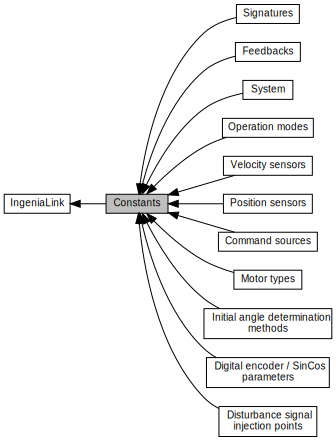
\includegraphics[width=350pt]{group__IL__CONST}
\end{center}
\end{figure}
\subsection*{Modules}
\begin{DoxyCompactItemize}
\item 
\hyperlink{group__IL__CONST__SYS}{System}
\item 
\hyperlink{group__IL__CONST__SIGNATURES}{Signatures}
\item 
\hyperlink{group__IL__CONST__OP__MODE}{Operation modes}
\item 
\hyperlink{group__IL__CONST__MOTOR}{Motor types}
\item 
\hyperlink{group__IL__CONST__FB}{Feedbacks}
\item 
\hyperlink{group__IL__CONST__VEL__SENSOR}{Velocity sensors}
\item 
\hyperlink{group__IL__CONST__POS__SENSOR}{Position sensors}
\item 
\hyperlink{group__IL__CONST__IANGLE__METHOD}{Initial angle determination methods}
\item 
\hyperlink{group__IL__CONST__DENC__SINCOS__PARAM}{Digital encoder / Sin\+Cos parameters}
\item 
\hyperlink{group__IL__CONST__DSIG__INJ}{Disturbance signal injection points}
\item 
\hyperlink{group__IL__CONST__CMD__SRC}{Command sources}
\end{DoxyCompactItemize}


\subsection{Detailed Description}

\hypertarget{group__IL__CONST__SYS}{}\section{System}
\label{group__IL__CONST__SYS}\index{System@{System}}
Collaboration diagram for System\+:\nopagebreak
\begin{figure}[H]
\begin{center}
\leavevmode
\includegraphics[width=228pt]{group__IL__CONST__SYS}
\end{center}
\end{figure}
\subsection*{Macros}
\begin{DoxyCompactItemize}
\item 
\#define \hyperlink{group__IL__CONST__SYS_gaefbce026149e3fd1ca4912e8b831e1c0}{I\+L\+K\+\_\+\+S\+Y\+S\+\_\+\+P\+W\+M\+\_\+\+M\+AX}~32767
\begin{DoxyCompactList}\small\item\em P\+WM maximum value (maximum of signed 16-\/bit). \end{DoxyCompactList}\item 
\#define \hyperlink{group__IL__CONST__SYS_gaebdf8cd11949f44b6f98507754e2eda5}{I\+L\+K\+\_\+\+S\+Y\+S\+\_\+\+C\+L\+O\+O\+P\+\_\+\+F\+R\+E\+Q\+\_\+\+T\+O\+R\+Q\+UE}~10000
\begin{DoxyCompactList}\small\item\em Current/\+Torque loop frequency (Hz). \end{DoxyCompactList}\item 
\#define \hyperlink{group__IL__CONST__SYS_gab7567b15639de41f00debc89e8cf69c1}{I\+L\+K\+\_\+\+S\+Y\+S\+\_\+\+C\+L\+O\+O\+P\+\_\+\+F\+R\+E\+Q\+\_\+\+V\+EL}~1000
\begin{DoxyCompactList}\small\item\em Velocity loop frequency (Hz). \end{DoxyCompactList}\item 
\#define \hyperlink{group__IL__CONST__SYS_ga0936a074e3c6022add3b4dd936d7472e}{I\+L\+K\+\_\+\+S\+Y\+S\+\_\+\+C\+L\+O\+O\+P\+\_\+\+F\+R\+E\+Q\+\_\+\+P\+OS}~1000
\begin{DoxyCompactList}\small\item\em Position loop frequency (Hz). \end{DoxyCompactList}\item 
\#define \hyperlink{group__IL__CONST__SYS_ga7d97997e842304310662f2b151281a9f}{I\+L\+K\+\_\+\+S\+Y\+S\+\_\+\+T\+O\+R\+Q\+U\+E\+\_\+\+M\+AX}~32767
\begin{DoxyCompactList}\small\item\em Maximum rated torque (maximum of I\+N\+T16). \end{DoxyCompactList}\item 
\#define \hyperlink{group__IL__CONST__SYS_ga67fd909fd6fa467e246a1d03aaaab058}{I\+L\+K\+\_\+\+S\+Y\+S\+\_\+\+D\+S\+I\+G\+\_\+\+M\+A\+X\+\_\+\+S\+A\+M\+P\+L\+ES}~1000
\begin{DoxyCompactList}\small\item\em Disturbance signal maximum samples. \end{DoxyCompactList}\end{DoxyCompactItemize}


\subsection{Detailed Description}


\subsection{Macro Definition Documentation}
\index{System@{System}!I\+L\+K\+\_\+\+S\+Y\+S\+\_\+\+C\+L\+O\+O\+P\+\_\+\+F\+R\+E\+Q\+\_\+\+P\+OS@{I\+L\+K\+\_\+\+S\+Y\+S\+\_\+\+C\+L\+O\+O\+P\+\_\+\+F\+R\+E\+Q\+\_\+\+P\+OS}}
\index{I\+L\+K\+\_\+\+S\+Y\+S\+\_\+\+C\+L\+O\+O\+P\+\_\+\+F\+R\+E\+Q\+\_\+\+P\+OS@{I\+L\+K\+\_\+\+S\+Y\+S\+\_\+\+C\+L\+O\+O\+P\+\_\+\+F\+R\+E\+Q\+\_\+\+P\+OS}!System@{System}}
\subsubsection[{\texorpdfstring{I\+L\+K\+\_\+\+S\+Y\+S\+\_\+\+C\+L\+O\+O\+P\+\_\+\+F\+R\+E\+Q\+\_\+\+P\+OS}{ILK_SYS_CLOOP_FREQ_POS}}]{\setlength{\rightskip}{0pt plus 5cm}\#define I\+L\+K\+\_\+\+S\+Y\+S\+\_\+\+C\+L\+O\+O\+P\+\_\+\+F\+R\+E\+Q\+\_\+\+P\+OS~1000}\hypertarget{group__IL__CONST__SYS_ga0936a074e3c6022add3b4dd936d7472e}{}\label{group__IL__CONST__SYS_ga0936a074e3c6022add3b4dd936d7472e}


Position loop frequency (Hz). 

\index{System@{System}!I\+L\+K\+\_\+\+S\+Y\+S\+\_\+\+C\+L\+O\+O\+P\+\_\+\+F\+R\+E\+Q\+\_\+\+T\+O\+R\+Q\+UE@{I\+L\+K\+\_\+\+S\+Y\+S\+\_\+\+C\+L\+O\+O\+P\+\_\+\+F\+R\+E\+Q\+\_\+\+T\+O\+R\+Q\+UE}}
\index{I\+L\+K\+\_\+\+S\+Y\+S\+\_\+\+C\+L\+O\+O\+P\+\_\+\+F\+R\+E\+Q\+\_\+\+T\+O\+R\+Q\+UE@{I\+L\+K\+\_\+\+S\+Y\+S\+\_\+\+C\+L\+O\+O\+P\+\_\+\+F\+R\+E\+Q\+\_\+\+T\+O\+R\+Q\+UE}!System@{System}}
\subsubsection[{\texorpdfstring{I\+L\+K\+\_\+\+S\+Y\+S\+\_\+\+C\+L\+O\+O\+P\+\_\+\+F\+R\+E\+Q\+\_\+\+T\+O\+R\+Q\+UE}{ILK_SYS_CLOOP_FREQ_TORQUE}}]{\setlength{\rightskip}{0pt plus 5cm}\#define I\+L\+K\+\_\+\+S\+Y\+S\+\_\+\+C\+L\+O\+O\+P\+\_\+\+F\+R\+E\+Q\+\_\+\+T\+O\+R\+Q\+UE~10000}\hypertarget{group__IL__CONST__SYS_gaebdf8cd11949f44b6f98507754e2eda5}{}\label{group__IL__CONST__SYS_gaebdf8cd11949f44b6f98507754e2eda5}


Current/\+Torque loop frequency (Hz). 

\index{System@{System}!I\+L\+K\+\_\+\+S\+Y\+S\+\_\+\+C\+L\+O\+O\+P\+\_\+\+F\+R\+E\+Q\+\_\+\+V\+EL@{I\+L\+K\+\_\+\+S\+Y\+S\+\_\+\+C\+L\+O\+O\+P\+\_\+\+F\+R\+E\+Q\+\_\+\+V\+EL}}
\index{I\+L\+K\+\_\+\+S\+Y\+S\+\_\+\+C\+L\+O\+O\+P\+\_\+\+F\+R\+E\+Q\+\_\+\+V\+EL@{I\+L\+K\+\_\+\+S\+Y\+S\+\_\+\+C\+L\+O\+O\+P\+\_\+\+F\+R\+E\+Q\+\_\+\+V\+EL}!System@{System}}
\subsubsection[{\texorpdfstring{I\+L\+K\+\_\+\+S\+Y\+S\+\_\+\+C\+L\+O\+O\+P\+\_\+\+F\+R\+E\+Q\+\_\+\+V\+EL}{ILK_SYS_CLOOP_FREQ_VEL}}]{\setlength{\rightskip}{0pt plus 5cm}\#define I\+L\+K\+\_\+\+S\+Y\+S\+\_\+\+C\+L\+O\+O\+P\+\_\+\+F\+R\+E\+Q\+\_\+\+V\+EL~1000}\hypertarget{group__IL__CONST__SYS_gab7567b15639de41f00debc89e8cf69c1}{}\label{group__IL__CONST__SYS_gab7567b15639de41f00debc89e8cf69c1}


Velocity loop frequency (Hz). 

\index{System@{System}!I\+L\+K\+\_\+\+S\+Y\+S\+\_\+\+D\+S\+I\+G\+\_\+\+M\+A\+X\+\_\+\+S\+A\+M\+P\+L\+ES@{I\+L\+K\+\_\+\+S\+Y\+S\+\_\+\+D\+S\+I\+G\+\_\+\+M\+A\+X\+\_\+\+S\+A\+M\+P\+L\+ES}}
\index{I\+L\+K\+\_\+\+S\+Y\+S\+\_\+\+D\+S\+I\+G\+\_\+\+M\+A\+X\+\_\+\+S\+A\+M\+P\+L\+ES@{I\+L\+K\+\_\+\+S\+Y\+S\+\_\+\+D\+S\+I\+G\+\_\+\+M\+A\+X\+\_\+\+S\+A\+M\+P\+L\+ES}!System@{System}}
\subsubsection[{\texorpdfstring{I\+L\+K\+\_\+\+S\+Y\+S\+\_\+\+D\+S\+I\+G\+\_\+\+M\+A\+X\+\_\+\+S\+A\+M\+P\+L\+ES}{ILK_SYS_DSIG_MAX_SAMPLES}}]{\setlength{\rightskip}{0pt plus 5cm}\#define I\+L\+K\+\_\+\+S\+Y\+S\+\_\+\+D\+S\+I\+G\+\_\+\+M\+A\+X\+\_\+\+S\+A\+M\+P\+L\+ES~1000}\hypertarget{group__IL__CONST__SYS_ga67fd909fd6fa467e246a1d03aaaab058}{}\label{group__IL__CONST__SYS_ga67fd909fd6fa467e246a1d03aaaab058}


Disturbance signal maximum samples. 

\index{System@{System}!I\+L\+K\+\_\+\+S\+Y\+S\+\_\+\+P\+W\+M\+\_\+\+M\+AX@{I\+L\+K\+\_\+\+S\+Y\+S\+\_\+\+P\+W\+M\+\_\+\+M\+AX}}
\index{I\+L\+K\+\_\+\+S\+Y\+S\+\_\+\+P\+W\+M\+\_\+\+M\+AX@{I\+L\+K\+\_\+\+S\+Y\+S\+\_\+\+P\+W\+M\+\_\+\+M\+AX}!System@{System}}
\subsubsection[{\texorpdfstring{I\+L\+K\+\_\+\+S\+Y\+S\+\_\+\+P\+W\+M\+\_\+\+M\+AX}{ILK_SYS_PWM_MAX}}]{\setlength{\rightskip}{0pt plus 5cm}\#define I\+L\+K\+\_\+\+S\+Y\+S\+\_\+\+P\+W\+M\+\_\+\+M\+AX~32767}\hypertarget{group__IL__CONST__SYS_gaefbce026149e3fd1ca4912e8b831e1c0}{}\label{group__IL__CONST__SYS_gaefbce026149e3fd1ca4912e8b831e1c0}


P\+WM maximum value (maximum of signed 16-\/bit). 

\index{System@{System}!I\+L\+K\+\_\+\+S\+Y\+S\+\_\+\+T\+O\+R\+Q\+U\+E\+\_\+\+M\+AX@{I\+L\+K\+\_\+\+S\+Y\+S\+\_\+\+T\+O\+R\+Q\+U\+E\+\_\+\+M\+AX}}
\index{I\+L\+K\+\_\+\+S\+Y\+S\+\_\+\+T\+O\+R\+Q\+U\+E\+\_\+\+M\+AX@{I\+L\+K\+\_\+\+S\+Y\+S\+\_\+\+T\+O\+R\+Q\+U\+E\+\_\+\+M\+AX}!System@{System}}
\subsubsection[{\texorpdfstring{I\+L\+K\+\_\+\+S\+Y\+S\+\_\+\+T\+O\+R\+Q\+U\+E\+\_\+\+M\+AX}{ILK_SYS_TORQUE_MAX}}]{\setlength{\rightskip}{0pt plus 5cm}\#define I\+L\+K\+\_\+\+S\+Y\+S\+\_\+\+T\+O\+R\+Q\+U\+E\+\_\+\+M\+AX~32767}\hypertarget{group__IL__CONST__SYS_ga7d97997e842304310662f2b151281a9f}{}\label{group__IL__CONST__SYS_ga7d97997e842304310662f2b151281a9f}


Maximum rated torque (maximum of I\+N\+T16). 


\hypertarget{group__IL__CONST__SIGNATURES}{}\section{Signatures}
\label{group__IL__CONST__SIGNATURES}\index{Signatures@{Signatures}}
Collaboration diagram for Signatures\+:\nopagebreak
\begin{figure}[H]
\begin{center}
\leavevmode
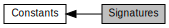
\includegraphics[width=241pt]{group__IL__CONST__SIGNATURES}
\end{center}
\end{figure}
\subsection*{Macros}
\begin{DoxyCompactItemize}
\item 
\#define \hyperlink{group__IL__CONST__SIGNATURES_ga4c86aee7016ece956e15b5d1523fbc07}{I\+L\+K\+\_\+\+S\+I\+G\+N\+A\+T\+U\+R\+E\+\_\+\+S\+T\+O\+RE}~0x65766173
\begin{DoxyCompactList}\small\item\em Store signature. \end{DoxyCompactList}\item 
\#define \hyperlink{group__IL__CONST__SIGNATURES_gafec6f03943f9194696a21de117dedbfc}{I\+L\+K\+\_\+\+S\+I\+G\+N\+A\+T\+U\+R\+E\+\_\+\+R\+E\+S\+ET}~0x64747372
\begin{DoxyCompactList}\small\item\em Reset signature. \end{DoxyCompactList}\end{DoxyCompactItemize}


\subsection{Detailed Description}


\subsection{Macro Definition Documentation}
\index{Signatures@{Signatures}!I\+L\+K\+\_\+\+S\+I\+G\+N\+A\+T\+U\+R\+E\+\_\+\+R\+E\+S\+ET@{I\+L\+K\+\_\+\+S\+I\+G\+N\+A\+T\+U\+R\+E\+\_\+\+R\+E\+S\+ET}}
\index{I\+L\+K\+\_\+\+S\+I\+G\+N\+A\+T\+U\+R\+E\+\_\+\+R\+E\+S\+ET@{I\+L\+K\+\_\+\+S\+I\+G\+N\+A\+T\+U\+R\+E\+\_\+\+R\+E\+S\+ET}!Signatures@{Signatures}}
\subsubsection[{\texorpdfstring{I\+L\+K\+\_\+\+S\+I\+G\+N\+A\+T\+U\+R\+E\+\_\+\+R\+E\+S\+ET}{ILK_SIGNATURE_RESET}}]{\setlength{\rightskip}{0pt plus 5cm}\#define I\+L\+K\+\_\+\+S\+I\+G\+N\+A\+T\+U\+R\+E\+\_\+\+R\+E\+S\+ET~0x64747372}\hypertarget{group__IL__CONST__SIGNATURES_gafec6f03943f9194696a21de117dedbfc}{}\label{group__IL__CONST__SIGNATURES_gafec6f03943f9194696a21de117dedbfc}


Reset signature. 

\index{Signatures@{Signatures}!I\+L\+K\+\_\+\+S\+I\+G\+N\+A\+T\+U\+R\+E\+\_\+\+S\+T\+O\+RE@{I\+L\+K\+\_\+\+S\+I\+G\+N\+A\+T\+U\+R\+E\+\_\+\+S\+T\+O\+RE}}
\index{I\+L\+K\+\_\+\+S\+I\+G\+N\+A\+T\+U\+R\+E\+\_\+\+S\+T\+O\+RE@{I\+L\+K\+\_\+\+S\+I\+G\+N\+A\+T\+U\+R\+E\+\_\+\+S\+T\+O\+RE}!Signatures@{Signatures}}
\subsubsection[{\texorpdfstring{I\+L\+K\+\_\+\+S\+I\+G\+N\+A\+T\+U\+R\+E\+\_\+\+S\+T\+O\+RE}{ILK_SIGNATURE_STORE}}]{\setlength{\rightskip}{0pt plus 5cm}\#define I\+L\+K\+\_\+\+S\+I\+G\+N\+A\+T\+U\+R\+E\+\_\+\+S\+T\+O\+RE~0x65766173}\hypertarget{group__IL__CONST__SIGNATURES_ga4c86aee7016ece956e15b5d1523fbc07}{}\label{group__IL__CONST__SIGNATURES_ga4c86aee7016ece956e15b5d1523fbc07}


Store signature. 


\hypertarget{group__IL__CONST__OP__MODE}{}\section{Operation modes}
\label{group__IL__CONST__OP__MODE}\index{Operation modes@{Operation modes}}
Collaboration diagram for Operation modes\+:\nopagebreak
\begin{figure}[H]
\begin{center}
\leavevmode
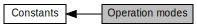
\includegraphics[width=269pt]{group__IL__CONST__OP__MODE}
\end{center}
\end{figure}
\subsection*{Macros}
\begin{DoxyCompactItemize}
\item 
\#define \hyperlink{group__IL__CONST__OP__MODE_ga1f22e168e8a3092acf6982d6374ef829}{I\+L\+K\+\_\+\+O\+P\+\_\+\+M\+O\+D\+E\+\_\+\+O\+LV}~-\/2
\begin{DoxyCompactList}\small\item\em Open loop (vector mode). \end{DoxyCompactList}\item 
\#define \hyperlink{group__IL__CONST__OP__MODE_ga0a7de45bb24cb05b8bae5a4399baef6e}{I\+L\+K\+\_\+\+O\+P\+\_\+\+M\+O\+D\+E\+\_\+\+O\+LS}~-\/1
\begin{DoxyCompactList}\small\item\em Open loop (scalar mode). \end{DoxyCompactList}\item 
\#define \hyperlink{group__IL__CONST__OP__MODE_ga52b02647597ea4e09718a62b2ee8d994}{I\+L\+K\+\_\+\+O\+P\+\_\+\+M\+O\+D\+E\+\_\+\+PP}~1
\begin{DoxyCompactList}\small\item\em Profile position. \end{DoxyCompactList}\item 
\#define \hyperlink{group__IL__CONST__OP__MODE_ga2e2b186a23f0b7d57a0f9faa590cea05}{I\+L\+K\+\_\+\+O\+P\+\_\+\+M\+O\+D\+E\+\_\+\+V\+EL}~2
\begin{DoxyCompactList}\small\item\em Velocity. \end{DoxyCompactList}\item 
\#define \hyperlink{group__IL__CONST__OP__MODE_ga835525c916eb87bd07495702423f5571}{I\+L\+K\+\_\+\+O\+P\+\_\+\+M\+O\+D\+E\+\_\+\+PV}~3
\begin{DoxyCompactList}\small\item\em Profile velocity. \end{DoxyCompactList}\item 
\#define \hyperlink{group__IL__CONST__OP__MODE_ga620365ff1869f00172b03ed1f8ea3b2f}{I\+L\+K\+\_\+\+O\+P\+\_\+\+M\+O\+D\+E\+\_\+\+PT}~4
\begin{DoxyCompactList}\small\item\em Profile torque. \end{DoxyCompactList}\item 
\#define \hyperlink{group__IL__CONST__OP__MODE_ga9f1663d81dc7e4cb79afa5cdfceded54}{I\+L\+K\+\_\+\+O\+P\+\_\+\+M\+O\+D\+E\+\_\+\+H\+O\+M\+I\+NG}~6
\begin{DoxyCompactList}\small\item\em Homing. \end{DoxyCompactList}\item 
\#define \hyperlink{group__IL__CONST__OP__MODE_ga35cf56e35484129095342ad889db552c}{I\+L\+K\+\_\+\+O\+P\+\_\+\+M\+O\+D\+E\+\_\+\+IP}~7
\begin{DoxyCompactList}\small\item\em Interpolated position mode. \end{DoxyCompactList}\item 
\#define \hyperlink{group__IL__CONST__OP__MODE_ga95c806de859172e9f09af0d620f15ec5}{I\+L\+K\+\_\+\+O\+P\+\_\+\+M\+O\+D\+E\+\_\+\+C\+SP}~8
\begin{DoxyCompactList}\small\item\em Cyclic sync position mode. \end{DoxyCompactList}\item 
\#define \hyperlink{group__IL__CONST__OP__MODE_gaaf121cd4e10a148b001f0a4d7cafae96}{I\+L\+K\+\_\+\+O\+P\+\_\+\+M\+O\+D\+E\+\_\+\+C\+SV}~9
\begin{DoxyCompactList}\small\item\em Cyclic sync velocity mode. \end{DoxyCompactList}\item 
\#define \hyperlink{group__IL__CONST__OP__MODE_ga336b0e7a48565b41d3b67cc4527b6298}{I\+L\+K\+\_\+\+O\+P\+\_\+\+M\+O\+D\+E\+\_\+\+C\+ST}~10
\begin{DoxyCompactList}\small\item\em Cyclic sync torque mode. \end{DoxyCompactList}\end{DoxyCompactItemize}


\subsection{Detailed Description}


\subsection{Macro Definition Documentation}
\index{Operation modes@{Operation modes}!I\+L\+K\+\_\+\+O\+P\+\_\+\+M\+O\+D\+E\+\_\+\+C\+SP@{I\+L\+K\+\_\+\+O\+P\+\_\+\+M\+O\+D\+E\+\_\+\+C\+SP}}
\index{I\+L\+K\+\_\+\+O\+P\+\_\+\+M\+O\+D\+E\+\_\+\+C\+SP@{I\+L\+K\+\_\+\+O\+P\+\_\+\+M\+O\+D\+E\+\_\+\+C\+SP}!Operation modes@{Operation modes}}
\subsubsection[{\texorpdfstring{I\+L\+K\+\_\+\+O\+P\+\_\+\+M\+O\+D\+E\+\_\+\+C\+SP}{ILK_OP_MODE_CSP}}]{\setlength{\rightskip}{0pt plus 5cm}\#define I\+L\+K\+\_\+\+O\+P\+\_\+\+M\+O\+D\+E\+\_\+\+C\+SP~8}\hypertarget{group__IL__CONST__OP__MODE_ga95c806de859172e9f09af0d620f15ec5}{}\label{group__IL__CONST__OP__MODE_ga95c806de859172e9f09af0d620f15ec5}


Cyclic sync position mode. 

\index{Operation modes@{Operation modes}!I\+L\+K\+\_\+\+O\+P\+\_\+\+M\+O\+D\+E\+\_\+\+C\+ST@{I\+L\+K\+\_\+\+O\+P\+\_\+\+M\+O\+D\+E\+\_\+\+C\+ST}}
\index{I\+L\+K\+\_\+\+O\+P\+\_\+\+M\+O\+D\+E\+\_\+\+C\+ST@{I\+L\+K\+\_\+\+O\+P\+\_\+\+M\+O\+D\+E\+\_\+\+C\+ST}!Operation modes@{Operation modes}}
\subsubsection[{\texorpdfstring{I\+L\+K\+\_\+\+O\+P\+\_\+\+M\+O\+D\+E\+\_\+\+C\+ST}{ILK_OP_MODE_CST}}]{\setlength{\rightskip}{0pt plus 5cm}\#define I\+L\+K\+\_\+\+O\+P\+\_\+\+M\+O\+D\+E\+\_\+\+C\+ST~10}\hypertarget{group__IL__CONST__OP__MODE_ga336b0e7a48565b41d3b67cc4527b6298}{}\label{group__IL__CONST__OP__MODE_ga336b0e7a48565b41d3b67cc4527b6298}


Cyclic sync torque mode. 

\index{Operation modes@{Operation modes}!I\+L\+K\+\_\+\+O\+P\+\_\+\+M\+O\+D\+E\+\_\+\+C\+SV@{I\+L\+K\+\_\+\+O\+P\+\_\+\+M\+O\+D\+E\+\_\+\+C\+SV}}
\index{I\+L\+K\+\_\+\+O\+P\+\_\+\+M\+O\+D\+E\+\_\+\+C\+SV@{I\+L\+K\+\_\+\+O\+P\+\_\+\+M\+O\+D\+E\+\_\+\+C\+SV}!Operation modes@{Operation modes}}
\subsubsection[{\texorpdfstring{I\+L\+K\+\_\+\+O\+P\+\_\+\+M\+O\+D\+E\+\_\+\+C\+SV}{ILK_OP_MODE_CSV}}]{\setlength{\rightskip}{0pt plus 5cm}\#define I\+L\+K\+\_\+\+O\+P\+\_\+\+M\+O\+D\+E\+\_\+\+C\+SV~9}\hypertarget{group__IL__CONST__OP__MODE_gaaf121cd4e10a148b001f0a4d7cafae96}{}\label{group__IL__CONST__OP__MODE_gaaf121cd4e10a148b001f0a4d7cafae96}


Cyclic sync velocity mode. 

\index{Operation modes@{Operation modes}!I\+L\+K\+\_\+\+O\+P\+\_\+\+M\+O\+D\+E\+\_\+\+H\+O\+M\+I\+NG@{I\+L\+K\+\_\+\+O\+P\+\_\+\+M\+O\+D\+E\+\_\+\+H\+O\+M\+I\+NG}}
\index{I\+L\+K\+\_\+\+O\+P\+\_\+\+M\+O\+D\+E\+\_\+\+H\+O\+M\+I\+NG@{I\+L\+K\+\_\+\+O\+P\+\_\+\+M\+O\+D\+E\+\_\+\+H\+O\+M\+I\+NG}!Operation modes@{Operation modes}}
\subsubsection[{\texorpdfstring{I\+L\+K\+\_\+\+O\+P\+\_\+\+M\+O\+D\+E\+\_\+\+H\+O\+M\+I\+NG}{ILK_OP_MODE_HOMING}}]{\setlength{\rightskip}{0pt plus 5cm}\#define I\+L\+K\+\_\+\+O\+P\+\_\+\+M\+O\+D\+E\+\_\+\+H\+O\+M\+I\+NG~6}\hypertarget{group__IL__CONST__OP__MODE_ga9f1663d81dc7e4cb79afa5cdfceded54}{}\label{group__IL__CONST__OP__MODE_ga9f1663d81dc7e4cb79afa5cdfceded54}


Homing. 

\index{Operation modes@{Operation modes}!I\+L\+K\+\_\+\+O\+P\+\_\+\+M\+O\+D\+E\+\_\+\+IP@{I\+L\+K\+\_\+\+O\+P\+\_\+\+M\+O\+D\+E\+\_\+\+IP}}
\index{I\+L\+K\+\_\+\+O\+P\+\_\+\+M\+O\+D\+E\+\_\+\+IP@{I\+L\+K\+\_\+\+O\+P\+\_\+\+M\+O\+D\+E\+\_\+\+IP}!Operation modes@{Operation modes}}
\subsubsection[{\texorpdfstring{I\+L\+K\+\_\+\+O\+P\+\_\+\+M\+O\+D\+E\+\_\+\+IP}{ILK_OP_MODE_IP}}]{\setlength{\rightskip}{0pt plus 5cm}\#define I\+L\+K\+\_\+\+O\+P\+\_\+\+M\+O\+D\+E\+\_\+\+IP~7}\hypertarget{group__IL__CONST__OP__MODE_ga35cf56e35484129095342ad889db552c}{}\label{group__IL__CONST__OP__MODE_ga35cf56e35484129095342ad889db552c}


Interpolated position mode. 

\index{Operation modes@{Operation modes}!I\+L\+K\+\_\+\+O\+P\+\_\+\+M\+O\+D\+E\+\_\+\+O\+LS@{I\+L\+K\+\_\+\+O\+P\+\_\+\+M\+O\+D\+E\+\_\+\+O\+LS}}
\index{I\+L\+K\+\_\+\+O\+P\+\_\+\+M\+O\+D\+E\+\_\+\+O\+LS@{I\+L\+K\+\_\+\+O\+P\+\_\+\+M\+O\+D\+E\+\_\+\+O\+LS}!Operation modes@{Operation modes}}
\subsubsection[{\texorpdfstring{I\+L\+K\+\_\+\+O\+P\+\_\+\+M\+O\+D\+E\+\_\+\+O\+LS}{ILK_OP_MODE_OLS}}]{\setlength{\rightskip}{0pt plus 5cm}\#define I\+L\+K\+\_\+\+O\+P\+\_\+\+M\+O\+D\+E\+\_\+\+O\+LS~-\/1}\hypertarget{group__IL__CONST__OP__MODE_ga0a7de45bb24cb05b8bae5a4399baef6e}{}\label{group__IL__CONST__OP__MODE_ga0a7de45bb24cb05b8bae5a4399baef6e}


Open loop (scalar mode). 

\index{Operation modes@{Operation modes}!I\+L\+K\+\_\+\+O\+P\+\_\+\+M\+O\+D\+E\+\_\+\+O\+LV@{I\+L\+K\+\_\+\+O\+P\+\_\+\+M\+O\+D\+E\+\_\+\+O\+LV}}
\index{I\+L\+K\+\_\+\+O\+P\+\_\+\+M\+O\+D\+E\+\_\+\+O\+LV@{I\+L\+K\+\_\+\+O\+P\+\_\+\+M\+O\+D\+E\+\_\+\+O\+LV}!Operation modes@{Operation modes}}
\subsubsection[{\texorpdfstring{I\+L\+K\+\_\+\+O\+P\+\_\+\+M\+O\+D\+E\+\_\+\+O\+LV}{ILK_OP_MODE_OLV}}]{\setlength{\rightskip}{0pt plus 5cm}\#define I\+L\+K\+\_\+\+O\+P\+\_\+\+M\+O\+D\+E\+\_\+\+O\+LV~-\/2}\hypertarget{group__IL__CONST__OP__MODE_ga1f22e168e8a3092acf6982d6374ef829}{}\label{group__IL__CONST__OP__MODE_ga1f22e168e8a3092acf6982d6374ef829}


Open loop (vector mode). 

\index{Operation modes@{Operation modes}!I\+L\+K\+\_\+\+O\+P\+\_\+\+M\+O\+D\+E\+\_\+\+PP@{I\+L\+K\+\_\+\+O\+P\+\_\+\+M\+O\+D\+E\+\_\+\+PP}}
\index{I\+L\+K\+\_\+\+O\+P\+\_\+\+M\+O\+D\+E\+\_\+\+PP@{I\+L\+K\+\_\+\+O\+P\+\_\+\+M\+O\+D\+E\+\_\+\+PP}!Operation modes@{Operation modes}}
\subsubsection[{\texorpdfstring{I\+L\+K\+\_\+\+O\+P\+\_\+\+M\+O\+D\+E\+\_\+\+PP}{ILK_OP_MODE_PP}}]{\setlength{\rightskip}{0pt plus 5cm}\#define I\+L\+K\+\_\+\+O\+P\+\_\+\+M\+O\+D\+E\+\_\+\+PP~1}\hypertarget{group__IL__CONST__OP__MODE_ga52b02647597ea4e09718a62b2ee8d994}{}\label{group__IL__CONST__OP__MODE_ga52b02647597ea4e09718a62b2ee8d994}


Profile position. 

\index{Operation modes@{Operation modes}!I\+L\+K\+\_\+\+O\+P\+\_\+\+M\+O\+D\+E\+\_\+\+PT@{I\+L\+K\+\_\+\+O\+P\+\_\+\+M\+O\+D\+E\+\_\+\+PT}}
\index{I\+L\+K\+\_\+\+O\+P\+\_\+\+M\+O\+D\+E\+\_\+\+PT@{I\+L\+K\+\_\+\+O\+P\+\_\+\+M\+O\+D\+E\+\_\+\+PT}!Operation modes@{Operation modes}}
\subsubsection[{\texorpdfstring{I\+L\+K\+\_\+\+O\+P\+\_\+\+M\+O\+D\+E\+\_\+\+PT}{ILK_OP_MODE_PT}}]{\setlength{\rightskip}{0pt plus 5cm}\#define I\+L\+K\+\_\+\+O\+P\+\_\+\+M\+O\+D\+E\+\_\+\+PT~4}\hypertarget{group__IL__CONST__OP__MODE_ga620365ff1869f00172b03ed1f8ea3b2f}{}\label{group__IL__CONST__OP__MODE_ga620365ff1869f00172b03ed1f8ea3b2f}


Profile torque. 

\index{Operation modes@{Operation modes}!I\+L\+K\+\_\+\+O\+P\+\_\+\+M\+O\+D\+E\+\_\+\+PV@{I\+L\+K\+\_\+\+O\+P\+\_\+\+M\+O\+D\+E\+\_\+\+PV}}
\index{I\+L\+K\+\_\+\+O\+P\+\_\+\+M\+O\+D\+E\+\_\+\+PV@{I\+L\+K\+\_\+\+O\+P\+\_\+\+M\+O\+D\+E\+\_\+\+PV}!Operation modes@{Operation modes}}
\subsubsection[{\texorpdfstring{I\+L\+K\+\_\+\+O\+P\+\_\+\+M\+O\+D\+E\+\_\+\+PV}{ILK_OP_MODE_PV}}]{\setlength{\rightskip}{0pt plus 5cm}\#define I\+L\+K\+\_\+\+O\+P\+\_\+\+M\+O\+D\+E\+\_\+\+PV~3}\hypertarget{group__IL__CONST__OP__MODE_ga835525c916eb87bd07495702423f5571}{}\label{group__IL__CONST__OP__MODE_ga835525c916eb87bd07495702423f5571}


Profile velocity. 

\index{Operation modes@{Operation modes}!I\+L\+K\+\_\+\+O\+P\+\_\+\+M\+O\+D\+E\+\_\+\+V\+EL@{I\+L\+K\+\_\+\+O\+P\+\_\+\+M\+O\+D\+E\+\_\+\+V\+EL}}
\index{I\+L\+K\+\_\+\+O\+P\+\_\+\+M\+O\+D\+E\+\_\+\+V\+EL@{I\+L\+K\+\_\+\+O\+P\+\_\+\+M\+O\+D\+E\+\_\+\+V\+EL}!Operation modes@{Operation modes}}
\subsubsection[{\texorpdfstring{I\+L\+K\+\_\+\+O\+P\+\_\+\+M\+O\+D\+E\+\_\+\+V\+EL}{ILK_OP_MODE_VEL}}]{\setlength{\rightskip}{0pt plus 5cm}\#define I\+L\+K\+\_\+\+O\+P\+\_\+\+M\+O\+D\+E\+\_\+\+V\+EL~2}\hypertarget{group__IL__CONST__OP__MODE_ga2e2b186a23f0b7d57a0f9faa590cea05}{}\label{group__IL__CONST__OP__MODE_ga2e2b186a23f0b7d57a0f9faa590cea05}


Velocity. 


\hypertarget{group__IL__CONST__MOTOR}{}\section{Motor types}
\label{group__IL__CONST__MOTOR}\index{Motor types@{Motor types}}
Collaboration diagram for Motor types\+:\nopagebreak
\begin{figure}[H]
\begin{center}
\leavevmode
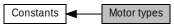
\includegraphics[width=246pt]{group__IL__CONST__MOTOR}
\end{center}
\end{figure}
\subsection*{Macros}
\begin{DoxyCompactItemize}
\item 
\#define \hyperlink{group__IL__CONST__MOTOR_ga5bdb2f869123533b63941efbb1a7aea3}{I\+L\+K\+\_\+\+M\+O\+T\+O\+R\+\_\+\+S\+Q\+U\+I\+R\+R\+EL}~0x0007
\begin{DoxyCompactList}\small\item\em Squirrel cage induction. \end{DoxyCompactList}\item 
\#define \hyperlink{group__IL__CONST__MOTOR_ga13f49aebf7a4d08b01a9c7aa00164ead}{I\+L\+K\+\_\+\+M\+O\+T\+O\+R\+\_\+\+S\+T\+E\+P\+P\+ER}~0x0009
\begin{DoxyCompactList}\small\item\em Stepper with microstepping capability. \end{DoxyCompactList}\item 
\#define \hyperlink{group__IL__CONST__MOTOR_ga9e363ce9fcb333f1a0ca43cf3e018de9}{I\+L\+K\+\_\+\+M\+O\+T\+O\+R\+\_\+\+R\+O\+T\+\_\+\+B\+L\+AC}~0x000A
\begin{DoxyCompactList}\small\item\em Rotary brushless AC. \end{DoxyCompactList}\item 
\#define \hyperlink{group__IL__CONST__MOTOR_ga1b190d9b607368d639ccfd6b61d27616}{I\+L\+K\+\_\+\+M\+O\+T\+O\+R\+\_\+\+R\+O\+T\+\_\+\+B\+L\+DC}~0x000B
\begin{DoxyCompactList}\small\item\em Rotary brushless DC. \end{DoxyCompactList}\item 
\#define \hyperlink{group__IL__CONST__MOTOR_ga1f7f2854dad7608e3f814d9409866ccc}{I\+L\+K\+\_\+\+M\+O\+T\+O\+R\+\_\+\+R\+O\+T\+\_\+\+DC}~0x000D
\begin{DoxyCompactList}\small\item\em Rotary DC. \end{DoxyCompactList}\item 
\#define \hyperlink{group__IL__CONST__MOTOR_ga7ce94e9b64195dad671ec5bc25938f78}{I\+L\+K\+\_\+\+M\+O\+T\+O\+R\+\_\+\+R\+O\+T\+\_\+\+VC}~0x8000
\begin{DoxyCompactList}\small\item\em Rotary voice coil. \end{DoxyCompactList}\item 
\#define \hyperlink{group__IL__CONST__MOTOR_ga4e9537c5560f52a0c69d5cfe9e06f4af}{I\+L\+K\+\_\+\+M\+O\+T\+O\+R\+\_\+\+L\+I\+N\+\_\+\+B\+L\+AC}~0x8001
\begin{DoxyCompactList}\small\item\em Linear brushless AC. \end{DoxyCompactList}\item 
\#define \hyperlink{group__IL__CONST__MOTOR_gafb0b611a2644cf1673896daf236b69b7}{I\+L\+K\+\_\+\+M\+O\+T\+O\+R\+\_\+\+L\+I\+N\+\_\+\+B\+L\+DC}~0x8002
\begin{DoxyCompactList}\small\item\em Linear brushless DC. \end{DoxyCompactList}\item 
\#define \hyperlink{group__IL__CONST__MOTOR_gad90b5df2f58dc0a6ff0452abdc0f0e22}{I\+L\+K\+\_\+\+M\+O\+T\+O\+R\+\_\+\+L\+I\+N\+\_\+\+VC}~0x8003
\begin{DoxyCompactList}\small\item\em Linear voice coil. \end{DoxyCompactList}\item 
\#define \hyperlink{group__IL__CONST__MOTOR_ga023e91fb0fb03bd5273e90c1399336f9}{I\+L\+K\+\_\+\+M\+O\+T\+O\+R\+\_\+\+L\+I\+N\+\_\+\+DC}~0x8004\hypertarget{group__IL__CONST__MOTOR_ga023e91fb0fb03bd5273e90c1399336f9}{}\label{group__IL__CONST__MOTOR_ga023e91fb0fb03bd5273e90c1399336f9}

\begin{DoxyCompactList}\small\item\em Linear DC. \end{DoxyCompactList}\end{DoxyCompactItemize}


\subsection{Detailed Description}


\subsection{Macro Definition Documentation}
\index{Motor types@{Motor types}!I\+L\+K\+\_\+\+M\+O\+T\+O\+R\+\_\+\+L\+I\+N\+\_\+\+B\+L\+AC@{I\+L\+K\+\_\+\+M\+O\+T\+O\+R\+\_\+\+L\+I\+N\+\_\+\+B\+L\+AC}}
\index{I\+L\+K\+\_\+\+M\+O\+T\+O\+R\+\_\+\+L\+I\+N\+\_\+\+B\+L\+AC@{I\+L\+K\+\_\+\+M\+O\+T\+O\+R\+\_\+\+L\+I\+N\+\_\+\+B\+L\+AC}!Motor types@{Motor types}}
\subsubsection[{\texorpdfstring{I\+L\+K\+\_\+\+M\+O\+T\+O\+R\+\_\+\+L\+I\+N\+\_\+\+B\+L\+AC}{ILK_MOTOR_LIN_BLAC}}]{\setlength{\rightskip}{0pt plus 5cm}\#define I\+L\+K\+\_\+\+M\+O\+T\+O\+R\+\_\+\+L\+I\+N\+\_\+\+B\+L\+AC~0x8001}\hypertarget{group__IL__CONST__MOTOR_ga4e9537c5560f52a0c69d5cfe9e06f4af}{}\label{group__IL__CONST__MOTOR_ga4e9537c5560f52a0c69d5cfe9e06f4af}


Linear brushless AC. 

\index{Motor types@{Motor types}!I\+L\+K\+\_\+\+M\+O\+T\+O\+R\+\_\+\+L\+I\+N\+\_\+\+B\+L\+DC@{I\+L\+K\+\_\+\+M\+O\+T\+O\+R\+\_\+\+L\+I\+N\+\_\+\+B\+L\+DC}}
\index{I\+L\+K\+\_\+\+M\+O\+T\+O\+R\+\_\+\+L\+I\+N\+\_\+\+B\+L\+DC@{I\+L\+K\+\_\+\+M\+O\+T\+O\+R\+\_\+\+L\+I\+N\+\_\+\+B\+L\+DC}!Motor types@{Motor types}}
\subsubsection[{\texorpdfstring{I\+L\+K\+\_\+\+M\+O\+T\+O\+R\+\_\+\+L\+I\+N\+\_\+\+B\+L\+DC}{ILK_MOTOR_LIN_BLDC}}]{\setlength{\rightskip}{0pt plus 5cm}\#define I\+L\+K\+\_\+\+M\+O\+T\+O\+R\+\_\+\+L\+I\+N\+\_\+\+B\+L\+DC~0x8002}\hypertarget{group__IL__CONST__MOTOR_gafb0b611a2644cf1673896daf236b69b7}{}\label{group__IL__CONST__MOTOR_gafb0b611a2644cf1673896daf236b69b7}


Linear brushless DC. 

\index{Motor types@{Motor types}!I\+L\+K\+\_\+\+M\+O\+T\+O\+R\+\_\+\+L\+I\+N\+\_\+\+VC@{I\+L\+K\+\_\+\+M\+O\+T\+O\+R\+\_\+\+L\+I\+N\+\_\+\+VC}}
\index{I\+L\+K\+\_\+\+M\+O\+T\+O\+R\+\_\+\+L\+I\+N\+\_\+\+VC@{I\+L\+K\+\_\+\+M\+O\+T\+O\+R\+\_\+\+L\+I\+N\+\_\+\+VC}!Motor types@{Motor types}}
\subsubsection[{\texorpdfstring{I\+L\+K\+\_\+\+M\+O\+T\+O\+R\+\_\+\+L\+I\+N\+\_\+\+VC}{ILK_MOTOR_LIN_VC}}]{\setlength{\rightskip}{0pt plus 5cm}\#define I\+L\+K\+\_\+\+M\+O\+T\+O\+R\+\_\+\+L\+I\+N\+\_\+\+VC~0x8003}\hypertarget{group__IL__CONST__MOTOR_gad90b5df2f58dc0a6ff0452abdc0f0e22}{}\label{group__IL__CONST__MOTOR_gad90b5df2f58dc0a6ff0452abdc0f0e22}


Linear voice coil. 

\index{Motor types@{Motor types}!I\+L\+K\+\_\+\+M\+O\+T\+O\+R\+\_\+\+R\+O\+T\+\_\+\+B\+L\+AC@{I\+L\+K\+\_\+\+M\+O\+T\+O\+R\+\_\+\+R\+O\+T\+\_\+\+B\+L\+AC}}
\index{I\+L\+K\+\_\+\+M\+O\+T\+O\+R\+\_\+\+R\+O\+T\+\_\+\+B\+L\+AC@{I\+L\+K\+\_\+\+M\+O\+T\+O\+R\+\_\+\+R\+O\+T\+\_\+\+B\+L\+AC}!Motor types@{Motor types}}
\subsubsection[{\texorpdfstring{I\+L\+K\+\_\+\+M\+O\+T\+O\+R\+\_\+\+R\+O\+T\+\_\+\+B\+L\+AC}{ILK_MOTOR_ROT_BLAC}}]{\setlength{\rightskip}{0pt plus 5cm}\#define I\+L\+K\+\_\+\+M\+O\+T\+O\+R\+\_\+\+R\+O\+T\+\_\+\+B\+L\+AC~0x000A}\hypertarget{group__IL__CONST__MOTOR_ga9e363ce9fcb333f1a0ca43cf3e018de9}{}\label{group__IL__CONST__MOTOR_ga9e363ce9fcb333f1a0ca43cf3e018de9}


Rotary brushless AC. 

\index{Motor types@{Motor types}!I\+L\+K\+\_\+\+M\+O\+T\+O\+R\+\_\+\+R\+O\+T\+\_\+\+B\+L\+DC@{I\+L\+K\+\_\+\+M\+O\+T\+O\+R\+\_\+\+R\+O\+T\+\_\+\+B\+L\+DC}}
\index{I\+L\+K\+\_\+\+M\+O\+T\+O\+R\+\_\+\+R\+O\+T\+\_\+\+B\+L\+DC@{I\+L\+K\+\_\+\+M\+O\+T\+O\+R\+\_\+\+R\+O\+T\+\_\+\+B\+L\+DC}!Motor types@{Motor types}}
\subsubsection[{\texorpdfstring{I\+L\+K\+\_\+\+M\+O\+T\+O\+R\+\_\+\+R\+O\+T\+\_\+\+B\+L\+DC}{ILK_MOTOR_ROT_BLDC}}]{\setlength{\rightskip}{0pt plus 5cm}\#define I\+L\+K\+\_\+\+M\+O\+T\+O\+R\+\_\+\+R\+O\+T\+\_\+\+B\+L\+DC~0x000B}\hypertarget{group__IL__CONST__MOTOR_ga1b190d9b607368d639ccfd6b61d27616}{}\label{group__IL__CONST__MOTOR_ga1b190d9b607368d639ccfd6b61d27616}


Rotary brushless DC. 

\index{Motor types@{Motor types}!I\+L\+K\+\_\+\+M\+O\+T\+O\+R\+\_\+\+R\+O\+T\+\_\+\+DC@{I\+L\+K\+\_\+\+M\+O\+T\+O\+R\+\_\+\+R\+O\+T\+\_\+\+DC}}
\index{I\+L\+K\+\_\+\+M\+O\+T\+O\+R\+\_\+\+R\+O\+T\+\_\+\+DC@{I\+L\+K\+\_\+\+M\+O\+T\+O\+R\+\_\+\+R\+O\+T\+\_\+\+DC}!Motor types@{Motor types}}
\subsubsection[{\texorpdfstring{I\+L\+K\+\_\+\+M\+O\+T\+O\+R\+\_\+\+R\+O\+T\+\_\+\+DC}{ILK_MOTOR_ROT_DC}}]{\setlength{\rightskip}{0pt plus 5cm}\#define I\+L\+K\+\_\+\+M\+O\+T\+O\+R\+\_\+\+R\+O\+T\+\_\+\+DC~0x000D}\hypertarget{group__IL__CONST__MOTOR_ga1f7f2854dad7608e3f814d9409866ccc}{}\label{group__IL__CONST__MOTOR_ga1f7f2854dad7608e3f814d9409866ccc}


Rotary DC. 

\index{Motor types@{Motor types}!I\+L\+K\+\_\+\+M\+O\+T\+O\+R\+\_\+\+R\+O\+T\+\_\+\+VC@{I\+L\+K\+\_\+\+M\+O\+T\+O\+R\+\_\+\+R\+O\+T\+\_\+\+VC}}
\index{I\+L\+K\+\_\+\+M\+O\+T\+O\+R\+\_\+\+R\+O\+T\+\_\+\+VC@{I\+L\+K\+\_\+\+M\+O\+T\+O\+R\+\_\+\+R\+O\+T\+\_\+\+VC}!Motor types@{Motor types}}
\subsubsection[{\texorpdfstring{I\+L\+K\+\_\+\+M\+O\+T\+O\+R\+\_\+\+R\+O\+T\+\_\+\+VC}{ILK_MOTOR_ROT_VC}}]{\setlength{\rightskip}{0pt plus 5cm}\#define I\+L\+K\+\_\+\+M\+O\+T\+O\+R\+\_\+\+R\+O\+T\+\_\+\+VC~0x8000}\hypertarget{group__IL__CONST__MOTOR_ga7ce94e9b64195dad671ec5bc25938f78}{}\label{group__IL__CONST__MOTOR_ga7ce94e9b64195dad671ec5bc25938f78}


Rotary voice coil. 

\index{Motor types@{Motor types}!I\+L\+K\+\_\+\+M\+O\+T\+O\+R\+\_\+\+S\+Q\+U\+I\+R\+R\+EL@{I\+L\+K\+\_\+\+M\+O\+T\+O\+R\+\_\+\+S\+Q\+U\+I\+R\+R\+EL}}
\index{I\+L\+K\+\_\+\+M\+O\+T\+O\+R\+\_\+\+S\+Q\+U\+I\+R\+R\+EL@{I\+L\+K\+\_\+\+M\+O\+T\+O\+R\+\_\+\+S\+Q\+U\+I\+R\+R\+EL}!Motor types@{Motor types}}
\subsubsection[{\texorpdfstring{I\+L\+K\+\_\+\+M\+O\+T\+O\+R\+\_\+\+S\+Q\+U\+I\+R\+R\+EL}{ILK_MOTOR_SQUIRREL}}]{\setlength{\rightskip}{0pt plus 5cm}\#define I\+L\+K\+\_\+\+M\+O\+T\+O\+R\+\_\+\+S\+Q\+U\+I\+R\+R\+EL~0x0007}\hypertarget{group__IL__CONST__MOTOR_ga5bdb2f869123533b63941efbb1a7aea3}{}\label{group__IL__CONST__MOTOR_ga5bdb2f869123533b63941efbb1a7aea3}


Squirrel cage induction. 

\index{Motor types@{Motor types}!I\+L\+K\+\_\+\+M\+O\+T\+O\+R\+\_\+\+S\+T\+E\+P\+P\+ER@{I\+L\+K\+\_\+\+M\+O\+T\+O\+R\+\_\+\+S\+T\+E\+P\+P\+ER}}
\index{I\+L\+K\+\_\+\+M\+O\+T\+O\+R\+\_\+\+S\+T\+E\+P\+P\+ER@{I\+L\+K\+\_\+\+M\+O\+T\+O\+R\+\_\+\+S\+T\+E\+P\+P\+ER}!Motor types@{Motor types}}
\subsubsection[{\texorpdfstring{I\+L\+K\+\_\+\+M\+O\+T\+O\+R\+\_\+\+S\+T\+E\+P\+P\+ER}{ILK_MOTOR_STEPPER}}]{\setlength{\rightskip}{0pt plus 5cm}\#define I\+L\+K\+\_\+\+M\+O\+T\+O\+R\+\_\+\+S\+T\+E\+P\+P\+ER~0x0009}\hypertarget{group__IL__CONST__MOTOR_ga13f49aebf7a4d08b01a9c7aa00164ead}{}\label{group__IL__CONST__MOTOR_ga13f49aebf7a4d08b01a9c7aa00164ead}


Stepper with microstepping capability. 


\hypertarget{group__IL__CONST__FB}{}\section{Feedbacks}
\label{group__IL__CONST__FB}\index{Feedbacks@{Feedbacks}}
Collaboration diagram for Feedbacks\+:\nopagebreak
\begin{figure}[H]
\begin{center}
\leavevmode
\includegraphics[width=243pt]{group__IL__CONST__FB}
\end{center}
\end{figure}
\subsection*{Macros}
\begin{DoxyCompactItemize}
\item 
\#define \hyperlink{group__IL__CONST__FB_gae3ff92eb789c2fec9b7a629b20418af1}{I\+L\+K\+\_\+\+F\+B\+\_\+\+D\+I\+G\+I\+T\+A\+L\+\_\+\+E\+N\+C\+O\+D\+ER}~0x00
\begin{DoxyCompactList}\small\item\em Digital encoder. \end{DoxyCompactList}\item 
\#define \hyperlink{group__IL__CONST__FB_ga624f38df3393c8c74ca8f350f1acfb7b}{I\+L\+K\+\_\+\+F\+B\+\_\+\+D\+I\+G\+I\+T\+A\+L\+\_\+\+H\+A\+L\+LS}~0x01
\begin{DoxyCompactList}\small\item\em Digital halls. \end{DoxyCompactList}\item 
\#define \hyperlink{group__IL__CONST__FB_gada00d2cfc8c349a4976600232b399a2c}{I\+L\+K\+\_\+\+F\+B\+\_\+\+A\+N\+A\+L\+O\+G\+\_\+\+H\+A\+L\+LS}~0x02
\begin{DoxyCompactList}\small\item\em Analog halls. \end{DoxyCompactList}\item 
\#define \hyperlink{group__IL__CONST__FB_ga03d870b0c6512ec965806036c6878ebb}{I\+L\+K\+\_\+\+F\+B\+\_\+\+A\+N\+A\+L\+O\+G\+\_\+\+I\+N\+P\+UT}~0x04
\begin{DoxyCompactList}\small\item\em Analog input. \end{DoxyCompactList}\item 
\#define \hyperlink{group__IL__CONST__FB_ga9874ed60d637b9bf51850678add98685}{I\+L\+K\+\_\+\+F\+B\+\_\+\+S\+SI}~0x05
\begin{DoxyCompactList}\small\item\em S\+SI. \end{DoxyCompactList}\item 
\#define \hyperlink{group__IL__CONST__FB_ga06e050308174827bf2f5de8c1fb18340}{I\+L\+K\+\_\+\+F\+B\+\_\+\+S\+I\+N\+C\+OS}~0x06
\begin{DoxyCompactList}\small\item\em Sin\+Cos. \end{DoxyCompactList}\item 
\#define \hyperlink{group__IL__CONST__FB_ga43f62e2c2cc014a82a93c76a11ad8106}{I\+L\+K\+\_\+\+F\+B\+\_\+\+P\+WM}~0x07
\begin{DoxyCompactList}\small\item\em P\+WM. \end{DoxyCompactList}\item 
\#define \hyperlink{group__IL__CONST__FB_ga50a41df2322b1b41b9ec93ec2fbe4811}{I\+L\+K\+\_\+\+F\+B\+\_\+\+R\+E\+S\+O\+L\+V\+ER}~0x08
\begin{DoxyCompactList}\small\item\em Resolver. \end{DoxyCompactList}\item 
\#define \hyperlink{group__IL__CONST__FB_ga4caccef6137e2cce88d4c230fe9be977}{I\+L\+K\+\_\+\+F\+B\+\_\+\+N\+O\+NE}~0x09
\begin{DoxyCompactList}\small\item\em None. \end{DoxyCompactList}\item 
\#define \hyperlink{group__IL__CONST__FB_gaa3a26923923455feb238d74ec5d64a3c}{I\+L\+K\+\_\+\+F\+B\+\_\+\+S\+I\+M\+U\+L\+A\+T\+ED}~0x0B
\begin{DoxyCompactList}\small\item\em Simulated. \end{DoxyCompactList}\end{DoxyCompactItemize}


\subsection{Detailed Description}


\subsection{Macro Definition Documentation}
\index{Feedbacks@{Feedbacks}!I\+L\+K\+\_\+\+F\+B\+\_\+\+A\+N\+A\+L\+O\+G\+\_\+\+H\+A\+L\+LS@{I\+L\+K\+\_\+\+F\+B\+\_\+\+A\+N\+A\+L\+O\+G\+\_\+\+H\+A\+L\+LS}}
\index{I\+L\+K\+\_\+\+F\+B\+\_\+\+A\+N\+A\+L\+O\+G\+\_\+\+H\+A\+L\+LS@{I\+L\+K\+\_\+\+F\+B\+\_\+\+A\+N\+A\+L\+O\+G\+\_\+\+H\+A\+L\+LS}!Feedbacks@{Feedbacks}}
\subsubsection[{\texorpdfstring{I\+L\+K\+\_\+\+F\+B\+\_\+\+A\+N\+A\+L\+O\+G\+\_\+\+H\+A\+L\+LS}{ILK_FB_ANALOG_HALLS}}]{\setlength{\rightskip}{0pt plus 5cm}\#define I\+L\+K\+\_\+\+F\+B\+\_\+\+A\+N\+A\+L\+O\+G\+\_\+\+H\+A\+L\+LS~0x02}\hypertarget{group__IL__CONST__FB_gada00d2cfc8c349a4976600232b399a2c}{}\label{group__IL__CONST__FB_gada00d2cfc8c349a4976600232b399a2c}


Analog halls. 

\index{Feedbacks@{Feedbacks}!I\+L\+K\+\_\+\+F\+B\+\_\+\+A\+N\+A\+L\+O\+G\+\_\+\+I\+N\+P\+UT@{I\+L\+K\+\_\+\+F\+B\+\_\+\+A\+N\+A\+L\+O\+G\+\_\+\+I\+N\+P\+UT}}
\index{I\+L\+K\+\_\+\+F\+B\+\_\+\+A\+N\+A\+L\+O\+G\+\_\+\+I\+N\+P\+UT@{I\+L\+K\+\_\+\+F\+B\+\_\+\+A\+N\+A\+L\+O\+G\+\_\+\+I\+N\+P\+UT}!Feedbacks@{Feedbacks}}
\subsubsection[{\texorpdfstring{I\+L\+K\+\_\+\+F\+B\+\_\+\+A\+N\+A\+L\+O\+G\+\_\+\+I\+N\+P\+UT}{ILK_FB_ANALOG_INPUT}}]{\setlength{\rightskip}{0pt plus 5cm}\#define I\+L\+K\+\_\+\+F\+B\+\_\+\+A\+N\+A\+L\+O\+G\+\_\+\+I\+N\+P\+UT~0x04}\hypertarget{group__IL__CONST__FB_ga03d870b0c6512ec965806036c6878ebb}{}\label{group__IL__CONST__FB_ga03d870b0c6512ec965806036c6878ebb}


Analog input. 

\index{Feedbacks@{Feedbacks}!I\+L\+K\+\_\+\+F\+B\+\_\+\+D\+I\+G\+I\+T\+A\+L\+\_\+\+E\+N\+C\+O\+D\+ER@{I\+L\+K\+\_\+\+F\+B\+\_\+\+D\+I\+G\+I\+T\+A\+L\+\_\+\+E\+N\+C\+O\+D\+ER}}
\index{I\+L\+K\+\_\+\+F\+B\+\_\+\+D\+I\+G\+I\+T\+A\+L\+\_\+\+E\+N\+C\+O\+D\+ER@{I\+L\+K\+\_\+\+F\+B\+\_\+\+D\+I\+G\+I\+T\+A\+L\+\_\+\+E\+N\+C\+O\+D\+ER}!Feedbacks@{Feedbacks}}
\subsubsection[{\texorpdfstring{I\+L\+K\+\_\+\+F\+B\+\_\+\+D\+I\+G\+I\+T\+A\+L\+\_\+\+E\+N\+C\+O\+D\+ER}{ILK_FB_DIGITAL_ENCODER}}]{\setlength{\rightskip}{0pt plus 5cm}\#define I\+L\+K\+\_\+\+F\+B\+\_\+\+D\+I\+G\+I\+T\+A\+L\+\_\+\+E\+N\+C\+O\+D\+ER~0x00}\hypertarget{group__IL__CONST__FB_gae3ff92eb789c2fec9b7a629b20418af1}{}\label{group__IL__CONST__FB_gae3ff92eb789c2fec9b7a629b20418af1}


Digital encoder. 

\index{Feedbacks@{Feedbacks}!I\+L\+K\+\_\+\+F\+B\+\_\+\+D\+I\+G\+I\+T\+A\+L\+\_\+\+H\+A\+L\+LS@{I\+L\+K\+\_\+\+F\+B\+\_\+\+D\+I\+G\+I\+T\+A\+L\+\_\+\+H\+A\+L\+LS}}
\index{I\+L\+K\+\_\+\+F\+B\+\_\+\+D\+I\+G\+I\+T\+A\+L\+\_\+\+H\+A\+L\+LS@{I\+L\+K\+\_\+\+F\+B\+\_\+\+D\+I\+G\+I\+T\+A\+L\+\_\+\+H\+A\+L\+LS}!Feedbacks@{Feedbacks}}
\subsubsection[{\texorpdfstring{I\+L\+K\+\_\+\+F\+B\+\_\+\+D\+I\+G\+I\+T\+A\+L\+\_\+\+H\+A\+L\+LS}{ILK_FB_DIGITAL_HALLS}}]{\setlength{\rightskip}{0pt plus 5cm}\#define I\+L\+K\+\_\+\+F\+B\+\_\+\+D\+I\+G\+I\+T\+A\+L\+\_\+\+H\+A\+L\+LS~0x01}\hypertarget{group__IL__CONST__FB_ga624f38df3393c8c74ca8f350f1acfb7b}{}\label{group__IL__CONST__FB_ga624f38df3393c8c74ca8f350f1acfb7b}


Digital halls. 

\index{Feedbacks@{Feedbacks}!I\+L\+K\+\_\+\+F\+B\+\_\+\+N\+O\+NE@{I\+L\+K\+\_\+\+F\+B\+\_\+\+N\+O\+NE}}
\index{I\+L\+K\+\_\+\+F\+B\+\_\+\+N\+O\+NE@{I\+L\+K\+\_\+\+F\+B\+\_\+\+N\+O\+NE}!Feedbacks@{Feedbacks}}
\subsubsection[{\texorpdfstring{I\+L\+K\+\_\+\+F\+B\+\_\+\+N\+O\+NE}{ILK_FB_NONE}}]{\setlength{\rightskip}{0pt plus 5cm}\#define I\+L\+K\+\_\+\+F\+B\+\_\+\+N\+O\+NE~0x09}\hypertarget{group__IL__CONST__FB_ga4caccef6137e2cce88d4c230fe9be977}{}\label{group__IL__CONST__FB_ga4caccef6137e2cce88d4c230fe9be977}


None. 

\index{Feedbacks@{Feedbacks}!I\+L\+K\+\_\+\+F\+B\+\_\+\+P\+WM@{I\+L\+K\+\_\+\+F\+B\+\_\+\+P\+WM}}
\index{I\+L\+K\+\_\+\+F\+B\+\_\+\+P\+WM@{I\+L\+K\+\_\+\+F\+B\+\_\+\+P\+WM}!Feedbacks@{Feedbacks}}
\subsubsection[{\texorpdfstring{I\+L\+K\+\_\+\+F\+B\+\_\+\+P\+WM}{ILK_FB_PWM}}]{\setlength{\rightskip}{0pt plus 5cm}\#define I\+L\+K\+\_\+\+F\+B\+\_\+\+P\+WM~0x07}\hypertarget{group__IL__CONST__FB_ga43f62e2c2cc014a82a93c76a11ad8106}{}\label{group__IL__CONST__FB_ga43f62e2c2cc014a82a93c76a11ad8106}


P\+WM. 

\index{Feedbacks@{Feedbacks}!I\+L\+K\+\_\+\+F\+B\+\_\+\+R\+E\+S\+O\+L\+V\+ER@{I\+L\+K\+\_\+\+F\+B\+\_\+\+R\+E\+S\+O\+L\+V\+ER}}
\index{I\+L\+K\+\_\+\+F\+B\+\_\+\+R\+E\+S\+O\+L\+V\+ER@{I\+L\+K\+\_\+\+F\+B\+\_\+\+R\+E\+S\+O\+L\+V\+ER}!Feedbacks@{Feedbacks}}
\subsubsection[{\texorpdfstring{I\+L\+K\+\_\+\+F\+B\+\_\+\+R\+E\+S\+O\+L\+V\+ER}{ILK_FB_RESOLVER}}]{\setlength{\rightskip}{0pt plus 5cm}\#define I\+L\+K\+\_\+\+F\+B\+\_\+\+R\+E\+S\+O\+L\+V\+ER~0x08}\hypertarget{group__IL__CONST__FB_ga50a41df2322b1b41b9ec93ec2fbe4811}{}\label{group__IL__CONST__FB_ga50a41df2322b1b41b9ec93ec2fbe4811}


Resolver. 

\index{Feedbacks@{Feedbacks}!I\+L\+K\+\_\+\+F\+B\+\_\+\+S\+I\+M\+U\+L\+A\+T\+ED@{I\+L\+K\+\_\+\+F\+B\+\_\+\+S\+I\+M\+U\+L\+A\+T\+ED}}
\index{I\+L\+K\+\_\+\+F\+B\+\_\+\+S\+I\+M\+U\+L\+A\+T\+ED@{I\+L\+K\+\_\+\+F\+B\+\_\+\+S\+I\+M\+U\+L\+A\+T\+ED}!Feedbacks@{Feedbacks}}
\subsubsection[{\texorpdfstring{I\+L\+K\+\_\+\+F\+B\+\_\+\+S\+I\+M\+U\+L\+A\+T\+ED}{ILK_FB_SIMULATED}}]{\setlength{\rightskip}{0pt plus 5cm}\#define I\+L\+K\+\_\+\+F\+B\+\_\+\+S\+I\+M\+U\+L\+A\+T\+ED~0x0B}\hypertarget{group__IL__CONST__FB_gaa3a26923923455feb238d74ec5d64a3c}{}\label{group__IL__CONST__FB_gaa3a26923923455feb238d74ec5d64a3c}


Simulated. 

\index{Feedbacks@{Feedbacks}!I\+L\+K\+\_\+\+F\+B\+\_\+\+S\+I\+N\+C\+OS@{I\+L\+K\+\_\+\+F\+B\+\_\+\+S\+I\+N\+C\+OS}}
\index{I\+L\+K\+\_\+\+F\+B\+\_\+\+S\+I\+N\+C\+OS@{I\+L\+K\+\_\+\+F\+B\+\_\+\+S\+I\+N\+C\+OS}!Feedbacks@{Feedbacks}}
\subsubsection[{\texorpdfstring{I\+L\+K\+\_\+\+F\+B\+\_\+\+S\+I\+N\+C\+OS}{ILK_FB_SINCOS}}]{\setlength{\rightskip}{0pt plus 5cm}\#define I\+L\+K\+\_\+\+F\+B\+\_\+\+S\+I\+N\+C\+OS~0x06}\hypertarget{group__IL__CONST__FB_ga06e050308174827bf2f5de8c1fb18340}{}\label{group__IL__CONST__FB_ga06e050308174827bf2f5de8c1fb18340}


Sin\+Cos. 

\index{Feedbacks@{Feedbacks}!I\+L\+K\+\_\+\+F\+B\+\_\+\+S\+SI@{I\+L\+K\+\_\+\+F\+B\+\_\+\+S\+SI}}
\index{I\+L\+K\+\_\+\+F\+B\+\_\+\+S\+SI@{I\+L\+K\+\_\+\+F\+B\+\_\+\+S\+SI}!Feedbacks@{Feedbacks}}
\subsubsection[{\texorpdfstring{I\+L\+K\+\_\+\+F\+B\+\_\+\+S\+SI}{ILK_FB_SSI}}]{\setlength{\rightskip}{0pt plus 5cm}\#define I\+L\+K\+\_\+\+F\+B\+\_\+\+S\+SI~0x05}\hypertarget{group__IL__CONST__FB_ga9874ed60d637b9bf51850678add98685}{}\label{group__IL__CONST__FB_ga9874ed60d637b9bf51850678add98685}


S\+SI. 


\hypertarget{group__IL__CONST__VEL__SENSOR}{}\section{Velocity sensors}
\label{group__IL__CONST__VEL__SENSOR}\index{Velocity sensors@{Velocity sensors}}
Collaboration diagram for Velocity sensors\+:\nopagebreak
\begin{figure}[H]
\begin{center}
\leavevmode
\includegraphics[width=267pt]{group__IL__CONST__VEL__SENSOR}
\end{center}
\end{figure}
\subsection*{Macros}
\begin{DoxyCompactItemize}
\item 
\#define \hyperlink{group__IL__CONST__VEL__SENSOR_ga84b8ae078f55b0fe678b42ba33ecbffb}{I\+L\+K\+\_\+\+V\+E\+L\+\_\+\+S\+E\+N\+S\+O\+R\+\_\+\+P\+OS}~0x00
\begin{DoxyCompactList}\small\item\em Position sensor. \end{DoxyCompactList}\item 
\#define \hyperlink{group__IL__CONST__VEL__SENSOR_ga5e2000096458f2759519f81411f2f25e}{I\+L\+K\+\_\+\+V\+E\+L\+\_\+\+S\+E\+N\+S\+O\+R\+\_\+\+T\+A\+C\+H\+O\+M\+E\+T\+ER}~0x01
\begin{DoxyCompactList}\small\item\em External DC tachometer. \end{DoxyCompactList}\item 
\#define \hyperlink{group__IL__CONST__VEL__SENSOR_gadf37b8bf88afd7b938ac2edf99474553}{I\+L\+K\+\_\+\+V\+E\+L\+\_\+\+S\+E\+N\+S\+O\+R\+\_\+\+N\+O\+NE}~0x02
\begin{DoxyCompactList}\small\item\em None. \end{DoxyCompactList}\item 
\#define \hyperlink{group__IL__CONST__VEL__SENSOR_ga245f70defaf3b4a986ef63ae406db0df}{I\+L\+K\+\_\+\+V\+E\+L\+\_\+\+S\+E\+N\+S\+O\+R\+\_\+\+D\+I\+G\+I\+T\+A\+L\+\_\+\+H\+A\+L\+LS}~0x04
\begin{DoxyCompactList}\small\item\em Digital halls. \end{DoxyCompactList}\end{DoxyCompactItemize}


\subsection{Detailed Description}


\subsection{Macro Definition Documentation}
\index{Velocity sensors@{Velocity sensors}!I\+L\+K\+\_\+\+V\+E\+L\+\_\+\+S\+E\+N\+S\+O\+R\+\_\+\+D\+I\+G\+I\+T\+A\+L\+\_\+\+H\+A\+L\+LS@{I\+L\+K\+\_\+\+V\+E\+L\+\_\+\+S\+E\+N\+S\+O\+R\+\_\+\+D\+I\+G\+I\+T\+A\+L\+\_\+\+H\+A\+L\+LS}}
\index{I\+L\+K\+\_\+\+V\+E\+L\+\_\+\+S\+E\+N\+S\+O\+R\+\_\+\+D\+I\+G\+I\+T\+A\+L\+\_\+\+H\+A\+L\+LS@{I\+L\+K\+\_\+\+V\+E\+L\+\_\+\+S\+E\+N\+S\+O\+R\+\_\+\+D\+I\+G\+I\+T\+A\+L\+\_\+\+H\+A\+L\+LS}!Velocity sensors@{Velocity sensors}}
\subsubsection[{\texorpdfstring{I\+L\+K\+\_\+\+V\+E\+L\+\_\+\+S\+E\+N\+S\+O\+R\+\_\+\+D\+I\+G\+I\+T\+A\+L\+\_\+\+H\+A\+L\+LS}{ILK_VEL_SENSOR_DIGITAL_HALLS}}]{\setlength{\rightskip}{0pt plus 5cm}\#define I\+L\+K\+\_\+\+V\+E\+L\+\_\+\+S\+E\+N\+S\+O\+R\+\_\+\+D\+I\+G\+I\+T\+A\+L\+\_\+\+H\+A\+L\+LS~0x04}\hypertarget{group__IL__CONST__VEL__SENSOR_ga245f70defaf3b4a986ef63ae406db0df}{}\label{group__IL__CONST__VEL__SENSOR_ga245f70defaf3b4a986ef63ae406db0df}


Digital halls. 

\index{Velocity sensors@{Velocity sensors}!I\+L\+K\+\_\+\+V\+E\+L\+\_\+\+S\+E\+N\+S\+O\+R\+\_\+\+N\+O\+NE@{I\+L\+K\+\_\+\+V\+E\+L\+\_\+\+S\+E\+N\+S\+O\+R\+\_\+\+N\+O\+NE}}
\index{I\+L\+K\+\_\+\+V\+E\+L\+\_\+\+S\+E\+N\+S\+O\+R\+\_\+\+N\+O\+NE@{I\+L\+K\+\_\+\+V\+E\+L\+\_\+\+S\+E\+N\+S\+O\+R\+\_\+\+N\+O\+NE}!Velocity sensors@{Velocity sensors}}
\subsubsection[{\texorpdfstring{I\+L\+K\+\_\+\+V\+E\+L\+\_\+\+S\+E\+N\+S\+O\+R\+\_\+\+N\+O\+NE}{ILK_VEL_SENSOR_NONE}}]{\setlength{\rightskip}{0pt plus 5cm}\#define I\+L\+K\+\_\+\+V\+E\+L\+\_\+\+S\+E\+N\+S\+O\+R\+\_\+\+N\+O\+NE~0x02}\hypertarget{group__IL__CONST__VEL__SENSOR_gadf37b8bf88afd7b938ac2edf99474553}{}\label{group__IL__CONST__VEL__SENSOR_gadf37b8bf88afd7b938ac2edf99474553}


None. 

\index{Velocity sensors@{Velocity sensors}!I\+L\+K\+\_\+\+V\+E\+L\+\_\+\+S\+E\+N\+S\+O\+R\+\_\+\+P\+OS@{I\+L\+K\+\_\+\+V\+E\+L\+\_\+\+S\+E\+N\+S\+O\+R\+\_\+\+P\+OS}}
\index{I\+L\+K\+\_\+\+V\+E\+L\+\_\+\+S\+E\+N\+S\+O\+R\+\_\+\+P\+OS@{I\+L\+K\+\_\+\+V\+E\+L\+\_\+\+S\+E\+N\+S\+O\+R\+\_\+\+P\+OS}!Velocity sensors@{Velocity sensors}}
\subsubsection[{\texorpdfstring{I\+L\+K\+\_\+\+V\+E\+L\+\_\+\+S\+E\+N\+S\+O\+R\+\_\+\+P\+OS}{ILK_VEL_SENSOR_POS}}]{\setlength{\rightskip}{0pt plus 5cm}\#define I\+L\+K\+\_\+\+V\+E\+L\+\_\+\+S\+E\+N\+S\+O\+R\+\_\+\+P\+OS~0x00}\hypertarget{group__IL__CONST__VEL__SENSOR_ga84b8ae078f55b0fe678b42ba33ecbffb}{}\label{group__IL__CONST__VEL__SENSOR_ga84b8ae078f55b0fe678b42ba33ecbffb}


Position sensor. 

\index{Velocity sensors@{Velocity sensors}!I\+L\+K\+\_\+\+V\+E\+L\+\_\+\+S\+E\+N\+S\+O\+R\+\_\+\+T\+A\+C\+H\+O\+M\+E\+T\+ER@{I\+L\+K\+\_\+\+V\+E\+L\+\_\+\+S\+E\+N\+S\+O\+R\+\_\+\+T\+A\+C\+H\+O\+M\+E\+T\+ER}}
\index{I\+L\+K\+\_\+\+V\+E\+L\+\_\+\+S\+E\+N\+S\+O\+R\+\_\+\+T\+A\+C\+H\+O\+M\+E\+T\+ER@{I\+L\+K\+\_\+\+V\+E\+L\+\_\+\+S\+E\+N\+S\+O\+R\+\_\+\+T\+A\+C\+H\+O\+M\+E\+T\+ER}!Velocity sensors@{Velocity sensors}}
\subsubsection[{\texorpdfstring{I\+L\+K\+\_\+\+V\+E\+L\+\_\+\+S\+E\+N\+S\+O\+R\+\_\+\+T\+A\+C\+H\+O\+M\+E\+T\+ER}{ILK_VEL_SENSOR_TACHOMETER}}]{\setlength{\rightskip}{0pt plus 5cm}\#define I\+L\+K\+\_\+\+V\+E\+L\+\_\+\+S\+E\+N\+S\+O\+R\+\_\+\+T\+A\+C\+H\+O\+M\+E\+T\+ER~0x01}\hypertarget{group__IL__CONST__VEL__SENSOR_ga5e2000096458f2759519f81411f2f25e}{}\label{group__IL__CONST__VEL__SENSOR_ga5e2000096458f2759519f81411f2f25e}


External DC tachometer. 


\hypertarget{group__IL__CONST__POS__SENSOR}{}\section{Position sensors}
\label{group__IL__CONST__POS__SENSOR}\index{Position sensors@{Position sensors}}
Collaboration diagram for Position sensors\+:\nopagebreak
\begin{figure}[H]
\begin{center}
\leavevmode
\includegraphics[width=267pt]{group__IL__CONST__POS__SENSOR}
\end{center}
\end{figure}
\subsection*{Macros}
\begin{DoxyCompactItemize}
\item 
\#define \hyperlink{group__IL__CONST__POS__SENSOR_ga9e22496d29b1c97487de0d32559d2492}{I\+L\+K\+\_\+\+P\+O\+S\+\_\+\+S\+E\+N\+S\+O\+R\+\_\+\+D\+I\+G\+I\+T\+A\+L\+\_\+\+E\+N\+C\+O\+D\+ER}~0x00
\begin{DoxyCompactList}\small\item\em Digital encoder. \end{DoxyCompactList}\item 
\#define \hyperlink{group__IL__CONST__POS__SENSOR_gadf3325d38c0443100a7250e690f59616}{I\+L\+K\+\_\+\+P\+O\+S\+\_\+\+S\+E\+N\+S\+O\+R\+\_\+\+D\+I\+G\+I\+T\+A\+L\+\_\+\+H\+A\+L\+LS}~0x01
\begin{DoxyCompactList}\small\item\em Digital halls. \end{DoxyCompactList}\item 
\#define \hyperlink{group__IL__CONST__POS__SENSOR_gad4226b47b6b8d3876a153a99d6ac6b22}{I\+L\+K\+\_\+\+P\+O\+S\+\_\+\+S\+E\+N\+S\+O\+R\+\_\+\+A\+N\+A\+L\+O\+G\+\_\+\+H\+A\+L\+LS}~0x02
\begin{DoxyCompactList}\small\item\em Analog halls. \end{DoxyCompactList}\item 
\#define \hyperlink{group__IL__CONST__POS__SENSOR_ga9ad3cda1577a3d1a912a7b9fdff366d9}{I\+L\+K\+\_\+\+P\+O\+S\+\_\+\+S\+E\+N\+S\+O\+R\+\_\+\+A\+N\+A\+L\+O\+G\+\_\+\+I\+N\+P\+UT}~0x04
\begin{DoxyCompactList}\small\item\em Analog input. \end{DoxyCompactList}\item 
\#define \hyperlink{group__IL__CONST__POS__SENSOR_gac3a8ad54033792117e711e4282ff0702}{I\+L\+K\+\_\+\+P\+O\+S\+\_\+\+S\+E\+N\+S\+O\+R\+\_\+\+S\+SI}~0x05
\begin{DoxyCompactList}\small\item\em S\+SI. \end{DoxyCompactList}\item 
\#define \hyperlink{group__IL__CONST__POS__SENSOR_ga83adaa5a63bbae0da0a15e6700181558}{I\+L\+K\+\_\+\+P\+O\+S\+\_\+\+S\+E\+N\+S\+O\+R\+\_\+\+S\+I\+N\+C\+OS}~0x06
\begin{DoxyCompactList}\small\item\em Sin\+Cos. \end{DoxyCompactList}\item 
\#define \hyperlink{group__IL__CONST__POS__SENSOR_gad60267efbd76b9f67e581b7b58477fab}{I\+L\+K\+\_\+\+P\+O\+S\+\_\+\+S\+E\+N\+S\+O\+R\+\_\+\+P\+WM}~0x07
\begin{DoxyCompactList}\small\item\em P\+WM. \end{DoxyCompactList}\item 
\#define \hyperlink{group__IL__CONST__POS__SENSOR_ga2b72626eee8054c3bae2d4b787a29773}{I\+L\+K\+\_\+\+P\+O\+S\+\_\+\+S\+E\+N\+S\+O\+R\+\_\+\+R\+E\+S\+O\+L\+V\+ER}~0x08
\begin{DoxyCompactList}\small\item\em Resolver. \end{DoxyCompactList}\item 
\#define \hyperlink{group__IL__CONST__POS__SENSOR_ga92cd1904ad594cbfc972210a456020e2}{I\+L\+K\+\_\+\+P\+O\+S\+\_\+\+S\+E\+N\+S\+O\+R\+\_\+\+N\+O\+NE}~0x09
\begin{DoxyCompactList}\small\item\em None. \end{DoxyCompactList}\item 
\#define \hyperlink{group__IL__CONST__POS__SENSOR_ga4500e1b8522b1088b4b6d5061eee2d8e}{I\+L\+K\+\_\+\+P\+O\+S\+\_\+\+S\+E\+N\+S\+O\+R\+\_\+\+S\+I\+M\+U\+L\+A\+T\+ED}~0x0B
\begin{DoxyCompactList}\small\item\em Simulated. \end{DoxyCompactList}\item 
\#define \hyperlink{group__IL__CONST__POS__SENSOR_gadf9c1c973f6b28915598b69515406a0e}{I\+L\+K\+\_\+\+P\+O\+S\+\_\+\+S\+E\+N\+S\+O\+R\+\_\+\+T\+A\+C\+H\+O\+M\+E\+T\+ER}~0x0C
\begin{DoxyCompactList}\small\item\em Digital tachometer. \end{DoxyCompactList}\end{DoxyCompactItemize}


\subsection{Detailed Description}


\subsection{Macro Definition Documentation}
\index{Position sensors@{Position sensors}!I\+L\+K\+\_\+\+P\+O\+S\+\_\+\+S\+E\+N\+S\+O\+R\+\_\+\+A\+N\+A\+L\+O\+G\+\_\+\+H\+A\+L\+LS@{I\+L\+K\+\_\+\+P\+O\+S\+\_\+\+S\+E\+N\+S\+O\+R\+\_\+\+A\+N\+A\+L\+O\+G\+\_\+\+H\+A\+L\+LS}}
\index{I\+L\+K\+\_\+\+P\+O\+S\+\_\+\+S\+E\+N\+S\+O\+R\+\_\+\+A\+N\+A\+L\+O\+G\+\_\+\+H\+A\+L\+LS@{I\+L\+K\+\_\+\+P\+O\+S\+\_\+\+S\+E\+N\+S\+O\+R\+\_\+\+A\+N\+A\+L\+O\+G\+\_\+\+H\+A\+L\+LS}!Position sensors@{Position sensors}}
\subsubsection[{\texorpdfstring{I\+L\+K\+\_\+\+P\+O\+S\+\_\+\+S\+E\+N\+S\+O\+R\+\_\+\+A\+N\+A\+L\+O\+G\+\_\+\+H\+A\+L\+LS}{ILK_POS_SENSOR_ANALOG_HALLS}}]{\setlength{\rightskip}{0pt plus 5cm}\#define I\+L\+K\+\_\+\+P\+O\+S\+\_\+\+S\+E\+N\+S\+O\+R\+\_\+\+A\+N\+A\+L\+O\+G\+\_\+\+H\+A\+L\+LS~0x02}\hypertarget{group__IL__CONST__POS__SENSOR_gad4226b47b6b8d3876a153a99d6ac6b22}{}\label{group__IL__CONST__POS__SENSOR_gad4226b47b6b8d3876a153a99d6ac6b22}


Analog halls. 

\index{Position sensors@{Position sensors}!I\+L\+K\+\_\+\+P\+O\+S\+\_\+\+S\+E\+N\+S\+O\+R\+\_\+\+A\+N\+A\+L\+O\+G\+\_\+\+I\+N\+P\+UT@{I\+L\+K\+\_\+\+P\+O\+S\+\_\+\+S\+E\+N\+S\+O\+R\+\_\+\+A\+N\+A\+L\+O\+G\+\_\+\+I\+N\+P\+UT}}
\index{I\+L\+K\+\_\+\+P\+O\+S\+\_\+\+S\+E\+N\+S\+O\+R\+\_\+\+A\+N\+A\+L\+O\+G\+\_\+\+I\+N\+P\+UT@{I\+L\+K\+\_\+\+P\+O\+S\+\_\+\+S\+E\+N\+S\+O\+R\+\_\+\+A\+N\+A\+L\+O\+G\+\_\+\+I\+N\+P\+UT}!Position sensors@{Position sensors}}
\subsubsection[{\texorpdfstring{I\+L\+K\+\_\+\+P\+O\+S\+\_\+\+S\+E\+N\+S\+O\+R\+\_\+\+A\+N\+A\+L\+O\+G\+\_\+\+I\+N\+P\+UT}{ILK_POS_SENSOR_ANALOG_INPUT}}]{\setlength{\rightskip}{0pt plus 5cm}\#define I\+L\+K\+\_\+\+P\+O\+S\+\_\+\+S\+E\+N\+S\+O\+R\+\_\+\+A\+N\+A\+L\+O\+G\+\_\+\+I\+N\+P\+UT~0x04}\hypertarget{group__IL__CONST__POS__SENSOR_ga9ad3cda1577a3d1a912a7b9fdff366d9}{}\label{group__IL__CONST__POS__SENSOR_ga9ad3cda1577a3d1a912a7b9fdff366d9}


Analog input. 

\index{Position sensors@{Position sensors}!I\+L\+K\+\_\+\+P\+O\+S\+\_\+\+S\+E\+N\+S\+O\+R\+\_\+\+D\+I\+G\+I\+T\+A\+L\+\_\+\+E\+N\+C\+O\+D\+ER@{I\+L\+K\+\_\+\+P\+O\+S\+\_\+\+S\+E\+N\+S\+O\+R\+\_\+\+D\+I\+G\+I\+T\+A\+L\+\_\+\+E\+N\+C\+O\+D\+ER}}
\index{I\+L\+K\+\_\+\+P\+O\+S\+\_\+\+S\+E\+N\+S\+O\+R\+\_\+\+D\+I\+G\+I\+T\+A\+L\+\_\+\+E\+N\+C\+O\+D\+ER@{I\+L\+K\+\_\+\+P\+O\+S\+\_\+\+S\+E\+N\+S\+O\+R\+\_\+\+D\+I\+G\+I\+T\+A\+L\+\_\+\+E\+N\+C\+O\+D\+ER}!Position sensors@{Position sensors}}
\subsubsection[{\texorpdfstring{I\+L\+K\+\_\+\+P\+O\+S\+\_\+\+S\+E\+N\+S\+O\+R\+\_\+\+D\+I\+G\+I\+T\+A\+L\+\_\+\+E\+N\+C\+O\+D\+ER}{ILK_POS_SENSOR_DIGITAL_ENCODER}}]{\setlength{\rightskip}{0pt plus 5cm}\#define I\+L\+K\+\_\+\+P\+O\+S\+\_\+\+S\+E\+N\+S\+O\+R\+\_\+\+D\+I\+G\+I\+T\+A\+L\+\_\+\+E\+N\+C\+O\+D\+ER~0x00}\hypertarget{group__IL__CONST__POS__SENSOR_ga9e22496d29b1c97487de0d32559d2492}{}\label{group__IL__CONST__POS__SENSOR_ga9e22496d29b1c97487de0d32559d2492}


Digital encoder. 

\index{Position sensors@{Position sensors}!I\+L\+K\+\_\+\+P\+O\+S\+\_\+\+S\+E\+N\+S\+O\+R\+\_\+\+D\+I\+G\+I\+T\+A\+L\+\_\+\+H\+A\+L\+LS@{I\+L\+K\+\_\+\+P\+O\+S\+\_\+\+S\+E\+N\+S\+O\+R\+\_\+\+D\+I\+G\+I\+T\+A\+L\+\_\+\+H\+A\+L\+LS}}
\index{I\+L\+K\+\_\+\+P\+O\+S\+\_\+\+S\+E\+N\+S\+O\+R\+\_\+\+D\+I\+G\+I\+T\+A\+L\+\_\+\+H\+A\+L\+LS@{I\+L\+K\+\_\+\+P\+O\+S\+\_\+\+S\+E\+N\+S\+O\+R\+\_\+\+D\+I\+G\+I\+T\+A\+L\+\_\+\+H\+A\+L\+LS}!Position sensors@{Position sensors}}
\subsubsection[{\texorpdfstring{I\+L\+K\+\_\+\+P\+O\+S\+\_\+\+S\+E\+N\+S\+O\+R\+\_\+\+D\+I\+G\+I\+T\+A\+L\+\_\+\+H\+A\+L\+LS}{ILK_POS_SENSOR_DIGITAL_HALLS}}]{\setlength{\rightskip}{0pt plus 5cm}\#define I\+L\+K\+\_\+\+P\+O\+S\+\_\+\+S\+E\+N\+S\+O\+R\+\_\+\+D\+I\+G\+I\+T\+A\+L\+\_\+\+H\+A\+L\+LS~0x01}\hypertarget{group__IL__CONST__POS__SENSOR_gadf3325d38c0443100a7250e690f59616}{}\label{group__IL__CONST__POS__SENSOR_gadf3325d38c0443100a7250e690f59616}


Digital halls. 

\index{Position sensors@{Position sensors}!I\+L\+K\+\_\+\+P\+O\+S\+\_\+\+S\+E\+N\+S\+O\+R\+\_\+\+N\+O\+NE@{I\+L\+K\+\_\+\+P\+O\+S\+\_\+\+S\+E\+N\+S\+O\+R\+\_\+\+N\+O\+NE}}
\index{I\+L\+K\+\_\+\+P\+O\+S\+\_\+\+S\+E\+N\+S\+O\+R\+\_\+\+N\+O\+NE@{I\+L\+K\+\_\+\+P\+O\+S\+\_\+\+S\+E\+N\+S\+O\+R\+\_\+\+N\+O\+NE}!Position sensors@{Position sensors}}
\subsubsection[{\texorpdfstring{I\+L\+K\+\_\+\+P\+O\+S\+\_\+\+S\+E\+N\+S\+O\+R\+\_\+\+N\+O\+NE}{ILK_POS_SENSOR_NONE}}]{\setlength{\rightskip}{0pt plus 5cm}\#define I\+L\+K\+\_\+\+P\+O\+S\+\_\+\+S\+E\+N\+S\+O\+R\+\_\+\+N\+O\+NE~0x09}\hypertarget{group__IL__CONST__POS__SENSOR_ga92cd1904ad594cbfc972210a456020e2}{}\label{group__IL__CONST__POS__SENSOR_ga92cd1904ad594cbfc972210a456020e2}


None. 

\index{Position sensors@{Position sensors}!I\+L\+K\+\_\+\+P\+O\+S\+\_\+\+S\+E\+N\+S\+O\+R\+\_\+\+P\+WM@{I\+L\+K\+\_\+\+P\+O\+S\+\_\+\+S\+E\+N\+S\+O\+R\+\_\+\+P\+WM}}
\index{I\+L\+K\+\_\+\+P\+O\+S\+\_\+\+S\+E\+N\+S\+O\+R\+\_\+\+P\+WM@{I\+L\+K\+\_\+\+P\+O\+S\+\_\+\+S\+E\+N\+S\+O\+R\+\_\+\+P\+WM}!Position sensors@{Position sensors}}
\subsubsection[{\texorpdfstring{I\+L\+K\+\_\+\+P\+O\+S\+\_\+\+S\+E\+N\+S\+O\+R\+\_\+\+P\+WM}{ILK_POS_SENSOR_PWM}}]{\setlength{\rightskip}{0pt plus 5cm}\#define I\+L\+K\+\_\+\+P\+O\+S\+\_\+\+S\+E\+N\+S\+O\+R\+\_\+\+P\+WM~0x07}\hypertarget{group__IL__CONST__POS__SENSOR_gad60267efbd76b9f67e581b7b58477fab}{}\label{group__IL__CONST__POS__SENSOR_gad60267efbd76b9f67e581b7b58477fab}


P\+WM. 

\index{Position sensors@{Position sensors}!I\+L\+K\+\_\+\+P\+O\+S\+\_\+\+S\+E\+N\+S\+O\+R\+\_\+\+R\+E\+S\+O\+L\+V\+ER@{I\+L\+K\+\_\+\+P\+O\+S\+\_\+\+S\+E\+N\+S\+O\+R\+\_\+\+R\+E\+S\+O\+L\+V\+ER}}
\index{I\+L\+K\+\_\+\+P\+O\+S\+\_\+\+S\+E\+N\+S\+O\+R\+\_\+\+R\+E\+S\+O\+L\+V\+ER@{I\+L\+K\+\_\+\+P\+O\+S\+\_\+\+S\+E\+N\+S\+O\+R\+\_\+\+R\+E\+S\+O\+L\+V\+ER}!Position sensors@{Position sensors}}
\subsubsection[{\texorpdfstring{I\+L\+K\+\_\+\+P\+O\+S\+\_\+\+S\+E\+N\+S\+O\+R\+\_\+\+R\+E\+S\+O\+L\+V\+ER}{ILK_POS_SENSOR_RESOLVER}}]{\setlength{\rightskip}{0pt plus 5cm}\#define I\+L\+K\+\_\+\+P\+O\+S\+\_\+\+S\+E\+N\+S\+O\+R\+\_\+\+R\+E\+S\+O\+L\+V\+ER~0x08}\hypertarget{group__IL__CONST__POS__SENSOR_ga2b72626eee8054c3bae2d4b787a29773}{}\label{group__IL__CONST__POS__SENSOR_ga2b72626eee8054c3bae2d4b787a29773}


Resolver. 

\index{Position sensors@{Position sensors}!I\+L\+K\+\_\+\+P\+O\+S\+\_\+\+S\+E\+N\+S\+O\+R\+\_\+\+S\+I\+M\+U\+L\+A\+T\+ED@{I\+L\+K\+\_\+\+P\+O\+S\+\_\+\+S\+E\+N\+S\+O\+R\+\_\+\+S\+I\+M\+U\+L\+A\+T\+ED}}
\index{I\+L\+K\+\_\+\+P\+O\+S\+\_\+\+S\+E\+N\+S\+O\+R\+\_\+\+S\+I\+M\+U\+L\+A\+T\+ED@{I\+L\+K\+\_\+\+P\+O\+S\+\_\+\+S\+E\+N\+S\+O\+R\+\_\+\+S\+I\+M\+U\+L\+A\+T\+ED}!Position sensors@{Position sensors}}
\subsubsection[{\texorpdfstring{I\+L\+K\+\_\+\+P\+O\+S\+\_\+\+S\+E\+N\+S\+O\+R\+\_\+\+S\+I\+M\+U\+L\+A\+T\+ED}{ILK_POS_SENSOR_SIMULATED}}]{\setlength{\rightskip}{0pt plus 5cm}\#define I\+L\+K\+\_\+\+P\+O\+S\+\_\+\+S\+E\+N\+S\+O\+R\+\_\+\+S\+I\+M\+U\+L\+A\+T\+ED~0x0B}\hypertarget{group__IL__CONST__POS__SENSOR_ga4500e1b8522b1088b4b6d5061eee2d8e}{}\label{group__IL__CONST__POS__SENSOR_ga4500e1b8522b1088b4b6d5061eee2d8e}


Simulated. 

\index{Position sensors@{Position sensors}!I\+L\+K\+\_\+\+P\+O\+S\+\_\+\+S\+E\+N\+S\+O\+R\+\_\+\+S\+I\+N\+C\+OS@{I\+L\+K\+\_\+\+P\+O\+S\+\_\+\+S\+E\+N\+S\+O\+R\+\_\+\+S\+I\+N\+C\+OS}}
\index{I\+L\+K\+\_\+\+P\+O\+S\+\_\+\+S\+E\+N\+S\+O\+R\+\_\+\+S\+I\+N\+C\+OS@{I\+L\+K\+\_\+\+P\+O\+S\+\_\+\+S\+E\+N\+S\+O\+R\+\_\+\+S\+I\+N\+C\+OS}!Position sensors@{Position sensors}}
\subsubsection[{\texorpdfstring{I\+L\+K\+\_\+\+P\+O\+S\+\_\+\+S\+E\+N\+S\+O\+R\+\_\+\+S\+I\+N\+C\+OS}{ILK_POS_SENSOR_SINCOS}}]{\setlength{\rightskip}{0pt plus 5cm}\#define I\+L\+K\+\_\+\+P\+O\+S\+\_\+\+S\+E\+N\+S\+O\+R\+\_\+\+S\+I\+N\+C\+OS~0x06}\hypertarget{group__IL__CONST__POS__SENSOR_ga83adaa5a63bbae0da0a15e6700181558}{}\label{group__IL__CONST__POS__SENSOR_ga83adaa5a63bbae0da0a15e6700181558}


Sin\+Cos. 

\index{Position sensors@{Position sensors}!I\+L\+K\+\_\+\+P\+O\+S\+\_\+\+S\+E\+N\+S\+O\+R\+\_\+\+S\+SI@{I\+L\+K\+\_\+\+P\+O\+S\+\_\+\+S\+E\+N\+S\+O\+R\+\_\+\+S\+SI}}
\index{I\+L\+K\+\_\+\+P\+O\+S\+\_\+\+S\+E\+N\+S\+O\+R\+\_\+\+S\+SI@{I\+L\+K\+\_\+\+P\+O\+S\+\_\+\+S\+E\+N\+S\+O\+R\+\_\+\+S\+SI}!Position sensors@{Position sensors}}
\subsubsection[{\texorpdfstring{I\+L\+K\+\_\+\+P\+O\+S\+\_\+\+S\+E\+N\+S\+O\+R\+\_\+\+S\+SI}{ILK_POS_SENSOR_SSI}}]{\setlength{\rightskip}{0pt plus 5cm}\#define I\+L\+K\+\_\+\+P\+O\+S\+\_\+\+S\+E\+N\+S\+O\+R\+\_\+\+S\+SI~0x05}\hypertarget{group__IL__CONST__POS__SENSOR_gac3a8ad54033792117e711e4282ff0702}{}\label{group__IL__CONST__POS__SENSOR_gac3a8ad54033792117e711e4282ff0702}


S\+SI. 

\index{Position sensors@{Position sensors}!I\+L\+K\+\_\+\+P\+O\+S\+\_\+\+S\+E\+N\+S\+O\+R\+\_\+\+T\+A\+C\+H\+O\+M\+E\+T\+ER@{I\+L\+K\+\_\+\+P\+O\+S\+\_\+\+S\+E\+N\+S\+O\+R\+\_\+\+T\+A\+C\+H\+O\+M\+E\+T\+ER}}
\index{I\+L\+K\+\_\+\+P\+O\+S\+\_\+\+S\+E\+N\+S\+O\+R\+\_\+\+T\+A\+C\+H\+O\+M\+E\+T\+ER@{I\+L\+K\+\_\+\+P\+O\+S\+\_\+\+S\+E\+N\+S\+O\+R\+\_\+\+T\+A\+C\+H\+O\+M\+E\+T\+ER}!Position sensors@{Position sensors}}
\subsubsection[{\texorpdfstring{I\+L\+K\+\_\+\+P\+O\+S\+\_\+\+S\+E\+N\+S\+O\+R\+\_\+\+T\+A\+C\+H\+O\+M\+E\+T\+ER}{ILK_POS_SENSOR_TACHOMETER}}]{\setlength{\rightskip}{0pt plus 5cm}\#define I\+L\+K\+\_\+\+P\+O\+S\+\_\+\+S\+E\+N\+S\+O\+R\+\_\+\+T\+A\+C\+H\+O\+M\+E\+T\+ER~0x0C}\hypertarget{group__IL__CONST__POS__SENSOR_gadf9c1c973f6b28915598b69515406a0e}{}\label{group__IL__CONST__POS__SENSOR_gadf9c1c973f6b28915598b69515406a0e}


Digital tachometer. 


\hypertarget{group__IL__CONST__IANGLE__METHOD}{}\section{Initial angle determination methods}
\label{group__IL__CONST__IANGLE__METHOD}\index{Initial angle determination methods@{Initial angle determination methods}}
Collaboration diagram for Initial angle determination methods\+:\nopagebreak
\begin{figure}[H]
\begin{center}
\leavevmode
\includegraphics[width=306pt]{group__IL__CONST__IANGLE__METHOD}
\end{center}
\end{figure}
\subsection*{Macros}
\begin{DoxyCompactItemize}
\item 
\#define \hyperlink{group__IL__CONST__IANGLE__METHOD_ga7161a9b8940249da7355c5a799735872}{I\+L\+K\+\_\+\+I\+A\+N\+G\+L\+E\+\_\+\+M\+E\+T\+H\+O\+D\+\_\+\+F\+O\+R\+C\+E\+D\+\_\+\+A\+L\+I\+GN}~0x00
\begin{DoxyCompactList}\small\item\em Forced alignment method. \end{DoxyCompactList}\item 
\#define \hyperlink{group__IL__CONST__IANGLE__METHOD_ga6b4be92e288bbf584fe0836291b222c6}{I\+L\+K\+\_\+\+I\+A\+N\+G\+L\+E\+\_\+\+M\+E\+T\+H\+O\+D\+\_\+\+N\+I\+N\+C\+R\+\_\+\+S\+E\+N\+S\+OR}~0x01
\begin{DoxyCompactList}\small\item\em Non incremental sensor used. \end{DoxyCompactList}\item 
\#define \hyperlink{group__IL__CONST__IANGLE__METHOD_gae83411aac214acbb2259a47cdb67f3bc}{I\+L\+K\+\_\+\+I\+A\+N\+G\+L\+E\+\_\+\+M\+E\+T\+H\+O\+D\+\_\+\+P\+O\+S\+\_\+\+K\+N\+O\+WN}~0x02
\begin{DoxyCompactList}\small\item\em Initial rotor position known. \end{DoxyCompactList}\end{DoxyCompactItemize}


\subsection{Detailed Description}


\subsection{Macro Definition Documentation}
\index{Initial angle determination methods@{Initial angle determination methods}!I\+L\+K\+\_\+\+I\+A\+N\+G\+L\+E\+\_\+\+M\+E\+T\+H\+O\+D\+\_\+\+F\+O\+R\+C\+E\+D\+\_\+\+A\+L\+I\+GN@{I\+L\+K\+\_\+\+I\+A\+N\+G\+L\+E\+\_\+\+M\+E\+T\+H\+O\+D\+\_\+\+F\+O\+R\+C\+E\+D\+\_\+\+A\+L\+I\+GN}}
\index{I\+L\+K\+\_\+\+I\+A\+N\+G\+L\+E\+\_\+\+M\+E\+T\+H\+O\+D\+\_\+\+F\+O\+R\+C\+E\+D\+\_\+\+A\+L\+I\+GN@{I\+L\+K\+\_\+\+I\+A\+N\+G\+L\+E\+\_\+\+M\+E\+T\+H\+O\+D\+\_\+\+F\+O\+R\+C\+E\+D\+\_\+\+A\+L\+I\+GN}!Initial angle determination methods@{Initial angle determination methods}}
\subsubsection[{\texorpdfstring{I\+L\+K\+\_\+\+I\+A\+N\+G\+L\+E\+\_\+\+M\+E\+T\+H\+O\+D\+\_\+\+F\+O\+R\+C\+E\+D\+\_\+\+A\+L\+I\+GN}{ILK_IANGLE_METHOD_FORCED_ALIGN}}]{\setlength{\rightskip}{0pt plus 5cm}\#define I\+L\+K\+\_\+\+I\+A\+N\+G\+L\+E\+\_\+\+M\+E\+T\+H\+O\+D\+\_\+\+F\+O\+R\+C\+E\+D\+\_\+\+A\+L\+I\+GN~0x00}\hypertarget{group__IL__CONST__IANGLE__METHOD_ga7161a9b8940249da7355c5a799735872}{}\label{group__IL__CONST__IANGLE__METHOD_ga7161a9b8940249da7355c5a799735872}


Forced alignment method. 

\index{Initial angle determination methods@{Initial angle determination methods}!I\+L\+K\+\_\+\+I\+A\+N\+G\+L\+E\+\_\+\+M\+E\+T\+H\+O\+D\+\_\+\+N\+I\+N\+C\+R\+\_\+\+S\+E\+N\+S\+OR@{I\+L\+K\+\_\+\+I\+A\+N\+G\+L\+E\+\_\+\+M\+E\+T\+H\+O\+D\+\_\+\+N\+I\+N\+C\+R\+\_\+\+S\+E\+N\+S\+OR}}
\index{I\+L\+K\+\_\+\+I\+A\+N\+G\+L\+E\+\_\+\+M\+E\+T\+H\+O\+D\+\_\+\+N\+I\+N\+C\+R\+\_\+\+S\+E\+N\+S\+OR@{I\+L\+K\+\_\+\+I\+A\+N\+G\+L\+E\+\_\+\+M\+E\+T\+H\+O\+D\+\_\+\+N\+I\+N\+C\+R\+\_\+\+S\+E\+N\+S\+OR}!Initial angle determination methods@{Initial angle determination methods}}
\subsubsection[{\texorpdfstring{I\+L\+K\+\_\+\+I\+A\+N\+G\+L\+E\+\_\+\+M\+E\+T\+H\+O\+D\+\_\+\+N\+I\+N\+C\+R\+\_\+\+S\+E\+N\+S\+OR}{ILK_IANGLE_METHOD_NINCR_SENSOR}}]{\setlength{\rightskip}{0pt plus 5cm}\#define I\+L\+K\+\_\+\+I\+A\+N\+G\+L\+E\+\_\+\+M\+E\+T\+H\+O\+D\+\_\+\+N\+I\+N\+C\+R\+\_\+\+S\+E\+N\+S\+OR~0x01}\hypertarget{group__IL__CONST__IANGLE__METHOD_ga6b4be92e288bbf584fe0836291b222c6}{}\label{group__IL__CONST__IANGLE__METHOD_ga6b4be92e288bbf584fe0836291b222c6}


Non incremental sensor used. 

\index{Initial angle determination methods@{Initial angle determination methods}!I\+L\+K\+\_\+\+I\+A\+N\+G\+L\+E\+\_\+\+M\+E\+T\+H\+O\+D\+\_\+\+P\+O\+S\+\_\+\+K\+N\+O\+WN@{I\+L\+K\+\_\+\+I\+A\+N\+G\+L\+E\+\_\+\+M\+E\+T\+H\+O\+D\+\_\+\+P\+O\+S\+\_\+\+K\+N\+O\+WN}}
\index{I\+L\+K\+\_\+\+I\+A\+N\+G\+L\+E\+\_\+\+M\+E\+T\+H\+O\+D\+\_\+\+P\+O\+S\+\_\+\+K\+N\+O\+WN@{I\+L\+K\+\_\+\+I\+A\+N\+G\+L\+E\+\_\+\+M\+E\+T\+H\+O\+D\+\_\+\+P\+O\+S\+\_\+\+K\+N\+O\+WN}!Initial angle determination methods@{Initial angle determination methods}}
\subsubsection[{\texorpdfstring{I\+L\+K\+\_\+\+I\+A\+N\+G\+L\+E\+\_\+\+M\+E\+T\+H\+O\+D\+\_\+\+P\+O\+S\+\_\+\+K\+N\+O\+WN}{ILK_IANGLE_METHOD_POS_KNOWN}}]{\setlength{\rightskip}{0pt plus 5cm}\#define I\+L\+K\+\_\+\+I\+A\+N\+G\+L\+E\+\_\+\+M\+E\+T\+H\+O\+D\+\_\+\+P\+O\+S\+\_\+\+K\+N\+O\+WN~0x02}\hypertarget{group__IL__CONST__IANGLE__METHOD_gae83411aac214acbb2259a47cdb67f3bc}{}\label{group__IL__CONST__IANGLE__METHOD_gae83411aac214acbb2259a47cdb67f3bc}


Initial rotor position known. 


\hypertarget{group__IL__CONST__DENC__SINCOS__PARAM}{}\section{Digital encoder / Sin\+Cos parameters}
\label{group__IL__CONST__DENC__SINCOS__PARAM}\index{Digital encoder / Sin\+Cos parameters@{Digital encoder / Sin\+Cos parameters}}
Collaboration diagram for Digital encoder / Sin\+Cos parameters\+:\nopagebreak
\begin{figure}[H]
\begin{center}
\leavevmode
\includegraphics[width=301pt]{group__IL__CONST__DENC__SINCOS__PARAM}
\end{center}
\end{figure}
\subsection*{Macros}
\begin{DoxyCompactItemize}
\item 
\#define \hyperlink{group__IL__CONST__DENC__SINCOS__PARAM_gab022f184ba8cf874ef8721e8abe09c77}{I\+L\+K\+\_\+\+D\+E\+N\+C\+\_\+\+S\+I\+N\+C\+O\+S\+\_\+\+N\+S\+W\+A\+P\+P\+ED}~0x00
\begin{DoxyCompactList}\small\item\em Not swapped. \end{DoxyCompactList}\item 
\#define \hyperlink{group__IL__CONST__DENC__SINCOS__PARAM_ga6dffe9e93f3ca75469f7a06a0c30698e}{I\+L\+K\+\_\+\+D\+E\+N\+C\+\_\+\+S\+I\+N\+C\+O\+S\+\_\+\+S\+W\+A\+P\+P\+ED}~0x01
\begin{DoxyCompactList}\small\item\em Swapped. \end{DoxyCompactList}\item 
\#define \hyperlink{group__IL__CONST__DENC__SINCOS__PARAM_ga41502cd69c22253c445453a996abda64}{I\+L\+K\+\_\+\+D\+E\+N\+C\+\_\+\+S\+I\+N\+C\+O\+S\+\_\+\+T\+Y\+P\+E\+\_\+\+N\+O\+NE}~0x00
\begin{DoxyCompactList}\small\item\em No encoder. \end{DoxyCompactList}\item 
\#define \hyperlink{group__IL__CONST__DENC__SINCOS__PARAM_ga97bc5306fab0925635bf69eb06d5535f}{I\+L\+K\+\_\+\+D\+E\+N\+C\+\_\+\+S\+I\+N\+C\+O\+S\+\_\+\+T\+Y\+P\+E\+\_\+2\+C\+H\+\_\+S}~0x01
\begin{DoxyCompactList}\small\item\em 2 channels encoder (single ended). \end{DoxyCompactList}\item 
\#define \hyperlink{group__IL__CONST__DENC__SINCOS__PARAM_ga8520f2c6591863e2f7edc711b53f459e}{I\+L\+K\+\_\+\+D\+E\+N\+C\+\_\+\+S\+I\+N\+C\+O\+S\+\_\+\+T\+Y\+P\+E\+\_\+2\+C\+H\+\_\+\+S\+\_\+\+I\+DX}~0x02
\begin{DoxyCompactList}\small\item\em 2 channels + index encoder (single ended). \end{DoxyCompactList}\item 
\#define \hyperlink{group__IL__CONST__DENC__SINCOS__PARAM_ga5b8581a8298b5dfd970efed796a73efb}{I\+L\+K\+\_\+\+D\+E\+N\+C\+\_\+\+S\+I\+N\+C\+O\+S\+\_\+\+T\+Y\+P\+E\+\_\+2\+C\+H\+\_\+D}~0x03
\begin{DoxyCompactList}\small\item\em 2 channels encoder (differential). \end{DoxyCompactList}\item 
\#define \hyperlink{group__IL__CONST__DENC__SINCOS__PARAM_ga7a929c521c9237a8bd3a734f8ae068f3}{I\+L\+K\+\_\+\+D\+E\+N\+C\+\_\+\+S\+I\+N\+C\+O\+S\+\_\+\+T\+Y\+P\+E\+\_\+2\+C\+H\+\_\+\+D\+\_\+\+I\+DX}~0x04
\begin{DoxyCompactList}\small\item\em 2 channels + index encoder (differential). \end{DoxyCompactList}\item 
\#define \hyperlink{group__IL__CONST__DENC__SINCOS__PARAM_gaa67a33025988b8d085baeb0804770837}{I\+L\+K\+\_\+\+D\+E\+N\+C\+\_\+\+S\+I\+N\+C\+O\+S\+\_\+\+F\+I\+L\+T\+E\+R\+\_\+30\+M\+HZ}~0x00
\begin{DoxyCompactList}\small\item\em Maximum encoder frequency, 30 M\+Hz. \end{DoxyCompactList}\item 
\#define \hyperlink{group__IL__CONST__DENC__SINCOS__PARAM_ga2aec5b9498641698044e780eaecca09c}{I\+L\+K\+\_\+\+D\+E\+N\+C\+\_\+\+S\+I\+N\+C\+O\+S\+\_\+\+F\+I\+L\+T\+E\+R\+\_\+10\+M\+HZ}~0x01
\begin{DoxyCompactList}\small\item\em Maximum encoder frequency, 10 M\+Hz. \end{DoxyCompactList}\item 
\#define \hyperlink{group__IL__CONST__DENC__SINCOS__PARAM_ga8bf6bb5fbc1f27e1fcd97c7450893cfc}{I\+L\+K\+\_\+\+D\+E\+N\+C\+\_\+\+S\+I\+N\+C\+O\+S\+\_\+\+F\+I\+L\+T\+E\+R\+\_\+5\+M\+HZ}~0x02
\begin{DoxyCompactList}\small\item\em Maximum encoder frequency, 5 M\+Hz. \end{DoxyCompactList}\item 
\#define \hyperlink{group__IL__CONST__DENC__SINCOS__PARAM_ga89c1fe515b90e1d16bd7270c189e0e45}{I\+L\+K\+\_\+\+D\+E\+N\+C\+\_\+\+S\+I\+N\+C\+O\+S\+\_\+\+F\+I\+L\+T\+E\+R\+\_\+2\+M\+HZ}~0x03
\begin{DoxyCompactList}\small\item\em Maximum encoder frequency, 2 M\+Hz. \end{DoxyCompactList}\item 
\#define \hyperlink{group__IL__CONST__DENC__SINCOS__PARAM_gac266c211396c8281f25e50373b1d59c1}{I\+L\+K\+\_\+\+D\+E\+N\+C\+\_\+\+S\+I\+N\+C\+O\+S\+\_\+\+F\+I\+L\+T\+E\+R\+\_\+1\+M\+HZ}~0x04
\begin{DoxyCompactList}\small\item\em Maximum encoder frequency, 1 M\+Hz. \end{DoxyCompactList}\item 
\#define \hyperlink{group__IL__CONST__DENC__SINCOS__PARAM_ga0f785aa2d5b11e4d656f2ea19cb6a926}{I\+L\+K\+\_\+\+D\+E\+N\+C\+\_\+\+S\+I\+N\+C\+O\+S\+\_\+\+F\+I\+L\+T\+E\+R\+\_\+625\+K\+HZ}~0x05
\begin{DoxyCompactList}\small\item\em Maximum encoder frequency, 625 K\+Hz. \end{DoxyCompactList}\item 
\#define \hyperlink{group__IL__CONST__DENC__SINCOS__PARAM_gabf0b203f9902719cc22e4ec133ab8b13}{I\+L\+K\+\_\+\+D\+E\+N\+C\+\_\+\+S\+I\+N\+C\+O\+S\+\_\+\+F\+I\+L\+T\+E\+R\+\_\+312\+\_\+5\+K\+HZ}~0x06
\begin{DoxyCompactList}\small\item\em Maximum encoder frequency, 312,5 K\+Hz. \end{DoxyCompactList}\item 
\#define \hyperlink{group__IL__CONST__DENC__SINCOS__PARAM_ga2821c6dfcb9c57af1d255d81e6b0f4a9}{I\+L\+K\+\_\+\+D\+E\+N\+C\+\_\+\+S\+I\+N\+C\+O\+S\+\_\+\+F\+I\+L\+T\+E\+R\+\_\+156\+\_\+25\+K\+HZ}~0x07
\begin{DoxyCompactList}\small\item\em Maximum encoder frequency, 156,25 K\+Hz. \end{DoxyCompactList}\item 
\#define \hyperlink{group__IL__CONST__DENC__SINCOS__PARAM_ga1d917241b2d4351fb37663abf9e65ef7}{I\+L\+K\+\_\+\+D\+E\+N\+C\+\_\+\+S\+I\+N\+C\+O\+S\+\_\+\+F\+I\+L\+T\+E\+R\+\_\+39\+\_\+06\+K\+HZ}~0x08
\begin{DoxyCompactList}\small\item\em Maximum encoder frequency, 39,06 K\+Hz. \end{DoxyCompactList}\end{DoxyCompactItemize}


\subsection{Detailed Description}


\subsection{Macro Definition Documentation}
\index{Digital encoder / Sin\+Cos parameters@{Digital encoder / Sin\+Cos parameters}!I\+L\+K\+\_\+\+D\+E\+N\+C\+\_\+\+S\+I\+N\+C\+O\+S\+\_\+\+F\+I\+L\+T\+E\+R\+\_\+10\+M\+HZ@{I\+L\+K\+\_\+\+D\+E\+N\+C\+\_\+\+S\+I\+N\+C\+O\+S\+\_\+\+F\+I\+L\+T\+E\+R\+\_\+10\+M\+HZ}}
\index{I\+L\+K\+\_\+\+D\+E\+N\+C\+\_\+\+S\+I\+N\+C\+O\+S\+\_\+\+F\+I\+L\+T\+E\+R\+\_\+10\+M\+HZ@{I\+L\+K\+\_\+\+D\+E\+N\+C\+\_\+\+S\+I\+N\+C\+O\+S\+\_\+\+F\+I\+L\+T\+E\+R\+\_\+10\+M\+HZ}!Digital encoder / Sin\+Cos parameters@{Digital encoder / Sin\+Cos parameters}}
\subsubsection[{\texorpdfstring{I\+L\+K\+\_\+\+D\+E\+N\+C\+\_\+\+S\+I\+N\+C\+O\+S\+\_\+\+F\+I\+L\+T\+E\+R\+\_\+10\+M\+HZ}{ILK_DENC_SINCOS_FILTER_10MHZ}}]{\setlength{\rightskip}{0pt plus 5cm}\#define I\+L\+K\+\_\+\+D\+E\+N\+C\+\_\+\+S\+I\+N\+C\+O\+S\+\_\+\+F\+I\+L\+T\+E\+R\+\_\+10\+M\+HZ~0x01}\hypertarget{group__IL__CONST__DENC__SINCOS__PARAM_ga2aec5b9498641698044e780eaecca09c}{}\label{group__IL__CONST__DENC__SINCOS__PARAM_ga2aec5b9498641698044e780eaecca09c}


Maximum encoder frequency, 10 M\+Hz. 

\index{Digital encoder / Sin\+Cos parameters@{Digital encoder / Sin\+Cos parameters}!I\+L\+K\+\_\+\+D\+E\+N\+C\+\_\+\+S\+I\+N\+C\+O\+S\+\_\+\+F\+I\+L\+T\+E\+R\+\_\+156\+\_\+25\+K\+HZ@{I\+L\+K\+\_\+\+D\+E\+N\+C\+\_\+\+S\+I\+N\+C\+O\+S\+\_\+\+F\+I\+L\+T\+E\+R\+\_\+156\+\_\+25\+K\+HZ}}
\index{I\+L\+K\+\_\+\+D\+E\+N\+C\+\_\+\+S\+I\+N\+C\+O\+S\+\_\+\+F\+I\+L\+T\+E\+R\+\_\+156\+\_\+25\+K\+HZ@{I\+L\+K\+\_\+\+D\+E\+N\+C\+\_\+\+S\+I\+N\+C\+O\+S\+\_\+\+F\+I\+L\+T\+E\+R\+\_\+156\+\_\+25\+K\+HZ}!Digital encoder / Sin\+Cos parameters@{Digital encoder / Sin\+Cos parameters}}
\subsubsection[{\texorpdfstring{I\+L\+K\+\_\+\+D\+E\+N\+C\+\_\+\+S\+I\+N\+C\+O\+S\+\_\+\+F\+I\+L\+T\+E\+R\+\_\+156\+\_\+25\+K\+HZ}{ILK_DENC_SINCOS_FILTER_156_25KHZ}}]{\setlength{\rightskip}{0pt plus 5cm}\#define I\+L\+K\+\_\+\+D\+E\+N\+C\+\_\+\+S\+I\+N\+C\+O\+S\+\_\+\+F\+I\+L\+T\+E\+R\+\_\+156\+\_\+25\+K\+HZ~0x07}\hypertarget{group__IL__CONST__DENC__SINCOS__PARAM_ga2821c6dfcb9c57af1d255d81e6b0f4a9}{}\label{group__IL__CONST__DENC__SINCOS__PARAM_ga2821c6dfcb9c57af1d255d81e6b0f4a9}


Maximum encoder frequency, 156,25 K\+Hz. 

\index{Digital encoder / Sin\+Cos parameters@{Digital encoder / Sin\+Cos parameters}!I\+L\+K\+\_\+\+D\+E\+N\+C\+\_\+\+S\+I\+N\+C\+O\+S\+\_\+\+F\+I\+L\+T\+E\+R\+\_\+1\+M\+HZ@{I\+L\+K\+\_\+\+D\+E\+N\+C\+\_\+\+S\+I\+N\+C\+O\+S\+\_\+\+F\+I\+L\+T\+E\+R\+\_\+1\+M\+HZ}}
\index{I\+L\+K\+\_\+\+D\+E\+N\+C\+\_\+\+S\+I\+N\+C\+O\+S\+\_\+\+F\+I\+L\+T\+E\+R\+\_\+1\+M\+HZ@{I\+L\+K\+\_\+\+D\+E\+N\+C\+\_\+\+S\+I\+N\+C\+O\+S\+\_\+\+F\+I\+L\+T\+E\+R\+\_\+1\+M\+HZ}!Digital encoder / Sin\+Cos parameters@{Digital encoder / Sin\+Cos parameters}}
\subsubsection[{\texorpdfstring{I\+L\+K\+\_\+\+D\+E\+N\+C\+\_\+\+S\+I\+N\+C\+O\+S\+\_\+\+F\+I\+L\+T\+E\+R\+\_\+1\+M\+HZ}{ILK_DENC_SINCOS_FILTER_1MHZ}}]{\setlength{\rightskip}{0pt plus 5cm}\#define I\+L\+K\+\_\+\+D\+E\+N\+C\+\_\+\+S\+I\+N\+C\+O\+S\+\_\+\+F\+I\+L\+T\+E\+R\+\_\+1\+M\+HZ~0x04}\hypertarget{group__IL__CONST__DENC__SINCOS__PARAM_gac266c211396c8281f25e50373b1d59c1}{}\label{group__IL__CONST__DENC__SINCOS__PARAM_gac266c211396c8281f25e50373b1d59c1}


Maximum encoder frequency, 1 M\+Hz. 

\index{Digital encoder / Sin\+Cos parameters@{Digital encoder / Sin\+Cos parameters}!I\+L\+K\+\_\+\+D\+E\+N\+C\+\_\+\+S\+I\+N\+C\+O\+S\+\_\+\+F\+I\+L\+T\+E\+R\+\_\+2\+M\+HZ@{I\+L\+K\+\_\+\+D\+E\+N\+C\+\_\+\+S\+I\+N\+C\+O\+S\+\_\+\+F\+I\+L\+T\+E\+R\+\_\+2\+M\+HZ}}
\index{I\+L\+K\+\_\+\+D\+E\+N\+C\+\_\+\+S\+I\+N\+C\+O\+S\+\_\+\+F\+I\+L\+T\+E\+R\+\_\+2\+M\+HZ@{I\+L\+K\+\_\+\+D\+E\+N\+C\+\_\+\+S\+I\+N\+C\+O\+S\+\_\+\+F\+I\+L\+T\+E\+R\+\_\+2\+M\+HZ}!Digital encoder / Sin\+Cos parameters@{Digital encoder / Sin\+Cos parameters}}
\subsubsection[{\texorpdfstring{I\+L\+K\+\_\+\+D\+E\+N\+C\+\_\+\+S\+I\+N\+C\+O\+S\+\_\+\+F\+I\+L\+T\+E\+R\+\_\+2\+M\+HZ}{ILK_DENC_SINCOS_FILTER_2MHZ}}]{\setlength{\rightskip}{0pt plus 5cm}\#define I\+L\+K\+\_\+\+D\+E\+N\+C\+\_\+\+S\+I\+N\+C\+O\+S\+\_\+\+F\+I\+L\+T\+E\+R\+\_\+2\+M\+HZ~0x03}\hypertarget{group__IL__CONST__DENC__SINCOS__PARAM_ga89c1fe515b90e1d16bd7270c189e0e45}{}\label{group__IL__CONST__DENC__SINCOS__PARAM_ga89c1fe515b90e1d16bd7270c189e0e45}


Maximum encoder frequency, 2 M\+Hz. 

\index{Digital encoder / Sin\+Cos parameters@{Digital encoder / Sin\+Cos parameters}!I\+L\+K\+\_\+\+D\+E\+N\+C\+\_\+\+S\+I\+N\+C\+O\+S\+\_\+\+F\+I\+L\+T\+E\+R\+\_\+30\+M\+HZ@{I\+L\+K\+\_\+\+D\+E\+N\+C\+\_\+\+S\+I\+N\+C\+O\+S\+\_\+\+F\+I\+L\+T\+E\+R\+\_\+30\+M\+HZ}}
\index{I\+L\+K\+\_\+\+D\+E\+N\+C\+\_\+\+S\+I\+N\+C\+O\+S\+\_\+\+F\+I\+L\+T\+E\+R\+\_\+30\+M\+HZ@{I\+L\+K\+\_\+\+D\+E\+N\+C\+\_\+\+S\+I\+N\+C\+O\+S\+\_\+\+F\+I\+L\+T\+E\+R\+\_\+30\+M\+HZ}!Digital encoder / Sin\+Cos parameters@{Digital encoder / Sin\+Cos parameters}}
\subsubsection[{\texorpdfstring{I\+L\+K\+\_\+\+D\+E\+N\+C\+\_\+\+S\+I\+N\+C\+O\+S\+\_\+\+F\+I\+L\+T\+E\+R\+\_\+30\+M\+HZ}{ILK_DENC_SINCOS_FILTER_30MHZ}}]{\setlength{\rightskip}{0pt plus 5cm}\#define I\+L\+K\+\_\+\+D\+E\+N\+C\+\_\+\+S\+I\+N\+C\+O\+S\+\_\+\+F\+I\+L\+T\+E\+R\+\_\+30\+M\+HZ~0x00}\hypertarget{group__IL__CONST__DENC__SINCOS__PARAM_gaa67a33025988b8d085baeb0804770837}{}\label{group__IL__CONST__DENC__SINCOS__PARAM_gaa67a33025988b8d085baeb0804770837}


Maximum encoder frequency, 30 M\+Hz. 

\index{Digital encoder / Sin\+Cos parameters@{Digital encoder / Sin\+Cos parameters}!I\+L\+K\+\_\+\+D\+E\+N\+C\+\_\+\+S\+I\+N\+C\+O\+S\+\_\+\+F\+I\+L\+T\+E\+R\+\_\+312\+\_\+5\+K\+HZ@{I\+L\+K\+\_\+\+D\+E\+N\+C\+\_\+\+S\+I\+N\+C\+O\+S\+\_\+\+F\+I\+L\+T\+E\+R\+\_\+312\+\_\+5\+K\+HZ}}
\index{I\+L\+K\+\_\+\+D\+E\+N\+C\+\_\+\+S\+I\+N\+C\+O\+S\+\_\+\+F\+I\+L\+T\+E\+R\+\_\+312\+\_\+5\+K\+HZ@{I\+L\+K\+\_\+\+D\+E\+N\+C\+\_\+\+S\+I\+N\+C\+O\+S\+\_\+\+F\+I\+L\+T\+E\+R\+\_\+312\+\_\+5\+K\+HZ}!Digital encoder / Sin\+Cos parameters@{Digital encoder / Sin\+Cos parameters}}
\subsubsection[{\texorpdfstring{I\+L\+K\+\_\+\+D\+E\+N\+C\+\_\+\+S\+I\+N\+C\+O\+S\+\_\+\+F\+I\+L\+T\+E\+R\+\_\+312\+\_\+5\+K\+HZ}{ILK_DENC_SINCOS_FILTER_312_5KHZ}}]{\setlength{\rightskip}{0pt plus 5cm}\#define I\+L\+K\+\_\+\+D\+E\+N\+C\+\_\+\+S\+I\+N\+C\+O\+S\+\_\+\+F\+I\+L\+T\+E\+R\+\_\+312\+\_\+5\+K\+HZ~0x06}\hypertarget{group__IL__CONST__DENC__SINCOS__PARAM_gabf0b203f9902719cc22e4ec133ab8b13}{}\label{group__IL__CONST__DENC__SINCOS__PARAM_gabf0b203f9902719cc22e4ec133ab8b13}


Maximum encoder frequency, 312,5 K\+Hz. 

\index{Digital encoder / Sin\+Cos parameters@{Digital encoder / Sin\+Cos parameters}!I\+L\+K\+\_\+\+D\+E\+N\+C\+\_\+\+S\+I\+N\+C\+O\+S\+\_\+\+F\+I\+L\+T\+E\+R\+\_\+39\+\_\+06\+K\+HZ@{I\+L\+K\+\_\+\+D\+E\+N\+C\+\_\+\+S\+I\+N\+C\+O\+S\+\_\+\+F\+I\+L\+T\+E\+R\+\_\+39\+\_\+06\+K\+HZ}}
\index{I\+L\+K\+\_\+\+D\+E\+N\+C\+\_\+\+S\+I\+N\+C\+O\+S\+\_\+\+F\+I\+L\+T\+E\+R\+\_\+39\+\_\+06\+K\+HZ@{I\+L\+K\+\_\+\+D\+E\+N\+C\+\_\+\+S\+I\+N\+C\+O\+S\+\_\+\+F\+I\+L\+T\+E\+R\+\_\+39\+\_\+06\+K\+HZ}!Digital encoder / Sin\+Cos parameters@{Digital encoder / Sin\+Cos parameters}}
\subsubsection[{\texorpdfstring{I\+L\+K\+\_\+\+D\+E\+N\+C\+\_\+\+S\+I\+N\+C\+O\+S\+\_\+\+F\+I\+L\+T\+E\+R\+\_\+39\+\_\+06\+K\+HZ}{ILK_DENC_SINCOS_FILTER_39_06KHZ}}]{\setlength{\rightskip}{0pt plus 5cm}\#define I\+L\+K\+\_\+\+D\+E\+N\+C\+\_\+\+S\+I\+N\+C\+O\+S\+\_\+\+F\+I\+L\+T\+E\+R\+\_\+39\+\_\+06\+K\+HZ~0x08}\hypertarget{group__IL__CONST__DENC__SINCOS__PARAM_ga1d917241b2d4351fb37663abf9e65ef7}{}\label{group__IL__CONST__DENC__SINCOS__PARAM_ga1d917241b2d4351fb37663abf9e65ef7}


Maximum encoder frequency, 39,06 K\+Hz. 

\index{Digital encoder / Sin\+Cos parameters@{Digital encoder / Sin\+Cos parameters}!I\+L\+K\+\_\+\+D\+E\+N\+C\+\_\+\+S\+I\+N\+C\+O\+S\+\_\+\+F\+I\+L\+T\+E\+R\+\_\+5\+M\+HZ@{I\+L\+K\+\_\+\+D\+E\+N\+C\+\_\+\+S\+I\+N\+C\+O\+S\+\_\+\+F\+I\+L\+T\+E\+R\+\_\+5\+M\+HZ}}
\index{I\+L\+K\+\_\+\+D\+E\+N\+C\+\_\+\+S\+I\+N\+C\+O\+S\+\_\+\+F\+I\+L\+T\+E\+R\+\_\+5\+M\+HZ@{I\+L\+K\+\_\+\+D\+E\+N\+C\+\_\+\+S\+I\+N\+C\+O\+S\+\_\+\+F\+I\+L\+T\+E\+R\+\_\+5\+M\+HZ}!Digital encoder / Sin\+Cos parameters@{Digital encoder / Sin\+Cos parameters}}
\subsubsection[{\texorpdfstring{I\+L\+K\+\_\+\+D\+E\+N\+C\+\_\+\+S\+I\+N\+C\+O\+S\+\_\+\+F\+I\+L\+T\+E\+R\+\_\+5\+M\+HZ}{ILK_DENC_SINCOS_FILTER_5MHZ}}]{\setlength{\rightskip}{0pt plus 5cm}\#define I\+L\+K\+\_\+\+D\+E\+N\+C\+\_\+\+S\+I\+N\+C\+O\+S\+\_\+\+F\+I\+L\+T\+E\+R\+\_\+5\+M\+HZ~0x02}\hypertarget{group__IL__CONST__DENC__SINCOS__PARAM_ga8bf6bb5fbc1f27e1fcd97c7450893cfc}{}\label{group__IL__CONST__DENC__SINCOS__PARAM_ga8bf6bb5fbc1f27e1fcd97c7450893cfc}


Maximum encoder frequency, 5 M\+Hz. 

\index{Digital encoder / Sin\+Cos parameters@{Digital encoder / Sin\+Cos parameters}!I\+L\+K\+\_\+\+D\+E\+N\+C\+\_\+\+S\+I\+N\+C\+O\+S\+\_\+\+F\+I\+L\+T\+E\+R\+\_\+625\+K\+HZ@{I\+L\+K\+\_\+\+D\+E\+N\+C\+\_\+\+S\+I\+N\+C\+O\+S\+\_\+\+F\+I\+L\+T\+E\+R\+\_\+625\+K\+HZ}}
\index{I\+L\+K\+\_\+\+D\+E\+N\+C\+\_\+\+S\+I\+N\+C\+O\+S\+\_\+\+F\+I\+L\+T\+E\+R\+\_\+625\+K\+HZ@{I\+L\+K\+\_\+\+D\+E\+N\+C\+\_\+\+S\+I\+N\+C\+O\+S\+\_\+\+F\+I\+L\+T\+E\+R\+\_\+625\+K\+HZ}!Digital encoder / Sin\+Cos parameters@{Digital encoder / Sin\+Cos parameters}}
\subsubsection[{\texorpdfstring{I\+L\+K\+\_\+\+D\+E\+N\+C\+\_\+\+S\+I\+N\+C\+O\+S\+\_\+\+F\+I\+L\+T\+E\+R\+\_\+625\+K\+HZ}{ILK_DENC_SINCOS_FILTER_625KHZ}}]{\setlength{\rightskip}{0pt plus 5cm}\#define I\+L\+K\+\_\+\+D\+E\+N\+C\+\_\+\+S\+I\+N\+C\+O\+S\+\_\+\+F\+I\+L\+T\+E\+R\+\_\+625\+K\+HZ~0x05}\hypertarget{group__IL__CONST__DENC__SINCOS__PARAM_ga0f785aa2d5b11e4d656f2ea19cb6a926}{}\label{group__IL__CONST__DENC__SINCOS__PARAM_ga0f785aa2d5b11e4d656f2ea19cb6a926}


Maximum encoder frequency, 625 K\+Hz. 

\index{Digital encoder / Sin\+Cos parameters@{Digital encoder / Sin\+Cos parameters}!I\+L\+K\+\_\+\+D\+E\+N\+C\+\_\+\+S\+I\+N\+C\+O\+S\+\_\+\+N\+S\+W\+A\+P\+P\+ED@{I\+L\+K\+\_\+\+D\+E\+N\+C\+\_\+\+S\+I\+N\+C\+O\+S\+\_\+\+N\+S\+W\+A\+P\+P\+ED}}
\index{I\+L\+K\+\_\+\+D\+E\+N\+C\+\_\+\+S\+I\+N\+C\+O\+S\+\_\+\+N\+S\+W\+A\+P\+P\+ED@{I\+L\+K\+\_\+\+D\+E\+N\+C\+\_\+\+S\+I\+N\+C\+O\+S\+\_\+\+N\+S\+W\+A\+P\+P\+ED}!Digital encoder / Sin\+Cos parameters@{Digital encoder / Sin\+Cos parameters}}
\subsubsection[{\texorpdfstring{I\+L\+K\+\_\+\+D\+E\+N\+C\+\_\+\+S\+I\+N\+C\+O\+S\+\_\+\+N\+S\+W\+A\+P\+P\+ED}{ILK_DENC_SINCOS_NSWAPPED}}]{\setlength{\rightskip}{0pt plus 5cm}\#define I\+L\+K\+\_\+\+D\+E\+N\+C\+\_\+\+S\+I\+N\+C\+O\+S\+\_\+\+N\+S\+W\+A\+P\+P\+ED~0x00}\hypertarget{group__IL__CONST__DENC__SINCOS__PARAM_gab022f184ba8cf874ef8721e8abe09c77}{}\label{group__IL__CONST__DENC__SINCOS__PARAM_gab022f184ba8cf874ef8721e8abe09c77}


Not swapped. 

\index{Digital encoder / Sin\+Cos parameters@{Digital encoder / Sin\+Cos parameters}!I\+L\+K\+\_\+\+D\+E\+N\+C\+\_\+\+S\+I\+N\+C\+O\+S\+\_\+\+S\+W\+A\+P\+P\+ED@{I\+L\+K\+\_\+\+D\+E\+N\+C\+\_\+\+S\+I\+N\+C\+O\+S\+\_\+\+S\+W\+A\+P\+P\+ED}}
\index{I\+L\+K\+\_\+\+D\+E\+N\+C\+\_\+\+S\+I\+N\+C\+O\+S\+\_\+\+S\+W\+A\+P\+P\+ED@{I\+L\+K\+\_\+\+D\+E\+N\+C\+\_\+\+S\+I\+N\+C\+O\+S\+\_\+\+S\+W\+A\+P\+P\+ED}!Digital encoder / Sin\+Cos parameters@{Digital encoder / Sin\+Cos parameters}}
\subsubsection[{\texorpdfstring{I\+L\+K\+\_\+\+D\+E\+N\+C\+\_\+\+S\+I\+N\+C\+O\+S\+\_\+\+S\+W\+A\+P\+P\+ED}{ILK_DENC_SINCOS_SWAPPED}}]{\setlength{\rightskip}{0pt plus 5cm}\#define I\+L\+K\+\_\+\+D\+E\+N\+C\+\_\+\+S\+I\+N\+C\+O\+S\+\_\+\+S\+W\+A\+P\+P\+ED~0x01}\hypertarget{group__IL__CONST__DENC__SINCOS__PARAM_ga6dffe9e93f3ca75469f7a06a0c30698e}{}\label{group__IL__CONST__DENC__SINCOS__PARAM_ga6dffe9e93f3ca75469f7a06a0c30698e}


Swapped. 

\index{Digital encoder / Sin\+Cos parameters@{Digital encoder / Sin\+Cos parameters}!I\+L\+K\+\_\+\+D\+E\+N\+C\+\_\+\+S\+I\+N\+C\+O\+S\+\_\+\+T\+Y\+P\+E\+\_\+2\+C\+H\+\_\+D@{I\+L\+K\+\_\+\+D\+E\+N\+C\+\_\+\+S\+I\+N\+C\+O\+S\+\_\+\+T\+Y\+P\+E\+\_\+2\+C\+H\+\_\+D}}
\index{I\+L\+K\+\_\+\+D\+E\+N\+C\+\_\+\+S\+I\+N\+C\+O\+S\+\_\+\+T\+Y\+P\+E\+\_\+2\+C\+H\+\_\+D@{I\+L\+K\+\_\+\+D\+E\+N\+C\+\_\+\+S\+I\+N\+C\+O\+S\+\_\+\+T\+Y\+P\+E\+\_\+2\+C\+H\+\_\+D}!Digital encoder / Sin\+Cos parameters@{Digital encoder / Sin\+Cos parameters}}
\subsubsection[{\texorpdfstring{I\+L\+K\+\_\+\+D\+E\+N\+C\+\_\+\+S\+I\+N\+C\+O\+S\+\_\+\+T\+Y\+P\+E\+\_\+2\+C\+H\+\_\+D}{ILK_DENC_SINCOS_TYPE_2CH_D}}]{\setlength{\rightskip}{0pt plus 5cm}\#define I\+L\+K\+\_\+\+D\+E\+N\+C\+\_\+\+S\+I\+N\+C\+O\+S\+\_\+\+T\+Y\+P\+E\+\_\+2\+C\+H\+\_\+D~0x03}\hypertarget{group__IL__CONST__DENC__SINCOS__PARAM_ga5b8581a8298b5dfd970efed796a73efb}{}\label{group__IL__CONST__DENC__SINCOS__PARAM_ga5b8581a8298b5dfd970efed796a73efb}


2 channels encoder (differential). 

\index{Digital encoder / Sin\+Cos parameters@{Digital encoder / Sin\+Cos parameters}!I\+L\+K\+\_\+\+D\+E\+N\+C\+\_\+\+S\+I\+N\+C\+O\+S\+\_\+\+T\+Y\+P\+E\+\_\+2\+C\+H\+\_\+\+D\+\_\+\+I\+DX@{I\+L\+K\+\_\+\+D\+E\+N\+C\+\_\+\+S\+I\+N\+C\+O\+S\+\_\+\+T\+Y\+P\+E\+\_\+2\+C\+H\+\_\+\+D\+\_\+\+I\+DX}}
\index{I\+L\+K\+\_\+\+D\+E\+N\+C\+\_\+\+S\+I\+N\+C\+O\+S\+\_\+\+T\+Y\+P\+E\+\_\+2\+C\+H\+\_\+\+D\+\_\+\+I\+DX@{I\+L\+K\+\_\+\+D\+E\+N\+C\+\_\+\+S\+I\+N\+C\+O\+S\+\_\+\+T\+Y\+P\+E\+\_\+2\+C\+H\+\_\+\+D\+\_\+\+I\+DX}!Digital encoder / Sin\+Cos parameters@{Digital encoder / Sin\+Cos parameters}}
\subsubsection[{\texorpdfstring{I\+L\+K\+\_\+\+D\+E\+N\+C\+\_\+\+S\+I\+N\+C\+O\+S\+\_\+\+T\+Y\+P\+E\+\_\+2\+C\+H\+\_\+\+D\+\_\+\+I\+DX}{ILK_DENC_SINCOS_TYPE_2CH_D_IDX}}]{\setlength{\rightskip}{0pt plus 5cm}\#define I\+L\+K\+\_\+\+D\+E\+N\+C\+\_\+\+S\+I\+N\+C\+O\+S\+\_\+\+T\+Y\+P\+E\+\_\+2\+C\+H\+\_\+\+D\+\_\+\+I\+DX~0x04}\hypertarget{group__IL__CONST__DENC__SINCOS__PARAM_ga7a929c521c9237a8bd3a734f8ae068f3}{}\label{group__IL__CONST__DENC__SINCOS__PARAM_ga7a929c521c9237a8bd3a734f8ae068f3}


2 channels + index encoder (differential). 

\index{Digital encoder / Sin\+Cos parameters@{Digital encoder / Sin\+Cos parameters}!I\+L\+K\+\_\+\+D\+E\+N\+C\+\_\+\+S\+I\+N\+C\+O\+S\+\_\+\+T\+Y\+P\+E\+\_\+2\+C\+H\+\_\+S@{I\+L\+K\+\_\+\+D\+E\+N\+C\+\_\+\+S\+I\+N\+C\+O\+S\+\_\+\+T\+Y\+P\+E\+\_\+2\+C\+H\+\_\+S}}
\index{I\+L\+K\+\_\+\+D\+E\+N\+C\+\_\+\+S\+I\+N\+C\+O\+S\+\_\+\+T\+Y\+P\+E\+\_\+2\+C\+H\+\_\+S@{I\+L\+K\+\_\+\+D\+E\+N\+C\+\_\+\+S\+I\+N\+C\+O\+S\+\_\+\+T\+Y\+P\+E\+\_\+2\+C\+H\+\_\+S}!Digital encoder / Sin\+Cos parameters@{Digital encoder / Sin\+Cos parameters}}
\subsubsection[{\texorpdfstring{I\+L\+K\+\_\+\+D\+E\+N\+C\+\_\+\+S\+I\+N\+C\+O\+S\+\_\+\+T\+Y\+P\+E\+\_\+2\+C\+H\+\_\+S}{ILK_DENC_SINCOS_TYPE_2CH_S}}]{\setlength{\rightskip}{0pt plus 5cm}\#define I\+L\+K\+\_\+\+D\+E\+N\+C\+\_\+\+S\+I\+N\+C\+O\+S\+\_\+\+T\+Y\+P\+E\+\_\+2\+C\+H\+\_\+S~0x01}\hypertarget{group__IL__CONST__DENC__SINCOS__PARAM_ga97bc5306fab0925635bf69eb06d5535f}{}\label{group__IL__CONST__DENC__SINCOS__PARAM_ga97bc5306fab0925635bf69eb06d5535f}


2 channels encoder (single ended). 

\index{Digital encoder / Sin\+Cos parameters@{Digital encoder / Sin\+Cos parameters}!I\+L\+K\+\_\+\+D\+E\+N\+C\+\_\+\+S\+I\+N\+C\+O\+S\+\_\+\+T\+Y\+P\+E\+\_\+2\+C\+H\+\_\+\+S\+\_\+\+I\+DX@{I\+L\+K\+\_\+\+D\+E\+N\+C\+\_\+\+S\+I\+N\+C\+O\+S\+\_\+\+T\+Y\+P\+E\+\_\+2\+C\+H\+\_\+\+S\+\_\+\+I\+DX}}
\index{I\+L\+K\+\_\+\+D\+E\+N\+C\+\_\+\+S\+I\+N\+C\+O\+S\+\_\+\+T\+Y\+P\+E\+\_\+2\+C\+H\+\_\+\+S\+\_\+\+I\+DX@{I\+L\+K\+\_\+\+D\+E\+N\+C\+\_\+\+S\+I\+N\+C\+O\+S\+\_\+\+T\+Y\+P\+E\+\_\+2\+C\+H\+\_\+\+S\+\_\+\+I\+DX}!Digital encoder / Sin\+Cos parameters@{Digital encoder / Sin\+Cos parameters}}
\subsubsection[{\texorpdfstring{I\+L\+K\+\_\+\+D\+E\+N\+C\+\_\+\+S\+I\+N\+C\+O\+S\+\_\+\+T\+Y\+P\+E\+\_\+2\+C\+H\+\_\+\+S\+\_\+\+I\+DX}{ILK_DENC_SINCOS_TYPE_2CH_S_IDX}}]{\setlength{\rightskip}{0pt plus 5cm}\#define I\+L\+K\+\_\+\+D\+E\+N\+C\+\_\+\+S\+I\+N\+C\+O\+S\+\_\+\+T\+Y\+P\+E\+\_\+2\+C\+H\+\_\+\+S\+\_\+\+I\+DX~0x02}\hypertarget{group__IL__CONST__DENC__SINCOS__PARAM_ga8520f2c6591863e2f7edc711b53f459e}{}\label{group__IL__CONST__DENC__SINCOS__PARAM_ga8520f2c6591863e2f7edc711b53f459e}


2 channels + index encoder (single ended). 

\index{Digital encoder / Sin\+Cos parameters@{Digital encoder / Sin\+Cos parameters}!I\+L\+K\+\_\+\+D\+E\+N\+C\+\_\+\+S\+I\+N\+C\+O\+S\+\_\+\+T\+Y\+P\+E\+\_\+\+N\+O\+NE@{I\+L\+K\+\_\+\+D\+E\+N\+C\+\_\+\+S\+I\+N\+C\+O\+S\+\_\+\+T\+Y\+P\+E\+\_\+\+N\+O\+NE}}
\index{I\+L\+K\+\_\+\+D\+E\+N\+C\+\_\+\+S\+I\+N\+C\+O\+S\+\_\+\+T\+Y\+P\+E\+\_\+\+N\+O\+NE@{I\+L\+K\+\_\+\+D\+E\+N\+C\+\_\+\+S\+I\+N\+C\+O\+S\+\_\+\+T\+Y\+P\+E\+\_\+\+N\+O\+NE}!Digital encoder / Sin\+Cos parameters@{Digital encoder / Sin\+Cos parameters}}
\subsubsection[{\texorpdfstring{I\+L\+K\+\_\+\+D\+E\+N\+C\+\_\+\+S\+I\+N\+C\+O\+S\+\_\+\+T\+Y\+P\+E\+\_\+\+N\+O\+NE}{ILK_DENC_SINCOS_TYPE_NONE}}]{\setlength{\rightskip}{0pt plus 5cm}\#define I\+L\+K\+\_\+\+D\+E\+N\+C\+\_\+\+S\+I\+N\+C\+O\+S\+\_\+\+T\+Y\+P\+E\+\_\+\+N\+O\+NE~0x00}\hypertarget{group__IL__CONST__DENC__SINCOS__PARAM_ga41502cd69c22253c445453a996abda64}{}\label{group__IL__CONST__DENC__SINCOS__PARAM_ga41502cd69c22253c445453a996abda64}


No encoder. 


\hypertarget{group__IL__CONST__DSIG__INJ}{}\section{Disturbance signal injection points}
\label{group__IL__CONST__DSIG__INJ}\index{Disturbance signal injection points@{Disturbance signal injection points}}
Collaboration diagram for Disturbance signal injection points\+:\nopagebreak
\begin{figure}[H]
\begin{center}
\leavevmode
\includegraphics[width=276pt]{group__IL__CONST__DSIG__INJ}
\end{center}
\end{figure}
\subsection*{Macros}
\begin{DoxyCompactItemize}
\item 
\#define \hyperlink{group__IL__CONST__DSIG__INJ_ga2a8188af50a070b8d706ec993e2e288c}{I\+L\+K\+\_\+\+D\+S\+I\+G\+\_\+\+I\+N\+J\+\_\+\+N\+O\+NE}~0x00
\begin{DoxyCompactList}\small\item\em None. \end{DoxyCompactList}\item 
\#define \hyperlink{group__IL__CONST__DSIG__INJ_gaa2f0c5ecb182317e3882918acc628cd4}{I\+L\+K\+\_\+\+D\+S\+I\+G\+\_\+\+I\+N\+J\+\_\+\+C\+S\+R\+C\+\_\+\+T\+OR}~0x01
\begin{DoxyCompactList}\small\item\em Torque command source. \end{DoxyCompactList}\item 
\#define \hyperlink{group__IL__CONST__DSIG__INJ_ga0d2db20d760c659401d8168710efe721}{I\+L\+K\+\_\+\+D\+S\+I\+G\+\_\+\+I\+N\+J\+\_\+\+D\+E\+M\+A\+N\+D\+\_\+\+T\+OR}~0x02
\begin{DoxyCompactList}\small\item\em Torque demand. \end{DoxyCompactList}\item 
\#define \hyperlink{group__IL__CONST__DSIG__INJ_ga91ffd66b7114fd2f772768a9658d6eaa}{I\+L\+K\+\_\+\+D\+S\+I\+G\+\_\+\+I\+N\+J\+\_\+\+C\+L\+O\+O\+P\+\_\+\+T\+OR}~0x03
\begin{DoxyCompactList}\small\item\em Torque control loop. \end{DoxyCompactList}\item 
\#define \hyperlink{group__IL__CONST__DSIG__INJ_ga782af9a5787a2b7d32cce3e5f57d76a7}{I\+L\+K\+\_\+\+D\+S\+I\+G\+\_\+\+I\+N\+J\+\_\+\+C\+S\+R\+C\+\_\+\+V\+EL}~0x04
\begin{DoxyCompactList}\small\item\em Velocity command source. \end{DoxyCompactList}\item 
\#define \hyperlink{group__IL__CONST__DSIG__INJ_ga181b0771be1a6a7989ab5dcf16a62922}{I\+L\+K\+\_\+\+D\+S\+I\+G\+\_\+\+I\+N\+J\+\_\+\+D\+E\+M\+A\+N\+D\+\_\+\+V\+EL}~0x05
\begin{DoxyCompactList}\small\item\em Velocity demand. \end{DoxyCompactList}\item 
\#define \hyperlink{group__IL__CONST__DSIG__INJ_gae687f53e49d8047df481297c1621eb6d}{I\+L\+K\+\_\+\+D\+S\+I\+G\+\_\+\+I\+N\+J\+\_\+\+C\+L\+O\+O\+P\+\_\+\+V\+EL}~0x06
\begin{DoxyCompactList}\small\item\em Velocity control loop. \end{DoxyCompactList}\item 
\#define \hyperlink{group__IL__CONST__DSIG__INJ_ga51800e271fa5f8d6fe7674956a827d04}{I\+L\+K\+\_\+\+D\+S\+I\+G\+\_\+\+I\+N\+J\+\_\+\+C\+S\+R\+C\+\_\+\+P\+OS}~0x07
\begin{DoxyCompactList}\small\item\em Position command source. \end{DoxyCompactList}\item 
\#define \hyperlink{group__IL__CONST__DSIG__INJ_gaf90006989892a45217b8254bdffd7e5b}{I\+L\+K\+\_\+\+D\+S\+I\+G\+\_\+\+I\+N\+J\+\_\+\+D\+E\+M\+A\+N\+D\+\_\+\+P\+OS}~0x08
\begin{DoxyCompactList}\small\item\em Position command source. \end{DoxyCompactList}\item 
\#define \hyperlink{group__IL__CONST__DSIG__INJ_ga108671d95dfe95f35d1e1d80e6aac8a8}{I\+L\+K\+\_\+\+D\+S\+I\+G\+\_\+\+I\+N\+J\+\_\+\+C\+L\+O\+O\+P\+\_\+\+P\+OS}~0x09
\begin{DoxyCompactList}\small\item\em Position control loop. \end{DoxyCompactList}\end{DoxyCompactItemize}


\subsection{Detailed Description}


\subsection{Macro Definition Documentation}
\index{Disturbance signal injection points@{Disturbance signal injection points}!I\+L\+K\+\_\+\+D\+S\+I\+G\+\_\+\+I\+N\+J\+\_\+\+C\+L\+O\+O\+P\+\_\+\+P\+OS@{I\+L\+K\+\_\+\+D\+S\+I\+G\+\_\+\+I\+N\+J\+\_\+\+C\+L\+O\+O\+P\+\_\+\+P\+OS}}
\index{I\+L\+K\+\_\+\+D\+S\+I\+G\+\_\+\+I\+N\+J\+\_\+\+C\+L\+O\+O\+P\+\_\+\+P\+OS@{I\+L\+K\+\_\+\+D\+S\+I\+G\+\_\+\+I\+N\+J\+\_\+\+C\+L\+O\+O\+P\+\_\+\+P\+OS}!Disturbance signal injection points@{Disturbance signal injection points}}
\subsubsection[{\texorpdfstring{I\+L\+K\+\_\+\+D\+S\+I\+G\+\_\+\+I\+N\+J\+\_\+\+C\+L\+O\+O\+P\+\_\+\+P\+OS}{ILK_DSIG_INJ_CLOOP_POS}}]{\setlength{\rightskip}{0pt plus 5cm}\#define I\+L\+K\+\_\+\+D\+S\+I\+G\+\_\+\+I\+N\+J\+\_\+\+C\+L\+O\+O\+P\+\_\+\+P\+OS~0x09}\hypertarget{group__IL__CONST__DSIG__INJ_ga108671d95dfe95f35d1e1d80e6aac8a8}{}\label{group__IL__CONST__DSIG__INJ_ga108671d95dfe95f35d1e1d80e6aac8a8}


Position control loop. 

\index{Disturbance signal injection points@{Disturbance signal injection points}!I\+L\+K\+\_\+\+D\+S\+I\+G\+\_\+\+I\+N\+J\+\_\+\+C\+L\+O\+O\+P\+\_\+\+T\+OR@{I\+L\+K\+\_\+\+D\+S\+I\+G\+\_\+\+I\+N\+J\+\_\+\+C\+L\+O\+O\+P\+\_\+\+T\+OR}}
\index{I\+L\+K\+\_\+\+D\+S\+I\+G\+\_\+\+I\+N\+J\+\_\+\+C\+L\+O\+O\+P\+\_\+\+T\+OR@{I\+L\+K\+\_\+\+D\+S\+I\+G\+\_\+\+I\+N\+J\+\_\+\+C\+L\+O\+O\+P\+\_\+\+T\+OR}!Disturbance signal injection points@{Disturbance signal injection points}}
\subsubsection[{\texorpdfstring{I\+L\+K\+\_\+\+D\+S\+I\+G\+\_\+\+I\+N\+J\+\_\+\+C\+L\+O\+O\+P\+\_\+\+T\+OR}{ILK_DSIG_INJ_CLOOP_TOR}}]{\setlength{\rightskip}{0pt plus 5cm}\#define I\+L\+K\+\_\+\+D\+S\+I\+G\+\_\+\+I\+N\+J\+\_\+\+C\+L\+O\+O\+P\+\_\+\+T\+OR~0x03}\hypertarget{group__IL__CONST__DSIG__INJ_ga91ffd66b7114fd2f772768a9658d6eaa}{}\label{group__IL__CONST__DSIG__INJ_ga91ffd66b7114fd2f772768a9658d6eaa}


Torque control loop. 

\index{Disturbance signal injection points@{Disturbance signal injection points}!I\+L\+K\+\_\+\+D\+S\+I\+G\+\_\+\+I\+N\+J\+\_\+\+C\+L\+O\+O\+P\+\_\+\+V\+EL@{I\+L\+K\+\_\+\+D\+S\+I\+G\+\_\+\+I\+N\+J\+\_\+\+C\+L\+O\+O\+P\+\_\+\+V\+EL}}
\index{I\+L\+K\+\_\+\+D\+S\+I\+G\+\_\+\+I\+N\+J\+\_\+\+C\+L\+O\+O\+P\+\_\+\+V\+EL@{I\+L\+K\+\_\+\+D\+S\+I\+G\+\_\+\+I\+N\+J\+\_\+\+C\+L\+O\+O\+P\+\_\+\+V\+EL}!Disturbance signal injection points@{Disturbance signal injection points}}
\subsubsection[{\texorpdfstring{I\+L\+K\+\_\+\+D\+S\+I\+G\+\_\+\+I\+N\+J\+\_\+\+C\+L\+O\+O\+P\+\_\+\+V\+EL}{ILK_DSIG_INJ_CLOOP_VEL}}]{\setlength{\rightskip}{0pt plus 5cm}\#define I\+L\+K\+\_\+\+D\+S\+I\+G\+\_\+\+I\+N\+J\+\_\+\+C\+L\+O\+O\+P\+\_\+\+V\+EL~0x06}\hypertarget{group__IL__CONST__DSIG__INJ_gae687f53e49d8047df481297c1621eb6d}{}\label{group__IL__CONST__DSIG__INJ_gae687f53e49d8047df481297c1621eb6d}


Velocity control loop. 

\index{Disturbance signal injection points@{Disturbance signal injection points}!I\+L\+K\+\_\+\+D\+S\+I\+G\+\_\+\+I\+N\+J\+\_\+\+C\+S\+R\+C\+\_\+\+P\+OS@{I\+L\+K\+\_\+\+D\+S\+I\+G\+\_\+\+I\+N\+J\+\_\+\+C\+S\+R\+C\+\_\+\+P\+OS}}
\index{I\+L\+K\+\_\+\+D\+S\+I\+G\+\_\+\+I\+N\+J\+\_\+\+C\+S\+R\+C\+\_\+\+P\+OS@{I\+L\+K\+\_\+\+D\+S\+I\+G\+\_\+\+I\+N\+J\+\_\+\+C\+S\+R\+C\+\_\+\+P\+OS}!Disturbance signal injection points@{Disturbance signal injection points}}
\subsubsection[{\texorpdfstring{I\+L\+K\+\_\+\+D\+S\+I\+G\+\_\+\+I\+N\+J\+\_\+\+C\+S\+R\+C\+\_\+\+P\+OS}{ILK_DSIG_INJ_CSRC_POS}}]{\setlength{\rightskip}{0pt plus 5cm}\#define I\+L\+K\+\_\+\+D\+S\+I\+G\+\_\+\+I\+N\+J\+\_\+\+C\+S\+R\+C\+\_\+\+P\+OS~0x07}\hypertarget{group__IL__CONST__DSIG__INJ_ga51800e271fa5f8d6fe7674956a827d04}{}\label{group__IL__CONST__DSIG__INJ_ga51800e271fa5f8d6fe7674956a827d04}


Position command source. 

\index{Disturbance signal injection points@{Disturbance signal injection points}!I\+L\+K\+\_\+\+D\+S\+I\+G\+\_\+\+I\+N\+J\+\_\+\+C\+S\+R\+C\+\_\+\+T\+OR@{I\+L\+K\+\_\+\+D\+S\+I\+G\+\_\+\+I\+N\+J\+\_\+\+C\+S\+R\+C\+\_\+\+T\+OR}}
\index{I\+L\+K\+\_\+\+D\+S\+I\+G\+\_\+\+I\+N\+J\+\_\+\+C\+S\+R\+C\+\_\+\+T\+OR@{I\+L\+K\+\_\+\+D\+S\+I\+G\+\_\+\+I\+N\+J\+\_\+\+C\+S\+R\+C\+\_\+\+T\+OR}!Disturbance signal injection points@{Disturbance signal injection points}}
\subsubsection[{\texorpdfstring{I\+L\+K\+\_\+\+D\+S\+I\+G\+\_\+\+I\+N\+J\+\_\+\+C\+S\+R\+C\+\_\+\+T\+OR}{ILK_DSIG_INJ_CSRC_TOR}}]{\setlength{\rightskip}{0pt plus 5cm}\#define I\+L\+K\+\_\+\+D\+S\+I\+G\+\_\+\+I\+N\+J\+\_\+\+C\+S\+R\+C\+\_\+\+T\+OR~0x01}\hypertarget{group__IL__CONST__DSIG__INJ_gaa2f0c5ecb182317e3882918acc628cd4}{}\label{group__IL__CONST__DSIG__INJ_gaa2f0c5ecb182317e3882918acc628cd4}


Torque command source. 

\index{Disturbance signal injection points@{Disturbance signal injection points}!I\+L\+K\+\_\+\+D\+S\+I\+G\+\_\+\+I\+N\+J\+\_\+\+C\+S\+R\+C\+\_\+\+V\+EL@{I\+L\+K\+\_\+\+D\+S\+I\+G\+\_\+\+I\+N\+J\+\_\+\+C\+S\+R\+C\+\_\+\+V\+EL}}
\index{I\+L\+K\+\_\+\+D\+S\+I\+G\+\_\+\+I\+N\+J\+\_\+\+C\+S\+R\+C\+\_\+\+V\+EL@{I\+L\+K\+\_\+\+D\+S\+I\+G\+\_\+\+I\+N\+J\+\_\+\+C\+S\+R\+C\+\_\+\+V\+EL}!Disturbance signal injection points@{Disturbance signal injection points}}
\subsubsection[{\texorpdfstring{I\+L\+K\+\_\+\+D\+S\+I\+G\+\_\+\+I\+N\+J\+\_\+\+C\+S\+R\+C\+\_\+\+V\+EL}{ILK_DSIG_INJ_CSRC_VEL}}]{\setlength{\rightskip}{0pt plus 5cm}\#define I\+L\+K\+\_\+\+D\+S\+I\+G\+\_\+\+I\+N\+J\+\_\+\+C\+S\+R\+C\+\_\+\+V\+EL~0x04}\hypertarget{group__IL__CONST__DSIG__INJ_ga782af9a5787a2b7d32cce3e5f57d76a7}{}\label{group__IL__CONST__DSIG__INJ_ga782af9a5787a2b7d32cce3e5f57d76a7}


Velocity command source. 

\index{Disturbance signal injection points@{Disturbance signal injection points}!I\+L\+K\+\_\+\+D\+S\+I\+G\+\_\+\+I\+N\+J\+\_\+\+D\+E\+M\+A\+N\+D\+\_\+\+P\+OS@{I\+L\+K\+\_\+\+D\+S\+I\+G\+\_\+\+I\+N\+J\+\_\+\+D\+E\+M\+A\+N\+D\+\_\+\+P\+OS}}
\index{I\+L\+K\+\_\+\+D\+S\+I\+G\+\_\+\+I\+N\+J\+\_\+\+D\+E\+M\+A\+N\+D\+\_\+\+P\+OS@{I\+L\+K\+\_\+\+D\+S\+I\+G\+\_\+\+I\+N\+J\+\_\+\+D\+E\+M\+A\+N\+D\+\_\+\+P\+OS}!Disturbance signal injection points@{Disturbance signal injection points}}
\subsubsection[{\texorpdfstring{I\+L\+K\+\_\+\+D\+S\+I\+G\+\_\+\+I\+N\+J\+\_\+\+D\+E\+M\+A\+N\+D\+\_\+\+P\+OS}{ILK_DSIG_INJ_DEMAND_POS}}]{\setlength{\rightskip}{0pt plus 5cm}\#define I\+L\+K\+\_\+\+D\+S\+I\+G\+\_\+\+I\+N\+J\+\_\+\+D\+E\+M\+A\+N\+D\+\_\+\+P\+OS~0x08}\hypertarget{group__IL__CONST__DSIG__INJ_gaf90006989892a45217b8254bdffd7e5b}{}\label{group__IL__CONST__DSIG__INJ_gaf90006989892a45217b8254bdffd7e5b}


Position command source. 

\index{Disturbance signal injection points@{Disturbance signal injection points}!I\+L\+K\+\_\+\+D\+S\+I\+G\+\_\+\+I\+N\+J\+\_\+\+D\+E\+M\+A\+N\+D\+\_\+\+T\+OR@{I\+L\+K\+\_\+\+D\+S\+I\+G\+\_\+\+I\+N\+J\+\_\+\+D\+E\+M\+A\+N\+D\+\_\+\+T\+OR}}
\index{I\+L\+K\+\_\+\+D\+S\+I\+G\+\_\+\+I\+N\+J\+\_\+\+D\+E\+M\+A\+N\+D\+\_\+\+T\+OR@{I\+L\+K\+\_\+\+D\+S\+I\+G\+\_\+\+I\+N\+J\+\_\+\+D\+E\+M\+A\+N\+D\+\_\+\+T\+OR}!Disturbance signal injection points@{Disturbance signal injection points}}
\subsubsection[{\texorpdfstring{I\+L\+K\+\_\+\+D\+S\+I\+G\+\_\+\+I\+N\+J\+\_\+\+D\+E\+M\+A\+N\+D\+\_\+\+T\+OR}{ILK_DSIG_INJ_DEMAND_TOR}}]{\setlength{\rightskip}{0pt plus 5cm}\#define I\+L\+K\+\_\+\+D\+S\+I\+G\+\_\+\+I\+N\+J\+\_\+\+D\+E\+M\+A\+N\+D\+\_\+\+T\+OR~0x02}\hypertarget{group__IL__CONST__DSIG__INJ_ga0d2db20d760c659401d8168710efe721}{}\label{group__IL__CONST__DSIG__INJ_ga0d2db20d760c659401d8168710efe721}


Torque demand. 

\index{Disturbance signal injection points@{Disturbance signal injection points}!I\+L\+K\+\_\+\+D\+S\+I\+G\+\_\+\+I\+N\+J\+\_\+\+D\+E\+M\+A\+N\+D\+\_\+\+V\+EL@{I\+L\+K\+\_\+\+D\+S\+I\+G\+\_\+\+I\+N\+J\+\_\+\+D\+E\+M\+A\+N\+D\+\_\+\+V\+EL}}
\index{I\+L\+K\+\_\+\+D\+S\+I\+G\+\_\+\+I\+N\+J\+\_\+\+D\+E\+M\+A\+N\+D\+\_\+\+V\+EL@{I\+L\+K\+\_\+\+D\+S\+I\+G\+\_\+\+I\+N\+J\+\_\+\+D\+E\+M\+A\+N\+D\+\_\+\+V\+EL}!Disturbance signal injection points@{Disturbance signal injection points}}
\subsubsection[{\texorpdfstring{I\+L\+K\+\_\+\+D\+S\+I\+G\+\_\+\+I\+N\+J\+\_\+\+D\+E\+M\+A\+N\+D\+\_\+\+V\+EL}{ILK_DSIG_INJ_DEMAND_VEL}}]{\setlength{\rightskip}{0pt plus 5cm}\#define I\+L\+K\+\_\+\+D\+S\+I\+G\+\_\+\+I\+N\+J\+\_\+\+D\+E\+M\+A\+N\+D\+\_\+\+V\+EL~0x05}\hypertarget{group__IL__CONST__DSIG__INJ_ga181b0771be1a6a7989ab5dcf16a62922}{}\label{group__IL__CONST__DSIG__INJ_ga181b0771be1a6a7989ab5dcf16a62922}


Velocity demand. 

\index{Disturbance signal injection points@{Disturbance signal injection points}!I\+L\+K\+\_\+\+D\+S\+I\+G\+\_\+\+I\+N\+J\+\_\+\+N\+O\+NE@{I\+L\+K\+\_\+\+D\+S\+I\+G\+\_\+\+I\+N\+J\+\_\+\+N\+O\+NE}}
\index{I\+L\+K\+\_\+\+D\+S\+I\+G\+\_\+\+I\+N\+J\+\_\+\+N\+O\+NE@{I\+L\+K\+\_\+\+D\+S\+I\+G\+\_\+\+I\+N\+J\+\_\+\+N\+O\+NE}!Disturbance signal injection points@{Disturbance signal injection points}}
\subsubsection[{\texorpdfstring{I\+L\+K\+\_\+\+D\+S\+I\+G\+\_\+\+I\+N\+J\+\_\+\+N\+O\+NE}{ILK_DSIG_INJ_NONE}}]{\setlength{\rightskip}{0pt plus 5cm}\#define I\+L\+K\+\_\+\+D\+S\+I\+G\+\_\+\+I\+N\+J\+\_\+\+N\+O\+NE~0x00}\hypertarget{group__IL__CONST__DSIG__INJ_ga2a8188af50a070b8d706ec993e2e288c}{}\label{group__IL__CONST__DSIG__INJ_ga2a8188af50a070b8d706ec993e2e288c}


None. 


\hypertarget{group__IL__CONST__CMD__SRC}{}\section{Command sources}
\label{group__IL__CONST__CMD__SRC}\index{Command sources@{Command sources}}
Collaboration diagram for Command sources\+:\nopagebreak
\begin{figure}[H]
\begin{center}
\leavevmode
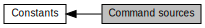
\includegraphics[width=277pt]{group__IL__CONST__CMD__SRC}
\end{center}
\end{figure}
\subsection*{Macros}
\begin{DoxyCompactItemize}
\item 
\#define \hyperlink{group__IL__CONST__CMD__SRC_ga88919277ef4cb64e612b18356061b87d}{I\+L\+K\+\_\+\+C\+M\+D\+\_\+\+S\+R\+C\+\_\+\+N\+E\+T\+W\+O\+RK}~0x00
\begin{DoxyCompactList}\small\item\em Network. \end{DoxyCompactList}\item 
\#define \hyperlink{group__IL__CONST__CMD__SRC_gaef878333a1356fde2b0534a169b93978}{I\+L\+K\+\_\+\+C\+M\+D\+\_\+\+S\+R\+C\+\_\+\+A\+IN}~0x01
\begin{DoxyCompactList}\small\item\em Analog input. \end{DoxyCompactList}\item 
\#define \hyperlink{group__IL__CONST__CMD__SRC_ga354c3281eb53b704f8fb7a6ec62a88c6}{I\+L\+K\+\_\+\+C\+M\+D\+\_\+\+S\+R\+C\+\_\+\+P\+WM}~0x02
\begin{DoxyCompactList}\small\item\em P\+WM or P\+WM \& direction. \end{DoxyCompactList}\item 
\#define \hyperlink{group__IL__CONST__CMD__SRC_ga65139db060bb9ccf75324070aac63635}{I\+L\+K\+\_\+\+C\+M\+D\+\_\+\+S\+R\+C\+\_\+\+S\+T\+E\+P\+D\+IR}~0x03
\begin{DoxyCompactList}\small\item\em Step \& direction. \end{DoxyCompactList}\item 
\#define \hyperlink{group__IL__CONST__CMD__SRC_ga23b5f07af7a7285c8e7cf0d371586f1d}{I\+L\+K\+\_\+\+C\+M\+D\+\_\+\+S\+R\+C\+\_\+\+E\+G\+E\+A\+R\+I\+NG}~0x05
\begin{DoxyCompactList}\small\item\em Electronic gearing. \end{DoxyCompactList}\item 
\#define \hyperlink{group__IL__CONST__CMD__SRC_gaf24cb62945a45167b7edb440559baab4}{I\+L\+K\+\_\+\+C\+M\+D\+\_\+\+S\+R\+C\+\_\+\+I\+N\+T\+E\+G\+R\+A\+L\+\_\+\+G\+EN}~0x06
\begin{DoxyCompactList}\small\item\em Integral generator. \end{DoxyCompactList}\end{DoxyCompactItemize}


\subsection{Detailed Description}


\subsection{Macro Definition Documentation}
\index{Command sources@{Command sources}!I\+L\+K\+\_\+\+C\+M\+D\+\_\+\+S\+R\+C\+\_\+\+A\+IN@{I\+L\+K\+\_\+\+C\+M\+D\+\_\+\+S\+R\+C\+\_\+\+A\+IN}}
\index{I\+L\+K\+\_\+\+C\+M\+D\+\_\+\+S\+R\+C\+\_\+\+A\+IN@{I\+L\+K\+\_\+\+C\+M\+D\+\_\+\+S\+R\+C\+\_\+\+A\+IN}!Command sources@{Command sources}}
\subsubsection[{\texorpdfstring{I\+L\+K\+\_\+\+C\+M\+D\+\_\+\+S\+R\+C\+\_\+\+A\+IN}{ILK_CMD_SRC_AIN}}]{\setlength{\rightskip}{0pt plus 5cm}\#define I\+L\+K\+\_\+\+C\+M\+D\+\_\+\+S\+R\+C\+\_\+\+A\+IN~0x01}\hypertarget{group__IL__CONST__CMD__SRC_gaef878333a1356fde2b0534a169b93978}{}\label{group__IL__CONST__CMD__SRC_gaef878333a1356fde2b0534a169b93978}


Analog input. 

\index{Command sources@{Command sources}!I\+L\+K\+\_\+\+C\+M\+D\+\_\+\+S\+R\+C\+\_\+\+E\+G\+E\+A\+R\+I\+NG@{I\+L\+K\+\_\+\+C\+M\+D\+\_\+\+S\+R\+C\+\_\+\+E\+G\+E\+A\+R\+I\+NG}}
\index{I\+L\+K\+\_\+\+C\+M\+D\+\_\+\+S\+R\+C\+\_\+\+E\+G\+E\+A\+R\+I\+NG@{I\+L\+K\+\_\+\+C\+M\+D\+\_\+\+S\+R\+C\+\_\+\+E\+G\+E\+A\+R\+I\+NG}!Command sources@{Command sources}}
\subsubsection[{\texorpdfstring{I\+L\+K\+\_\+\+C\+M\+D\+\_\+\+S\+R\+C\+\_\+\+E\+G\+E\+A\+R\+I\+NG}{ILK_CMD_SRC_EGEARING}}]{\setlength{\rightskip}{0pt plus 5cm}\#define I\+L\+K\+\_\+\+C\+M\+D\+\_\+\+S\+R\+C\+\_\+\+E\+G\+E\+A\+R\+I\+NG~0x05}\hypertarget{group__IL__CONST__CMD__SRC_ga23b5f07af7a7285c8e7cf0d371586f1d}{}\label{group__IL__CONST__CMD__SRC_ga23b5f07af7a7285c8e7cf0d371586f1d}


Electronic gearing. 

\index{Command sources@{Command sources}!I\+L\+K\+\_\+\+C\+M\+D\+\_\+\+S\+R\+C\+\_\+\+I\+N\+T\+E\+G\+R\+A\+L\+\_\+\+G\+EN@{I\+L\+K\+\_\+\+C\+M\+D\+\_\+\+S\+R\+C\+\_\+\+I\+N\+T\+E\+G\+R\+A\+L\+\_\+\+G\+EN}}
\index{I\+L\+K\+\_\+\+C\+M\+D\+\_\+\+S\+R\+C\+\_\+\+I\+N\+T\+E\+G\+R\+A\+L\+\_\+\+G\+EN@{I\+L\+K\+\_\+\+C\+M\+D\+\_\+\+S\+R\+C\+\_\+\+I\+N\+T\+E\+G\+R\+A\+L\+\_\+\+G\+EN}!Command sources@{Command sources}}
\subsubsection[{\texorpdfstring{I\+L\+K\+\_\+\+C\+M\+D\+\_\+\+S\+R\+C\+\_\+\+I\+N\+T\+E\+G\+R\+A\+L\+\_\+\+G\+EN}{ILK_CMD_SRC_INTEGRAL_GEN}}]{\setlength{\rightskip}{0pt plus 5cm}\#define I\+L\+K\+\_\+\+C\+M\+D\+\_\+\+S\+R\+C\+\_\+\+I\+N\+T\+E\+G\+R\+A\+L\+\_\+\+G\+EN~0x06}\hypertarget{group__IL__CONST__CMD__SRC_gaf24cb62945a45167b7edb440559baab4}{}\label{group__IL__CONST__CMD__SRC_gaf24cb62945a45167b7edb440559baab4}


Integral generator. 

\index{Command sources@{Command sources}!I\+L\+K\+\_\+\+C\+M\+D\+\_\+\+S\+R\+C\+\_\+\+N\+E\+T\+W\+O\+RK@{I\+L\+K\+\_\+\+C\+M\+D\+\_\+\+S\+R\+C\+\_\+\+N\+E\+T\+W\+O\+RK}}
\index{I\+L\+K\+\_\+\+C\+M\+D\+\_\+\+S\+R\+C\+\_\+\+N\+E\+T\+W\+O\+RK@{I\+L\+K\+\_\+\+C\+M\+D\+\_\+\+S\+R\+C\+\_\+\+N\+E\+T\+W\+O\+RK}!Command sources@{Command sources}}
\subsubsection[{\texorpdfstring{I\+L\+K\+\_\+\+C\+M\+D\+\_\+\+S\+R\+C\+\_\+\+N\+E\+T\+W\+O\+RK}{ILK_CMD_SRC_NETWORK}}]{\setlength{\rightskip}{0pt plus 5cm}\#define I\+L\+K\+\_\+\+C\+M\+D\+\_\+\+S\+R\+C\+\_\+\+N\+E\+T\+W\+O\+RK~0x00}\hypertarget{group__IL__CONST__CMD__SRC_ga88919277ef4cb64e612b18356061b87d}{}\label{group__IL__CONST__CMD__SRC_ga88919277ef4cb64e612b18356061b87d}


Network. 

\index{Command sources@{Command sources}!I\+L\+K\+\_\+\+C\+M\+D\+\_\+\+S\+R\+C\+\_\+\+P\+WM@{I\+L\+K\+\_\+\+C\+M\+D\+\_\+\+S\+R\+C\+\_\+\+P\+WM}}
\index{I\+L\+K\+\_\+\+C\+M\+D\+\_\+\+S\+R\+C\+\_\+\+P\+WM@{I\+L\+K\+\_\+\+C\+M\+D\+\_\+\+S\+R\+C\+\_\+\+P\+WM}!Command sources@{Command sources}}
\subsubsection[{\texorpdfstring{I\+L\+K\+\_\+\+C\+M\+D\+\_\+\+S\+R\+C\+\_\+\+P\+WM}{ILK_CMD_SRC_PWM}}]{\setlength{\rightskip}{0pt plus 5cm}\#define I\+L\+K\+\_\+\+C\+M\+D\+\_\+\+S\+R\+C\+\_\+\+P\+WM~0x02}\hypertarget{group__IL__CONST__CMD__SRC_ga354c3281eb53b704f8fb7a6ec62a88c6}{}\label{group__IL__CONST__CMD__SRC_ga354c3281eb53b704f8fb7a6ec62a88c6}


P\+WM or P\+WM \& direction. 

\index{Command sources@{Command sources}!I\+L\+K\+\_\+\+C\+M\+D\+\_\+\+S\+R\+C\+\_\+\+S\+T\+E\+P\+D\+IR@{I\+L\+K\+\_\+\+C\+M\+D\+\_\+\+S\+R\+C\+\_\+\+S\+T\+E\+P\+D\+IR}}
\index{I\+L\+K\+\_\+\+C\+M\+D\+\_\+\+S\+R\+C\+\_\+\+S\+T\+E\+P\+D\+IR@{I\+L\+K\+\_\+\+C\+M\+D\+\_\+\+S\+R\+C\+\_\+\+S\+T\+E\+P\+D\+IR}!Command sources@{Command sources}}
\subsubsection[{\texorpdfstring{I\+L\+K\+\_\+\+C\+M\+D\+\_\+\+S\+R\+C\+\_\+\+S\+T\+E\+P\+D\+IR}{ILK_CMD_SRC_STEPDIR}}]{\setlength{\rightskip}{0pt plus 5cm}\#define I\+L\+K\+\_\+\+C\+M\+D\+\_\+\+S\+R\+C\+\_\+\+S\+T\+E\+P\+D\+IR~0x03}\hypertarget{group__IL__CONST__CMD__SRC_ga65139db060bb9ccf75324070aac63635}{}\label{group__IL__CONST__CMD__SRC_ga65139db060bb9ccf75324070aac63635}


Step \& direction. 


\hypertarget{group__IL__DICT}{}\section{Dictionary}
\label{group__IL__DICT}\index{Dictionary@{Dictionary}}
Collaboration diagram for Dictionary\+:\nopagebreak
\begin{figure}[H]
\begin{center}
\leavevmode
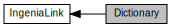
\includegraphics[width=243pt]{group__IL__DICT}
\end{center}
\end{figure}
\subsection*{Typedefs}
\begin{DoxyCompactItemize}
\item 
typedef struct il\+\_\+dict \hyperlink{group__IL__DICT_gac2cb8ba7974d8506df3017879572fc84}{il\+\_\+dict\+\_\+t}
\begin{DoxyCompactList}\small\item\em Ingenia\+Link dictionary. \end{DoxyCompactList}\end{DoxyCompactItemize}
\subsection*{Functions}
\begin{DoxyCompactItemize}
\item 
\hyperlink{common_8h_a6bb629d26c52bfe10519ba3176853f47}{I\+L\+\_\+\+E\+X\+P\+O\+RT} \hyperlink{group__IL__DICT_gac2cb8ba7974d8506df3017879572fc84}{il\+\_\+dict\+\_\+t} $\ast$ \hyperlink{group__IL__DICT_gaf3d1da6ffb1d4efcf40946dc705230f2}{il\+\_\+dict\+\_\+create} (const char $\ast$dict\+\_\+f)
\begin{DoxyCompactList}\small\item\em Create a dictionary. \end{DoxyCompactList}\item 
\hyperlink{common_8h_a6bb629d26c52bfe10519ba3176853f47}{I\+L\+\_\+\+E\+X\+P\+O\+RT} void \hyperlink{group__IL__DICT_ga37cc4ceb38514581a5bbecb47f5cfa61}{il\+\_\+dict\+\_\+destroy} (\hyperlink{group__IL__DICT_gac2cb8ba7974d8506df3017879572fc84}{il\+\_\+dict\+\_\+t} $\ast$dict)
\begin{DoxyCompactList}\small\item\em Destroy a dictionary. \end{DoxyCompactList}\item 
\hyperlink{common_8h_a6bb629d26c52bfe10519ba3176853f47}{I\+L\+\_\+\+E\+X\+P\+O\+RT} int \hyperlink{group__IL__DICT_ga3ea660af3316835c1799ce8dca67b566}{il\+\_\+dict\+\_\+cat\+\_\+get} (\hyperlink{group__IL__DICT_gac2cb8ba7974d8506df3017879572fc84}{il\+\_\+dict\+\_\+t} $\ast$dict, const char $\ast$cat\+\_\+id, \hyperlink{group__IL__DICT__LABELS_ga69d1109256f465cbcfa8aac7fa592495}{il\+\_\+dict\+\_\+labels\+\_\+t} $\ast$$\ast$labels)
\begin{DoxyCompactList}\small\item\em Obtain category labels from ID. \end{DoxyCompactList}\item 
\hyperlink{common_8h_a6bb629d26c52bfe10519ba3176853f47}{I\+L\+\_\+\+E\+X\+P\+O\+RT} size\+\_\+t \hyperlink{group__IL__DICT_gac982efe51c1ceca824b89b729397bf6f}{il\+\_\+dict\+\_\+cat\+\_\+cnt} (\hyperlink{group__IL__DICT_gac2cb8ba7974d8506df3017879572fc84}{il\+\_\+dict\+\_\+t} $\ast$dict)
\begin{DoxyCompactList}\small\item\em Obtain number of categories in the dictionary. \end{DoxyCompactList}\item 
\hyperlink{common_8h_a6bb629d26c52bfe10519ba3176853f47}{I\+L\+\_\+\+E\+X\+P\+O\+RT} const char $\ast$$\ast$ \hyperlink{group__IL__DICT_ga254bc46b2740b8291fd0061e47c28758}{il\+\_\+dict\+\_\+cat\+\_\+ids\+\_\+get} (\hyperlink{group__IL__DICT_gac2cb8ba7974d8506df3017879572fc84}{il\+\_\+dict\+\_\+t} $\ast$dict)
\begin{DoxyCompactList}\small\item\em Obtain the list of category I\+Ds. \end{DoxyCompactList}\item 
\hyperlink{common_8h_a6bb629d26c52bfe10519ba3176853f47}{I\+L\+\_\+\+E\+X\+P\+O\+RT} void \hyperlink{group__IL__DICT_ga27125d99f6aa90dc36c3de0736993265}{il\+\_\+dict\+\_\+cat\+\_\+ids\+\_\+destroy} (const char $\ast$$\ast$cat\+\_\+ids)
\begin{DoxyCompactList}\small\item\em Destroy the list of obtained category I\+Ds. \end{DoxyCompactList}\item 
\hyperlink{common_8h_a6bb629d26c52bfe10519ba3176853f47}{I\+L\+\_\+\+E\+X\+P\+O\+RT} int \hyperlink{group__IL__DICT_ga79fb4bf5b1fab3d67a201c6e5b11e5e7}{il\+\_\+dict\+\_\+scat\+\_\+get} (\hyperlink{group__IL__DICT_gac2cb8ba7974d8506df3017879572fc84}{il\+\_\+dict\+\_\+t} $\ast$dict, const char $\ast$cat\+\_\+id, const char $\ast$scat\+\_\+id, \hyperlink{group__IL__DICT__LABELS_ga69d1109256f465cbcfa8aac7fa592495}{il\+\_\+dict\+\_\+labels\+\_\+t} $\ast$$\ast$labels)
\begin{DoxyCompactList}\small\item\em Obtain sub-\/category labels from a category. \end{DoxyCompactList}\item 
\hyperlink{common_8h_a6bb629d26c52bfe10519ba3176853f47}{I\+L\+\_\+\+E\+X\+P\+O\+RT} size\+\_\+t \hyperlink{group__IL__DICT_gac34ec4d95d8526d1cf09641c843ce7aa}{il\+\_\+dict\+\_\+scat\+\_\+cnt} (\hyperlink{group__IL__DICT_gac2cb8ba7974d8506df3017879572fc84}{il\+\_\+dict\+\_\+t} $\ast$dict, const char $\ast$cat\+\_\+id)
\begin{DoxyCompactList}\small\item\em Obtain number of sub-\/categories in a category. \end{DoxyCompactList}\item 
\hyperlink{common_8h_a6bb629d26c52bfe10519ba3176853f47}{I\+L\+\_\+\+E\+X\+P\+O\+RT} const char $\ast$$\ast$ \hyperlink{group__IL__DICT_ga51782d1acdcfd574ab717c6c721cb560}{il\+\_\+dict\+\_\+scat\+\_\+ids\+\_\+get} (\hyperlink{group__IL__DICT_gac2cb8ba7974d8506df3017879572fc84}{il\+\_\+dict\+\_\+t} $\ast$dict, const char $\ast$cat\+\_\+id)
\begin{DoxyCompactList}\small\item\em Obtain the list of category I\+Ds. \end{DoxyCompactList}\item 
\hyperlink{common_8h_a6bb629d26c52bfe10519ba3176853f47}{I\+L\+\_\+\+E\+X\+P\+O\+RT} void \hyperlink{group__IL__DICT_gaa558e902f07600780b351f9e58f443df}{il\+\_\+dict\+\_\+scat\+\_\+ids\+\_\+destroy} (const char $\ast$$\ast$scat\+\_\+ids)
\begin{DoxyCompactList}\small\item\em Destroy the list of obtained sub-\/category I\+Ds. \end{DoxyCompactList}\item 
\hyperlink{common_8h_a6bb629d26c52bfe10519ba3176853f47}{I\+L\+\_\+\+E\+X\+P\+O\+RT} int \hyperlink{group__IL__DICT_ga2c1e206d3c5d57a4a047855c2743fa5a}{il\+\_\+dict\+\_\+reg\+\_\+get} (\hyperlink{group__IL__DICT_gac2cb8ba7974d8506df3017879572fc84}{il\+\_\+dict\+\_\+t} $\ast$dict, const char $\ast$id, const \hyperlink{structil__reg__t}{il\+\_\+reg\+\_\+t} $\ast$$\ast$reg)
\begin{DoxyCompactList}\small\item\em Obtain register from ID. \end{DoxyCompactList}\item 
\hyperlink{common_8h_a6bb629d26c52bfe10519ba3176853f47}{I\+L\+\_\+\+E\+X\+P\+O\+RT} size\+\_\+t \hyperlink{group__IL__DICT_ga7d1b8cad25b75ec725c9dad237fe918a}{il\+\_\+dict\+\_\+reg\+\_\+cnt} (\hyperlink{group__IL__DICT_gac2cb8ba7974d8506df3017879572fc84}{il\+\_\+dict\+\_\+t} $\ast$dict)
\begin{DoxyCompactList}\small\item\em Obtain number of registers in the dictionary. \end{DoxyCompactList}\item 
\hyperlink{common_8h_a6bb629d26c52bfe10519ba3176853f47}{I\+L\+\_\+\+E\+X\+P\+O\+RT} const char $\ast$$\ast$ \hyperlink{group__IL__DICT_gaaf93ee11fe3006f72c03f03174abdf33}{il\+\_\+dict\+\_\+reg\+\_\+ids\+\_\+get} (\hyperlink{group__IL__DICT_gac2cb8ba7974d8506df3017879572fc84}{il\+\_\+dict\+\_\+t} $\ast$dict)
\begin{DoxyCompactList}\small\item\em Obtain the list of register I\+Ds. \end{DoxyCompactList}\item 
\hyperlink{common_8h_a6bb629d26c52bfe10519ba3176853f47}{I\+L\+\_\+\+E\+X\+P\+O\+RT} void \hyperlink{group__IL__DICT_gacd7922e14cb903f3342747ed21a00ec1}{il\+\_\+dict\+\_\+reg\+\_\+ids\+\_\+destroy} (const char $\ast$$\ast$regs)
\begin{DoxyCompactList}\small\item\em Destroy the list of obtained register I\+Ds. \end{DoxyCompactList}\end{DoxyCompactItemize}


\subsection{Detailed Description}


\subsection{Typedef Documentation}
\index{Dictionary@{Dictionary}!il\+\_\+dict\+\_\+t@{il\+\_\+dict\+\_\+t}}
\index{il\+\_\+dict\+\_\+t@{il\+\_\+dict\+\_\+t}!Dictionary@{Dictionary}}
\subsubsection[{\texorpdfstring{il\+\_\+dict\+\_\+t}{il_dict_t}}]{\setlength{\rightskip}{0pt plus 5cm}typedef struct il\+\_\+dict {\bf il\+\_\+dict\+\_\+t}}\hypertarget{group__IL__DICT_gac2cb8ba7974d8506df3017879572fc84}{}\label{group__IL__DICT_gac2cb8ba7974d8506df3017879572fc84}


Ingenia\+Link dictionary. 



\subsection{Function Documentation}
\index{Dictionary@{Dictionary}!il\+\_\+dict\+\_\+cat\+\_\+cnt@{il\+\_\+dict\+\_\+cat\+\_\+cnt}}
\index{il\+\_\+dict\+\_\+cat\+\_\+cnt@{il\+\_\+dict\+\_\+cat\+\_\+cnt}!Dictionary@{Dictionary}}
\subsubsection[{\texorpdfstring{il\+\_\+dict\+\_\+cat\+\_\+cnt(il\+\_\+dict\+\_\+t $\ast$dict)}{il_dict_cat_cnt(il_dict_t *dict)}}]{\setlength{\rightskip}{0pt plus 5cm}{\bf I\+L\+\_\+\+E\+X\+P\+O\+RT} size\+\_\+t il\+\_\+dict\+\_\+cat\+\_\+cnt (
\begin{DoxyParamCaption}
\item[{{\bf il\+\_\+dict\+\_\+t} $\ast$}]{dict}
\end{DoxyParamCaption}
)}\hypertarget{group__IL__DICT_gac982efe51c1ceca824b89b729397bf6f}{}\label{group__IL__DICT_gac982efe51c1ceca824b89b729397bf6f}


Obtain number of categories in the dictionary. 


\begin{DoxyParams}[1]{Parameters}
\mbox{\tt in}  & {\em dict} & Dictionary instance.\\
\hline
\end{DoxyParams}
\begin{DoxyReturn}{Returns}
Number of categories in the dictionary. 
\end{DoxyReturn}
\index{Dictionary@{Dictionary}!il\+\_\+dict\+\_\+cat\+\_\+get@{il\+\_\+dict\+\_\+cat\+\_\+get}}
\index{il\+\_\+dict\+\_\+cat\+\_\+get@{il\+\_\+dict\+\_\+cat\+\_\+get}!Dictionary@{Dictionary}}
\subsubsection[{\texorpdfstring{il\+\_\+dict\+\_\+cat\+\_\+get(il\+\_\+dict\+\_\+t $\ast$dict, const char $\ast$cat\+\_\+id, il\+\_\+dict\+\_\+labels\+\_\+t $\ast$$\ast$labels)}{il_dict_cat_get(il_dict_t *dict, const char *cat_id, il_dict_labels_t **labels)}}]{\setlength{\rightskip}{0pt plus 5cm}{\bf I\+L\+\_\+\+E\+X\+P\+O\+RT} int il\+\_\+dict\+\_\+cat\+\_\+get (
\begin{DoxyParamCaption}
\item[{{\bf il\+\_\+dict\+\_\+t} $\ast$}]{dict, }
\item[{const char $\ast$}]{cat\+\_\+id, }
\item[{{\bf il\+\_\+dict\+\_\+labels\+\_\+t} $\ast$$\ast$}]{labels}
\end{DoxyParamCaption}
)}\hypertarget{group__IL__DICT_ga3ea660af3316835c1799ce8dca67b566}{}\label{group__IL__DICT_ga3ea660af3316835c1799ce8dca67b566}


Obtain category labels from ID. 


\begin{DoxyParams}[1]{Parameters}
\mbox{\tt in}  & {\em dict} & Dictionary instance. \\
\hline
\mbox{\tt in}  & {\em cat\+\_\+id} & Category ID. \\
\hline
\mbox{\tt out}  & {\em labels} & Where labels for the given ID will be stored.\\
\hline
\end{DoxyParams}
\begin{DoxyReturn}{Returns}
0 on success, I\+L\+\_\+\+E\+F\+A\+IL if the register does not exist. 
\end{DoxyReturn}
\begin{Desc}
\item[Examples\+: ]\par
\hyperlink{dict_8c-example}{dict.\+c}.\end{Desc}
\index{Dictionary@{Dictionary}!il\+\_\+dict\+\_\+cat\+\_\+ids\+\_\+destroy@{il\+\_\+dict\+\_\+cat\+\_\+ids\+\_\+destroy}}
\index{il\+\_\+dict\+\_\+cat\+\_\+ids\+\_\+destroy@{il\+\_\+dict\+\_\+cat\+\_\+ids\+\_\+destroy}!Dictionary@{Dictionary}}
\subsubsection[{\texorpdfstring{il\+\_\+dict\+\_\+cat\+\_\+ids\+\_\+destroy(const char $\ast$$\ast$cat\+\_\+ids)}{il_dict_cat_ids_destroy(const char **cat_ids)}}]{\setlength{\rightskip}{0pt plus 5cm}{\bf I\+L\+\_\+\+E\+X\+P\+O\+RT} void il\+\_\+dict\+\_\+cat\+\_\+ids\+\_\+destroy (
\begin{DoxyParamCaption}
\item[{const char $\ast$$\ast$}]{cat\+\_\+ids}
\end{DoxyParamCaption}
)}\hypertarget{group__IL__DICT_ga27125d99f6aa90dc36c3de0736993265}{}\label{group__IL__DICT_ga27125d99f6aa90dc36c3de0736993265}


Destroy the list of obtained category I\+Ds. 


\begin{DoxyParams}[1]{Parameters}
\mbox{\tt in}  & {\em cat\+\_\+ids} & Categories I\+Ds.\\
\hline
\end{DoxyParams}
\begin{DoxySeeAlso}{See also}
\hyperlink{group__IL__DICT_ga254bc46b2740b8291fd0061e47c28758}{il\+\_\+dict\+\_\+cat\+\_\+ids\+\_\+get} 
\end{DoxySeeAlso}
\begin{Desc}
\item[Examples\+: ]\par
\hyperlink{dict_8c-example}{dict.\+c}.\end{Desc}
\index{Dictionary@{Dictionary}!il\+\_\+dict\+\_\+cat\+\_\+ids\+\_\+get@{il\+\_\+dict\+\_\+cat\+\_\+ids\+\_\+get}}
\index{il\+\_\+dict\+\_\+cat\+\_\+ids\+\_\+get@{il\+\_\+dict\+\_\+cat\+\_\+ids\+\_\+get}!Dictionary@{Dictionary}}
\subsubsection[{\texorpdfstring{il\+\_\+dict\+\_\+cat\+\_\+ids\+\_\+get(il\+\_\+dict\+\_\+t $\ast$dict)}{il_dict_cat_ids_get(il_dict_t *dict)}}]{\setlength{\rightskip}{0pt plus 5cm}{\bf I\+L\+\_\+\+E\+X\+P\+O\+RT} const char$\ast$$\ast$ il\+\_\+dict\+\_\+cat\+\_\+ids\+\_\+get (
\begin{DoxyParamCaption}
\item[{{\bf il\+\_\+dict\+\_\+t} $\ast$}]{dict}
\end{DoxyParamCaption}
)}\hypertarget{group__IL__DICT_ga254bc46b2740b8291fd0061e47c28758}{}\label{group__IL__DICT_ga254bc46b2740b8291fd0061e47c28758}


Obtain the list of category I\+Ds. 


\begin{DoxyParams}[1]{Parameters}
\mbox{\tt in}  & {\em dict} & Dictionary instance.\\
\hline
\end{DoxyParams}
\begin{DoxyReturn}{Returns}
Category I\+Ds (N\+U\+LL if none or error).
\end{DoxyReturn}
\begin{DoxySeeAlso}{See also}
\hyperlink{group__IL__DICT_ga27125d99f6aa90dc36c3de0736993265}{il\+\_\+dict\+\_\+cat\+\_\+ids\+\_\+destroy} 
\end{DoxySeeAlso}
\begin{Desc}
\item[Examples\+: ]\par
\hyperlink{dict_8c-example}{dict.\+c}.\end{Desc}
\index{Dictionary@{Dictionary}!il\+\_\+dict\+\_\+create@{il\+\_\+dict\+\_\+create}}
\index{il\+\_\+dict\+\_\+create@{il\+\_\+dict\+\_\+create}!Dictionary@{Dictionary}}
\subsubsection[{\texorpdfstring{il\+\_\+dict\+\_\+create(const char $\ast$dict\+\_\+f)}{il_dict_create(const char *dict_f)}}]{\setlength{\rightskip}{0pt plus 5cm}{\bf I\+L\+\_\+\+E\+X\+P\+O\+RT} {\bf il\+\_\+dict\+\_\+t}$\ast$ il\+\_\+dict\+\_\+create (
\begin{DoxyParamCaption}
\item[{const char $\ast$}]{dict\+\_\+f}
\end{DoxyParamCaption}
)}\hypertarget{group__IL__DICT_gaf3d1da6ffb1d4efcf40946dc705230f2}{}\label{group__IL__DICT_gaf3d1da6ffb1d4efcf40946dc705230f2}


Create a dictionary. 


\begin{DoxyParams}[1]{Parameters}
\mbox{\tt in}  & {\em dict\+\_\+f} & Dictionary file.\\
\hline
\end{DoxyParams}
\begin{DoxyReturn}{Returns}
Dictionary instance. 
\end{DoxyReturn}
\begin{Desc}
\item[Examples\+: ]\par
\hyperlink{dict_8c-example}{dict.\+c}.\end{Desc}
\index{Dictionary@{Dictionary}!il\+\_\+dict\+\_\+destroy@{il\+\_\+dict\+\_\+destroy}}
\index{il\+\_\+dict\+\_\+destroy@{il\+\_\+dict\+\_\+destroy}!Dictionary@{Dictionary}}
\subsubsection[{\texorpdfstring{il\+\_\+dict\+\_\+destroy(il\+\_\+dict\+\_\+t $\ast$dict)}{il_dict_destroy(il_dict_t *dict)}}]{\setlength{\rightskip}{0pt plus 5cm}{\bf I\+L\+\_\+\+E\+X\+P\+O\+RT} void il\+\_\+dict\+\_\+destroy (
\begin{DoxyParamCaption}
\item[{{\bf il\+\_\+dict\+\_\+t} $\ast$}]{dict}
\end{DoxyParamCaption}
)}\hypertarget{group__IL__DICT_ga37cc4ceb38514581a5bbecb47f5cfa61}{}\label{group__IL__DICT_ga37cc4ceb38514581a5bbecb47f5cfa61}


Destroy a dictionary. 


\begin{DoxyParams}[1]{Parameters}
\mbox{\tt in,out}  & {\em dict} & Dictionary instance. \\
\hline
\end{DoxyParams}
\begin{Desc}
\item[Examples\+: ]\par
\hyperlink{dict_8c-example}{dict.\+c}.\end{Desc}
\index{Dictionary@{Dictionary}!il\+\_\+dict\+\_\+reg\+\_\+cnt@{il\+\_\+dict\+\_\+reg\+\_\+cnt}}
\index{il\+\_\+dict\+\_\+reg\+\_\+cnt@{il\+\_\+dict\+\_\+reg\+\_\+cnt}!Dictionary@{Dictionary}}
\subsubsection[{\texorpdfstring{il\+\_\+dict\+\_\+reg\+\_\+cnt(il\+\_\+dict\+\_\+t $\ast$dict)}{il_dict_reg_cnt(il_dict_t *dict)}}]{\setlength{\rightskip}{0pt plus 5cm}{\bf I\+L\+\_\+\+E\+X\+P\+O\+RT} size\+\_\+t il\+\_\+dict\+\_\+reg\+\_\+cnt (
\begin{DoxyParamCaption}
\item[{{\bf il\+\_\+dict\+\_\+t} $\ast$}]{dict}
\end{DoxyParamCaption}
)}\hypertarget{group__IL__DICT_ga7d1b8cad25b75ec725c9dad237fe918a}{}\label{group__IL__DICT_ga7d1b8cad25b75ec725c9dad237fe918a}


Obtain number of registers in the dictionary. 


\begin{DoxyParams}[1]{Parameters}
\mbox{\tt in}  & {\em dict} & Dictionary instance.\\
\hline
\end{DoxyParams}
\begin{DoxyReturn}{Returns}
Number of registers in the dictionary. 
\end{DoxyReturn}
\index{Dictionary@{Dictionary}!il\+\_\+dict\+\_\+reg\+\_\+get@{il\+\_\+dict\+\_\+reg\+\_\+get}}
\index{il\+\_\+dict\+\_\+reg\+\_\+get@{il\+\_\+dict\+\_\+reg\+\_\+get}!Dictionary@{Dictionary}}
\subsubsection[{\texorpdfstring{il\+\_\+dict\+\_\+reg\+\_\+get(il\+\_\+dict\+\_\+t $\ast$dict, const char $\ast$id, const il\+\_\+reg\+\_\+t $\ast$$\ast$reg)}{il_dict_reg_get(il_dict_t *dict, const char *id, const il_reg_t **reg)}}]{\setlength{\rightskip}{0pt plus 5cm}{\bf I\+L\+\_\+\+E\+X\+P\+O\+RT} int il\+\_\+dict\+\_\+reg\+\_\+get (
\begin{DoxyParamCaption}
\item[{{\bf il\+\_\+dict\+\_\+t} $\ast$}]{dict, }
\item[{const char $\ast$}]{id, }
\item[{const {\bf il\+\_\+reg\+\_\+t} $\ast$$\ast$}]{reg}
\end{DoxyParamCaption}
)}\hypertarget{group__IL__DICT_ga2c1e206d3c5d57a4a047855c2743fa5a}{}\label{group__IL__DICT_ga2c1e206d3c5d57a4a047855c2743fa5a}


Obtain register from ID. 


\begin{DoxyParams}[1]{Parameters}
\mbox{\tt in}  & {\em dict} & Dictionary instance. \\
\hline
\mbox{\tt in}  & {\em id} & Register ID. \\
\hline
\mbox{\tt out}  & {\em reg} & Where register with given ID will be stored.\\
\hline
\end{DoxyParams}
\begin{DoxyReturn}{Returns}
0 on success, I\+L\+\_\+\+E\+F\+A\+IL if the register does not exist. 
\end{DoxyReturn}
\begin{Desc}
\item[Examples\+: ]\par
\hyperlink{dict_8c-example}{dict.\+c}.\end{Desc}
\index{Dictionary@{Dictionary}!il\+\_\+dict\+\_\+reg\+\_\+ids\+\_\+destroy@{il\+\_\+dict\+\_\+reg\+\_\+ids\+\_\+destroy}}
\index{il\+\_\+dict\+\_\+reg\+\_\+ids\+\_\+destroy@{il\+\_\+dict\+\_\+reg\+\_\+ids\+\_\+destroy}!Dictionary@{Dictionary}}
\subsubsection[{\texorpdfstring{il\+\_\+dict\+\_\+reg\+\_\+ids\+\_\+destroy(const char $\ast$$\ast$regs)}{il_dict_reg_ids_destroy(const char **regs)}}]{\setlength{\rightskip}{0pt plus 5cm}{\bf I\+L\+\_\+\+E\+X\+P\+O\+RT} void il\+\_\+dict\+\_\+reg\+\_\+ids\+\_\+destroy (
\begin{DoxyParamCaption}
\item[{const char $\ast$$\ast$}]{regs}
\end{DoxyParamCaption}
)}\hypertarget{group__IL__DICT_gacd7922e14cb903f3342747ed21a00ec1}{}\label{group__IL__DICT_gacd7922e14cb903f3342747ed21a00ec1}


Destroy the list of obtained register I\+Ds. 


\begin{DoxyParams}[1]{Parameters}
\mbox{\tt in}  & {\em regs} & Register list.\\
\hline
\end{DoxyParams}
\begin{DoxySeeAlso}{See also}
\hyperlink{group__IL__DICT_gaaf93ee11fe3006f72c03f03174abdf33}{il\+\_\+dict\+\_\+reg\+\_\+ids\+\_\+get} 
\end{DoxySeeAlso}
\begin{Desc}
\item[Examples\+: ]\par
\hyperlink{dict_8c-example}{dict.\+c}.\end{Desc}
\index{Dictionary@{Dictionary}!il\+\_\+dict\+\_\+reg\+\_\+ids\+\_\+get@{il\+\_\+dict\+\_\+reg\+\_\+ids\+\_\+get}}
\index{il\+\_\+dict\+\_\+reg\+\_\+ids\+\_\+get@{il\+\_\+dict\+\_\+reg\+\_\+ids\+\_\+get}!Dictionary@{Dictionary}}
\subsubsection[{\texorpdfstring{il\+\_\+dict\+\_\+reg\+\_\+ids\+\_\+get(il\+\_\+dict\+\_\+t $\ast$dict)}{il_dict_reg_ids_get(il_dict_t *dict)}}]{\setlength{\rightskip}{0pt plus 5cm}{\bf I\+L\+\_\+\+E\+X\+P\+O\+RT} const char$\ast$$\ast$ il\+\_\+dict\+\_\+reg\+\_\+ids\+\_\+get (
\begin{DoxyParamCaption}
\item[{{\bf il\+\_\+dict\+\_\+t} $\ast$}]{dict}
\end{DoxyParamCaption}
)}\hypertarget{group__IL__DICT_gaaf93ee11fe3006f72c03f03174abdf33}{}\label{group__IL__DICT_gaaf93ee11fe3006f72c03f03174abdf33}


Obtain the list of register I\+Ds. 


\begin{DoxyParams}[1]{Parameters}
\mbox{\tt in}  & {\em dict} & Dictionary instance.\\
\hline
\end{DoxyParams}
\begin{DoxyReturn}{Returns}
Dictionary I\+Ds (N\+U\+LL if none or error).
\end{DoxyReturn}
\begin{DoxySeeAlso}{See also}
\hyperlink{group__IL__DICT_gacd7922e14cb903f3342747ed21a00ec1}{il\+\_\+dict\+\_\+reg\+\_\+ids\+\_\+destroy} 
\end{DoxySeeAlso}
\begin{Desc}
\item[Examples\+: ]\par
\hyperlink{dict_8c-example}{dict.\+c}.\end{Desc}
\index{Dictionary@{Dictionary}!il\+\_\+dict\+\_\+scat\+\_\+cnt@{il\+\_\+dict\+\_\+scat\+\_\+cnt}}
\index{il\+\_\+dict\+\_\+scat\+\_\+cnt@{il\+\_\+dict\+\_\+scat\+\_\+cnt}!Dictionary@{Dictionary}}
\subsubsection[{\texorpdfstring{il\+\_\+dict\+\_\+scat\+\_\+cnt(il\+\_\+dict\+\_\+t $\ast$dict, const char $\ast$cat\+\_\+id)}{il_dict_scat_cnt(il_dict_t *dict, const char *cat_id)}}]{\setlength{\rightskip}{0pt plus 5cm}{\bf I\+L\+\_\+\+E\+X\+P\+O\+RT} size\+\_\+t il\+\_\+dict\+\_\+scat\+\_\+cnt (
\begin{DoxyParamCaption}
\item[{{\bf il\+\_\+dict\+\_\+t} $\ast$}]{dict, }
\item[{const char $\ast$}]{cat\+\_\+id}
\end{DoxyParamCaption}
)}\hypertarget{group__IL__DICT_gac34ec4d95d8526d1cf09641c843ce7aa}{}\label{group__IL__DICT_gac34ec4d95d8526d1cf09641c843ce7aa}


Obtain number of sub-\/categories in a category. 


\begin{DoxyParams}[1]{Parameters}
\mbox{\tt in}  & {\em dict} & Dictionary instance. \\
\hline
\mbox{\tt in}  & {\em cat\+\_\+id} & Category ID.\\
\hline
\end{DoxyParams}
\begin{DoxyReturn}{Returns}
Number of categories in the dictionary. 
\end{DoxyReturn}
\index{Dictionary@{Dictionary}!il\+\_\+dict\+\_\+scat\+\_\+get@{il\+\_\+dict\+\_\+scat\+\_\+get}}
\index{il\+\_\+dict\+\_\+scat\+\_\+get@{il\+\_\+dict\+\_\+scat\+\_\+get}!Dictionary@{Dictionary}}
\subsubsection[{\texorpdfstring{il\+\_\+dict\+\_\+scat\+\_\+get(il\+\_\+dict\+\_\+t $\ast$dict, const char $\ast$cat\+\_\+id, const char $\ast$scat\+\_\+id, il\+\_\+dict\+\_\+labels\+\_\+t $\ast$$\ast$labels)}{il_dict_scat_get(il_dict_t *dict, const char *cat_id, const char *scat_id, il_dict_labels_t **labels)}}]{\setlength{\rightskip}{0pt plus 5cm}{\bf I\+L\+\_\+\+E\+X\+P\+O\+RT} int il\+\_\+dict\+\_\+scat\+\_\+get (
\begin{DoxyParamCaption}
\item[{{\bf il\+\_\+dict\+\_\+t} $\ast$}]{dict, }
\item[{const char $\ast$}]{cat\+\_\+id, }
\item[{const char $\ast$}]{scat\+\_\+id, }
\item[{{\bf il\+\_\+dict\+\_\+labels\+\_\+t} $\ast$$\ast$}]{labels}
\end{DoxyParamCaption}
)}\hypertarget{group__IL__DICT_ga79fb4bf5b1fab3d67a201c6e5b11e5e7}{}\label{group__IL__DICT_ga79fb4bf5b1fab3d67a201c6e5b11e5e7}


Obtain sub-\/category labels from a category. 


\begin{DoxyParams}[1]{Parameters}
\mbox{\tt in}  & {\em dict} & Dictionary instance. \\
\hline
\mbox{\tt in}  & {\em cat\+\_\+id} & Category ID. \\
\hline
\mbox{\tt in}  & {\em scat\+\_\+id} & Sub-\/category ID. \\
\hline
\mbox{\tt out}  & {\em labels} & Where labels for the given ID will be stored.\\
\hline
\end{DoxyParams}
\begin{DoxyReturn}{Returns}
0 on success, I\+L\+\_\+\+E\+F\+A\+IL if the register does not exist. 
\end{DoxyReturn}
\begin{Desc}
\item[Examples\+: ]\par
\hyperlink{dict_8c-example}{dict.\+c}.\end{Desc}
\index{Dictionary@{Dictionary}!il\+\_\+dict\+\_\+scat\+\_\+ids\+\_\+destroy@{il\+\_\+dict\+\_\+scat\+\_\+ids\+\_\+destroy}}
\index{il\+\_\+dict\+\_\+scat\+\_\+ids\+\_\+destroy@{il\+\_\+dict\+\_\+scat\+\_\+ids\+\_\+destroy}!Dictionary@{Dictionary}}
\subsubsection[{\texorpdfstring{il\+\_\+dict\+\_\+scat\+\_\+ids\+\_\+destroy(const char $\ast$$\ast$scat\+\_\+ids)}{il_dict_scat_ids_destroy(const char **scat_ids)}}]{\setlength{\rightskip}{0pt plus 5cm}{\bf I\+L\+\_\+\+E\+X\+P\+O\+RT} void il\+\_\+dict\+\_\+scat\+\_\+ids\+\_\+destroy (
\begin{DoxyParamCaption}
\item[{const char $\ast$$\ast$}]{scat\+\_\+ids}
\end{DoxyParamCaption}
)}\hypertarget{group__IL__DICT_gaa558e902f07600780b351f9e58f443df}{}\label{group__IL__DICT_gaa558e902f07600780b351f9e58f443df}


Destroy the list of obtained sub-\/category I\+Ds. 


\begin{DoxyParams}[1]{Parameters}
\mbox{\tt in}  & {\em scat\+\_\+ids} & Sub-\/category I\+Ds.\\
\hline
\end{DoxyParams}
\begin{DoxySeeAlso}{See also}
\hyperlink{group__IL__DICT_ga51782d1acdcfd574ab717c6c721cb560}{il\+\_\+dict\+\_\+scat\+\_\+ids\+\_\+get} 
\end{DoxySeeAlso}
\begin{Desc}
\item[Examples\+: ]\par
\hyperlink{dict_8c-example}{dict.\+c}.\end{Desc}
\index{Dictionary@{Dictionary}!il\+\_\+dict\+\_\+scat\+\_\+ids\+\_\+get@{il\+\_\+dict\+\_\+scat\+\_\+ids\+\_\+get}}
\index{il\+\_\+dict\+\_\+scat\+\_\+ids\+\_\+get@{il\+\_\+dict\+\_\+scat\+\_\+ids\+\_\+get}!Dictionary@{Dictionary}}
\subsubsection[{\texorpdfstring{il\+\_\+dict\+\_\+scat\+\_\+ids\+\_\+get(il\+\_\+dict\+\_\+t $\ast$dict, const char $\ast$cat\+\_\+id)}{il_dict_scat_ids_get(il_dict_t *dict, const char *cat_id)}}]{\setlength{\rightskip}{0pt plus 5cm}{\bf I\+L\+\_\+\+E\+X\+P\+O\+RT} const char$\ast$$\ast$ il\+\_\+dict\+\_\+scat\+\_\+ids\+\_\+get (
\begin{DoxyParamCaption}
\item[{{\bf il\+\_\+dict\+\_\+t} $\ast$}]{dict, }
\item[{const char $\ast$}]{cat\+\_\+id}
\end{DoxyParamCaption}
)}\hypertarget{group__IL__DICT_ga51782d1acdcfd574ab717c6c721cb560}{}\label{group__IL__DICT_ga51782d1acdcfd574ab717c6c721cb560}


Obtain the list of category I\+Ds. 


\begin{DoxyParams}[1]{Parameters}
\mbox{\tt in}  & {\em dict} & Dictionary instance.\\
\hline
\end{DoxyParams}
\begin{DoxyReturn}{Returns}
Category I\+Ds (N\+U\+LL if none or error).
\end{DoxyReturn}
\begin{DoxySeeAlso}{See also}
\hyperlink{group__IL__DICT_gaa558e902f07600780b351f9e58f443df}{il\+\_\+dict\+\_\+scat\+\_\+ids\+\_\+destroy} 
\end{DoxySeeAlso}
\begin{Desc}
\item[Examples\+: ]\par
\hyperlink{dict_8c-example}{dict.\+c}.\end{Desc}

\hypertarget{group__IL__DICT__LABELS}{}\section{Labels dictionary}
\label{group__IL__DICT__LABELS}\index{Labels dictionary@{Labels dictionary}}
Collaboration diagram for Labels dictionary\+:\nopagebreak
\begin{figure}[H]
\begin{center}
\leavevmode
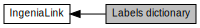
\includegraphics[width=272pt]{group__IL__DICT__LABELS}
\end{center}
\end{figure}
\subsection*{Typedefs}
\begin{DoxyCompactItemize}
\item 
typedef struct il\+\_\+dict\+\_\+labels \hyperlink{group__IL__DICT__LABELS_ga69d1109256f465cbcfa8aac7fa592495}{il\+\_\+dict\+\_\+labels\+\_\+t}
\begin{DoxyCompactList}\small\item\em Labels dictionary. \end{DoxyCompactList}\end{DoxyCompactItemize}
\subsection*{Functions}
\begin{DoxyCompactItemize}
\item 
\hyperlink{common_8h_a6bb629d26c52bfe10519ba3176853f47}{I\+L\+\_\+\+E\+X\+P\+O\+RT} \hyperlink{group__IL__DICT__LABELS_ga69d1109256f465cbcfa8aac7fa592495}{il\+\_\+dict\+\_\+labels\+\_\+t} $\ast$ \hyperlink{group__IL__DICT__LABELS_ga3d1801f1328932552ae98c151079514b}{il\+\_\+dict\+\_\+labels\+\_\+create} (void)
\begin{DoxyCompactList}\small\item\em Create a labels dictionary. \end{DoxyCompactList}\item 
\hyperlink{common_8h_a6bb629d26c52bfe10519ba3176853f47}{I\+L\+\_\+\+E\+X\+P\+O\+RT} void \hyperlink{group__IL__DICT__LABELS_ga5dbfa1bafc6fd6e5c1e3356579e6b03a}{il\+\_\+dict\+\_\+labels\+\_\+destroy} (\hyperlink{group__IL__DICT__LABELS_ga69d1109256f465cbcfa8aac7fa592495}{il\+\_\+dict\+\_\+labels\+\_\+t} $\ast$labels)
\begin{DoxyCompactList}\small\item\em Destroy a labels dictionary. \end{DoxyCompactList}\item 
\hyperlink{common_8h_a6bb629d26c52bfe10519ba3176853f47}{I\+L\+\_\+\+E\+X\+P\+O\+RT} int \hyperlink{group__IL__DICT__LABELS_ga40033ee8b33c612a90feec8ecfeaec40}{il\+\_\+dict\+\_\+labels\+\_\+get} (\hyperlink{group__IL__DICT__LABELS_ga69d1109256f465cbcfa8aac7fa592495}{il\+\_\+dict\+\_\+labels\+\_\+t} $\ast$labels, const char $\ast$lang, const char $\ast$$\ast$label)
\begin{DoxyCompactList}\small\item\em Obtain the label given a language. \end{DoxyCompactList}\item 
\hyperlink{common_8h_a6bb629d26c52bfe10519ba3176853f47}{I\+L\+\_\+\+E\+X\+P\+O\+RT} void \hyperlink{group__IL__DICT__LABELS_ga31c468b558ffe84fbd413883ce80eb84}{il\+\_\+dict\+\_\+labels\+\_\+set} (\hyperlink{group__IL__DICT__LABELS_ga69d1109256f465cbcfa8aac7fa592495}{il\+\_\+dict\+\_\+labels\+\_\+t} $\ast$labels, const char $\ast$lang, const char $\ast$label)
\begin{DoxyCompactList}\small\item\em Set the label for a given language. \end{DoxyCompactList}\item 
\hyperlink{common_8h_a6bb629d26c52bfe10519ba3176853f47}{I\+L\+\_\+\+E\+X\+P\+O\+RT} void \hyperlink{group__IL__DICT__LABELS_ga8910c8ced7a73f8971264ae83208c07e}{il\+\_\+dict\+\_\+labels\+\_\+del} (\hyperlink{group__IL__DICT__LABELS_ga69d1109256f465cbcfa8aac7fa592495}{il\+\_\+dict\+\_\+labels\+\_\+t} $\ast$labels, const char $\ast$lang)
\begin{DoxyCompactList}\small\item\em Remove the label of the given language. \end{DoxyCompactList}\item 
\hyperlink{common_8h_a6bb629d26c52bfe10519ba3176853f47}{I\+L\+\_\+\+E\+X\+P\+O\+RT} size\+\_\+t \hyperlink{group__IL__DICT__LABELS_gae088f90ebbe304009129f502da289122}{il\+\_\+dict\+\_\+labels\+\_\+nlabels\+\_\+get} (\hyperlink{group__IL__DICT__LABELS_ga69d1109256f465cbcfa8aac7fa592495}{il\+\_\+dict\+\_\+labels\+\_\+t} $\ast$labels)
\begin{DoxyCompactList}\small\item\em Obtain the number of labels. \end{DoxyCompactList}\item 
\hyperlink{common_8h_a6bb629d26c52bfe10519ba3176853f47}{I\+L\+\_\+\+E\+X\+P\+O\+RT} const char $\ast$$\ast$ \hyperlink{group__IL__DICT__LABELS_ga8fe3b029fc05420611468de19d2b6439}{il\+\_\+dict\+\_\+labels\+\_\+langs\+\_\+get} (\hyperlink{group__IL__DICT__LABELS_ga69d1109256f465cbcfa8aac7fa592495}{il\+\_\+dict\+\_\+labels\+\_\+t} $\ast$labels)
\begin{DoxyCompactList}\small\item\em Obtain the languages available in the labels dictionary. \end{DoxyCompactList}\item 
\hyperlink{common_8h_a6bb629d26c52bfe10519ba3176853f47}{I\+L\+\_\+\+E\+X\+P\+O\+RT} void \hyperlink{group__IL__DICT__LABELS_ga522d5f9739e165588a79e085d9112f06}{il\+\_\+dict\+\_\+labels\+\_\+langs\+\_\+destroy} (const char $\ast$$\ast$langs)
\begin{DoxyCompactList}\small\item\em Destroy a list of languages. \end{DoxyCompactList}\end{DoxyCompactItemize}


\subsection{Detailed Description}


\subsection{Typedef Documentation}
\index{Labels dictionary@{Labels dictionary}!il\+\_\+dict\+\_\+labels\+\_\+t@{il\+\_\+dict\+\_\+labels\+\_\+t}}
\index{il\+\_\+dict\+\_\+labels\+\_\+t@{il\+\_\+dict\+\_\+labels\+\_\+t}!Labels dictionary@{Labels dictionary}}
\subsubsection[{\texorpdfstring{il\+\_\+dict\+\_\+labels\+\_\+t}{il_dict_labels_t}}]{\setlength{\rightskip}{0pt plus 5cm}typedef struct il\+\_\+dict\+\_\+labels {\bf il\+\_\+dict\+\_\+labels\+\_\+t}}\hypertarget{group__IL__DICT__LABELS_ga69d1109256f465cbcfa8aac7fa592495}{}\label{group__IL__DICT__LABELS_ga69d1109256f465cbcfa8aac7fa592495}


Labels dictionary. 



\subsection{Function Documentation}
\index{Labels dictionary@{Labels dictionary}!il\+\_\+dict\+\_\+labels\+\_\+create@{il\+\_\+dict\+\_\+labels\+\_\+create}}
\index{il\+\_\+dict\+\_\+labels\+\_\+create@{il\+\_\+dict\+\_\+labels\+\_\+create}!Labels dictionary@{Labels dictionary}}
\subsubsection[{\texorpdfstring{il\+\_\+dict\+\_\+labels\+\_\+create(void)}{il_dict_labels_create(void)}}]{\setlength{\rightskip}{0pt plus 5cm}{\bf I\+L\+\_\+\+E\+X\+P\+O\+RT} {\bf il\+\_\+dict\+\_\+labels\+\_\+t}$\ast$ il\+\_\+dict\+\_\+labels\+\_\+create (
\begin{DoxyParamCaption}
\item[{void}]{}
\end{DoxyParamCaption}
)}\hypertarget{group__IL__DICT__LABELS_ga3d1801f1328932552ae98c151079514b}{}\label{group__IL__DICT__LABELS_ga3d1801f1328932552ae98c151079514b}


Create a labels dictionary. 

\begin{DoxyReturn}{Returns}
Labels dictionary instance (N\+U\+LL if it could not be created). 
\end{DoxyReturn}
\index{Labels dictionary@{Labels dictionary}!il\+\_\+dict\+\_\+labels\+\_\+del@{il\+\_\+dict\+\_\+labels\+\_\+del}}
\index{il\+\_\+dict\+\_\+labels\+\_\+del@{il\+\_\+dict\+\_\+labels\+\_\+del}!Labels dictionary@{Labels dictionary}}
\subsubsection[{\texorpdfstring{il\+\_\+dict\+\_\+labels\+\_\+del(il\+\_\+dict\+\_\+labels\+\_\+t $\ast$labels, const char $\ast$lang)}{il_dict_labels_del(il_dict_labels_t *labels, const char *lang)}}]{\setlength{\rightskip}{0pt plus 5cm}{\bf I\+L\+\_\+\+E\+X\+P\+O\+RT} void il\+\_\+dict\+\_\+labels\+\_\+del (
\begin{DoxyParamCaption}
\item[{{\bf il\+\_\+dict\+\_\+labels\+\_\+t} $\ast$}]{labels, }
\item[{const char $\ast$}]{lang}
\end{DoxyParamCaption}
)}\hypertarget{group__IL__DICT__LABELS_ga8910c8ced7a73f8971264ae83208c07e}{}\label{group__IL__DICT__LABELS_ga8910c8ced7a73f8971264ae83208c07e}


Remove the label of the given language. 


\begin{DoxyParams}[1]{Parameters}
\mbox{\tt in}  & {\em labels} & Labels dictionary. \\
\hline
\mbox{\tt in}  & {\em lang} & Language (I\+SO code). \\
\hline
\end{DoxyParams}
\index{Labels dictionary@{Labels dictionary}!il\+\_\+dict\+\_\+labels\+\_\+destroy@{il\+\_\+dict\+\_\+labels\+\_\+destroy}}
\index{il\+\_\+dict\+\_\+labels\+\_\+destroy@{il\+\_\+dict\+\_\+labels\+\_\+destroy}!Labels dictionary@{Labels dictionary}}
\subsubsection[{\texorpdfstring{il\+\_\+dict\+\_\+labels\+\_\+destroy(il\+\_\+dict\+\_\+labels\+\_\+t $\ast$labels)}{il_dict_labels_destroy(il_dict_labels_t *labels)}}]{\setlength{\rightskip}{0pt plus 5cm}{\bf I\+L\+\_\+\+E\+X\+P\+O\+RT} void il\+\_\+dict\+\_\+labels\+\_\+destroy (
\begin{DoxyParamCaption}
\item[{{\bf il\+\_\+dict\+\_\+labels\+\_\+t} $\ast$}]{labels}
\end{DoxyParamCaption}
)}\hypertarget{group__IL__DICT__LABELS_ga5dbfa1bafc6fd6e5c1e3356579e6b03a}{}\label{group__IL__DICT__LABELS_ga5dbfa1bafc6fd6e5c1e3356579e6b03a}


Destroy a labels dictionary. 


\begin{DoxyParams}[1]{Parameters}
\mbox{\tt in}  & {\em labels} & Labels dictionary. \\
\hline
\end{DoxyParams}
\index{Labels dictionary@{Labels dictionary}!il\+\_\+dict\+\_\+labels\+\_\+get@{il\+\_\+dict\+\_\+labels\+\_\+get}}
\index{il\+\_\+dict\+\_\+labels\+\_\+get@{il\+\_\+dict\+\_\+labels\+\_\+get}!Labels dictionary@{Labels dictionary}}
\subsubsection[{\texorpdfstring{il\+\_\+dict\+\_\+labels\+\_\+get(il\+\_\+dict\+\_\+labels\+\_\+t $\ast$labels, const char $\ast$lang, const char $\ast$$\ast$label)}{il_dict_labels_get(il_dict_labels_t *labels, const char *lang, const char **label)}}]{\setlength{\rightskip}{0pt plus 5cm}{\bf I\+L\+\_\+\+E\+X\+P\+O\+RT} int il\+\_\+dict\+\_\+labels\+\_\+get (
\begin{DoxyParamCaption}
\item[{{\bf il\+\_\+dict\+\_\+labels\+\_\+t} $\ast$}]{labels, }
\item[{const char $\ast$}]{lang, }
\item[{const char $\ast$$\ast$}]{label}
\end{DoxyParamCaption}
)}\hypertarget{group__IL__DICT__LABELS_ga40033ee8b33c612a90feec8ecfeaec40}{}\label{group__IL__DICT__LABELS_ga40033ee8b33c612a90feec8ecfeaec40}


Obtain the label given a language. 


\begin{DoxyParams}[1]{Parameters}
\mbox{\tt in}  & {\em labels} & Labels dictionary. \\
\hline
\mbox{\tt in}  & {\em lang} & Language (I\+SO code). \\
\hline
\mbox{\tt out}  & {\em label} & Label.\\
\hline
\end{DoxyParams}
\begin{DoxyReturn}{Returns}
0 if label exists for the given language, I\+L\+\_\+\+E\+F\+A\+IL otherwise. 
\end{DoxyReturn}
\begin{Desc}
\item[Examples\+: ]\par
\hyperlink{dict_8c-example}{dict.\+c}.\end{Desc}
\index{Labels dictionary@{Labels dictionary}!il\+\_\+dict\+\_\+labels\+\_\+langs\+\_\+destroy@{il\+\_\+dict\+\_\+labels\+\_\+langs\+\_\+destroy}}
\index{il\+\_\+dict\+\_\+labels\+\_\+langs\+\_\+destroy@{il\+\_\+dict\+\_\+labels\+\_\+langs\+\_\+destroy}!Labels dictionary@{Labels dictionary}}
\subsubsection[{\texorpdfstring{il\+\_\+dict\+\_\+labels\+\_\+langs\+\_\+destroy(const char $\ast$$\ast$langs)}{il_dict_labels_langs_destroy(const char **langs)}}]{\setlength{\rightskip}{0pt plus 5cm}{\bf I\+L\+\_\+\+E\+X\+P\+O\+RT} void il\+\_\+dict\+\_\+labels\+\_\+langs\+\_\+destroy (
\begin{DoxyParamCaption}
\item[{const char $\ast$$\ast$}]{langs}
\end{DoxyParamCaption}
)}\hypertarget{group__IL__DICT__LABELS_ga522d5f9739e165588a79e085d9112f06}{}\label{group__IL__DICT__LABELS_ga522d5f9739e165588a79e085d9112f06}


Destroy a list of languages. 


\begin{DoxyParams}[1]{Parameters}
\mbox{\tt in}  & {\em langs} & List of languages. \\
\hline
\end{DoxyParams}
\begin{Desc}
\item[Examples\+: ]\par
\hyperlink{dict_8c-example}{dict.\+c}.\end{Desc}
\index{Labels dictionary@{Labels dictionary}!il\+\_\+dict\+\_\+labels\+\_\+langs\+\_\+get@{il\+\_\+dict\+\_\+labels\+\_\+langs\+\_\+get}}
\index{il\+\_\+dict\+\_\+labels\+\_\+langs\+\_\+get@{il\+\_\+dict\+\_\+labels\+\_\+langs\+\_\+get}!Labels dictionary@{Labels dictionary}}
\subsubsection[{\texorpdfstring{il\+\_\+dict\+\_\+labels\+\_\+langs\+\_\+get(il\+\_\+dict\+\_\+labels\+\_\+t $\ast$labels)}{il_dict_labels_langs_get(il_dict_labels_t *labels)}}]{\setlength{\rightskip}{0pt plus 5cm}{\bf I\+L\+\_\+\+E\+X\+P\+O\+RT} const char$\ast$$\ast$ il\+\_\+dict\+\_\+labels\+\_\+langs\+\_\+get (
\begin{DoxyParamCaption}
\item[{{\bf il\+\_\+dict\+\_\+labels\+\_\+t} $\ast$}]{labels}
\end{DoxyParamCaption}
)}\hypertarget{group__IL__DICT__LABELS_ga8fe3b029fc05420611468de19d2b6439}{}\label{group__IL__DICT__LABELS_ga8fe3b029fc05420611468de19d2b6439}


Obtain the languages available in the labels dictionary. 


\begin{DoxyParams}[1]{Parameters}
\mbox{\tt in}  & {\em labels} & Labels dictionary.\\
\hline
\end{DoxyParams}
\begin{DoxyReturn}{Returns}
Null-\/terminated list of languages.
\end{DoxyReturn}
\begin{DoxySeeAlso}{See also}
\hyperlink{group__IL__DICT__LABELS_ga522d5f9739e165588a79e085d9112f06}{il\+\_\+dict\+\_\+labels\+\_\+langs\+\_\+destroy} 
\end{DoxySeeAlso}
\begin{Desc}
\item[Examples\+: ]\par
\hyperlink{dict_8c-example}{dict.\+c}.\end{Desc}
\index{Labels dictionary@{Labels dictionary}!il\+\_\+dict\+\_\+labels\+\_\+nlabels\+\_\+get@{il\+\_\+dict\+\_\+labels\+\_\+nlabels\+\_\+get}}
\index{il\+\_\+dict\+\_\+labels\+\_\+nlabels\+\_\+get@{il\+\_\+dict\+\_\+labels\+\_\+nlabels\+\_\+get}!Labels dictionary@{Labels dictionary}}
\subsubsection[{\texorpdfstring{il\+\_\+dict\+\_\+labels\+\_\+nlabels\+\_\+get(il\+\_\+dict\+\_\+labels\+\_\+t $\ast$labels)}{il_dict_labels_nlabels_get(il_dict_labels_t *labels)}}]{\setlength{\rightskip}{0pt plus 5cm}{\bf I\+L\+\_\+\+E\+X\+P\+O\+RT} size\+\_\+t il\+\_\+dict\+\_\+labels\+\_\+nlabels\+\_\+get (
\begin{DoxyParamCaption}
\item[{{\bf il\+\_\+dict\+\_\+labels\+\_\+t} $\ast$}]{labels}
\end{DoxyParamCaption}
)}\hypertarget{group__IL__DICT__LABELS_gae088f90ebbe304009129f502da289122}{}\label{group__IL__DICT__LABELS_gae088f90ebbe304009129f502da289122}


Obtain the number of labels. 


\begin{DoxyParams}[1]{Parameters}
\mbox{\tt in}  & {\em labels} & Labels dictionary. \\
\hline
\end{DoxyParams}
\begin{Desc}
\item[Examples\+: ]\par
\hyperlink{dict_8c-example}{dict.\+c}.\end{Desc}
\index{Labels dictionary@{Labels dictionary}!il\+\_\+dict\+\_\+labels\+\_\+set@{il\+\_\+dict\+\_\+labels\+\_\+set}}
\index{il\+\_\+dict\+\_\+labels\+\_\+set@{il\+\_\+dict\+\_\+labels\+\_\+set}!Labels dictionary@{Labels dictionary}}
\subsubsection[{\texorpdfstring{il\+\_\+dict\+\_\+labels\+\_\+set(il\+\_\+dict\+\_\+labels\+\_\+t $\ast$labels, const char $\ast$lang, const char $\ast$label)}{il_dict_labels_set(il_dict_labels_t *labels, const char *lang, const char *label)}}]{\setlength{\rightskip}{0pt plus 5cm}{\bf I\+L\+\_\+\+E\+X\+P\+O\+RT} void il\+\_\+dict\+\_\+labels\+\_\+set (
\begin{DoxyParamCaption}
\item[{{\bf il\+\_\+dict\+\_\+labels\+\_\+t} $\ast$}]{labels, }
\item[{const char $\ast$}]{lang, }
\item[{const char $\ast$}]{label}
\end{DoxyParamCaption}
)}\hypertarget{group__IL__DICT__LABELS_ga31c468b558ffe84fbd413883ce80eb84}{}\label{group__IL__DICT__LABELS_ga31c468b558ffe84fbd413883ce80eb84}


Set the label for a given language. 

\begin{DoxyNote}{Note}
A copy of label is stored internally.
\end{DoxyNote}

\begin{DoxyParams}[1]{Parameters}
\mbox{\tt in}  & {\em labels} & Labels dictionary. \\
\hline
\mbox{\tt in}  & {\em lang} & Language (I\+SO code). \\
\hline
\mbox{\tt in}  & {\em label} & Label. \\
\hline
\end{DoxyParams}

\hypertarget{group__IL__ERR}{}\section{Error reporting}
\label{group__IL__ERR}\index{Error reporting@{Error reporting}}
Collaboration diagram for Error reporting\+:\nopagebreak
\begin{figure}[H]
\begin{center}
\leavevmode
\includegraphics[width=260pt]{group__IL__ERR}
\end{center}
\end{figure}
\subsection*{Macros}
\begin{DoxyCompactItemize}
\item 
\#define \hyperlink{group__IL__ERR_ga19bb985b7d18cefc5aed42f9907fb2e0}{I\+L\+\_\+\+E\+F\+A\+IL}~-\/1
\begin{DoxyCompactList}\small\item\em General failure. \end{DoxyCompactList}\item 
\#define \hyperlink{group__IL__ERR_ga47cf82d575e6ab2f1af332b192f5a152}{I\+L\+\_\+\+E\+I\+N\+V\+AL}~-\/2
\begin{DoxyCompactList}\small\item\em Invalid values. \end{DoxyCompactList}\item 
\#define \hyperlink{group__IL__ERR_gac51a50be89cb8812586de3d7c403a3d2}{I\+L\+\_\+\+E\+T\+I\+M\+E\+D\+O\+UT}~-\/3
\begin{DoxyCompactList}\small\item\em Operation timed out. \end{DoxyCompactList}\item 
\#define \hyperlink{group__IL__ERR_gaf70f61bc8e6136b385edb92f72b0e676}{I\+L\+\_\+\+E\+N\+O\+M\+EM}~-\/4
\begin{DoxyCompactList}\small\item\em Not enough memory. \end{DoxyCompactList}\item 
\#define \hyperlink{group__IL__ERR_ga6450573c3dc43ce215afa857082692eb}{I\+L\+\_\+\+E\+A\+L\+R\+E\+A\+DY}~-\/5
\begin{DoxyCompactList}\small\item\em Already initialized. \end{DoxyCompactList}\item 
\#define \hyperlink{group__IL__ERR_ga09294945616872dde2c5ed98e257406d}{I\+L\+\_\+\+E\+D\+I\+S\+C\+O\+NN}~-\/6
\begin{DoxyCompactList}\small\item\em Device disconnected. \end{DoxyCompactList}\item 
\#define \hyperlink{group__IL__ERR_gaf8957a58cdc74c6cda94eb5bb990a26b}{I\+L\+\_\+\+E\+A\+C\+C\+E\+SS}~-\/7
\begin{DoxyCompactList}\small\item\em Access error. \end{DoxyCompactList}\item 
\#define \hyperlink{group__IL__ERR_ga85eb5ca72fd69575a0d927efcdd44188}{I\+L\+\_\+\+E\+S\+T\+A\+TE}~-\/8
\begin{DoxyCompactList}\small\item\em State error. \end{DoxyCompactList}\item 
\#define \hyperlink{group__IL__ERR_ga150b9efcf3d35150433b151f1f134b98}{I\+L\+\_\+\+E\+IO}~-\/9
\begin{DoxyCompactList}\small\item\em I/O error. \end{DoxyCompactList}\item 
\#define \hyperlink{group__IL__ERR_gacafae18e9ab826ace3f9135d2ed7deeb}{I\+L\+\_\+\+E\+N\+O\+T\+S\+UP}~-\/10
\begin{DoxyCompactList}\small\item\em Not supported. \end{DoxyCompactList}\end{DoxyCompactItemize}
\subsection*{Functions}
\begin{DoxyCompactItemize}
\item 
\hyperlink{common_8h_a6bb629d26c52bfe10519ba3176853f47}{I\+L\+\_\+\+E\+X\+P\+O\+RT} const char $\ast$ \hyperlink{group__IL__ERR_gac427087bdfe4aae17ff3e74de51cfe87}{ilerr\+\_\+last} (void)
\begin{DoxyCompactList}\small\item\em Obtain library last error details. \end{DoxyCompactList}\end{DoxyCompactItemize}


\subsection{Detailed Description}


\subsection{Macro Definition Documentation}
\index{Error reporting@{Error reporting}!I\+L\+\_\+\+E\+A\+C\+C\+E\+SS@{I\+L\+\_\+\+E\+A\+C\+C\+E\+SS}}
\index{I\+L\+\_\+\+E\+A\+C\+C\+E\+SS@{I\+L\+\_\+\+E\+A\+C\+C\+E\+SS}!Error reporting@{Error reporting}}
\subsubsection[{\texorpdfstring{I\+L\+\_\+\+E\+A\+C\+C\+E\+SS}{IL_EACCESS}}]{\setlength{\rightskip}{0pt plus 5cm}\#define I\+L\+\_\+\+E\+A\+C\+C\+E\+SS~-\/7}\hypertarget{group__IL__ERR_gaf8957a58cdc74c6cda94eb5bb990a26b}{}\label{group__IL__ERR_gaf8957a58cdc74c6cda94eb5bb990a26b}


Access error. 

\index{Error reporting@{Error reporting}!I\+L\+\_\+\+E\+A\+L\+R\+E\+A\+DY@{I\+L\+\_\+\+E\+A\+L\+R\+E\+A\+DY}}
\index{I\+L\+\_\+\+E\+A\+L\+R\+E\+A\+DY@{I\+L\+\_\+\+E\+A\+L\+R\+E\+A\+DY}!Error reporting@{Error reporting}}
\subsubsection[{\texorpdfstring{I\+L\+\_\+\+E\+A\+L\+R\+E\+A\+DY}{IL_EALREADY}}]{\setlength{\rightskip}{0pt plus 5cm}\#define I\+L\+\_\+\+E\+A\+L\+R\+E\+A\+DY~-\/5}\hypertarget{group__IL__ERR_ga6450573c3dc43ce215afa857082692eb}{}\label{group__IL__ERR_ga6450573c3dc43ce215afa857082692eb}


Already initialized. 

\index{Error reporting@{Error reporting}!I\+L\+\_\+\+E\+D\+I\+S\+C\+O\+NN@{I\+L\+\_\+\+E\+D\+I\+S\+C\+O\+NN}}
\index{I\+L\+\_\+\+E\+D\+I\+S\+C\+O\+NN@{I\+L\+\_\+\+E\+D\+I\+S\+C\+O\+NN}!Error reporting@{Error reporting}}
\subsubsection[{\texorpdfstring{I\+L\+\_\+\+E\+D\+I\+S\+C\+O\+NN}{IL_EDISCONN}}]{\setlength{\rightskip}{0pt plus 5cm}\#define I\+L\+\_\+\+E\+D\+I\+S\+C\+O\+NN~-\/6}\hypertarget{group__IL__ERR_ga09294945616872dde2c5ed98e257406d}{}\label{group__IL__ERR_ga09294945616872dde2c5ed98e257406d}


Device disconnected. 

\index{Error reporting@{Error reporting}!I\+L\+\_\+\+E\+F\+A\+IL@{I\+L\+\_\+\+E\+F\+A\+IL}}
\index{I\+L\+\_\+\+E\+F\+A\+IL@{I\+L\+\_\+\+E\+F\+A\+IL}!Error reporting@{Error reporting}}
\subsubsection[{\texorpdfstring{I\+L\+\_\+\+E\+F\+A\+IL}{IL_EFAIL}}]{\setlength{\rightskip}{0pt plus 5cm}\#define I\+L\+\_\+\+E\+F\+A\+IL~-\/1}\hypertarget{group__IL__ERR_ga19bb985b7d18cefc5aed42f9907fb2e0}{}\label{group__IL__ERR_ga19bb985b7d18cefc5aed42f9907fb2e0}


General failure. 

\index{Error reporting@{Error reporting}!I\+L\+\_\+\+E\+I\+N\+V\+AL@{I\+L\+\_\+\+E\+I\+N\+V\+AL}}
\index{I\+L\+\_\+\+E\+I\+N\+V\+AL@{I\+L\+\_\+\+E\+I\+N\+V\+AL}!Error reporting@{Error reporting}}
\subsubsection[{\texorpdfstring{I\+L\+\_\+\+E\+I\+N\+V\+AL}{IL_EINVAL}}]{\setlength{\rightskip}{0pt plus 5cm}\#define I\+L\+\_\+\+E\+I\+N\+V\+AL~-\/2}\hypertarget{group__IL__ERR_ga47cf82d575e6ab2f1af332b192f5a152}{}\label{group__IL__ERR_ga47cf82d575e6ab2f1af332b192f5a152}


Invalid values. 

\index{Error reporting@{Error reporting}!I\+L\+\_\+\+E\+IO@{I\+L\+\_\+\+E\+IO}}
\index{I\+L\+\_\+\+E\+IO@{I\+L\+\_\+\+E\+IO}!Error reporting@{Error reporting}}
\subsubsection[{\texorpdfstring{I\+L\+\_\+\+E\+IO}{IL_EIO}}]{\setlength{\rightskip}{0pt plus 5cm}\#define I\+L\+\_\+\+E\+IO~-\/9}\hypertarget{group__IL__ERR_ga150b9efcf3d35150433b151f1f134b98}{}\label{group__IL__ERR_ga150b9efcf3d35150433b151f1f134b98}


I/O error. 

\index{Error reporting@{Error reporting}!I\+L\+\_\+\+E\+N\+O\+M\+EM@{I\+L\+\_\+\+E\+N\+O\+M\+EM}}
\index{I\+L\+\_\+\+E\+N\+O\+M\+EM@{I\+L\+\_\+\+E\+N\+O\+M\+EM}!Error reporting@{Error reporting}}
\subsubsection[{\texorpdfstring{I\+L\+\_\+\+E\+N\+O\+M\+EM}{IL_ENOMEM}}]{\setlength{\rightskip}{0pt plus 5cm}\#define I\+L\+\_\+\+E\+N\+O\+M\+EM~-\/4}\hypertarget{group__IL__ERR_gaf70f61bc8e6136b385edb92f72b0e676}{}\label{group__IL__ERR_gaf70f61bc8e6136b385edb92f72b0e676}


Not enough memory. 

\index{Error reporting@{Error reporting}!I\+L\+\_\+\+E\+N\+O\+T\+S\+UP@{I\+L\+\_\+\+E\+N\+O\+T\+S\+UP}}
\index{I\+L\+\_\+\+E\+N\+O\+T\+S\+UP@{I\+L\+\_\+\+E\+N\+O\+T\+S\+UP}!Error reporting@{Error reporting}}
\subsubsection[{\texorpdfstring{I\+L\+\_\+\+E\+N\+O\+T\+S\+UP}{IL_ENOTSUP}}]{\setlength{\rightskip}{0pt plus 5cm}\#define I\+L\+\_\+\+E\+N\+O\+T\+S\+UP~-\/10}\hypertarget{group__IL__ERR_gacafae18e9ab826ace3f9135d2ed7deeb}{}\label{group__IL__ERR_gacafae18e9ab826ace3f9135d2ed7deeb}


Not supported. 

\index{Error reporting@{Error reporting}!I\+L\+\_\+\+E\+S\+T\+A\+TE@{I\+L\+\_\+\+E\+S\+T\+A\+TE}}
\index{I\+L\+\_\+\+E\+S\+T\+A\+TE@{I\+L\+\_\+\+E\+S\+T\+A\+TE}!Error reporting@{Error reporting}}
\subsubsection[{\texorpdfstring{I\+L\+\_\+\+E\+S\+T\+A\+TE}{IL_ESTATE}}]{\setlength{\rightskip}{0pt plus 5cm}\#define I\+L\+\_\+\+E\+S\+T\+A\+TE~-\/8}\hypertarget{group__IL__ERR_ga85eb5ca72fd69575a0d927efcdd44188}{}\label{group__IL__ERR_ga85eb5ca72fd69575a0d927efcdd44188}


State error. 

\index{Error reporting@{Error reporting}!I\+L\+\_\+\+E\+T\+I\+M\+E\+D\+O\+UT@{I\+L\+\_\+\+E\+T\+I\+M\+E\+D\+O\+UT}}
\index{I\+L\+\_\+\+E\+T\+I\+M\+E\+D\+O\+UT@{I\+L\+\_\+\+E\+T\+I\+M\+E\+D\+O\+UT}!Error reporting@{Error reporting}}
\subsubsection[{\texorpdfstring{I\+L\+\_\+\+E\+T\+I\+M\+E\+D\+O\+UT}{IL_ETIMEDOUT}}]{\setlength{\rightskip}{0pt plus 5cm}\#define I\+L\+\_\+\+E\+T\+I\+M\+E\+D\+O\+UT~-\/3}\hypertarget{group__IL__ERR_gac51a50be89cb8812586de3d7c403a3d2}{}\label{group__IL__ERR_gac51a50be89cb8812586de3d7c403a3d2}


Operation timed out. 



\subsection{Function Documentation}
\index{Error reporting@{Error reporting}!ilerr\+\_\+last@{ilerr\+\_\+last}}
\index{ilerr\+\_\+last@{ilerr\+\_\+last}!Error reporting@{Error reporting}}
\subsubsection[{\texorpdfstring{ilerr\+\_\+last(void)}{ilerr_last(void)}}]{\setlength{\rightskip}{0pt plus 5cm}{\bf I\+L\+\_\+\+E\+X\+P\+O\+RT} const char$\ast$ ilerr\+\_\+last (
\begin{DoxyParamCaption}
\item[{void}]{}
\end{DoxyParamCaption}
)}\hypertarget{group__IL__ERR_gac427087bdfe4aae17ff3e74de51cfe87}{}\label{group__IL__ERR_gac427087bdfe4aae17ff3e74de51cfe87}


Obtain library last error details. 

\begin{DoxyNote}{Note}
If host target supports thread local storage (T\+LS) the last error description is kept on a per-\/thread basis.
\end{DoxyNote}
\begin{DoxyReturn}{Returns}
Last error details. 
\end{DoxyReturn}
\begin{Desc}
\item[Examples\+: ]\par
\hyperlink{benchmark_8c-example}{benchmark.\+c}, \hyperlink{dict_8c-example}{dict.\+c}, \hyperlink{monitor_8c-example}{monitor.\+c}, \hyperlink{motion_8c-example}{motion.\+c}, and \hyperlink{servo_monitor_8c-example}{servo\+\_\+monitor.\+c}.\end{Desc}

\hypertarget{group__IL}{}\section{Ingenia\+Link}
\label{group__IL}\index{Ingenia\+Link@{Ingenia\+Link}}
Collaboration diagram for Ingenia\+Link\+:\nopagebreak
\begin{figure}[H]
\begin{center}
\leavevmode
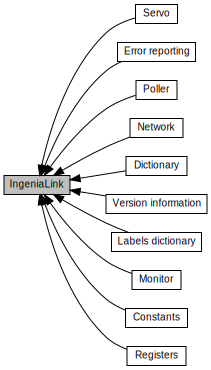
\includegraphics[width=283pt]{group__IL}
\end{center}
\end{figure}
\subsection*{Modules}
\begin{DoxyCompactItemize}
\item 
\hyperlink{group__IL__CONST}{Constants}
\item 
\hyperlink{group__IL__DICT}{Dictionary}
\item 
\hyperlink{group__IL__DICT__LABELS}{Labels dictionary}
\item 
\hyperlink{group__IL__ERR}{Error reporting}
\item 
\hyperlink{group__IL__MONITOR}{Monitor}
\item 
\hyperlink{group__IL__NET}{Network}
\item 
\hyperlink{group__IL__POLLER}{Poller}
\item 
\hyperlink{group__IL__REGS}{Registers}
\item 
\hyperlink{group__IL__SERVO}{Servo}
\item 
\hyperlink{group__IL__VERSION}{Version information}
\end{DoxyCompactItemize}
\subsection*{Files}
\begin{DoxyCompactItemize}
\item 
file \hyperlink{common_8h}{common.\+h}
\begin{DoxyCompactList}\small\item\em Common. \end{DoxyCompactList}\end{DoxyCompactItemize}


\subsection{Detailed Description}

\hypertarget{group__IL__MONITOR}{}\section{Monitor}
\label{group__IL__MONITOR}\index{Monitor@{Monitor}}
Collaboration diagram for Monitor\+:\nopagebreak
\begin{figure}[H]
\begin{center}
\leavevmode
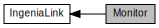
\includegraphics[width=231pt]{group__IL__MONITOR}
\end{center}
\end{figure}
\subsection*{Data Structures}
\begin{DoxyCompactItemize}
\item 
struct \hyperlink{structil__monitor__acq__t}{il\+\_\+monitor\+\_\+acq\+\_\+t}
\begin{DoxyCompactList}\small\item\em Monitor acquisition results. \end{DoxyCompactList}\end{DoxyCompactItemize}
\subsection*{Macros}
\begin{DoxyCompactItemize}
\item 
\#define \hyperlink{group__IL__MONITOR_ga05007f227fb5f253ed8ba714c0efb2cd}{I\+L\+\_\+\+M\+O\+N\+I\+T\+O\+R\+\_\+\+C\+H\+\_\+\+N\+UM}~4
\begin{DoxyCompactList}\small\item\em Number of channels. \end{DoxyCompactList}\end{DoxyCompactItemize}
\subsection*{Typedefs}
\begin{DoxyCompactItemize}
\item 
typedef struct il\+\_\+monitor \hyperlink{group__IL__MONITOR_ga40e12e851c8c83202f0bccbaaafbc1f3}{il\+\_\+monitor\+\_\+t}
\begin{DoxyCompactList}\small\item\em Ingenia\+Link monitor. \end{DoxyCompactList}\end{DoxyCompactItemize}
\subsection*{Enumerations}
\begin{DoxyCompactItemize}
\item 
enum \hyperlink{group__IL__MONITOR_ga713d0c15082ee67cb77d384d4537e107}{il\+\_\+monitor\+\_\+trigger\+\_\+t} \{ \\*
\hyperlink{group__IL__MONITOR_gga713d0c15082ee67cb77d384d4537e107a7a2adbfffa9d5301d44c58aee1524947}{I\+L\+\_\+\+M\+O\+N\+I\+T\+O\+R\+\_\+\+T\+R\+I\+G\+G\+E\+R\+\_\+\+I\+M\+M\+E\+D\+I\+A\+TE} = 0, 
\hyperlink{group__IL__MONITOR_gga713d0c15082ee67cb77d384d4537e107a3d9776dc06a1769bb3bac474d0d2f671}{I\+L\+\_\+\+M\+O\+N\+I\+T\+O\+R\+\_\+\+T\+R\+I\+G\+G\+E\+R\+\_\+\+M\+O\+T\+I\+ON} = 1, 
\hyperlink{group__IL__MONITOR_gga713d0c15082ee67cb77d384d4537e107a3e127c86c21f607d0df72b64403adb42}{I\+L\+\_\+\+M\+O\+N\+I\+T\+O\+R\+\_\+\+T\+R\+I\+G\+G\+E\+R\+\_\+\+P\+OS} = 2, 
\hyperlink{group__IL__MONITOR_gga713d0c15082ee67cb77d384d4537e107afff4584d639834baa2242e2ab08aafd6}{I\+L\+\_\+\+M\+O\+N\+I\+T\+O\+R\+\_\+\+T\+R\+I\+G\+G\+E\+R\+\_\+\+N\+EG} = 3, 
\\*
\hyperlink{group__IL__MONITOR_gga713d0c15082ee67cb77d384d4537e107af66901be0c630d815042a98f13b0781b}{I\+L\+\_\+\+M\+O\+N\+I\+T\+O\+R\+\_\+\+T\+R\+I\+G\+G\+E\+R\+\_\+\+W\+I\+N\+D\+OW} = 4, 
\hyperlink{group__IL__MONITOR_gga713d0c15082ee67cb77d384d4537e107aededed6d0aa1e43dd19b0019f857db06}{I\+L\+\_\+\+M\+O\+N\+I\+T\+O\+R\+\_\+\+T\+R\+I\+G\+G\+E\+R\+\_\+\+D\+IN} = 5
 \}\begin{DoxyCompactList}\small\item\em Trigger modes. \end{DoxyCompactList}
\end{DoxyCompactItemize}
\subsection*{Functions}
\begin{DoxyCompactItemize}
\item 
\hyperlink{common_8h_a6bb629d26c52bfe10519ba3176853f47}{I\+L\+\_\+\+E\+X\+P\+O\+RT} \hyperlink{group__IL__MONITOR_ga40e12e851c8c83202f0bccbaaafbc1f3}{il\+\_\+monitor\+\_\+t} $\ast$ \hyperlink{group__IL__MONITOR_gabab1b2d47a46eeabfcaa9ec5ce7c49a8}{il\+\_\+monitor\+\_\+create} (\hyperlink{group__IL__SERVO_ga3369ddfcc33492fe3a28f96cf455b13e}{il\+\_\+servo\+\_\+t} $\ast$servo)
\begin{DoxyCompactList}\small\item\em Create monitor instance. \end{DoxyCompactList}\item 
\hyperlink{common_8h_a6bb629d26c52bfe10519ba3176853f47}{I\+L\+\_\+\+E\+X\+P\+O\+RT} void \hyperlink{group__IL__MONITOR_ga3bc1e187d696eadd07a3f33b502c998a}{il\+\_\+monitor\+\_\+destroy} (\hyperlink{group__IL__MONITOR_ga40e12e851c8c83202f0bccbaaafbc1f3}{il\+\_\+monitor\+\_\+t} $\ast$monitor)
\begin{DoxyCompactList}\small\item\em Destroy a monitor instance. \end{DoxyCompactList}\item 
\hyperlink{common_8h_a6bb629d26c52bfe10519ba3176853f47}{I\+L\+\_\+\+E\+X\+P\+O\+RT} int \hyperlink{group__IL__MONITOR_ga41ec8c974f4322537d714844be7b8a2a}{il\+\_\+monitor\+\_\+start} (\hyperlink{group__IL__MONITOR_ga40e12e851c8c83202f0bccbaaafbc1f3}{il\+\_\+monitor\+\_\+t} $\ast$monitor)
\begin{DoxyCompactList}\small\item\em Start monitor. \end{DoxyCompactList}\item 
\hyperlink{common_8h_a6bb629d26c52bfe10519ba3176853f47}{I\+L\+\_\+\+E\+X\+P\+O\+RT} void \hyperlink{group__IL__MONITOR_ga2408490312f9562407f93111a4deece8}{il\+\_\+monitor\+\_\+stop} (\hyperlink{group__IL__MONITOR_ga40e12e851c8c83202f0bccbaaafbc1f3}{il\+\_\+monitor\+\_\+t} $\ast$monitor)
\begin{DoxyCompactList}\small\item\em Stop monitor. \end{DoxyCompactList}\item 
\hyperlink{common_8h_a6bb629d26c52bfe10519ba3176853f47}{I\+L\+\_\+\+E\+X\+P\+O\+RT} int \hyperlink{group__IL__MONITOR_ga5a2bfd4b0f37f4abee986a77afae5b32}{il\+\_\+monitor\+\_\+wait} (\hyperlink{group__IL__MONITOR_ga40e12e851c8c83202f0bccbaaafbc1f3}{il\+\_\+monitor\+\_\+t} $\ast$monitor, int timeout)
\begin{DoxyCompactList}\small\item\em Wait until current acquisition is completed. \end{DoxyCompactList}\item 
\hyperlink{common_8h_a6bb629d26c52bfe10519ba3176853f47}{I\+L\+\_\+\+E\+X\+P\+O\+RT} void \hyperlink{group__IL__MONITOR_gad6231f5d154969361fdd05d3f84707bb}{il\+\_\+monitor\+\_\+data\+\_\+get} (\hyperlink{group__IL__MONITOR_ga40e12e851c8c83202f0bccbaaafbc1f3}{il\+\_\+monitor\+\_\+t} $\ast$monitor, \hyperlink{structil__monitor__acq__t}{il\+\_\+monitor\+\_\+acq\+\_\+t} $\ast$$\ast$acq)
\begin{DoxyCompactList}\small\item\em Obtain current available data. \end{DoxyCompactList}\item 
\hyperlink{common_8h_a6bb629d26c52bfe10519ba3176853f47}{I\+L\+\_\+\+E\+X\+P\+O\+RT} int \hyperlink{group__IL__MONITOR_ga8fc675f7d849ebcf162e396a98b6c710}{il\+\_\+monitor\+\_\+configure} (\hyperlink{group__IL__MONITOR_ga40e12e851c8c83202f0bccbaaafbc1f3}{il\+\_\+monitor\+\_\+t} $\ast$monitor, unsigned int t\+\_\+s, size\+\_\+t delay\+\_\+samples, size\+\_\+t max\+\_\+samples)
\begin{DoxyCompactList}\small\item\em Configure monitor parameters. \end{DoxyCompactList}\item 
\hyperlink{common_8h_a6bb629d26c52bfe10519ba3176853f47}{I\+L\+\_\+\+E\+X\+P\+O\+RT} int \hyperlink{group__IL__MONITOR_gacda4fa0bc57e96988e62f895b256a62a}{il\+\_\+monitor\+\_\+ch\+\_\+configure} (\hyperlink{group__IL__MONITOR_ga40e12e851c8c83202f0bccbaaafbc1f3}{il\+\_\+monitor\+\_\+t} $\ast$monitor, int ch, const \hyperlink{structil__reg__t}{il\+\_\+reg\+\_\+t} $\ast$reg, const char $\ast$id)
\begin{DoxyCompactList}\small\item\em Configure channel mapping. \end{DoxyCompactList}\item 
\hyperlink{common_8h_a6bb629d26c52bfe10519ba3176853f47}{I\+L\+\_\+\+E\+X\+P\+O\+RT} int \hyperlink{group__IL__MONITOR_ga33dffe1563b9d4a53d7623a123d7710c}{il\+\_\+monitor\+\_\+ch\+\_\+disable} (\hyperlink{group__IL__MONITOR_ga40e12e851c8c83202f0bccbaaafbc1f3}{il\+\_\+monitor\+\_\+t} $\ast$monitor, int ch)
\begin{DoxyCompactList}\small\item\em Disable one channel. \end{DoxyCompactList}\item 
\hyperlink{common_8h_a6bb629d26c52bfe10519ba3176853f47}{I\+L\+\_\+\+E\+X\+P\+O\+RT} int \hyperlink{group__IL__MONITOR_ga19230bb2f539a808deb9e42afcb58678}{il\+\_\+monitor\+\_\+ch\+\_\+disable\+\_\+all} (\hyperlink{group__IL__MONITOR_ga40e12e851c8c83202f0bccbaaafbc1f3}{il\+\_\+monitor\+\_\+t} $\ast$monitor)
\begin{DoxyCompactList}\small\item\em Disable all channels. \end{DoxyCompactList}\item 
\hyperlink{common_8h_a6bb629d26c52bfe10519ba3176853f47}{I\+L\+\_\+\+E\+X\+P\+O\+RT} int \hyperlink{group__IL__MONITOR_ga98522072a54d7e70fe94409d666d58cd}{il\+\_\+monitor\+\_\+trigger\+\_\+configure} (\hyperlink{group__IL__MONITOR_ga40e12e851c8c83202f0bccbaaafbc1f3}{il\+\_\+monitor\+\_\+t} $\ast$monitor, \hyperlink{group__IL__MONITOR_ga713d0c15082ee67cb77d384d4537e107}{il\+\_\+monitor\+\_\+trigger\+\_\+t} mode, size\+\_\+t delay\+\_\+samples, const \hyperlink{structil__reg__t}{il\+\_\+reg\+\_\+t} $\ast$source, const char $\ast$source\+\_\+id, double th\+\_\+pos, double th\+\_\+neg, uint32\+\_\+t din\+\_\+msk)
\begin{DoxyCompactList}\small\item\em Trigger configuration. \end{DoxyCompactList}\end{DoxyCompactItemize}


\subsection{Detailed Description}


\subsection{Macro Definition Documentation}
\index{Monitor@{Monitor}!I\+L\+\_\+\+M\+O\+N\+I\+T\+O\+R\+\_\+\+C\+H\+\_\+\+N\+UM@{I\+L\+\_\+\+M\+O\+N\+I\+T\+O\+R\+\_\+\+C\+H\+\_\+\+N\+UM}}
\index{I\+L\+\_\+\+M\+O\+N\+I\+T\+O\+R\+\_\+\+C\+H\+\_\+\+N\+UM@{I\+L\+\_\+\+M\+O\+N\+I\+T\+O\+R\+\_\+\+C\+H\+\_\+\+N\+UM}!Monitor@{Monitor}}
\subsubsection[{\texorpdfstring{I\+L\+\_\+\+M\+O\+N\+I\+T\+O\+R\+\_\+\+C\+H\+\_\+\+N\+UM}{IL_MONITOR_CH_NUM}}]{\setlength{\rightskip}{0pt plus 5cm}\#define I\+L\+\_\+\+M\+O\+N\+I\+T\+O\+R\+\_\+\+C\+H\+\_\+\+N\+UM~4}\hypertarget{group__IL__MONITOR_ga05007f227fb5f253ed8ba714c0efb2cd}{}\label{group__IL__MONITOR_ga05007f227fb5f253ed8ba714c0efb2cd}


Number of channels. 



\subsection{Typedef Documentation}
\index{Monitor@{Monitor}!il\+\_\+monitor\+\_\+t@{il\+\_\+monitor\+\_\+t}}
\index{il\+\_\+monitor\+\_\+t@{il\+\_\+monitor\+\_\+t}!Monitor@{Monitor}}
\subsubsection[{\texorpdfstring{il\+\_\+monitor\+\_\+t}{il_monitor_t}}]{\setlength{\rightskip}{0pt plus 5cm}typedef struct il\+\_\+monitor {\bf il\+\_\+monitor\+\_\+t}}\hypertarget{group__IL__MONITOR_ga40e12e851c8c83202f0bccbaaafbc1f3}{}\label{group__IL__MONITOR_ga40e12e851c8c83202f0bccbaaafbc1f3}


Ingenia\+Link monitor. 



\subsection{Enumeration Type Documentation}
\index{Monitor@{Monitor}!il\+\_\+monitor\+\_\+trigger\+\_\+t@{il\+\_\+monitor\+\_\+trigger\+\_\+t}}
\index{il\+\_\+monitor\+\_\+trigger\+\_\+t@{il\+\_\+monitor\+\_\+trigger\+\_\+t}!Monitor@{Monitor}}
\subsubsection[{\texorpdfstring{il\+\_\+monitor\+\_\+trigger\+\_\+t}{il_monitor_trigger_t}}]{\setlength{\rightskip}{0pt plus 5cm}enum {\bf il\+\_\+monitor\+\_\+trigger\+\_\+t}}\hypertarget{group__IL__MONITOR_ga713d0c15082ee67cb77d384d4537e107}{}\label{group__IL__MONITOR_ga713d0c15082ee67cb77d384d4537e107}


Trigger modes. 

\begin{Desc}
\item[Enumerator]\par
\begin{description}
\index{I\+L\+\_\+\+M\+O\+N\+I\+T\+O\+R\+\_\+\+T\+R\+I\+G\+G\+E\+R\+\_\+\+I\+M\+M\+E\+D\+I\+A\+TE@{I\+L\+\_\+\+M\+O\+N\+I\+T\+O\+R\+\_\+\+T\+R\+I\+G\+G\+E\+R\+\_\+\+I\+M\+M\+E\+D\+I\+A\+TE}!Monitor@{Monitor}}\index{Monitor@{Monitor}!I\+L\+\_\+\+M\+O\+N\+I\+T\+O\+R\+\_\+\+T\+R\+I\+G\+G\+E\+R\+\_\+\+I\+M\+M\+E\+D\+I\+A\+TE@{I\+L\+\_\+\+M\+O\+N\+I\+T\+O\+R\+\_\+\+T\+R\+I\+G\+G\+E\+R\+\_\+\+I\+M\+M\+E\+D\+I\+A\+TE}}\item[{\em 
I\+L\+\_\+\+M\+O\+N\+I\+T\+O\+R\+\_\+\+T\+R\+I\+G\+G\+E\+R\+\_\+\+I\+M\+M\+E\+D\+I\+A\+TE\hypertarget{group__IL__MONITOR_gga713d0c15082ee67cb77d384d4537e107a7a2adbfffa9d5301d44c58aee1524947}{}\label{group__IL__MONITOR_gga713d0c15082ee67cb77d384d4537e107a7a2adbfffa9d5301d44c58aee1524947}
}]Immediate. \index{I\+L\+\_\+\+M\+O\+N\+I\+T\+O\+R\+\_\+\+T\+R\+I\+G\+G\+E\+R\+\_\+\+M\+O\+T\+I\+ON@{I\+L\+\_\+\+M\+O\+N\+I\+T\+O\+R\+\_\+\+T\+R\+I\+G\+G\+E\+R\+\_\+\+M\+O\+T\+I\+ON}!Monitor@{Monitor}}\index{Monitor@{Monitor}!I\+L\+\_\+\+M\+O\+N\+I\+T\+O\+R\+\_\+\+T\+R\+I\+G\+G\+E\+R\+\_\+\+M\+O\+T\+I\+ON@{I\+L\+\_\+\+M\+O\+N\+I\+T\+O\+R\+\_\+\+T\+R\+I\+G\+G\+E\+R\+\_\+\+M\+O\+T\+I\+ON}}\item[{\em 
I\+L\+\_\+\+M\+O\+N\+I\+T\+O\+R\+\_\+\+T\+R\+I\+G\+G\+E\+R\+\_\+\+M\+O\+T\+I\+ON\hypertarget{group__IL__MONITOR_gga713d0c15082ee67cb77d384d4537e107a3d9776dc06a1769bb3bac474d0d2f671}{}\label{group__IL__MONITOR_gga713d0c15082ee67cb77d384d4537e107a3d9776dc06a1769bb3bac474d0d2f671}
}]Motion start. \index{I\+L\+\_\+\+M\+O\+N\+I\+T\+O\+R\+\_\+\+T\+R\+I\+G\+G\+E\+R\+\_\+\+P\+OS@{I\+L\+\_\+\+M\+O\+N\+I\+T\+O\+R\+\_\+\+T\+R\+I\+G\+G\+E\+R\+\_\+\+P\+OS}!Monitor@{Monitor}}\index{Monitor@{Monitor}!I\+L\+\_\+\+M\+O\+N\+I\+T\+O\+R\+\_\+\+T\+R\+I\+G\+G\+E\+R\+\_\+\+P\+OS@{I\+L\+\_\+\+M\+O\+N\+I\+T\+O\+R\+\_\+\+T\+R\+I\+G\+G\+E\+R\+\_\+\+P\+OS}}\item[{\em 
I\+L\+\_\+\+M\+O\+N\+I\+T\+O\+R\+\_\+\+T\+R\+I\+G\+G\+E\+R\+\_\+\+P\+OS\hypertarget{group__IL__MONITOR_gga713d0c15082ee67cb77d384d4537e107a3e127c86c21f607d0df72b64403adb42}{}\label{group__IL__MONITOR_gga713d0c15082ee67cb77d384d4537e107a3e127c86c21f607d0df72b64403adb42}
}]Positive slope. \index{I\+L\+\_\+\+M\+O\+N\+I\+T\+O\+R\+\_\+\+T\+R\+I\+G\+G\+E\+R\+\_\+\+N\+EG@{I\+L\+\_\+\+M\+O\+N\+I\+T\+O\+R\+\_\+\+T\+R\+I\+G\+G\+E\+R\+\_\+\+N\+EG}!Monitor@{Monitor}}\index{Monitor@{Monitor}!I\+L\+\_\+\+M\+O\+N\+I\+T\+O\+R\+\_\+\+T\+R\+I\+G\+G\+E\+R\+\_\+\+N\+EG@{I\+L\+\_\+\+M\+O\+N\+I\+T\+O\+R\+\_\+\+T\+R\+I\+G\+G\+E\+R\+\_\+\+N\+EG}}\item[{\em 
I\+L\+\_\+\+M\+O\+N\+I\+T\+O\+R\+\_\+\+T\+R\+I\+G\+G\+E\+R\+\_\+\+N\+EG\hypertarget{group__IL__MONITOR_gga713d0c15082ee67cb77d384d4537e107afff4584d639834baa2242e2ab08aafd6}{}\label{group__IL__MONITOR_gga713d0c15082ee67cb77d384d4537e107afff4584d639834baa2242e2ab08aafd6}
}]Negative slope. \index{I\+L\+\_\+\+M\+O\+N\+I\+T\+O\+R\+\_\+\+T\+R\+I\+G\+G\+E\+R\+\_\+\+W\+I\+N\+D\+OW@{I\+L\+\_\+\+M\+O\+N\+I\+T\+O\+R\+\_\+\+T\+R\+I\+G\+G\+E\+R\+\_\+\+W\+I\+N\+D\+OW}!Monitor@{Monitor}}\index{Monitor@{Monitor}!I\+L\+\_\+\+M\+O\+N\+I\+T\+O\+R\+\_\+\+T\+R\+I\+G\+G\+E\+R\+\_\+\+W\+I\+N\+D\+OW@{I\+L\+\_\+\+M\+O\+N\+I\+T\+O\+R\+\_\+\+T\+R\+I\+G\+G\+E\+R\+\_\+\+W\+I\+N\+D\+OW}}\item[{\em 
I\+L\+\_\+\+M\+O\+N\+I\+T\+O\+R\+\_\+\+T\+R\+I\+G\+G\+E\+R\+\_\+\+W\+I\+N\+D\+OW\hypertarget{group__IL__MONITOR_gga713d0c15082ee67cb77d384d4537e107af66901be0c630d815042a98f13b0781b}{}\label{group__IL__MONITOR_gga713d0c15082ee67cb77d384d4537e107af66901be0c630d815042a98f13b0781b}
}]Exit window. \index{I\+L\+\_\+\+M\+O\+N\+I\+T\+O\+R\+\_\+\+T\+R\+I\+G\+G\+E\+R\+\_\+\+D\+IN@{I\+L\+\_\+\+M\+O\+N\+I\+T\+O\+R\+\_\+\+T\+R\+I\+G\+G\+E\+R\+\_\+\+D\+IN}!Monitor@{Monitor}}\index{Monitor@{Monitor}!I\+L\+\_\+\+M\+O\+N\+I\+T\+O\+R\+\_\+\+T\+R\+I\+G\+G\+E\+R\+\_\+\+D\+IN@{I\+L\+\_\+\+M\+O\+N\+I\+T\+O\+R\+\_\+\+T\+R\+I\+G\+G\+E\+R\+\_\+\+D\+IN}}\item[{\em 
I\+L\+\_\+\+M\+O\+N\+I\+T\+O\+R\+\_\+\+T\+R\+I\+G\+G\+E\+R\+\_\+\+D\+IN\hypertarget{group__IL__MONITOR_gga713d0c15082ee67cb77d384d4537e107aededed6d0aa1e43dd19b0019f857db06}{}\label{group__IL__MONITOR_gga713d0c15082ee67cb77d384d4537e107aededed6d0aa1e43dd19b0019f857db06}
}]Digital input activation. \end{description}
\end{Desc}


\subsection{Function Documentation}
\index{Monitor@{Monitor}!il\+\_\+monitor\+\_\+ch\+\_\+configure@{il\+\_\+monitor\+\_\+ch\+\_\+configure}}
\index{il\+\_\+monitor\+\_\+ch\+\_\+configure@{il\+\_\+monitor\+\_\+ch\+\_\+configure}!Monitor@{Monitor}}
\subsubsection[{\texorpdfstring{il\+\_\+monitor\+\_\+ch\+\_\+configure(il\+\_\+monitor\+\_\+t $\ast$monitor, int ch, const il\+\_\+reg\+\_\+t $\ast$reg, const char $\ast$id)}{il_monitor_ch_configure(il_monitor_t *monitor, int ch, const il_reg_t *reg, const char *id)}}]{\setlength{\rightskip}{0pt plus 5cm}{\bf I\+L\+\_\+\+E\+X\+P\+O\+RT} int il\+\_\+monitor\+\_\+ch\+\_\+configure (
\begin{DoxyParamCaption}
\item[{{\bf il\+\_\+monitor\+\_\+t} $\ast$}]{monitor, }
\item[{int}]{ch, }
\item[{const {\bf il\+\_\+reg\+\_\+t} $\ast$}]{reg, }
\item[{const char $\ast$}]{id}
\end{DoxyParamCaption}
)}\hypertarget{group__IL__MONITOR_gacda4fa0bc57e96988e62f895b256a62a}{}\label{group__IL__MONITOR_gacda4fa0bc57e96988e62f895b256a62a}


Configure channel mapping. 


\begin{DoxyParams}[1]{Parameters}
\mbox{\tt in}  & {\em monitor} & Monitor instance. \\
\hline
\mbox{\tt in}  & {\em ch} & Channel to be configured (0-\/3). \\
\hline
\mbox{\tt in}  & {\em reg} & Register (pre-\/defined) to be mapped on the channel. \\
\hline
\mbox{\tt in}  & {\em id} & Register ID to be mapped on the channel.\\
\hline
\end{DoxyParams}
\begin{DoxyReturn}{Returns}
0 on success, error code otherwise. 
\end{DoxyReturn}
\begin{Desc}
\item[Examples\+: ]\par
\hyperlink{monitor_8c-example}{monitor.\+c}.\end{Desc}
\index{Monitor@{Monitor}!il\+\_\+monitor\+\_\+ch\+\_\+disable@{il\+\_\+monitor\+\_\+ch\+\_\+disable}}
\index{il\+\_\+monitor\+\_\+ch\+\_\+disable@{il\+\_\+monitor\+\_\+ch\+\_\+disable}!Monitor@{Monitor}}
\subsubsection[{\texorpdfstring{il\+\_\+monitor\+\_\+ch\+\_\+disable(il\+\_\+monitor\+\_\+t $\ast$monitor, int ch)}{il_monitor_ch_disable(il_monitor_t *monitor, int ch)}}]{\setlength{\rightskip}{0pt plus 5cm}{\bf I\+L\+\_\+\+E\+X\+P\+O\+RT} int il\+\_\+monitor\+\_\+ch\+\_\+disable (
\begin{DoxyParamCaption}
\item[{{\bf il\+\_\+monitor\+\_\+t} $\ast$}]{monitor, }
\item[{int}]{ch}
\end{DoxyParamCaption}
)}\hypertarget{group__IL__MONITOR_ga33dffe1563b9d4a53d7623a123d7710c}{}\label{group__IL__MONITOR_ga33dffe1563b9d4a53d7623a123d7710c}


Disable one channel. 


\begin{DoxyParams}[1]{Parameters}
\mbox{\tt in}  & {\em monitor} & Monitor instance. \\
\hline
\mbox{\tt in}  & {\em ch} & Channel to be disabled (0-\/3).\\
\hline
\end{DoxyParams}
\begin{DoxyReturn}{Returns}
0 on success, error code otherwise. 
\end{DoxyReturn}
\index{Monitor@{Monitor}!il\+\_\+monitor\+\_\+ch\+\_\+disable\+\_\+all@{il\+\_\+monitor\+\_\+ch\+\_\+disable\+\_\+all}}
\index{il\+\_\+monitor\+\_\+ch\+\_\+disable\+\_\+all@{il\+\_\+monitor\+\_\+ch\+\_\+disable\+\_\+all}!Monitor@{Monitor}}
\subsubsection[{\texorpdfstring{il\+\_\+monitor\+\_\+ch\+\_\+disable\+\_\+all(il\+\_\+monitor\+\_\+t $\ast$monitor)}{il_monitor_ch_disable_all(il_monitor_t *monitor)}}]{\setlength{\rightskip}{0pt plus 5cm}{\bf I\+L\+\_\+\+E\+X\+P\+O\+RT} int il\+\_\+monitor\+\_\+ch\+\_\+disable\+\_\+all (
\begin{DoxyParamCaption}
\item[{{\bf il\+\_\+monitor\+\_\+t} $\ast$}]{monitor}
\end{DoxyParamCaption}
)}\hypertarget{group__IL__MONITOR_ga19230bb2f539a808deb9e42afcb58678}{}\label{group__IL__MONITOR_ga19230bb2f539a808deb9e42afcb58678}


Disable all channels. 


\begin{DoxyParams}[1]{Parameters}
\mbox{\tt in}  & {\em monitor} & Monitor instance.\\
\hline
\end{DoxyParams}
\begin{DoxyReturn}{Returns}
0 on success, error code otherwise. 
\end{DoxyReturn}
\index{Monitor@{Monitor}!il\+\_\+monitor\+\_\+configure@{il\+\_\+monitor\+\_\+configure}}
\index{il\+\_\+monitor\+\_\+configure@{il\+\_\+monitor\+\_\+configure}!Monitor@{Monitor}}
\subsubsection[{\texorpdfstring{il\+\_\+monitor\+\_\+configure(il\+\_\+monitor\+\_\+t $\ast$monitor, unsigned int t\+\_\+s, size\+\_\+t delay\+\_\+samples, size\+\_\+t max\+\_\+samples)}{il_monitor_configure(il_monitor_t *monitor, unsigned int t_s, size_t delay_samples, size_t max_samples)}}]{\setlength{\rightskip}{0pt plus 5cm}{\bf I\+L\+\_\+\+E\+X\+P\+O\+RT} int il\+\_\+monitor\+\_\+configure (
\begin{DoxyParamCaption}
\item[{{\bf il\+\_\+monitor\+\_\+t} $\ast$}]{monitor, }
\item[{unsigned int}]{t\+\_\+s, }
\item[{size\+\_\+t}]{delay\+\_\+samples, }
\item[{size\+\_\+t}]{max\+\_\+samples}
\end{DoxyParamCaption}
)}\hypertarget{group__IL__MONITOR_ga8fc675f7d849ebcf162e396a98b6c710}{}\label{group__IL__MONITOR_ga8fc675f7d849ebcf162e396a98b6c710}


Configure monitor parameters. 

\begin{DoxyNote}{Note}

\begin{DoxyItemize}
\item The monitor maximum resolution is 100 us.
\item The monitor maximum number of samples depends on the configured mappings.
\end{DoxyItemize}
\end{DoxyNote}

\begin{DoxyParams}[1]{Parameters}
\mbox{\tt in}  & {\em monitor} & Monitor instance. \\
\hline
\mbox{\tt in}  & {\em t\+\_\+s} & Sampling period (us). \\
\hline
\mbox{\tt in}  & {\em delay\+\_\+samples} & Delay samples. \\
\hline
\mbox{\tt in}  & {\em max\+\_\+samples} & Maximum number of samples to acquire (use 0 to use the maximum).\\
\hline
\end{DoxyParams}
\begin{DoxyReturn}{Returns}
0 on success, error code otherwise. 
\end{DoxyReturn}
\begin{Desc}
\item[Examples\+: ]\par
\hyperlink{monitor_8c-example}{monitor.\+c}.\end{Desc}
\index{Monitor@{Monitor}!il\+\_\+monitor\+\_\+create@{il\+\_\+monitor\+\_\+create}}
\index{il\+\_\+monitor\+\_\+create@{il\+\_\+monitor\+\_\+create}!Monitor@{Monitor}}
\subsubsection[{\texorpdfstring{il\+\_\+monitor\+\_\+create(il\+\_\+servo\+\_\+t $\ast$servo)}{il_monitor_create(il_servo_t *servo)}}]{\setlength{\rightskip}{0pt plus 5cm}{\bf I\+L\+\_\+\+E\+X\+P\+O\+RT} {\bf il\+\_\+monitor\+\_\+t}$\ast$ il\+\_\+monitor\+\_\+create (
\begin{DoxyParamCaption}
\item[{{\bf il\+\_\+servo\+\_\+t} $\ast$}]{servo}
\end{DoxyParamCaption}
)}\hypertarget{group__IL__MONITOR_gabab1b2d47a46eeabfcaa9ec5ce7c49a8}{}\label{group__IL__MONITOR_gabab1b2d47a46eeabfcaa9ec5ce7c49a8}


Create monitor instance. 


\begin{DoxyParams}[1]{Parameters}
\mbox{\tt in}  & {\em servo} & Associated servo.\\
\hline
\end{DoxyParams}
\begin{DoxyReturn}{Returns}
Monitor instance (N\+U\+LL if it could not be created). 
\end{DoxyReturn}
\begin{Desc}
\item[Examples\+: ]\par
\hyperlink{monitor_8c-example}{monitor.\+c}.\end{Desc}
\index{Monitor@{Monitor}!il\+\_\+monitor\+\_\+data\+\_\+get@{il\+\_\+monitor\+\_\+data\+\_\+get}}
\index{il\+\_\+monitor\+\_\+data\+\_\+get@{il\+\_\+monitor\+\_\+data\+\_\+get}!Monitor@{Monitor}}
\subsubsection[{\texorpdfstring{il\+\_\+monitor\+\_\+data\+\_\+get(il\+\_\+monitor\+\_\+t $\ast$monitor, il\+\_\+monitor\+\_\+acq\+\_\+t $\ast$$\ast$acq)}{il_monitor_data_get(il_monitor_t *monitor, il_monitor_acq_t **acq)}}]{\setlength{\rightskip}{0pt plus 5cm}{\bf I\+L\+\_\+\+E\+X\+P\+O\+RT} void il\+\_\+monitor\+\_\+data\+\_\+get (
\begin{DoxyParamCaption}
\item[{{\bf il\+\_\+monitor\+\_\+t} $\ast$}]{monitor, }
\item[{{\bf il\+\_\+monitor\+\_\+acq\+\_\+t} $\ast$$\ast$}]{acq}
\end{DoxyParamCaption}
)}\hypertarget{group__IL__MONITOR_gad6231f5d154969361fdd05d3f84707bb}{}\label{group__IL__MONITOR_gad6231f5d154969361fdd05d3f84707bb}


Obtain current available data. 

\begin{DoxyNote}{Note}
The obtained acquisition data can be used until the next call to this function.
\end{DoxyNote}

\begin{DoxyParams}[1]{Parameters}
\mbox{\tt in}  & {\em monitor} & Monitor instance. \\
\hline
\mbox{\tt out}  & {\em acq} & Where the acquisition results will be left. \\
\hline
\end{DoxyParams}
\begin{Desc}
\item[Examples\+: ]\par
\hyperlink{monitor_8c-example}{monitor.\+c}.\end{Desc}
\index{Monitor@{Monitor}!il\+\_\+monitor\+\_\+destroy@{il\+\_\+monitor\+\_\+destroy}}
\index{il\+\_\+monitor\+\_\+destroy@{il\+\_\+monitor\+\_\+destroy}!Monitor@{Monitor}}
\subsubsection[{\texorpdfstring{il\+\_\+monitor\+\_\+destroy(il\+\_\+monitor\+\_\+t $\ast$monitor)}{il_monitor_destroy(il_monitor_t *monitor)}}]{\setlength{\rightskip}{0pt plus 5cm}{\bf I\+L\+\_\+\+E\+X\+P\+O\+RT} void il\+\_\+monitor\+\_\+destroy (
\begin{DoxyParamCaption}
\item[{{\bf il\+\_\+monitor\+\_\+t} $\ast$}]{monitor}
\end{DoxyParamCaption}
)}\hypertarget{group__IL__MONITOR_ga3bc1e187d696eadd07a3f33b502c998a}{}\label{group__IL__MONITOR_ga3bc1e187d696eadd07a3f33b502c998a}


Destroy a monitor instance. 


\begin{DoxyParams}[1]{Parameters}
\mbox{\tt in}  & {\em monitor} & Monitor instance. \\
\hline
\end{DoxyParams}
\begin{Desc}
\item[Examples\+: ]\par
\hyperlink{monitor_8c-example}{monitor.\+c}.\end{Desc}
\index{Monitor@{Monitor}!il\+\_\+monitor\+\_\+start@{il\+\_\+monitor\+\_\+start}}
\index{il\+\_\+monitor\+\_\+start@{il\+\_\+monitor\+\_\+start}!Monitor@{Monitor}}
\subsubsection[{\texorpdfstring{il\+\_\+monitor\+\_\+start(il\+\_\+monitor\+\_\+t $\ast$monitor)}{il_monitor_start(il_monitor_t *monitor)}}]{\setlength{\rightskip}{0pt plus 5cm}{\bf I\+L\+\_\+\+E\+X\+P\+O\+RT} int il\+\_\+monitor\+\_\+start (
\begin{DoxyParamCaption}
\item[{{\bf il\+\_\+monitor\+\_\+t} $\ast$}]{monitor}
\end{DoxyParamCaption}
)}\hypertarget{group__IL__MONITOR_ga41ec8c974f4322537d714844be7b8a2a}{}\label{group__IL__MONITOR_ga41ec8c974f4322537d714844be7b8a2a}


Start monitor. 


\begin{DoxyParams}[1]{Parameters}
\mbox{\tt in}  & {\em monitor} & Monitor instance.\\
\hline
\end{DoxyParams}
\begin{DoxyReturn}{Returns}
0 on success, error code otherwise. 
\end{DoxyReturn}
\begin{Desc}
\item[Examples\+: ]\par
\hyperlink{monitor_8c-example}{monitor.\+c}.\end{Desc}
\index{Monitor@{Monitor}!il\+\_\+monitor\+\_\+stop@{il\+\_\+monitor\+\_\+stop}}
\index{il\+\_\+monitor\+\_\+stop@{il\+\_\+monitor\+\_\+stop}!Monitor@{Monitor}}
\subsubsection[{\texorpdfstring{il\+\_\+monitor\+\_\+stop(il\+\_\+monitor\+\_\+t $\ast$monitor)}{il_monitor_stop(il_monitor_t *monitor)}}]{\setlength{\rightskip}{0pt plus 5cm}{\bf I\+L\+\_\+\+E\+X\+P\+O\+RT} void il\+\_\+monitor\+\_\+stop (
\begin{DoxyParamCaption}
\item[{{\bf il\+\_\+monitor\+\_\+t} $\ast$}]{monitor}
\end{DoxyParamCaption}
)}\hypertarget{group__IL__MONITOR_ga2408490312f9562407f93111a4deece8}{}\label{group__IL__MONITOR_ga2408490312f9562407f93111a4deece8}


Stop monitor. 


\begin{DoxyParams}[1]{Parameters}
\mbox{\tt in}  & {\em monitor} & Monitor instance. \\
\hline
\end{DoxyParams}
\index{Monitor@{Monitor}!il\+\_\+monitor\+\_\+trigger\+\_\+configure@{il\+\_\+monitor\+\_\+trigger\+\_\+configure}}
\index{il\+\_\+monitor\+\_\+trigger\+\_\+configure@{il\+\_\+monitor\+\_\+trigger\+\_\+configure}!Monitor@{Monitor}}
\subsubsection[{\texorpdfstring{il\+\_\+monitor\+\_\+trigger\+\_\+configure(il\+\_\+monitor\+\_\+t $\ast$monitor, il\+\_\+monitor\+\_\+trigger\+\_\+t mode, size\+\_\+t delay\+\_\+samples, const il\+\_\+reg\+\_\+t $\ast$source, const char $\ast$source\+\_\+id, double th\+\_\+pos, double th\+\_\+neg, uint32\+\_\+t din\+\_\+msk)}{il_monitor_trigger_configure(il_monitor_t *monitor, il_monitor_trigger_t mode, size_t delay_samples, const il_reg_t *source, const char *source_id, double th_pos, double th_neg, uint32_t din_msk)}}]{\setlength{\rightskip}{0pt plus 5cm}{\bf I\+L\+\_\+\+E\+X\+P\+O\+RT} int il\+\_\+monitor\+\_\+trigger\+\_\+configure (
\begin{DoxyParamCaption}
\item[{{\bf il\+\_\+monitor\+\_\+t} $\ast$}]{monitor, }
\item[{{\bf il\+\_\+monitor\+\_\+trigger\+\_\+t}}]{mode, }
\item[{size\+\_\+t}]{delay\+\_\+samples, }
\item[{const {\bf il\+\_\+reg\+\_\+t} $\ast$}]{source, }
\item[{const char $\ast$}]{source\+\_\+id, }
\item[{double}]{th\+\_\+pos, }
\item[{double}]{th\+\_\+neg, }
\item[{uint32\+\_\+t}]{din\+\_\+msk}
\end{DoxyParamCaption}
)}\hypertarget{group__IL__MONITOR_ga98522072a54d7e70fe94409d666d58cd}{}\label{group__IL__MONITOR_ga98522072a54d7e70fe94409d666d58cd}


Trigger configuration. 


\begin{DoxyParams}[1]{Parameters}
\mbox{\tt in}  & {\em monitor} & Monitor instance. \\
\hline
\mbox{\tt in}  & {\em mode} & Trigger mode. \\
\hline
\mbox{\tt in}  & {\em delay\+\_\+samples} & Trigger delay in samples. \\
\hline
\mbox{\tt in}  & {\em source} & Trigger source (only required if mode is I\+L\+\_\+\+M\+O\+N\+I\+T\+O\+R\+\_\+\+T\+R\+I\+G\+G\+E\+R\+\_\+\+P\+OS, I\+L\+\_\+\+M\+O\+N\+I\+T\+O\+R\+\_\+\+T\+R\+I\+G\+G\+E\+R\+\_\+\+N\+EG or I\+L\+\_\+\+M\+O\+N\+I\+T\+O\+R\+\_\+\+T\+R\+I\+G\+G\+E\+R\+\_\+\+W\+I\+N\+D\+OW). \\
\hline
\mbox{\tt in}  & {\em source\+\_\+id} & Trigger source (ID). \\
\hline
\mbox{\tt in}  & {\em th\+\_\+pos} & Positive threshold (only required if mode is I\+L\+\_\+\+M\+O\+N\+I\+T\+O\+R\+\_\+\+T\+R\+I\+G\+G\+E\+R\+\_\+\+P\+OS or I\+L\+\_\+\+M\+O\+N\+I\+T\+O\+R\+\_\+\+T\+R\+I\+G\+G\+E\+R\+\_\+\+W\+I\+N\+D\+OW). \\
\hline
\mbox{\tt in}  & {\em th\+\_\+neg} & Negative threshold (only required if mode is I\+L\+\_\+\+M\+O\+N\+I\+T\+O\+R\+\_\+\+T\+R\+I\+G\+G\+E\+R\+\_\+\+N\+EG or I\+L\+\_\+\+M\+O\+N\+I\+T\+O\+R\+\_\+\+T\+R\+I\+G\+G\+E\+R\+\_\+\+W\+I\+N\+D\+OW). \\
\hline
\mbox{\tt in}  & {\em din\+\_\+msk} & Digital inputs mask (only required if mode is D\+IN).\\
\hline
\end{DoxyParams}
\begin{DoxyReturn}{Returns}
0 on success, error code otherwise. 
\end{DoxyReturn}
\begin{Desc}
\item[Examples\+: ]\par
\hyperlink{monitor_8c-example}{monitor.\+c}.\end{Desc}
\index{Monitor@{Monitor}!il\+\_\+monitor\+\_\+wait@{il\+\_\+monitor\+\_\+wait}}
\index{il\+\_\+monitor\+\_\+wait@{il\+\_\+monitor\+\_\+wait}!Monitor@{Monitor}}
\subsubsection[{\texorpdfstring{il\+\_\+monitor\+\_\+wait(il\+\_\+monitor\+\_\+t $\ast$monitor, int timeout)}{il_monitor_wait(il_monitor_t *monitor, int timeout)}}]{\setlength{\rightskip}{0pt plus 5cm}{\bf I\+L\+\_\+\+E\+X\+P\+O\+RT} int il\+\_\+monitor\+\_\+wait (
\begin{DoxyParamCaption}
\item[{{\bf il\+\_\+monitor\+\_\+t} $\ast$}]{monitor, }
\item[{int}]{timeout}
\end{DoxyParamCaption}
)}\hypertarget{group__IL__MONITOR_ga5a2bfd4b0f37f4abee986a77afae5b32}{}\label{group__IL__MONITOR_ga5a2bfd4b0f37f4abee986a77afae5b32}


Wait until current acquisition is completed. 


\begin{DoxyParams}[1]{Parameters}
\mbox{\tt in}  & {\em monitor} & Monitor instance. \\
\hline
\mbox{\tt in}  & {\em timeout} & Timeout (ms).\\
\hline
\end{DoxyParams}
\begin{DoxyReturn}{Returns}
0 on success, error code otherwise. 
\end{DoxyReturn}
\begin{Desc}
\item[Examples\+: ]\par
\hyperlink{monitor_8c-example}{monitor.\+c}.\end{Desc}

\hypertarget{group__IL__NET}{}\section{Network}
\label{group__IL__NET}\index{Network@{Network}}
Collaboration diagram for Network\+:\nopagebreak
\begin{figure}[H]
\begin{center}
\leavevmode
\includegraphics[width=235pt]{group__IL__NET}
\end{center}
\end{figure}
\subsection*{Data Structures}
\begin{DoxyCompactItemize}
\item 
struct \hyperlink{structil__net__opts__t}{il\+\_\+net\+\_\+opts\+\_\+t}
\begin{DoxyCompactList}\small\item\em Network initialization options. \end{DoxyCompactList}\item 
struct \hyperlink{structil__net__dev__list}{il\+\_\+net\+\_\+dev\+\_\+list}
\begin{DoxyCompactList}\small\item\em network devices list. \end{DoxyCompactList}\item 
struct \hyperlink{structil__net__servos__list}{il\+\_\+net\+\_\+servos\+\_\+list}
\begin{DoxyCompactList}\small\item\em Network servos list. \end{DoxyCompactList}\end{DoxyCompactItemize}
\subsection*{Macros}
\begin{DoxyCompactItemize}
\item 
\#define \hyperlink{group__IL__NET_ga7fb88a9dcbf2c6ae143dc9d16c70ad4f}{I\+L\+\_\+\+N\+E\+T\+\_\+\+T\+I\+M\+E\+O\+U\+T\+\_\+\+R\+D\+\_\+\+D\+EF}~500
\begin{DoxyCompactList}\small\item\em Default read timeout (ms). \end{DoxyCompactList}\item 
\#define \hyperlink{group__IL__NET_gaf43b0714cfed3be5907c593e18d4481d}{I\+L\+\_\+\+N\+E\+T\+\_\+\+T\+I\+M\+E\+O\+U\+T\+\_\+\+W\+R\+\_\+\+D\+EF}~500
\begin{DoxyCompactList}\small\item\em Default write timeout (ms). \end{DoxyCompactList}\item 
\#define \hyperlink{group__IL__NET_ga9c33d1c3bf660e4cb980a9e7a676cb88}{I\+L\+\_\+\+N\+E\+T\+\_\+\+P\+O\+R\+T\+\_\+\+SZ}~128U
\begin{DoxyCompactList}\small\item\em Port maximum size. \end{DoxyCompactList}\item 
\#define \hyperlink{group__IL__NET_ga70cbad080864d1cc39dd701f9a27d9b6}{il\+\_\+net\+\_\+servos\+\_\+list\+\_\+foreach}(item,  lst)~for ((item) = (lst); (item); (item) = (item)-\/$>$next)
\begin{DoxyCompactList}\small\item\em Utility macro to iterate over a list of network servos list. \end{DoxyCompactList}\item 
\#define \hyperlink{group__IL__NET_gae80aefde62011dd14dbf60840669cc54}{il\+\_\+net\+\_\+dev\+\_\+list\+\_\+foreach}(item,  lst)~for ((item) = (lst); (item); (item) = (item)-\/$>$next)
\begin{DoxyCompactList}\small\item\em Utility macro to iterate over a list of network devices. \end{DoxyCompactList}\end{DoxyCompactItemize}
\subsection*{Typedefs}
\begin{DoxyCompactItemize}
\item 
typedef struct il\+\_\+net \hyperlink{group__IL__NET_ga0657204ab779a5b7a504aa0b895d1ae6}{il\+\_\+net\+\_\+t}
\begin{DoxyCompactList}\small\item\em Network. \end{DoxyCompactList}\item 
typedef struct \hyperlink{structil__net__dev__list}{il\+\_\+net\+\_\+dev\+\_\+list} \hyperlink{group__IL__NET_ga9c0173ee0e17218e9f6dcc5ae0a6f74d}{il\+\_\+net\+\_\+dev\+\_\+list\+\_\+t}
\begin{DoxyCompactList}\small\item\em network devices list. \end{DoxyCompactList}\item 
typedef struct \hyperlink{structil__net__servos__list}{il\+\_\+net\+\_\+servos\+\_\+list} \hyperlink{group__IL__NET_ga81660630b147245b0a160f13ef465811}{il\+\_\+net\+\_\+servos\+\_\+list\+\_\+t}
\begin{DoxyCompactList}\small\item\em Network servos list. \end{DoxyCompactList}\item 
typedef void($\ast$ \hyperlink{group__IL__NET_ga4ba09545bd04fa6df4f0a26f14df84f7}{il\+\_\+net\+\_\+servos\+\_\+on\+\_\+found\+\_\+t}) (void $\ast$ctx, uint8\+\_\+t id)
\begin{DoxyCompactList}\small\item\em Node found callback. \end{DoxyCompactList}\item 
typedef struct il\+\_\+net\+\_\+dev\+\_\+mon \hyperlink{group__IL__NET_ga732e586d3465268782c0c227056736e5}{il\+\_\+net\+\_\+dev\+\_\+mon\+\_\+t}\hypertarget{group__IL__NET_ga732e586d3465268782c0c227056736e5}{}\label{group__IL__NET_ga732e586d3465268782c0c227056736e5}

\begin{DoxyCompactList}\small\item\em Network device monitor. \end{DoxyCompactList}\item 
typedef void($\ast$ \hyperlink{group__IL__NET_ga86bfa409239ad771481bd4dd1a451367}{il\+\_\+net\+\_\+dev\+\_\+on\+\_\+evt\+\_\+t}) (void $\ast$ctx, \hyperlink{group__IL__NET_ga6e78452befa7532716d8035eb293bc10}{il\+\_\+net\+\_\+dev\+\_\+evt\+\_\+t} evt, const char $\ast$port)
\begin{DoxyCompactList}\small\item\em Network device event callback. \end{DoxyCompactList}\end{DoxyCompactItemize}
\subsection*{Enumerations}
\begin{DoxyCompactItemize}
\item 
enum \hyperlink{group__IL__NET_ga9629f7451843e493e7665754b5c2feca}{il\+\_\+net\+\_\+prot\+\_\+t} \{ \hyperlink{group__IL__NET_gga9629f7451843e493e7665754b5c2fecaafb048fa22f8e422dd8af49370e5f24a5}{I\+L\+\_\+\+N\+E\+T\+\_\+\+P\+R\+O\+T\+\_\+\+E\+U\+SB}, 
\hyperlink{group__IL__NET_gga9629f7451843e493e7665754b5c2fecaacdfe55790a47d94d5e6a633598f4eb5c}{I\+L\+\_\+\+N\+E\+T\+\_\+\+P\+R\+O\+T\+\_\+\+M\+CB}
 \}\begin{DoxyCompactList}\small\item\em Network protocols. \end{DoxyCompactList}
\item 
enum \hyperlink{group__IL__NET_ga0391fec0328dc9cfd7b91990998930a7}{il\+\_\+net\+\_\+state\+\_\+t} \{ \hyperlink{group__IL__NET_gga0391fec0328dc9cfd7b91990998930a7a2e3dc49a7ff84f0bae3fc4a237d63fc5}{I\+L\+\_\+\+N\+E\+T\+\_\+\+S\+T\+A\+T\+E\+\_\+\+C\+O\+N\+N\+E\+C\+T\+ED}, 
\hyperlink{group__IL__NET_gga0391fec0328dc9cfd7b91990998930a7abf97cabc9736acafc52a079fe3a98a6f}{I\+L\+\_\+\+N\+E\+T\+\_\+\+S\+T\+A\+T\+E\+\_\+\+D\+I\+S\+C\+O\+N\+N\+E\+C\+T\+ED}, 
\hyperlink{group__IL__NET_gga0391fec0328dc9cfd7b91990998930a7ad761916bd5ecfefe4578e53c39bf8ade}{I\+L\+\_\+\+N\+E\+T\+\_\+\+S\+T\+A\+T\+E\+\_\+\+F\+A\+U\+L\+TY}
 \}\begin{DoxyCompactList}\small\item\em Network state. \end{DoxyCompactList}
\item 
enum \hyperlink{group__IL__NET_ga6e78452befa7532716d8035eb293bc10}{il\+\_\+net\+\_\+dev\+\_\+evt\+\_\+t} \{ \hyperlink{group__IL__NET_gga6e78452befa7532716d8035eb293bc10a643a98c3c2f49473604cdda65b612103}{I\+L\+\_\+\+N\+E\+T\+\_\+\+D\+E\+V\+\_\+\+E\+V\+T\+\_\+\+A\+D\+D\+ED}, 
\hyperlink{group__IL__NET_gga6e78452befa7532716d8035eb293bc10a49f0b316d9ca1d19fa3b31cba22e8581}{I\+L\+\_\+\+N\+E\+T\+\_\+\+D\+E\+V\+\_\+\+E\+V\+T\+\_\+\+R\+E\+M\+O\+V\+ED}
 \}\begin{DoxyCompactList}\small\item\em Device monitor event types. \end{DoxyCompactList}
\end{DoxyCompactItemize}
\subsection*{Functions}
\begin{DoxyCompactItemize}
\item 
\hyperlink{common_8h_a6bb629d26c52bfe10519ba3176853f47}{I\+L\+\_\+\+E\+X\+P\+O\+RT} \hyperlink{group__IL__NET_ga0657204ab779a5b7a504aa0b895d1ae6}{il\+\_\+net\+\_\+t} $\ast$ \hyperlink{group__IL__NET_gaed82d6f49871934f3b6fdf3a9a022cc6}{il\+\_\+net\+\_\+create} (\hyperlink{group__IL__NET_ga9629f7451843e493e7665754b5c2feca}{il\+\_\+net\+\_\+prot\+\_\+t} prot, const \hyperlink{structil__net__opts__t}{il\+\_\+net\+\_\+opts\+\_\+t} $\ast$opts)
\begin{DoxyCompactList}\small\item\em Create a network. \end{DoxyCompactList}\item 
\hyperlink{common_8h_a6bb629d26c52bfe10519ba3176853f47}{I\+L\+\_\+\+E\+X\+P\+O\+RT} void \hyperlink{group__IL__NET_ga4b9335320c644d86491b3bc20e055f5f}{il\+\_\+net\+\_\+destroy} (\hyperlink{group__IL__NET_ga0657204ab779a5b7a504aa0b895d1ae6}{il\+\_\+net\+\_\+t} $\ast$net)
\begin{DoxyCompactList}\small\item\em Destroy a network. \end{DoxyCompactList}\item 
\hyperlink{common_8h_a6bb629d26c52bfe10519ba3176853f47}{I\+L\+\_\+\+E\+X\+P\+O\+RT} int \hyperlink{group__IL__NET_gae7992a1213d501e4df7ef3ae64e0c835}{il\+\_\+net\+\_\+connect} (\hyperlink{group__IL__NET_ga0657204ab779a5b7a504aa0b895d1ae6}{il\+\_\+net\+\_\+t} $\ast$net)
\begin{DoxyCompactList}\small\item\em Connect network. \end{DoxyCompactList}\item 
\hyperlink{common_8h_a6bb629d26c52bfe10519ba3176853f47}{I\+L\+\_\+\+E\+X\+P\+O\+RT} void \hyperlink{group__IL__NET_gaaacc31d9cbf294a17dae29eacfb7e735}{il\+\_\+net\+\_\+disconnect} (\hyperlink{group__IL__NET_ga0657204ab779a5b7a504aa0b895d1ae6}{il\+\_\+net\+\_\+t} $\ast$net)
\begin{DoxyCompactList}\small\item\em Disconnect network. \end{DoxyCompactList}\item 
\hyperlink{common_8h_a6bb629d26c52bfe10519ba3176853f47}{I\+L\+\_\+\+E\+X\+P\+O\+RT} \hyperlink{group__IL__NET_ga9629f7451843e493e7665754b5c2feca}{il\+\_\+net\+\_\+prot\+\_\+t} \hyperlink{group__IL__NET_gaa72feed444ad53acc497505239b950f9}{il\+\_\+net\+\_\+prot\+\_\+get} (\hyperlink{group__IL__NET_ga0657204ab779a5b7a504aa0b895d1ae6}{il\+\_\+net\+\_\+t} $\ast$net)
\begin{DoxyCompactList}\small\item\em Obtain network protocol. \end{DoxyCompactList}\item 
\hyperlink{common_8h_a6bb629d26c52bfe10519ba3176853f47}{I\+L\+\_\+\+E\+X\+P\+O\+RT} \hyperlink{group__IL__NET_ga0391fec0328dc9cfd7b91990998930a7}{il\+\_\+net\+\_\+state\+\_\+t} \hyperlink{group__IL__NET_ga83bb157bace16b18f1ebba59a6c6fe59}{il\+\_\+net\+\_\+state\+\_\+get} (\hyperlink{group__IL__NET_ga0657204ab779a5b7a504aa0b895d1ae6}{il\+\_\+net\+\_\+t} $\ast$net)
\begin{DoxyCompactList}\small\item\em Obtain network state. \end{DoxyCompactList}\item 
\hyperlink{common_8h_a6bb629d26c52bfe10519ba3176853f47}{I\+L\+\_\+\+E\+X\+P\+O\+RT} const char $\ast$ \hyperlink{group__IL__NET_ga307f630cca0e1d5e1ff44ce04abc9389}{il\+\_\+net\+\_\+port\+\_\+get} (\hyperlink{group__IL__NET_ga0657204ab779a5b7a504aa0b895d1ae6}{il\+\_\+net\+\_\+t} $\ast$net)
\begin{DoxyCompactList}\small\item\em Obtain network port. \end{DoxyCompactList}\item 
\hyperlink{common_8h_a6bb629d26c52bfe10519ba3176853f47}{I\+L\+\_\+\+E\+X\+P\+O\+RT} \hyperlink{group__IL__NET_ga81660630b147245b0a160f13ef465811}{il\+\_\+net\+\_\+servos\+\_\+list\+\_\+t} $\ast$ \hyperlink{group__IL__NET_ga6167fb50406d818120a069b681d377df}{il\+\_\+net\+\_\+servos\+\_\+list\+\_\+get} (\hyperlink{group__IL__NET_ga0657204ab779a5b7a504aa0b895d1ae6}{il\+\_\+net\+\_\+t} $\ast$net, \hyperlink{group__IL__NET_ga4ba09545bd04fa6df4f0a26f14df84f7}{il\+\_\+net\+\_\+servos\+\_\+on\+\_\+found\+\_\+t} on\+\_\+found, void $\ast$ctx)
\begin{DoxyCompactList}\small\item\em Obtain network servos list. \end{DoxyCompactList}\item 
\hyperlink{common_8h_a6bb629d26c52bfe10519ba3176853f47}{I\+L\+\_\+\+E\+X\+P\+O\+RT} void \hyperlink{group__IL__NET_ga7bb08347585c3760ba2f0c471c478d12}{il\+\_\+net\+\_\+servos\+\_\+list\+\_\+destroy} (\hyperlink{group__IL__NET_ga81660630b147245b0a160f13ef465811}{il\+\_\+net\+\_\+servos\+\_\+list\+\_\+t} $\ast$lst)
\begin{DoxyCompactList}\small\item\em Destroy network servos list. \end{DoxyCompactList}\item 
\hyperlink{common_8h_a6bb629d26c52bfe10519ba3176853f47}{I\+L\+\_\+\+E\+X\+P\+O\+RT} \hyperlink{group__IL__NET_ga732e586d3465268782c0c227056736e5}{il\+\_\+net\+\_\+dev\+\_\+mon\+\_\+t} $\ast$ \hyperlink{group__IL__NET_ga78022aea4dc9147a87544533f2999bd9}{il\+\_\+net\+\_\+dev\+\_\+mon\+\_\+create} (\hyperlink{group__IL__NET_ga9629f7451843e493e7665754b5c2feca}{il\+\_\+net\+\_\+prot\+\_\+t} prot)
\begin{DoxyCompactList}\small\item\em Create a network device monitor. \end{DoxyCompactList}\item 
\hyperlink{common_8h_a6bb629d26c52bfe10519ba3176853f47}{I\+L\+\_\+\+E\+X\+P\+O\+RT} int \hyperlink{group__IL__NET_gac0ed4c0656f51a2e691907ccd8ac94ce}{il\+\_\+net\+\_\+dev\+\_\+mon\+\_\+start} (\hyperlink{group__IL__NET_ga732e586d3465268782c0c227056736e5}{il\+\_\+net\+\_\+dev\+\_\+mon\+\_\+t} $\ast$mon, \hyperlink{group__IL__NET_ga86bfa409239ad771481bd4dd1a451367}{il\+\_\+net\+\_\+dev\+\_\+on\+\_\+evt\+\_\+t} on\+\_\+evt, void $\ast$ctx)
\begin{DoxyCompactList}\small\item\em Start the network device monitor. \end{DoxyCompactList}\item 
\hyperlink{common_8h_a6bb629d26c52bfe10519ba3176853f47}{I\+L\+\_\+\+E\+X\+P\+O\+RT} void \hyperlink{group__IL__NET_ga88fb38bdcb516562c504588b37ab934a}{il\+\_\+net\+\_\+dev\+\_\+mon\+\_\+stop} (\hyperlink{group__IL__NET_ga732e586d3465268782c0c227056736e5}{il\+\_\+net\+\_\+dev\+\_\+mon\+\_\+t} $\ast$mon)
\begin{DoxyCompactList}\small\item\em Stop the network device monitor. \end{DoxyCompactList}\item 
\hyperlink{common_8h_a6bb629d26c52bfe10519ba3176853f47}{I\+L\+\_\+\+E\+X\+P\+O\+RT} void \hyperlink{group__IL__NET_ga71f76ab3a41bde25b3b77a661ff767d8}{il\+\_\+net\+\_\+dev\+\_\+mon\+\_\+destroy} (\hyperlink{group__IL__NET_ga732e586d3465268782c0c227056736e5}{il\+\_\+net\+\_\+dev\+\_\+mon\+\_\+t} $\ast$mon)
\begin{DoxyCompactList}\small\item\em Destroy the network device monitor. \end{DoxyCompactList}\item 
\hyperlink{common_8h_a6bb629d26c52bfe10519ba3176853f47}{I\+L\+\_\+\+E\+X\+P\+O\+RT} \hyperlink{group__IL__NET_ga9c0173ee0e17218e9f6dcc5ae0a6f74d}{il\+\_\+net\+\_\+dev\+\_\+list\+\_\+t} $\ast$ \hyperlink{group__IL__NET_gaa59e20a4749f276763c45e5d278934d3}{il\+\_\+net\+\_\+dev\+\_\+list\+\_\+get} (\hyperlink{group__IL__NET_ga9629f7451843e493e7665754b5c2feca}{il\+\_\+net\+\_\+prot\+\_\+t} prot)
\begin{DoxyCompactList}\small\item\em Obtain network devices list. \end{DoxyCompactList}\item 
\hyperlink{common_8h_a6bb629d26c52bfe10519ba3176853f47}{I\+L\+\_\+\+E\+X\+P\+O\+RT} void \hyperlink{group__IL__NET_ga86d432b3a9ef2fdc6719e19a59dcbf65}{il\+\_\+net\+\_\+dev\+\_\+list\+\_\+destroy} (\hyperlink{group__IL__NET_ga9c0173ee0e17218e9f6dcc5ae0a6f74d}{il\+\_\+net\+\_\+dev\+\_\+list\+\_\+t} $\ast$lst)
\begin{DoxyCompactList}\small\item\em Destroy Network device list. \end{DoxyCompactList}\end{DoxyCompactItemize}


\subsection{Detailed Description}


\subsection{Macro Definition Documentation}
\index{Network@{Network}!il\+\_\+net\+\_\+dev\+\_\+list\+\_\+foreach@{il\+\_\+net\+\_\+dev\+\_\+list\+\_\+foreach}}
\index{il\+\_\+net\+\_\+dev\+\_\+list\+\_\+foreach@{il\+\_\+net\+\_\+dev\+\_\+list\+\_\+foreach}!Network@{Network}}
\subsubsection[{\texorpdfstring{il\+\_\+net\+\_\+dev\+\_\+list\+\_\+foreach}{il_net_dev_list_foreach}}]{\setlength{\rightskip}{0pt plus 5cm}\#define il\+\_\+net\+\_\+dev\+\_\+list\+\_\+foreach(
\begin{DoxyParamCaption}
\item[{}]{item, }
\item[{}]{lst}
\end{DoxyParamCaption}
)~for ((item) = (lst); (item); (item) = (item)-\/$>$next)}\hypertarget{group__IL__NET_gae80aefde62011dd14dbf60840669cc54}{}\label{group__IL__NET_gae80aefde62011dd14dbf60840669cc54}


Utility macro to iterate over a list of network devices. 

\begin{Desc}
\item[Examples\+: ]\par
\hyperlink{list_8c-example}{list.\+c}.\end{Desc}
\index{Network@{Network}!I\+L\+\_\+\+N\+E\+T\+\_\+\+P\+O\+R\+T\+\_\+\+SZ@{I\+L\+\_\+\+N\+E\+T\+\_\+\+P\+O\+R\+T\+\_\+\+SZ}}
\index{I\+L\+\_\+\+N\+E\+T\+\_\+\+P\+O\+R\+T\+\_\+\+SZ@{I\+L\+\_\+\+N\+E\+T\+\_\+\+P\+O\+R\+T\+\_\+\+SZ}!Network@{Network}}
\subsubsection[{\texorpdfstring{I\+L\+\_\+\+N\+E\+T\+\_\+\+P\+O\+R\+T\+\_\+\+SZ}{IL_NET_PORT_SZ}}]{\setlength{\rightskip}{0pt plus 5cm}\#define I\+L\+\_\+\+N\+E\+T\+\_\+\+P\+O\+R\+T\+\_\+\+SZ~128U}\hypertarget{group__IL__NET_ga9c33d1c3bf660e4cb980a9e7a676cb88}{}\label{group__IL__NET_ga9c33d1c3bf660e4cb980a9e7a676cb88}


Port maximum size. 

\index{Network@{Network}!il\+\_\+net\+\_\+servos\+\_\+list\+\_\+foreach@{il\+\_\+net\+\_\+servos\+\_\+list\+\_\+foreach}}
\index{il\+\_\+net\+\_\+servos\+\_\+list\+\_\+foreach@{il\+\_\+net\+\_\+servos\+\_\+list\+\_\+foreach}!Network@{Network}}
\subsubsection[{\texorpdfstring{il\+\_\+net\+\_\+servos\+\_\+list\+\_\+foreach}{il_net_servos_list_foreach}}]{\setlength{\rightskip}{0pt plus 5cm}\#define il\+\_\+net\+\_\+servos\+\_\+list\+\_\+foreach(
\begin{DoxyParamCaption}
\item[{}]{item, }
\item[{}]{lst}
\end{DoxyParamCaption}
)~for ((item) = (lst); (item); (item) = (item)-\/$>$next)}\hypertarget{group__IL__NET_ga70cbad080864d1cc39dd701f9a27d9b6}{}\label{group__IL__NET_ga70cbad080864d1cc39dd701f9a27d9b6}


Utility macro to iterate over a list of network servos list. 

\begin{Desc}
\item[Examples\+: ]\par
\hyperlink{list_8c-example}{list.\+c}.\end{Desc}
\index{Network@{Network}!I\+L\+\_\+\+N\+E\+T\+\_\+\+T\+I\+M\+E\+O\+U\+T\+\_\+\+R\+D\+\_\+\+D\+EF@{I\+L\+\_\+\+N\+E\+T\+\_\+\+T\+I\+M\+E\+O\+U\+T\+\_\+\+R\+D\+\_\+\+D\+EF}}
\index{I\+L\+\_\+\+N\+E\+T\+\_\+\+T\+I\+M\+E\+O\+U\+T\+\_\+\+R\+D\+\_\+\+D\+EF@{I\+L\+\_\+\+N\+E\+T\+\_\+\+T\+I\+M\+E\+O\+U\+T\+\_\+\+R\+D\+\_\+\+D\+EF}!Network@{Network}}
\subsubsection[{\texorpdfstring{I\+L\+\_\+\+N\+E\+T\+\_\+\+T\+I\+M\+E\+O\+U\+T\+\_\+\+R\+D\+\_\+\+D\+EF}{IL_NET_TIMEOUT_RD_DEF}}]{\setlength{\rightskip}{0pt plus 5cm}\#define I\+L\+\_\+\+N\+E\+T\+\_\+\+T\+I\+M\+E\+O\+U\+T\+\_\+\+R\+D\+\_\+\+D\+EF~500}\hypertarget{group__IL__NET_ga7fb88a9dcbf2c6ae143dc9d16c70ad4f}{}\label{group__IL__NET_ga7fb88a9dcbf2c6ae143dc9d16c70ad4f}


Default read timeout (ms). 

\begin{Desc}
\item[Examples\+: ]\par
\hyperlink{benchmark_8c-example}{benchmark.\+c}, \hyperlink{list_8c-example}{list.\+c}, \hyperlink{monitor_8c-example}{monitor.\+c}, and \hyperlink{servo_monitor_8c-example}{servo\+\_\+monitor.\+c}.\end{Desc}
\index{Network@{Network}!I\+L\+\_\+\+N\+E\+T\+\_\+\+T\+I\+M\+E\+O\+U\+T\+\_\+\+W\+R\+\_\+\+D\+EF@{I\+L\+\_\+\+N\+E\+T\+\_\+\+T\+I\+M\+E\+O\+U\+T\+\_\+\+W\+R\+\_\+\+D\+EF}}
\index{I\+L\+\_\+\+N\+E\+T\+\_\+\+T\+I\+M\+E\+O\+U\+T\+\_\+\+W\+R\+\_\+\+D\+EF@{I\+L\+\_\+\+N\+E\+T\+\_\+\+T\+I\+M\+E\+O\+U\+T\+\_\+\+W\+R\+\_\+\+D\+EF}!Network@{Network}}
\subsubsection[{\texorpdfstring{I\+L\+\_\+\+N\+E\+T\+\_\+\+T\+I\+M\+E\+O\+U\+T\+\_\+\+W\+R\+\_\+\+D\+EF}{IL_NET_TIMEOUT_WR_DEF}}]{\setlength{\rightskip}{0pt plus 5cm}\#define I\+L\+\_\+\+N\+E\+T\+\_\+\+T\+I\+M\+E\+O\+U\+T\+\_\+\+W\+R\+\_\+\+D\+EF~500}\hypertarget{group__IL__NET_gaf43b0714cfed3be5907c593e18d4481d}{}\label{group__IL__NET_gaf43b0714cfed3be5907c593e18d4481d}


Default write timeout (ms). 

\begin{Desc}
\item[Examples\+: ]\par
\hyperlink{benchmark_8c-example}{benchmark.\+c}, \hyperlink{list_8c-example}{list.\+c}, \hyperlink{monitor_8c-example}{monitor.\+c}, and \hyperlink{servo_monitor_8c-example}{servo\+\_\+monitor.\+c}.\end{Desc}


\subsection{Typedef Documentation}
\index{Network@{Network}!il\+\_\+net\+\_\+dev\+\_\+list\+\_\+t@{il\+\_\+net\+\_\+dev\+\_\+list\+\_\+t}}
\index{il\+\_\+net\+\_\+dev\+\_\+list\+\_\+t@{il\+\_\+net\+\_\+dev\+\_\+list\+\_\+t}!Network@{Network}}
\subsubsection[{\texorpdfstring{il\+\_\+net\+\_\+dev\+\_\+list\+\_\+t}{il_net_dev_list_t}}]{\setlength{\rightskip}{0pt plus 5cm}typedef struct {\bf il\+\_\+net\+\_\+dev\+\_\+list}  {\bf il\+\_\+net\+\_\+dev\+\_\+list\+\_\+t}}\hypertarget{group__IL__NET_ga9c0173ee0e17218e9f6dcc5ae0a6f74d}{}\label{group__IL__NET_ga9c0173ee0e17218e9f6dcc5ae0a6f74d}


network devices list. 

\index{Network@{Network}!il\+\_\+net\+\_\+dev\+\_\+on\+\_\+evt\+\_\+t@{il\+\_\+net\+\_\+dev\+\_\+on\+\_\+evt\+\_\+t}}
\index{il\+\_\+net\+\_\+dev\+\_\+on\+\_\+evt\+\_\+t@{il\+\_\+net\+\_\+dev\+\_\+on\+\_\+evt\+\_\+t}!Network@{Network}}
\subsubsection[{\texorpdfstring{il\+\_\+net\+\_\+dev\+\_\+on\+\_\+evt\+\_\+t}{il_net_dev_on_evt_t}}]{\setlength{\rightskip}{0pt plus 5cm}typedef void($\ast$ il\+\_\+net\+\_\+dev\+\_\+on\+\_\+evt\+\_\+t) (void $\ast$ctx, {\bf il\+\_\+net\+\_\+dev\+\_\+evt\+\_\+t} evt, const char $\ast$port)}\hypertarget{group__IL__NET_ga86bfa409239ad771481bd4dd1a451367}{}\label{group__IL__NET_ga86bfa409239ad771481bd4dd1a451367}


Network device event callback. 

\index{Network@{Network}!il\+\_\+net\+\_\+servos\+\_\+list\+\_\+t@{il\+\_\+net\+\_\+servos\+\_\+list\+\_\+t}}
\index{il\+\_\+net\+\_\+servos\+\_\+list\+\_\+t@{il\+\_\+net\+\_\+servos\+\_\+list\+\_\+t}!Network@{Network}}
\subsubsection[{\texorpdfstring{il\+\_\+net\+\_\+servos\+\_\+list\+\_\+t}{il_net_servos_list_t}}]{\setlength{\rightskip}{0pt plus 5cm}typedef struct {\bf il\+\_\+net\+\_\+servos\+\_\+list}  {\bf il\+\_\+net\+\_\+servos\+\_\+list\+\_\+t}}\hypertarget{group__IL__NET_ga81660630b147245b0a160f13ef465811}{}\label{group__IL__NET_ga81660630b147245b0a160f13ef465811}


Network servos list. 

\index{Network@{Network}!il\+\_\+net\+\_\+servos\+\_\+on\+\_\+found\+\_\+t@{il\+\_\+net\+\_\+servos\+\_\+on\+\_\+found\+\_\+t}}
\index{il\+\_\+net\+\_\+servos\+\_\+on\+\_\+found\+\_\+t@{il\+\_\+net\+\_\+servos\+\_\+on\+\_\+found\+\_\+t}!Network@{Network}}
\subsubsection[{\texorpdfstring{il\+\_\+net\+\_\+servos\+\_\+on\+\_\+found\+\_\+t}{il_net_servos_on_found_t}}]{\setlength{\rightskip}{0pt plus 5cm}typedef void($\ast$ il\+\_\+net\+\_\+servos\+\_\+on\+\_\+found\+\_\+t) (void $\ast$ctx, uint8\+\_\+t id)}\hypertarget{group__IL__NET_ga4ba09545bd04fa6df4f0a26f14df84f7}{}\label{group__IL__NET_ga4ba09545bd04fa6df4f0a26f14df84f7}


Node found callback. 

\index{Network@{Network}!il\+\_\+net\+\_\+t@{il\+\_\+net\+\_\+t}}
\index{il\+\_\+net\+\_\+t@{il\+\_\+net\+\_\+t}!Network@{Network}}
\subsubsection[{\texorpdfstring{il\+\_\+net\+\_\+t}{il_net_t}}]{\setlength{\rightskip}{0pt plus 5cm}typedef struct il\+\_\+net {\bf il\+\_\+net\+\_\+t}}\hypertarget{group__IL__NET_ga0657204ab779a5b7a504aa0b895d1ae6}{}\label{group__IL__NET_ga0657204ab779a5b7a504aa0b895d1ae6}


Network. 



\subsection{Enumeration Type Documentation}
\index{Network@{Network}!il\+\_\+net\+\_\+dev\+\_\+evt\+\_\+t@{il\+\_\+net\+\_\+dev\+\_\+evt\+\_\+t}}
\index{il\+\_\+net\+\_\+dev\+\_\+evt\+\_\+t@{il\+\_\+net\+\_\+dev\+\_\+evt\+\_\+t}!Network@{Network}}
\subsubsection[{\texorpdfstring{il\+\_\+net\+\_\+dev\+\_\+evt\+\_\+t}{il_net_dev_evt_t}}]{\setlength{\rightskip}{0pt plus 5cm}enum {\bf il\+\_\+net\+\_\+dev\+\_\+evt\+\_\+t}}\hypertarget{group__IL__NET_ga6e78452befa7532716d8035eb293bc10}{}\label{group__IL__NET_ga6e78452befa7532716d8035eb293bc10}


Device monitor event types. 

\begin{Desc}
\item[Enumerator]\par
\begin{description}
\index{I\+L\+\_\+\+N\+E\+T\+\_\+\+D\+E\+V\+\_\+\+E\+V\+T\+\_\+\+A\+D\+D\+ED@{I\+L\+\_\+\+N\+E\+T\+\_\+\+D\+E\+V\+\_\+\+E\+V\+T\+\_\+\+A\+D\+D\+ED}!Network@{Network}}\index{Network@{Network}!I\+L\+\_\+\+N\+E\+T\+\_\+\+D\+E\+V\+\_\+\+E\+V\+T\+\_\+\+A\+D\+D\+ED@{I\+L\+\_\+\+N\+E\+T\+\_\+\+D\+E\+V\+\_\+\+E\+V\+T\+\_\+\+A\+D\+D\+ED}}\item[{\em 
I\+L\+\_\+\+N\+E\+T\+\_\+\+D\+E\+V\+\_\+\+E\+V\+T\+\_\+\+A\+D\+D\+ED\hypertarget{group__IL__NET_gga6e78452befa7532716d8035eb293bc10a643a98c3c2f49473604cdda65b612103}{}\label{group__IL__NET_gga6e78452befa7532716d8035eb293bc10a643a98c3c2f49473604cdda65b612103}
}]Device added. \index{I\+L\+\_\+\+N\+E\+T\+\_\+\+D\+E\+V\+\_\+\+E\+V\+T\+\_\+\+R\+E\+M\+O\+V\+ED@{I\+L\+\_\+\+N\+E\+T\+\_\+\+D\+E\+V\+\_\+\+E\+V\+T\+\_\+\+R\+E\+M\+O\+V\+ED}!Network@{Network}}\index{Network@{Network}!I\+L\+\_\+\+N\+E\+T\+\_\+\+D\+E\+V\+\_\+\+E\+V\+T\+\_\+\+R\+E\+M\+O\+V\+ED@{I\+L\+\_\+\+N\+E\+T\+\_\+\+D\+E\+V\+\_\+\+E\+V\+T\+\_\+\+R\+E\+M\+O\+V\+ED}}\item[{\em 
I\+L\+\_\+\+N\+E\+T\+\_\+\+D\+E\+V\+\_\+\+E\+V\+T\+\_\+\+R\+E\+M\+O\+V\+ED\hypertarget{group__IL__NET_gga6e78452befa7532716d8035eb293bc10a49f0b316d9ca1d19fa3b31cba22e8581}{}\label{group__IL__NET_gga6e78452befa7532716d8035eb293bc10a49f0b316d9ca1d19fa3b31cba22e8581}
}]Device removed. \end{description}
\end{Desc}
\index{Network@{Network}!il\+\_\+net\+\_\+prot\+\_\+t@{il\+\_\+net\+\_\+prot\+\_\+t}}
\index{il\+\_\+net\+\_\+prot\+\_\+t@{il\+\_\+net\+\_\+prot\+\_\+t}!Network@{Network}}
\subsubsection[{\texorpdfstring{il\+\_\+net\+\_\+prot\+\_\+t}{il_net_prot_t}}]{\setlength{\rightskip}{0pt plus 5cm}enum {\bf il\+\_\+net\+\_\+prot\+\_\+t}}\hypertarget{group__IL__NET_ga9629f7451843e493e7665754b5c2feca}{}\label{group__IL__NET_ga9629f7451843e493e7665754b5c2feca}


Network protocols. 

\begin{Desc}
\item[Enumerator]\par
\begin{description}
\index{I\+L\+\_\+\+N\+E\+T\+\_\+\+P\+R\+O\+T\+\_\+\+E\+U\+SB@{I\+L\+\_\+\+N\+E\+T\+\_\+\+P\+R\+O\+T\+\_\+\+E\+U\+SB}!Network@{Network}}\index{Network@{Network}!I\+L\+\_\+\+N\+E\+T\+\_\+\+P\+R\+O\+T\+\_\+\+E\+U\+SB@{I\+L\+\_\+\+N\+E\+T\+\_\+\+P\+R\+O\+T\+\_\+\+E\+U\+SB}}\item[{\em 
I\+L\+\_\+\+N\+E\+T\+\_\+\+P\+R\+O\+T\+\_\+\+E\+U\+SB\hypertarget{group__IL__NET_gga9629f7451843e493e7665754b5c2fecaafb048fa22f8e422dd8af49370e5f24a5}{}\label{group__IL__NET_gga9629f7451843e493e7665754b5c2fecaafb048fa22f8e422dd8af49370e5f24a5}
}]E-\/\+U\+SB. \index{I\+L\+\_\+\+N\+E\+T\+\_\+\+P\+R\+O\+T\+\_\+\+M\+CB@{I\+L\+\_\+\+N\+E\+T\+\_\+\+P\+R\+O\+T\+\_\+\+M\+CB}!Network@{Network}}\index{Network@{Network}!I\+L\+\_\+\+N\+E\+T\+\_\+\+P\+R\+O\+T\+\_\+\+M\+CB@{I\+L\+\_\+\+N\+E\+T\+\_\+\+P\+R\+O\+T\+\_\+\+M\+CB}}\item[{\em 
I\+L\+\_\+\+N\+E\+T\+\_\+\+P\+R\+O\+T\+\_\+\+M\+CB\hypertarget{group__IL__NET_gga9629f7451843e493e7665754b5c2fecaacdfe55790a47d94d5e6a633598f4eb5c}{}\label{group__IL__NET_gga9629f7451843e493e7665754b5c2fecaacdfe55790a47d94d5e6a633598f4eb5c}
}]M\+CB. \end{description}
\end{Desc}
\index{Network@{Network}!il\+\_\+net\+\_\+state\+\_\+t@{il\+\_\+net\+\_\+state\+\_\+t}}
\index{il\+\_\+net\+\_\+state\+\_\+t@{il\+\_\+net\+\_\+state\+\_\+t}!Network@{Network}}
\subsubsection[{\texorpdfstring{il\+\_\+net\+\_\+state\+\_\+t}{il_net_state_t}}]{\setlength{\rightskip}{0pt plus 5cm}enum {\bf il\+\_\+net\+\_\+state\+\_\+t}}\hypertarget{group__IL__NET_ga0391fec0328dc9cfd7b91990998930a7}{}\label{group__IL__NET_ga0391fec0328dc9cfd7b91990998930a7}


Network state. 

\begin{Desc}
\item[Enumerator]\par
\begin{description}
\index{I\+L\+\_\+\+N\+E\+T\+\_\+\+S\+T\+A\+T\+E\+\_\+\+C\+O\+N\+N\+E\+C\+T\+ED@{I\+L\+\_\+\+N\+E\+T\+\_\+\+S\+T\+A\+T\+E\+\_\+\+C\+O\+N\+N\+E\+C\+T\+ED}!Network@{Network}}\index{Network@{Network}!I\+L\+\_\+\+N\+E\+T\+\_\+\+S\+T\+A\+T\+E\+\_\+\+C\+O\+N\+N\+E\+C\+T\+ED@{I\+L\+\_\+\+N\+E\+T\+\_\+\+S\+T\+A\+T\+E\+\_\+\+C\+O\+N\+N\+E\+C\+T\+ED}}\item[{\em 
I\+L\+\_\+\+N\+E\+T\+\_\+\+S\+T\+A\+T\+E\+\_\+\+C\+O\+N\+N\+E\+C\+T\+ED\hypertarget{group__IL__NET_gga0391fec0328dc9cfd7b91990998930a7a2e3dc49a7ff84f0bae3fc4a237d63fc5}{}\label{group__IL__NET_gga0391fec0328dc9cfd7b91990998930a7a2e3dc49a7ff84f0bae3fc4a237d63fc5}
}]Connected. \index{I\+L\+\_\+\+N\+E\+T\+\_\+\+S\+T\+A\+T\+E\+\_\+\+D\+I\+S\+C\+O\+N\+N\+E\+C\+T\+ED@{I\+L\+\_\+\+N\+E\+T\+\_\+\+S\+T\+A\+T\+E\+\_\+\+D\+I\+S\+C\+O\+N\+N\+E\+C\+T\+ED}!Network@{Network}}\index{Network@{Network}!I\+L\+\_\+\+N\+E\+T\+\_\+\+S\+T\+A\+T\+E\+\_\+\+D\+I\+S\+C\+O\+N\+N\+E\+C\+T\+ED@{I\+L\+\_\+\+N\+E\+T\+\_\+\+S\+T\+A\+T\+E\+\_\+\+D\+I\+S\+C\+O\+N\+N\+E\+C\+T\+ED}}\item[{\em 
I\+L\+\_\+\+N\+E\+T\+\_\+\+S\+T\+A\+T\+E\+\_\+\+D\+I\+S\+C\+O\+N\+N\+E\+C\+T\+ED\hypertarget{group__IL__NET_gga0391fec0328dc9cfd7b91990998930a7abf97cabc9736acafc52a079fe3a98a6f}{}\label{group__IL__NET_gga0391fec0328dc9cfd7b91990998930a7abf97cabc9736acafc52a079fe3a98a6f}
}]Disconnected. \index{I\+L\+\_\+\+N\+E\+T\+\_\+\+S\+T\+A\+T\+E\+\_\+\+F\+A\+U\+L\+TY@{I\+L\+\_\+\+N\+E\+T\+\_\+\+S\+T\+A\+T\+E\+\_\+\+F\+A\+U\+L\+TY}!Network@{Network}}\index{Network@{Network}!I\+L\+\_\+\+N\+E\+T\+\_\+\+S\+T\+A\+T\+E\+\_\+\+F\+A\+U\+L\+TY@{I\+L\+\_\+\+N\+E\+T\+\_\+\+S\+T\+A\+T\+E\+\_\+\+F\+A\+U\+L\+TY}}\item[{\em 
I\+L\+\_\+\+N\+E\+T\+\_\+\+S\+T\+A\+T\+E\+\_\+\+F\+A\+U\+L\+TY\hypertarget{group__IL__NET_gga0391fec0328dc9cfd7b91990998930a7ad761916bd5ecfefe4578e53c39bf8ade}{}\label{group__IL__NET_gga0391fec0328dc9cfd7b91990998930a7ad761916bd5ecfefe4578e53c39bf8ade}
}]Faulty (e.\+g. device was physically disconnected). \end{description}
\end{Desc}


\subsection{Function Documentation}
\index{Network@{Network}!il\+\_\+net\+\_\+connect@{il\+\_\+net\+\_\+connect}}
\index{il\+\_\+net\+\_\+connect@{il\+\_\+net\+\_\+connect}!Network@{Network}}
\subsubsection[{\texorpdfstring{il\+\_\+net\+\_\+connect(il\+\_\+net\+\_\+t $\ast$net)}{il_net_connect(il_net_t *net)}}]{\setlength{\rightskip}{0pt plus 5cm}{\bf I\+L\+\_\+\+E\+X\+P\+O\+RT} int il\+\_\+net\+\_\+connect (
\begin{DoxyParamCaption}
\item[{{\bf il\+\_\+net\+\_\+t} $\ast$}]{net}
\end{DoxyParamCaption}
)}\hypertarget{group__IL__NET_gae7992a1213d501e4df7ef3ae64e0c835}{}\label{group__IL__NET_gae7992a1213d501e4df7ef3ae64e0c835}


Connect network. 


\begin{DoxyParams}[1]{Parameters}
\mbox{\tt in}  & {\em net} & Network.\\
\hline
\end{DoxyParams}
\begin{DoxyReturn}{Returns}
0 on success, error code otherwise. 
\end{DoxyReturn}
\index{Network@{Network}!il\+\_\+net\+\_\+create@{il\+\_\+net\+\_\+create}}
\index{il\+\_\+net\+\_\+create@{il\+\_\+net\+\_\+create}!Network@{Network}}
\subsubsection[{\texorpdfstring{il\+\_\+net\+\_\+create(il\+\_\+net\+\_\+prot\+\_\+t prot, const il\+\_\+net\+\_\+opts\+\_\+t $\ast$opts)}{il_net_create(il_net_prot_t prot, const il_net_opts_t *opts)}}]{\setlength{\rightskip}{0pt plus 5cm}{\bf I\+L\+\_\+\+E\+X\+P\+O\+RT} {\bf il\+\_\+net\+\_\+t}$\ast$ il\+\_\+net\+\_\+create (
\begin{DoxyParamCaption}
\item[{{\bf il\+\_\+net\+\_\+prot\+\_\+t}}]{prot, }
\item[{const {\bf il\+\_\+net\+\_\+opts\+\_\+t} $\ast$}]{opts}
\end{DoxyParamCaption}
)}\hypertarget{group__IL__NET_gaed82d6f49871934f3b6fdf3a9a022cc6}{}\label{group__IL__NET_gaed82d6f49871934f3b6fdf3a9a022cc6}


Create a network. 

Network is connected when created.


\begin{DoxyParams}[1]{Parameters}
\mbox{\tt in}  & {\em prot} & Protocol. \\
\hline
\mbox{\tt in}  & {\em opts} & Initialization options.\\
\hline
\end{DoxyParams}
\begin{DoxyReturn}{Returns}
Network (N\+U\+LL if it could not be created). 
\end{DoxyReturn}
\begin{Desc}
\item[Examples\+: ]\par
\hyperlink{benchmark_8c-example}{benchmark.\+c}, \hyperlink{list_8c-example}{list.\+c}, \hyperlink{monitor_8c-example}{monitor.\+c}, and \hyperlink{servo_monitor_8c-example}{servo\+\_\+monitor.\+c}.\end{Desc}
\index{Network@{Network}!il\+\_\+net\+\_\+destroy@{il\+\_\+net\+\_\+destroy}}
\index{il\+\_\+net\+\_\+destroy@{il\+\_\+net\+\_\+destroy}!Network@{Network}}
\subsubsection[{\texorpdfstring{il\+\_\+net\+\_\+destroy(il\+\_\+net\+\_\+t $\ast$net)}{il_net_destroy(il_net_t *net)}}]{\setlength{\rightskip}{0pt plus 5cm}{\bf I\+L\+\_\+\+E\+X\+P\+O\+RT} void il\+\_\+net\+\_\+destroy (
\begin{DoxyParamCaption}
\item[{{\bf il\+\_\+net\+\_\+t} $\ast$}]{net}
\end{DoxyParamCaption}
)}\hypertarget{group__IL__NET_ga4b9335320c644d86491b3bc20e055f5f}{}\label{group__IL__NET_ga4b9335320c644d86491b3bc20e055f5f}


Destroy a network. 


\begin{DoxyParams}[1]{Parameters}
\mbox{\tt in}  & {\em net} & Network. \\
\hline
\end{DoxyParams}
\begin{Desc}
\item[Examples\+: ]\par
\hyperlink{benchmark_8c-example}{benchmark.\+c}, \hyperlink{list_8c-example}{list.\+c}, \hyperlink{monitor_8c-example}{monitor.\+c}, \hyperlink{motion_8c-example}{motion.\+c}, and \hyperlink{servo_monitor_8c-example}{servo\+\_\+monitor.\+c}.\end{Desc}
\index{Network@{Network}!il\+\_\+net\+\_\+dev\+\_\+list\+\_\+destroy@{il\+\_\+net\+\_\+dev\+\_\+list\+\_\+destroy}}
\index{il\+\_\+net\+\_\+dev\+\_\+list\+\_\+destroy@{il\+\_\+net\+\_\+dev\+\_\+list\+\_\+destroy}!Network@{Network}}
\subsubsection[{\texorpdfstring{il\+\_\+net\+\_\+dev\+\_\+list\+\_\+destroy(il\+\_\+net\+\_\+dev\+\_\+list\+\_\+t $\ast$lst)}{il_net_dev_list_destroy(il_net_dev_list_t *lst)}}]{\setlength{\rightskip}{0pt plus 5cm}{\bf I\+L\+\_\+\+E\+X\+P\+O\+RT} void il\+\_\+net\+\_\+dev\+\_\+list\+\_\+destroy (
\begin{DoxyParamCaption}
\item[{{\bf il\+\_\+net\+\_\+dev\+\_\+list\+\_\+t} $\ast$}]{lst}
\end{DoxyParamCaption}
)}\hypertarget{group__IL__NET_ga86d432b3a9ef2fdc6719e19a59dcbf65}{}\label{group__IL__NET_ga86d432b3a9ef2fdc6719e19a59dcbf65}


Destroy Network device list. 


\begin{DoxyParams}[1]{Parameters}
\mbox{\tt in,out}  & {\em lst} & Network device list.\\
\hline
\end{DoxyParams}
\begin{DoxySeeAlso}{See also}
\hyperlink{group__IL__NET_gaa59e20a4749f276763c45e5d278934d3}{il\+\_\+net\+\_\+dev\+\_\+list\+\_\+get} 
\end{DoxySeeAlso}
\begin{Desc}
\item[Examples\+: ]\par
\hyperlink{list_8c-example}{list.\+c}.\end{Desc}
\index{Network@{Network}!il\+\_\+net\+\_\+dev\+\_\+list\+\_\+get@{il\+\_\+net\+\_\+dev\+\_\+list\+\_\+get}}
\index{il\+\_\+net\+\_\+dev\+\_\+list\+\_\+get@{il\+\_\+net\+\_\+dev\+\_\+list\+\_\+get}!Network@{Network}}
\subsubsection[{\texorpdfstring{il\+\_\+net\+\_\+dev\+\_\+list\+\_\+get(il\+\_\+net\+\_\+prot\+\_\+t prot)}{il_net_dev_list_get(il_net_prot_t prot)}}]{\setlength{\rightskip}{0pt plus 5cm}{\bf I\+L\+\_\+\+E\+X\+P\+O\+RT} {\bf il\+\_\+net\+\_\+dev\+\_\+list\+\_\+t}$\ast$ il\+\_\+net\+\_\+dev\+\_\+list\+\_\+get (
\begin{DoxyParamCaption}
\item[{{\bf il\+\_\+net\+\_\+prot\+\_\+t}}]{prot}
\end{DoxyParamCaption}
)}\hypertarget{group__IL__NET_gaa59e20a4749f276763c45e5d278934d3}{}\label{group__IL__NET_gaa59e20a4749f276763c45e5d278934d3}


Obtain network devices list. 


\begin{DoxyParams}[1]{Parameters}
\mbox{\tt in}  & {\em prot} & Protocol.\\
\hline
\end{DoxyParams}
\begin{DoxyReturn}{Returns}
Network devices list (N\+U\+LL if none are found or any error occurs).
\end{DoxyReturn}
\begin{DoxySeeAlso}{See also}
\hyperlink{group__IL__NET_ga86d432b3a9ef2fdc6719e19a59dcbf65}{il\+\_\+net\+\_\+dev\+\_\+list\+\_\+destroy} 
\end{DoxySeeAlso}
\begin{Desc}
\item[Examples\+: ]\par
\hyperlink{list_8c-example}{list.\+c}.\end{Desc}
\index{Network@{Network}!il\+\_\+net\+\_\+dev\+\_\+mon\+\_\+create@{il\+\_\+net\+\_\+dev\+\_\+mon\+\_\+create}}
\index{il\+\_\+net\+\_\+dev\+\_\+mon\+\_\+create@{il\+\_\+net\+\_\+dev\+\_\+mon\+\_\+create}!Network@{Network}}
\subsubsection[{\texorpdfstring{il\+\_\+net\+\_\+dev\+\_\+mon\+\_\+create(il\+\_\+net\+\_\+prot\+\_\+t prot)}{il_net_dev_mon_create(il_net_prot_t prot)}}]{\setlength{\rightskip}{0pt plus 5cm}{\bf I\+L\+\_\+\+E\+X\+P\+O\+RT} {\bf il\+\_\+net\+\_\+dev\+\_\+mon\+\_\+t}$\ast$ il\+\_\+net\+\_\+dev\+\_\+mon\+\_\+create (
\begin{DoxyParamCaption}
\item[{{\bf il\+\_\+net\+\_\+prot\+\_\+t}}]{prot}
\end{DoxyParamCaption}
)}\hypertarget{group__IL__NET_ga78022aea4dc9147a87544533f2999bd9}{}\label{group__IL__NET_ga78022aea4dc9147a87544533f2999bd9}


Create a network device monitor. 


\begin{DoxyParams}[1]{Parameters}
\mbox{\tt in}  & {\em prot} & Protocol.\\
\hline
\end{DoxyParams}
\begin{DoxyReturn}{Returns}
An of a device monitor (N\+U\+LL if it could not be created). 
\end{DoxyReturn}
\begin{Desc}
\item[Examples\+: ]\par
\hyperlink{servo_monitor_8c-example}{servo\+\_\+monitor.\+c}.\end{Desc}
\index{Network@{Network}!il\+\_\+net\+\_\+dev\+\_\+mon\+\_\+destroy@{il\+\_\+net\+\_\+dev\+\_\+mon\+\_\+destroy}}
\index{il\+\_\+net\+\_\+dev\+\_\+mon\+\_\+destroy@{il\+\_\+net\+\_\+dev\+\_\+mon\+\_\+destroy}!Network@{Network}}
\subsubsection[{\texorpdfstring{il\+\_\+net\+\_\+dev\+\_\+mon\+\_\+destroy(il\+\_\+net\+\_\+dev\+\_\+mon\+\_\+t $\ast$mon)}{il_net_dev_mon_destroy(il_net_dev_mon_t *mon)}}]{\setlength{\rightskip}{0pt plus 5cm}{\bf I\+L\+\_\+\+E\+X\+P\+O\+RT} void il\+\_\+net\+\_\+dev\+\_\+mon\+\_\+destroy (
\begin{DoxyParamCaption}
\item[{{\bf il\+\_\+net\+\_\+dev\+\_\+mon\+\_\+t} $\ast$}]{mon}
\end{DoxyParamCaption}
)}\hypertarget{group__IL__NET_ga71f76ab3a41bde25b3b77a661ff767d8}{}\label{group__IL__NET_ga71f76ab3a41bde25b3b77a661ff767d8}


Destroy the network device monitor. 

\begin{DoxyNote}{Note}
If the monitor is running, it will be stopped.
\end{DoxyNote}

\begin{DoxyParams}[1]{Parameters}
\mbox{\tt in}  & {\em mon} & Monitor. \\
\hline
\end{DoxyParams}
\begin{Desc}
\item[Examples\+: ]\par
\hyperlink{servo_monitor_8c-example}{servo\+\_\+monitor.\+c}.\end{Desc}
\index{Network@{Network}!il\+\_\+net\+\_\+dev\+\_\+mon\+\_\+start@{il\+\_\+net\+\_\+dev\+\_\+mon\+\_\+start}}
\index{il\+\_\+net\+\_\+dev\+\_\+mon\+\_\+start@{il\+\_\+net\+\_\+dev\+\_\+mon\+\_\+start}!Network@{Network}}
\subsubsection[{\texorpdfstring{il\+\_\+net\+\_\+dev\+\_\+mon\+\_\+start(il\+\_\+net\+\_\+dev\+\_\+mon\+\_\+t $\ast$mon, il\+\_\+net\+\_\+dev\+\_\+on\+\_\+evt\+\_\+t on\+\_\+evt, void $\ast$ctx)}{il_net_dev_mon_start(il_net_dev_mon_t *mon, il_net_dev_on_evt_t on_evt, void *ctx)}}]{\setlength{\rightskip}{0pt plus 5cm}{\bf I\+L\+\_\+\+E\+X\+P\+O\+RT} int il\+\_\+net\+\_\+dev\+\_\+mon\+\_\+start (
\begin{DoxyParamCaption}
\item[{{\bf il\+\_\+net\+\_\+dev\+\_\+mon\+\_\+t} $\ast$}]{mon, }
\item[{{\bf il\+\_\+net\+\_\+dev\+\_\+on\+\_\+evt\+\_\+t}}]{on\+\_\+evt, }
\item[{void $\ast$}]{ctx}
\end{DoxyParamCaption}
)}\hypertarget{group__IL__NET_gac0ed4c0656f51a2e691907ccd8ac94ce}{}\label{group__IL__NET_gac0ed4c0656f51a2e691907ccd8ac94ce}


Start the network device monitor. 


\begin{DoxyParams}[1]{Parameters}
\mbox{\tt in}  & {\em mon} & Monitor. \\
\hline
\mbox{\tt in}  & {\em on\+\_\+evt} & Callback function that will be called when a new device is added or removed. \\
\hline
\mbox{\tt in}  & {\em ctx} & Callback context (optional).\\
\hline
\end{DoxyParams}
\begin{DoxyReturn}{Returns}
0 on success, error code otherwise. 
\end{DoxyReturn}
\begin{Desc}
\item[Examples\+: ]\par
\hyperlink{servo_monitor_8c-example}{servo\+\_\+monitor.\+c}.\end{Desc}
\index{Network@{Network}!il\+\_\+net\+\_\+dev\+\_\+mon\+\_\+stop@{il\+\_\+net\+\_\+dev\+\_\+mon\+\_\+stop}}
\index{il\+\_\+net\+\_\+dev\+\_\+mon\+\_\+stop@{il\+\_\+net\+\_\+dev\+\_\+mon\+\_\+stop}!Network@{Network}}
\subsubsection[{\texorpdfstring{il\+\_\+net\+\_\+dev\+\_\+mon\+\_\+stop(il\+\_\+net\+\_\+dev\+\_\+mon\+\_\+t $\ast$mon)}{il_net_dev_mon_stop(il_net_dev_mon_t *mon)}}]{\setlength{\rightskip}{0pt plus 5cm}{\bf I\+L\+\_\+\+E\+X\+P\+O\+RT} void il\+\_\+net\+\_\+dev\+\_\+mon\+\_\+stop (
\begin{DoxyParamCaption}
\item[{{\bf il\+\_\+net\+\_\+dev\+\_\+mon\+\_\+t} $\ast$}]{mon}
\end{DoxyParamCaption}
)}\hypertarget{group__IL__NET_ga88fb38bdcb516562c504588b37ab934a}{}\label{group__IL__NET_ga88fb38bdcb516562c504588b37ab934a}


Stop the network device monitor. 


\begin{DoxyParams}[1]{Parameters}
\mbox{\tt in}  & {\em mon} & Monitor. \\
\hline
\end{DoxyParams}
\begin{Desc}
\item[Examples\+: ]\par
\hyperlink{servo_monitor_8c-example}{servo\+\_\+monitor.\+c}.\end{Desc}
\index{Network@{Network}!il\+\_\+net\+\_\+disconnect@{il\+\_\+net\+\_\+disconnect}}
\index{il\+\_\+net\+\_\+disconnect@{il\+\_\+net\+\_\+disconnect}!Network@{Network}}
\subsubsection[{\texorpdfstring{il\+\_\+net\+\_\+disconnect(il\+\_\+net\+\_\+t $\ast$net)}{il_net_disconnect(il_net_t *net)}}]{\setlength{\rightskip}{0pt plus 5cm}{\bf I\+L\+\_\+\+E\+X\+P\+O\+RT} void il\+\_\+net\+\_\+disconnect (
\begin{DoxyParamCaption}
\item[{{\bf il\+\_\+net\+\_\+t} $\ast$}]{net}
\end{DoxyParamCaption}
)}\hypertarget{group__IL__NET_gaaacc31d9cbf294a17dae29eacfb7e735}{}\label{group__IL__NET_gaaacc31d9cbf294a17dae29eacfb7e735}


Disconnect network. 


\begin{DoxyParams}[1]{Parameters}
\mbox{\tt in}  & {\em net} & Network. \\
\hline
\end{DoxyParams}
\index{Network@{Network}!il\+\_\+net\+\_\+port\+\_\+get@{il\+\_\+net\+\_\+port\+\_\+get}}
\index{il\+\_\+net\+\_\+port\+\_\+get@{il\+\_\+net\+\_\+port\+\_\+get}!Network@{Network}}
\subsubsection[{\texorpdfstring{il\+\_\+net\+\_\+port\+\_\+get(il\+\_\+net\+\_\+t $\ast$net)}{il_net_port_get(il_net_t *net)}}]{\setlength{\rightskip}{0pt plus 5cm}{\bf I\+L\+\_\+\+E\+X\+P\+O\+RT} const char$\ast$ il\+\_\+net\+\_\+port\+\_\+get (
\begin{DoxyParamCaption}
\item[{{\bf il\+\_\+net\+\_\+t} $\ast$}]{net}
\end{DoxyParamCaption}
)}\hypertarget{group__IL__NET_ga307f630cca0e1d5e1ff44ce04abc9389}{}\label{group__IL__NET_ga307f630cca0e1d5e1ff44ce04abc9389}


Obtain network port. 


\begin{DoxyParams}[1]{Parameters}
\mbox{\tt in}  & {\em net} & Network.\\
\hline
\end{DoxyParams}
\begin{DoxyReturn}{Returns}
Network port. 
\end{DoxyReturn}
\index{Network@{Network}!il\+\_\+net\+\_\+prot\+\_\+get@{il\+\_\+net\+\_\+prot\+\_\+get}}
\index{il\+\_\+net\+\_\+prot\+\_\+get@{il\+\_\+net\+\_\+prot\+\_\+get}!Network@{Network}}
\subsubsection[{\texorpdfstring{il\+\_\+net\+\_\+prot\+\_\+get(il\+\_\+net\+\_\+t $\ast$net)}{il_net_prot_get(il_net_t *net)}}]{\setlength{\rightskip}{0pt plus 5cm}{\bf I\+L\+\_\+\+E\+X\+P\+O\+RT} {\bf il\+\_\+net\+\_\+prot\+\_\+t} il\+\_\+net\+\_\+prot\+\_\+get (
\begin{DoxyParamCaption}
\item[{{\bf il\+\_\+net\+\_\+t} $\ast$}]{net}
\end{DoxyParamCaption}
)}\hypertarget{group__IL__NET_gaa72feed444ad53acc497505239b950f9}{}\label{group__IL__NET_gaa72feed444ad53acc497505239b950f9}


Obtain network protocol. 


\begin{DoxyParams}[1]{Parameters}
\mbox{\tt in}  & {\em net} & Network.\\
\hline
\end{DoxyParams}
\begin{DoxyReturn}{Returns}
Network protocol. 
\end{DoxyReturn}
\index{Network@{Network}!il\+\_\+net\+\_\+servos\+\_\+list\+\_\+destroy@{il\+\_\+net\+\_\+servos\+\_\+list\+\_\+destroy}}
\index{il\+\_\+net\+\_\+servos\+\_\+list\+\_\+destroy@{il\+\_\+net\+\_\+servos\+\_\+list\+\_\+destroy}!Network@{Network}}
\subsubsection[{\texorpdfstring{il\+\_\+net\+\_\+servos\+\_\+list\+\_\+destroy(il\+\_\+net\+\_\+servos\+\_\+list\+\_\+t $\ast$lst)}{il_net_servos_list_destroy(il_net_servos_list_t *lst)}}]{\setlength{\rightskip}{0pt plus 5cm}{\bf I\+L\+\_\+\+E\+X\+P\+O\+RT} void il\+\_\+net\+\_\+servos\+\_\+list\+\_\+destroy (
\begin{DoxyParamCaption}
\item[{{\bf il\+\_\+net\+\_\+servos\+\_\+list\+\_\+t} $\ast$}]{lst}
\end{DoxyParamCaption}
)}\hypertarget{group__IL__NET_ga7bb08347585c3760ba2f0c471c478d12}{}\label{group__IL__NET_ga7bb08347585c3760ba2f0c471c478d12}


Destroy network servos list. 


\begin{DoxyParams}[1]{Parameters}
\mbox{\tt in,out}  & {\em lst} & Network servos list.\\
\hline
\end{DoxyParams}
\begin{DoxySeeAlso}{See also}
\hyperlink{group__IL__NET_ga6167fb50406d818120a069b681d377df}{il\+\_\+net\+\_\+servos\+\_\+list\+\_\+get} 
\end{DoxySeeAlso}
\begin{Desc}
\item[Examples\+: ]\par
\hyperlink{list_8c-example}{list.\+c}, and \hyperlink{servo_monitor_8c-example}{servo\+\_\+monitor.\+c}.\end{Desc}
\index{Network@{Network}!il\+\_\+net\+\_\+servos\+\_\+list\+\_\+get@{il\+\_\+net\+\_\+servos\+\_\+list\+\_\+get}}
\index{il\+\_\+net\+\_\+servos\+\_\+list\+\_\+get@{il\+\_\+net\+\_\+servos\+\_\+list\+\_\+get}!Network@{Network}}
\subsubsection[{\texorpdfstring{il\+\_\+net\+\_\+servos\+\_\+list\+\_\+get(il\+\_\+net\+\_\+t $\ast$net, il\+\_\+net\+\_\+servos\+\_\+on\+\_\+found\+\_\+t on\+\_\+found, void $\ast$ctx)}{il_net_servos_list_get(il_net_t *net, il_net_servos_on_found_t on_found, void *ctx)}}]{\setlength{\rightskip}{0pt plus 5cm}{\bf I\+L\+\_\+\+E\+X\+P\+O\+RT} {\bf il\+\_\+net\+\_\+servos\+\_\+list\+\_\+t}$\ast$ il\+\_\+net\+\_\+servos\+\_\+list\+\_\+get (
\begin{DoxyParamCaption}
\item[{{\bf il\+\_\+net\+\_\+t} $\ast$}]{net, }
\item[{{\bf il\+\_\+net\+\_\+servos\+\_\+on\+\_\+found\+\_\+t}}]{on\+\_\+found, }
\item[{void $\ast$}]{ctx}
\end{DoxyParamCaption}
)}\hypertarget{group__IL__NET_ga6167fb50406d818120a069b681d377df}{}\label{group__IL__NET_ga6167fb50406d818120a069b681d377df}


Obtain network servos list. 

\begin{DoxyNote}{Note}
A callback can be given to obtain {\itshape real-\/time} servos information. This may be useful for G\+U\+Is.
\end{DoxyNote}

\begin{DoxyParams}[1]{Parameters}
\mbox{\tt in}  & {\em net} & network. \\
\hline
\mbox{\tt in}  & {\em on\+\_\+found} & Callback that will be called every time a node is found (optional). \\
\hline
\mbox{\tt in}  & {\em ctx} & Callback context (optional).\\
\hline
\end{DoxyParams}
\begin{DoxyReturn}{Returns}
Network servos list (N\+U\+LL if none are found or any error occurs).
\end{DoxyReturn}
\begin{DoxySeeAlso}{See also}
\hyperlink{group__IL__NET_ga7bb08347585c3760ba2f0c471c478d12}{il\+\_\+net\+\_\+servos\+\_\+list\+\_\+destroy} 
\end{DoxySeeAlso}
\begin{Desc}
\item[Examples\+: ]\par
\hyperlink{list_8c-example}{list.\+c}, and \hyperlink{servo_monitor_8c-example}{servo\+\_\+monitor.\+c}.\end{Desc}
\index{Network@{Network}!il\+\_\+net\+\_\+state\+\_\+get@{il\+\_\+net\+\_\+state\+\_\+get}}
\index{il\+\_\+net\+\_\+state\+\_\+get@{il\+\_\+net\+\_\+state\+\_\+get}!Network@{Network}}
\subsubsection[{\texorpdfstring{il\+\_\+net\+\_\+state\+\_\+get(il\+\_\+net\+\_\+t $\ast$net)}{il_net_state_get(il_net_t *net)}}]{\setlength{\rightskip}{0pt plus 5cm}{\bf I\+L\+\_\+\+E\+X\+P\+O\+RT} {\bf il\+\_\+net\+\_\+state\+\_\+t} il\+\_\+net\+\_\+state\+\_\+get (
\begin{DoxyParamCaption}
\item[{{\bf il\+\_\+net\+\_\+t} $\ast$}]{net}
\end{DoxyParamCaption}
)}\hypertarget{group__IL__NET_ga83bb157bace16b18f1ebba59a6c6fe59}{}\label{group__IL__NET_ga83bb157bace16b18f1ebba59a6c6fe59}


Obtain network state. 


\begin{DoxyParams}[1]{Parameters}
\mbox{\tt in}  & {\em net} & Network.\\
\hline
\end{DoxyParams}
\begin{DoxyReturn}{Returns}
Network state. 
\end{DoxyReturn}

\hypertarget{group__IL__POLLER}{}\section{Poller}
\label{group__IL__POLLER}\index{Poller@{Poller}}
Collaboration diagram for Poller\+:\nopagebreak
\begin{figure}[H]
\begin{center}
\leavevmode
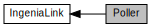
\includegraphics[width=223pt]{group__IL__POLLER}
\end{center}
\end{figure}
\subsection*{Data Structures}
\begin{DoxyCompactItemize}
\item 
struct \hyperlink{structil__poller__acq__t}{il\+\_\+poller\+\_\+acq\+\_\+t}
\begin{DoxyCompactList}\small\item\em Poller acquisition results. \end{DoxyCompactList}\end{DoxyCompactItemize}
\subsection*{Typedefs}
\begin{DoxyCompactItemize}
\item 
typedef struct il\+\_\+poller \hyperlink{group__IL__POLLER_ga896ad3836b2a1e121ce8b0c30c58d3ab}{il\+\_\+poller\+\_\+t}
\begin{DoxyCompactList}\small\item\em Ingenia\+Link poller. \end{DoxyCompactList}\end{DoxyCompactItemize}
\subsection*{Functions}
\begin{DoxyCompactItemize}
\item 
\hyperlink{common_8h_a6bb629d26c52bfe10519ba3176853f47}{I\+L\+\_\+\+E\+X\+P\+O\+RT} \hyperlink{group__IL__POLLER_ga896ad3836b2a1e121ce8b0c30c58d3ab}{il\+\_\+poller\+\_\+t} $\ast$ \hyperlink{group__IL__POLLER_gaf1a6d95123039ac685439062c34e7e54}{il\+\_\+poller\+\_\+create} (\hyperlink{group__IL__SERVO_ga3369ddfcc33492fe3a28f96cf455b13e}{il\+\_\+servo\+\_\+t} $\ast$servo, size\+\_\+t n\+\_\+ch)
\begin{DoxyCompactList}\small\item\em Create a register poller. \end{DoxyCompactList}\item 
\hyperlink{common_8h_a6bb629d26c52bfe10519ba3176853f47}{I\+L\+\_\+\+E\+X\+P\+O\+RT} void \hyperlink{group__IL__POLLER_gada8133cbba4d0212e6d5c84dab03d407}{il\+\_\+poller\+\_\+destroy} (\hyperlink{group__IL__POLLER_ga896ad3836b2a1e121ce8b0c30c58d3ab}{il\+\_\+poller\+\_\+t} $\ast$poller)
\begin{DoxyCompactList}\small\item\em Destroy a register poller. \end{DoxyCompactList}\item 
\hyperlink{common_8h_a6bb629d26c52bfe10519ba3176853f47}{I\+L\+\_\+\+E\+X\+P\+O\+RT} int \hyperlink{group__IL__POLLER_ga018f08358312c8610819a47fd9d2509f}{il\+\_\+poller\+\_\+start} (\hyperlink{group__IL__POLLER_ga896ad3836b2a1e121ce8b0c30c58d3ab}{il\+\_\+poller\+\_\+t} $\ast$poller)
\begin{DoxyCompactList}\small\item\em Start poller. \end{DoxyCompactList}\item 
\hyperlink{common_8h_a6bb629d26c52bfe10519ba3176853f47}{I\+L\+\_\+\+E\+X\+P\+O\+RT} void \hyperlink{group__IL__POLLER_ga1055384cca31fe730d07d488017c559f}{il\+\_\+poller\+\_\+stop} (\hyperlink{group__IL__POLLER_ga896ad3836b2a1e121ce8b0c30c58d3ab}{il\+\_\+poller\+\_\+t} $\ast$poller)
\begin{DoxyCompactList}\small\item\em Stop poller. \end{DoxyCompactList}\item 
\hyperlink{common_8h_a6bb629d26c52bfe10519ba3176853f47}{I\+L\+\_\+\+E\+X\+P\+O\+RT} void \hyperlink{group__IL__POLLER_ga67ccc0e92b0bb83756462d3c407d4d87}{il\+\_\+poller\+\_\+data\+\_\+get} (\hyperlink{group__IL__POLLER_ga896ad3836b2a1e121ce8b0c30c58d3ab}{il\+\_\+poller\+\_\+t} $\ast$poller, \hyperlink{structil__poller__acq__t}{il\+\_\+poller\+\_\+acq\+\_\+t} $\ast$$\ast$acq)
\begin{DoxyCompactList}\small\item\em Obtain current time and data vectors. \end{DoxyCompactList}\item 
\hyperlink{common_8h_a6bb629d26c52bfe10519ba3176853f47}{I\+L\+\_\+\+E\+X\+P\+O\+RT} int \hyperlink{group__IL__POLLER_ga90aa41e8a0ff21af9d077e522cefb205}{il\+\_\+poller\+\_\+configure} (\hyperlink{group__IL__POLLER_ga896ad3836b2a1e121ce8b0c30c58d3ab}{il\+\_\+poller\+\_\+t} $\ast$poller, unsigned int t\+\_\+s, size\+\_\+t buf\+\_\+sz)
\begin{DoxyCompactList}\small\item\em Configure poller parameters. \end{DoxyCompactList}\item 
\hyperlink{common_8h_a6bb629d26c52bfe10519ba3176853f47}{I\+L\+\_\+\+E\+X\+P\+O\+RT} int \hyperlink{group__IL__POLLER_ga615595277add47dd6966112e48e66988}{il\+\_\+poller\+\_\+ch\+\_\+configure} (\hyperlink{group__IL__POLLER_ga896ad3836b2a1e121ce8b0c30c58d3ab}{il\+\_\+poller\+\_\+t} $\ast$poller, unsigned int ch, const \hyperlink{structil__reg__t}{il\+\_\+reg\+\_\+t} $\ast$reg, const char $\ast$id)
\begin{DoxyCompactList}\small\item\em Configure a poller channel. \end{DoxyCompactList}\item 
\hyperlink{common_8h_a6bb629d26c52bfe10519ba3176853f47}{I\+L\+\_\+\+E\+X\+P\+O\+RT} int \hyperlink{group__IL__POLLER_ga1722948bea216e9bb85be820f175371d}{il\+\_\+poller\+\_\+ch\+\_\+disable} (\hyperlink{group__IL__POLLER_ga896ad3836b2a1e121ce8b0c30c58d3ab}{il\+\_\+poller\+\_\+t} $\ast$poller, unsigned int ch)
\begin{DoxyCompactList}\small\item\em Disable a poller channel. \end{DoxyCompactList}\item 
\hyperlink{common_8h_a6bb629d26c52bfe10519ba3176853f47}{I\+L\+\_\+\+E\+X\+P\+O\+RT} int \hyperlink{group__IL__POLLER_gac58b529d800310d6f68f00f195fab9c1}{il\+\_\+poller\+\_\+ch\+\_\+disable\+\_\+all} (\hyperlink{group__IL__POLLER_ga896ad3836b2a1e121ce8b0c30c58d3ab}{il\+\_\+poller\+\_\+t} $\ast$poller)
\begin{DoxyCompactList}\small\item\em Disable all poller channels. \end{DoxyCompactList}\end{DoxyCompactItemize}


\subsection{Detailed Description}


\subsection{Typedef Documentation}
\index{Poller@{Poller}!il\+\_\+poller\+\_\+t@{il\+\_\+poller\+\_\+t}}
\index{il\+\_\+poller\+\_\+t@{il\+\_\+poller\+\_\+t}!Poller@{Poller}}
\subsubsection[{\texorpdfstring{il\+\_\+poller\+\_\+t}{il_poller_t}}]{\setlength{\rightskip}{0pt plus 5cm}typedef struct il\+\_\+poller {\bf il\+\_\+poller\+\_\+t}}\hypertarget{group__IL__POLLER_ga896ad3836b2a1e121ce8b0c30c58d3ab}{}\label{group__IL__POLLER_ga896ad3836b2a1e121ce8b0c30c58d3ab}


Ingenia\+Link poller. 



\subsection{Function Documentation}
\index{Poller@{Poller}!il\+\_\+poller\+\_\+ch\+\_\+configure@{il\+\_\+poller\+\_\+ch\+\_\+configure}}
\index{il\+\_\+poller\+\_\+ch\+\_\+configure@{il\+\_\+poller\+\_\+ch\+\_\+configure}!Poller@{Poller}}
\subsubsection[{\texorpdfstring{il\+\_\+poller\+\_\+ch\+\_\+configure(il\+\_\+poller\+\_\+t $\ast$poller, unsigned int ch, const il\+\_\+reg\+\_\+t $\ast$reg, const char $\ast$id)}{il_poller_ch_configure(il_poller_t *poller, unsigned int ch, const il_reg_t *reg, const char *id)}}]{\setlength{\rightskip}{0pt plus 5cm}{\bf I\+L\+\_\+\+E\+X\+P\+O\+RT} int il\+\_\+poller\+\_\+ch\+\_\+configure (
\begin{DoxyParamCaption}
\item[{{\bf il\+\_\+poller\+\_\+t} $\ast$}]{poller, }
\item[{unsigned int}]{ch, }
\item[{const {\bf il\+\_\+reg\+\_\+t} $\ast$}]{reg, }
\item[{const char $\ast$}]{id}
\end{DoxyParamCaption}
)}\hypertarget{group__IL__POLLER_ga615595277add47dd6966112e48e66988}{}\label{group__IL__POLLER_ga615595277add47dd6966112e48e66988}


Configure a poller channel. 


\begin{DoxyParams}[1]{Parameters}
\mbox{\tt in}  & {\em poller} & Poller instance. \\
\hline
\mbox{\tt in}  & {\em ch} & Channel. \\
\hline
\mbox{\tt in}  & {\em reg} & Register (pre-\/defined) to be polled on this channel. \\
\hline
\mbox{\tt in}  & {\em id} & Register ID to be polled on this channel.\\
\hline
\end{DoxyParams}
\begin{DoxyReturn}{Returns}
0 on success, error code otherwise. 
\end{DoxyReturn}
\begin{Desc}
\item[Examples\+: ]\par
\hyperlink{motion_8c-example}{motion.\+c}.\end{Desc}
\index{Poller@{Poller}!il\+\_\+poller\+\_\+ch\+\_\+disable@{il\+\_\+poller\+\_\+ch\+\_\+disable}}
\index{il\+\_\+poller\+\_\+ch\+\_\+disable@{il\+\_\+poller\+\_\+ch\+\_\+disable}!Poller@{Poller}}
\subsubsection[{\texorpdfstring{il\+\_\+poller\+\_\+ch\+\_\+disable(il\+\_\+poller\+\_\+t $\ast$poller, unsigned int ch)}{il_poller_ch_disable(il_poller_t *poller, unsigned int ch)}}]{\setlength{\rightskip}{0pt plus 5cm}{\bf I\+L\+\_\+\+E\+X\+P\+O\+RT} int il\+\_\+poller\+\_\+ch\+\_\+disable (
\begin{DoxyParamCaption}
\item[{{\bf il\+\_\+poller\+\_\+t} $\ast$}]{poller, }
\item[{unsigned int}]{ch}
\end{DoxyParamCaption}
)}\hypertarget{group__IL__POLLER_ga1722948bea216e9bb85be820f175371d}{}\label{group__IL__POLLER_ga1722948bea216e9bb85be820f175371d}


Disable a poller channel. 


\begin{DoxyParams}[1]{Parameters}
\mbox{\tt in}  & {\em poller} & Poller instance. \\
\hline
\mbox{\tt in}  & {\em ch} & Channel.\\
\hline
\end{DoxyParams}
\begin{DoxyReturn}{Returns}
0 on success, error code otherwise. 
\end{DoxyReturn}
\index{Poller@{Poller}!il\+\_\+poller\+\_\+ch\+\_\+disable\+\_\+all@{il\+\_\+poller\+\_\+ch\+\_\+disable\+\_\+all}}
\index{il\+\_\+poller\+\_\+ch\+\_\+disable\+\_\+all@{il\+\_\+poller\+\_\+ch\+\_\+disable\+\_\+all}!Poller@{Poller}}
\subsubsection[{\texorpdfstring{il\+\_\+poller\+\_\+ch\+\_\+disable\+\_\+all(il\+\_\+poller\+\_\+t $\ast$poller)}{il_poller_ch_disable_all(il_poller_t *poller)}}]{\setlength{\rightskip}{0pt plus 5cm}{\bf I\+L\+\_\+\+E\+X\+P\+O\+RT} int il\+\_\+poller\+\_\+ch\+\_\+disable\+\_\+all (
\begin{DoxyParamCaption}
\item[{{\bf il\+\_\+poller\+\_\+t} $\ast$}]{poller}
\end{DoxyParamCaption}
)}\hypertarget{group__IL__POLLER_gac58b529d800310d6f68f00f195fab9c1}{}\label{group__IL__POLLER_gac58b529d800310d6f68f00f195fab9c1}


Disable all poller channels. 


\begin{DoxyParams}[1]{Parameters}
\mbox{\tt in}  & {\em poller} & Poller instance.\\
\hline
\end{DoxyParams}
\begin{DoxyReturn}{Returns}
0 on success, error code otherwise. 
\end{DoxyReturn}
\index{Poller@{Poller}!il\+\_\+poller\+\_\+configure@{il\+\_\+poller\+\_\+configure}}
\index{il\+\_\+poller\+\_\+configure@{il\+\_\+poller\+\_\+configure}!Poller@{Poller}}
\subsubsection[{\texorpdfstring{il\+\_\+poller\+\_\+configure(il\+\_\+poller\+\_\+t $\ast$poller, unsigned int t\+\_\+s, size\+\_\+t buf\+\_\+sz)}{il_poller_configure(il_poller_t *poller, unsigned int t_s, size_t buf_sz)}}]{\setlength{\rightskip}{0pt plus 5cm}{\bf I\+L\+\_\+\+E\+X\+P\+O\+RT} int il\+\_\+poller\+\_\+configure (
\begin{DoxyParamCaption}
\item[{{\bf il\+\_\+poller\+\_\+t} $\ast$}]{poller, }
\item[{unsigned int}]{t\+\_\+s, }
\item[{size\+\_\+t}]{buf\+\_\+sz}
\end{DoxyParamCaption}
)}\hypertarget{group__IL__POLLER_ga90aa41e8a0ff21af9d077e522cefb205}{}\label{group__IL__POLLER_ga90aa41e8a0ff21af9d077e522cefb205}


Configure poller parameters. 

\begin{DoxyNote}{Note}

\begin{DoxyItemize}
\item The maximum stable polling rate is $\sim$500 Hz (2 ms) for a single register when the servo is enabled.
\item The buffer size must be set according to your application needs. It should be large enough so that it can store all samples collected between subsequent calls to {\ttfamily il\+\_\+poller\+\_\+data\+\_\+get}.
\end{DoxyItemize}
\end{DoxyNote}

\begin{DoxyParams}[1]{Parameters}
\mbox{\tt in}  & {\em poller} & Poller instance. \\
\hline
\mbox{\tt in}  & {\em t\+\_\+s} & Sampling period (ms). \\
\hline
\mbox{\tt in}  & {\em buf\+\_\+sz} & Buffer size.\\
\hline
\end{DoxyParams}
\begin{DoxyReturn}{Returns}
0 on success, error code otherwise. 
\end{DoxyReturn}
\begin{Desc}
\item[Examples\+: ]\par
\hyperlink{motion_8c-example}{motion.\+c}.\end{Desc}
\index{Poller@{Poller}!il\+\_\+poller\+\_\+create@{il\+\_\+poller\+\_\+create}}
\index{il\+\_\+poller\+\_\+create@{il\+\_\+poller\+\_\+create}!Poller@{Poller}}
\subsubsection[{\texorpdfstring{il\+\_\+poller\+\_\+create(il\+\_\+servo\+\_\+t $\ast$servo, size\+\_\+t n\+\_\+ch)}{il_poller_create(il_servo_t *servo, size_t n_ch)}}]{\setlength{\rightskip}{0pt plus 5cm}{\bf I\+L\+\_\+\+E\+X\+P\+O\+RT} {\bf il\+\_\+poller\+\_\+t}$\ast$ il\+\_\+poller\+\_\+create (
\begin{DoxyParamCaption}
\item[{{\bf il\+\_\+servo\+\_\+t} $\ast$}]{servo, }
\item[{size\+\_\+t}]{n\+\_\+ch}
\end{DoxyParamCaption}
)}\hypertarget{group__IL__POLLER_gaf1a6d95123039ac685439062c34e7e54}{}\label{group__IL__POLLER_gaf1a6d95123039ac685439062c34e7e54}


Create a register poller. 


\begin{DoxyParams}[1]{Parameters}
\mbox{\tt in}  & {\em servo} & Ingenia\+Link servo. \\
\hline
\mbox{\tt in}  & {\em n\+\_\+ch} & Number of channels.\\
\hline
\end{DoxyParams}
\begin{DoxyReturn}{Returns}
Poller instance (N\+U\+LL if it could not be created). 
\end{DoxyReturn}
\begin{Desc}
\item[Examples\+: ]\par
\hyperlink{motion_8c-example}{motion.\+c}.\end{Desc}
\index{Poller@{Poller}!il\+\_\+poller\+\_\+data\+\_\+get@{il\+\_\+poller\+\_\+data\+\_\+get}}
\index{il\+\_\+poller\+\_\+data\+\_\+get@{il\+\_\+poller\+\_\+data\+\_\+get}!Poller@{Poller}}
\subsubsection[{\texorpdfstring{il\+\_\+poller\+\_\+data\+\_\+get(il\+\_\+poller\+\_\+t $\ast$poller, il\+\_\+poller\+\_\+acq\+\_\+t $\ast$$\ast$acq)}{il_poller_data_get(il_poller_t *poller, il_poller_acq_t **acq)}}]{\setlength{\rightskip}{0pt plus 5cm}{\bf I\+L\+\_\+\+E\+X\+P\+O\+RT} void il\+\_\+poller\+\_\+data\+\_\+get (
\begin{DoxyParamCaption}
\item[{{\bf il\+\_\+poller\+\_\+t} $\ast$}]{poller, }
\item[{{\bf il\+\_\+poller\+\_\+acq\+\_\+t} $\ast$$\ast$}]{acq}
\end{DoxyParamCaption}
)}\hypertarget{group__IL__POLLER_ga67ccc0e92b0bb83756462d3c407d4d87}{}\label{group__IL__POLLER_ga67ccc0e92b0bb83756462d3c407d4d87}


Obtain current time and data vectors. 

\begin{DoxyNote}{Note}
The obtained acquisition data can be used until the next call to this function.
\end{DoxyNote}

\begin{DoxyParams}[1]{Parameters}
\mbox{\tt in}  & {\em poller} & Poller instance. \\
\hline
\mbox{\tt out}  & {\em acq} & Where the acquisition results will be left. \\
\hline
\end{DoxyParams}
\begin{Desc}
\item[Examples\+: ]\par
\hyperlink{motion_8c-example}{motion.\+c}.\end{Desc}
\index{Poller@{Poller}!il\+\_\+poller\+\_\+destroy@{il\+\_\+poller\+\_\+destroy}}
\index{il\+\_\+poller\+\_\+destroy@{il\+\_\+poller\+\_\+destroy}!Poller@{Poller}}
\subsubsection[{\texorpdfstring{il\+\_\+poller\+\_\+destroy(il\+\_\+poller\+\_\+t $\ast$poller)}{il_poller_destroy(il_poller_t *poller)}}]{\setlength{\rightskip}{0pt plus 5cm}{\bf I\+L\+\_\+\+E\+X\+P\+O\+RT} void il\+\_\+poller\+\_\+destroy (
\begin{DoxyParamCaption}
\item[{{\bf il\+\_\+poller\+\_\+t} $\ast$}]{poller}
\end{DoxyParamCaption}
)}\hypertarget{group__IL__POLLER_gada8133cbba4d0212e6d5c84dab03d407}{}\label{group__IL__POLLER_gada8133cbba4d0212e6d5c84dab03d407}


Destroy a register poller. 


\begin{DoxyParams}[1]{Parameters}
\mbox{\tt in}  & {\em poller} & Poller instance. \\
\hline
\end{DoxyParams}
\begin{Desc}
\item[Examples\+: ]\par
\hyperlink{motion_8c-example}{motion.\+c}.\end{Desc}
\index{Poller@{Poller}!il\+\_\+poller\+\_\+start@{il\+\_\+poller\+\_\+start}}
\index{il\+\_\+poller\+\_\+start@{il\+\_\+poller\+\_\+start}!Poller@{Poller}}
\subsubsection[{\texorpdfstring{il\+\_\+poller\+\_\+start(il\+\_\+poller\+\_\+t $\ast$poller)}{il_poller_start(il_poller_t *poller)}}]{\setlength{\rightskip}{0pt plus 5cm}{\bf I\+L\+\_\+\+E\+X\+P\+O\+RT} int il\+\_\+poller\+\_\+start (
\begin{DoxyParamCaption}
\item[{{\bf il\+\_\+poller\+\_\+t} $\ast$}]{poller}
\end{DoxyParamCaption}
)}\hypertarget{group__IL__POLLER_ga018f08358312c8610819a47fd9d2509f}{}\label{group__IL__POLLER_ga018f08358312c8610819a47fd9d2509f}


Start poller. 


\begin{DoxyParams}[1]{Parameters}
\mbox{\tt in}  & {\em poller} & Poller instance.\\
\hline
\end{DoxyParams}
\begin{DoxyReturn}{Returns}
0 on success, error code otherwise. 
\end{DoxyReturn}
\begin{Desc}
\item[Examples\+: ]\par
\hyperlink{motion_8c-example}{motion.\+c}.\end{Desc}
\index{Poller@{Poller}!il\+\_\+poller\+\_\+stop@{il\+\_\+poller\+\_\+stop}}
\index{il\+\_\+poller\+\_\+stop@{il\+\_\+poller\+\_\+stop}!Poller@{Poller}}
\subsubsection[{\texorpdfstring{il\+\_\+poller\+\_\+stop(il\+\_\+poller\+\_\+t $\ast$poller)}{il_poller_stop(il_poller_t *poller)}}]{\setlength{\rightskip}{0pt plus 5cm}{\bf I\+L\+\_\+\+E\+X\+P\+O\+RT} void il\+\_\+poller\+\_\+stop (
\begin{DoxyParamCaption}
\item[{{\bf il\+\_\+poller\+\_\+t} $\ast$}]{poller}
\end{DoxyParamCaption}
)}\hypertarget{group__IL__POLLER_ga1055384cca31fe730d07d488017c559f}{}\label{group__IL__POLLER_ga1055384cca31fe730d07d488017c559f}


Stop poller. 


\begin{DoxyParams}[1]{Parameters}
\mbox{\tt in}  & {\em poller} & Poller instance. \\
\hline
\end{DoxyParams}
\begin{Desc}
\item[Examples\+: ]\par
\hyperlink{motion_8c-example}{motion.\+c}.\end{Desc}

\hypertarget{group__IL__REGS}{}\section{Registers}
\label{group__IL__REGS}\index{Registers@{Registers}}
Collaboration diagram for Registers\+:\nopagebreak
\begin{figure}[H]
\begin{center}
\leavevmode
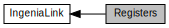
\includegraphics[width=241pt]{group__IL__REGS}
\end{center}
\end{figure}
\subsection*{Data Structures}
\begin{DoxyCompactItemize}
\item 
union \hyperlink{unionil__reg__limit__t}{il\+\_\+reg\+\_\+limit\+\_\+t}
\begin{DoxyCompactList}\small\item\em Limits. \end{DoxyCompactList}\item 
struct \hyperlink{structil__reg__range__t}{il\+\_\+reg\+\_\+range\+\_\+t}
\begin{DoxyCompactList}\small\item\em Range. \end{DoxyCompactList}\item 
struct \hyperlink{structil__reg__t}{il\+\_\+reg\+\_\+t}
\begin{DoxyCompactList}\small\item\em Register. \end{DoxyCompactList}\end{DoxyCompactItemize}
\subsection*{Enumerations}
\begin{DoxyCompactItemize}
\item 
enum \hyperlink{group__IL__REGS_gaddd7edef254d348f2e8a48c40840cdd6}{il\+\_\+reg\+\_\+dtype\+\_\+t} \{ \\*
\hyperlink{group__IL__REGS_ggaddd7edef254d348f2e8a48c40840cdd6afebd31a475c6cb6b6c9ac200fd90a09b}{I\+L\+\_\+\+R\+E\+G\+\_\+\+D\+T\+Y\+P\+E\+\_\+\+U8}, 
\hyperlink{group__IL__REGS_ggaddd7edef254d348f2e8a48c40840cdd6a4d3f76f5e0e716d7b358d819691e834a}{I\+L\+\_\+\+R\+E\+G\+\_\+\+D\+T\+Y\+P\+E\+\_\+\+S8}, 
\hyperlink{group__IL__REGS_ggaddd7edef254d348f2e8a48c40840cdd6a4776d418653151a6cadd41574d631bfa}{I\+L\+\_\+\+R\+E\+G\+\_\+\+D\+T\+Y\+P\+E\+\_\+\+U16}, 
\hyperlink{group__IL__REGS_ggaddd7edef254d348f2e8a48c40840cdd6a3eb3b654856f84234168d58355e83a85}{I\+L\+\_\+\+R\+E\+G\+\_\+\+D\+T\+Y\+P\+E\+\_\+\+S16}, 
\\*
\hyperlink{group__IL__REGS_ggaddd7edef254d348f2e8a48c40840cdd6a3d299c6c4bbda29b3286a3483271ee90}{I\+L\+\_\+\+R\+E\+G\+\_\+\+D\+T\+Y\+P\+E\+\_\+\+U32}, 
\hyperlink{group__IL__REGS_ggaddd7edef254d348f2e8a48c40840cdd6aaf16d13caf933d3e002054de7a0f1c48}{I\+L\+\_\+\+R\+E\+G\+\_\+\+D\+T\+Y\+P\+E\+\_\+\+S32}, 
\hyperlink{group__IL__REGS_ggaddd7edef254d348f2e8a48c40840cdd6a5a0f02c573b8800ee8f113160ce93712}{I\+L\+\_\+\+R\+E\+G\+\_\+\+D\+T\+Y\+P\+E\+\_\+\+U64}, 
\hyperlink{group__IL__REGS_ggaddd7edef254d348f2e8a48c40840cdd6a37398082dc9828038d3403ca24a28d5a}{I\+L\+\_\+\+R\+E\+G\+\_\+\+D\+T\+Y\+P\+E\+\_\+\+S64}, 
\\*
\hyperlink{group__IL__REGS_ggaddd7edef254d348f2e8a48c40840cdd6a07e3bbcf6a1d00d8f62887e41b529239}{I\+L\+\_\+\+R\+E\+G\+\_\+\+D\+T\+Y\+P\+E\+\_\+\+F\+L\+O\+AT}, 
\hyperlink{group__IL__REGS_ggaddd7edef254d348f2e8a48c40840cdd6aeb15ea8dd9961e96edebfc3d0f36fbd3}{I\+L\+\_\+\+R\+E\+G\+\_\+\+D\+T\+Y\+P\+E\+\_\+\+S\+TR}
 \}\begin{DoxyCompactList}\small\item\em Register data type. \end{DoxyCompactList}
\item 
enum \hyperlink{group__IL__REGS_ga4c623bd7d0d5f059dd91949c6948147e}{il\+\_\+reg\+\_\+access\+\_\+t} \{ \hyperlink{group__IL__REGS_gga4c623bd7d0d5f059dd91949c6948147eafa388eb7ec6166ba6a59d0d665f3ac53}{I\+L\+\_\+\+R\+E\+G\+\_\+\+A\+C\+C\+E\+S\+S\+\_\+\+RW}, 
\hyperlink{group__IL__REGS_gga4c623bd7d0d5f059dd91949c6948147ea12dabd43c525dfea5fb20914711168b8}{I\+L\+\_\+\+R\+E\+G\+\_\+\+A\+C\+C\+E\+S\+S\+\_\+\+RO}, 
\hyperlink{group__IL__REGS_gga4c623bd7d0d5f059dd91949c6948147eadb0026436ae70de8a60920c1085561bb}{I\+L\+\_\+\+R\+E\+G\+\_\+\+A\+C\+C\+E\+S\+S\+\_\+\+WO}
 \}\begin{DoxyCompactList}\small\item\em Register access. \end{DoxyCompactList}
\item 
enum \hyperlink{group__IL__REGS_ga37538453e5c3d84733c628987a579590}{il\+\_\+reg\+\_\+phy\+\_\+t} \{ \\*
\hyperlink{group__IL__REGS_gga37538453e5c3d84733c628987a579590a34d96ac8a7b9afc02256a03d5a464822}{I\+L\+\_\+\+R\+E\+G\+\_\+\+P\+H\+Y\+\_\+\+N\+O\+NE}, 
\hyperlink{group__IL__REGS_gga37538453e5c3d84733c628987a579590a799176bbdcea555949cd68969361bc8f}{I\+L\+\_\+\+R\+E\+G\+\_\+\+P\+H\+Y\+\_\+\+T\+O\+R\+Q\+UE}, 
\hyperlink{group__IL__REGS_gga37538453e5c3d84733c628987a579590ad7bdcaae981dfbbd28c46bed55f947ac}{I\+L\+\_\+\+R\+E\+G\+\_\+\+P\+H\+Y\+\_\+\+P\+OS}, 
\hyperlink{group__IL__REGS_gga37538453e5c3d84733c628987a579590aea1c9cf80466e862af6a3a6f687550ef}{I\+L\+\_\+\+R\+E\+G\+\_\+\+P\+H\+Y\+\_\+\+V\+EL}, 
\\*
\hyperlink{group__IL__REGS_gga37538453e5c3d84733c628987a579590a3dc604058c640ad2997c5d4a1ad37b97}{I\+L\+\_\+\+R\+E\+G\+\_\+\+P\+H\+Y\+\_\+\+A\+CC}, 
\hyperlink{group__IL__REGS_gga37538453e5c3d84733c628987a579590a99385428e977da83262b2ad47bcfc8f0}{I\+L\+\_\+\+R\+E\+G\+\_\+\+P\+H\+Y\+\_\+\+V\+O\+L\+T\+\_\+\+R\+EL}, 
\hyperlink{group__IL__REGS_gga37538453e5c3d84733c628987a579590a0cad6fc9aa35ccf3b78d695f9a446e2e}{I\+L\+\_\+\+R\+E\+G\+\_\+\+P\+H\+Y\+\_\+\+R\+AD}
 \}\begin{DoxyCompactList}\small\item\em Register physical units type. \end{DoxyCompactList}
\end{DoxyCompactItemize}


\subsection{Detailed Description}


\subsection{Enumeration Type Documentation}
\index{Registers@{Registers}!il\+\_\+reg\+\_\+access\+\_\+t@{il\+\_\+reg\+\_\+access\+\_\+t}}
\index{il\+\_\+reg\+\_\+access\+\_\+t@{il\+\_\+reg\+\_\+access\+\_\+t}!Registers@{Registers}}
\subsubsection[{\texorpdfstring{il\+\_\+reg\+\_\+access\+\_\+t}{il_reg_access_t}}]{\setlength{\rightskip}{0pt plus 5cm}enum {\bf il\+\_\+reg\+\_\+access\+\_\+t}}\hypertarget{group__IL__REGS_ga4c623bd7d0d5f059dd91949c6948147e}{}\label{group__IL__REGS_ga4c623bd7d0d5f059dd91949c6948147e}


Register access. 

\begin{Desc}
\item[Enumerator]\par
\begin{description}
\index{I\+L\+\_\+\+R\+E\+G\+\_\+\+A\+C\+C\+E\+S\+S\+\_\+\+RW@{I\+L\+\_\+\+R\+E\+G\+\_\+\+A\+C\+C\+E\+S\+S\+\_\+\+RW}!Registers@{Registers}}\index{Registers@{Registers}!I\+L\+\_\+\+R\+E\+G\+\_\+\+A\+C\+C\+E\+S\+S\+\_\+\+RW@{I\+L\+\_\+\+R\+E\+G\+\_\+\+A\+C\+C\+E\+S\+S\+\_\+\+RW}}\item[{\em 
I\+L\+\_\+\+R\+E\+G\+\_\+\+A\+C\+C\+E\+S\+S\+\_\+\+RW\hypertarget{group__IL__REGS_gga4c623bd7d0d5f059dd91949c6948147eafa388eb7ec6166ba6a59d0d665f3ac53}{}\label{group__IL__REGS_gga4c623bd7d0d5f059dd91949c6948147eafa388eb7ec6166ba6a59d0d665f3ac53}
}]Read/\+Write. \index{I\+L\+\_\+\+R\+E\+G\+\_\+\+A\+C\+C\+E\+S\+S\+\_\+\+RO@{I\+L\+\_\+\+R\+E\+G\+\_\+\+A\+C\+C\+E\+S\+S\+\_\+\+RO}!Registers@{Registers}}\index{Registers@{Registers}!I\+L\+\_\+\+R\+E\+G\+\_\+\+A\+C\+C\+E\+S\+S\+\_\+\+RO@{I\+L\+\_\+\+R\+E\+G\+\_\+\+A\+C\+C\+E\+S\+S\+\_\+\+RO}}\item[{\em 
I\+L\+\_\+\+R\+E\+G\+\_\+\+A\+C\+C\+E\+S\+S\+\_\+\+RO\hypertarget{group__IL__REGS_gga4c623bd7d0d5f059dd91949c6948147ea12dabd43c525dfea5fb20914711168b8}{}\label{group__IL__REGS_gga4c623bd7d0d5f059dd91949c6948147ea12dabd43c525dfea5fb20914711168b8}
}]Read only. \index{I\+L\+\_\+\+R\+E\+G\+\_\+\+A\+C\+C\+E\+S\+S\+\_\+\+WO@{I\+L\+\_\+\+R\+E\+G\+\_\+\+A\+C\+C\+E\+S\+S\+\_\+\+WO}!Registers@{Registers}}\index{Registers@{Registers}!I\+L\+\_\+\+R\+E\+G\+\_\+\+A\+C\+C\+E\+S\+S\+\_\+\+WO@{I\+L\+\_\+\+R\+E\+G\+\_\+\+A\+C\+C\+E\+S\+S\+\_\+\+WO}}\item[{\em 
I\+L\+\_\+\+R\+E\+G\+\_\+\+A\+C\+C\+E\+S\+S\+\_\+\+WO\hypertarget{group__IL__REGS_gga4c623bd7d0d5f059dd91949c6948147eadb0026436ae70de8a60920c1085561bb}{}\label{group__IL__REGS_gga4c623bd7d0d5f059dd91949c6948147eadb0026436ae70de8a60920c1085561bb}
}]Write only. \end{description}
\end{Desc}
\index{Registers@{Registers}!il\+\_\+reg\+\_\+dtype\+\_\+t@{il\+\_\+reg\+\_\+dtype\+\_\+t}}
\index{il\+\_\+reg\+\_\+dtype\+\_\+t@{il\+\_\+reg\+\_\+dtype\+\_\+t}!Registers@{Registers}}
\subsubsection[{\texorpdfstring{il\+\_\+reg\+\_\+dtype\+\_\+t}{il_reg_dtype_t}}]{\setlength{\rightskip}{0pt plus 5cm}enum {\bf il\+\_\+reg\+\_\+dtype\+\_\+t}}\hypertarget{group__IL__REGS_gaddd7edef254d348f2e8a48c40840cdd6}{}\label{group__IL__REGS_gaddd7edef254d348f2e8a48c40840cdd6}


Register data type. 

\begin{Desc}
\item[Enumerator]\par
\begin{description}
\index{I\+L\+\_\+\+R\+E\+G\+\_\+\+D\+T\+Y\+P\+E\+\_\+\+U8@{I\+L\+\_\+\+R\+E\+G\+\_\+\+D\+T\+Y\+P\+E\+\_\+\+U8}!Registers@{Registers}}\index{Registers@{Registers}!I\+L\+\_\+\+R\+E\+G\+\_\+\+D\+T\+Y\+P\+E\+\_\+\+U8@{I\+L\+\_\+\+R\+E\+G\+\_\+\+D\+T\+Y\+P\+E\+\_\+\+U8}}\item[{\em 
I\+L\+\_\+\+R\+E\+G\+\_\+\+D\+T\+Y\+P\+E\+\_\+\+U8\hypertarget{group__IL__REGS_ggaddd7edef254d348f2e8a48c40840cdd6afebd31a475c6cb6b6c9ac200fd90a09b}{}\label{group__IL__REGS_ggaddd7edef254d348f2e8a48c40840cdd6afebd31a475c6cb6b6c9ac200fd90a09b}
}]Unsigned 8-\/bit integer. \index{I\+L\+\_\+\+R\+E\+G\+\_\+\+D\+T\+Y\+P\+E\+\_\+\+S8@{I\+L\+\_\+\+R\+E\+G\+\_\+\+D\+T\+Y\+P\+E\+\_\+\+S8}!Registers@{Registers}}\index{Registers@{Registers}!I\+L\+\_\+\+R\+E\+G\+\_\+\+D\+T\+Y\+P\+E\+\_\+\+S8@{I\+L\+\_\+\+R\+E\+G\+\_\+\+D\+T\+Y\+P\+E\+\_\+\+S8}}\item[{\em 
I\+L\+\_\+\+R\+E\+G\+\_\+\+D\+T\+Y\+P\+E\+\_\+\+S8\hypertarget{group__IL__REGS_ggaddd7edef254d348f2e8a48c40840cdd6a4d3f76f5e0e716d7b358d819691e834a}{}\label{group__IL__REGS_ggaddd7edef254d348f2e8a48c40840cdd6a4d3f76f5e0e716d7b358d819691e834a}
}]Signed 8-\/bit integer. \index{I\+L\+\_\+\+R\+E\+G\+\_\+\+D\+T\+Y\+P\+E\+\_\+\+U16@{I\+L\+\_\+\+R\+E\+G\+\_\+\+D\+T\+Y\+P\+E\+\_\+\+U16}!Registers@{Registers}}\index{Registers@{Registers}!I\+L\+\_\+\+R\+E\+G\+\_\+\+D\+T\+Y\+P\+E\+\_\+\+U16@{I\+L\+\_\+\+R\+E\+G\+\_\+\+D\+T\+Y\+P\+E\+\_\+\+U16}}\item[{\em 
I\+L\+\_\+\+R\+E\+G\+\_\+\+D\+T\+Y\+P\+E\+\_\+\+U16\hypertarget{group__IL__REGS_ggaddd7edef254d348f2e8a48c40840cdd6a4776d418653151a6cadd41574d631bfa}{}\label{group__IL__REGS_ggaddd7edef254d348f2e8a48c40840cdd6a4776d418653151a6cadd41574d631bfa}
}]Unsigned 16-\/bit integer. \index{I\+L\+\_\+\+R\+E\+G\+\_\+\+D\+T\+Y\+P\+E\+\_\+\+S16@{I\+L\+\_\+\+R\+E\+G\+\_\+\+D\+T\+Y\+P\+E\+\_\+\+S16}!Registers@{Registers}}\index{Registers@{Registers}!I\+L\+\_\+\+R\+E\+G\+\_\+\+D\+T\+Y\+P\+E\+\_\+\+S16@{I\+L\+\_\+\+R\+E\+G\+\_\+\+D\+T\+Y\+P\+E\+\_\+\+S16}}\item[{\em 
I\+L\+\_\+\+R\+E\+G\+\_\+\+D\+T\+Y\+P\+E\+\_\+\+S16\hypertarget{group__IL__REGS_ggaddd7edef254d348f2e8a48c40840cdd6a3eb3b654856f84234168d58355e83a85}{}\label{group__IL__REGS_ggaddd7edef254d348f2e8a48c40840cdd6a3eb3b654856f84234168d58355e83a85}
}]Signed 16-\/bit integer. \index{I\+L\+\_\+\+R\+E\+G\+\_\+\+D\+T\+Y\+P\+E\+\_\+\+U32@{I\+L\+\_\+\+R\+E\+G\+\_\+\+D\+T\+Y\+P\+E\+\_\+\+U32}!Registers@{Registers}}\index{Registers@{Registers}!I\+L\+\_\+\+R\+E\+G\+\_\+\+D\+T\+Y\+P\+E\+\_\+\+U32@{I\+L\+\_\+\+R\+E\+G\+\_\+\+D\+T\+Y\+P\+E\+\_\+\+U32}}\item[{\em 
I\+L\+\_\+\+R\+E\+G\+\_\+\+D\+T\+Y\+P\+E\+\_\+\+U32\hypertarget{group__IL__REGS_ggaddd7edef254d348f2e8a48c40840cdd6a3d299c6c4bbda29b3286a3483271ee90}{}\label{group__IL__REGS_ggaddd7edef254d348f2e8a48c40840cdd6a3d299c6c4bbda29b3286a3483271ee90}
}]Unsigned 32-\/bit integer. \index{I\+L\+\_\+\+R\+E\+G\+\_\+\+D\+T\+Y\+P\+E\+\_\+\+S32@{I\+L\+\_\+\+R\+E\+G\+\_\+\+D\+T\+Y\+P\+E\+\_\+\+S32}!Registers@{Registers}}\index{Registers@{Registers}!I\+L\+\_\+\+R\+E\+G\+\_\+\+D\+T\+Y\+P\+E\+\_\+\+S32@{I\+L\+\_\+\+R\+E\+G\+\_\+\+D\+T\+Y\+P\+E\+\_\+\+S32}}\item[{\em 
I\+L\+\_\+\+R\+E\+G\+\_\+\+D\+T\+Y\+P\+E\+\_\+\+S32\hypertarget{group__IL__REGS_ggaddd7edef254d348f2e8a48c40840cdd6aaf16d13caf933d3e002054de7a0f1c48}{}\label{group__IL__REGS_ggaddd7edef254d348f2e8a48c40840cdd6aaf16d13caf933d3e002054de7a0f1c48}
}]Signed 32-\/bit integer. \index{I\+L\+\_\+\+R\+E\+G\+\_\+\+D\+T\+Y\+P\+E\+\_\+\+U64@{I\+L\+\_\+\+R\+E\+G\+\_\+\+D\+T\+Y\+P\+E\+\_\+\+U64}!Registers@{Registers}}\index{Registers@{Registers}!I\+L\+\_\+\+R\+E\+G\+\_\+\+D\+T\+Y\+P\+E\+\_\+\+U64@{I\+L\+\_\+\+R\+E\+G\+\_\+\+D\+T\+Y\+P\+E\+\_\+\+U64}}\item[{\em 
I\+L\+\_\+\+R\+E\+G\+\_\+\+D\+T\+Y\+P\+E\+\_\+\+U64\hypertarget{group__IL__REGS_ggaddd7edef254d348f2e8a48c40840cdd6a5a0f02c573b8800ee8f113160ce93712}{}\label{group__IL__REGS_ggaddd7edef254d348f2e8a48c40840cdd6a5a0f02c573b8800ee8f113160ce93712}
}]Unsigned 64-\/bit integer. \index{I\+L\+\_\+\+R\+E\+G\+\_\+\+D\+T\+Y\+P\+E\+\_\+\+S64@{I\+L\+\_\+\+R\+E\+G\+\_\+\+D\+T\+Y\+P\+E\+\_\+\+S64}!Registers@{Registers}}\index{Registers@{Registers}!I\+L\+\_\+\+R\+E\+G\+\_\+\+D\+T\+Y\+P\+E\+\_\+\+S64@{I\+L\+\_\+\+R\+E\+G\+\_\+\+D\+T\+Y\+P\+E\+\_\+\+S64}}\item[{\em 
I\+L\+\_\+\+R\+E\+G\+\_\+\+D\+T\+Y\+P\+E\+\_\+\+S64\hypertarget{group__IL__REGS_ggaddd7edef254d348f2e8a48c40840cdd6a37398082dc9828038d3403ca24a28d5a}{}\label{group__IL__REGS_ggaddd7edef254d348f2e8a48c40840cdd6a37398082dc9828038d3403ca24a28d5a}
}]Signed 64-\/bit integer. \index{I\+L\+\_\+\+R\+E\+G\+\_\+\+D\+T\+Y\+P\+E\+\_\+\+F\+L\+O\+AT@{I\+L\+\_\+\+R\+E\+G\+\_\+\+D\+T\+Y\+P\+E\+\_\+\+F\+L\+O\+AT}!Registers@{Registers}}\index{Registers@{Registers}!I\+L\+\_\+\+R\+E\+G\+\_\+\+D\+T\+Y\+P\+E\+\_\+\+F\+L\+O\+AT@{I\+L\+\_\+\+R\+E\+G\+\_\+\+D\+T\+Y\+P\+E\+\_\+\+F\+L\+O\+AT}}\item[{\em 
I\+L\+\_\+\+R\+E\+G\+\_\+\+D\+T\+Y\+P\+E\+\_\+\+F\+L\+O\+AT\hypertarget{group__IL__REGS_ggaddd7edef254d348f2e8a48c40840cdd6a07e3bbcf6a1d00d8f62887e41b529239}{}\label{group__IL__REGS_ggaddd7edef254d348f2e8a48c40840cdd6a07e3bbcf6a1d00d8f62887e41b529239}
}]Float. \index{I\+L\+\_\+\+R\+E\+G\+\_\+\+D\+T\+Y\+P\+E\+\_\+\+S\+TR@{I\+L\+\_\+\+R\+E\+G\+\_\+\+D\+T\+Y\+P\+E\+\_\+\+S\+TR}!Registers@{Registers}}\index{Registers@{Registers}!I\+L\+\_\+\+R\+E\+G\+\_\+\+D\+T\+Y\+P\+E\+\_\+\+S\+TR@{I\+L\+\_\+\+R\+E\+G\+\_\+\+D\+T\+Y\+P\+E\+\_\+\+S\+TR}}\item[{\em 
I\+L\+\_\+\+R\+E\+G\+\_\+\+D\+T\+Y\+P\+E\+\_\+\+S\+TR\hypertarget{group__IL__REGS_ggaddd7edef254d348f2e8a48c40840cdd6aeb15ea8dd9961e96edebfc3d0f36fbd3}{}\label{group__IL__REGS_ggaddd7edef254d348f2e8a48c40840cdd6aeb15ea8dd9961e96edebfc3d0f36fbd3}
}]String. \end{description}
\end{Desc}
\index{Registers@{Registers}!il\+\_\+reg\+\_\+phy\+\_\+t@{il\+\_\+reg\+\_\+phy\+\_\+t}}
\index{il\+\_\+reg\+\_\+phy\+\_\+t@{il\+\_\+reg\+\_\+phy\+\_\+t}!Registers@{Registers}}
\subsubsection[{\texorpdfstring{il\+\_\+reg\+\_\+phy\+\_\+t}{il_reg_phy_t}}]{\setlength{\rightskip}{0pt plus 5cm}enum {\bf il\+\_\+reg\+\_\+phy\+\_\+t}}\hypertarget{group__IL__REGS_ga37538453e5c3d84733c628987a579590}{}\label{group__IL__REGS_ga37538453e5c3d84733c628987a579590}


Register physical units type. 

\begin{Desc}
\item[Enumerator]\par
\begin{description}
\index{I\+L\+\_\+\+R\+E\+G\+\_\+\+P\+H\+Y\+\_\+\+N\+O\+NE@{I\+L\+\_\+\+R\+E\+G\+\_\+\+P\+H\+Y\+\_\+\+N\+O\+NE}!Registers@{Registers}}\index{Registers@{Registers}!I\+L\+\_\+\+R\+E\+G\+\_\+\+P\+H\+Y\+\_\+\+N\+O\+NE@{I\+L\+\_\+\+R\+E\+G\+\_\+\+P\+H\+Y\+\_\+\+N\+O\+NE}}\item[{\em 
I\+L\+\_\+\+R\+E\+G\+\_\+\+P\+H\+Y\+\_\+\+N\+O\+NE\hypertarget{group__IL__REGS_gga37538453e5c3d84733c628987a579590a34d96ac8a7b9afc02256a03d5a464822}{}\label{group__IL__REGS_gga37538453e5c3d84733c628987a579590a34d96ac8a7b9afc02256a03d5a464822}
}]None. \index{I\+L\+\_\+\+R\+E\+G\+\_\+\+P\+H\+Y\+\_\+\+T\+O\+R\+Q\+UE@{I\+L\+\_\+\+R\+E\+G\+\_\+\+P\+H\+Y\+\_\+\+T\+O\+R\+Q\+UE}!Registers@{Registers}}\index{Registers@{Registers}!I\+L\+\_\+\+R\+E\+G\+\_\+\+P\+H\+Y\+\_\+\+T\+O\+R\+Q\+UE@{I\+L\+\_\+\+R\+E\+G\+\_\+\+P\+H\+Y\+\_\+\+T\+O\+R\+Q\+UE}}\item[{\em 
I\+L\+\_\+\+R\+E\+G\+\_\+\+P\+H\+Y\+\_\+\+T\+O\+R\+Q\+UE\hypertarget{group__IL__REGS_gga37538453e5c3d84733c628987a579590a799176bbdcea555949cd68969361bc8f}{}\label{group__IL__REGS_gga37538453e5c3d84733c628987a579590a799176bbdcea555949cd68969361bc8f}
}]Torque. \index{I\+L\+\_\+\+R\+E\+G\+\_\+\+P\+H\+Y\+\_\+\+P\+OS@{I\+L\+\_\+\+R\+E\+G\+\_\+\+P\+H\+Y\+\_\+\+P\+OS}!Registers@{Registers}}\index{Registers@{Registers}!I\+L\+\_\+\+R\+E\+G\+\_\+\+P\+H\+Y\+\_\+\+P\+OS@{I\+L\+\_\+\+R\+E\+G\+\_\+\+P\+H\+Y\+\_\+\+P\+OS}}\item[{\em 
I\+L\+\_\+\+R\+E\+G\+\_\+\+P\+H\+Y\+\_\+\+P\+OS\hypertarget{group__IL__REGS_gga37538453e5c3d84733c628987a579590ad7bdcaae981dfbbd28c46bed55f947ac}{}\label{group__IL__REGS_gga37538453e5c3d84733c628987a579590ad7bdcaae981dfbbd28c46bed55f947ac}
}]Position. \index{I\+L\+\_\+\+R\+E\+G\+\_\+\+P\+H\+Y\+\_\+\+V\+EL@{I\+L\+\_\+\+R\+E\+G\+\_\+\+P\+H\+Y\+\_\+\+V\+EL}!Registers@{Registers}}\index{Registers@{Registers}!I\+L\+\_\+\+R\+E\+G\+\_\+\+P\+H\+Y\+\_\+\+V\+EL@{I\+L\+\_\+\+R\+E\+G\+\_\+\+P\+H\+Y\+\_\+\+V\+EL}}\item[{\em 
I\+L\+\_\+\+R\+E\+G\+\_\+\+P\+H\+Y\+\_\+\+V\+EL\hypertarget{group__IL__REGS_gga37538453e5c3d84733c628987a579590aea1c9cf80466e862af6a3a6f687550ef}{}\label{group__IL__REGS_gga37538453e5c3d84733c628987a579590aea1c9cf80466e862af6a3a6f687550ef}
}]Velocity. \index{I\+L\+\_\+\+R\+E\+G\+\_\+\+P\+H\+Y\+\_\+\+A\+CC@{I\+L\+\_\+\+R\+E\+G\+\_\+\+P\+H\+Y\+\_\+\+A\+CC}!Registers@{Registers}}\index{Registers@{Registers}!I\+L\+\_\+\+R\+E\+G\+\_\+\+P\+H\+Y\+\_\+\+A\+CC@{I\+L\+\_\+\+R\+E\+G\+\_\+\+P\+H\+Y\+\_\+\+A\+CC}}\item[{\em 
I\+L\+\_\+\+R\+E\+G\+\_\+\+P\+H\+Y\+\_\+\+A\+CC\hypertarget{group__IL__REGS_gga37538453e5c3d84733c628987a579590a3dc604058c640ad2997c5d4a1ad37b97}{}\label{group__IL__REGS_gga37538453e5c3d84733c628987a579590a3dc604058c640ad2997c5d4a1ad37b97}
}]Acceleration. \index{I\+L\+\_\+\+R\+E\+G\+\_\+\+P\+H\+Y\+\_\+\+V\+O\+L\+T\+\_\+\+R\+EL@{I\+L\+\_\+\+R\+E\+G\+\_\+\+P\+H\+Y\+\_\+\+V\+O\+L\+T\+\_\+\+R\+EL}!Registers@{Registers}}\index{Registers@{Registers}!I\+L\+\_\+\+R\+E\+G\+\_\+\+P\+H\+Y\+\_\+\+V\+O\+L\+T\+\_\+\+R\+EL@{I\+L\+\_\+\+R\+E\+G\+\_\+\+P\+H\+Y\+\_\+\+V\+O\+L\+T\+\_\+\+R\+EL}}\item[{\em 
I\+L\+\_\+\+R\+E\+G\+\_\+\+P\+H\+Y\+\_\+\+V\+O\+L\+T\+\_\+\+R\+EL\hypertarget{group__IL__REGS_gga37538453e5c3d84733c628987a579590a99385428e977da83262b2ad47bcfc8f0}{}\label{group__IL__REGS_gga37538453e5c3d84733c628987a579590a99385428e977da83262b2ad47bcfc8f0}
}]Voltage (relative to DC bus). \index{I\+L\+\_\+\+R\+E\+G\+\_\+\+P\+H\+Y\+\_\+\+R\+AD@{I\+L\+\_\+\+R\+E\+G\+\_\+\+P\+H\+Y\+\_\+\+R\+AD}!Registers@{Registers}}\index{Registers@{Registers}!I\+L\+\_\+\+R\+E\+G\+\_\+\+P\+H\+Y\+\_\+\+R\+AD@{I\+L\+\_\+\+R\+E\+G\+\_\+\+P\+H\+Y\+\_\+\+R\+AD}}\item[{\em 
I\+L\+\_\+\+R\+E\+G\+\_\+\+P\+H\+Y\+\_\+\+R\+AD\hypertarget{group__IL__REGS_gga37538453e5c3d84733c628987a579590a0cad6fc9aa35ccf3b78d695f9a446e2e}{}\label{group__IL__REGS_gga37538453e5c3d84733c628987a579590a0cad6fc9aa35ccf3b78d695f9a446e2e}
}]Radians. \end{description}
\end{Desc}

\hypertarget{group__IL__SERVO}{}\section{Servo}
\label{group__IL__SERVO}\index{Servo@{Servo}}
Collaboration diagram for Servo\+:\nopagebreak
\begin{figure}[H]
\begin{center}
\leavevmode
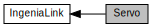
\includegraphics[width=224pt]{group__IL__SERVO}
\end{center}
\end{figure}
\subsection*{Data Structures}
\begin{DoxyCompactItemize}
\item 
struct \hyperlink{structil__servo__info__t}{il\+\_\+servo\+\_\+info\+\_\+t}
\begin{DoxyCompactList}\small\item\em Ingenia\+Link servo information. \end{DoxyCompactList}\end{DoxyCompactItemize}
\subsection*{Macros}
\begin{DoxyCompactItemize}
\item 
\#define \hyperlink{group__IL__SERVO_ga6c36d0853cb9bd4c71cee037421ec09a}{I\+L\+\_\+\+S\+E\+R\+V\+O\+\_\+\+S\+P\+\_\+\+T\+I\+M\+E\+O\+U\+T\+\_\+\+D\+EF}~1000
\begin{DoxyCompactList}\small\item\em Set-\/point acknowledge default timeout (ms). \end{DoxyCompactList}\item 
\#define \hyperlink{group__IL__SERVO_ga0a684ea427841d8ba4cf87b2d9a94d97}{I\+L\+\_\+\+S\+E\+R\+V\+O\+\_\+\+N\+A\+M\+E\+\_\+\+SZ}~9
\begin{DoxyCompactList}\small\item\em Servo name size (includes null termination). \end{DoxyCompactList}\item 
\#define \hyperlink{group__IL__SERVO_gaec19ad2892772d99664f16c55b9bc43f}{I\+L\+\_\+\+S\+E\+R\+V\+O\+\_\+\+S\+W\+\_\+\+V\+E\+R\+S\+I\+O\+N\+\_\+\+SZ}~9
\begin{DoxyCompactList}\small\item\em Servo software version size. \end{DoxyCompactList}\item 
\#define \hyperlink{group__IL__SERVO_ga18d9729ab800ffdda8ec81d8146a7e3f}{I\+L\+\_\+\+S\+E\+R\+V\+O\+\_\+\+H\+W\+\_\+\+V\+A\+R\+I\+A\+N\+T\+\_\+\+SZ}~5
\begin{DoxyCompactList}\small\item\em Hardware variant size. \end{DoxyCompactList}\item 
\#define \hyperlink{group__IL__SERVO_gaae195bbc7fd4c1d34122370e373a2fad}{I\+L\+\_\+\+S\+E\+R\+V\+O\+\_\+\+F\+L\+A\+G\+\_\+\+T\+G\+T\+\_\+\+R\+E\+A\+C\+H\+ED}~0x01
\begin{DoxyCompactList}\small\item\em Flags\+: Target reached. \end{DoxyCompactList}\item 
\#define \hyperlink{group__IL__SERVO_gac35b4c54f16936ff70f4e974a79fa586}{I\+L\+\_\+\+S\+E\+R\+V\+O\+\_\+\+F\+L\+A\+G\+\_\+\+I\+L\+I\+M\+\_\+\+A\+C\+T\+I\+VE}~0x02
\begin{DoxyCompactList}\small\item\em Flags\+: Internal limit active. \end{DoxyCompactList}\item 
\#define \hyperlink{group__IL__SERVO_ga683ef09e3c3e8133cfe1332a067cb88a}{I\+L\+\_\+\+S\+E\+R\+V\+O\+\_\+\+F\+L\+A\+G\+\_\+\+H\+O\+M\+I\+N\+G\+\_\+\+A\+TT}~0x04
\begin{DoxyCompactList}\small\item\em Flags\+: (Homing)\+: attained. \end{DoxyCompactList}\item 
\#define \hyperlink{group__IL__SERVO_gaa8b47a602774d828155efbc452bfbe66}{I\+L\+\_\+\+S\+E\+R\+V\+O\+\_\+\+F\+L\+A\+G\+\_\+\+H\+O\+M\+I\+N\+G\+\_\+\+E\+RR}~0x08
\begin{DoxyCompactList}\small\item\em Flags\+: (Homing)\+: error. \end{DoxyCompactList}\item 
\#define \hyperlink{group__IL__SERVO_gafa091abecc943d2133cd2a11bf1e6581}{I\+L\+\_\+\+S\+E\+R\+V\+O\+\_\+\+F\+L\+A\+G\+\_\+\+P\+V\+\_\+\+V\+Z\+E\+RO}~0x04
\begin{DoxyCompactList}\small\item\em Flags\+: (PV)\+: Vocity speed is zero. \end{DoxyCompactList}\item 
\#define \hyperlink{group__IL__SERVO_ga41e25c02b8b67f9d845f970cd6870144}{I\+L\+\_\+\+S\+E\+R\+V\+O\+\_\+\+F\+L\+A\+G\+\_\+\+P\+P\+\_\+\+S\+P\+A\+CK}~0x04
\begin{DoxyCompactList}\small\item\em Flags\+: (PP)\+: SP acknowledge. \end{DoxyCompactList}\item 
\#define \hyperlink{group__IL__SERVO_ga13208d747f34c53249e4e806dc1e88b9}{I\+L\+\_\+\+S\+E\+R\+V\+O\+\_\+\+F\+L\+A\+G\+\_\+\+I\+P\+\_\+\+A\+C\+T\+I\+VE}~0x04
\begin{DoxyCompactList}\small\item\em Flags\+: (IP)\+: active. \end{DoxyCompactList}\item 
\#define \hyperlink{group__IL__SERVO_gad862ccc1fcb5ee2969898185b2e8e10c}{I\+L\+\_\+\+S\+E\+R\+V\+O\+\_\+\+F\+L\+A\+G\+\_\+\+C\+S\+\_\+\+F\+O\+L\+L\+O\+WS}~0x04
\begin{DoxyCompactList}\small\item\em Flags\+: (C\+S\+T/\+C\+S\+V/\+C\+SP)\+: follow command value. \end{DoxyCompactList}\item 
\#define \hyperlink{group__IL__SERVO_gaa782f00113ceb5b0582471b8fe86a628}{I\+L\+\_\+\+S\+E\+R\+V\+O\+\_\+\+F\+L\+A\+G\+\_\+\+F\+E\+RR}~0x08
\begin{DoxyCompactList}\small\item\em Flags\+: (C\+S\+T/\+C\+S\+V/\+C\+S\+P/\+PV)\+: following error. \end{DoxyCompactList}\item 
\#define \hyperlink{group__IL__SERVO_gab8b5ab2cb8696d4781296b15ed4e0b67}{I\+L\+\_\+\+S\+E\+R\+V\+O\+\_\+\+F\+L\+A\+G\+\_\+\+I\+A\+N\+G\+L\+E\+\_\+\+D\+ET}~0x10
\begin{DoxyCompactList}\small\item\em Flags\+: Initial angle determination finished. \end{DoxyCompactList}\end{DoxyCompactItemize}
\subsection*{Typedefs}
\begin{DoxyCompactItemize}
\item 
typedef struct il\+\_\+servo \hyperlink{group__IL__SERVO_ga3369ddfcc33492fe3a28f96cf455b13e}{il\+\_\+servo\+\_\+t}
\begin{DoxyCompactList}\small\item\em Ingenia\+Link servo instance. \end{DoxyCompactList}\item 
typedef void($\ast$ \hyperlink{group__IL__SERVO_gad86cbd352b4ca4f73aa5bddece082a11}{il\+\_\+servo\+\_\+emcy\+\_\+subscriber\+\_\+cb\+\_\+t}) (void $\ast$ctx, uint32\+\_\+t code)
\begin{DoxyCompactList}\small\item\em Emergency subscriber callback. \end{DoxyCompactList}\item 
typedef void($\ast$ \hyperlink{group__IL__SERVO_ga60c0557ef5bc4c9e1b3bd32ea8d82861}{il\+\_\+servo\+\_\+state\+\_\+subscriber\+\_\+cb\+\_\+t}) (void $\ast$ctx, \hyperlink{group__IL__SERVO_ga34dfa4c089ba4ee833652ac6c40acd0d}{il\+\_\+servo\+\_\+state\+\_\+t} state, int flags)
\begin{DoxyCompactList}\small\item\em State updates subcriber callback. \end{DoxyCompactList}\end{DoxyCompactItemize}
\subsection*{Enumerations}
\begin{DoxyCompactItemize}
\item 
enum \hyperlink{group__IL__SERVO_ga34dfa4c089ba4ee833652ac6c40acd0d}{il\+\_\+servo\+\_\+state\+\_\+t} \{ \\*
\hyperlink{group__IL__SERVO_gga34dfa4c089ba4ee833652ac6c40acd0daa55953b65ace09c3bed52d4114840f1b}{I\+L\+\_\+\+S\+E\+R\+V\+O\+\_\+\+S\+T\+A\+T\+E\+\_\+\+N\+R\+DY}, 
\hyperlink{group__IL__SERVO_gga34dfa4c089ba4ee833652ac6c40acd0da23788d6ca281a3fbfed7562d75667adb}{I\+L\+\_\+\+S\+E\+R\+V\+O\+\_\+\+S\+T\+A\+T\+E\+\_\+\+D\+I\+S\+A\+B\+L\+ED}, 
\hyperlink{group__IL__SERVO_gga34dfa4c089ba4ee833652ac6c40acd0da526abc40393aee63a777f94b1a50f111}{I\+L\+\_\+\+S\+E\+R\+V\+O\+\_\+\+S\+T\+A\+T\+E\+\_\+\+R\+DY}, 
\hyperlink{group__IL__SERVO_gga34dfa4c089ba4ee833652ac6c40acd0da7cb1afaed87d34d110581a9e89509fdf}{I\+L\+\_\+\+S\+E\+R\+V\+O\+\_\+\+S\+T\+A\+T\+E\+\_\+\+ON}, 
\\*
\hyperlink{group__IL__SERVO_gga34dfa4c089ba4ee833652ac6c40acd0dab2f6b57025214e40be9fc2e1d69de2a5}{I\+L\+\_\+\+S\+E\+R\+V\+O\+\_\+\+S\+T\+A\+T\+E\+\_\+\+E\+N\+A\+B\+L\+ED}, 
\hyperlink{group__IL__SERVO_gga34dfa4c089ba4ee833652ac6c40acd0da3710762734b06272b18529e200585583}{I\+L\+\_\+\+S\+E\+R\+V\+O\+\_\+\+S\+T\+A\+T\+E\+\_\+\+Q\+S\+T\+OP}, 
\hyperlink{group__IL__SERVO_gga34dfa4c089ba4ee833652ac6c40acd0daf1d3fe0fefb6aecadacee5fb599375c0}{I\+L\+\_\+\+S\+E\+R\+V\+O\+\_\+\+S\+T\+A\+T\+E\+\_\+\+F\+A\+U\+L\+TR}, 
\hyperlink{group__IL__SERVO_gga34dfa4c089ba4ee833652ac6c40acd0da0e2beb3184098ba502e34354910f63f2}{I\+L\+\_\+\+S\+E\+R\+V\+O\+\_\+\+S\+T\+A\+T\+E\+\_\+\+F\+A\+U\+LT}
 \}\begin{DoxyCompactList}\small\item\em Servo states (equivalent to CiA 402 P\+DS states). \end{DoxyCompactList}
\item 
enum \hyperlink{group__IL__SERVO_ga6b3323798a8f235c225cc1d0cd27840a}{il\+\_\+servo\+\_\+mode\+\_\+t} \{ \\*
\hyperlink{group__IL__SERVO_gga6b3323798a8f235c225cc1d0cd27840aad8133deaaf79c917b29d388cf921a651}{I\+L\+\_\+\+S\+E\+R\+V\+O\+\_\+\+M\+O\+D\+E\+\_\+\+O\+LV}, 
\hyperlink{group__IL__SERVO_gga6b3323798a8f235c225cc1d0cd27840aaf49b82b9a802bb2b87cca3c777e8a72c}{I\+L\+\_\+\+S\+E\+R\+V\+O\+\_\+\+M\+O\+D\+E\+\_\+\+O\+LS}, 
\hyperlink{group__IL__SERVO_gga6b3323798a8f235c225cc1d0cd27840aa84502500bb9e2800c8c3bad60f30afd0}{I\+L\+\_\+\+S\+E\+R\+V\+O\+\_\+\+M\+O\+D\+E\+\_\+\+PP}, 
\hyperlink{group__IL__SERVO_gga6b3323798a8f235c225cc1d0cd27840aac670ce9cc12333e0d8b89e7e63db0f89}{I\+L\+\_\+\+S\+E\+R\+V\+O\+\_\+\+M\+O\+D\+E\+\_\+\+V\+EL}, 
\\*
\hyperlink{group__IL__SERVO_gga6b3323798a8f235c225cc1d0cd27840aa06f037b862ba17dfaac425ab706acf95}{I\+L\+\_\+\+S\+E\+R\+V\+O\+\_\+\+M\+O\+D\+E\+\_\+\+PV}, 
\hyperlink{group__IL__SERVO_gga6b3323798a8f235c225cc1d0cd27840aaf8243c2a154a13c399e9d5631593ce46}{I\+L\+\_\+\+S\+E\+R\+V\+O\+\_\+\+M\+O\+D\+E\+\_\+\+PT}, 
\hyperlink{group__IL__SERVO_gga6b3323798a8f235c225cc1d0cd27840aaf9aac6909e0810beac63271839113826}{I\+L\+\_\+\+S\+E\+R\+V\+O\+\_\+\+M\+O\+D\+E\+\_\+\+H\+O\+M\+I\+NG}, 
\hyperlink{group__IL__SERVO_gga6b3323798a8f235c225cc1d0cd27840aabc5de579ff40d7907da075bd60ef21fe}{I\+L\+\_\+\+S\+E\+R\+V\+O\+\_\+\+M\+O\+D\+E\+\_\+\+IP}, 
\\*
\hyperlink{group__IL__SERVO_gga6b3323798a8f235c225cc1d0cd27840aa4d36b5943ed7ab1d82483b310edae793}{I\+L\+\_\+\+S\+E\+R\+V\+O\+\_\+\+M\+O\+D\+E\+\_\+\+C\+SP}, 
\hyperlink{group__IL__SERVO_gga6b3323798a8f235c225cc1d0cd27840aa31597c98bdff233ab9dd1e1a9a238a3d}{I\+L\+\_\+\+S\+E\+R\+V\+O\+\_\+\+M\+O\+D\+E\+\_\+\+C\+SV}, 
\hyperlink{group__IL__SERVO_gga6b3323798a8f235c225cc1d0cd27840aadd4e3ef7edae53f0318cdebd41a00c9e}{I\+L\+\_\+\+S\+E\+R\+V\+O\+\_\+\+M\+O\+D\+E\+\_\+\+C\+ST}
 \}\begin{DoxyCompactList}\small\item\em Servo operation modes. \end{DoxyCompactList}
\item 
enum \hyperlink{group__IL__SERVO_ga4fb6d5223f5364f40c8f5c8018a00124}{il\+\_\+units\+\_\+torque\+\_\+t} \{ \hyperlink{group__IL__SERVO_gga4fb6d5223f5364f40c8f5c8018a00124a71f0c47645aba7c025c07a3793308518}{I\+L\+\_\+\+U\+N\+I\+T\+S\+\_\+\+T\+O\+R\+Q\+U\+E\+\_\+\+N\+A\+T\+I\+VE}, 
\hyperlink{group__IL__SERVO_gga4fb6d5223f5364f40c8f5c8018a00124a1caf6439156aabc869a67bea25f763fb}{I\+L\+\_\+\+U\+N\+I\+T\+S\+\_\+\+T\+O\+R\+Q\+U\+E\+\_\+\+M\+NM}, 
\hyperlink{group__IL__SERVO_gga4fb6d5223f5364f40c8f5c8018a00124a4a90e995ce79534d786c11dac9313a27}{I\+L\+\_\+\+U\+N\+I\+T\+S\+\_\+\+T\+O\+R\+Q\+U\+E\+\_\+\+NM}
 \}\begin{DoxyCompactList}\small\item\em Torque units. \end{DoxyCompactList}
\item 
enum \hyperlink{group__IL__SERVO_gaefeeab7931ae00097627941a79950799}{il\+\_\+units\+\_\+pos\+\_\+t} \{ \\*
\hyperlink{group__IL__SERVO_ggaefeeab7931ae00097627941a79950799afd38e43a05097d89890d0a35ae80a358}{I\+L\+\_\+\+U\+N\+I\+T\+S\+\_\+\+P\+O\+S\+\_\+\+N\+A\+T\+I\+VE}, 
\hyperlink{group__IL__SERVO_ggaefeeab7931ae00097627941a79950799a7dc0b4f7d0f9c2798c5ea5f1d04a4a8e}{I\+L\+\_\+\+U\+N\+I\+T\+S\+\_\+\+P\+O\+S\+\_\+\+R\+EV}, 
\hyperlink{group__IL__SERVO_ggaefeeab7931ae00097627941a79950799a44823ab17da1a86475c6dc3c9e85fa21}{I\+L\+\_\+\+U\+N\+I\+T\+S\+\_\+\+P\+O\+S\+\_\+\+R\+AD}, 
\hyperlink{group__IL__SERVO_ggaefeeab7931ae00097627941a79950799ad5a21928f5565c58ec6631ef735a73d4}{I\+L\+\_\+\+U\+N\+I\+T\+S\+\_\+\+P\+O\+S\+\_\+\+D\+EG}, 
\\*
\hyperlink{group__IL__SERVO_ggaefeeab7931ae00097627941a79950799a7b579b4273215a053d229a696e7a6b8a}{I\+L\+\_\+\+U\+N\+I\+T\+S\+\_\+\+P\+O\+S\+\_\+\+UM}, 
\hyperlink{group__IL__SERVO_ggaefeeab7931ae00097627941a79950799acf3bb2d9c0c753cf8f284322d653c5f2}{I\+L\+\_\+\+U\+N\+I\+T\+S\+\_\+\+P\+O\+S\+\_\+\+MM}, 
\hyperlink{group__IL__SERVO_ggaefeeab7931ae00097627941a79950799af95dfbcc88b47ade30d5211dc6dee09e}{I\+L\+\_\+\+U\+N\+I\+T\+S\+\_\+\+P\+O\+S\+\_\+M}
 \}\begin{DoxyCompactList}\small\item\em Position units. \end{DoxyCompactList}
\item 
enum \hyperlink{group__IL__SERVO_ga548eebb728eb841e157b57f2063203ee}{il\+\_\+units\+\_\+vel\+\_\+t} \{ \\*
\hyperlink{group__IL__SERVO_gga548eebb728eb841e157b57f2063203eea31f1d954a42ad41c75135c52483dc0fd}{I\+L\+\_\+\+U\+N\+I\+T\+S\+\_\+\+V\+E\+L\+\_\+\+N\+A\+T\+I\+VE}, 
\hyperlink{group__IL__SERVO_gga548eebb728eb841e157b57f2063203eea7ddfb276f1013c053617d2c5693af2a6}{I\+L\+\_\+\+U\+N\+I\+T\+S\+\_\+\+V\+E\+L\+\_\+\+R\+PS}, 
\hyperlink{group__IL__SERVO_gga548eebb728eb841e157b57f2063203eea945ffbca76bb3c0a21df0f242d24e18f}{I\+L\+\_\+\+U\+N\+I\+T\+S\+\_\+\+V\+E\+L\+\_\+\+R\+PM}, 
\hyperlink{group__IL__SERVO_gga548eebb728eb841e157b57f2063203eea7190dcc107d465da9e2ed577bc8d8ceb}{I\+L\+\_\+\+U\+N\+I\+T\+S\+\_\+\+V\+E\+L\+\_\+\+R\+A\+D\+\_\+S}, 
\\*
\hyperlink{group__IL__SERVO_gga548eebb728eb841e157b57f2063203eeaefca3b85d079add8af939073f1c4a2ba}{I\+L\+\_\+\+U\+N\+I\+T\+S\+\_\+\+V\+E\+L\+\_\+\+D\+E\+G\+\_\+S}, 
\hyperlink{group__IL__SERVO_gga548eebb728eb841e157b57f2063203eea792e330590bc7e221d6ee25bda627b7b}{I\+L\+\_\+\+U\+N\+I\+T\+S\+\_\+\+V\+E\+L\+\_\+\+U\+M\+\_\+S}, 
\hyperlink{group__IL__SERVO_gga548eebb728eb841e157b57f2063203eeacf5c8357769c71a6e6ff05e9cea1da35}{I\+L\+\_\+\+U\+N\+I\+T\+S\+\_\+\+V\+E\+L\+\_\+\+M\+M\+\_\+S}, 
\hyperlink{group__IL__SERVO_gga548eebb728eb841e157b57f2063203eea61616522994f03fef6dd301affee83ba}{I\+L\+\_\+\+U\+N\+I\+T\+S\+\_\+\+V\+E\+L\+\_\+\+M\+\_\+S}
 \}\begin{DoxyCompactList}\small\item\em Velocity units. \end{DoxyCompactList}
\item 
enum \hyperlink{group__IL__SERVO_ga07f4e0f292d1d7b5a6f1fc5c35fc151f}{il\+\_\+units\+\_\+acc\+\_\+t} \{ \\*
\hyperlink{group__IL__SERVO_gga07f4e0f292d1d7b5a6f1fc5c35fc151fa2dbb4edbf87bf40d1bec4e6b819570e5}{I\+L\+\_\+\+U\+N\+I\+T\+S\+\_\+\+A\+C\+C\+\_\+\+N\+A\+T\+I\+VE}, 
\hyperlink{group__IL__SERVO_gga07f4e0f292d1d7b5a6f1fc5c35fc151fa8fef1361fab6dab1481859efbb3b1c48}{I\+L\+\_\+\+U\+N\+I\+T\+S\+\_\+\+A\+C\+C\+\_\+\+R\+E\+V\+\_\+\+S2}, 
\hyperlink{group__IL__SERVO_gga07f4e0f292d1d7b5a6f1fc5c35fc151fadb4738643811868f758c9297c1199c70}{I\+L\+\_\+\+U\+N\+I\+T\+S\+\_\+\+A\+C\+C\+\_\+\+R\+A\+D\+\_\+\+S2}, 
\hyperlink{group__IL__SERVO_gga07f4e0f292d1d7b5a6f1fc5c35fc151fa9140fe3bc3c29c442a2af102f43abb77}{I\+L\+\_\+\+U\+N\+I\+T\+S\+\_\+\+A\+C\+C\+\_\+\+D\+E\+G\+\_\+\+S2}, 
\\*
\hyperlink{group__IL__SERVO_gga07f4e0f292d1d7b5a6f1fc5c35fc151fab6ee667f66aaae98136b1bae969467f7}{I\+L\+\_\+\+U\+N\+I\+T\+S\+\_\+\+A\+C\+C\+\_\+\+U\+M\+\_\+\+S2}, 
\hyperlink{group__IL__SERVO_gga07f4e0f292d1d7b5a6f1fc5c35fc151fa1cf13cf16f774312a603493c2e9961e4}{I\+L\+\_\+\+U\+N\+I\+T\+S\+\_\+\+A\+C\+C\+\_\+\+M\+M\+\_\+\+S2}, 
\hyperlink{group__IL__SERVO_gga07f4e0f292d1d7b5a6f1fc5c35fc151fa4de34cd9765e5671b419237519d33ec9}{I\+L\+\_\+\+U\+N\+I\+T\+S\+\_\+\+A\+C\+C\+\_\+\+M\+\_\+\+S2}
 \}\begin{DoxyCompactList}\small\item\em Acceleration units. \end{DoxyCompactList}
\end{DoxyCompactItemize}
\subsection*{Functions}
\begin{DoxyCompactItemize}
\item 
\hyperlink{common_8h_a6bb629d26c52bfe10519ba3176853f47}{I\+L\+\_\+\+E\+X\+P\+O\+RT} \hyperlink{group__IL__SERVO_ga3369ddfcc33492fe3a28f96cf455b13e}{il\+\_\+servo\+\_\+t} $\ast$ \hyperlink{group__IL__SERVO_gaa3728b10386d3b9f67258a95cb3c2913}{il\+\_\+servo\+\_\+create} (\hyperlink{group__IL__NET_ga0657204ab779a5b7a504aa0b895d1ae6}{il\+\_\+net\+\_\+t} $\ast$net, uint16\+\_\+t id, const char $\ast$dict)
\begin{DoxyCompactList}\small\item\em Create Ingenia\+Link servo instance. \end{DoxyCompactList}\item 
\hyperlink{common_8h_a6bb629d26c52bfe10519ba3176853f47}{I\+L\+\_\+\+E\+X\+P\+O\+RT} void \hyperlink{group__IL__SERVO_gade6d6e8ae2488af2a6ae6a6c484eaf32}{il\+\_\+servo\+\_\+destroy} (\hyperlink{group__IL__SERVO_ga3369ddfcc33492fe3a28f96cf455b13e}{il\+\_\+servo\+\_\+t} $\ast$servo)
\begin{DoxyCompactList}\small\item\em Destroy an Ingenia\+Link servo instance. \end{DoxyCompactList}\item 
\hyperlink{common_8h_a6bb629d26c52bfe10519ba3176853f47}{I\+L\+\_\+\+E\+X\+P\+O\+RT} int \hyperlink{group__IL__SERVO_ga1d0ef8479c2144e2abd9f18d7a875a34}{il\+\_\+servo\+\_\+reset} (\hyperlink{group__IL__SERVO_ga3369ddfcc33492fe3a28f96cf455b13e}{il\+\_\+servo\+\_\+t} $\ast$servo)
\begin{DoxyCompactList}\small\item\em Reset servo. \end{DoxyCompactList}\item 
\hyperlink{common_8h_a6bb629d26c52bfe10519ba3176853f47}{I\+L\+\_\+\+E\+X\+P\+O\+RT} void \hyperlink{group__IL__SERVO_ga52d4dfa8d34a7cce329d997c8ee8c38a}{il\+\_\+servo\+\_\+state\+\_\+get} (\hyperlink{group__IL__SERVO_ga3369ddfcc33492fe3a28f96cf455b13e}{il\+\_\+servo\+\_\+t} $\ast$servo, \hyperlink{group__IL__SERVO_ga34dfa4c089ba4ee833652ac6c40acd0d}{il\+\_\+servo\+\_\+state\+\_\+t} $\ast$state, int $\ast$flags)
\begin{DoxyCompactList}\small\item\em Obtain current servo P\+DS state. \end{DoxyCompactList}\item 
\hyperlink{common_8h_a6bb629d26c52bfe10519ba3176853f47}{I\+L\+\_\+\+E\+X\+P\+O\+RT} int \hyperlink{group__IL__SERVO_gab48c5b7f3f359ab4ad358525e9f69d88}{il\+\_\+servo\+\_\+state\+\_\+subscribe} (\hyperlink{group__IL__SERVO_ga3369ddfcc33492fe3a28f96cf455b13e}{il\+\_\+servo\+\_\+t} $\ast$servo, \hyperlink{group__IL__SERVO_ga60c0557ef5bc4c9e1b3bd32ea8d82861}{il\+\_\+servo\+\_\+state\+\_\+subscriber\+\_\+cb\+\_\+t} cb, void $\ast$ctx)
\begin{DoxyCompactList}\small\item\em Subscribe to state changes (and operation flags). \end{DoxyCompactList}\item 
\hyperlink{common_8h_a6bb629d26c52bfe10519ba3176853f47}{I\+L\+\_\+\+E\+X\+P\+O\+RT} void \hyperlink{group__IL__SERVO_gab9badbee2d7c812fd70f36e54b33f102}{il\+\_\+servo\+\_\+state\+\_\+unsubscribe} (\hyperlink{group__IL__SERVO_ga3369ddfcc33492fe3a28f96cf455b13e}{il\+\_\+servo\+\_\+t} $\ast$servo, int slot)
\begin{DoxyCompactList}\small\item\em Unsubscribe from state changes. \end{DoxyCompactList}\item 
\hyperlink{common_8h_a6bb629d26c52bfe10519ba3176853f47}{I\+L\+\_\+\+E\+X\+P\+O\+RT} int \hyperlink{group__IL__SERVO_gad64153fedf0e2c82b88b545de2a1e134}{il\+\_\+servo\+\_\+emcy\+\_\+subscribe} (\hyperlink{group__IL__SERVO_ga3369ddfcc33492fe3a28f96cf455b13e}{il\+\_\+servo\+\_\+t} $\ast$servo, \hyperlink{group__IL__SERVO_gad86cbd352b4ca4f73aa5bddece082a11}{il\+\_\+servo\+\_\+emcy\+\_\+subscriber\+\_\+cb\+\_\+t} cb, void $\ast$ctx)
\begin{DoxyCompactList}\small\item\em Subscribe to emergency messages. \end{DoxyCompactList}\item 
\hyperlink{common_8h_a6bb629d26c52bfe10519ba3176853f47}{I\+L\+\_\+\+E\+X\+P\+O\+RT} void \hyperlink{group__IL__SERVO_ga2bfe5b7de979ba3a7339292afa7c0a3b}{il\+\_\+servo\+\_\+emcy\+\_\+unsubscribe} (\hyperlink{group__IL__SERVO_ga3369ddfcc33492fe3a28f96cf455b13e}{il\+\_\+servo\+\_\+t} $\ast$servo, int slot)
\begin{DoxyCompactList}\small\item\em Unubscribe from emergency messages. \end{DoxyCompactList}\item 
\hyperlink{common_8h_a6bb629d26c52bfe10519ba3176853f47}{I\+L\+\_\+\+E\+X\+P\+O\+RT} \hyperlink{group__IL__DICT_gac2cb8ba7974d8506df3017879572fc84}{il\+\_\+dict\+\_\+t} $\ast$ \hyperlink{group__IL__SERVO_ga396350b82f3aeef0950533871c2d1214}{il\+\_\+servo\+\_\+dict\+\_\+get} (\hyperlink{group__IL__SERVO_ga3369ddfcc33492fe3a28f96cf455b13e}{il\+\_\+servo\+\_\+t} $\ast$servo)
\begin{DoxyCompactList}\small\item\em Obtain servo dictionary. \end{DoxyCompactList}\item 
\hyperlink{common_8h_a6bb629d26c52bfe10519ba3176853f47}{I\+L\+\_\+\+E\+X\+P\+O\+RT} int \hyperlink{group__IL__SERVO_ga5598b379a48c330d7c76ffb109088403}{il\+\_\+servo\+\_\+dict\+\_\+load} (\hyperlink{group__IL__SERVO_ga3369ddfcc33492fe3a28f96cf455b13e}{il\+\_\+servo\+\_\+t} $\ast$servo, const char $\ast$dict)
\begin{DoxyCompactList}\small\item\em Load a dictionary to the servo. \end{DoxyCompactList}\item 
\hyperlink{common_8h_a6bb629d26c52bfe10519ba3176853f47}{I\+L\+\_\+\+E\+X\+P\+O\+RT} int \hyperlink{group__IL__SERVO_ga4154f5f19c2826449c4e01021a9fa061}{il\+\_\+servo\+\_\+name\+\_\+get} (\hyperlink{group__IL__SERVO_ga3369ddfcc33492fe3a28f96cf455b13e}{il\+\_\+servo\+\_\+t} $\ast$servo, char $\ast$name, size\+\_\+t sz)
\begin{DoxyCompactList}\small\item\em Obtain servo name. \end{DoxyCompactList}\item 
\hyperlink{common_8h_a6bb629d26c52bfe10519ba3176853f47}{I\+L\+\_\+\+E\+X\+P\+O\+RT} int \hyperlink{group__IL__SERVO_gadd8ffb5ac5efa38c62e2d480f4c90475}{il\+\_\+servo\+\_\+name\+\_\+set} (\hyperlink{group__IL__SERVO_ga3369ddfcc33492fe3a28f96cf455b13e}{il\+\_\+servo\+\_\+t} $\ast$servo, const char $\ast$name)
\begin{DoxyCompactList}\small\item\em Set servo name. \end{DoxyCompactList}\item 
\hyperlink{common_8h_a6bb629d26c52bfe10519ba3176853f47}{I\+L\+\_\+\+E\+X\+P\+O\+RT} int \hyperlink{group__IL__SERVO_gac10a7958e9f2c4ef31ba2df3d7b51168}{il\+\_\+servo\+\_\+info\+\_\+get} (\hyperlink{group__IL__SERVO_ga3369ddfcc33492fe3a28f96cf455b13e}{il\+\_\+servo\+\_\+t} $\ast$servo, \hyperlink{structil__servo__info__t}{il\+\_\+servo\+\_\+info\+\_\+t} $\ast$info)
\begin{DoxyCompactList}\small\item\em Obtain servo information. \end{DoxyCompactList}\item 
\hyperlink{common_8h_a6bb629d26c52bfe10519ba3176853f47}{I\+L\+\_\+\+E\+X\+P\+O\+RT} int \hyperlink{group__IL__SERVO_gab2f6c3652bfea0818a2087434c5d4f6b}{il\+\_\+servo\+\_\+store\+\_\+all} (\hyperlink{group__IL__SERVO_ga3369ddfcc33492fe3a28f96cf455b13e}{il\+\_\+servo\+\_\+t} $\ast$servo)
\begin{DoxyCompactList}\small\item\em Store all servo current parameters to the N\+VM. \end{DoxyCompactList}\item 
\hyperlink{common_8h_a6bb629d26c52bfe10519ba3176853f47}{I\+L\+\_\+\+E\+X\+P\+O\+RT} int \hyperlink{group__IL__SERVO_ga665618a8278570eb3e1f35eecaa38048}{il\+\_\+servo\+\_\+store\+\_\+comm} (\hyperlink{group__IL__SERVO_ga3369ddfcc33492fe3a28f96cf455b13e}{il\+\_\+servo\+\_\+t} $\ast$servo)
\begin{DoxyCompactList}\small\item\em Store all servo current communications parameters to the N\+VM. \end{DoxyCompactList}\item 
\hyperlink{common_8h_a6bb629d26c52bfe10519ba3176853f47}{I\+L\+\_\+\+E\+X\+P\+O\+RT} int \hyperlink{group__IL__SERVO_gaaf4d6d6a1d9f90feaf7783a4a8bb5042}{il\+\_\+servo\+\_\+store\+\_\+app} (\hyperlink{group__IL__SERVO_ga3369ddfcc33492fe3a28f96cf455b13e}{il\+\_\+servo\+\_\+t} $\ast$servo)
\begin{DoxyCompactList}\small\item\em Store all servo current application parameters to the N\+VM. \end{DoxyCompactList}\item 
\hyperlink{common_8h_a6bb629d26c52bfe10519ba3176853f47}{I\+L\+\_\+\+E\+X\+P\+O\+RT} int \hyperlink{group__IL__SERVO_ga8bdb970bbe4c05d2b3f1d78268789bb3}{il\+\_\+servo\+\_\+units\+\_\+update} (\hyperlink{group__IL__SERVO_ga3369ddfcc33492fe3a28f96cf455b13e}{il\+\_\+servo\+\_\+t} $\ast$servo)
\begin{DoxyCompactList}\small\item\em Update units scaling factors. \end{DoxyCompactList}\item 
\hyperlink{common_8h_a6bb629d26c52bfe10519ba3176853f47}{I\+L\+\_\+\+E\+X\+P\+O\+RT} double \hyperlink{group__IL__SERVO_gacde3271e378552034d8c0966ead4f941}{il\+\_\+servo\+\_\+units\+\_\+factor} (\hyperlink{group__IL__SERVO_ga3369ddfcc33492fe3a28f96cf455b13e}{il\+\_\+servo\+\_\+t} $\ast$servo, const \hyperlink{structil__reg__t}{il\+\_\+reg\+\_\+t} $\ast$reg)
\begin{DoxyCompactList}\small\item\em Obtain the units scale factor associated with the given register. \end{DoxyCompactList}\item 
\hyperlink{common_8h_a6bb629d26c52bfe10519ba3176853f47}{I\+L\+\_\+\+E\+X\+P\+O\+RT} \hyperlink{group__IL__SERVO_ga4fb6d5223f5364f40c8f5c8018a00124}{il\+\_\+units\+\_\+torque\+\_\+t} \hyperlink{group__IL__SERVO_gaf227fedcfd9602135cefd6bf240202c6}{il\+\_\+servo\+\_\+units\+\_\+torque\+\_\+get} (\hyperlink{group__IL__SERVO_ga3369ddfcc33492fe3a28f96cf455b13e}{il\+\_\+servo\+\_\+t} $\ast$servo)
\begin{DoxyCompactList}\small\item\em Get the torque units. \end{DoxyCompactList}\item 
\hyperlink{common_8h_a6bb629d26c52bfe10519ba3176853f47}{I\+L\+\_\+\+E\+X\+P\+O\+RT} void \hyperlink{group__IL__SERVO_gab5d0b378b678e0fd6d1a571eb90ab66f}{il\+\_\+servo\+\_\+units\+\_\+torque\+\_\+set} (\hyperlink{group__IL__SERVO_ga3369ddfcc33492fe3a28f96cf455b13e}{il\+\_\+servo\+\_\+t} $\ast$servo, \hyperlink{group__IL__SERVO_ga4fb6d5223f5364f40c8f5c8018a00124}{il\+\_\+units\+\_\+torque\+\_\+t} units)
\begin{DoxyCompactList}\small\item\em Set the torque units. \end{DoxyCompactList}\item 
\hyperlink{common_8h_a6bb629d26c52bfe10519ba3176853f47}{I\+L\+\_\+\+E\+X\+P\+O\+RT} \hyperlink{group__IL__SERVO_gaefeeab7931ae00097627941a79950799}{il\+\_\+units\+\_\+pos\+\_\+t} \hyperlink{group__IL__SERVO_gad561c34b2b3d7646e8cc9cb360e2f87e}{il\+\_\+servo\+\_\+units\+\_\+pos\+\_\+get} (\hyperlink{group__IL__SERVO_ga3369ddfcc33492fe3a28f96cf455b13e}{il\+\_\+servo\+\_\+t} $\ast$servo)
\begin{DoxyCompactList}\small\item\em Get the position units. \end{DoxyCompactList}\item 
\hyperlink{common_8h_a6bb629d26c52bfe10519ba3176853f47}{I\+L\+\_\+\+E\+X\+P\+O\+RT} void \hyperlink{group__IL__SERVO_ga1a64e31ed42e99bff4a577fc8b2ad076}{il\+\_\+servo\+\_\+units\+\_\+pos\+\_\+set} (\hyperlink{group__IL__SERVO_ga3369ddfcc33492fe3a28f96cf455b13e}{il\+\_\+servo\+\_\+t} $\ast$servo, \hyperlink{group__IL__SERVO_gaefeeab7931ae00097627941a79950799}{il\+\_\+units\+\_\+pos\+\_\+t} units)
\begin{DoxyCompactList}\small\item\em Set the position units. \end{DoxyCompactList}\item 
\hyperlink{common_8h_a6bb629d26c52bfe10519ba3176853f47}{I\+L\+\_\+\+E\+X\+P\+O\+RT} \hyperlink{group__IL__SERVO_ga548eebb728eb841e157b57f2063203ee}{il\+\_\+units\+\_\+vel\+\_\+t} \hyperlink{group__IL__SERVO_gaeb7615b200f236722ef98bf1b8b594c2}{il\+\_\+servo\+\_\+units\+\_\+vel\+\_\+get} (\hyperlink{group__IL__SERVO_ga3369ddfcc33492fe3a28f96cf455b13e}{il\+\_\+servo\+\_\+t} $\ast$servo)
\begin{DoxyCompactList}\small\item\em Get the velocity units. \end{DoxyCompactList}\item 
\hyperlink{common_8h_a6bb629d26c52bfe10519ba3176853f47}{I\+L\+\_\+\+E\+X\+P\+O\+RT} void \hyperlink{group__IL__SERVO_gacd15dfc7141865bcb63912888aad71ba}{il\+\_\+servo\+\_\+units\+\_\+vel\+\_\+set} (\hyperlink{group__IL__SERVO_ga3369ddfcc33492fe3a28f96cf455b13e}{il\+\_\+servo\+\_\+t} $\ast$servo, \hyperlink{group__IL__SERVO_ga548eebb728eb841e157b57f2063203ee}{il\+\_\+units\+\_\+vel\+\_\+t} units)
\begin{DoxyCompactList}\small\item\em Set the velocity units. \end{DoxyCompactList}\item 
\hyperlink{common_8h_a6bb629d26c52bfe10519ba3176853f47}{I\+L\+\_\+\+E\+X\+P\+O\+RT} \hyperlink{group__IL__SERVO_ga07f4e0f292d1d7b5a6f1fc5c35fc151f}{il\+\_\+units\+\_\+acc\+\_\+t} \hyperlink{group__IL__SERVO_ga312b0ca5ea200c5ec1c60adad84017a2}{il\+\_\+servo\+\_\+units\+\_\+acc\+\_\+get} (\hyperlink{group__IL__SERVO_ga3369ddfcc33492fe3a28f96cf455b13e}{il\+\_\+servo\+\_\+t} $\ast$servo)
\begin{DoxyCompactList}\small\item\em Get the acceleration units. \end{DoxyCompactList}\item 
\hyperlink{common_8h_a6bb629d26c52bfe10519ba3176853f47}{I\+L\+\_\+\+E\+X\+P\+O\+RT} void \hyperlink{group__IL__SERVO_gae06520e0e95dc18d1586c6b76d303b80}{il\+\_\+servo\+\_\+units\+\_\+acc\+\_\+set} (\hyperlink{group__IL__SERVO_ga3369ddfcc33492fe3a28f96cf455b13e}{il\+\_\+servo\+\_\+t} $\ast$servo, \hyperlink{group__IL__SERVO_ga07f4e0f292d1d7b5a6f1fc5c35fc151f}{il\+\_\+units\+\_\+acc\+\_\+t} units)
\begin{DoxyCompactList}\small\item\em Set the acceleration units. \end{DoxyCompactList}\item 
\hyperlink{common_8h_a6bb629d26c52bfe10519ba3176853f47}{I\+L\+\_\+\+E\+X\+P\+O\+RT} int \hyperlink{group__IL__SERVO_ga8b1bd006fa9cd70b20097f723891122b}{il\+\_\+servo\+\_\+raw\+\_\+read\+\_\+u8} (\hyperlink{group__IL__SERVO_ga3369ddfcc33492fe3a28f96cf455b13e}{il\+\_\+servo\+\_\+t} $\ast$servo, const \hyperlink{structil__reg__t}{il\+\_\+reg\+\_\+t} $\ast$reg, const char $\ast$id, uint8\+\_\+t $\ast$buf)
\begin{DoxyCompactList}\small\item\em Read unsigned 8-\/bit value from a register. \end{DoxyCompactList}\item 
\hyperlink{common_8h_a6bb629d26c52bfe10519ba3176853f47}{I\+L\+\_\+\+E\+X\+P\+O\+RT} int \hyperlink{group__IL__SERVO_ga1d6b70bd773328b9cd7e63adcb5fdb24}{il\+\_\+servo\+\_\+raw\+\_\+read\+\_\+s8} (\hyperlink{group__IL__SERVO_ga3369ddfcc33492fe3a28f96cf455b13e}{il\+\_\+servo\+\_\+t} $\ast$servo, const \hyperlink{structil__reg__t}{il\+\_\+reg\+\_\+t} $\ast$reg, const char $\ast$id, int8\+\_\+t $\ast$buf)
\begin{DoxyCompactList}\small\item\em Read signed 8-\/bit value from a register. \end{DoxyCompactList}\item 
\hyperlink{common_8h_a6bb629d26c52bfe10519ba3176853f47}{I\+L\+\_\+\+E\+X\+P\+O\+RT} int \hyperlink{group__IL__SERVO_gae62ff2541783a740d8c2b623e489a703}{il\+\_\+servo\+\_\+raw\+\_\+read\+\_\+u16} (\hyperlink{group__IL__SERVO_ga3369ddfcc33492fe3a28f96cf455b13e}{il\+\_\+servo\+\_\+t} $\ast$servo, const \hyperlink{structil__reg__t}{il\+\_\+reg\+\_\+t} $\ast$reg, const char $\ast$id, uint16\+\_\+t $\ast$buf)
\begin{DoxyCompactList}\small\item\em Read unsigned 16-\/bit value from a register. \end{DoxyCompactList}\item 
\hyperlink{common_8h_a6bb629d26c52bfe10519ba3176853f47}{I\+L\+\_\+\+E\+X\+P\+O\+RT} int \hyperlink{group__IL__SERVO_ga9ac45aa67ec61b0dcbe2827a4484bfd5}{il\+\_\+servo\+\_\+raw\+\_\+read\+\_\+s16} (\hyperlink{group__IL__SERVO_ga3369ddfcc33492fe3a28f96cf455b13e}{il\+\_\+servo\+\_\+t} $\ast$servo, const \hyperlink{structil__reg__t}{il\+\_\+reg\+\_\+t} $\ast$reg, const char $\ast$id, int16\+\_\+t $\ast$buf)
\begin{DoxyCompactList}\small\item\em Read signed 16-\/bit value from a register. \end{DoxyCompactList}\item 
\hyperlink{common_8h_a6bb629d26c52bfe10519ba3176853f47}{I\+L\+\_\+\+E\+X\+P\+O\+RT} int \hyperlink{group__IL__SERVO_ga887a2e63754e1a4ebee5a0ab8310cc56}{il\+\_\+servo\+\_\+raw\+\_\+read\+\_\+u32} (\hyperlink{group__IL__SERVO_ga3369ddfcc33492fe3a28f96cf455b13e}{il\+\_\+servo\+\_\+t} $\ast$servo, const \hyperlink{structil__reg__t}{il\+\_\+reg\+\_\+t} $\ast$reg, const char $\ast$id, uint32\+\_\+t $\ast$buf)
\begin{DoxyCompactList}\small\item\em Read unsigned 32-\/bit value from a register. \end{DoxyCompactList}\item 
\hyperlink{common_8h_a6bb629d26c52bfe10519ba3176853f47}{I\+L\+\_\+\+E\+X\+P\+O\+RT} int \hyperlink{group__IL__SERVO_gab0c5bbb4fcd2784f10fab3648dc405c4}{il\+\_\+servo\+\_\+raw\+\_\+read\+\_\+s32} (\hyperlink{group__IL__SERVO_ga3369ddfcc33492fe3a28f96cf455b13e}{il\+\_\+servo\+\_\+t} $\ast$servo, const \hyperlink{structil__reg__t}{il\+\_\+reg\+\_\+t} $\ast$reg, const char $\ast$id, int32\+\_\+t $\ast$buf)
\begin{DoxyCompactList}\small\item\em Read signed 32-\/bit value from a register. \end{DoxyCompactList}\item 
\hyperlink{common_8h_a6bb629d26c52bfe10519ba3176853f47}{I\+L\+\_\+\+E\+X\+P\+O\+RT} int \hyperlink{group__IL__SERVO_ga254f9ed1043d3cc6e7175b0bb6a0c2c9}{il\+\_\+servo\+\_\+raw\+\_\+read\+\_\+u64} (\hyperlink{group__IL__SERVO_ga3369ddfcc33492fe3a28f96cf455b13e}{il\+\_\+servo\+\_\+t} $\ast$servo, const \hyperlink{structil__reg__t}{il\+\_\+reg\+\_\+t} $\ast$reg, const char $\ast$id, uint64\+\_\+t $\ast$buf)
\begin{DoxyCompactList}\small\item\em Read unsigned 64-\/bit value from a register. \end{DoxyCompactList}\item 
\hyperlink{common_8h_a6bb629d26c52bfe10519ba3176853f47}{I\+L\+\_\+\+E\+X\+P\+O\+RT} int \hyperlink{group__IL__SERVO_ga5caadeb6cb861b7a8b91dbb98113988f}{il\+\_\+servo\+\_\+raw\+\_\+read\+\_\+s64} (\hyperlink{group__IL__SERVO_ga3369ddfcc33492fe3a28f96cf455b13e}{il\+\_\+servo\+\_\+t} $\ast$servo, const \hyperlink{structil__reg__t}{il\+\_\+reg\+\_\+t} $\ast$reg, const char $\ast$id, int64\+\_\+t $\ast$buf)
\begin{DoxyCompactList}\small\item\em Read signed 64-\/bit value from a register. \end{DoxyCompactList}\item 
\hyperlink{common_8h_a6bb629d26c52bfe10519ba3176853f47}{I\+L\+\_\+\+E\+X\+P\+O\+RT} int \hyperlink{group__IL__SERVO_gacf0d6571be514e23c09581834203d90e}{il\+\_\+servo\+\_\+raw\+\_\+read\+\_\+float} (\hyperlink{group__IL__SERVO_ga3369ddfcc33492fe3a28f96cf455b13e}{il\+\_\+servo\+\_\+t} $\ast$servo, const \hyperlink{structil__reg__t}{il\+\_\+reg\+\_\+t} $\ast$reg, const char $\ast$id, float $\ast$buf)
\begin{DoxyCompactList}\small\item\em Read signed 64-\/bit value from a register. \end{DoxyCompactList}\item 
\hyperlink{common_8h_a6bb629d26c52bfe10519ba3176853f47}{I\+L\+\_\+\+E\+X\+P\+O\+RT} int \hyperlink{group__IL__SERVO_gad3b94f5a9811dd5a52bb306e92f92944}{il\+\_\+servo\+\_\+read} (\hyperlink{group__IL__SERVO_ga3369ddfcc33492fe3a28f96cf455b13e}{il\+\_\+servo\+\_\+t} $\ast$servo, const \hyperlink{structil__reg__t}{il\+\_\+reg\+\_\+t} $\ast$reg, const char $\ast$id, double $\ast$buf)
\begin{DoxyCompactList}\small\item\em Read a register. \end{DoxyCompactList}\item 
\hyperlink{common_8h_a6bb629d26c52bfe10519ba3176853f47}{I\+L\+\_\+\+E\+X\+P\+O\+RT} int \hyperlink{group__IL__SERVO_ga05c1c7c4d30c882744008de007686f3f}{il\+\_\+servo\+\_\+raw\+\_\+write\+\_\+u8} (\hyperlink{group__IL__SERVO_ga3369ddfcc33492fe3a28f96cf455b13e}{il\+\_\+servo\+\_\+t} $\ast$servo, const \hyperlink{structil__reg__t}{il\+\_\+reg\+\_\+t} $\ast$reg, const char $\ast$id, uint8\+\_\+t val, int confirm)
\begin{DoxyCompactList}\small\item\em Write unsigned 8-\/bit integer to a register. \end{DoxyCompactList}\item 
\hyperlink{common_8h_a6bb629d26c52bfe10519ba3176853f47}{I\+L\+\_\+\+E\+X\+P\+O\+RT} int \hyperlink{group__IL__SERVO_gafea21fc3b0adb4208a0571c87f979c50}{il\+\_\+servo\+\_\+raw\+\_\+write\+\_\+s8} (\hyperlink{group__IL__SERVO_ga3369ddfcc33492fe3a28f96cf455b13e}{il\+\_\+servo\+\_\+t} $\ast$servo, const \hyperlink{structil__reg__t}{il\+\_\+reg\+\_\+t} $\ast$reg, const char $\ast$id, int8\+\_\+t val, int confirm)
\begin{DoxyCompactList}\small\item\em Write signed 8-\/bit integer to a register. \end{DoxyCompactList}\item 
\hyperlink{common_8h_a6bb629d26c52bfe10519ba3176853f47}{I\+L\+\_\+\+E\+X\+P\+O\+RT} int \hyperlink{group__IL__SERVO_gae504512849138dc97ab7e5c51a1a6a02}{il\+\_\+servo\+\_\+raw\+\_\+write\+\_\+u16} (\hyperlink{group__IL__SERVO_ga3369ddfcc33492fe3a28f96cf455b13e}{il\+\_\+servo\+\_\+t} $\ast$servo, const \hyperlink{structil__reg__t}{il\+\_\+reg\+\_\+t} $\ast$reg, const char $\ast$id, uint16\+\_\+t val, int confirm)
\begin{DoxyCompactList}\small\item\em Write unsigned 16-\/bit integer to a register. \end{DoxyCompactList}\item 
\hyperlink{common_8h_a6bb629d26c52bfe10519ba3176853f47}{I\+L\+\_\+\+E\+X\+P\+O\+RT} int \hyperlink{group__IL__SERVO_ga42b17982936b1ce7982e5d16c3f6c090}{il\+\_\+servo\+\_\+raw\+\_\+write\+\_\+s16} (\hyperlink{group__IL__SERVO_ga3369ddfcc33492fe3a28f96cf455b13e}{il\+\_\+servo\+\_\+t} $\ast$servo, const \hyperlink{structil__reg__t}{il\+\_\+reg\+\_\+t} $\ast$reg, const char $\ast$id, int16\+\_\+t val, int confirm)
\begin{DoxyCompactList}\small\item\em Write signed 16-\/bit integer to a register. \end{DoxyCompactList}\item 
\hyperlink{common_8h_a6bb629d26c52bfe10519ba3176853f47}{I\+L\+\_\+\+E\+X\+P\+O\+RT} int \hyperlink{group__IL__SERVO_gac212376609f84669eb9792b676f453a3}{il\+\_\+servo\+\_\+raw\+\_\+write\+\_\+u32} (\hyperlink{group__IL__SERVO_ga3369ddfcc33492fe3a28f96cf455b13e}{il\+\_\+servo\+\_\+t} $\ast$servo, const \hyperlink{structil__reg__t}{il\+\_\+reg\+\_\+t} $\ast$reg, const char $\ast$id, uint32\+\_\+t val, int confirm)
\begin{DoxyCompactList}\small\item\em Write unsigned 32-\/bit integer to a register. \end{DoxyCompactList}\item 
\hyperlink{common_8h_a6bb629d26c52bfe10519ba3176853f47}{I\+L\+\_\+\+E\+X\+P\+O\+RT} int \hyperlink{group__IL__SERVO_gac07e7c8a81f9905d1fa9b447395270bc}{il\+\_\+servo\+\_\+raw\+\_\+write\+\_\+s32} (\hyperlink{group__IL__SERVO_ga3369ddfcc33492fe3a28f96cf455b13e}{il\+\_\+servo\+\_\+t} $\ast$servo, const \hyperlink{structil__reg__t}{il\+\_\+reg\+\_\+t} $\ast$reg, const char $\ast$id, int32\+\_\+t val, int confirm)
\begin{DoxyCompactList}\small\item\em Write signed 32-\/bit integer to a register. \end{DoxyCompactList}\item 
\hyperlink{common_8h_a6bb629d26c52bfe10519ba3176853f47}{I\+L\+\_\+\+E\+X\+P\+O\+RT} int \hyperlink{group__IL__SERVO_gacd041c7dd2ac1ec99d2cf1aa6f046a00}{il\+\_\+servo\+\_\+raw\+\_\+write\+\_\+u64} (\hyperlink{group__IL__SERVO_ga3369ddfcc33492fe3a28f96cf455b13e}{il\+\_\+servo\+\_\+t} $\ast$servo, const \hyperlink{structil__reg__t}{il\+\_\+reg\+\_\+t} $\ast$reg, const char $\ast$id, uint64\+\_\+t val, int confirm)
\begin{DoxyCompactList}\small\item\em Write unsigned 64-\/bit integer to a register. \end{DoxyCompactList}\item 
\hyperlink{common_8h_a6bb629d26c52bfe10519ba3176853f47}{I\+L\+\_\+\+E\+X\+P\+O\+RT} int \hyperlink{group__IL__SERVO_ga4ac4489c10367847a0d62d53ebf25a60}{il\+\_\+servo\+\_\+raw\+\_\+write\+\_\+s64} (\hyperlink{group__IL__SERVO_ga3369ddfcc33492fe3a28f96cf455b13e}{il\+\_\+servo\+\_\+t} $\ast$servo, const \hyperlink{structil__reg__t}{il\+\_\+reg\+\_\+t} $\ast$reg, const char $\ast$id, int64\+\_\+t val, int confirm)
\begin{DoxyCompactList}\small\item\em Write signed 64-\/bit integer to a register. \end{DoxyCompactList}\item 
\hyperlink{common_8h_a6bb629d26c52bfe10519ba3176853f47}{I\+L\+\_\+\+E\+X\+P\+O\+RT} int \hyperlink{group__IL__SERVO_ga56da0b13de04887cc5a6f9b2d4e7497e}{il\+\_\+servo\+\_\+raw\+\_\+write\+\_\+float} (\hyperlink{group__IL__SERVO_ga3369ddfcc33492fe3a28f96cf455b13e}{il\+\_\+servo\+\_\+t} $\ast$servo, const \hyperlink{structil__reg__t}{il\+\_\+reg\+\_\+t} $\ast$reg, const char $\ast$id, float val, int confirm)
\begin{DoxyCompactList}\small\item\em Write float to a register. \end{DoxyCompactList}\item 
\hyperlink{common_8h_a6bb629d26c52bfe10519ba3176853f47}{I\+L\+\_\+\+E\+X\+P\+O\+RT} int \hyperlink{group__IL__SERVO_gad1474e21342f4f02e6435d3f6d66dec1}{il\+\_\+servo\+\_\+write} (\hyperlink{group__IL__SERVO_ga3369ddfcc33492fe3a28f96cf455b13e}{il\+\_\+servo\+\_\+t} $\ast$servo, const \hyperlink{structil__reg__t}{il\+\_\+reg\+\_\+t} $\ast$reg, const char $\ast$id, double val, int confirm)
\begin{DoxyCompactList}\small\item\em Write to a register. \end{DoxyCompactList}\item 
\hyperlink{common_8h_a6bb629d26c52bfe10519ba3176853f47}{I\+L\+\_\+\+E\+X\+P\+O\+RT} int \hyperlink{group__IL__SERVO_ga8b5938454ac8183a514d11203f2e6197}{il\+\_\+servo\+\_\+disable} (\hyperlink{group__IL__SERVO_ga3369ddfcc33492fe3a28f96cf455b13e}{il\+\_\+servo\+\_\+t} $\ast$servo)
\begin{DoxyCompactList}\small\item\em Disable servo P\+DS. \end{DoxyCompactList}\item 
\hyperlink{common_8h_a6bb629d26c52bfe10519ba3176853f47}{I\+L\+\_\+\+E\+X\+P\+O\+RT} int \hyperlink{group__IL__SERVO_ga9ad6a595ca932caf31c2500de1e8a812}{il\+\_\+servo\+\_\+switch\+\_\+on} (\hyperlink{group__IL__SERVO_ga3369ddfcc33492fe3a28f96cf455b13e}{il\+\_\+servo\+\_\+t} $\ast$servo, int timeout)
\begin{DoxyCompactList}\small\item\em Switch on servo P\+DS. \end{DoxyCompactList}\item 
\hyperlink{common_8h_a6bb629d26c52bfe10519ba3176853f47}{I\+L\+\_\+\+E\+X\+P\+O\+RT} int \hyperlink{group__IL__SERVO_gaee57b72c5f6d4756a6a914edbf0db0d9}{il\+\_\+servo\+\_\+enable} (\hyperlink{group__IL__SERVO_ga3369ddfcc33492fe3a28f96cf455b13e}{il\+\_\+servo\+\_\+t} $\ast$servo, int timeout)
\begin{DoxyCompactList}\small\item\em Enable servo P\+DS. \end{DoxyCompactList}\item 
\hyperlink{common_8h_a6bb629d26c52bfe10519ba3176853f47}{I\+L\+\_\+\+E\+X\+P\+O\+RT} int \hyperlink{group__IL__SERVO_ga75fbdd6046af1825619d2710580911e2}{il\+\_\+servo\+\_\+fault\+\_\+reset} (\hyperlink{group__IL__SERVO_ga3369ddfcc33492fe3a28f96cf455b13e}{il\+\_\+servo\+\_\+t} $\ast$servo)
\begin{DoxyCompactList}\small\item\em Reset the drive fault state. \end{DoxyCompactList}\item 
\hyperlink{common_8h_a6bb629d26c52bfe10519ba3176853f47}{I\+L\+\_\+\+E\+X\+P\+O\+RT} int \hyperlink{group__IL__SERVO_ga7f545d6dd93e52f55688bb03ee263004}{il\+\_\+servo\+\_\+mode\+\_\+get} (\hyperlink{group__IL__SERVO_ga3369ddfcc33492fe3a28f96cf455b13e}{il\+\_\+servo\+\_\+t} $\ast$servo, \hyperlink{group__IL__SERVO_ga6b3323798a8f235c225cc1d0cd27840a}{il\+\_\+servo\+\_\+mode\+\_\+t} $\ast$mode)
\begin{DoxyCompactList}\small\item\em Get the servo operation mode. \end{DoxyCompactList}\item 
\hyperlink{common_8h_a6bb629d26c52bfe10519ba3176853f47}{I\+L\+\_\+\+E\+X\+P\+O\+RT} int \hyperlink{group__IL__SERVO_ga9ef9a84e8b6aa1ee23d301dbd93b8b2f}{il\+\_\+servo\+\_\+mode\+\_\+set} (\hyperlink{group__IL__SERVO_ga3369ddfcc33492fe3a28f96cf455b13e}{il\+\_\+servo\+\_\+t} $\ast$servo, \hyperlink{group__IL__SERVO_ga6b3323798a8f235c225cc1d0cd27840a}{il\+\_\+servo\+\_\+mode\+\_\+t} mode)
\begin{DoxyCompactList}\small\item\em Set the servo operation mode. \end{DoxyCompactList}\item 
\hyperlink{common_8h_a6bb629d26c52bfe10519ba3176853f47}{I\+L\+\_\+\+E\+X\+P\+O\+RT} int \hyperlink{group__IL__SERVO_ga245d1c9ecdbee76adff2b79757ebf158}{il\+\_\+servo\+\_\+ol\+\_\+voltage\+\_\+get} (\hyperlink{group__IL__SERVO_ga3369ddfcc33492fe3a28f96cf455b13e}{il\+\_\+servo\+\_\+t} $\ast$servo, double $\ast$voltage)
\begin{DoxyCompactList}\small\item\em Get the open loop voltage. \end{DoxyCompactList}\item 
\hyperlink{common_8h_a6bb629d26c52bfe10519ba3176853f47}{I\+L\+\_\+\+E\+X\+P\+O\+RT} int \hyperlink{group__IL__SERVO_ga3aec778ff294237e8e32a651ec8e215d}{il\+\_\+servo\+\_\+ol\+\_\+voltage\+\_\+set} (\hyperlink{group__IL__SERVO_ga3369ddfcc33492fe3a28f96cf455b13e}{il\+\_\+servo\+\_\+t} $\ast$servo, double voltage)
\begin{DoxyCompactList}\small\item\em Set the open loop voltage. \end{DoxyCompactList}\item 
\hyperlink{common_8h_a6bb629d26c52bfe10519ba3176853f47}{I\+L\+\_\+\+E\+X\+P\+O\+RT} int \hyperlink{group__IL__SERVO_ga190f42e03d0a1255efd92df375690f02}{il\+\_\+servo\+\_\+ol\+\_\+frequency\+\_\+get} (\hyperlink{group__IL__SERVO_ga3369ddfcc33492fe3a28f96cf455b13e}{il\+\_\+servo\+\_\+t} $\ast$servo, double $\ast$freq)
\begin{DoxyCompactList}\small\item\em Get the open loop frequency. \end{DoxyCompactList}\item 
\hyperlink{common_8h_a6bb629d26c52bfe10519ba3176853f47}{I\+L\+\_\+\+E\+X\+P\+O\+RT} int \hyperlink{group__IL__SERVO_ga7032da0b86cc1f6b139f10993c567b8a}{il\+\_\+servo\+\_\+ol\+\_\+frequency\+\_\+set} (\hyperlink{group__IL__SERVO_ga3369ddfcc33492fe3a28f96cf455b13e}{il\+\_\+servo\+\_\+t} $\ast$servo, double freq)
\begin{DoxyCompactList}\small\item\em Set the open loop frequency. \end{DoxyCompactList}\item 
\hyperlink{common_8h_a6bb629d26c52bfe10519ba3176853f47}{I\+L\+\_\+\+E\+X\+P\+O\+RT} int \hyperlink{group__IL__SERVO_gaf7cf26ed91ae60e5f049b056009783e0}{il\+\_\+servo\+\_\+homing\+\_\+start} (\hyperlink{group__IL__SERVO_ga3369ddfcc33492fe3a28f96cf455b13e}{il\+\_\+servo\+\_\+t} $\ast$servo)
\begin{DoxyCompactList}\small\item\em Start homing. \end{DoxyCompactList}\item 
\hyperlink{common_8h_a6bb629d26c52bfe10519ba3176853f47}{I\+L\+\_\+\+E\+X\+P\+O\+RT} int \hyperlink{group__IL__SERVO_gad55d208e57e674e0c1a31b995563e96d}{il\+\_\+servo\+\_\+homing\+\_\+wait} (\hyperlink{group__IL__SERVO_ga3369ddfcc33492fe3a28f96cf455b13e}{il\+\_\+servo\+\_\+t} $\ast$servo, int timeout)
\begin{DoxyCompactList}\small\item\em Wait until homing completes. \end{DoxyCompactList}\item 
\hyperlink{common_8h_a6bb629d26c52bfe10519ba3176853f47}{I\+L\+\_\+\+E\+X\+P\+O\+RT} int \hyperlink{group__IL__SERVO_ga77eb2ebb33ac5bc9e3eac7b3ae90e25b}{il\+\_\+servo\+\_\+torque\+\_\+get} (\hyperlink{group__IL__SERVO_ga3369ddfcc33492fe3a28f96cf455b13e}{il\+\_\+servo\+\_\+t} $\ast$servo, double $\ast$torque)
\begin{DoxyCompactList}\small\item\em Get the actual servo torque. \end{DoxyCompactList}\item 
\hyperlink{common_8h_a6bb629d26c52bfe10519ba3176853f47}{I\+L\+\_\+\+E\+X\+P\+O\+RT} int \hyperlink{group__IL__SERVO_gaf5be5c151da47f8a017ee8fe667ad84f}{il\+\_\+servo\+\_\+torque\+\_\+set} (\hyperlink{group__IL__SERVO_ga3369ddfcc33492fe3a28f96cf455b13e}{il\+\_\+servo\+\_\+t} $\ast$servo, double torque)
\begin{DoxyCompactList}\small\item\em Set the servo target torque. \end{DoxyCompactList}\item 
\hyperlink{common_8h_a6bb629d26c52bfe10519ba3176853f47}{I\+L\+\_\+\+E\+X\+P\+O\+RT} int \hyperlink{group__IL__SERVO_gabf1b0cdad34399c230963e1e9783f419}{il\+\_\+servo\+\_\+position\+\_\+get} (\hyperlink{group__IL__SERVO_ga3369ddfcc33492fe3a28f96cf455b13e}{il\+\_\+servo\+\_\+t} $\ast$servo, double $\ast$pos)
\begin{DoxyCompactList}\small\item\em Get the actual servo position. \end{DoxyCompactList}\item 
\hyperlink{common_8h_a6bb629d26c52bfe10519ba3176853f47}{I\+L\+\_\+\+E\+X\+P\+O\+RT} int \hyperlink{group__IL__SERVO_ga24af5dbdebb7a56f73070781d53e2d76}{il\+\_\+servo\+\_\+position\+\_\+set} (\hyperlink{group__IL__SERVO_ga3369ddfcc33492fe3a28f96cf455b13e}{il\+\_\+servo\+\_\+t} $\ast$servo, double pos, int immediate, int relative, int sp\+\_\+timeout)
\begin{DoxyCompactList}\small\item\em Set the servo target position. \end{DoxyCompactList}\item 
\hyperlink{common_8h_a6bb629d26c52bfe10519ba3176853f47}{I\+L\+\_\+\+E\+X\+P\+O\+RT} int \hyperlink{group__IL__SERVO_ga34382a1fd3a11ae5f64e20399ee85356}{il\+\_\+servo\+\_\+position\+\_\+res\+\_\+get} (\hyperlink{group__IL__SERVO_ga3369ddfcc33492fe3a28f96cf455b13e}{il\+\_\+servo\+\_\+t} $\ast$servo, uint32\+\_\+t $\ast$res)
\begin{DoxyCompactList}\small\item\em Obtain position resolution. \end{DoxyCompactList}\item 
\hyperlink{common_8h_a6bb629d26c52bfe10519ba3176853f47}{I\+L\+\_\+\+E\+X\+P\+O\+RT} int \hyperlink{group__IL__SERVO_ga466d1762b8c9d773ce2b3697a44b3d0a}{il\+\_\+servo\+\_\+velocity\+\_\+get} (\hyperlink{group__IL__SERVO_ga3369ddfcc33492fe3a28f96cf455b13e}{il\+\_\+servo\+\_\+t} $\ast$servo, double $\ast$vel)
\begin{DoxyCompactList}\small\item\em Get the actual servo velocity. \end{DoxyCompactList}\item 
\hyperlink{common_8h_a6bb629d26c52bfe10519ba3176853f47}{I\+L\+\_\+\+E\+X\+P\+O\+RT} int \hyperlink{group__IL__SERVO_ga8831402af125c7706353d0dc9bf1364c}{il\+\_\+servo\+\_\+velocity\+\_\+set} (\hyperlink{group__IL__SERVO_ga3369ddfcc33492fe3a28f96cf455b13e}{il\+\_\+servo\+\_\+t} $\ast$servo, double vel)
\begin{DoxyCompactList}\small\item\em Set the servo target velocity. \end{DoxyCompactList}\item 
\hyperlink{common_8h_a6bb629d26c52bfe10519ba3176853f47}{I\+L\+\_\+\+E\+X\+P\+O\+RT} int \hyperlink{group__IL__SERVO_gac23b38d71bf5e26a1d5c275f9e711c47}{il\+\_\+servo\+\_\+velocity\+\_\+res\+\_\+get} (\hyperlink{group__IL__SERVO_ga3369ddfcc33492fe3a28f96cf455b13e}{il\+\_\+servo\+\_\+t} $\ast$servo, uint32\+\_\+t $\ast$res)
\begin{DoxyCompactList}\small\item\em Obtain velocity resolution. \end{DoxyCompactList}\item 
\hyperlink{common_8h_a6bb629d26c52bfe10519ba3176853f47}{I\+L\+\_\+\+E\+X\+P\+O\+RT} int \hyperlink{group__IL__SERVO_gaa18949ceef486037483614569e22197f}{il\+\_\+servo\+\_\+wait\+\_\+reached} (\hyperlink{group__IL__SERVO_ga3369ddfcc33492fe3a28f96cf455b13e}{il\+\_\+servo\+\_\+t} $\ast$servo, int timeout)
\begin{DoxyCompactList}\small\item\em Wait until the servo does a target reach. \end{DoxyCompactList}\item 
\hyperlink{common_8h_a6bb629d26c52bfe10519ba3176853f47}{I\+L\+\_\+\+E\+X\+P\+O\+RT} int \hyperlink{group__IL__SERVO_gab5a21816ac7d663f8148feb12dd32f9a}{il\+\_\+servo\+\_\+lucky} (\hyperlink{group__IL__NET_ga9629f7451843e493e7665754b5c2feca}{il\+\_\+net\+\_\+prot\+\_\+t} prot, \hyperlink{group__IL__NET_ga0657204ab779a5b7a504aa0b895d1ae6}{il\+\_\+net\+\_\+t} $\ast$$\ast$net, \hyperlink{group__IL__SERVO_ga3369ddfcc33492fe3a28f96cf455b13e}{il\+\_\+servo\+\_\+t} $\ast$$\ast$servo, const char $\ast$dict)
\begin{DoxyCompactList}\small\item\em Utility function to connect to the first available servo drive. \end{DoxyCompactList}\end{DoxyCompactItemize}


\subsection{Detailed Description}


\subsection{Macro Definition Documentation}
\index{Servo@{Servo}!I\+L\+\_\+\+S\+E\+R\+V\+O\+\_\+\+F\+L\+A\+G\+\_\+\+C\+S\+\_\+\+F\+O\+L\+L\+O\+WS@{I\+L\+\_\+\+S\+E\+R\+V\+O\+\_\+\+F\+L\+A\+G\+\_\+\+C\+S\+\_\+\+F\+O\+L\+L\+O\+WS}}
\index{I\+L\+\_\+\+S\+E\+R\+V\+O\+\_\+\+F\+L\+A\+G\+\_\+\+C\+S\+\_\+\+F\+O\+L\+L\+O\+WS@{I\+L\+\_\+\+S\+E\+R\+V\+O\+\_\+\+F\+L\+A\+G\+\_\+\+C\+S\+\_\+\+F\+O\+L\+L\+O\+WS}!Servo@{Servo}}
\subsubsection[{\texorpdfstring{I\+L\+\_\+\+S\+E\+R\+V\+O\+\_\+\+F\+L\+A\+G\+\_\+\+C\+S\+\_\+\+F\+O\+L\+L\+O\+WS}{IL_SERVO_FLAG_CS_FOLLOWS}}]{\setlength{\rightskip}{0pt plus 5cm}\#define I\+L\+\_\+\+S\+E\+R\+V\+O\+\_\+\+F\+L\+A\+G\+\_\+\+C\+S\+\_\+\+F\+O\+L\+L\+O\+WS~0x04}\hypertarget{group__IL__SERVO_gad862ccc1fcb5ee2969898185b2e8e10c}{}\label{group__IL__SERVO_gad862ccc1fcb5ee2969898185b2e8e10c}


Flags\+: (C\+S\+T/\+C\+S\+V/\+C\+SP)\+: follow command value. 

\index{Servo@{Servo}!I\+L\+\_\+\+S\+E\+R\+V\+O\+\_\+\+F\+L\+A\+G\+\_\+\+F\+E\+RR@{I\+L\+\_\+\+S\+E\+R\+V\+O\+\_\+\+F\+L\+A\+G\+\_\+\+F\+E\+RR}}
\index{I\+L\+\_\+\+S\+E\+R\+V\+O\+\_\+\+F\+L\+A\+G\+\_\+\+F\+E\+RR@{I\+L\+\_\+\+S\+E\+R\+V\+O\+\_\+\+F\+L\+A\+G\+\_\+\+F\+E\+RR}!Servo@{Servo}}
\subsubsection[{\texorpdfstring{I\+L\+\_\+\+S\+E\+R\+V\+O\+\_\+\+F\+L\+A\+G\+\_\+\+F\+E\+RR}{IL_SERVO_FLAG_FERR}}]{\setlength{\rightskip}{0pt plus 5cm}\#define I\+L\+\_\+\+S\+E\+R\+V\+O\+\_\+\+F\+L\+A\+G\+\_\+\+F\+E\+RR~0x08}\hypertarget{group__IL__SERVO_gaa782f00113ceb5b0582471b8fe86a628}{}\label{group__IL__SERVO_gaa782f00113ceb5b0582471b8fe86a628}


Flags\+: (C\+S\+T/\+C\+S\+V/\+C\+S\+P/\+PV)\+: following error. 

\index{Servo@{Servo}!I\+L\+\_\+\+S\+E\+R\+V\+O\+\_\+\+F\+L\+A\+G\+\_\+\+H\+O\+M\+I\+N\+G\+\_\+\+A\+TT@{I\+L\+\_\+\+S\+E\+R\+V\+O\+\_\+\+F\+L\+A\+G\+\_\+\+H\+O\+M\+I\+N\+G\+\_\+\+A\+TT}}
\index{I\+L\+\_\+\+S\+E\+R\+V\+O\+\_\+\+F\+L\+A\+G\+\_\+\+H\+O\+M\+I\+N\+G\+\_\+\+A\+TT@{I\+L\+\_\+\+S\+E\+R\+V\+O\+\_\+\+F\+L\+A\+G\+\_\+\+H\+O\+M\+I\+N\+G\+\_\+\+A\+TT}!Servo@{Servo}}
\subsubsection[{\texorpdfstring{I\+L\+\_\+\+S\+E\+R\+V\+O\+\_\+\+F\+L\+A\+G\+\_\+\+H\+O\+M\+I\+N\+G\+\_\+\+A\+TT}{IL_SERVO_FLAG_HOMING_ATT}}]{\setlength{\rightskip}{0pt plus 5cm}\#define I\+L\+\_\+\+S\+E\+R\+V\+O\+\_\+\+F\+L\+A\+G\+\_\+\+H\+O\+M\+I\+N\+G\+\_\+\+A\+TT~0x04}\hypertarget{group__IL__SERVO_ga683ef09e3c3e8133cfe1332a067cb88a}{}\label{group__IL__SERVO_ga683ef09e3c3e8133cfe1332a067cb88a}


Flags\+: (Homing)\+: attained. 

\index{Servo@{Servo}!I\+L\+\_\+\+S\+E\+R\+V\+O\+\_\+\+F\+L\+A\+G\+\_\+\+H\+O\+M\+I\+N\+G\+\_\+\+E\+RR@{I\+L\+\_\+\+S\+E\+R\+V\+O\+\_\+\+F\+L\+A\+G\+\_\+\+H\+O\+M\+I\+N\+G\+\_\+\+E\+RR}}
\index{I\+L\+\_\+\+S\+E\+R\+V\+O\+\_\+\+F\+L\+A\+G\+\_\+\+H\+O\+M\+I\+N\+G\+\_\+\+E\+RR@{I\+L\+\_\+\+S\+E\+R\+V\+O\+\_\+\+F\+L\+A\+G\+\_\+\+H\+O\+M\+I\+N\+G\+\_\+\+E\+RR}!Servo@{Servo}}
\subsubsection[{\texorpdfstring{I\+L\+\_\+\+S\+E\+R\+V\+O\+\_\+\+F\+L\+A\+G\+\_\+\+H\+O\+M\+I\+N\+G\+\_\+\+E\+RR}{IL_SERVO_FLAG_HOMING_ERR}}]{\setlength{\rightskip}{0pt plus 5cm}\#define I\+L\+\_\+\+S\+E\+R\+V\+O\+\_\+\+F\+L\+A\+G\+\_\+\+H\+O\+M\+I\+N\+G\+\_\+\+E\+RR~0x08}\hypertarget{group__IL__SERVO_gaa8b47a602774d828155efbc452bfbe66}{}\label{group__IL__SERVO_gaa8b47a602774d828155efbc452bfbe66}


Flags\+: (Homing)\+: error. 

\index{Servo@{Servo}!I\+L\+\_\+\+S\+E\+R\+V\+O\+\_\+\+F\+L\+A\+G\+\_\+\+I\+A\+N\+G\+L\+E\+\_\+\+D\+ET@{I\+L\+\_\+\+S\+E\+R\+V\+O\+\_\+\+F\+L\+A\+G\+\_\+\+I\+A\+N\+G\+L\+E\+\_\+\+D\+ET}}
\index{I\+L\+\_\+\+S\+E\+R\+V\+O\+\_\+\+F\+L\+A\+G\+\_\+\+I\+A\+N\+G\+L\+E\+\_\+\+D\+ET@{I\+L\+\_\+\+S\+E\+R\+V\+O\+\_\+\+F\+L\+A\+G\+\_\+\+I\+A\+N\+G\+L\+E\+\_\+\+D\+ET}!Servo@{Servo}}
\subsubsection[{\texorpdfstring{I\+L\+\_\+\+S\+E\+R\+V\+O\+\_\+\+F\+L\+A\+G\+\_\+\+I\+A\+N\+G\+L\+E\+\_\+\+D\+ET}{IL_SERVO_FLAG_IANGLE_DET}}]{\setlength{\rightskip}{0pt plus 5cm}\#define I\+L\+\_\+\+S\+E\+R\+V\+O\+\_\+\+F\+L\+A\+G\+\_\+\+I\+A\+N\+G\+L\+E\+\_\+\+D\+ET~0x10}\hypertarget{group__IL__SERVO_gab8b5ab2cb8696d4781296b15ed4e0b67}{}\label{group__IL__SERVO_gab8b5ab2cb8696d4781296b15ed4e0b67}


Flags\+: Initial angle determination finished. 

\index{Servo@{Servo}!I\+L\+\_\+\+S\+E\+R\+V\+O\+\_\+\+F\+L\+A\+G\+\_\+\+I\+L\+I\+M\+\_\+\+A\+C\+T\+I\+VE@{I\+L\+\_\+\+S\+E\+R\+V\+O\+\_\+\+F\+L\+A\+G\+\_\+\+I\+L\+I\+M\+\_\+\+A\+C\+T\+I\+VE}}
\index{I\+L\+\_\+\+S\+E\+R\+V\+O\+\_\+\+F\+L\+A\+G\+\_\+\+I\+L\+I\+M\+\_\+\+A\+C\+T\+I\+VE@{I\+L\+\_\+\+S\+E\+R\+V\+O\+\_\+\+F\+L\+A\+G\+\_\+\+I\+L\+I\+M\+\_\+\+A\+C\+T\+I\+VE}!Servo@{Servo}}
\subsubsection[{\texorpdfstring{I\+L\+\_\+\+S\+E\+R\+V\+O\+\_\+\+F\+L\+A\+G\+\_\+\+I\+L\+I\+M\+\_\+\+A\+C\+T\+I\+VE}{IL_SERVO_FLAG_ILIM_ACTIVE}}]{\setlength{\rightskip}{0pt plus 5cm}\#define I\+L\+\_\+\+S\+E\+R\+V\+O\+\_\+\+F\+L\+A\+G\+\_\+\+I\+L\+I\+M\+\_\+\+A\+C\+T\+I\+VE~0x02}\hypertarget{group__IL__SERVO_gac35b4c54f16936ff70f4e974a79fa586}{}\label{group__IL__SERVO_gac35b4c54f16936ff70f4e974a79fa586}


Flags\+: Internal limit active. 

\index{Servo@{Servo}!I\+L\+\_\+\+S\+E\+R\+V\+O\+\_\+\+F\+L\+A\+G\+\_\+\+I\+P\+\_\+\+A\+C\+T\+I\+VE@{I\+L\+\_\+\+S\+E\+R\+V\+O\+\_\+\+F\+L\+A\+G\+\_\+\+I\+P\+\_\+\+A\+C\+T\+I\+VE}}
\index{I\+L\+\_\+\+S\+E\+R\+V\+O\+\_\+\+F\+L\+A\+G\+\_\+\+I\+P\+\_\+\+A\+C\+T\+I\+VE@{I\+L\+\_\+\+S\+E\+R\+V\+O\+\_\+\+F\+L\+A\+G\+\_\+\+I\+P\+\_\+\+A\+C\+T\+I\+VE}!Servo@{Servo}}
\subsubsection[{\texorpdfstring{I\+L\+\_\+\+S\+E\+R\+V\+O\+\_\+\+F\+L\+A\+G\+\_\+\+I\+P\+\_\+\+A\+C\+T\+I\+VE}{IL_SERVO_FLAG_IP_ACTIVE}}]{\setlength{\rightskip}{0pt plus 5cm}\#define I\+L\+\_\+\+S\+E\+R\+V\+O\+\_\+\+F\+L\+A\+G\+\_\+\+I\+P\+\_\+\+A\+C\+T\+I\+VE~0x04}\hypertarget{group__IL__SERVO_ga13208d747f34c53249e4e806dc1e88b9}{}\label{group__IL__SERVO_ga13208d747f34c53249e4e806dc1e88b9}


Flags\+: (IP)\+: active. 

\index{Servo@{Servo}!I\+L\+\_\+\+S\+E\+R\+V\+O\+\_\+\+F\+L\+A\+G\+\_\+\+P\+P\+\_\+\+S\+P\+A\+CK@{I\+L\+\_\+\+S\+E\+R\+V\+O\+\_\+\+F\+L\+A\+G\+\_\+\+P\+P\+\_\+\+S\+P\+A\+CK}}
\index{I\+L\+\_\+\+S\+E\+R\+V\+O\+\_\+\+F\+L\+A\+G\+\_\+\+P\+P\+\_\+\+S\+P\+A\+CK@{I\+L\+\_\+\+S\+E\+R\+V\+O\+\_\+\+F\+L\+A\+G\+\_\+\+P\+P\+\_\+\+S\+P\+A\+CK}!Servo@{Servo}}
\subsubsection[{\texorpdfstring{I\+L\+\_\+\+S\+E\+R\+V\+O\+\_\+\+F\+L\+A\+G\+\_\+\+P\+P\+\_\+\+S\+P\+A\+CK}{IL_SERVO_FLAG_PP_SPACK}}]{\setlength{\rightskip}{0pt plus 5cm}\#define I\+L\+\_\+\+S\+E\+R\+V\+O\+\_\+\+F\+L\+A\+G\+\_\+\+P\+P\+\_\+\+S\+P\+A\+CK~0x04}\hypertarget{group__IL__SERVO_ga41e25c02b8b67f9d845f970cd6870144}{}\label{group__IL__SERVO_ga41e25c02b8b67f9d845f970cd6870144}


Flags\+: (PP)\+: SP acknowledge. 

\index{Servo@{Servo}!I\+L\+\_\+\+S\+E\+R\+V\+O\+\_\+\+F\+L\+A\+G\+\_\+\+P\+V\+\_\+\+V\+Z\+E\+RO@{I\+L\+\_\+\+S\+E\+R\+V\+O\+\_\+\+F\+L\+A\+G\+\_\+\+P\+V\+\_\+\+V\+Z\+E\+RO}}
\index{I\+L\+\_\+\+S\+E\+R\+V\+O\+\_\+\+F\+L\+A\+G\+\_\+\+P\+V\+\_\+\+V\+Z\+E\+RO@{I\+L\+\_\+\+S\+E\+R\+V\+O\+\_\+\+F\+L\+A\+G\+\_\+\+P\+V\+\_\+\+V\+Z\+E\+RO}!Servo@{Servo}}
\subsubsection[{\texorpdfstring{I\+L\+\_\+\+S\+E\+R\+V\+O\+\_\+\+F\+L\+A\+G\+\_\+\+P\+V\+\_\+\+V\+Z\+E\+RO}{IL_SERVO_FLAG_PV_VZERO}}]{\setlength{\rightskip}{0pt plus 5cm}\#define I\+L\+\_\+\+S\+E\+R\+V\+O\+\_\+\+F\+L\+A\+G\+\_\+\+P\+V\+\_\+\+V\+Z\+E\+RO~0x04}\hypertarget{group__IL__SERVO_gafa091abecc943d2133cd2a11bf1e6581}{}\label{group__IL__SERVO_gafa091abecc943d2133cd2a11bf1e6581}


Flags\+: (PV)\+: Vocity speed is zero. 

\index{Servo@{Servo}!I\+L\+\_\+\+S\+E\+R\+V\+O\+\_\+\+F\+L\+A\+G\+\_\+\+T\+G\+T\+\_\+\+R\+E\+A\+C\+H\+ED@{I\+L\+\_\+\+S\+E\+R\+V\+O\+\_\+\+F\+L\+A\+G\+\_\+\+T\+G\+T\+\_\+\+R\+E\+A\+C\+H\+ED}}
\index{I\+L\+\_\+\+S\+E\+R\+V\+O\+\_\+\+F\+L\+A\+G\+\_\+\+T\+G\+T\+\_\+\+R\+E\+A\+C\+H\+ED@{I\+L\+\_\+\+S\+E\+R\+V\+O\+\_\+\+F\+L\+A\+G\+\_\+\+T\+G\+T\+\_\+\+R\+E\+A\+C\+H\+ED}!Servo@{Servo}}
\subsubsection[{\texorpdfstring{I\+L\+\_\+\+S\+E\+R\+V\+O\+\_\+\+F\+L\+A\+G\+\_\+\+T\+G\+T\+\_\+\+R\+E\+A\+C\+H\+ED}{IL_SERVO_FLAG_TGT_REACHED}}]{\setlength{\rightskip}{0pt plus 5cm}\#define I\+L\+\_\+\+S\+E\+R\+V\+O\+\_\+\+F\+L\+A\+G\+\_\+\+T\+G\+T\+\_\+\+R\+E\+A\+C\+H\+ED~0x01}\hypertarget{group__IL__SERVO_gaae195bbc7fd4c1d34122370e373a2fad}{}\label{group__IL__SERVO_gaae195bbc7fd4c1d34122370e373a2fad}


Flags\+: Target reached. 

\index{Servo@{Servo}!I\+L\+\_\+\+S\+E\+R\+V\+O\+\_\+\+H\+W\+\_\+\+V\+A\+R\+I\+A\+N\+T\+\_\+\+SZ@{I\+L\+\_\+\+S\+E\+R\+V\+O\+\_\+\+H\+W\+\_\+\+V\+A\+R\+I\+A\+N\+T\+\_\+\+SZ}}
\index{I\+L\+\_\+\+S\+E\+R\+V\+O\+\_\+\+H\+W\+\_\+\+V\+A\+R\+I\+A\+N\+T\+\_\+\+SZ@{I\+L\+\_\+\+S\+E\+R\+V\+O\+\_\+\+H\+W\+\_\+\+V\+A\+R\+I\+A\+N\+T\+\_\+\+SZ}!Servo@{Servo}}
\subsubsection[{\texorpdfstring{I\+L\+\_\+\+S\+E\+R\+V\+O\+\_\+\+H\+W\+\_\+\+V\+A\+R\+I\+A\+N\+T\+\_\+\+SZ}{IL_SERVO_HW_VARIANT_SZ}}]{\setlength{\rightskip}{0pt plus 5cm}\#define I\+L\+\_\+\+S\+E\+R\+V\+O\+\_\+\+H\+W\+\_\+\+V\+A\+R\+I\+A\+N\+T\+\_\+\+SZ~5}\hypertarget{group__IL__SERVO_ga18d9729ab800ffdda8ec81d8146a7e3f}{}\label{group__IL__SERVO_ga18d9729ab800ffdda8ec81d8146a7e3f}


Hardware variant size. 

\index{Servo@{Servo}!I\+L\+\_\+\+S\+E\+R\+V\+O\+\_\+\+N\+A\+M\+E\+\_\+\+SZ@{I\+L\+\_\+\+S\+E\+R\+V\+O\+\_\+\+N\+A\+M\+E\+\_\+\+SZ}}
\index{I\+L\+\_\+\+S\+E\+R\+V\+O\+\_\+\+N\+A\+M\+E\+\_\+\+SZ@{I\+L\+\_\+\+S\+E\+R\+V\+O\+\_\+\+N\+A\+M\+E\+\_\+\+SZ}!Servo@{Servo}}
\subsubsection[{\texorpdfstring{I\+L\+\_\+\+S\+E\+R\+V\+O\+\_\+\+N\+A\+M\+E\+\_\+\+SZ}{IL_SERVO_NAME_SZ}}]{\setlength{\rightskip}{0pt plus 5cm}\#define I\+L\+\_\+\+S\+E\+R\+V\+O\+\_\+\+N\+A\+M\+E\+\_\+\+SZ~9}\hypertarget{group__IL__SERVO_ga0a684ea427841d8ba4cf87b2d9a94d97}{}\label{group__IL__SERVO_ga0a684ea427841d8ba4cf87b2d9a94d97}


Servo name size (includes null termination). 

\index{Servo@{Servo}!I\+L\+\_\+\+S\+E\+R\+V\+O\+\_\+\+S\+P\+\_\+\+T\+I\+M\+E\+O\+U\+T\+\_\+\+D\+EF@{I\+L\+\_\+\+S\+E\+R\+V\+O\+\_\+\+S\+P\+\_\+\+T\+I\+M\+E\+O\+U\+T\+\_\+\+D\+EF}}
\index{I\+L\+\_\+\+S\+E\+R\+V\+O\+\_\+\+S\+P\+\_\+\+T\+I\+M\+E\+O\+U\+T\+\_\+\+D\+EF@{I\+L\+\_\+\+S\+E\+R\+V\+O\+\_\+\+S\+P\+\_\+\+T\+I\+M\+E\+O\+U\+T\+\_\+\+D\+EF}!Servo@{Servo}}
\subsubsection[{\texorpdfstring{I\+L\+\_\+\+S\+E\+R\+V\+O\+\_\+\+S\+P\+\_\+\+T\+I\+M\+E\+O\+U\+T\+\_\+\+D\+EF}{IL_SERVO_SP_TIMEOUT_DEF}}]{\setlength{\rightskip}{0pt plus 5cm}\#define I\+L\+\_\+\+S\+E\+R\+V\+O\+\_\+\+S\+P\+\_\+\+T\+I\+M\+E\+O\+U\+T\+\_\+\+D\+EF~1000}\hypertarget{group__IL__SERVO_ga6c36d0853cb9bd4c71cee037421ec09a}{}\label{group__IL__SERVO_ga6c36d0853cb9bd4c71cee037421ec09a}


Set-\/point acknowledge default timeout (ms). 

\begin{Desc}
\item[Examples\+: ]\par
\hyperlink{motion_8c-example}{motion.\+c}.\end{Desc}
\index{Servo@{Servo}!I\+L\+\_\+\+S\+E\+R\+V\+O\+\_\+\+S\+W\+\_\+\+V\+E\+R\+S\+I\+O\+N\+\_\+\+SZ@{I\+L\+\_\+\+S\+E\+R\+V\+O\+\_\+\+S\+W\+\_\+\+V\+E\+R\+S\+I\+O\+N\+\_\+\+SZ}}
\index{I\+L\+\_\+\+S\+E\+R\+V\+O\+\_\+\+S\+W\+\_\+\+V\+E\+R\+S\+I\+O\+N\+\_\+\+SZ@{I\+L\+\_\+\+S\+E\+R\+V\+O\+\_\+\+S\+W\+\_\+\+V\+E\+R\+S\+I\+O\+N\+\_\+\+SZ}!Servo@{Servo}}
\subsubsection[{\texorpdfstring{I\+L\+\_\+\+S\+E\+R\+V\+O\+\_\+\+S\+W\+\_\+\+V\+E\+R\+S\+I\+O\+N\+\_\+\+SZ}{IL_SERVO_SW_VERSION_SZ}}]{\setlength{\rightskip}{0pt plus 5cm}\#define I\+L\+\_\+\+S\+E\+R\+V\+O\+\_\+\+S\+W\+\_\+\+V\+E\+R\+S\+I\+O\+N\+\_\+\+SZ~9}\hypertarget{group__IL__SERVO_gaec19ad2892772d99664f16c55b9bc43f}{}\label{group__IL__SERVO_gaec19ad2892772d99664f16c55b9bc43f}


Servo software version size. 



\subsection{Typedef Documentation}
\index{Servo@{Servo}!il\+\_\+servo\+\_\+emcy\+\_\+subscriber\+\_\+cb\+\_\+t@{il\+\_\+servo\+\_\+emcy\+\_\+subscriber\+\_\+cb\+\_\+t}}
\index{il\+\_\+servo\+\_\+emcy\+\_\+subscriber\+\_\+cb\+\_\+t@{il\+\_\+servo\+\_\+emcy\+\_\+subscriber\+\_\+cb\+\_\+t}!Servo@{Servo}}
\subsubsection[{\texorpdfstring{il\+\_\+servo\+\_\+emcy\+\_\+subscriber\+\_\+cb\+\_\+t}{il_servo_emcy_subscriber_cb_t}}]{\setlength{\rightskip}{0pt plus 5cm}typedef void($\ast$ il\+\_\+servo\+\_\+emcy\+\_\+subscriber\+\_\+cb\+\_\+t) (void $\ast$ctx, uint32\+\_\+t code)}\hypertarget{group__IL__SERVO_gad86cbd352b4ca4f73aa5bddece082a11}{}\label{group__IL__SERVO_gad86cbd352b4ca4f73aa5bddece082a11}


Emergency subscriber callback. 

\index{Servo@{Servo}!il\+\_\+servo\+\_\+state\+\_\+subscriber\+\_\+cb\+\_\+t@{il\+\_\+servo\+\_\+state\+\_\+subscriber\+\_\+cb\+\_\+t}}
\index{il\+\_\+servo\+\_\+state\+\_\+subscriber\+\_\+cb\+\_\+t@{il\+\_\+servo\+\_\+state\+\_\+subscriber\+\_\+cb\+\_\+t}!Servo@{Servo}}
\subsubsection[{\texorpdfstring{il\+\_\+servo\+\_\+state\+\_\+subscriber\+\_\+cb\+\_\+t}{il_servo_state_subscriber_cb_t}}]{\setlength{\rightskip}{0pt plus 5cm}typedef void($\ast$ il\+\_\+servo\+\_\+state\+\_\+subscriber\+\_\+cb\+\_\+t) (void $\ast$ctx, {\bf il\+\_\+servo\+\_\+state\+\_\+t} state, int flags)}\hypertarget{group__IL__SERVO_ga60c0557ef5bc4c9e1b3bd32ea8d82861}{}\label{group__IL__SERVO_ga60c0557ef5bc4c9e1b3bd32ea8d82861}


State updates subcriber callback. 

\index{Servo@{Servo}!il\+\_\+servo\+\_\+t@{il\+\_\+servo\+\_\+t}}
\index{il\+\_\+servo\+\_\+t@{il\+\_\+servo\+\_\+t}!Servo@{Servo}}
\subsubsection[{\texorpdfstring{il\+\_\+servo\+\_\+t}{il_servo_t}}]{\setlength{\rightskip}{0pt plus 5cm}typedef struct il\+\_\+servo {\bf il\+\_\+servo\+\_\+t}}\hypertarget{group__IL__SERVO_ga3369ddfcc33492fe3a28f96cf455b13e}{}\label{group__IL__SERVO_ga3369ddfcc33492fe3a28f96cf455b13e}


Ingenia\+Link servo instance. 



\subsection{Enumeration Type Documentation}
\index{Servo@{Servo}!il\+\_\+servo\+\_\+mode\+\_\+t@{il\+\_\+servo\+\_\+mode\+\_\+t}}
\index{il\+\_\+servo\+\_\+mode\+\_\+t@{il\+\_\+servo\+\_\+mode\+\_\+t}!Servo@{Servo}}
\subsubsection[{\texorpdfstring{il\+\_\+servo\+\_\+mode\+\_\+t}{il_servo_mode_t}}]{\setlength{\rightskip}{0pt plus 5cm}enum {\bf il\+\_\+servo\+\_\+mode\+\_\+t}}\hypertarget{group__IL__SERVO_ga6b3323798a8f235c225cc1d0cd27840a}{}\label{group__IL__SERVO_ga6b3323798a8f235c225cc1d0cd27840a}


Servo operation modes. 

\begin{Desc}
\item[Enumerator]\par
\begin{description}
\index{I\+L\+\_\+\+S\+E\+R\+V\+O\+\_\+\+M\+O\+D\+E\+\_\+\+O\+LV@{I\+L\+\_\+\+S\+E\+R\+V\+O\+\_\+\+M\+O\+D\+E\+\_\+\+O\+LV}!Servo@{Servo}}\index{Servo@{Servo}!I\+L\+\_\+\+S\+E\+R\+V\+O\+\_\+\+M\+O\+D\+E\+\_\+\+O\+LV@{I\+L\+\_\+\+S\+E\+R\+V\+O\+\_\+\+M\+O\+D\+E\+\_\+\+O\+LV}}\item[{\em 
I\+L\+\_\+\+S\+E\+R\+V\+O\+\_\+\+M\+O\+D\+E\+\_\+\+O\+LV\hypertarget{group__IL__SERVO_gga6b3323798a8f235c225cc1d0cd27840aad8133deaaf79c917b29d388cf921a651}{}\label{group__IL__SERVO_gga6b3323798a8f235c225cc1d0cd27840aad8133deaaf79c917b29d388cf921a651}
}]Open loop (vector mode). \index{I\+L\+\_\+\+S\+E\+R\+V\+O\+\_\+\+M\+O\+D\+E\+\_\+\+O\+LS@{I\+L\+\_\+\+S\+E\+R\+V\+O\+\_\+\+M\+O\+D\+E\+\_\+\+O\+LS}!Servo@{Servo}}\index{Servo@{Servo}!I\+L\+\_\+\+S\+E\+R\+V\+O\+\_\+\+M\+O\+D\+E\+\_\+\+O\+LS@{I\+L\+\_\+\+S\+E\+R\+V\+O\+\_\+\+M\+O\+D\+E\+\_\+\+O\+LS}}\item[{\em 
I\+L\+\_\+\+S\+E\+R\+V\+O\+\_\+\+M\+O\+D\+E\+\_\+\+O\+LS\hypertarget{group__IL__SERVO_gga6b3323798a8f235c225cc1d0cd27840aaf49b82b9a802bb2b87cca3c777e8a72c}{}\label{group__IL__SERVO_gga6b3323798a8f235c225cc1d0cd27840aaf49b82b9a802bb2b87cca3c777e8a72c}
}]Open loop (scalar mode). \index{I\+L\+\_\+\+S\+E\+R\+V\+O\+\_\+\+M\+O\+D\+E\+\_\+\+PP@{I\+L\+\_\+\+S\+E\+R\+V\+O\+\_\+\+M\+O\+D\+E\+\_\+\+PP}!Servo@{Servo}}\index{Servo@{Servo}!I\+L\+\_\+\+S\+E\+R\+V\+O\+\_\+\+M\+O\+D\+E\+\_\+\+PP@{I\+L\+\_\+\+S\+E\+R\+V\+O\+\_\+\+M\+O\+D\+E\+\_\+\+PP}}\item[{\em 
I\+L\+\_\+\+S\+E\+R\+V\+O\+\_\+\+M\+O\+D\+E\+\_\+\+PP\hypertarget{group__IL__SERVO_gga6b3323798a8f235c225cc1d0cd27840aa84502500bb9e2800c8c3bad60f30afd0}{}\label{group__IL__SERVO_gga6b3323798a8f235c225cc1d0cd27840aa84502500bb9e2800c8c3bad60f30afd0}
}]Profile position. \index{I\+L\+\_\+\+S\+E\+R\+V\+O\+\_\+\+M\+O\+D\+E\+\_\+\+V\+EL@{I\+L\+\_\+\+S\+E\+R\+V\+O\+\_\+\+M\+O\+D\+E\+\_\+\+V\+EL}!Servo@{Servo}}\index{Servo@{Servo}!I\+L\+\_\+\+S\+E\+R\+V\+O\+\_\+\+M\+O\+D\+E\+\_\+\+V\+EL@{I\+L\+\_\+\+S\+E\+R\+V\+O\+\_\+\+M\+O\+D\+E\+\_\+\+V\+EL}}\item[{\em 
I\+L\+\_\+\+S\+E\+R\+V\+O\+\_\+\+M\+O\+D\+E\+\_\+\+V\+EL\hypertarget{group__IL__SERVO_gga6b3323798a8f235c225cc1d0cd27840aac670ce9cc12333e0d8b89e7e63db0f89}{}\label{group__IL__SERVO_gga6b3323798a8f235c225cc1d0cd27840aac670ce9cc12333e0d8b89e7e63db0f89}
}]Velocity. \index{I\+L\+\_\+\+S\+E\+R\+V\+O\+\_\+\+M\+O\+D\+E\+\_\+\+PV@{I\+L\+\_\+\+S\+E\+R\+V\+O\+\_\+\+M\+O\+D\+E\+\_\+\+PV}!Servo@{Servo}}\index{Servo@{Servo}!I\+L\+\_\+\+S\+E\+R\+V\+O\+\_\+\+M\+O\+D\+E\+\_\+\+PV@{I\+L\+\_\+\+S\+E\+R\+V\+O\+\_\+\+M\+O\+D\+E\+\_\+\+PV}}\item[{\em 
I\+L\+\_\+\+S\+E\+R\+V\+O\+\_\+\+M\+O\+D\+E\+\_\+\+PV\hypertarget{group__IL__SERVO_gga6b3323798a8f235c225cc1d0cd27840aa06f037b862ba17dfaac425ab706acf95}{}\label{group__IL__SERVO_gga6b3323798a8f235c225cc1d0cd27840aa06f037b862ba17dfaac425ab706acf95}
}]Profile velocity. \index{I\+L\+\_\+\+S\+E\+R\+V\+O\+\_\+\+M\+O\+D\+E\+\_\+\+PT@{I\+L\+\_\+\+S\+E\+R\+V\+O\+\_\+\+M\+O\+D\+E\+\_\+\+PT}!Servo@{Servo}}\index{Servo@{Servo}!I\+L\+\_\+\+S\+E\+R\+V\+O\+\_\+\+M\+O\+D\+E\+\_\+\+PT@{I\+L\+\_\+\+S\+E\+R\+V\+O\+\_\+\+M\+O\+D\+E\+\_\+\+PT}}\item[{\em 
I\+L\+\_\+\+S\+E\+R\+V\+O\+\_\+\+M\+O\+D\+E\+\_\+\+PT\hypertarget{group__IL__SERVO_gga6b3323798a8f235c225cc1d0cd27840aaf8243c2a154a13c399e9d5631593ce46}{}\label{group__IL__SERVO_gga6b3323798a8f235c225cc1d0cd27840aaf8243c2a154a13c399e9d5631593ce46}
}]Profile torque. \index{I\+L\+\_\+\+S\+E\+R\+V\+O\+\_\+\+M\+O\+D\+E\+\_\+\+H\+O\+M\+I\+NG@{I\+L\+\_\+\+S\+E\+R\+V\+O\+\_\+\+M\+O\+D\+E\+\_\+\+H\+O\+M\+I\+NG}!Servo@{Servo}}\index{Servo@{Servo}!I\+L\+\_\+\+S\+E\+R\+V\+O\+\_\+\+M\+O\+D\+E\+\_\+\+H\+O\+M\+I\+NG@{I\+L\+\_\+\+S\+E\+R\+V\+O\+\_\+\+M\+O\+D\+E\+\_\+\+H\+O\+M\+I\+NG}}\item[{\em 
I\+L\+\_\+\+S\+E\+R\+V\+O\+\_\+\+M\+O\+D\+E\+\_\+\+H\+O\+M\+I\+NG\hypertarget{group__IL__SERVO_gga6b3323798a8f235c225cc1d0cd27840aaf9aac6909e0810beac63271839113826}{}\label{group__IL__SERVO_gga6b3323798a8f235c225cc1d0cd27840aaf9aac6909e0810beac63271839113826}
}]Homing. \index{I\+L\+\_\+\+S\+E\+R\+V\+O\+\_\+\+M\+O\+D\+E\+\_\+\+IP@{I\+L\+\_\+\+S\+E\+R\+V\+O\+\_\+\+M\+O\+D\+E\+\_\+\+IP}!Servo@{Servo}}\index{Servo@{Servo}!I\+L\+\_\+\+S\+E\+R\+V\+O\+\_\+\+M\+O\+D\+E\+\_\+\+IP@{I\+L\+\_\+\+S\+E\+R\+V\+O\+\_\+\+M\+O\+D\+E\+\_\+\+IP}}\item[{\em 
I\+L\+\_\+\+S\+E\+R\+V\+O\+\_\+\+M\+O\+D\+E\+\_\+\+IP\hypertarget{group__IL__SERVO_gga6b3323798a8f235c225cc1d0cd27840aabc5de579ff40d7907da075bd60ef21fe}{}\label{group__IL__SERVO_gga6b3323798a8f235c225cc1d0cd27840aabc5de579ff40d7907da075bd60ef21fe}
}]Interpolated position. \index{I\+L\+\_\+\+S\+E\+R\+V\+O\+\_\+\+M\+O\+D\+E\+\_\+\+C\+SP@{I\+L\+\_\+\+S\+E\+R\+V\+O\+\_\+\+M\+O\+D\+E\+\_\+\+C\+SP}!Servo@{Servo}}\index{Servo@{Servo}!I\+L\+\_\+\+S\+E\+R\+V\+O\+\_\+\+M\+O\+D\+E\+\_\+\+C\+SP@{I\+L\+\_\+\+S\+E\+R\+V\+O\+\_\+\+M\+O\+D\+E\+\_\+\+C\+SP}}\item[{\em 
I\+L\+\_\+\+S\+E\+R\+V\+O\+\_\+\+M\+O\+D\+E\+\_\+\+C\+SP\hypertarget{group__IL__SERVO_gga6b3323798a8f235c225cc1d0cd27840aa4d36b5943ed7ab1d82483b310edae793}{}\label{group__IL__SERVO_gga6b3323798a8f235c225cc1d0cd27840aa4d36b5943ed7ab1d82483b310edae793}
}]Cyclic sync position mode. \index{I\+L\+\_\+\+S\+E\+R\+V\+O\+\_\+\+M\+O\+D\+E\+\_\+\+C\+SV@{I\+L\+\_\+\+S\+E\+R\+V\+O\+\_\+\+M\+O\+D\+E\+\_\+\+C\+SV}!Servo@{Servo}}\index{Servo@{Servo}!I\+L\+\_\+\+S\+E\+R\+V\+O\+\_\+\+M\+O\+D\+E\+\_\+\+C\+SV@{I\+L\+\_\+\+S\+E\+R\+V\+O\+\_\+\+M\+O\+D\+E\+\_\+\+C\+SV}}\item[{\em 
I\+L\+\_\+\+S\+E\+R\+V\+O\+\_\+\+M\+O\+D\+E\+\_\+\+C\+SV\hypertarget{group__IL__SERVO_gga6b3323798a8f235c225cc1d0cd27840aa31597c98bdff233ab9dd1e1a9a238a3d}{}\label{group__IL__SERVO_gga6b3323798a8f235c225cc1d0cd27840aa31597c98bdff233ab9dd1e1a9a238a3d}
}]Cyclic sync velocity mode. \index{I\+L\+\_\+\+S\+E\+R\+V\+O\+\_\+\+M\+O\+D\+E\+\_\+\+C\+ST@{I\+L\+\_\+\+S\+E\+R\+V\+O\+\_\+\+M\+O\+D\+E\+\_\+\+C\+ST}!Servo@{Servo}}\index{Servo@{Servo}!I\+L\+\_\+\+S\+E\+R\+V\+O\+\_\+\+M\+O\+D\+E\+\_\+\+C\+ST@{I\+L\+\_\+\+S\+E\+R\+V\+O\+\_\+\+M\+O\+D\+E\+\_\+\+C\+ST}}\item[{\em 
I\+L\+\_\+\+S\+E\+R\+V\+O\+\_\+\+M\+O\+D\+E\+\_\+\+C\+ST\hypertarget{group__IL__SERVO_gga6b3323798a8f235c225cc1d0cd27840aadd4e3ef7edae53f0318cdebd41a00c9e}{}\label{group__IL__SERVO_gga6b3323798a8f235c225cc1d0cd27840aadd4e3ef7edae53f0318cdebd41a00c9e}
}]Cyclic sync torque mode. \end{description}
\end{Desc}
\index{Servo@{Servo}!il\+\_\+servo\+\_\+state\+\_\+t@{il\+\_\+servo\+\_\+state\+\_\+t}}
\index{il\+\_\+servo\+\_\+state\+\_\+t@{il\+\_\+servo\+\_\+state\+\_\+t}!Servo@{Servo}}
\subsubsection[{\texorpdfstring{il\+\_\+servo\+\_\+state\+\_\+t}{il_servo_state_t}}]{\setlength{\rightskip}{0pt plus 5cm}enum {\bf il\+\_\+servo\+\_\+state\+\_\+t}}\hypertarget{group__IL__SERVO_ga34dfa4c089ba4ee833652ac6c40acd0d}{}\label{group__IL__SERVO_ga34dfa4c089ba4ee833652ac6c40acd0d}


Servo states (equivalent to CiA 402 P\+DS states). 

\begin{Desc}
\item[Enumerator]\par
\begin{description}
\index{I\+L\+\_\+\+S\+E\+R\+V\+O\+\_\+\+S\+T\+A\+T\+E\+\_\+\+N\+R\+DY@{I\+L\+\_\+\+S\+E\+R\+V\+O\+\_\+\+S\+T\+A\+T\+E\+\_\+\+N\+R\+DY}!Servo@{Servo}}\index{Servo@{Servo}!I\+L\+\_\+\+S\+E\+R\+V\+O\+\_\+\+S\+T\+A\+T\+E\+\_\+\+N\+R\+DY@{I\+L\+\_\+\+S\+E\+R\+V\+O\+\_\+\+S\+T\+A\+T\+E\+\_\+\+N\+R\+DY}}\item[{\em 
I\+L\+\_\+\+S\+E\+R\+V\+O\+\_\+\+S\+T\+A\+T\+E\+\_\+\+N\+R\+DY\hypertarget{group__IL__SERVO_gga34dfa4c089ba4ee833652ac6c40acd0daa55953b65ace09c3bed52d4114840f1b}{}\label{group__IL__SERVO_gga34dfa4c089ba4ee833652ac6c40acd0daa55953b65ace09c3bed52d4114840f1b}
}]Not ready to switch on. \index{I\+L\+\_\+\+S\+E\+R\+V\+O\+\_\+\+S\+T\+A\+T\+E\+\_\+\+D\+I\+S\+A\+B\+L\+ED@{I\+L\+\_\+\+S\+E\+R\+V\+O\+\_\+\+S\+T\+A\+T\+E\+\_\+\+D\+I\+S\+A\+B\+L\+ED}!Servo@{Servo}}\index{Servo@{Servo}!I\+L\+\_\+\+S\+E\+R\+V\+O\+\_\+\+S\+T\+A\+T\+E\+\_\+\+D\+I\+S\+A\+B\+L\+ED@{I\+L\+\_\+\+S\+E\+R\+V\+O\+\_\+\+S\+T\+A\+T\+E\+\_\+\+D\+I\+S\+A\+B\+L\+ED}}\item[{\em 
I\+L\+\_\+\+S\+E\+R\+V\+O\+\_\+\+S\+T\+A\+T\+E\+\_\+\+D\+I\+S\+A\+B\+L\+ED\hypertarget{group__IL__SERVO_gga34dfa4c089ba4ee833652ac6c40acd0da23788d6ca281a3fbfed7562d75667adb}{}\label{group__IL__SERVO_gga34dfa4c089ba4ee833652ac6c40acd0da23788d6ca281a3fbfed7562d75667adb}
}]Switch on disabled. \index{I\+L\+\_\+\+S\+E\+R\+V\+O\+\_\+\+S\+T\+A\+T\+E\+\_\+\+R\+DY@{I\+L\+\_\+\+S\+E\+R\+V\+O\+\_\+\+S\+T\+A\+T\+E\+\_\+\+R\+DY}!Servo@{Servo}}\index{Servo@{Servo}!I\+L\+\_\+\+S\+E\+R\+V\+O\+\_\+\+S\+T\+A\+T\+E\+\_\+\+R\+DY@{I\+L\+\_\+\+S\+E\+R\+V\+O\+\_\+\+S\+T\+A\+T\+E\+\_\+\+R\+DY}}\item[{\em 
I\+L\+\_\+\+S\+E\+R\+V\+O\+\_\+\+S\+T\+A\+T\+E\+\_\+\+R\+DY\hypertarget{group__IL__SERVO_gga34dfa4c089ba4ee833652ac6c40acd0da526abc40393aee63a777f94b1a50f111}{}\label{group__IL__SERVO_gga34dfa4c089ba4ee833652ac6c40acd0da526abc40393aee63a777f94b1a50f111}
}]Ready to be switched on. \index{I\+L\+\_\+\+S\+E\+R\+V\+O\+\_\+\+S\+T\+A\+T\+E\+\_\+\+ON@{I\+L\+\_\+\+S\+E\+R\+V\+O\+\_\+\+S\+T\+A\+T\+E\+\_\+\+ON}!Servo@{Servo}}\index{Servo@{Servo}!I\+L\+\_\+\+S\+E\+R\+V\+O\+\_\+\+S\+T\+A\+T\+E\+\_\+\+ON@{I\+L\+\_\+\+S\+E\+R\+V\+O\+\_\+\+S\+T\+A\+T\+E\+\_\+\+ON}}\item[{\em 
I\+L\+\_\+\+S\+E\+R\+V\+O\+\_\+\+S\+T\+A\+T\+E\+\_\+\+ON\hypertarget{group__IL__SERVO_gga34dfa4c089ba4ee833652ac6c40acd0da7cb1afaed87d34d110581a9e89509fdf}{}\label{group__IL__SERVO_gga34dfa4c089ba4ee833652ac6c40acd0da7cb1afaed87d34d110581a9e89509fdf}
}]Power switched on. \index{I\+L\+\_\+\+S\+E\+R\+V\+O\+\_\+\+S\+T\+A\+T\+E\+\_\+\+E\+N\+A\+B\+L\+ED@{I\+L\+\_\+\+S\+E\+R\+V\+O\+\_\+\+S\+T\+A\+T\+E\+\_\+\+E\+N\+A\+B\+L\+ED}!Servo@{Servo}}\index{Servo@{Servo}!I\+L\+\_\+\+S\+E\+R\+V\+O\+\_\+\+S\+T\+A\+T\+E\+\_\+\+E\+N\+A\+B\+L\+ED@{I\+L\+\_\+\+S\+E\+R\+V\+O\+\_\+\+S\+T\+A\+T\+E\+\_\+\+E\+N\+A\+B\+L\+ED}}\item[{\em 
I\+L\+\_\+\+S\+E\+R\+V\+O\+\_\+\+S\+T\+A\+T\+E\+\_\+\+E\+N\+A\+B\+L\+ED\hypertarget{group__IL__SERVO_gga34dfa4c089ba4ee833652ac6c40acd0dab2f6b57025214e40be9fc2e1d69de2a5}{}\label{group__IL__SERVO_gga34dfa4c089ba4ee833652ac6c40acd0dab2f6b57025214e40be9fc2e1d69de2a5}
}]Enabled. \index{I\+L\+\_\+\+S\+E\+R\+V\+O\+\_\+\+S\+T\+A\+T\+E\+\_\+\+Q\+S\+T\+OP@{I\+L\+\_\+\+S\+E\+R\+V\+O\+\_\+\+S\+T\+A\+T\+E\+\_\+\+Q\+S\+T\+OP}!Servo@{Servo}}\index{Servo@{Servo}!I\+L\+\_\+\+S\+E\+R\+V\+O\+\_\+\+S\+T\+A\+T\+E\+\_\+\+Q\+S\+T\+OP@{I\+L\+\_\+\+S\+E\+R\+V\+O\+\_\+\+S\+T\+A\+T\+E\+\_\+\+Q\+S\+T\+OP}}\item[{\em 
I\+L\+\_\+\+S\+E\+R\+V\+O\+\_\+\+S\+T\+A\+T\+E\+\_\+\+Q\+S\+T\+OP\hypertarget{group__IL__SERVO_gga34dfa4c089ba4ee833652ac6c40acd0da3710762734b06272b18529e200585583}{}\label{group__IL__SERVO_gga34dfa4c089ba4ee833652ac6c40acd0da3710762734b06272b18529e200585583}
}]Quick stop. \index{I\+L\+\_\+\+S\+E\+R\+V\+O\+\_\+\+S\+T\+A\+T\+E\+\_\+\+F\+A\+U\+L\+TR@{I\+L\+\_\+\+S\+E\+R\+V\+O\+\_\+\+S\+T\+A\+T\+E\+\_\+\+F\+A\+U\+L\+TR}!Servo@{Servo}}\index{Servo@{Servo}!I\+L\+\_\+\+S\+E\+R\+V\+O\+\_\+\+S\+T\+A\+T\+E\+\_\+\+F\+A\+U\+L\+TR@{I\+L\+\_\+\+S\+E\+R\+V\+O\+\_\+\+S\+T\+A\+T\+E\+\_\+\+F\+A\+U\+L\+TR}}\item[{\em 
I\+L\+\_\+\+S\+E\+R\+V\+O\+\_\+\+S\+T\+A\+T\+E\+\_\+\+F\+A\+U\+L\+TR\hypertarget{group__IL__SERVO_gga34dfa4c089ba4ee833652ac6c40acd0daf1d3fe0fefb6aecadacee5fb599375c0}{}\label{group__IL__SERVO_gga34dfa4c089ba4ee833652ac6c40acd0daf1d3fe0fefb6aecadacee5fb599375c0}
}]Fault reactive. \index{I\+L\+\_\+\+S\+E\+R\+V\+O\+\_\+\+S\+T\+A\+T\+E\+\_\+\+F\+A\+U\+LT@{I\+L\+\_\+\+S\+E\+R\+V\+O\+\_\+\+S\+T\+A\+T\+E\+\_\+\+F\+A\+U\+LT}!Servo@{Servo}}\index{Servo@{Servo}!I\+L\+\_\+\+S\+E\+R\+V\+O\+\_\+\+S\+T\+A\+T\+E\+\_\+\+F\+A\+U\+LT@{I\+L\+\_\+\+S\+E\+R\+V\+O\+\_\+\+S\+T\+A\+T\+E\+\_\+\+F\+A\+U\+LT}}\item[{\em 
I\+L\+\_\+\+S\+E\+R\+V\+O\+\_\+\+S\+T\+A\+T\+E\+\_\+\+F\+A\+U\+LT\hypertarget{group__IL__SERVO_gga34dfa4c089ba4ee833652ac6c40acd0da0e2beb3184098ba502e34354910f63f2}{}\label{group__IL__SERVO_gga34dfa4c089ba4ee833652ac6c40acd0da0e2beb3184098ba502e34354910f63f2}
}]Fault. \end{description}
\end{Desc}
\index{Servo@{Servo}!il\+\_\+units\+\_\+acc\+\_\+t@{il\+\_\+units\+\_\+acc\+\_\+t}}
\index{il\+\_\+units\+\_\+acc\+\_\+t@{il\+\_\+units\+\_\+acc\+\_\+t}!Servo@{Servo}}
\subsubsection[{\texorpdfstring{il\+\_\+units\+\_\+acc\+\_\+t}{il_units_acc_t}}]{\setlength{\rightskip}{0pt plus 5cm}enum {\bf il\+\_\+units\+\_\+acc\+\_\+t}}\hypertarget{group__IL__SERVO_ga07f4e0f292d1d7b5a6f1fc5c35fc151f}{}\label{group__IL__SERVO_ga07f4e0f292d1d7b5a6f1fc5c35fc151f}


Acceleration units. 

\begin{Desc}
\item[Enumerator]\par
\begin{description}
\index{I\+L\+\_\+\+U\+N\+I\+T\+S\+\_\+\+A\+C\+C\+\_\+\+N\+A\+T\+I\+VE@{I\+L\+\_\+\+U\+N\+I\+T\+S\+\_\+\+A\+C\+C\+\_\+\+N\+A\+T\+I\+VE}!Servo@{Servo}}\index{Servo@{Servo}!I\+L\+\_\+\+U\+N\+I\+T\+S\+\_\+\+A\+C\+C\+\_\+\+N\+A\+T\+I\+VE@{I\+L\+\_\+\+U\+N\+I\+T\+S\+\_\+\+A\+C\+C\+\_\+\+N\+A\+T\+I\+VE}}\item[{\em 
I\+L\+\_\+\+U\+N\+I\+T\+S\+\_\+\+A\+C\+C\+\_\+\+N\+A\+T\+I\+VE\hypertarget{group__IL__SERVO_gga07f4e0f292d1d7b5a6f1fc5c35fc151fa2dbb4edbf87bf40d1bec4e6b819570e5}{}\label{group__IL__SERVO_gga07f4e0f292d1d7b5a6f1fc5c35fc151fa2dbb4edbf87bf40d1bec4e6b819570e5}
}]Native. \index{I\+L\+\_\+\+U\+N\+I\+T\+S\+\_\+\+A\+C\+C\+\_\+\+R\+E\+V\+\_\+\+S2@{I\+L\+\_\+\+U\+N\+I\+T\+S\+\_\+\+A\+C\+C\+\_\+\+R\+E\+V\+\_\+\+S2}!Servo@{Servo}}\index{Servo@{Servo}!I\+L\+\_\+\+U\+N\+I\+T\+S\+\_\+\+A\+C\+C\+\_\+\+R\+E\+V\+\_\+\+S2@{I\+L\+\_\+\+U\+N\+I\+T\+S\+\_\+\+A\+C\+C\+\_\+\+R\+E\+V\+\_\+\+S2}}\item[{\em 
I\+L\+\_\+\+U\+N\+I\+T\+S\+\_\+\+A\+C\+C\+\_\+\+R\+E\+V\+\_\+\+S2\hypertarget{group__IL__SERVO_gga07f4e0f292d1d7b5a6f1fc5c35fc151fa8fef1361fab6dab1481859efbb3b1c48}{}\label{group__IL__SERVO_gga07f4e0f292d1d7b5a6f1fc5c35fc151fa8fef1361fab6dab1481859efbb3b1c48}
}]Revolutions/second$^\wedge$2. \index{I\+L\+\_\+\+U\+N\+I\+T\+S\+\_\+\+A\+C\+C\+\_\+\+R\+A\+D\+\_\+\+S2@{I\+L\+\_\+\+U\+N\+I\+T\+S\+\_\+\+A\+C\+C\+\_\+\+R\+A\+D\+\_\+\+S2}!Servo@{Servo}}\index{Servo@{Servo}!I\+L\+\_\+\+U\+N\+I\+T\+S\+\_\+\+A\+C\+C\+\_\+\+R\+A\+D\+\_\+\+S2@{I\+L\+\_\+\+U\+N\+I\+T\+S\+\_\+\+A\+C\+C\+\_\+\+R\+A\+D\+\_\+\+S2}}\item[{\em 
I\+L\+\_\+\+U\+N\+I\+T\+S\+\_\+\+A\+C\+C\+\_\+\+R\+A\+D\+\_\+\+S2\hypertarget{group__IL__SERVO_gga07f4e0f292d1d7b5a6f1fc5c35fc151fadb4738643811868f758c9297c1199c70}{}\label{group__IL__SERVO_gga07f4e0f292d1d7b5a6f1fc5c35fc151fadb4738643811868f758c9297c1199c70}
}]Radians/second$^\wedge$2. \index{I\+L\+\_\+\+U\+N\+I\+T\+S\+\_\+\+A\+C\+C\+\_\+\+D\+E\+G\+\_\+\+S2@{I\+L\+\_\+\+U\+N\+I\+T\+S\+\_\+\+A\+C\+C\+\_\+\+D\+E\+G\+\_\+\+S2}!Servo@{Servo}}\index{Servo@{Servo}!I\+L\+\_\+\+U\+N\+I\+T\+S\+\_\+\+A\+C\+C\+\_\+\+D\+E\+G\+\_\+\+S2@{I\+L\+\_\+\+U\+N\+I\+T\+S\+\_\+\+A\+C\+C\+\_\+\+D\+E\+G\+\_\+\+S2}}\item[{\em 
I\+L\+\_\+\+U\+N\+I\+T\+S\+\_\+\+A\+C\+C\+\_\+\+D\+E\+G\+\_\+\+S2\hypertarget{group__IL__SERVO_gga07f4e0f292d1d7b5a6f1fc5c35fc151fa9140fe3bc3c29c442a2af102f43abb77}{}\label{group__IL__SERVO_gga07f4e0f292d1d7b5a6f1fc5c35fc151fa9140fe3bc3c29c442a2af102f43abb77}
}]Degrees/second$^\wedge$2. \index{I\+L\+\_\+\+U\+N\+I\+T\+S\+\_\+\+A\+C\+C\+\_\+\+U\+M\+\_\+\+S2@{I\+L\+\_\+\+U\+N\+I\+T\+S\+\_\+\+A\+C\+C\+\_\+\+U\+M\+\_\+\+S2}!Servo@{Servo}}\index{Servo@{Servo}!I\+L\+\_\+\+U\+N\+I\+T\+S\+\_\+\+A\+C\+C\+\_\+\+U\+M\+\_\+\+S2@{I\+L\+\_\+\+U\+N\+I\+T\+S\+\_\+\+A\+C\+C\+\_\+\+U\+M\+\_\+\+S2}}\item[{\em 
I\+L\+\_\+\+U\+N\+I\+T\+S\+\_\+\+A\+C\+C\+\_\+\+U\+M\+\_\+\+S2\hypertarget{group__IL__SERVO_gga07f4e0f292d1d7b5a6f1fc5c35fc151fab6ee667f66aaae98136b1bae969467f7}{}\label{group__IL__SERVO_gga07f4e0f292d1d7b5a6f1fc5c35fc151fab6ee667f66aaae98136b1bae969467f7}
}]Micrometers/second$^\wedge$2. \index{I\+L\+\_\+\+U\+N\+I\+T\+S\+\_\+\+A\+C\+C\+\_\+\+M\+M\+\_\+\+S2@{I\+L\+\_\+\+U\+N\+I\+T\+S\+\_\+\+A\+C\+C\+\_\+\+M\+M\+\_\+\+S2}!Servo@{Servo}}\index{Servo@{Servo}!I\+L\+\_\+\+U\+N\+I\+T\+S\+\_\+\+A\+C\+C\+\_\+\+M\+M\+\_\+\+S2@{I\+L\+\_\+\+U\+N\+I\+T\+S\+\_\+\+A\+C\+C\+\_\+\+M\+M\+\_\+\+S2}}\item[{\em 
I\+L\+\_\+\+U\+N\+I\+T\+S\+\_\+\+A\+C\+C\+\_\+\+M\+M\+\_\+\+S2\hypertarget{group__IL__SERVO_gga07f4e0f292d1d7b5a6f1fc5c35fc151fa1cf13cf16f774312a603493c2e9961e4}{}\label{group__IL__SERVO_gga07f4e0f292d1d7b5a6f1fc5c35fc151fa1cf13cf16f774312a603493c2e9961e4}
}]Millimeters/second$^\wedge$2. \index{I\+L\+\_\+\+U\+N\+I\+T\+S\+\_\+\+A\+C\+C\+\_\+\+M\+\_\+\+S2@{I\+L\+\_\+\+U\+N\+I\+T\+S\+\_\+\+A\+C\+C\+\_\+\+M\+\_\+\+S2}!Servo@{Servo}}\index{Servo@{Servo}!I\+L\+\_\+\+U\+N\+I\+T\+S\+\_\+\+A\+C\+C\+\_\+\+M\+\_\+\+S2@{I\+L\+\_\+\+U\+N\+I\+T\+S\+\_\+\+A\+C\+C\+\_\+\+M\+\_\+\+S2}}\item[{\em 
I\+L\+\_\+\+U\+N\+I\+T\+S\+\_\+\+A\+C\+C\+\_\+\+M\+\_\+\+S2\hypertarget{group__IL__SERVO_gga07f4e0f292d1d7b5a6f1fc5c35fc151fa4de34cd9765e5671b419237519d33ec9}{}\label{group__IL__SERVO_gga07f4e0f292d1d7b5a6f1fc5c35fc151fa4de34cd9765e5671b419237519d33ec9}
}]Meters/second$^\wedge$2. \end{description}
\end{Desc}
\index{Servo@{Servo}!il\+\_\+units\+\_\+pos\+\_\+t@{il\+\_\+units\+\_\+pos\+\_\+t}}
\index{il\+\_\+units\+\_\+pos\+\_\+t@{il\+\_\+units\+\_\+pos\+\_\+t}!Servo@{Servo}}
\subsubsection[{\texorpdfstring{il\+\_\+units\+\_\+pos\+\_\+t}{il_units_pos_t}}]{\setlength{\rightskip}{0pt plus 5cm}enum {\bf il\+\_\+units\+\_\+pos\+\_\+t}}\hypertarget{group__IL__SERVO_gaefeeab7931ae00097627941a79950799}{}\label{group__IL__SERVO_gaefeeab7931ae00097627941a79950799}


Position units. 

\begin{Desc}
\item[Enumerator]\par
\begin{description}
\index{I\+L\+\_\+\+U\+N\+I\+T\+S\+\_\+\+P\+O\+S\+\_\+\+N\+A\+T\+I\+VE@{I\+L\+\_\+\+U\+N\+I\+T\+S\+\_\+\+P\+O\+S\+\_\+\+N\+A\+T\+I\+VE}!Servo@{Servo}}\index{Servo@{Servo}!I\+L\+\_\+\+U\+N\+I\+T\+S\+\_\+\+P\+O\+S\+\_\+\+N\+A\+T\+I\+VE@{I\+L\+\_\+\+U\+N\+I\+T\+S\+\_\+\+P\+O\+S\+\_\+\+N\+A\+T\+I\+VE}}\item[{\em 
I\+L\+\_\+\+U\+N\+I\+T\+S\+\_\+\+P\+O\+S\+\_\+\+N\+A\+T\+I\+VE\hypertarget{group__IL__SERVO_ggaefeeab7931ae00097627941a79950799afd38e43a05097d89890d0a35ae80a358}{}\label{group__IL__SERVO_ggaefeeab7931ae00097627941a79950799afd38e43a05097d89890d0a35ae80a358}
}]Native. \index{I\+L\+\_\+\+U\+N\+I\+T\+S\+\_\+\+P\+O\+S\+\_\+\+R\+EV@{I\+L\+\_\+\+U\+N\+I\+T\+S\+\_\+\+P\+O\+S\+\_\+\+R\+EV}!Servo@{Servo}}\index{Servo@{Servo}!I\+L\+\_\+\+U\+N\+I\+T\+S\+\_\+\+P\+O\+S\+\_\+\+R\+EV@{I\+L\+\_\+\+U\+N\+I\+T\+S\+\_\+\+P\+O\+S\+\_\+\+R\+EV}}\item[{\em 
I\+L\+\_\+\+U\+N\+I\+T\+S\+\_\+\+P\+O\+S\+\_\+\+R\+EV\hypertarget{group__IL__SERVO_ggaefeeab7931ae00097627941a79950799a7dc0b4f7d0f9c2798c5ea5f1d04a4a8e}{}\label{group__IL__SERVO_ggaefeeab7931ae00097627941a79950799a7dc0b4f7d0f9c2798c5ea5f1d04a4a8e}
}]Revolutions. \index{I\+L\+\_\+\+U\+N\+I\+T\+S\+\_\+\+P\+O\+S\+\_\+\+R\+AD@{I\+L\+\_\+\+U\+N\+I\+T\+S\+\_\+\+P\+O\+S\+\_\+\+R\+AD}!Servo@{Servo}}\index{Servo@{Servo}!I\+L\+\_\+\+U\+N\+I\+T\+S\+\_\+\+P\+O\+S\+\_\+\+R\+AD@{I\+L\+\_\+\+U\+N\+I\+T\+S\+\_\+\+P\+O\+S\+\_\+\+R\+AD}}\item[{\em 
I\+L\+\_\+\+U\+N\+I\+T\+S\+\_\+\+P\+O\+S\+\_\+\+R\+AD\hypertarget{group__IL__SERVO_ggaefeeab7931ae00097627941a79950799a44823ab17da1a86475c6dc3c9e85fa21}{}\label{group__IL__SERVO_ggaefeeab7931ae00097627941a79950799a44823ab17da1a86475c6dc3c9e85fa21}
}]Radians. \index{I\+L\+\_\+\+U\+N\+I\+T\+S\+\_\+\+P\+O\+S\+\_\+\+D\+EG@{I\+L\+\_\+\+U\+N\+I\+T\+S\+\_\+\+P\+O\+S\+\_\+\+D\+EG}!Servo@{Servo}}\index{Servo@{Servo}!I\+L\+\_\+\+U\+N\+I\+T\+S\+\_\+\+P\+O\+S\+\_\+\+D\+EG@{I\+L\+\_\+\+U\+N\+I\+T\+S\+\_\+\+P\+O\+S\+\_\+\+D\+EG}}\item[{\em 
I\+L\+\_\+\+U\+N\+I\+T\+S\+\_\+\+P\+O\+S\+\_\+\+D\+EG\hypertarget{group__IL__SERVO_ggaefeeab7931ae00097627941a79950799ad5a21928f5565c58ec6631ef735a73d4}{}\label{group__IL__SERVO_ggaefeeab7931ae00097627941a79950799ad5a21928f5565c58ec6631ef735a73d4}
}]Degrees. \index{I\+L\+\_\+\+U\+N\+I\+T\+S\+\_\+\+P\+O\+S\+\_\+\+UM@{I\+L\+\_\+\+U\+N\+I\+T\+S\+\_\+\+P\+O\+S\+\_\+\+UM}!Servo@{Servo}}\index{Servo@{Servo}!I\+L\+\_\+\+U\+N\+I\+T\+S\+\_\+\+P\+O\+S\+\_\+\+UM@{I\+L\+\_\+\+U\+N\+I\+T\+S\+\_\+\+P\+O\+S\+\_\+\+UM}}\item[{\em 
I\+L\+\_\+\+U\+N\+I\+T\+S\+\_\+\+P\+O\+S\+\_\+\+UM\hypertarget{group__IL__SERVO_ggaefeeab7931ae00097627941a79950799a7b579b4273215a053d229a696e7a6b8a}{}\label{group__IL__SERVO_ggaefeeab7931ae00097627941a79950799a7b579b4273215a053d229a696e7a6b8a}
}]Micrometers. \index{I\+L\+\_\+\+U\+N\+I\+T\+S\+\_\+\+P\+O\+S\+\_\+\+MM@{I\+L\+\_\+\+U\+N\+I\+T\+S\+\_\+\+P\+O\+S\+\_\+\+MM}!Servo@{Servo}}\index{Servo@{Servo}!I\+L\+\_\+\+U\+N\+I\+T\+S\+\_\+\+P\+O\+S\+\_\+\+MM@{I\+L\+\_\+\+U\+N\+I\+T\+S\+\_\+\+P\+O\+S\+\_\+\+MM}}\item[{\em 
I\+L\+\_\+\+U\+N\+I\+T\+S\+\_\+\+P\+O\+S\+\_\+\+MM\hypertarget{group__IL__SERVO_ggaefeeab7931ae00097627941a79950799acf3bb2d9c0c753cf8f284322d653c5f2}{}\label{group__IL__SERVO_ggaefeeab7931ae00097627941a79950799acf3bb2d9c0c753cf8f284322d653c5f2}
}]Millimeters. \index{I\+L\+\_\+\+U\+N\+I\+T\+S\+\_\+\+P\+O\+S\+\_\+M@{I\+L\+\_\+\+U\+N\+I\+T\+S\+\_\+\+P\+O\+S\+\_\+M}!Servo@{Servo}}\index{Servo@{Servo}!I\+L\+\_\+\+U\+N\+I\+T\+S\+\_\+\+P\+O\+S\+\_\+M@{I\+L\+\_\+\+U\+N\+I\+T\+S\+\_\+\+P\+O\+S\+\_\+M}}\item[{\em 
I\+L\+\_\+\+U\+N\+I\+T\+S\+\_\+\+P\+O\+S\+\_\+M\hypertarget{group__IL__SERVO_ggaefeeab7931ae00097627941a79950799af95dfbcc88b47ade30d5211dc6dee09e}{}\label{group__IL__SERVO_ggaefeeab7931ae00097627941a79950799af95dfbcc88b47ade30d5211dc6dee09e}
}]Meters. \end{description}
\end{Desc}
\index{Servo@{Servo}!il\+\_\+units\+\_\+torque\+\_\+t@{il\+\_\+units\+\_\+torque\+\_\+t}}
\index{il\+\_\+units\+\_\+torque\+\_\+t@{il\+\_\+units\+\_\+torque\+\_\+t}!Servo@{Servo}}
\subsubsection[{\texorpdfstring{il\+\_\+units\+\_\+torque\+\_\+t}{il_units_torque_t}}]{\setlength{\rightskip}{0pt plus 5cm}enum {\bf il\+\_\+units\+\_\+torque\+\_\+t}}\hypertarget{group__IL__SERVO_ga4fb6d5223f5364f40c8f5c8018a00124}{}\label{group__IL__SERVO_ga4fb6d5223f5364f40c8f5c8018a00124}


Torque units. 

\begin{Desc}
\item[Enumerator]\par
\begin{description}
\index{I\+L\+\_\+\+U\+N\+I\+T\+S\+\_\+\+T\+O\+R\+Q\+U\+E\+\_\+\+N\+A\+T\+I\+VE@{I\+L\+\_\+\+U\+N\+I\+T\+S\+\_\+\+T\+O\+R\+Q\+U\+E\+\_\+\+N\+A\+T\+I\+VE}!Servo@{Servo}}\index{Servo@{Servo}!I\+L\+\_\+\+U\+N\+I\+T\+S\+\_\+\+T\+O\+R\+Q\+U\+E\+\_\+\+N\+A\+T\+I\+VE@{I\+L\+\_\+\+U\+N\+I\+T\+S\+\_\+\+T\+O\+R\+Q\+U\+E\+\_\+\+N\+A\+T\+I\+VE}}\item[{\em 
I\+L\+\_\+\+U\+N\+I\+T\+S\+\_\+\+T\+O\+R\+Q\+U\+E\+\_\+\+N\+A\+T\+I\+VE\hypertarget{group__IL__SERVO_gga4fb6d5223f5364f40c8f5c8018a00124a71f0c47645aba7c025c07a3793308518}{}\label{group__IL__SERVO_gga4fb6d5223f5364f40c8f5c8018a00124a71f0c47645aba7c025c07a3793308518}
}]Native. \index{I\+L\+\_\+\+U\+N\+I\+T\+S\+\_\+\+T\+O\+R\+Q\+U\+E\+\_\+\+M\+NM@{I\+L\+\_\+\+U\+N\+I\+T\+S\+\_\+\+T\+O\+R\+Q\+U\+E\+\_\+\+M\+NM}!Servo@{Servo}}\index{Servo@{Servo}!I\+L\+\_\+\+U\+N\+I\+T\+S\+\_\+\+T\+O\+R\+Q\+U\+E\+\_\+\+M\+NM@{I\+L\+\_\+\+U\+N\+I\+T\+S\+\_\+\+T\+O\+R\+Q\+U\+E\+\_\+\+M\+NM}}\item[{\em 
I\+L\+\_\+\+U\+N\+I\+T\+S\+\_\+\+T\+O\+R\+Q\+U\+E\+\_\+\+M\+NM\hypertarget{group__IL__SERVO_gga4fb6d5223f5364f40c8f5c8018a00124a1caf6439156aabc869a67bea25f763fb}{}\label{group__IL__SERVO_gga4fb6d5223f5364f40c8f5c8018a00124a1caf6439156aabc869a67bea25f763fb}
}]Millinewtons$\ast$m. \index{I\+L\+\_\+\+U\+N\+I\+T\+S\+\_\+\+T\+O\+R\+Q\+U\+E\+\_\+\+NM@{I\+L\+\_\+\+U\+N\+I\+T\+S\+\_\+\+T\+O\+R\+Q\+U\+E\+\_\+\+NM}!Servo@{Servo}}\index{Servo@{Servo}!I\+L\+\_\+\+U\+N\+I\+T\+S\+\_\+\+T\+O\+R\+Q\+U\+E\+\_\+\+NM@{I\+L\+\_\+\+U\+N\+I\+T\+S\+\_\+\+T\+O\+R\+Q\+U\+E\+\_\+\+NM}}\item[{\em 
I\+L\+\_\+\+U\+N\+I\+T\+S\+\_\+\+T\+O\+R\+Q\+U\+E\+\_\+\+NM\hypertarget{group__IL__SERVO_gga4fb6d5223f5364f40c8f5c8018a00124a4a90e995ce79534d786c11dac9313a27}{}\label{group__IL__SERVO_gga4fb6d5223f5364f40c8f5c8018a00124a4a90e995ce79534d786c11dac9313a27}
}]Newtons$\ast$m. \end{description}
\end{Desc}
\index{Servo@{Servo}!il\+\_\+units\+\_\+vel\+\_\+t@{il\+\_\+units\+\_\+vel\+\_\+t}}
\index{il\+\_\+units\+\_\+vel\+\_\+t@{il\+\_\+units\+\_\+vel\+\_\+t}!Servo@{Servo}}
\subsubsection[{\texorpdfstring{il\+\_\+units\+\_\+vel\+\_\+t}{il_units_vel_t}}]{\setlength{\rightskip}{0pt plus 5cm}enum {\bf il\+\_\+units\+\_\+vel\+\_\+t}}\hypertarget{group__IL__SERVO_ga548eebb728eb841e157b57f2063203ee}{}\label{group__IL__SERVO_ga548eebb728eb841e157b57f2063203ee}


Velocity units. 

\begin{Desc}
\item[Enumerator]\par
\begin{description}
\index{I\+L\+\_\+\+U\+N\+I\+T\+S\+\_\+\+V\+E\+L\+\_\+\+N\+A\+T\+I\+VE@{I\+L\+\_\+\+U\+N\+I\+T\+S\+\_\+\+V\+E\+L\+\_\+\+N\+A\+T\+I\+VE}!Servo@{Servo}}\index{Servo@{Servo}!I\+L\+\_\+\+U\+N\+I\+T\+S\+\_\+\+V\+E\+L\+\_\+\+N\+A\+T\+I\+VE@{I\+L\+\_\+\+U\+N\+I\+T\+S\+\_\+\+V\+E\+L\+\_\+\+N\+A\+T\+I\+VE}}\item[{\em 
I\+L\+\_\+\+U\+N\+I\+T\+S\+\_\+\+V\+E\+L\+\_\+\+N\+A\+T\+I\+VE\hypertarget{group__IL__SERVO_gga548eebb728eb841e157b57f2063203eea31f1d954a42ad41c75135c52483dc0fd}{}\label{group__IL__SERVO_gga548eebb728eb841e157b57f2063203eea31f1d954a42ad41c75135c52483dc0fd}
}]Native. \index{I\+L\+\_\+\+U\+N\+I\+T\+S\+\_\+\+V\+E\+L\+\_\+\+R\+PS@{I\+L\+\_\+\+U\+N\+I\+T\+S\+\_\+\+V\+E\+L\+\_\+\+R\+PS}!Servo@{Servo}}\index{Servo@{Servo}!I\+L\+\_\+\+U\+N\+I\+T\+S\+\_\+\+V\+E\+L\+\_\+\+R\+PS@{I\+L\+\_\+\+U\+N\+I\+T\+S\+\_\+\+V\+E\+L\+\_\+\+R\+PS}}\item[{\em 
I\+L\+\_\+\+U\+N\+I\+T\+S\+\_\+\+V\+E\+L\+\_\+\+R\+PS\hypertarget{group__IL__SERVO_gga548eebb728eb841e157b57f2063203eea7ddfb276f1013c053617d2c5693af2a6}{}\label{group__IL__SERVO_gga548eebb728eb841e157b57f2063203eea7ddfb276f1013c053617d2c5693af2a6}
}]Revolutions per second. \index{I\+L\+\_\+\+U\+N\+I\+T\+S\+\_\+\+V\+E\+L\+\_\+\+R\+PM@{I\+L\+\_\+\+U\+N\+I\+T\+S\+\_\+\+V\+E\+L\+\_\+\+R\+PM}!Servo@{Servo}}\index{Servo@{Servo}!I\+L\+\_\+\+U\+N\+I\+T\+S\+\_\+\+V\+E\+L\+\_\+\+R\+PM@{I\+L\+\_\+\+U\+N\+I\+T\+S\+\_\+\+V\+E\+L\+\_\+\+R\+PM}}\item[{\em 
I\+L\+\_\+\+U\+N\+I\+T\+S\+\_\+\+V\+E\+L\+\_\+\+R\+PM\hypertarget{group__IL__SERVO_gga548eebb728eb841e157b57f2063203eea945ffbca76bb3c0a21df0f242d24e18f}{}\label{group__IL__SERVO_gga548eebb728eb841e157b57f2063203eea945ffbca76bb3c0a21df0f242d24e18f}
}]Revolutions per minute. \index{I\+L\+\_\+\+U\+N\+I\+T\+S\+\_\+\+V\+E\+L\+\_\+\+R\+A\+D\+\_\+S@{I\+L\+\_\+\+U\+N\+I\+T\+S\+\_\+\+V\+E\+L\+\_\+\+R\+A\+D\+\_\+S}!Servo@{Servo}}\index{Servo@{Servo}!I\+L\+\_\+\+U\+N\+I\+T\+S\+\_\+\+V\+E\+L\+\_\+\+R\+A\+D\+\_\+S@{I\+L\+\_\+\+U\+N\+I\+T\+S\+\_\+\+V\+E\+L\+\_\+\+R\+A\+D\+\_\+S}}\item[{\em 
I\+L\+\_\+\+U\+N\+I\+T\+S\+\_\+\+V\+E\+L\+\_\+\+R\+A\+D\+\_\+S\hypertarget{group__IL__SERVO_gga548eebb728eb841e157b57f2063203eea7190dcc107d465da9e2ed577bc8d8ceb}{}\label{group__IL__SERVO_gga548eebb728eb841e157b57f2063203eea7190dcc107d465da9e2ed577bc8d8ceb}
}]Radians/second. \index{I\+L\+\_\+\+U\+N\+I\+T\+S\+\_\+\+V\+E\+L\+\_\+\+D\+E\+G\+\_\+S@{I\+L\+\_\+\+U\+N\+I\+T\+S\+\_\+\+V\+E\+L\+\_\+\+D\+E\+G\+\_\+S}!Servo@{Servo}}\index{Servo@{Servo}!I\+L\+\_\+\+U\+N\+I\+T\+S\+\_\+\+V\+E\+L\+\_\+\+D\+E\+G\+\_\+S@{I\+L\+\_\+\+U\+N\+I\+T\+S\+\_\+\+V\+E\+L\+\_\+\+D\+E\+G\+\_\+S}}\item[{\em 
I\+L\+\_\+\+U\+N\+I\+T\+S\+\_\+\+V\+E\+L\+\_\+\+D\+E\+G\+\_\+S\hypertarget{group__IL__SERVO_gga548eebb728eb841e157b57f2063203eeaefca3b85d079add8af939073f1c4a2ba}{}\label{group__IL__SERVO_gga548eebb728eb841e157b57f2063203eeaefca3b85d079add8af939073f1c4a2ba}
}]Degrees/second. \index{I\+L\+\_\+\+U\+N\+I\+T\+S\+\_\+\+V\+E\+L\+\_\+\+U\+M\+\_\+S@{I\+L\+\_\+\+U\+N\+I\+T\+S\+\_\+\+V\+E\+L\+\_\+\+U\+M\+\_\+S}!Servo@{Servo}}\index{Servo@{Servo}!I\+L\+\_\+\+U\+N\+I\+T\+S\+\_\+\+V\+E\+L\+\_\+\+U\+M\+\_\+S@{I\+L\+\_\+\+U\+N\+I\+T\+S\+\_\+\+V\+E\+L\+\_\+\+U\+M\+\_\+S}}\item[{\em 
I\+L\+\_\+\+U\+N\+I\+T\+S\+\_\+\+V\+E\+L\+\_\+\+U\+M\+\_\+S\hypertarget{group__IL__SERVO_gga548eebb728eb841e157b57f2063203eea792e330590bc7e221d6ee25bda627b7b}{}\label{group__IL__SERVO_gga548eebb728eb841e157b57f2063203eea792e330590bc7e221d6ee25bda627b7b}
}]Micrometers/second. \index{I\+L\+\_\+\+U\+N\+I\+T\+S\+\_\+\+V\+E\+L\+\_\+\+M\+M\+\_\+S@{I\+L\+\_\+\+U\+N\+I\+T\+S\+\_\+\+V\+E\+L\+\_\+\+M\+M\+\_\+S}!Servo@{Servo}}\index{Servo@{Servo}!I\+L\+\_\+\+U\+N\+I\+T\+S\+\_\+\+V\+E\+L\+\_\+\+M\+M\+\_\+S@{I\+L\+\_\+\+U\+N\+I\+T\+S\+\_\+\+V\+E\+L\+\_\+\+M\+M\+\_\+S}}\item[{\em 
I\+L\+\_\+\+U\+N\+I\+T\+S\+\_\+\+V\+E\+L\+\_\+\+M\+M\+\_\+S\hypertarget{group__IL__SERVO_gga548eebb728eb841e157b57f2063203eeacf5c8357769c71a6e6ff05e9cea1da35}{}\label{group__IL__SERVO_gga548eebb728eb841e157b57f2063203eeacf5c8357769c71a6e6ff05e9cea1da35}
}]Millimeters/second. \index{I\+L\+\_\+\+U\+N\+I\+T\+S\+\_\+\+V\+E\+L\+\_\+\+M\+\_\+S@{I\+L\+\_\+\+U\+N\+I\+T\+S\+\_\+\+V\+E\+L\+\_\+\+M\+\_\+S}!Servo@{Servo}}\index{Servo@{Servo}!I\+L\+\_\+\+U\+N\+I\+T\+S\+\_\+\+V\+E\+L\+\_\+\+M\+\_\+S@{I\+L\+\_\+\+U\+N\+I\+T\+S\+\_\+\+V\+E\+L\+\_\+\+M\+\_\+S}}\item[{\em 
I\+L\+\_\+\+U\+N\+I\+T\+S\+\_\+\+V\+E\+L\+\_\+\+M\+\_\+S\hypertarget{group__IL__SERVO_gga548eebb728eb841e157b57f2063203eea61616522994f03fef6dd301affee83ba}{}\label{group__IL__SERVO_gga548eebb728eb841e157b57f2063203eea61616522994f03fef6dd301affee83ba}
}]Meters/second. \end{description}
\end{Desc}


\subsection{Function Documentation}
\index{Servo@{Servo}!il\+\_\+servo\+\_\+create@{il\+\_\+servo\+\_\+create}}
\index{il\+\_\+servo\+\_\+create@{il\+\_\+servo\+\_\+create}!Servo@{Servo}}
\subsubsection[{\texorpdfstring{il\+\_\+servo\+\_\+create(il\+\_\+net\+\_\+t $\ast$net, uint16\+\_\+t id, const char $\ast$dict)}{il_servo_create(il_net_t *net, uint16_t id, const char *dict)}}]{\setlength{\rightskip}{0pt plus 5cm}{\bf I\+L\+\_\+\+E\+X\+P\+O\+RT} {\bf il\+\_\+servo\+\_\+t}$\ast$ il\+\_\+servo\+\_\+create (
\begin{DoxyParamCaption}
\item[{{\bf il\+\_\+net\+\_\+t} $\ast$}]{net, }
\item[{uint16\+\_\+t}]{id, }
\item[{const char $\ast$}]{dict}
\end{DoxyParamCaption}
)}\hypertarget{group__IL__SERVO_gaa3728b10386d3b9f67258a95cb3c2913}{}\label{group__IL__SERVO_gaa3728b10386d3b9f67258a95cb3c2913}


Create Ingenia\+Link servo instance. 


\begin{DoxyParams}[1]{Parameters}
\mbox{\tt in}  & {\em net} & Ingenia\+Link network. \\
\hline
\mbox{\tt in}  & {\em id} & Servo id. \\
\hline
\mbox{\tt in}  & {\em dict} & Dictionary (optional).\\
\hline
\end{DoxyParams}
\begin{DoxyReturn}{Returns}
Servo instance (N\+U\+LL if it could not be created). 
\end{DoxyReturn}
\begin{Desc}
\item[Examples\+: ]\par
\hyperlink{benchmark_8c-example}{benchmark.\+c}, \hyperlink{list_8c-example}{list.\+c}, and \hyperlink{monitor_8c-example}{monitor.\+c}.\end{Desc}
\index{Servo@{Servo}!il\+\_\+servo\+\_\+destroy@{il\+\_\+servo\+\_\+destroy}}
\index{il\+\_\+servo\+\_\+destroy@{il\+\_\+servo\+\_\+destroy}!Servo@{Servo}}
\subsubsection[{\texorpdfstring{il\+\_\+servo\+\_\+destroy(il\+\_\+servo\+\_\+t $\ast$servo)}{il_servo_destroy(il_servo_t *servo)}}]{\setlength{\rightskip}{0pt plus 5cm}{\bf I\+L\+\_\+\+E\+X\+P\+O\+RT} void il\+\_\+servo\+\_\+destroy (
\begin{DoxyParamCaption}
\item[{{\bf il\+\_\+servo\+\_\+t} $\ast$}]{servo}
\end{DoxyParamCaption}
)}\hypertarget{group__IL__SERVO_gade6d6e8ae2488af2a6ae6a6c484eaf32}{}\label{group__IL__SERVO_gade6d6e8ae2488af2a6ae6a6c484eaf32}


Destroy an Ingenia\+Link servo instance. 


\begin{DoxyParams}[1]{Parameters}
\mbox{\tt in}  & {\em servo} & Ingenia\+Link servo instance. \\
\hline
\end{DoxyParams}
\begin{Desc}
\item[Examples\+: ]\par
\hyperlink{benchmark_8c-example}{benchmark.\+c}, \hyperlink{list_8c-example}{list.\+c}, \hyperlink{monitor_8c-example}{monitor.\+c}, and \hyperlink{motion_8c-example}{motion.\+c}.\end{Desc}
\index{Servo@{Servo}!il\+\_\+servo\+\_\+dict\+\_\+get@{il\+\_\+servo\+\_\+dict\+\_\+get}}
\index{il\+\_\+servo\+\_\+dict\+\_\+get@{il\+\_\+servo\+\_\+dict\+\_\+get}!Servo@{Servo}}
\subsubsection[{\texorpdfstring{il\+\_\+servo\+\_\+dict\+\_\+get(il\+\_\+servo\+\_\+t $\ast$servo)}{il_servo_dict_get(il_servo_t *servo)}}]{\setlength{\rightskip}{0pt plus 5cm}{\bf I\+L\+\_\+\+E\+X\+P\+O\+RT} {\bf il\+\_\+dict\+\_\+t}$\ast$ il\+\_\+servo\+\_\+dict\+\_\+get (
\begin{DoxyParamCaption}
\item[{{\bf il\+\_\+servo\+\_\+t} $\ast$}]{servo}
\end{DoxyParamCaption}
)}\hypertarget{group__IL__SERVO_ga396350b82f3aeef0950533871c2d1214}{}\label{group__IL__SERVO_ga396350b82f3aeef0950533871c2d1214}


Obtain servo dictionary. 


\begin{DoxyParams}[1]{Parameters}
\mbox{\tt in}  & {\em servo} & Ingenia\+Link servo instance.\\
\hline
\end{DoxyParams}
\begin{DoxyReturn}{Returns}
Servo dictionary (N\+U\+LL if none is loaded). 
\end{DoxyReturn}
\index{Servo@{Servo}!il\+\_\+servo\+\_\+dict\+\_\+load@{il\+\_\+servo\+\_\+dict\+\_\+load}}
\index{il\+\_\+servo\+\_\+dict\+\_\+load@{il\+\_\+servo\+\_\+dict\+\_\+load}!Servo@{Servo}}
\subsubsection[{\texorpdfstring{il\+\_\+servo\+\_\+dict\+\_\+load(il\+\_\+servo\+\_\+t $\ast$servo, const char $\ast$dict)}{il_servo_dict_load(il_servo_t *servo, const char *dict)}}]{\setlength{\rightskip}{0pt plus 5cm}{\bf I\+L\+\_\+\+E\+X\+P\+O\+RT} int il\+\_\+servo\+\_\+dict\+\_\+load (
\begin{DoxyParamCaption}
\item[{{\bf il\+\_\+servo\+\_\+t} $\ast$}]{servo, }
\item[{const char $\ast$}]{dict}
\end{DoxyParamCaption}
)}\hypertarget{group__IL__SERVO_ga5598b379a48c330d7c76ffb109088403}{}\label{group__IL__SERVO_ga5598b379a48c330d7c76ffb109088403}


Load a dictionary to the servo. 


\begin{DoxyParams}[1]{Parameters}
\mbox{\tt in}  & {\em servo} & Ingenia\+Link servo instance. \\
\hline
\mbox{\tt in}  & {\em dict} & Dictionary.\\
\hline
\end{DoxyParams}
\begin{DoxyReturn}{Returns}
0 on success, error code otherwise. 
\end{DoxyReturn}
\index{Servo@{Servo}!il\+\_\+servo\+\_\+disable@{il\+\_\+servo\+\_\+disable}}
\index{il\+\_\+servo\+\_\+disable@{il\+\_\+servo\+\_\+disable}!Servo@{Servo}}
\subsubsection[{\texorpdfstring{il\+\_\+servo\+\_\+disable(il\+\_\+servo\+\_\+t $\ast$servo)}{il_servo_disable(il_servo_t *servo)}}]{\setlength{\rightskip}{0pt plus 5cm}{\bf I\+L\+\_\+\+E\+X\+P\+O\+RT} int il\+\_\+servo\+\_\+disable (
\begin{DoxyParamCaption}
\item[{{\bf il\+\_\+servo\+\_\+t} $\ast$}]{servo}
\end{DoxyParamCaption}
)}\hypertarget{group__IL__SERVO_ga8b5938454ac8183a514d11203f2e6197}{}\label{group__IL__SERVO_ga8b5938454ac8183a514d11203f2e6197}


Disable servo P\+DS. 


\begin{DoxyParams}[1]{Parameters}
\mbox{\tt in}  & {\em servo} & Ingenia\+Link servo.\\
\hline
\end{DoxyParams}
\begin{DoxyReturn}{Returns}
0 on success, error code otherwise. 
\end{DoxyReturn}
\begin{Desc}
\item[Examples\+: ]\par
\hyperlink{monitor_8c-example}{monitor.\+c}, and \hyperlink{motion_8c-example}{motion.\+c}.\end{Desc}
\index{Servo@{Servo}!il\+\_\+servo\+\_\+emcy\+\_\+subscribe@{il\+\_\+servo\+\_\+emcy\+\_\+subscribe}}
\index{il\+\_\+servo\+\_\+emcy\+\_\+subscribe@{il\+\_\+servo\+\_\+emcy\+\_\+subscribe}!Servo@{Servo}}
\subsubsection[{\texorpdfstring{il\+\_\+servo\+\_\+emcy\+\_\+subscribe(il\+\_\+servo\+\_\+t $\ast$servo, il\+\_\+servo\+\_\+emcy\+\_\+subscriber\+\_\+cb\+\_\+t cb, void $\ast$ctx)}{il_servo_emcy_subscribe(il_servo_t *servo, il_servo_emcy_subscriber_cb_t cb, void *ctx)}}]{\setlength{\rightskip}{0pt plus 5cm}{\bf I\+L\+\_\+\+E\+X\+P\+O\+RT} int il\+\_\+servo\+\_\+emcy\+\_\+subscribe (
\begin{DoxyParamCaption}
\item[{{\bf il\+\_\+servo\+\_\+t} $\ast$}]{servo, }
\item[{{\bf il\+\_\+servo\+\_\+emcy\+\_\+subscriber\+\_\+cb\+\_\+t}}]{cb, }
\item[{void $\ast$}]{ctx}
\end{DoxyParamCaption}
)}\hypertarget{group__IL__SERVO_gad64153fedf0e2c82b88b545de2a1e134}{}\label{group__IL__SERVO_gad64153fedf0e2c82b88b545de2a1e134}


Subscribe to emergency messages. 

\begin{DoxyNote}{Note}
Callbacks should be relatively fast, otherwise some emergencies may be lost. Although an internal queue is used, it is limited. Note that callbacks are decoupled from the communications thread so that they do not affect other operations.
\end{DoxyNote}

\begin{DoxyParams}[1]{Parameters}
\mbox{\tt in}  & {\em servo} & Ingenia\+Link servo. \\
\hline
\mbox{\tt in}  & {\em cb} & Callback. \\
\hline
\mbox{\tt in}  & {\em ctx} & Callback context.\\
\hline
\end{DoxyParams}
\begin{DoxyReturn}{Returns}
Assigned slot ($>$= 0) or error code ($<$ 0). 
\end{DoxyReturn}
\begin{Desc}
\item[Examples\+: ]\par
\hyperlink{motion_8c-example}{motion.\+c}.\end{Desc}
\index{Servo@{Servo}!il\+\_\+servo\+\_\+emcy\+\_\+unsubscribe@{il\+\_\+servo\+\_\+emcy\+\_\+unsubscribe}}
\index{il\+\_\+servo\+\_\+emcy\+\_\+unsubscribe@{il\+\_\+servo\+\_\+emcy\+\_\+unsubscribe}!Servo@{Servo}}
\subsubsection[{\texorpdfstring{il\+\_\+servo\+\_\+emcy\+\_\+unsubscribe(il\+\_\+servo\+\_\+t $\ast$servo, int slot)}{il_servo_emcy_unsubscribe(il_servo_t *servo, int slot)}}]{\setlength{\rightskip}{0pt plus 5cm}{\bf I\+L\+\_\+\+E\+X\+P\+O\+RT} void il\+\_\+servo\+\_\+emcy\+\_\+unsubscribe (
\begin{DoxyParamCaption}
\item[{{\bf il\+\_\+servo\+\_\+t} $\ast$}]{servo, }
\item[{int}]{slot}
\end{DoxyParamCaption}
)}\hypertarget{group__IL__SERVO_ga2bfe5b7de979ba3a7339292afa7c0a3b}{}\label{group__IL__SERVO_ga2bfe5b7de979ba3a7339292afa7c0a3b}


Unubscribe from emergency messages. 


\begin{DoxyParams}[1]{Parameters}
\mbox{\tt in}  & {\em servo} & Ingenia\+Link servo. \\
\hline
\mbox{\tt in}  & {\em slot} & Assigned subscription slot. \\
\hline
\end{DoxyParams}
\index{Servo@{Servo}!il\+\_\+servo\+\_\+enable@{il\+\_\+servo\+\_\+enable}}
\index{il\+\_\+servo\+\_\+enable@{il\+\_\+servo\+\_\+enable}!Servo@{Servo}}
\subsubsection[{\texorpdfstring{il\+\_\+servo\+\_\+enable(il\+\_\+servo\+\_\+t $\ast$servo, int timeout)}{il_servo_enable(il_servo_t *servo, int timeout)}}]{\setlength{\rightskip}{0pt plus 5cm}{\bf I\+L\+\_\+\+E\+X\+P\+O\+RT} int il\+\_\+servo\+\_\+enable (
\begin{DoxyParamCaption}
\item[{{\bf il\+\_\+servo\+\_\+t} $\ast$}]{servo, }
\item[{int}]{timeout}
\end{DoxyParamCaption}
)}\hypertarget{group__IL__SERVO_gaee57b72c5f6d4756a6a914edbf0db0d9}{}\label{group__IL__SERVO_gaee57b72c5f6d4756a6a914edbf0db0d9}


Enable servo P\+DS. 

\begin{DoxyNote}{Note}
The timeout is the timeout between state changes.
\end{DoxyNote}

\begin{DoxyParams}[1]{Parameters}
\mbox{\tt in}  & {\em servo} & Ingenia\+Link servo. \\
\hline
\mbox{\tt in}  & {\em timeout} & Timeout (ms).\\
\hline
\end{DoxyParams}
\begin{DoxyReturn}{Returns}
0 on success, error code otherwise. 
\end{DoxyReturn}
\begin{Desc}
\item[Examples\+: ]\par
\hyperlink{monitor_8c-example}{monitor.\+c}, and \hyperlink{motion_8c-example}{motion.\+c}.\end{Desc}
\index{Servo@{Servo}!il\+\_\+servo\+\_\+fault\+\_\+reset@{il\+\_\+servo\+\_\+fault\+\_\+reset}}
\index{il\+\_\+servo\+\_\+fault\+\_\+reset@{il\+\_\+servo\+\_\+fault\+\_\+reset}!Servo@{Servo}}
\subsubsection[{\texorpdfstring{il\+\_\+servo\+\_\+fault\+\_\+reset(il\+\_\+servo\+\_\+t $\ast$servo)}{il_servo_fault_reset(il_servo_t *servo)}}]{\setlength{\rightskip}{0pt plus 5cm}{\bf I\+L\+\_\+\+E\+X\+P\+O\+RT} int il\+\_\+servo\+\_\+fault\+\_\+reset (
\begin{DoxyParamCaption}
\item[{{\bf il\+\_\+servo\+\_\+t} $\ast$}]{servo}
\end{DoxyParamCaption}
)}\hypertarget{group__IL__SERVO_ga75fbdd6046af1825619d2710580911e2}{}\label{group__IL__SERVO_ga75fbdd6046af1825619d2710580911e2}


Reset the drive fault state. 


\begin{DoxyParams}[1]{Parameters}
\mbox{\tt in}  & {\em servo} & Ingenia\+Link servo.\\
\hline
\end{DoxyParams}
\begin{DoxyReturn}{Returns}
0 on success, error code otherwise. 
\end{DoxyReturn}
\index{Servo@{Servo}!il\+\_\+servo\+\_\+homing\+\_\+start@{il\+\_\+servo\+\_\+homing\+\_\+start}}
\index{il\+\_\+servo\+\_\+homing\+\_\+start@{il\+\_\+servo\+\_\+homing\+\_\+start}!Servo@{Servo}}
\subsubsection[{\texorpdfstring{il\+\_\+servo\+\_\+homing\+\_\+start(il\+\_\+servo\+\_\+t $\ast$servo)}{il_servo_homing_start(il_servo_t *servo)}}]{\setlength{\rightskip}{0pt plus 5cm}{\bf I\+L\+\_\+\+E\+X\+P\+O\+RT} int il\+\_\+servo\+\_\+homing\+\_\+start (
\begin{DoxyParamCaption}
\item[{{\bf il\+\_\+servo\+\_\+t} $\ast$}]{servo}
\end{DoxyParamCaption}
)}\hypertarget{group__IL__SERVO_gaf7cf26ed91ae60e5f049b056009783e0}{}\label{group__IL__SERVO_gaf7cf26ed91ae60e5f049b056009783e0}


Start homing. 

\begin{DoxyNote}{Note}
This assumes that the drive is in the appropriate mote and that the P\+DS is enabled.
\end{DoxyNote}

\begin{DoxyParams}[1]{Parameters}
\mbox{\tt in}  & {\em servo} & Ingenia\+Link servo.\\
\hline
\end{DoxyParams}
\begin{DoxyReturn}{Returns}
0 on success, error code otherwise. 
\end{DoxyReturn}
\begin{Desc}
\item[Examples\+: ]\par
\hyperlink{motion_8c-example}{motion.\+c}.\end{Desc}
\index{Servo@{Servo}!il\+\_\+servo\+\_\+homing\+\_\+wait@{il\+\_\+servo\+\_\+homing\+\_\+wait}}
\index{il\+\_\+servo\+\_\+homing\+\_\+wait@{il\+\_\+servo\+\_\+homing\+\_\+wait}!Servo@{Servo}}
\subsubsection[{\texorpdfstring{il\+\_\+servo\+\_\+homing\+\_\+wait(il\+\_\+servo\+\_\+t $\ast$servo, int timeout)}{il_servo_homing_wait(il_servo_t *servo, int timeout)}}]{\setlength{\rightskip}{0pt plus 5cm}{\bf I\+L\+\_\+\+E\+X\+P\+O\+RT} int il\+\_\+servo\+\_\+homing\+\_\+wait (
\begin{DoxyParamCaption}
\item[{{\bf il\+\_\+servo\+\_\+t} $\ast$}]{servo, }
\item[{int}]{timeout}
\end{DoxyParamCaption}
)}\hypertarget{group__IL__SERVO_gad55d208e57e674e0c1a31b995563e96d}{}\label{group__IL__SERVO_gad55d208e57e674e0c1a31b995563e96d}


Wait until homing completes. 


\begin{DoxyParams}[1]{Parameters}
\mbox{\tt in}  & {\em servo} & Ingenia\+Link servo. \\
\hline
\mbox{\tt in}  & {\em timeout} & Timeout (ms).\\
\hline
\end{DoxyParams}
\begin{DoxyReturn}{Returns}
0 on success, error code otherwise. 
\end{DoxyReturn}
\begin{Desc}
\item[Examples\+: ]\par
\hyperlink{motion_8c-example}{motion.\+c}.\end{Desc}
\index{Servo@{Servo}!il\+\_\+servo\+\_\+info\+\_\+get@{il\+\_\+servo\+\_\+info\+\_\+get}}
\index{il\+\_\+servo\+\_\+info\+\_\+get@{il\+\_\+servo\+\_\+info\+\_\+get}!Servo@{Servo}}
\subsubsection[{\texorpdfstring{il\+\_\+servo\+\_\+info\+\_\+get(il\+\_\+servo\+\_\+t $\ast$servo, il\+\_\+servo\+\_\+info\+\_\+t $\ast$info)}{il_servo_info_get(il_servo_t *servo, il_servo_info_t *info)}}]{\setlength{\rightskip}{0pt plus 5cm}{\bf I\+L\+\_\+\+E\+X\+P\+O\+RT} int il\+\_\+servo\+\_\+info\+\_\+get (
\begin{DoxyParamCaption}
\item[{{\bf il\+\_\+servo\+\_\+t} $\ast$}]{servo, }
\item[{{\bf il\+\_\+servo\+\_\+info\+\_\+t} $\ast$}]{info}
\end{DoxyParamCaption}
)}\hypertarget{group__IL__SERVO_gac10a7958e9f2c4ef31ba2df3d7b51168}{}\label{group__IL__SERVO_gac10a7958e9f2c4ef31ba2df3d7b51168}


Obtain servo information. 


\begin{DoxyParams}[1]{Parameters}
\mbox{\tt in}  & {\em servo} & Ingenia\+Link servo instance. \\
\hline
\mbox{\tt out}  & {\em info} & Buffer where servo information will be stored.\\
\hline
\end{DoxyParams}
\begin{DoxyReturn}{Returns}
0 on success, error code otherwise. 
\end{DoxyReturn}
\begin{Desc}
\item[Examples\+: ]\par
\hyperlink{list_8c-example}{list.\+c}.\end{Desc}
\index{Servo@{Servo}!il\+\_\+servo\+\_\+lucky@{il\+\_\+servo\+\_\+lucky}}
\index{il\+\_\+servo\+\_\+lucky@{il\+\_\+servo\+\_\+lucky}!Servo@{Servo}}
\subsubsection[{\texorpdfstring{il\+\_\+servo\+\_\+lucky(il\+\_\+net\+\_\+prot\+\_\+t prot, il\+\_\+net\+\_\+t $\ast$$\ast$net, il\+\_\+servo\+\_\+t $\ast$$\ast$servo, const char $\ast$dict)}{il_servo_lucky(il_net_prot_t prot, il_net_t **net, il_servo_t **servo, const char *dict)}}]{\setlength{\rightskip}{0pt plus 5cm}{\bf I\+L\+\_\+\+E\+X\+P\+O\+RT} int il\+\_\+servo\+\_\+lucky (
\begin{DoxyParamCaption}
\item[{{\bf il\+\_\+net\+\_\+prot\+\_\+t}}]{prot, }
\item[{{\bf il\+\_\+net\+\_\+t} $\ast$$\ast$}]{net, }
\item[{{\bf il\+\_\+servo\+\_\+t} $\ast$$\ast$}]{servo, }
\item[{const char $\ast$}]{dict}
\end{DoxyParamCaption}
)}\hypertarget{group__IL__SERVO_gab5a21816ac7d663f8148feb12dd32f9a}{}\label{group__IL__SERVO_gab5a21816ac7d663f8148feb12dd32f9a}


Utility function to connect to the first available servo drive. 


\begin{DoxyParams}[1]{Parameters}
\mbox{\tt in}  & {\em prot} & Network protocol. \\
\hline
\mbox{\tt out}  & {\em net} & Where the servo network will be stored. \\
\hline
\mbox{\tt out}  & {\em servo} & Where the first available servo will be stored. \\
\hline
\mbox{\tt in}  & {\em dict} & Dictionary (optional).\\
\hline
\end{DoxyParams}
\begin{DoxyReturn}{Returns}
0 if a servo is found, I\+L\+\_\+\+E\+F\+A\+IL if none are found. 
\end{DoxyReturn}
\begin{Desc}
\item[Examples\+: ]\par
\hyperlink{motion_8c-example}{motion.\+c}.\end{Desc}
\index{Servo@{Servo}!il\+\_\+servo\+\_\+mode\+\_\+get@{il\+\_\+servo\+\_\+mode\+\_\+get}}
\index{il\+\_\+servo\+\_\+mode\+\_\+get@{il\+\_\+servo\+\_\+mode\+\_\+get}!Servo@{Servo}}
\subsubsection[{\texorpdfstring{il\+\_\+servo\+\_\+mode\+\_\+get(il\+\_\+servo\+\_\+t $\ast$servo, il\+\_\+servo\+\_\+mode\+\_\+t $\ast$mode)}{il_servo_mode_get(il_servo_t *servo, il_servo_mode_t *mode)}}]{\setlength{\rightskip}{0pt plus 5cm}{\bf I\+L\+\_\+\+E\+X\+P\+O\+RT} int il\+\_\+servo\+\_\+mode\+\_\+get (
\begin{DoxyParamCaption}
\item[{{\bf il\+\_\+servo\+\_\+t} $\ast$}]{servo, }
\item[{{\bf il\+\_\+servo\+\_\+mode\+\_\+t} $\ast$}]{mode}
\end{DoxyParamCaption}
)}\hypertarget{group__IL__SERVO_ga7f545d6dd93e52f55688bb03ee263004}{}\label{group__IL__SERVO_ga7f545d6dd93e52f55688bb03ee263004}


Get the servo operation mode. 


\begin{DoxyParams}[1]{Parameters}
\mbox{\tt in}  & {\em servo} & Ingenia\+Link servo. \\
\hline
\mbox{\tt out}  & {\em mode} & Where mode will be stored.\\
\hline
\end{DoxyParams}
\begin{DoxyReturn}{Returns}
0 on success, error code otherwise. 
\end{DoxyReturn}
\index{Servo@{Servo}!il\+\_\+servo\+\_\+mode\+\_\+set@{il\+\_\+servo\+\_\+mode\+\_\+set}}
\index{il\+\_\+servo\+\_\+mode\+\_\+set@{il\+\_\+servo\+\_\+mode\+\_\+set}!Servo@{Servo}}
\subsubsection[{\texorpdfstring{il\+\_\+servo\+\_\+mode\+\_\+set(il\+\_\+servo\+\_\+t $\ast$servo, il\+\_\+servo\+\_\+mode\+\_\+t mode)}{il_servo_mode_set(il_servo_t *servo, il_servo_mode_t mode)}}]{\setlength{\rightskip}{0pt plus 5cm}{\bf I\+L\+\_\+\+E\+X\+P\+O\+RT} int il\+\_\+servo\+\_\+mode\+\_\+set (
\begin{DoxyParamCaption}
\item[{{\bf il\+\_\+servo\+\_\+t} $\ast$}]{servo, }
\item[{{\bf il\+\_\+servo\+\_\+mode\+\_\+t}}]{mode}
\end{DoxyParamCaption}
)}\hypertarget{group__IL__SERVO_ga9ef9a84e8b6aa1ee23d301dbd93b8b2f}{}\label{group__IL__SERVO_ga9ef9a84e8b6aa1ee23d301dbd93b8b2f}


Set the servo operation mode. 


\begin{DoxyParams}[1]{Parameters}
\mbox{\tt in}  & {\em servo} & Ingenia\+Link servo. \\
\hline
\mbox{\tt in}  & {\em mode} & Mode.\\
\hline
\end{DoxyParams}
\begin{DoxyReturn}{Returns}
0 on success, error code otherwise. 
\end{DoxyReturn}
\begin{Desc}
\item[Examples\+: ]\par
\hyperlink{monitor_8c-example}{monitor.\+c}, and \hyperlink{motion_8c-example}{motion.\+c}.\end{Desc}
\index{Servo@{Servo}!il\+\_\+servo\+\_\+name\+\_\+get@{il\+\_\+servo\+\_\+name\+\_\+get}}
\index{il\+\_\+servo\+\_\+name\+\_\+get@{il\+\_\+servo\+\_\+name\+\_\+get}!Servo@{Servo}}
\subsubsection[{\texorpdfstring{il\+\_\+servo\+\_\+name\+\_\+get(il\+\_\+servo\+\_\+t $\ast$servo, char $\ast$name, size\+\_\+t sz)}{il_servo_name_get(il_servo_t *servo, char *name, size_t sz)}}]{\setlength{\rightskip}{0pt plus 5cm}{\bf I\+L\+\_\+\+E\+X\+P\+O\+RT} int il\+\_\+servo\+\_\+name\+\_\+get (
\begin{DoxyParamCaption}
\item[{{\bf il\+\_\+servo\+\_\+t} $\ast$}]{servo, }
\item[{char $\ast$}]{name, }
\item[{size\+\_\+t}]{sz}
\end{DoxyParamCaption}
)}\hypertarget{group__IL__SERVO_ga4154f5f19c2826449c4e01021a9fa061}{}\label{group__IL__SERVO_ga4154f5f19c2826449c4e01021a9fa061}


Obtain servo name. 


\begin{DoxyParams}[1]{Parameters}
\mbox{\tt in}  & {\em servo} & Ingenia\+Link servo instance. \\
\hline
\mbox{\tt out}  & {\em name} & Buffer where the actual name (null-\/terminated) will be stored. \\
\hline
\mbox{\tt in}  & {\em sz} & Buffer size (must be $>$= I\+L\+\_\+\+S\+E\+R\+V\+O\+\_\+\+N\+A\+M\+E\+\_\+\+SZ).\\
\hline
\end{DoxyParams}
\begin{DoxyReturn}{Returns}
0 on success, error code otherwise. 
\end{DoxyReturn}
\index{Servo@{Servo}!il\+\_\+servo\+\_\+name\+\_\+set@{il\+\_\+servo\+\_\+name\+\_\+set}}
\index{il\+\_\+servo\+\_\+name\+\_\+set@{il\+\_\+servo\+\_\+name\+\_\+set}!Servo@{Servo}}
\subsubsection[{\texorpdfstring{il\+\_\+servo\+\_\+name\+\_\+set(il\+\_\+servo\+\_\+t $\ast$servo, const char $\ast$name)}{il_servo_name_set(il_servo_t *servo, const char *name)}}]{\setlength{\rightskip}{0pt plus 5cm}{\bf I\+L\+\_\+\+E\+X\+P\+O\+RT} int il\+\_\+servo\+\_\+name\+\_\+set (
\begin{DoxyParamCaption}
\item[{{\bf il\+\_\+servo\+\_\+t} $\ast$}]{servo, }
\item[{const char $\ast$}]{name}
\end{DoxyParamCaption}
)}\hypertarget{group__IL__SERVO_gadd8ffb5ac5efa38c62e2d480f4c90475}{}\label{group__IL__SERVO_gadd8ffb5ac5efa38c62e2d480f4c90475}


Set servo name. 


\begin{DoxyParams}[1]{Parameters}
\mbox{\tt in}  & {\em servo} & Ingenia\+Link servo instance. \\
\hline
\mbox{\tt in}  & {\em name} & Servo name (null-\/terminated string).\\
\hline
\end{DoxyParams}
\begin{DoxyReturn}{Returns}
0 on success, error code otherwise. 
\end{DoxyReturn}
\index{Servo@{Servo}!il\+\_\+servo\+\_\+ol\+\_\+frequency\+\_\+get@{il\+\_\+servo\+\_\+ol\+\_\+frequency\+\_\+get}}
\index{il\+\_\+servo\+\_\+ol\+\_\+frequency\+\_\+get@{il\+\_\+servo\+\_\+ol\+\_\+frequency\+\_\+get}!Servo@{Servo}}
\subsubsection[{\texorpdfstring{il\+\_\+servo\+\_\+ol\+\_\+frequency\+\_\+get(il\+\_\+servo\+\_\+t $\ast$servo, double $\ast$freq)}{il_servo_ol_frequency_get(il_servo_t *servo, double *freq)}}]{\setlength{\rightskip}{0pt plus 5cm}{\bf I\+L\+\_\+\+E\+X\+P\+O\+RT} int il\+\_\+servo\+\_\+ol\+\_\+frequency\+\_\+get (
\begin{DoxyParamCaption}
\item[{{\bf il\+\_\+servo\+\_\+t} $\ast$}]{servo, }
\item[{double $\ast$}]{freq}
\end{DoxyParamCaption}
)}\hypertarget{group__IL__SERVO_ga190f42e03d0a1255efd92df375690f02}{}\label{group__IL__SERVO_ga190f42e03d0a1255efd92df375690f02}


Get the open loop frequency. 


\begin{DoxyParams}[1]{Parameters}
\mbox{\tt in}  & {\em servo} & Ingenia\+Link servo. \\
\hline
\mbox{\tt in}  & {\em freq} & Frequency buffer (m\+Hz).\\
\hline
\end{DoxyParams}
\begin{DoxyReturn}{Returns}
0 on success, error code otherwise. 
\end{DoxyReturn}
\index{Servo@{Servo}!il\+\_\+servo\+\_\+ol\+\_\+frequency\+\_\+set@{il\+\_\+servo\+\_\+ol\+\_\+frequency\+\_\+set}}
\index{il\+\_\+servo\+\_\+ol\+\_\+frequency\+\_\+set@{il\+\_\+servo\+\_\+ol\+\_\+frequency\+\_\+set}!Servo@{Servo}}
\subsubsection[{\texorpdfstring{il\+\_\+servo\+\_\+ol\+\_\+frequency\+\_\+set(il\+\_\+servo\+\_\+t $\ast$servo, double freq)}{il_servo_ol_frequency_set(il_servo_t *servo, double freq)}}]{\setlength{\rightskip}{0pt plus 5cm}{\bf I\+L\+\_\+\+E\+X\+P\+O\+RT} int il\+\_\+servo\+\_\+ol\+\_\+frequency\+\_\+set (
\begin{DoxyParamCaption}
\item[{{\bf il\+\_\+servo\+\_\+t} $\ast$}]{servo, }
\item[{double}]{freq}
\end{DoxyParamCaption}
)}\hypertarget{group__IL__SERVO_ga7032da0b86cc1f6b139f10993c567b8a}{}\label{group__IL__SERVO_ga7032da0b86cc1f6b139f10993c567b8a}


Set the open loop frequency. 


\begin{DoxyParams}[1]{Parameters}
\mbox{\tt in}  & {\em servo} & Ingenia\+Link servo. \\
\hline
\mbox{\tt in}  & {\em freq} & Frequency (m\+Hz).\\
\hline
\end{DoxyParams}
\begin{DoxyReturn}{Returns}
0 on success, error code otherwise. 
\end{DoxyReturn}
\index{Servo@{Servo}!il\+\_\+servo\+\_\+ol\+\_\+voltage\+\_\+get@{il\+\_\+servo\+\_\+ol\+\_\+voltage\+\_\+get}}
\index{il\+\_\+servo\+\_\+ol\+\_\+voltage\+\_\+get@{il\+\_\+servo\+\_\+ol\+\_\+voltage\+\_\+get}!Servo@{Servo}}
\subsubsection[{\texorpdfstring{il\+\_\+servo\+\_\+ol\+\_\+voltage\+\_\+get(il\+\_\+servo\+\_\+t $\ast$servo, double $\ast$voltage)}{il_servo_ol_voltage_get(il_servo_t *servo, double *voltage)}}]{\setlength{\rightskip}{0pt plus 5cm}{\bf I\+L\+\_\+\+E\+X\+P\+O\+RT} int il\+\_\+servo\+\_\+ol\+\_\+voltage\+\_\+get (
\begin{DoxyParamCaption}
\item[{{\bf il\+\_\+servo\+\_\+t} $\ast$}]{servo, }
\item[{double $\ast$}]{voltage}
\end{DoxyParamCaption}
)}\hypertarget{group__IL__SERVO_ga245d1c9ecdbee76adff2b79757ebf158}{}\label{group__IL__SERVO_ga245d1c9ecdbee76adff2b79757ebf158}


Get the open loop voltage. 


\begin{DoxyParams}[1]{Parameters}
\mbox{\tt in}  & {\em servo} & Ingenia\+Link servo. \\
\hline
\mbox{\tt out}  & {\em voltage} & Voltage buffer (\% relative to D\+C-\/\+Bus, -\/1...1).\\
\hline
\end{DoxyParams}
\begin{DoxyReturn}{Returns}
0 on success, error code otherwise. 
\end{DoxyReturn}
\index{Servo@{Servo}!il\+\_\+servo\+\_\+ol\+\_\+voltage\+\_\+set@{il\+\_\+servo\+\_\+ol\+\_\+voltage\+\_\+set}}
\index{il\+\_\+servo\+\_\+ol\+\_\+voltage\+\_\+set@{il\+\_\+servo\+\_\+ol\+\_\+voltage\+\_\+set}!Servo@{Servo}}
\subsubsection[{\texorpdfstring{il\+\_\+servo\+\_\+ol\+\_\+voltage\+\_\+set(il\+\_\+servo\+\_\+t $\ast$servo, double voltage)}{il_servo_ol_voltage_set(il_servo_t *servo, double voltage)}}]{\setlength{\rightskip}{0pt plus 5cm}{\bf I\+L\+\_\+\+E\+X\+P\+O\+RT} int il\+\_\+servo\+\_\+ol\+\_\+voltage\+\_\+set (
\begin{DoxyParamCaption}
\item[{{\bf il\+\_\+servo\+\_\+t} $\ast$}]{servo, }
\item[{double}]{voltage}
\end{DoxyParamCaption}
)}\hypertarget{group__IL__SERVO_ga3aec778ff294237e8e32a651ec8e215d}{}\label{group__IL__SERVO_ga3aec778ff294237e8e32a651ec8e215d}


Set the open loop voltage. 


\begin{DoxyParams}[1]{Parameters}
\mbox{\tt in}  & {\em servo} & Ingenia\+Link servo. \\
\hline
\mbox{\tt in}  & {\em voltage} & Voltage (\% relative to D\+C-\/\+Bus, -\/1...1).\\
\hline
\end{DoxyParams}
\begin{DoxyReturn}{Returns}
0 on success, error code otherwise. 
\end{DoxyReturn}
\index{Servo@{Servo}!il\+\_\+servo\+\_\+position\+\_\+get@{il\+\_\+servo\+\_\+position\+\_\+get}}
\index{il\+\_\+servo\+\_\+position\+\_\+get@{il\+\_\+servo\+\_\+position\+\_\+get}!Servo@{Servo}}
\subsubsection[{\texorpdfstring{il\+\_\+servo\+\_\+position\+\_\+get(il\+\_\+servo\+\_\+t $\ast$servo, double $\ast$pos)}{il_servo_position_get(il_servo_t *servo, double *pos)}}]{\setlength{\rightskip}{0pt plus 5cm}{\bf I\+L\+\_\+\+E\+X\+P\+O\+RT} int il\+\_\+servo\+\_\+position\+\_\+get (
\begin{DoxyParamCaption}
\item[{{\bf il\+\_\+servo\+\_\+t} $\ast$}]{servo, }
\item[{double $\ast$}]{pos}
\end{DoxyParamCaption}
)}\hypertarget{group__IL__SERVO_gabf1b0cdad34399c230963e1e9783f419}{}\label{group__IL__SERVO_gabf1b0cdad34399c230963e1e9783f419}


Get the actual servo position. 


\begin{DoxyParams}[1]{Parameters}
\mbox{\tt in}  & {\em servo} & Ingenia\+Link servo. \\
\hline
\mbox{\tt out}  & {\em pos} & Where the actual position will be stored.\\
\hline
\end{DoxyParams}
\begin{DoxyReturn}{Returns}
0 on success, error code otherwise. 
\end{DoxyReturn}
\index{Servo@{Servo}!il\+\_\+servo\+\_\+position\+\_\+res\+\_\+get@{il\+\_\+servo\+\_\+position\+\_\+res\+\_\+get}}
\index{il\+\_\+servo\+\_\+position\+\_\+res\+\_\+get@{il\+\_\+servo\+\_\+position\+\_\+res\+\_\+get}!Servo@{Servo}}
\subsubsection[{\texorpdfstring{il\+\_\+servo\+\_\+position\+\_\+res\+\_\+get(il\+\_\+servo\+\_\+t $\ast$servo, uint32\+\_\+t $\ast$res)}{il_servo_position_res_get(il_servo_t *servo, uint32_t *res)}}]{\setlength{\rightskip}{0pt plus 5cm}{\bf I\+L\+\_\+\+E\+X\+P\+O\+RT} int il\+\_\+servo\+\_\+position\+\_\+res\+\_\+get (
\begin{DoxyParamCaption}
\item[{{\bf il\+\_\+servo\+\_\+t} $\ast$}]{servo, }
\item[{uint32\+\_\+t $\ast$}]{res}
\end{DoxyParamCaption}
)}\hypertarget{group__IL__SERVO_ga34382a1fd3a11ae5f64e20399ee85356}{}\label{group__IL__SERVO_ga34382a1fd3a11ae5f64e20399ee85356}


Obtain position resolution. 


\begin{DoxyParams}[1]{Parameters}
\mbox{\tt in}  & {\em servo} & Ingenia\+Link servo. \\
\hline
\mbox{\tt out}  & {\em res} & Position resolution (c/rev, c/ppitch).\\
\hline
\end{DoxyParams}
\begin{DoxyReturn}{Returns}
0 on success, error code otherwise. 
\end{DoxyReturn}
\index{Servo@{Servo}!il\+\_\+servo\+\_\+position\+\_\+set@{il\+\_\+servo\+\_\+position\+\_\+set}}
\index{il\+\_\+servo\+\_\+position\+\_\+set@{il\+\_\+servo\+\_\+position\+\_\+set}!Servo@{Servo}}
\subsubsection[{\texorpdfstring{il\+\_\+servo\+\_\+position\+\_\+set(il\+\_\+servo\+\_\+t $\ast$servo, double pos, int immediate, int relative, int sp\+\_\+timeout)}{il_servo_position_set(il_servo_t *servo, double pos, int immediate, int relative, int sp_timeout)}}]{\setlength{\rightskip}{0pt plus 5cm}{\bf I\+L\+\_\+\+E\+X\+P\+O\+RT} int il\+\_\+servo\+\_\+position\+\_\+set (
\begin{DoxyParamCaption}
\item[{{\bf il\+\_\+servo\+\_\+t} $\ast$}]{servo, }
\item[{double}]{pos, }
\item[{int}]{immediate, }
\item[{int}]{relative, }
\item[{int}]{sp\+\_\+timeout}
\end{DoxyParamCaption}
)}\hypertarget{group__IL__SERVO_ga24af5dbdebb7a56f73070781d53e2d76}{}\label{group__IL__SERVO_ga24af5dbdebb7a56f73070781d53e2d76}


Set the servo target position. 


\begin{DoxyParams}[1]{Parameters}
\mbox{\tt in}  & {\em servo} & Ingenia\+Link servo. \\
\hline
\mbox{\tt in}  & {\em pos} & Position. \\
\hline
\mbox{\tt in}  & {\em immediate} & If set, the position will be set immediately, otherwise will be added to the internal servo queue. \\
\hline
\mbox{\tt in}  & {\em relative} & If set, the position is taken as a relative value, otherwise it is taken as an absolute value. \\
\hline
\mbox{\tt in}  & {\em sp\+\_\+timeout} & Set-\/point acknowledge timeout (ms).\\
\hline
\end{DoxyParams}
\begin{DoxyReturn}{Returns}
0 on success, error code otherwise. 
\end{DoxyReturn}
\begin{Desc}
\item[Examples\+: ]\par
\hyperlink{motion_8c-example}{motion.\+c}.\end{Desc}
\index{Servo@{Servo}!il\+\_\+servo\+\_\+raw\+\_\+read\+\_\+float@{il\+\_\+servo\+\_\+raw\+\_\+read\+\_\+float}}
\index{il\+\_\+servo\+\_\+raw\+\_\+read\+\_\+float@{il\+\_\+servo\+\_\+raw\+\_\+read\+\_\+float}!Servo@{Servo}}
\subsubsection[{\texorpdfstring{il\+\_\+servo\+\_\+raw\+\_\+read\+\_\+float(il\+\_\+servo\+\_\+t $\ast$servo, const il\+\_\+reg\+\_\+t $\ast$reg, const char $\ast$id, float $\ast$buf)}{il_servo_raw_read_float(il_servo_t *servo, const il_reg_t *reg, const char *id, float *buf)}}]{\setlength{\rightskip}{0pt plus 5cm}{\bf I\+L\+\_\+\+E\+X\+P\+O\+RT} int il\+\_\+servo\+\_\+raw\+\_\+read\+\_\+float (
\begin{DoxyParamCaption}
\item[{{\bf il\+\_\+servo\+\_\+t} $\ast$}]{servo, }
\item[{const {\bf il\+\_\+reg\+\_\+t} $\ast$}]{reg, }
\item[{const char $\ast$}]{id, }
\item[{float $\ast$}]{buf}
\end{DoxyParamCaption}
)}\hypertarget{group__IL__SERVO_gacf0d6571be514e23c09581834203d90e}{}\label{group__IL__SERVO_gacf0d6571be514e23c09581834203d90e}


Read signed 64-\/bit value from a register. 


\begin{DoxyParams}[1]{Parameters}
\mbox{\tt in}  & {\em servo} & Ingenia\+Link servo. \\
\hline
\mbox{\tt in}  & {\em reg} & Register. \\
\hline
\mbox{\tt in}  & {\em id} & Register id. \\
\hline
\mbox{\tt out}  & {\em buf} & Buffer where to store received data.\\
\hline
\end{DoxyParams}
\begin{DoxyReturn}{Returns}
0 on success, error code otherwise. 
\end{DoxyReturn}
\index{Servo@{Servo}!il\+\_\+servo\+\_\+raw\+\_\+read\+\_\+s16@{il\+\_\+servo\+\_\+raw\+\_\+read\+\_\+s16}}
\index{il\+\_\+servo\+\_\+raw\+\_\+read\+\_\+s16@{il\+\_\+servo\+\_\+raw\+\_\+read\+\_\+s16}!Servo@{Servo}}
\subsubsection[{\texorpdfstring{il\+\_\+servo\+\_\+raw\+\_\+read\+\_\+s16(il\+\_\+servo\+\_\+t $\ast$servo, const il\+\_\+reg\+\_\+t $\ast$reg, const char $\ast$id, int16\+\_\+t $\ast$buf)}{il_servo_raw_read_s16(il_servo_t *servo, const il_reg_t *reg, const char *id, int16_t *buf)}}]{\setlength{\rightskip}{0pt plus 5cm}{\bf I\+L\+\_\+\+E\+X\+P\+O\+RT} int il\+\_\+servo\+\_\+raw\+\_\+read\+\_\+s16 (
\begin{DoxyParamCaption}
\item[{{\bf il\+\_\+servo\+\_\+t} $\ast$}]{servo, }
\item[{const {\bf il\+\_\+reg\+\_\+t} $\ast$}]{reg, }
\item[{const char $\ast$}]{id, }
\item[{int16\+\_\+t $\ast$}]{buf}
\end{DoxyParamCaption}
)}\hypertarget{group__IL__SERVO_ga9ac45aa67ec61b0dcbe2827a4484bfd5}{}\label{group__IL__SERVO_ga9ac45aa67ec61b0dcbe2827a4484bfd5}


Read signed 16-\/bit value from a register. 


\begin{DoxyParams}[1]{Parameters}
\mbox{\tt in}  & {\em servo} & Ingenia\+Link servo. \\
\hline
\mbox{\tt in}  & {\em reg} & Register. \\
\hline
\mbox{\tt in}  & {\em id} & Register id. \\
\hline
\mbox{\tt out}  & {\em buf} & Buffer where to store received data.\\
\hline
\end{DoxyParams}
\begin{DoxyReturn}{Returns}
0 on success, error code otherwise. 
\end{DoxyReturn}
\index{Servo@{Servo}!il\+\_\+servo\+\_\+raw\+\_\+read\+\_\+s32@{il\+\_\+servo\+\_\+raw\+\_\+read\+\_\+s32}}
\index{il\+\_\+servo\+\_\+raw\+\_\+read\+\_\+s32@{il\+\_\+servo\+\_\+raw\+\_\+read\+\_\+s32}!Servo@{Servo}}
\subsubsection[{\texorpdfstring{il\+\_\+servo\+\_\+raw\+\_\+read\+\_\+s32(il\+\_\+servo\+\_\+t $\ast$servo, const il\+\_\+reg\+\_\+t $\ast$reg, const char $\ast$id, int32\+\_\+t $\ast$buf)}{il_servo_raw_read_s32(il_servo_t *servo, const il_reg_t *reg, const char *id, int32_t *buf)}}]{\setlength{\rightskip}{0pt plus 5cm}{\bf I\+L\+\_\+\+E\+X\+P\+O\+RT} int il\+\_\+servo\+\_\+raw\+\_\+read\+\_\+s32 (
\begin{DoxyParamCaption}
\item[{{\bf il\+\_\+servo\+\_\+t} $\ast$}]{servo, }
\item[{const {\bf il\+\_\+reg\+\_\+t} $\ast$}]{reg, }
\item[{const char $\ast$}]{id, }
\item[{int32\+\_\+t $\ast$}]{buf}
\end{DoxyParamCaption}
)}\hypertarget{group__IL__SERVO_gab0c5bbb4fcd2784f10fab3648dc405c4}{}\label{group__IL__SERVO_gab0c5bbb4fcd2784f10fab3648dc405c4}


Read signed 32-\/bit value from a register. 


\begin{DoxyParams}[1]{Parameters}
\mbox{\tt in}  & {\em servo} & Ingenia\+Link servo. \\
\hline
\mbox{\tt in}  & {\em reg} & Register. \\
\hline
\mbox{\tt in}  & {\em id} & Register id. \\
\hline
\mbox{\tt out}  & {\em buf} & Buffer where to store received data.\\
\hline
\end{DoxyParams}
\begin{DoxyReturn}{Returns}
0 on success, error code otherwise. 
\end{DoxyReturn}
\begin{Desc}
\item[Examples\+: ]\par
\hyperlink{benchmark_8c-example}{benchmark.\+c}.\end{Desc}
\index{Servo@{Servo}!il\+\_\+servo\+\_\+raw\+\_\+read\+\_\+s64@{il\+\_\+servo\+\_\+raw\+\_\+read\+\_\+s64}}
\index{il\+\_\+servo\+\_\+raw\+\_\+read\+\_\+s64@{il\+\_\+servo\+\_\+raw\+\_\+read\+\_\+s64}!Servo@{Servo}}
\subsubsection[{\texorpdfstring{il\+\_\+servo\+\_\+raw\+\_\+read\+\_\+s64(il\+\_\+servo\+\_\+t $\ast$servo, const il\+\_\+reg\+\_\+t $\ast$reg, const char $\ast$id, int64\+\_\+t $\ast$buf)}{il_servo_raw_read_s64(il_servo_t *servo, const il_reg_t *reg, const char *id, int64_t *buf)}}]{\setlength{\rightskip}{0pt plus 5cm}{\bf I\+L\+\_\+\+E\+X\+P\+O\+RT} int il\+\_\+servo\+\_\+raw\+\_\+read\+\_\+s64 (
\begin{DoxyParamCaption}
\item[{{\bf il\+\_\+servo\+\_\+t} $\ast$}]{servo, }
\item[{const {\bf il\+\_\+reg\+\_\+t} $\ast$}]{reg, }
\item[{const char $\ast$}]{id, }
\item[{int64\+\_\+t $\ast$}]{buf}
\end{DoxyParamCaption}
)}\hypertarget{group__IL__SERVO_ga5caadeb6cb861b7a8b91dbb98113988f}{}\label{group__IL__SERVO_ga5caadeb6cb861b7a8b91dbb98113988f}


Read signed 64-\/bit value from a register. 


\begin{DoxyParams}[1]{Parameters}
\mbox{\tt in}  & {\em servo} & Ingenia\+Link servo. \\
\hline
\mbox{\tt in}  & {\em reg} & Register. \\
\hline
\mbox{\tt in}  & {\em id} & Register id. \\
\hline
\mbox{\tt out}  & {\em buf} & Buffer where to store received data.\\
\hline
\end{DoxyParams}
\begin{DoxyReturn}{Returns}
0 on success, error code otherwise. 
\end{DoxyReturn}
\index{Servo@{Servo}!il\+\_\+servo\+\_\+raw\+\_\+read\+\_\+s8@{il\+\_\+servo\+\_\+raw\+\_\+read\+\_\+s8}}
\index{il\+\_\+servo\+\_\+raw\+\_\+read\+\_\+s8@{il\+\_\+servo\+\_\+raw\+\_\+read\+\_\+s8}!Servo@{Servo}}
\subsubsection[{\texorpdfstring{il\+\_\+servo\+\_\+raw\+\_\+read\+\_\+s8(il\+\_\+servo\+\_\+t $\ast$servo, const il\+\_\+reg\+\_\+t $\ast$reg, const char $\ast$id, int8\+\_\+t $\ast$buf)}{il_servo_raw_read_s8(il_servo_t *servo, const il_reg_t *reg, const char *id, int8_t *buf)}}]{\setlength{\rightskip}{0pt plus 5cm}{\bf I\+L\+\_\+\+E\+X\+P\+O\+RT} int il\+\_\+servo\+\_\+raw\+\_\+read\+\_\+s8 (
\begin{DoxyParamCaption}
\item[{{\bf il\+\_\+servo\+\_\+t} $\ast$}]{servo, }
\item[{const {\bf il\+\_\+reg\+\_\+t} $\ast$}]{reg, }
\item[{const char $\ast$}]{id, }
\item[{int8\+\_\+t $\ast$}]{buf}
\end{DoxyParamCaption}
)}\hypertarget{group__IL__SERVO_ga1d6b70bd773328b9cd7e63adcb5fdb24}{}\label{group__IL__SERVO_ga1d6b70bd773328b9cd7e63adcb5fdb24}


Read signed 8-\/bit value from a register. 


\begin{DoxyParams}[1]{Parameters}
\mbox{\tt in}  & {\em servo} & Ingenia\+Link servo. \\
\hline
\mbox{\tt in}  & {\em reg} & Register. \\
\hline
\mbox{\tt in}  & {\em id} & Register id. \\
\hline
\mbox{\tt out}  & {\em buf} & Buffer where to store received data.\\
\hline
\end{DoxyParams}
\begin{DoxyReturn}{Returns}
0 on success, error code otherwise. 
\end{DoxyReturn}
\index{Servo@{Servo}!il\+\_\+servo\+\_\+raw\+\_\+read\+\_\+u16@{il\+\_\+servo\+\_\+raw\+\_\+read\+\_\+u16}}
\index{il\+\_\+servo\+\_\+raw\+\_\+read\+\_\+u16@{il\+\_\+servo\+\_\+raw\+\_\+read\+\_\+u16}!Servo@{Servo}}
\subsubsection[{\texorpdfstring{il\+\_\+servo\+\_\+raw\+\_\+read\+\_\+u16(il\+\_\+servo\+\_\+t $\ast$servo, const il\+\_\+reg\+\_\+t $\ast$reg, const char $\ast$id, uint16\+\_\+t $\ast$buf)}{il_servo_raw_read_u16(il_servo_t *servo, const il_reg_t *reg, const char *id, uint16_t *buf)}}]{\setlength{\rightskip}{0pt plus 5cm}{\bf I\+L\+\_\+\+E\+X\+P\+O\+RT} int il\+\_\+servo\+\_\+raw\+\_\+read\+\_\+u16 (
\begin{DoxyParamCaption}
\item[{{\bf il\+\_\+servo\+\_\+t} $\ast$}]{servo, }
\item[{const {\bf il\+\_\+reg\+\_\+t} $\ast$}]{reg, }
\item[{const char $\ast$}]{id, }
\item[{uint16\+\_\+t $\ast$}]{buf}
\end{DoxyParamCaption}
)}\hypertarget{group__IL__SERVO_gae62ff2541783a740d8c2b623e489a703}{}\label{group__IL__SERVO_gae62ff2541783a740d8c2b623e489a703}


Read unsigned 16-\/bit value from a register. 


\begin{DoxyParams}[1]{Parameters}
\mbox{\tt in}  & {\em servo} & Ingenia\+Link servo. \\
\hline
\mbox{\tt in}  & {\em reg} & Register. \\
\hline
\mbox{\tt in}  & {\em id} & Register id. \\
\hline
\mbox{\tt out}  & {\em buf} & Buffer where to store received data.\\
\hline
\end{DoxyParams}
\begin{DoxyReturn}{Returns}
0 on success, error code otherwise. 
\end{DoxyReturn}
\index{Servo@{Servo}!il\+\_\+servo\+\_\+raw\+\_\+read\+\_\+u32@{il\+\_\+servo\+\_\+raw\+\_\+read\+\_\+u32}}
\index{il\+\_\+servo\+\_\+raw\+\_\+read\+\_\+u32@{il\+\_\+servo\+\_\+raw\+\_\+read\+\_\+u32}!Servo@{Servo}}
\subsubsection[{\texorpdfstring{il\+\_\+servo\+\_\+raw\+\_\+read\+\_\+u32(il\+\_\+servo\+\_\+t $\ast$servo, const il\+\_\+reg\+\_\+t $\ast$reg, const char $\ast$id, uint32\+\_\+t $\ast$buf)}{il_servo_raw_read_u32(il_servo_t *servo, const il_reg_t *reg, const char *id, uint32_t *buf)}}]{\setlength{\rightskip}{0pt plus 5cm}{\bf I\+L\+\_\+\+E\+X\+P\+O\+RT} int il\+\_\+servo\+\_\+raw\+\_\+read\+\_\+u32 (
\begin{DoxyParamCaption}
\item[{{\bf il\+\_\+servo\+\_\+t} $\ast$}]{servo, }
\item[{const {\bf il\+\_\+reg\+\_\+t} $\ast$}]{reg, }
\item[{const char $\ast$}]{id, }
\item[{uint32\+\_\+t $\ast$}]{buf}
\end{DoxyParamCaption}
)}\hypertarget{group__IL__SERVO_ga887a2e63754e1a4ebee5a0ab8310cc56}{}\label{group__IL__SERVO_ga887a2e63754e1a4ebee5a0ab8310cc56}


Read unsigned 32-\/bit value from a register. 


\begin{DoxyParams}[1]{Parameters}
\mbox{\tt in}  & {\em servo} & Ingenia\+Link servo. \\
\hline
\mbox{\tt in}  & {\em reg} & Register. \\
\hline
\mbox{\tt in}  & {\em id} & Register id. \\
\hline
\mbox{\tt out}  & {\em buf} & Buffer where to store received data.\\
\hline
\end{DoxyParams}
\begin{DoxyReturn}{Returns}
0 on success, error code otherwise. 
\end{DoxyReturn}
\index{Servo@{Servo}!il\+\_\+servo\+\_\+raw\+\_\+read\+\_\+u64@{il\+\_\+servo\+\_\+raw\+\_\+read\+\_\+u64}}
\index{il\+\_\+servo\+\_\+raw\+\_\+read\+\_\+u64@{il\+\_\+servo\+\_\+raw\+\_\+read\+\_\+u64}!Servo@{Servo}}
\subsubsection[{\texorpdfstring{il\+\_\+servo\+\_\+raw\+\_\+read\+\_\+u64(il\+\_\+servo\+\_\+t $\ast$servo, const il\+\_\+reg\+\_\+t $\ast$reg, const char $\ast$id, uint64\+\_\+t $\ast$buf)}{il_servo_raw_read_u64(il_servo_t *servo, const il_reg_t *reg, const char *id, uint64_t *buf)}}]{\setlength{\rightskip}{0pt plus 5cm}{\bf I\+L\+\_\+\+E\+X\+P\+O\+RT} int il\+\_\+servo\+\_\+raw\+\_\+read\+\_\+u64 (
\begin{DoxyParamCaption}
\item[{{\bf il\+\_\+servo\+\_\+t} $\ast$}]{servo, }
\item[{const {\bf il\+\_\+reg\+\_\+t} $\ast$}]{reg, }
\item[{const char $\ast$}]{id, }
\item[{uint64\+\_\+t $\ast$}]{buf}
\end{DoxyParamCaption}
)}\hypertarget{group__IL__SERVO_ga254f9ed1043d3cc6e7175b0bb6a0c2c9}{}\label{group__IL__SERVO_ga254f9ed1043d3cc6e7175b0bb6a0c2c9}


Read unsigned 64-\/bit value from a register. 


\begin{DoxyParams}[1]{Parameters}
\mbox{\tt in}  & {\em servo} & Ingenia\+Link servo. \\
\hline
\mbox{\tt in}  & {\em reg} & Register. \\
\hline
\mbox{\tt in}  & {\em id} & Register id. \\
\hline
\mbox{\tt out}  & {\em buf} & Buffer where to store received data.\\
\hline
\end{DoxyParams}
\begin{DoxyReturn}{Returns}
0 on success, error code otherwise. 
\end{DoxyReturn}
\index{Servo@{Servo}!il\+\_\+servo\+\_\+raw\+\_\+read\+\_\+u8@{il\+\_\+servo\+\_\+raw\+\_\+read\+\_\+u8}}
\index{il\+\_\+servo\+\_\+raw\+\_\+read\+\_\+u8@{il\+\_\+servo\+\_\+raw\+\_\+read\+\_\+u8}!Servo@{Servo}}
\subsubsection[{\texorpdfstring{il\+\_\+servo\+\_\+raw\+\_\+read\+\_\+u8(il\+\_\+servo\+\_\+t $\ast$servo, const il\+\_\+reg\+\_\+t $\ast$reg, const char $\ast$id, uint8\+\_\+t $\ast$buf)}{il_servo_raw_read_u8(il_servo_t *servo, const il_reg_t *reg, const char *id, uint8_t *buf)}}]{\setlength{\rightskip}{0pt plus 5cm}{\bf I\+L\+\_\+\+E\+X\+P\+O\+RT} int il\+\_\+servo\+\_\+raw\+\_\+read\+\_\+u8 (
\begin{DoxyParamCaption}
\item[{{\bf il\+\_\+servo\+\_\+t} $\ast$}]{servo, }
\item[{const {\bf il\+\_\+reg\+\_\+t} $\ast$}]{reg, }
\item[{const char $\ast$}]{id, }
\item[{uint8\+\_\+t $\ast$}]{buf}
\end{DoxyParamCaption}
)}\hypertarget{group__IL__SERVO_ga8b1bd006fa9cd70b20097f723891122b}{}\label{group__IL__SERVO_ga8b1bd006fa9cd70b20097f723891122b}


Read unsigned 8-\/bit value from a register. 


\begin{DoxyParams}[1]{Parameters}
\mbox{\tt in}  & {\em servo} & Ingenia\+Link servo. \\
\hline
\mbox{\tt in}  & {\em reg} & Pre-\/defined register. \\
\hline
\mbox{\tt in}  & {\em id} & Register id. \\
\hline
\mbox{\tt out}  & {\em buf} & Buffer where to store received data.\\
\hline
\end{DoxyParams}
\begin{DoxyReturn}{Returns}
0 on success, error code otherwise. 
\end{DoxyReturn}
\index{Servo@{Servo}!il\+\_\+servo\+\_\+raw\+\_\+write\+\_\+float@{il\+\_\+servo\+\_\+raw\+\_\+write\+\_\+float}}
\index{il\+\_\+servo\+\_\+raw\+\_\+write\+\_\+float@{il\+\_\+servo\+\_\+raw\+\_\+write\+\_\+float}!Servo@{Servo}}
\subsubsection[{\texorpdfstring{il\+\_\+servo\+\_\+raw\+\_\+write\+\_\+float(il\+\_\+servo\+\_\+t $\ast$servo, const il\+\_\+reg\+\_\+t $\ast$reg, const char $\ast$id, float val, int confirm)}{il_servo_raw_write_float(il_servo_t *servo, const il_reg_t *reg, const char *id, float val, int confirm)}}]{\setlength{\rightskip}{0pt plus 5cm}{\bf I\+L\+\_\+\+E\+X\+P\+O\+RT} int il\+\_\+servo\+\_\+raw\+\_\+write\+\_\+float (
\begin{DoxyParamCaption}
\item[{{\bf il\+\_\+servo\+\_\+t} $\ast$}]{servo, }
\item[{const {\bf il\+\_\+reg\+\_\+t} $\ast$}]{reg, }
\item[{const char $\ast$}]{id, }
\item[{float}]{val, }
\item[{int}]{confirm}
\end{DoxyParamCaption}
)}\hypertarget{group__IL__SERVO_ga56da0b13de04887cc5a6f9b2d4e7497e}{}\label{group__IL__SERVO_ga56da0b13de04887cc5a6f9b2d4e7497e}


Write float to a register. 


\begin{DoxyParams}[1]{Parameters}
\mbox{\tt in}  & {\em servo} & Ingenia\+Link servo. \\
\hline
\mbox{\tt in}  & {\em reg} & Pre-\/defined register. \\
\hline
\mbox{\tt in}  & {\em id} & Register ID. \\
\hline
\mbox{\tt in}  & {\em val} & Value. \\
\hline
\mbox{\tt in}  & {\em confirm} & Confirm the write.\\
\hline
\end{DoxyParams}
\begin{DoxyReturn}{Returns}
0 on success, error code otherwise. 
\end{DoxyReturn}
\index{Servo@{Servo}!il\+\_\+servo\+\_\+raw\+\_\+write\+\_\+s16@{il\+\_\+servo\+\_\+raw\+\_\+write\+\_\+s16}}
\index{il\+\_\+servo\+\_\+raw\+\_\+write\+\_\+s16@{il\+\_\+servo\+\_\+raw\+\_\+write\+\_\+s16}!Servo@{Servo}}
\subsubsection[{\texorpdfstring{il\+\_\+servo\+\_\+raw\+\_\+write\+\_\+s16(il\+\_\+servo\+\_\+t $\ast$servo, const il\+\_\+reg\+\_\+t $\ast$reg, const char $\ast$id, int16\+\_\+t val, int confirm)}{il_servo_raw_write_s16(il_servo_t *servo, const il_reg_t *reg, const char *id, int16_t val, int confirm)}}]{\setlength{\rightskip}{0pt plus 5cm}{\bf I\+L\+\_\+\+E\+X\+P\+O\+RT} int il\+\_\+servo\+\_\+raw\+\_\+write\+\_\+s16 (
\begin{DoxyParamCaption}
\item[{{\bf il\+\_\+servo\+\_\+t} $\ast$}]{servo, }
\item[{const {\bf il\+\_\+reg\+\_\+t} $\ast$}]{reg, }
\item[{const char $\ast$}]{id, }
\item[{int16\+\_\+t}]{val, }
\item[{int}]{confirm}
\end{DoxyParamCaption}
)}\hypertarget{group__IL__SERVO_ga42b17982936b1ce7982e5d16c3f6c090}{}\label{group__IL__SERVO_ga42b17982936b1ce7982e5d16c3f6c090}


Write signed 16-\/bit integer to a register. 


\begin{DoxyParams}[1]{Parameters}
\mbox{\tt in}  & {\em servo} & Ingenia\+Link servo. \\
\hline
\mbox{\tt in}  & {\em reg} & Pre-\/defined register. \\
\hline
\mbox{\tt in}  & {\em id} & Register ID. \\
\hline
\mbox{\tt in}  & {\em val} & Value. \\
\hline
\mbox{\tt in}  & {\em confirm} & Confirm the write.\\
\hline
\end{DoxyParams}
\begin{DoxyReturn}{Returns}
0 on success, error code otherwise. 
\end{DoxyReturn}
\index{Servo@{Servo}!il\+\_\+servo\+\_\+raw\+\_\+write\+\_\+s32@{il\+\_\+servo\+\_\+raw\+\_\+write\+\_\+s32}}
\index{il\+\_\+servo\+\_\+raw\+\_\+write\+\_\+s32@{il\+\_\+servo\+\_\+raw\+\_\+write\+\_\+s32}!Servo@{Servo}}
\subsubsection[{\texorpdfstring{il\+\_\+servo\+\_\+raw\+\_\+write\+\_\+s32(il\+\_\+servo\+\_\+t $\ast$servo, const il\+\_\+reg\+\_\+t $\ast$reg, const char $\ast$id, int32\+\_\+t val, int confirm)}{il_servo_raw_write_s32(il_servo_t *servo, const il_reg_t *reg, const char *id, int32_t val, int confirm)}}]{\setlength{\rightskip}{0pt plus 5cm}{\bf I\+L\+\_\+\+E\+X\+P\+O\+RT} int il\+\_\+servo\+\_\+raw\+\_\+write\+\_\+s32 (
\begin{DoxyParamCaption}
\item[{{\bf il\+\_\+servo\+\_\+t} $\ast$}]{servo, }
\item[{const {\bf il\+\_\+reg\+\_\+t} $\ast$}]{reg, }
\item[{const char $\ast$}]{id, }
\item[{int32\+\_\+t}]{val, }
\item[{int}]{confirm}
\end{DoxyParamCaption}
)}\hypertarget{group__IL__SERVO_gac07e7c8a81f9905d1fa9b447395270bc}{}\label{group__IL__SERVO_gac07e7c8a81f9905d1fa9b447395270bc}


Write signed 32-\/bit integer to a register. 


\begin{DoxyParams}[1]{Parameters}
\mbox{\tt in}  & {\em servo} & Ingenia\+Link servo. \\
\hline
\mbox{\tt in}  & {\em reg} & Pre-\/defined register. \\
\hline
\mbox{\tt in}  & {\em id} & Register ID. \\
\hline
\mbox{\tt in}  & {\em val} & Value. \\
\hline
\mbox{\tt in}  & {\em confirm} & Confirm the write.\\
\hline
\end{DoxyParams}
\begin{DoxyReturn}{Returns}
0 on success, error code otherwise. 
\end{DoxyReturn}
\index{Servo@{Servo}!il\+\_\+servo\+\_\+raw\+\_\+write\+\_\+s64@{il\+\_\+servo\+\_\+raw\+\_\+write\+\_\+s64}}
\index{il\+\_\+servo\+\_\+raw\+\_\+write\+\_\+s64@{il\+\_\+servo\+\_\+raw\+\_\+write\+\_\+s64}!Servo@{Servo}}
\subsubsection[{\texorpdfstring{il\+\_\+servo\+\_\+raw\+\_\+write\+\_\+s64(il\+\_\+servo\+\_\+t $\ast$servo, const il\+\_\+reg\+\_\+t $\ast$reg, const char $\ast$id, int64\+\_\+t val, int confirm)}{il_servo_raw_write_s64(il_servo_t *servo, const il_reg_t *reg, const char *id, int64_t val, int confirm)}}]{\setlength{\rightskip}{0pt plus 5cm}{\bf I\+L\+\_\+\+E\+X\+P\+O\+RT} int il\+\_\+servo\+\_\+raw\+\_\+write\+\_\+s64 (
\begin{DoxyParamCaption}
\item[{{\bf il\+\_\+servo\+\_\+t} $\ast$}]{servo, }
\item[{const {\bf il\+\_\+reg\+\_\+t} $\ast$}]{reg, }
\item[{const char $\ast$}]{id, }
\item[{int64\+\_\+t}]{val, }
\item[{int}]{confirm}
\end{DoxyParamCaption}
)}\hypertarget{group__IL__SERVO_ga4ac4489c10367847a0d62d53ebf25a60}{}\label{group__IL__SERVO_ga4ac4489c10367847a0d62d53ebf25a60}


Write signed 64-\/bit integer to a register. 


\begin{DoxyParams}[1]{Parameters}
\mbox{\tt in}  & {\em servo} & Ingenia\+Link servo. \\
\hline
\mbox{\tt in}  & {\em reg} & Pre-\/defined register. \\
\hline
\mbox{\tt in}  & {\em id} & Register ID. \\
\hline
\mbox{\tt in}  & {\em val} & Value. \\
\hline
\mbox{\tt in}  & {\em confirm} & Confirm the write.\\
\hline
\end{DoxyParams}
\begin{DoxyReturn}{Returns}
0 on success, error code otherwise. 
\end{DoxyReturn}
\index{Servo@{Servo}!il\+\_\+servo\+\_\+raw\+\_\+write\+\_\+s8@{il\+\_\+servo\+\_\+raw\+\_\+write\+\_\+s8}}
\index{il\+\_\+servo\+\_\+raw\+\_\+write\+\_\+s8@{il\+\_\+servo\+\_\+raw\+\_\+write\+\_\+s8}!Servo@{Servo}}
\subsubsection[{\texorpdfstring{il\+\_\+servo\+\_\+raw\+\_\+write\+\_\+s8(il\+\_\+servo\+\_\+t $\ast$servo, const il\+\_\+reg\+\_\+t $\ast$reg, const char $\ast$id, int8\+\_\+t val, int confirm)}{il_servo_raw_write_s8(il_servo_t *servo, const il_reg_t *reg, const char *id, int8_t val, int confirm)}}]{\setlength{\rightskip}{0pt plus 5cm}{\bf I\+L\+\_\+\+E\+X\+P\+O\+RT} int il\+\_\+servo\+\_\+raw\+\_\+write\+\_\+s8 (
\begin{DoxyParamCaption}
\item[{{\bf il\+\_\+servo\+\_\+t} $\ast$}]{servo, }
\item[{const {\bf il\+\_\+reg\+\_\+t} $\ast$}]{reg, }
\item[{const char $\ast$}]{id, }
\item[{int8\+\_\+t}]{val, }
\item[{int}]{confirm}
\end{DoxyParamCaption}
)}\hypertarget{group__IL__SERVO_gafea21fc3b0adb4208a0571c87f979c50}{}\label{group__IL__SERVO_gafea21fc3b0adb4208a0571c87f979c50}


Write signed 8-\/bit integer to a register. 


\begin{DoxyParams}[1]{Parameters}
\mbox{\tt in}  & {\em servo} & Ingenia\+Link servo. \\
\hline
\mbox{\tt in}  & {\em reg} & Pre-\/defined register. \\
\hline
\mbox{\tt in}  & {\em id} & Register ID. \\
\hline
\mbox{\tt in}  & {\em val} & Value. \\
\hline
\mbox{\tt in}  & {\em confirm} & Confirm the write.\\
\hline
\end{DoxyParams}
\begin{DoxyReturn}{Returns}
0 on success, error code otherwise. 
\end{DoxyReturn}
\index{Servo@{Servo}!il\+\_\+servo\+\_\+raw\+\_\+write\+\_\+u16@{il\+\_\+servo\+\_\+raw\+\_\+write\+\_\+u16}}
\index{il\+\_\+servo\+\_\+raw\+\_\+write\+\_\+u16@{il\+\_\+servo\+\_\+raw\+\_\+write\+\_\+u16}!Servo@{Servo}}
\subsubsection[{\texorpdfstring{il\+\_\+servo\+\_\+raw\+\_\+write\+\_\+u16(il\+\_\+servo\+\_\+t $\ast$servo, const il\+\_\+reg\+\_\+t $\ast$reg, const char $\ast$id, uint16\+\_\+t val, int confirm)}{il_servo_raw_write_u16(il_servo_t *servo, const il_reg_t *reg, const char *id, uint16_t val, int confirm)}}]{\setlength{\rightskip}{0pt plus 5cm}{\bf I\+L\+\_\+\+E\+X\+P\+O\+RT} int il\+\_\+servo\+\_\+raw\+\_\+write\+\_\+u16 (
\begin{DoxyParamCaption}
\item[{{\bf il\+\_\+servo\+\_\+t} $\ast$}]{servo, }
\item[{const {\bf il\+\_\+reg\+\_\+t} $\ast$}]{reg, }
\item[{const char $\ast$}]{id, }
\item[{uint16\+\_\+t}]{val, }
\item[{int}]{confirm}
\end{DoxyParamCaption}
)}\hypertarget{group__IL__SERVO_gae504512849138dc97ab7e5c51a1a6a02}{}\label{group__IL__SERVO_gae504512849138dc97ab7e5c51a1a6a02}


Write unsigned 16-\/bit integer to a register. 


\begin{DoxyParams}[1]{Parameters}
\mbox{\tt in}  & {\em servo} & Ingenia\+Link servo. \\
\hline
\mbox{\tt in}  & {\em reg} & Pre-\/defined register. \\
\hline
\mbox{\tt in}  & {\em id} & Register ID. \\
\hline
\mbox{\tt in}  & {\em val} & Value. \\
\hline
\mbox{\tt in}  & {\em confirm} & Confirm the write.\\
\hline
\end{DoxyParams}
\begin{DoxyReturn}{Returns}
0 on success, error code otherwise. 
\end{DoxyReturn}
\index{Servo@{Servo}!il\+\_\+servo\+\_\+raw\+\_\+write\+\_\+u32@{il\+\_\+servo\+\_\+raw\+\_\+write\+\_\+u32}}
\index{il\+\_\+servo\+\_\+raw\+\_\+write\+\_\+u32@{il\+\_\+servo\+\_\+raw\+\_\+write\+\_\+u32}!Servo@{Servo}}
\subsubsection[{\texorpdfstring{il\+\_\+servo\+\_\+raw\+\_\+write\+\_\+u32(il\+\_\+servo\+\_\+t $\ast$servo, const il\+\_\+reg\+\_\+t $\ast$reg, const char $\ast$id, uint32\+\_\+t val, int confirm)}{il_servo_raw_write_u32(il_servo_t *servo, const il_reg_t *reg, const char *id, uint32_t val, int confirm)}}]{\setlength{\rightskip}{0pt plus 5cm}{\bf I\+L\+\_\+\+E\+X\+P\+O\+RT} int il\+\_\+servo\+\_\+raw\+\_\+write\+\_\+u32 (
\begin{DoxyParamCaption}
\item[{{\bf il\+\_\+servo\+\_\+t} $\ast$}]{servo, }
\item[{const {\bf il\+\_\+reg\+\_\+t} $\ast$}]{reg, }
\item[{const char $\ast$}]{id, }
\item[{uint32\+\_\+t}]{val, }
\item[{int}]{confirm}
\end{DoxyParamCaption}
)}\hypertarget{group__IL__SERVO_gac212376609f84669eb9792b676f453a3}{}\label{group__IL__SERVO_gac212376609f84669eb9792b676f453a3}


Write unsigned 32-\/bit integer to a register. 


\begin{DoxyParams}[1]{Parameters}
\mbox{\tt in}  & {\em servo} & Ingenia\+Link servo. \\
\hline
\mbox{\tt in}  & {\em reg} & Pre-\/defined register. \\
\hline
\mbox{\tt in}  & {\em id} & Register ID. \\
\hline
\mbox{\tt in}  & {\em val} & Value. \\
\hline
\mbox{\tt in}  & {\em confirm} & Confirm the write.\\
\hline
\end{DoxyParams}
\begin{DoxyReturn}{Returns}
0 on success, error code otherwise. 
\end{DoxyReturn}
\index{Servo@{Servo}!il\+\_\+servo\+\_\+raw\+\_\+write\+\_\+u64@{il\+\_\+servo\+\_\+raw\+\_\+write\+\_\+u64}}
\index{il\+\_\+servo\+\_\+raw\+\_\+write\+\_\+u64@{il\+\_\+servo\+\_\+raw\+\_\+write\+\_\+u64}!Servo@{Servo}}
\subsubsection[{\texorpdfstring{il\+\_\+servo\+\_\+raw\+\_\+write\+\_\+u64(il\+\_\+servo\+\_\+t $\ast$servo, const il\+\_\+reg\+\_\+t $\ast$reg, const char $\ast$id, uint64\+\_\+t val, int confirm)}{il_servo_raw_write_u64(il_servo_t *servo, const il_reg_t *reg, const char *id, uint64_t val, int confirm)}}]{\setlength{\rightskip}{0pt plus 5cm}{\bf I\+L\+\_\+\+E\+X\+P\+O\+RT} int il\+\_\+servo\+\_\+raw\+\_\+write\+\_\+u64 (
\begin{DoxyParamCaption}
\item[{{\bf il\+\_\+servo\+\_\+t} $\ast$}]{servo, }
\item[{const {\bf il\+\_\+reg\+\_\+t} $\ast$}]{reg, }
\item[{const char $\ast$}]{id, }
\item[{uint64\+\_\+t}]{val, }
\item[{int}]{confirm}
\end{DoxyParamCaption}
)}\hypertarget{group__IL__SERVO_gacd041c7dd2ac1ec99d2cf1aa6f046a00}{}\label{group__IL__SERVO_gacd041c7dd2ac1ec99d2cf1aa6f046a00}


Write unsigned 64-\/bit integer to a register. 


\begin{DoxyParams}[1]{Parameters}
\mbox{\tt in}  & {\em servo} & Ingenia\+Link servo. \\
\hline
\mbox{\tt in}  & {\em reg} & Pre-\/defined register. \\
\hline
\mbox{\tt in}  & {\em id} & Register ID. \\
\hline
\mbox{\tt in}  & {\em val} & Value. \\
\hline
\mbox{\tt in}  & {\em confirm} & Confirm the write.\\
\hline
\end{DoxyParams}
\begin{DoxyReturn}{Returns}
0 on success, error code otherwise. 
\end{DoxyReturn}
\index{Servo@{Servo}!il\+\_\+servo\+\_\+raw\+\_\+write\+\_\+u8@{il\+\_\+servo\+\_\+raw\+\_\+write\+\_\+u8}}
\index{il\+\_\+servo\+\_\+raw\+\_\+write\+\_\+u8@{il\+\_\+servo\+\_\+raw\+\_\+write\+\_\+u8}!Servo@{Servo}}
\subsubsection[{\texorpdfstring{il\+\_\+servo\+\_\+raw\+\_\+write\+\_\+u8(il\+\_\+servo\+\_\+t $\ast$servo, const il\+\_\+reg\+\_\+t $\ast$reg, const char $\ast$id, uint8\+\_\+t val, int confirm)}{il_servo_raw_write_u8(il_servo_t *servo, const il_reg_t *reg, const char *id, uint8_t val, int confirm)}}]{\setlength{\rightskip}{0pt plus 5cm}{\bf I\+L\+\_\+\+E\+X\+P\+O\+RT} int il\+\_\+servo\+\_\+raw\+\_\+write\+\_\+u8 (
\begin{DoxyParamCaption}
\item[{{\bf il\+\_\+servo\+\_\+t} $\ast$}]{servo, }
\item[{const {\bf il\+\_\+reg\+\_\+t} $\ast$}]{reg, }
\item[{const char $\ast$}]{id, }
\item[{uint8\+\_\+t}]{val, }
\item[{int}]{confirm}
\end{DoxyParamCaption}
)}\hypertarget{group__IL__SERVO_ga05c1c7c4d30c882744008de007686f3f}{}\label{group__IL__SERVO_ga05c1c7c4d30c882744008de007686f3f}


Write unsigned 8-\/bit integer to a register. 


\begin{DoxyParams}[1]{Parameters}
\mbox{\tt in}  & {\em servo} & Ingenia\+Link servo. \\
\hline
\mbox{\tt in}  & {\em reg} & Pre-\/defined register. \\
\hline
\mbox{\tt in}  & {\em id} & Register ID. \\
\hline
\mbox{\tt in}  & {\em val} & Value. \\
\hline
\mbox{\tt in}  & {\em confirm} & Confirm the write.\\
\hline
\end{DoxyParams}
\begin{DoxyReturn}{Returns}
0 on success, error code otherwise. 
\end{DoxyReturn}
\index{Servo@{Servo}!il\+\_\+servo\+\_\+read@{il\+\_\+servo\+\_\+read}}
\index{il\+\_\+servo\+\_\+read@{il\+\_\+servo\+\_\+read}!Servo@{Servo}}
\subsubsection[{\texorpdfstring{il\+\_\+servo\+\_\+read(il\+\_\+servo\+\_\+t $\ast$servo, const il\+\_\+reg\+\_\+t $\ast$reg, const char $\ast$id, double $\ast$buf)}{il_servo_read(il_servo_t *servo, const il_reg_t *reg, const char *id, double *buf)}}]{\setlength{\rightskip}{0pt plus 5cm}{\bf I\+L\+\_\+\+E\+X\+P\+O\+RT} int il\+\_\+servo\+\_\+read (
\begin{DoxyParamCaption}
\item[{{\bf il\+\_\+servo\+\_\+t} $\ast$}]{servo, }
\item[{const {\bf il\+\_\+reg\+\_\+t} $\ast$}]{reg, }
\item[{const char $\ast$}]{id, }
\item[{double $\ast$}]{buf}
\end{DoxyParamCaption}
)}\hypertarget{group__IL__SERVO_gad3b94f5a9811dd5a52bb306e92f92944}{}\label{group__IL__SERVO_gad3b94f5a9811dd5a52bb306e92f92944}


Read a register. 

This function will read from a register and also perform a unit conversion to match the current operating units.


\begin{DoxyParams}[1]{Parameters}
\mbox{\tt in}  & {\em servo} & Ingenia\+Link servo. \\
\hline
\mbox{\tt in}  & {\em reg} & Pre-\/defined register. \\
\hline
\mbox{\tt in}  & {\em id} & Register id. \\
\hline
\mbox{\tt out}  & {\em buf} & Buffer where adjusted register content will be stored.\\
\hline
\end{DoxyParams}
\begin{DoxyReturn}{Returns}
0 on success, error code otherwise. 
\end{DoxyReturn}
\index{Servo@{Servo}!il\+\_\+servo\+\_\+reset@{il\+\_\+servo\+\_\+reset}}
\index{il\+\_\+servo\+\_\+reset@{il\+\_\+servo\+\_\+reset}!Servo@{Servo}}
\subsubsection[{\texorpdfstring{il\+\_\+servo\+\_\+reset(il\+\_\+servo\+\_\+t $\ast$servo)}{il_servo_reset(il_servo_t *servo)}}]{\setlength{\rightskip}{0pt plus 5cm}{\bf I\+L\+\_\+\+E\+X\+P\+O\+RT} int il\+\_\+servo\+\_\+reset (
\begin{DoxyParamCaption}
\item[{{\bf il\+\_\+servo\+\_\+t} $\ast$}]{servo}
\end{DoxyParamCaption}
)}\hypertarget{group__IL__SERVO_ga1d0ef8479c2144e2abd9f18d7a875a34}{}\label{group__IL__SERVO_ga1d0ef8479c2144e2abd9f18d7a875a34}


Reset servo. 

You may need to reconnect the network after a reset.


\begin{DoxyParams}[1]{Parameters}
\mbox{\tt in}  & {\em servo} & Ingenia\+Link servo.\\
\hline
\end{DoxyParams}
\begin{DoxyReturn}{Returns}
0 on success, error code otherwise. 
\end{DoxyReturn}
\index{Servo@{Servo}!il\+\_\+servo\+\_\+state\+\_\+get@{il\+\_\+servo\+\_\+state\+\_\+get}}
\index{il\+\_\+servo\+\_\+state\+\_\+get@{il\+\_\+servo\+\_\+state\+\_\+get}!Servo@{Servo}}
\subsubsection[{\texorpdfstring{il\+\_\+servo\+\_\+state\+\_\+get(il\+\_\+servo\+\_\+t $\ast$servo, il\+\_\+servo\+\_\+state\+\_\+t $\ast$state, int $\ast$flags)}{il_servo_state_get(il_servo_t *servo, il_servo_state_t *state, int *flags)}}]{\setlength{\rightskip}{0pt plus 5cm}{\bf I\+L\+\_\+\+E\+X\+P\+O\+RT} void il\+\_\+servo\+\_\+state\+\_\+get (
\begin{DoxyParamCaption}
\item[{{\bf il\+\_\+servo\+\_\+t} $\ast$}]{servo, }
\item[{{\bf il\+\_\+servo\+\_\+state\+\_\+t} $\ast$}]{state, }
\item[{int $\ast$}]{flags}
\end{DoxyParamCaption}
)}\hypertarget{group__IL__SERVO_ga52d4dfa8d34a7cce329d997c8ee8c38a}{}\label{group__IL__SERVO_ga52d4dfa8d34a7cce329d997c8ee8c38a}


Obtain current servo P\+DS state. 


\begin{DoxyParams}[1]{Parameters}
\mbox{\tt in}  & {\em servo} & Ingenia\+Link servo. \\
\hline
\mbox{\tt out}  & {\em state} & Servo state. \\
\hline
\mbox{\tt out}  & {\em flags} & Servo flags. \\
\hline
\end{DoxyParams}
\index{Servo@{Servo}!il\+\_\+servo\+\_\+state\+\_\+subscribe@{il\+\_\+servo\+\_\+state\+\_\+subscribe}}
\index{il\+\_\+servo\+\_\+state\+\_\+subscribe@{il\+\_\+servo\+\_\+state\+\_\+subscribe}!Servo@{Servo}}
\subsubsection[{\texorpdfstring{il\+\_\+servo\+\_\+state\+\_\+subscribe(il\+\_\+servo\+\_\+t $\ast$servo, il\+\_\+servo\+\_\+state\+\_\+subscriber\+\_\+cb\+\_\+t cb, void $\ast$ctx)}{il_servo_state_subscribe(il_servo_t *servo, il_servo_state_subscriber_cb_t cb, void *ctx)}}]{\setlength{\rightskip}{0pt plus 5cm}{\bf I\+L\+\_\+\+E\+X\+P\+O\+RT} int il\+\_\+servo\+\_\+state\+\_\+subscribe (
\begin{DoxyParamCaption}
\item[{{\bf il\+\_\+servo\+\_\+t} $\ast$}]{servo, }
\item[{{\bf il\+\_\+servo\+\_\+state\+\_\+subscriber\+\_\+cb\+\_\+t}}]{cb, }
\item[{void $\ast$}]{ctx}
\end{DoxyParamCaption}
)}\hypertarget{group__IL__SERVO_gab48c5b7f3f359ab4ad358525e9f69d88}{}\label{group__IL__SERVO_gab48c5b7f3f359ab4ad358525e9f69d88}


Subscribe to state changes (and operation flags). 

\begin{DoxyNote}{Note}
Callbacks should be relatively fast, otherwise consecutive state changes may be lost (as there is no buffering). Note that callbacks are decoupled from the communications thread so that they do not affect other operations.
\end{DoxyNote}

\begin{DoxyParams}[1]{Parameters}
\mbox{\tt in}  & {\em servo} & Ingenia\+Link servo instance. \\
\hline
\mbox{\tt in}  & {\em cb} & State and operation flags change callback. \\
\hline
\mbox{\tt in}  & {\em ctx} & Callback context (optional).\\
\hline
\end{DoxyParams}
\begin{DoxyReturn}{Returns}
Assigned slot ($>$= 0) or error code ($<$ 0). 
\end{DoxyReturn}
\index{Servo@{Servo}!il\+\_\+servo\+\_\+state\+\_\+unsubscribe@{il\+\_\+servo\+\_\+state\+\_\+unsubscribe}}
\index{il\+\_\+servo\+\_\+state\+\_\+unsubscribe@{il\+\_\+servo\+\_\+state\+\_\+unsubscribe}!Servo@{Servo}}
\subsubsection[{\texorpdfstring{il\+\_\+servo\+\_\+state\+\_\+unsubscribe(il\+\_\+servo\+\_\+t $\ast$servo, int slot)}{il_servo_state_unsubscribe(il_servo_t *servo, int slot)}}]{\setlength{\rightskip}{0pt plus 5cm}{\bf I\+L\+\_\+\+E\+X\+P\+O\+RT} void il\+\_\+servo\+\_\+state\+\_\+unsubscribe (
\begin{DoxyParamCaption}
\item[{{\bf il\+\_\+servo\+\_\+t} $\ast$}]{servo, }
\item[{int}]{slot}
\end{DoxyParamCaption}
)}\hypertarget{group__IL__SERVO_gab9badbee2d7c812fd70f36e54b33f102}{}\label{group__IL__SERVO_gab9badbee2d7c812fd70f36e54b33f102}


Unsubscribe from state changes. 


\begin{DoxyParams}[1]{Parameters}
\mbox{\tt in}  & {\em servo} & Ingenia\+Link servo instance. \\
\hline
\mbox{\tt in}  & {\em slot} & Assigned subscription slot. \\
\hline
\end{DoxyParams}
\index{Servo@{Servo}!il\+\_\+servo\+\_\+store\+\_\+all@{il\+\_\+servo\+\_\+store\+\_\+all}}
\index{il\+\_\+servo\+\_\+store\+\_\+all@{il\+\_\+servo\+\_\+store\+\_\+all}!Servo@{Servo}}
\subsubsection[{\texorpdfstring{il\+\_\+servo\+\_\+store\+\_\+all(il\+\_\+servo\+\_\+t $\ast$servo)}{il_servo_store_all(il_servo_t *servo)}}]{\setlength{\rightskip}{0pt plus 5cm}{\bf I\+L\+\_\+\+E\+X\+P\+O\+RT} int il\+\_\+servo\+\_\+store\+\_\+all (
\begin{DoxyParamCaption}
\item[{{\bf il\+\_\+servo\+\_\+t} $\ast$}]{servo}
\end{DoxyParamCaption}
)}\hypertarget{group__IL__SERVO_gab2f6c3652bfea0818a2087434c5d4f6b}{}\label{group__IL__SERVO_gab2f6c3652bfea0818a2087434c5d4f6b}


Store all servo current parameters to the N\+VM. 


\begin{DoxyParams}[1]{Parameters}
\mbox{\tt in}  & {\em servo} & Ingenia\+Link servo instance.\\
\hline
\end{DoxyParams}
\begin{DoxyReturn}{Returns}
0 on success, error code otherwise. 
\end{DoxyReturn}
\index{Servo@{Servo}!il\+\_\+servo\+\_\+store\+\_\+app@{il\+\_\+servo\+\_\+store\+\_\+app}}
\index{il\+\_\+servo\+\_\+store\+\_\+app@{il\+\_\+servo\+\_\+store\+\_\+app}!Servo@{Servo}}
\subsubsection[{\texorpdfstring{il\+\_\+servo\+\_\+store\+\_\+app(il\+\_\+servo\+\_\+t $\ast$servo)}{il_servo_store_app(il_servo_t *servo)}}]{\setlength{\rightskip}{0pt plus 5cm}{\bf I\+L\+\_\+\+E\+X\+P\+O\+RT} int il\+\_\+servo\+\_\+store\+\_\+app (
\begin{DoxyParamCaption}
\item[{{\bf il\+\_\+servo\+\_\+t} $\ast$}]{servo}
\end{DoxyParamCaption}
)}\hypertarget{group__IL__SERVO_gaaf4d6d6a1d9f90feaf7783a4a8bb5042}{}\label{group__IL__SERVO_gaaf4d6d6a1d9f90feaf7783a4a8bb5042}


Store all servo current application parameters to the N\+VM. 


\begin{DoxyParams}[1]{Parameters}
\mbox{\tt in}  & {\em servo} & Ingenia\+Link servo instance.\\
\hline
\end{DoxyParams}
\begin{DoxyReturn}{Returns}
0 on success, error code otherwise. 
\end{DoxyReturn}
\index{Servo@{Servo}!il\+\_\+servo\+\_\+store\+\_\+comm@{il\+\_\+servo\+\_\+store\+\_\+comm}}
\index{il\+\_\+servo\+\_\+store\+\_\+comm@{il\+\_\+servo\+\_\+store\+\_\+comm}!Servo@{Servo}}
\subsubsection[{\texorpdfstring{il\+\_\+servo\+\_\+store\+\_\+comm(il\+\_\+servo\+\_\+t $\ast$servo)}{il_servo_store_comm(il_servo_t *servo)}}]{\setlength{\rightskip}{0pt plus 5cm}{\bf I\+L\+\_\+\+E\+X\+P\+O\+RT} int il\+\_\+servo\+\_\+store\+\_\+comm (
\begin{DoxyParamCaption}
\item[{{\bf il\+\_\+servo\+\_\+t} $\ast$}]{servo}
\end{DoxyParamCaption}
)}\hypertarget{group__IL__SERVO_ga665618a8278570eb3e1f35eecaa38048}{}\label{group__IL__SERVO_ga665618a8278570eb3e1f35eecaa38048}


Store all servo current communications parameters to the N\+VM. 


\begin{DoxyParams}[1]{Parameters}
\mbox{\tt in}  & {\em servo} & Ingenia\+Link servo instance.\\
\hline
\end{DoxyParams}
\begin{DoxyReturn}{Returns}
0 on success, error code otherwise. 
\end{DoxyReturn}
\index{Servo@{Servo}!il\+\_\+servo\+\_\+switch\+\_\+on@{il\+\_\+servo\+\_\+switch\+\_\+on}}
\index{il\+\_\+servo\+\_\+switch\+\_\+on@{il\+\_\+servo\+\_\+switch\+\_\+on}!Servo@{Servo}}
\subsubsection[{\texorpdfstring{il\+\_\+servo\+\_\+switch\+\_\+on(il\+\_\+servo\+\_\+t $\ast$servo, int timeout)}{il_servo_switch_on(il_servo_t *servo, int timeout)}}]{\setlength{\rightskip}{0pt plus 5cm}{\bf I\+L\+\_\+\+E\+X\+P\+O\+RT} int il\+\_\+servo\+\_\+switch\+\_\+on (
\begin{DoxyParamCaption}
\item[{{\bf il\+\_\+servo\+\_\+t} $\ast$}]{servo, }
\item[{int}]{timeout}
\end{DoxyParamCaption}
)}\hypertarget{group__IL__SERVO_ga9ad6a595ca932caf31c2500de1e8a812}{}\label{group__IL__SERVO_ga9ad6a595ca932caf31c2500de1e8a812}


Switch on servo P\+DS. 

\begin{DoxyNote}{Note}
The timeout is the timeout between state changes.
\end{DoxyNote}

\begin{DoxyParams}[1]{Parameters}
\mbox{\tt in}  & {\em servo} & Ingenia\+Link servo. \\
\hline
\mbox{\tt in}  & {\em timeout} & Timeout (ms).\\
\hline
\end{DoxyParams}
\begin{DoxyReturn}{Returns}
0 on success, error code otherwise. 
\end{DoxyReturn}
\index{Servo@{Servo}!il\+\_\+servo\+\_\+torque\+\_\+get@{il\+\_\+servo\+\_\+torque\+\_\+get}}
\index{il\+\_\+servo\+\_\+torque\+\_\+get@{il\+\_\+servo\+\_\+torque\+\_\+get}!Servo@{Servo}}
\subsubsection[{\texorpdfstring{il\+\_\+servo\+\_\+torque\+\_\+get(il\+\_\+servo\+\_\+t $\ast$servo, double $\ast$torque)}{il_servo_torque_get(il_servo_t *servo, double *torque)}}]{\setlength{\rightskip}{0pt plus 5cm}{\bf I\+L\+\_\+\+E\+X\+P\+O\+RT} int il\+\_\+servo\+\_\+torque\+\_\+get (
\begin{DoxyParamCaption}
\item[{{\bf il\+\_\+servo\+\_\+t} $\ast$}]{servo, }
\item[{double $\ast$}]{torque}
\end{DoxyParamCaption}
)}\hypertarget{group__IL__SERVO_ga77eb2ebb33ac5bc9e3eac7b3ae90e25b}{}\label{group__IL__SERVO_ga77eb2ebb33ac5bc9e3eac7b3ae90e25b}


Get the actual servo torque. 


\begin{DoxyParams}[1]{Parameters}
\mbox{\tt in}  & {\em servo} & Ingenia\+Link servo. \\
\hline
\mbox{\tt out}  & {\em torque} & Where the actual torque will be stored.\\
\hline
\end{DoxyParams}
\begin{DoxyReturn}{Returns}
0 on success, error code otherwise. 
\end{DoxyReturn}
\index{Servo@{Servo}!il\+\_\+servo\+\_\+torque\+\_\+set@{il\+\_\+servo\+\_\+torque\+\_\+set}}
\index{il\+\_\+servo\+\_\+torque\+\_\+set@{il\+\_\+servo\+\_\+torque\+\_\+set}!Servo@{Servo}}
\subsubsection[{\texorpdfstring{il\+\_\+servo\+\_\+torque\+\_\+set(il\+\_\+servo\+\_\+t $\ast$servo, double torque)}{il_servo_torque_set(il_servo_t *servo, double torque)}}]{\setlength{\rightskip}{0pt plus 5cm}{\bf I\+L\+\_\+\+E\+X\+P\+O\+RT} int il\+\_\+servo\+\_\+torque\+\_\+set (
\begin{DoxyParamCaption}
\item[{{\bf il\+\_\+servo\+\_\+t} $\ast$}]{servo, }
\item[{double}]{torque}
\end{DoxyParamCaption}
)}\hypertarget{group__IL__SERVO_gaf5be5c151da47f8a017ee8fe667ad84f}{}\label{group__IL__SERVO_gaf5be5c151da47f8a017ee8fe667ad84f}


Set the servo target torque. 


\begin{DoxyParams}[1]{Parameters}
\mbox{\tt in}  & {\em servo} & Ingenia\+Link servo. \\
\hline
\mbox{\tt in}  & {\em torque} & Torque.\\
\hline
\end{DoxyParams}
\begin{DoxyReturn}{Returns}
0 on success, error code otherwise. 
\end{DoxyReturn}
\index{Servo@{Servo}!il\+\_\+servo\+\_\+units\+\_\+acc\+\_\+get@{il\+\_\+servo\+\_\+units\+\_\+acc\+\_\+get}}
\index{il\+\_\+servo\+\_\+units\+\_\+acc\+\_\+get@{il\+\_\+servo\+\_\+units\+\_\+acc\+\_\+get}!Servo@{Servo}}
\subsubsection[{\texorpdfstring{il\+\_\+servo\+\_\+units\+\_\+acc\+\_\+get(il\+\_\+servo\+\_\+t $\ast$servo)}{il_servo_units_acc_get(il_servo_t *servo)}}]{\setlength{\rightskip}{0pt plus 5cm}{\bf I\+L\+\_\+\+E\+X\+P\+O\+RT} {\bf il\+\_\+units\+\_\+acc\+\_\+t} il\+\_\+servo\+\_\+units\+\_\+acc\+\_\+get (
\begin{DoxyParamCaption}
\item[{{\bf il\+\_\+servo\+\_\+t} $\ast$}]{servo}
\end{DoxyParamCaption}
)}\hypertarget{group__IL__SERVO_ga312b0ca5ea200c5ec1c60adad84017a2}{}\label{group__IL__SERVO_ga312b0ca5ea200c5ec1c60adad84017a2}


Get the acceleration units. 


\begin{DoxyParams}[1]{Parameters}
\mbox{\tt in}  & {\em servo} & Ingenia\+Link servo.\\
\hline
\end{DoxyParams}
\begin{DoxyReturn}{Returns}
Acceleration units (I\+L\+\_\+\+U\+N\+I\+T\+S\+\_\+\+A\+C\+C\+\_\+\+N\+A\+T\+I\+VE if servo is not valid). 
\end{DoxyReturn}
\index{Servo@{Servo}!il\+\_\+servo\+\_\+units\+\_\+acc\+\_\+set@{il\+\_\+servo\+\_\+units\+\_\+acc\+\_\+set}}
\index{il\+\_\+servo\+\_\+units\+\_\+acc\+\_\+set@{il\+\_\+servo\+\_\+units\+\_\+acc\+\_\+set}!Servo@{Servo}}
\subsubsection[{\texorpdfstring{il\+\_\+servo\+\_\+units\+\_\+acc\+\_\+set(il\+\_\+servo\+\_\+t $\ast$servo, il\+\_\+units\+\_\+acc\+\_\+t units)}{il_servo_units_acc_set(il_servo_t *servo, il_units_acc_t units)}}]{\setlength{\rightskip}{0pt plus 5cm}{\bf I\+L\+\_\+\+E\+X\+P\+O\+RT} void il\+\_\+servo\+\_\+units\+\_\+acc\+\_\+set (
\begin{DoxyParamCaption}
\item[{{\bf il\+\_\+servo\+\_\+t} $\ast$}]{servo, }
\item[{{\bf il\+\_\+units\+\_\+acc\+\_\+t}}]{units}
\end{DoxyParamCaption}
)}\hypertarget{group__IL__SERVO_gae06520e0e95dc18d1586c6b76d303b80}{}\label{group__IL__SERVO_gae06520e0e95dc18d1586c6b76d303b80}


Set the acceleration units. 


\begin{DoxyParams}[1]{Parameters}
\mbox{\tt in}  & {\em servo} & Ingenia\+Link servo. \\
\hline
\mbox{\tt in}  & {\em units} & Units. \\
\hline
\end{DoxyParams}
\index{Servo@{Servo}!il\+\_\+servo\+\_\+units\+\_\+factor@{il\+\_\+servo\+\_\+units\+\_\+factor}}
\index{il\+\_\+servo\+\_\+units\+\_\+factor@{il\+\_\+servo\+\_\+units\+\_\+factor}!Servo@{Servo}}
\subsubsection[{\texorpdfstring{il\+\_\+servo\+\_\+units\+\_\+factor(il\+\_\+servo\+\_\+t $\ast$servo, const il\+\_\+reg\+\_\+t $\ast$reg)}{il_servo_units_factor(il_servo_t *servo, const il_reg_t *reg)}}]{\setlength{\rightskip}{0pt plus 5cm}{\bf I\+L\+\_\+\+E\+X\+P\+O\+RT} double il\+\_\+servo\+\_\+units\+\_\+factor (
\begin{DoxyParamCaption}
\item[{{\bf il\+\_\+servo\+\_\+t} $\ast$}]{servo, }
\item[{const {\bf il\+\_\+reg\+\_\+t} $\ast$}]{reg}
\end{DoxyParamCaption}
)}\hypertarget{group__IL__SERVO_gacde3271e378552034d8c0966ead4f941}{}\label{group__IL__SERVO_gacde3271e378552034d8c0966ead4f941}


Obtain the units scale factor associated with the given register. 


\begin{DoxyParams}[1]{Parameters}
\mbox{\tt in}  & {\em servo} & Ingenia\+Link servo. \\
\hline
\mbox{\tt in}  & {\em reg} & Register.\\
\hline
\end{DoxyParams}
\begin{DoxyReturn}{Returns}
Scale factor. 
\end{DoxyReturn}
\index{Servo@{Servo}!il\+\_\+servo\+\_\+units\+\_\+pos\+\_\+get@{il\+\_\+servo\+\_\+units\+\_\+pos\+\_\+get}}
\index{il\+\_\+servo\+\_\+units\+\_\+pos\+\_\+get@{il\+\_\+servo\+\_\+units\+\_\+pos\+\_\+get}!Servo@{Servo}}
\subsubsection[{\texorpdfstring{il\+\_\+servo\+\_\+units\+\_\+pos\+\_\+get(il\+\_\+servo\+\_\+t $\ast$servo)}{il_servo_units_pos_get(il_servo_t *servo)}}]{\setlength{\rightskip}{0pt plus 5cm}{\bf I\+L\+\_\+\+E\+X\+P\+O\+RT} {\bf il\+\_\+units\+\_\+pos\+\_\+t} il\+\_\+servo\+\_\+units\+\_\+pos\+\_\+get (
\begin{DoxyParamCaption}
\item[{{\bf il\+\_\+servo\+\_\+t} $\ast$}]{servo}
\end{DoxyParamCaption}
)}\hypertarget{group__IL__SERVO_gad561c34b2b3d7646e8cc9cb360e2f87e}{}\label{group__IL__SERVO_gad561c34b2b3d7646e8cc9cb360e2f87e}


Get the position units. 


\begin{DoxyParams}[1]{Parameters}
\mbox{\tt in}  & {\em servo} & Ingenia\+Link servo.\\
\hline
\end{DoxyParams}
\begin{DoxyReturn}{Returns}
Position units (I\+L\+\_\+\+U\+N\+I\+T\+S\+\_\+\+P\+O\+S\+\_\+\+N\+A\+T\+I\+VE if servo is not valid). 
\end{DoxyReturn}
\index{Servo@{Servo}!il\+\_\+servo\+\_\+units\+\_\+pos\+\_\+set@{il\+\_\+servo\+\_\+units\+\_\+pos\+\_\+set}}
\index{il\+\_\+servo\+\_\+units\+\_\+pos\+\_\+set@{il\+\_\+servo\+\_\+units\+\_\+pos\+\_\+set}!Servo@{Servo}}
\subsubsection[{\texorpdfstring{il\+\_\+servo\+\_\+units\+\_\+pos\+\_\+set(il\+\_\+servo\+\_\+t $\ast$servo, il\+\_\+units\+\_\+pos\+\_\+t units)}{il_servo_units_pos_set(il_servo_t *servo, il_units_pos_t units)}}]{\setlength{\rightskip}{0pt plus 5cm}{\bf I\+L\+\_\+\+E\+X\+P\+O\+RT} void il\+\_\+servo\+\_\+units\+\_\+pos\+\_\+set (
\begin{DoxyParamCaption}
\item[{{\bf il\+\_\+servo\+\_\+t} $\ast$}]{servo, }
\item[{{\bf il\+\_\+units\+\_\+pos\+\_\+t}}]{units}
\end{DoxyParamCaption}
)}\hypertarget{group__IL__SERVO_ga1a64e31ed42e99bff4a577fc8b2ad076}{}\label{group__IL__SERVO_ga1a64e31ed42e99bff4a577fc8b2ad076}


Set the position units. 


\begin{DoxyParams}[1]{Parameters}
\mbox{\tt in}  & {\em servo} & Ingenia\+Link servo. \\
\hline
\mbox{\tt in}  & {\em units} & Units. \\
\hline
\end{DoxyParams}
\begin{Desc}
\item[Examples\+: ]\par
\hyperlink{motion_8c-example}{motion.\+c}.\end{Desc}
\index{Servo@{Servo}!il\+\_\+servo\+\_\+units\+\_\+torque\+\_\+get@{il\+\_\+servo\+\_\+units\+\_\+torque\+\_\+get}}
\index{il\+\_\+servo\+\_\+units\+\_\+torque\+\_\+get@{il\+\_\+servo\+\_\+units\+\_\+torque\+\_\+get}!Servo@{Servo}}
\subsubsection[{\texorpdfstring{il\+\_\+servo\+\_\+units\+\_\+torque\+\_\+get(il\+\_\+servo\+\_\+t $\ast$servo)}{il_servo_units_torque_get(il_servo_t *servo)}}]{\setlength{\rightskip}{0pt plus 5cm}{\bf I\+L\+\_\+\+E\+X\+P\+O\+RT} {\bf il\+\_\+units\+\_\+torque\+\_\+t} il\+\_\+servo\+\_\+units\+\_\+torque\+\_\+get (
\begin{DoxyParamCaption}
\item[{{\bf il\+\_\+servo\+\_\+t} $\ast$}]{servo}
\end{DoxyParamCaption}
)}\hypertarget{group__IL__SERVO_gaf227fedcfd9602135cefd6bf240202c6}{}\label{group__IL__SERVO_gaf227fedcfd9602135cefd6bf240202c6}


Get the torque units. 


\begin{DoxyParams}[1]{Parameters}
\mbox{\tt in}  & {\em servo} & Ingenia\+Link servo.\\
\hline
\end{DoxyParams}
\begin{DoxyReturn}{Returns}
Torque units (I\+L\+\_\+\+U\+N\+I\+T\+S\+\_\+\+T\+O\+R\+Q\+U\+E\+\_\+\+N\+A\+T\+I\+VE if servo is not valid). 
\end{DoxyReturn}
\index{Servo@{Servo}!il\+\_\+servo\+\_\+units\+\_\+torque\+\_\+set@{il\+\_\+servo\+\_\+units\+\_\+torque\+\_\+set}}
\index{il\+\_\+servo\+\_\+units\+\_\+torque\+\_\+set@{il\+\_\+servo\+\_\+units\+\_\+torque\+\_\+set}!Servo@{Servo}}
\subsubsection[{\texorpdfstring{il\+\_\+servo\+\_\+units\+\_\+torque\+\_\+set(il\+\_\+servo\+\_\+t $\ast$servo, il\+\_\+units\+\_\+torque\+\_\+t units)}{il_servo_units_torque_set(il_servo_t *servo, il_units_torque_t units)}}]{\setlength{\rightskip}{0pt plus 5cm}{\bf I\+L\+\_\+\+E\+X\+P\+O\+RT} void il\+\_\+servo\+\_\+units\+\_\+torque\+\_\+set (
\begin{DoxyParamCaption}
\item[{{\bf il\+\_\+servo\+\_\+t} $\ast$}]{servo, }
\item[{{\bf il\+\_\+units\+\_\+torque\+\_\+t}}]{units}
\end{DoxyParamCaption}
)}\hypertarget{group__IL__SERVO_gab5d0b378b678e0fd6d1a571eb90ab66f}{}\label{group__IL__SERVO_gab5d0b378b678e0fd6d1a571eb90ab66f}


Set the torque units. 


\begin{DoxyParams}[1]{Parameters}
\mbox{\tt in}  & {\em servo} & Ingenia\+Link servo. \\
\hline
\mbox{\tt in}  & {\em units} & Units. \\
\hline
\end{DoxyParams}
\index{Servo@{Servo}!il\+\_\+servo\+\_\+units\+\_\+update@{il\+\_\+servo\+\_\+units\+\_\+update}}
\index{il\+\_\+servo\+\_\+units\+\_\+update@{il\+\_\+servo\+\_\+units\+\_\+update}!Servo@{Servo}}
\subsubsection[{\texorpdfstring{il\+\_\+servo\+\_\+units\+\_\+update(il\+\_\+servo\+\_\+t $\ast$servo)}{il_servo_units_update(il_servo_t *servo)}}]{\setlength{\rightskip}{0pt plus 5cm}{\bf I\+L\+\_\+\+E\+X\+P\+O\+RT} int il\+\_\+servo\+\_\+units\+\_\+update (
\begin{DoxyParamCaption}
\item[{{\bf il\+\_\+servo\+\_\+t} $\ast$}]{servo}
\end{DoxyParamCaption}
)}\hypertarget{group__IL__SERVO_ga8bdb970bbe4c05d2b3f1d78268789bb3}{}\label{group__IL__SERVO_ga8bdb970bbe4c05d2b3f1d78268789bb3}


Update units scaling factors. 

\begin{DoxyNote}{Note}
This must be called if any encoder parameter, rated torque or pole pitch are changed, otherwise, the readings conversions will not be correct.
\end{DoxyNote}

\begin{DoxyParams}[1]{Parameters}
\mbox{\tt in}  & {\em servo} & Ingenia\+Link servo.\\
\hline
\end{DoxyParams}
\begin{DoxyReturn}{Returns}
0 on success, error code otherwise. 
\end{DoxyReturn}
\index{Servo@{Servo}!il\+\_\+servo\+\_\+units\+\_\+vel\+\_\+get@{il\+\_\+servo\+\_\+units\+\_\+vel\+\_\+get}}
\index{il\+\_\+servo\+\_\+units\+\_\+vel\+\_\+get@{il\+\_\+servo\+\_\+units\+\_\+vel\+\_\+get}!Servo@{Servo}}
\subsubsection[{\texorpdfstring{il\+\_\+servo\+\_\+units\+\_\+vel\+\_\+get(il\+\_\+servo\+\_\+t $\ast$servo)}{il_servo_units_vel_get(il_servo_t *servo)}}]{\setlength{\rightskip}{0pt plus 5cm}{\bf I\+L\+\_\+\+E\+X\+P\+O\+RT} {\bf il\+\_\+units\+\_\+vel\+\_\+t} il\+\_\+servo\+\_\+units\+\_\+vel\+\_\+get (
\begin{DoxyParamCaption}
\item[{{\bf il\+\_\+servo\+\_\+t} $\ast$}]{servo}
\end{DoxyParamCaption}
)}\hypertarget{group__IL__SERVO_gaeb7615b200f236722ef98bf1b8b594c2}{}\label{group__IL__SERVO_gaeb7615b200f236722ef98bf1b8b594c2}


Get the velocity units. 


\begin{DoxyParams}[1]{Parameters}
\mbox{\tt in}  & {\em servo} & Ingenia\+Link servo.\\
\hline
\end{DoxyParams}
\begin{DoxyReturn}{Returns}
Velocity units (I\+L\+\_\+\+U\+N\+I\+T\+S\+\_\+\+V\+E\+L\+\_\+\+N\+A\+T\+I\+VE if servo is not valid). 
\end{DoxyReturn}
\index{Servo@{Servo}!il\+\_\+servo\+\_\+units\+\_\+vel\+\_\+set@{il\+\_\+servo\+\_\+units\+\_\+vel\+\_\+set}}
\index{il\+\_\+servo\+\_\+units\+\_\+vel\+\_\+set@{il\+\_\+servo\+\_\+units\+\_\+vel\+\_\+set}!Servo@{Servo}}
\subsubsection[{\texorpdfstring{il\+\_\+servo\+\_\+units\+\_\+vel\+\_\+set(il\+\_\+servo\+\_\+t $\ast$servo, il\+\_\+units\+\_\+vel\+\_\+t units)}{il_servo_units_vel_set(il_servo_t *servo, il_units_vel_t units)}}]{\setlength{\rightskip}{0pt plus 5cm}{\bf I\+L\+\_\+\+E\+X\+P\+O\+RT} void il\+\_\+servo\+\_\+units\+\_\+vel\+\_\+set (
\begin{DoxyParamCaption}
\item[{{\bf il\+\_\+servo\+\_\+t} $\ast$}]{servo, }
\item[{{\bf il\+\_\+units\+\_\+vel\+\_\+t}}]{units}
\end{DoxyParamCaption}
)}\hypertarget{group__IL__SERVO_gacd15dfc7141865bcb63912888aad71ba}{}\label{group__IL__SERVO_gacd15dfc7141865bcb63912888aad71ba}


Set the velocity units. 


\begin{DoxyParams}[1]{Parameters}
\mbox{\tt in}  & {\em servo} & Ingenia\+Link servo. \\
\hline
\mbox{\tt in}  & {\em units} & Units. \\
\hline
\end{DoxyParams}
\begin{Desc}
\item[Examples\+: ]\par
\hyperlink{monitor_8c-example}{monitor.\+c}, and \hyperlink{motion_8c-example}{motion.\+c}.\end{Desc}
\index{Servo@{Servo}!il\+\_\+servo\+\_\+velocity\+\_\+get@{il\+\_\+servo\+\_\+velocity\+\_\+get}}
\index{il\+\_\+servo\+\_\+velocity\+\_\+get@{il\+\_\+servo\+\_\+velocity\+\_\+get}!Servo@{Servo}}
\subsubsection[{\texorpdfstring{il\+\_\+servo\+\_\+velocity\+\_\+get(il\+\_\+servo\+\_\+t $\ast$servo, double $\ast$vel)}{il_servo_velocity_get(il_servo_t *servo, double *vel)}}]{\setlength{\rightskip}{0pt plus 5cm}{\bf I\+L\+\_\+\+E\+X\+P\+O\+RT} int il\+\_\+servo\+\_\+velocity\+\_\+get (
\begin{DoxyParamCaption}
\item[{{\bf il\+\_\+servo\+\_\+t} $\ast$}]{servo, }
\item[{double $\ast$}]{vel}
\end{DoxyParamCaption}
)}\hypertarget{group__IL__SERVO_ga466d1762b8c9d773ce2b3697a44b3d0a}{}\label{group__IL__SERVO_ga466d1762b8c9d773ce2b3697a44b3d0a}


Get the actual servo velocity. 


\begin{DoxyParams}[1]{Parameters}
\mbox{\tt in}  & {\em servo} & Ingenia\+Link servo. \\
\hline
\mbox{\tt out}  & {\em vel} & Where the actual velocity will be stored.\\
\hline
\end{DoxyParams}
\begin{DoxyReturn}{Returns}
0 on success, error code otherwise. 
\end{DoxyReturn}
\index{Servo@{Servo}!il\+\_\+servo\+\_\+velocity\+\_\+res\+\_\+get@{il\+\_\+servo\+\_\+velocity\+\_\+res\+\_\+get}}
\index{il\+\_\+servo\+\_\+velocity\+\_\+res\+\_\+get@{il\+\_\+servo\+\_\+velocity\+\_\+res\+\_\+get}!Servo@{Servo}}
\subsubsection[{\texorpdfstring{il\+\_\+servo\+\_\+velocity\+\_\+res\+\_\+get(il\+\_\+servo\+\_\+t $\ast$servo, uint32\+\_\+t $\ast$res)}{il_servo_velocity_res_get(il_servo_t *servo, uint32_t *res)}}]{\setlength{\rightskip}{0pt plus 5cm}{\bf I\+L\+\_\+\+E\+X\+P\+O\+RT} int il\+\_\+servo\+\_\+velocity\+\_\+res\+\_\+get (
\begin{DoxyParamCaption}
\item[{{\bf il\+\_\+servo\+\_\+t} $\ast$}]{servo, }
\item[{uint32\+\_\+t $\ast$}]{res}
\end{DoxyParamCaption}
)}\hypertarget{group__IL__SERVO_gac23b38d71bf5e26a1d5c275f9e711c47}{}\label{group__IL__SERVO_gac23b38d71bf5e26a1d5c275f9e711c47}


Obtain velocity resolution. 


\begin{DoxyParams}[1]{Parameters}
\mbox{\tt in}  & {\em servo} & Ingenia\+Link servo. \\
\hline
\mbox{\tt out}  & {\em res} & Velocity resolution (c/rev/s).\\
\hline
\end{DoxyParams}
\begin{DoxyReturn}{Returns}
0 on success, error code otherwise. 
\end{DoxyReturn}
\index{Servo@{Servo}!il\+\_\+servo\+\_\+velocity\+\_\+set@{il\+\_\+servo\+\_\+velocity\+\_\+set}}
\index{il\+\_\+servo\+\_\+velocity\+\_\+set@{il\+\_\+servo\+\_\+velocity\+\_\+set}!Servo@{Servo}}
\subsubsection[{\texorpdfstring{il\+\_\+servo\+\_\+velocity\+\_\+set(il\+\_\+servo\+\_\+t $\ast$servo, double vel)}{il_servo_velocity_set(il_servo_t *servo, double vel)}}]{\setlength{\rightskip}{0pt plus 5cm}{\bf I\+L\+\_\+\+E\+X\+P\+O\+RT} int il\+\_\+servo\+\_\+velocity\+\_\+set (
\begin{DoxyParamCaption}
\item[{{\bf il\+\_\+servo\+\_\+t} $\ast$}]{servo, }
\item[{double}]{vel}
\end{DoxyParamCaption}
)}\hypertarget{group__IL__SERVO_ga8831402af125c7706353d0dc9bf1364c}{}\label{group__IL__SERVO_ga8831402af125c7706353d0dc9bf1364c}


Set the servo target velocity. 


\begin{DoxyParams}[1]{Parameters}
\mbox{\tt in}  & {\em servo} & Ingenia\+Link servo. \\
\hline
\mbox{\tt in}  & {\em vel} & Velocity.\\
\hline
\end{DoxyParams}
\begin{DoxyReturn}{Returns}
0 on success, error code otherwise. 
\end{DoxyReturn}
\begin{Desc}
\item[Examples\+: ]\par
\hyperlink{monitor_8c-example}{monitor.\+c}.\end{Desc}
\index{Servo@{Servo}!il\+\_\+servo\+\_\+wait\+\_\+reached@{il\+\_\+servo\+\_\+wait\+\_\+reached}}
\index{il\+\_\+servo\+\_\+wait\+\_\+reached@{il\+\_\+servo\+\_\+wait\+\_\+reached}!Servo@{Servo}}
\subsubsection[{\texorpdfstring{il\+\_\+servo\+\_\+wait\+\_\+reached(il\+\_\+servo\+\_\+t $\ast$servo, int timeout)}{il_servo_wait_reached(il_servo_t *servo, int timeout)}}]{\setlength{\rightskip}{0pt plus 5cm}{\bf I\+L\+\_\+\+E\+X\+P\+O\+RT} int il\+\_\+servo\+\_\+wait\+\_\+reached (
\begin{DoxyParamCaption}
\item[{{\bf il\+\_\+servo\+\_\+t} $\ast$}]{servo, }
\item[{int}]{timeout}
\end{DoxyParamCaption}
)}\hypertarget{group__IL__SERVO_gaa18949ceef486037483614569e22197f}{}\label{group__IL__SERVO_gaa18949ceef486037483614569e22197f}


Wait until the servo does a target reach. 


\begin{DoxyParams}[1]{Parameters}
\mbox{\tt in}  & {\em servo} & Ingenia\+Link servo. \\
\hline
\mbox{\tt in}  & {\em timeout} & Timeout (ms).\\
\hline
\end{DoxyParams}
\begin{DoxyReturn}{Returns}
0 on success, error code otherwise. 
\end{DoxyReturn}
\begin{Desc}
\item[Examples\+: ]\par
\hyperlink{motion_8c-example}{motion.\+c}.\end{Desc}
\index{Servo@{Servo}!il\+\_\+servo\+\_\+write@{il\+\_\+servo\+\_\+write}}
\index{il\+\_\+servo\+\_\+write@{il\+\_\+servo\+\_\+write}!Servo@{Servo}}
\subsubsection[{\texorpdfstring{il\+\_\+servo\+\_\+write(il\+\_\+servo\+\_\+t $\ast$servo, const il\+\_\+reg\+\_\+t $\ast$reg, const char $\ast$id, double val, int confirm)}{il_servo_write(il_servo_t *servo, const il_reg_t *reg, const char *id, double val, int confirm)}}]{\setlength{\rightskip}{0pt plus 5cm}{\bf I\+L\+\_\+\+E\+X\+P\+O\+RT} int il\+\_\+servo\+\_\+write (
\begin{DoxyParamCaption}
\item[{{\bf il\+\_\+servo\+\_\+t} $\ast$}]{servo, }
\item[{const {\bf il\+\_\+reg\+\_\+t} $\ast$}]{reg, }
\item[{const char $\ast$}]{id, }
\item[{double}]{val, }
\item[{int}]{confirm}
\end{DoxyParamCaption}
)}\hypertarget{group__IL__SERVO_gad1474e21342f4f02e6435d3f6d66dec1}{}\label{group__IL__SERVO_gad1474e21342f4f02e6435d3f6d66dec1}


Write to a register. 

This function will write to a register and also perform a unit conversion to match the current operating units.


\begin{DoxyParams}[1]{Parameters}
\mbox{\tt in}  & {\em servo} & Ingenia\+Link servo. \\
\hline
\mbox{\tt in}  & {\em reg} & Pre-\/defined register. \\
\hline
\mbox{\tt in}  & {\em id} & Register ID. \\
\hline
\mbox{\tt in}  & {\em val} & Value. \\
\hline
\mbox{\tt in}  & {\em confirm} & Confirm the write.\\
\hline
\end{DoxyParams}
\begin{DoxyReturn}{Returns}
0 on success, error code otherwise. 
\end{DoxyReturn}

\hypertarget{group__IL__VERSION}{}\section{Version information}
\label{group__IL__VERSION}\index{Version information@{Version information}}
Collaboration diagram for Version information\+:\nopagebreak
\begin{figure}[H]
\begin{center}
\leavevmode
\includegraphics[width=283pt]{group__IL__VERSION}
\end{center}
\end{figure}
\subsection*{Functions}
\begin{DoxyCompactItemize}
\item 
\hyperlink{common_8h_a6bb629d26c52bfe10519ba3176853f47}{I\+L\+\_\+\+E\+X\+P\+O\+RT} const char $\ast$ \hyperlink{group__IL__VERSION_ga17e1f8bff3f9ce8d9fa99aba399f2c7a}{il\+\_\+version} (void)
\begin{DoxyCompactList}\small\item\em Obtain library version. \end{DoxyCompactList}\end{DoxyCompactItemize}


\subsection{Detailed Description}


\subsection{Function Documentation}
\index{Version information@{Version information}!il\+\_\+version@{il\+\_\+version}}
\index{il\+\_\+version@{il\+\_\+version}!Version information@{Version information}}
\subsubsection[{\texorpdfstring{il\+\_\+version(void)}{il_version(void)}}]{\setlength{\rightskip}{0pt plus 5cm}{\bf I\+L\+\_\+\+E\+X\+P\+O\+RT} const char$\ast$ il\+\_\+version (
\begin{DoxyParamCaption}
\item[{void}]{}
\end{DoxyParamCaption}
)}\hypertarget{group__IL__VERSION_ga17e1f8bff3f9ce8d9fa99aba399f2c7a}{}\label{group__IL__VERSION_ga17e1f8bff3f9ce8d9fa99aba399f2c7a}


Obtain library version. 

\begin{DoxyReturn}{Returns}
Library version (e.\+g. \char`\"{}1.\+0.\+0\char`\"{}) 
\end{DoxyReturn}

\chapter{Data Structure Documentation}
\hypertarget{structil__monitor__acq__t}{}\section{il\+\_\+monitor\+\_\+acq\+\_\+t Struct Reference}
\label{structil__monitor__acq__t}\index{il\+\_\+monitor\+\_\+acq\+\_\+t@{il\+\_\+monitor\+\_\+acq\+\_\+t}}


Monitor acquisition results.  




{\ttfamily \#include $<$monitor.\+h$>$}

\subsection*{Data Fields}
\begin{DoxyCompactItemize}
\item 
double $\ast$ \hyperlink{structil__monitor__acq__t_a80f1fa100ff681ce19657ec1d91e0423}{t}
\begin{DoxyCompactList}\small\item\em Time buffer. \end{DoxyCompactList}\item 
double $\ast$ \hyperlink{structil__monitor__acq__t_adbc831472b0744d1a14b52f34388314f}{d} \mbox{[}\hyperlink{group__IL__MONITOR_ga05007f227fb5f253ed8ba714c0efb2cd}{I\+L\+\_\+\+M\+O\+N\+I\+T\+O\+R\+\_\+\+C\+H\+\_\+\+N\+UM}\mbox{]}
\begin{DoxyCompactList}\small\item\em Data samples buffers. \end{DoxyCompactList}\item 
size\+\_\+t \hyperlink{structil__monitor__acq__t_a1abcafb439ed9802b75afe08b5d48cea}{sz}
\begin{DoxyCompactList}\small\item\em Size of samples buffer. \end{DoxyCompactList}\item 
size\+\_\+t \hyperlink{structil__monitor__acq__t_a82be21ff5f08413736841b02666823ad}{cnt}
\begin{DoxyCompactList}\small\item\em Number of actual samples. \end{DoxyCompactList}\end{DoxyCompactItemize}


\subsection{Detailed Description}
Monitor acquisition results. 

\begin{DoxyNote}{Note}
On successful acquisitions, sz and n\+\_\+samples should be equal. In case of timeout, n\+\_\+samples may be less than sz. 
\end{DoxyNote}
\begin{Desc}
\item[Examples\+: ]\par
\hyperlink{monitor_8c-example}{monitor.\+c}.\end{Desc}


\subsection{Field Documentation}
\index{il\+\_\+monitor\+\_\+acq\+\_\+t@{il\+\_\+monitor\+\_\+acq\+\_\+t}!cnt@{cnt}}
\index{cnt@{cnt}!il\+\_\+monitor\+\_\+acq\+\_\+t@{il\+\_\+monitor\+\_\+acq\+\_\+t}}
\subsubsection[{\texorpdfstring{cnt}{cnt}}]{\setlength{\rightskip}{0pt plus 5cm}size\+\_\+t il\+\_\+monitor\+\_\+acq\+\_\+t\+::cnt}\hypertarget{structil__monitor__acq__t_a82be21ff5f08413736841b02666823ad}{}\label{structil__monitor__acq__t_a82be21ff5f08413736841b02666823ad}


Number of actual samples. 

\begin{Desc}
\item[Examples\+: ]\par
\hyperlink{monitor_8c-example}{monitor.\+c}.\end{Desc}
\index{il\+\_\+monitor\+\_\+acq\+\_\+t@{il\+\_\+monitor\+\_\+acq\+\_\+t}!d@{d}}
\index{d@{d}!il\+\_\+monitor\+\_\+acq\+\_\+t@{il\+\_\+monitor\+\_\+acq\+\_\+t}}
\subsubsection[{\texorpdfstring{d}{d}}]{\setlength{\rightskip}{0pt plus 5cm}double$\ast$ il\+\_\+monitor\+\_\+acq\+\_\+t\+::d\mbox{[}{\bf I\+L\+\_\+\+M\+O\+N\+I\+T\+O\+R\+\_\+\+C\+H\+\_\+\+N\+UM}\mbox{]}}\hypertarget{structil__monitor__acq__t_adbc831472b0744d1a14b52f34388314f}{}\label{structil__monitor__acq__t_adbc831472b0744d1a14b52f34388314f}


Data samples buffers. 

\begin{Desc}
\item[Examples\+: ]\par
\hyperlink{monitor_8c-example}{monitor.\+c}.\end{Desc}
\index{il\+\_\+monitor\+\_\+acq\+\_\+t@{il\+\_\+monitor\+\_\+acq\+\_\+t}!sz@{sz}}
\index{sz@{sz}!il\+\_\+monitor\+\_\+acq\+\_\+t@{il\+\_\+monitor\+\_\+acq\+\_\+t}}
\subsubsection[{\texorpdfstring{sz}{sz}}]{\setlength{\rightskip}{0pt plus 5cm}size\+\_\+t il\+\_\+monitor\+\_\+acq\+\_\+t\+::sz}\hypertarget{structil__monitor__acq__t_a1abcafb439ed9802b75afe08b5d48cea}{}\label{structil__monitor__acq__t_a1abcafb439ed9802b75afe08b5d48cea}


Size of samples buffer. 

\begin{Desc}
\item[Examples\+: ]\par
\hyperlink{monitor_8c-example}{monitor.\+c}.\end{Desc}
\index{il\+\_\+monitor\+\_\+acq\+\_\+t@{il\+\_\+monitor\+\_\+acq\+\_\+t}!t@{t}}
\index{t@{t}!il\+\_\+monitor\+\_\+acq\+\_\+t@{il\+\_\+monitor\+\_\+acq\+\_\+t}}
\subsubsection[{\texorpdfstring{t}{t}}]{\setlength{\rightskip}{0pt plus 5cm}double$\ast$ il\+\_\+monitor\+\_\+acq\+\_\+t\+::t}\hypertarget{structil__monitor__acq__t_a80f1fa100ff681ce19657ec1d91e0423}{}\label{structil__monitor__acq__t_a80f1fa100ff681ce19657ec1d91e0423}


Time buffer. 

\begin{Desc}
\item[Examples\+: ]\par
\hyperlink{monitor_8c-example}{monitor.\+c}.\end{Desc}


The documentation for this struct was generated from the following file\+:\begin{DoxyCompactItemize}
\item 
ingenialink/\hyperlink{monitor_8h}{monitor.\+h}\end{DoxyCompactItemize}

\hypertarget{structil__net__dev__list}{}\section{il\+\_\+net\+\_\+dev\+\_\+list Struct Reference}
\label{structil__net__dev__list}\index{il\+\_\+net\+\_\+dev\+\_\+list@{il\+\_\+net\+\_\+dev\+\_\+list}}


network devices list.  




{\ttfamily \#include $<$net.\+h$>$}



Collaboration diagram for il\+\_\+net\+\_\+dev\+\_\+list\+:\nopagebreak
\begin{figure}[H]
\begin{center}
\leavevmode
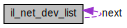
\includegraphics[width=199pt]{structil__net__dev__list__coll__graph}
\end{center}
\end{figure}
\subsection*{Data Fields}
\begin{DoxyCompactItemize}
\item 
char \hyperlink{structil__net__dev__list_afda23220e636423e482e27f89fd0535c}{port} \mbox{[}\hyperlink{group__IL__NET_ga9c33d1c3bf660e4cb980a9e7a676cb88}{I\+L\+\_\+\+N\+E\+T\+\_\+\+P\+O\+R\+T\+\_\+\+SZ}\mbox{]}
\begin{DoxyCompactList}\small\item\em Port. \end{DoxyCompactList}\item 
struct \hyperlink{structil__net__dev__list}{il\+\_\+net\+\_\+dev\+\_\+list} $\ast$ \hyperlink{structil__net__dev__list_a2e1b5a2bd11d369da751960e819272e0}{next}\hypertarget{structil__net__dev__list_a2e1b5a2bd11d369da751960e819272e0}{}\label{structil__net__dev__list_a2e1b5a2bd11d369da751960e819272e0}

\begin{DoxyCompactList}\small\item\em Next device. \end{DoxyCompactList}\end{DoxyCompactItemize}


\subsection{Detailed Description}
network devices list. 

\begin{Desc}
\item[Examples\+: ]\par
\hyperlink{list_8c-example}{list.\+c}.\end{Desc}


\subsection{Field Documentation}
\index{il\+\_\+net\+\_\+dev\+\_\+list@{il\+\_\+net\+\_\+dev\+\_\+list}!port@{port}}
\index{port@{port}!il\+\_\+net\+\_\+dev\+\_\+list@{il\+\_\+net\+\_\+dev\+\_\+list}}
\subsubsection[{\texorpdfstring{port}{port}}]{\setlength{\rightskip}{0pt plus 5cm}char il\+\_\+net\+\_\+dev\+\_\+list\+::port\mbox{[}{\bf I\+L\+\_\+\+N\+E\+T\+\_\+\+P\+O\+R\+T\+\_\+\+SZ}\mbox{]}}\hypertarget{structil__net__dev__list_afda23220e636423e482e27f89fd0535c}{}\label{structil__net__dev__list_afda23220e636423e482e27f89fd0535c}


Port. 

\begin{Desc}
\item[Examples\+: ]\par
\hyperlink{list_8c-example}{list.\+c}.\end{Desc}


The documentation for this struct was generated from the following file\+:\begin{DoxyCompactItemize}
\item 
ingenialink/\hyperlink{net_8h}{net.\+h}\end{DoxyCompactItemize}

\hypertarget{structil__net__opts__t}{}\section{il\+\_\+net\+\_\+opts\+\_\+t Struct Reference}
\label{structil__net__opts__t}\index{il\+\_\+net\+\_\+opts\+\_\+t@{il\+\_\+net\+\_\+opts\+\_\+t}}


Network initialization options.  




{\ttfamily \#include $<$net.\+h$>$}

\subsection*{Data Fields}
\begin{DoxyCompactItemize}
\item 
const char $\ast$ \hyperlink{structil__net__opts__t_a8b65ee2151ffc84031d96eec857a0189}{port}
\begin{DoxyCompactList}\small\item\em Port. \end{DoxyCompactList}\item 
int \hyperlink{structil__net__opts__t_a1fe07477ccaae61b81dd71b2cf4bde08}{timeout\+\_\+rd}
\begin{DoxyCompactList}\small\item\em Read timeout (ms). \end{DoxyCompactList}\item 
int \hyperlink{structil__net__opts__t_a63e3d6b10ac90e08d629ac4458505d1a}{timeout\+\_\+wr}
\begin{DoxyCompactList}\small\item\em Write timeout (ms). \end{DoxyCompactList}\end{DoxyCompactItemize}


\subsection{Detailed Description}
Network initialization options. 

\begin{Desc}
\item[Examples\+: ]\par
\hyperlink{benchmark_8c-example}{benchmark.\+c}, \hyperlink{list_8c-example}{list.\+c}, \hyperlink{monitor_8c-example}{monitor.\+c}, and \hyperlink{servo_monitor_8c-example}{servo\+\_\+monitor.\+c}.\end{Desc}


\subsection{Field Documentation}
\index{il\+\_\+net\+\_\+opts\+\_\+t@{il\+\_\+net\+\_\+opts\+\_\+t}!port@{port}}
\index{port@{port}!il\+\_\+net\+\_\+opts\+\_\+t@{il\+\_\+net\+\_\+opts\+\_\+t}}
\subsubsection[{\texorpdfstring{port}{port}}]{\setlength{\rightskip}{0pt plus 5cm}const char$\ast$ il\+\_\+net\+\_\+opts\+\_\+t\+::port}\hypertarget{structil__net__opts__t_a8b65ee2151ffc84031d96eec857a0189}{}\label{structil__net__opts__t_a8b65ee2151ffc84031d96eec857a0189}


Port. 

\begin{Desc}
\item[Examples\+: ]\par
\hyperlink{benchmark_8c-example}{benchmark.\+c}, \hyperlink{list_8c-example}{list.\+c}, \hyperlink{monitor_8c-example}{monitor.\+c}, and \hyperlink{servo_monitor_8c-example}{servo\+\_\+monitor.\+c}.\end{Desc}
\index{il\+\_\+net\+\_\+opts\+\_\+t@{il\+\_\+net\+\_\+opts\+\_\+t}!timeout\+\_\+rd@{timeout\+\_\+rd}}
\index{timeout\+\_\+rd@{timeout\+\_\+rd}!il\+\_\+net\+\_\+opts\+\_\+t@{il\+\_\+net\+\_\+opts\+\_\+t}}
\subsubsection[{\texorpdfstring{timeout\+\_\+rd}{timeout_rd}}]{\setlength{\rightskip}{0pt plus 5cm}int il\+\_\+net\+\_\+opts\+\_\+t\+::timeout\+\_\+rd}\hypertarget{structil__net__opts__t_a1fe07477ccaae61b81dd71b2cf4bde08}{}\label{structil__net__opts__t_a1fe07477ccaae61b81dd71b2cf4bde08}


Read timeout (ms). 

\begin{Desc}
\item[Examples\+: ]\par
\hyperlink{benchmark_8c-example}{benchmark.\+c}, \hyperlink{list_8c-example}{list.\+c}, \hyperlink{monitor_8c-example}{monitor.\+c}, and \hyperlink{servo_monitor_8c-example}{servo\+\_\+monitor.\+c}.\end{Desc}
\index{il\+\_\+net\+\_\+opts\+\_\+t@{il\+\_\+net\+\_\+opts\+\_\+t}!timeout\+\_\+wr@{timeout\+\_\+wr}}
\index{timeout\+\_\+wr@{timeout\+\_\+wr}!il\+\_\+net\+\_\+opts\+\_\+t@{il\+\_\+net\+\_\+opts\+\_\+t}}
\subsubsection[{\texorpdfstring{timeout\+\_\+wr}{timeout_wr}}]{\setlength{\rightskip}{0pt plus 5cm}int il\+\_\+net\+\_\+opts\+\_\+t\+::timeout\+\_\+wr}\hypertarget{structil__net__opts__t_a63e3d6b10ac90e08d629ac4458505d1a}{}\label{structil__net__opts__t_a63e3d6b10ac90e08d629ac4458505d1a}


Write timeout (ms). 

\begin{Desc}
\item[Examples\+: ]\par
\hyperlink{benchmark_8c-example}{benchmark.\+c}, \hyperlink{list_8c-example}{list.\+c}, \hyperlink{monitor_8c-example}{monitor.\+c}, and \hyperlink{servo_monitor_8c-example}{servo\+\_\+monitor.\+c}.\end{Desc}


The documentation for this struct was generated from the following file\+:\begin{DoxyCompactItemize}
\item 
ingenialink/\hyperlink{net_8h}{net.\+h}\end{DoxyCompactItemize}

\hypertarget{structil__net__servos__list}{}\section{il\+\_\+net\+\_\+servos\+\_\+list Struct Reference}
\label{structil__net__servos__list}\index{il\+\_\+net\+\_\+servos\+\_\+list@{il\+\_\+net\+\_\+servos\+\_\+list}}


Network servos list.  




{\ttfamily \#include $<$net.\+h$>$}



Collaboration diagram for il\+\_\+net\+\_\+servos\+\_\+list\+:\nopagebreak
\begin{figure}[H]
\begin{center}
\leavevmode
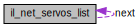
\includegraphics[width=212pt]{structil__net__servos__list__coll__graph}
\end{center}
\end{figure}
\subsection*{Data Fields}
\begin{DoxyCompactItemize}
\item 
uint8\+\_\+t \hyperlink{structil__net__servos__list_a6c8494453cd1a81ddc9cf12d208dc95d}{id}
\begin{DoxyCompactList}\small\item\em Node id. \end{DoxyCompactList}\item 
struct \hyperlink{structil__net__servos__list}{il\+\_\+net\+\_\+servos\+\_\+list} $\ast$ \hyperlink{structil__net__servos__list_a04bbddceab98ab0f7e9cc50a9b46714e}{next}
\begin{DoxyCompactList}\small\item\em Next node. \end{DoxyCompactList}\end{DoxyCompactItemize}


\subsection{Detailed Description}
Network servos list. 

\begin{Desc}
\item[Examples\+: ]\par
\hyperlink{list_8c-example}{list.\+c}, and \hyperlink{servo_monitor_8c-example}{servo\+\_\+monitor.\+c}.\end{Desc}


\subsection{Field Documentation}
\index{il\+\_\+net\+\_\+servos\+\_\+list@{il\+\_\+net\+\_\+servos\+\_\+list}!id@{id}}
\index{id@{id}!il\+\_\+net\+\_\+servos\+\_\+list@{il\+\_\+net\+\_\+servos\+\_\+list}}
\subsubsection[{\texorpdfstring{id}{id}}]{\setlength{\rightskip}{0pt plus 5cm}uint8\+\_\+t il\+\_\+net\+\_\+servos\+\_\+list\+::id}\hypertarget{structil__net__servos__list_a6c8494453cd1a81ddc9cf12d208dc95d}{}\label{structil__net__servos__list_a6c8494453cd1a81ddc9cf12d208dc95d}


Node id. 

\begin{Desc}
\item[Examples\+: ]\par
\hyperlink{list_8c-example}{list.\+c}.\end{Desc}
\index{il\+\_\+net\+\_\+servos\+\_\+list@{il\+\_\+net\+\_\+servos\+\_\+list}!next@{next}}
\index{next@{next}!il\+\_\+net\+\_\+servos\+\_\+list@{il\+\_\+net\+\_\+servos\+\_\+list}}
\subsubsection[{\texorpdfstring{next}{next}}]{\setlength{\rightskip}{0pt plus 5cm}struct {\bf il\+\_\+net\+\_\+servos\+\_\+list}$\ast$ il\+\_\+net\+\_\+servos\+\_\+list\+::next}\hypertarget{structil__net__servos__list_a04bbddceab98ab0f7e9cc50a9b46714e}{}\label{structil__net__servos__list_a04bbddceab98ab0f7e9cc50a9b46714e}


Next node. 



The documentation for this struct was generated from the following file\+:\begin{DoxyCompactItemize}
\item 
ingenialink/\hyperlink{net_8h}{net.\+h}\end{DoxyCompactItemize}

\hypertarget{structil__poller__acq__t}{}\section{il\+\_\+poller\+\_\+acq\+\_\+t Struct Reference}
\label{structil__poller__acq__t}\index{il\+\_\+poller\+\_\+acq\+\_\+t@{il\+\_\+poller\+\_\+acq\+\_\+t}}


Poller acquisition results.  




{\ttfamily \#include $<$poller.\+h$>$}

\subsection*{Data Fields}
\begin{DoxyCompactItemize}
\item 
double $\ast$ \hyperlink{structil__poller__acq__t_aae27ff232752eb21937cefd31c5adcb4}{t}
\begin{DoxyCompactList}\small\item\em Time vector. \end{DoxyCompactList}\item 
double $\ast$$\ast$ \hyperlink{structil__poller__acq__t_aa0c86de89229342ec18f4cf7effdc089}{d}
\begin{DoxyCompactList}\small\item\em Data vectors. \end{DoxyCompactList}\item 
size\+\_\+t \hyperlink{structil__poller__acq__t_aaf726970c22e29aafbbe83d2b24b2eaa}{cnt}
\begin{DoxyCompactList}\small\item\em Number of actual samples in the time and data vectors. \end{DoxyCompactList}\item 
int \hyperlink{structil__poller__acq__t_a41b46fb77cf99d8d2d307e5ec37f707a}{lost}
\begin{DoxyCompactList}\small\item\em Data lost flag. \end{DoxyCompactList}\end{DoxyCompactItemize}


\subsection{Detailed Description}
Poller acquisition results. 

\begin{Desc}
\item[Examples\+: ]\par
\hyperlink{motion_8c-example}{motion.\+c}.\end{Desc}


\subsection{Field Documentation}
\index{il\+\_\+poller\+\_\+acq\+\_\+t@{il\+\_\+poller\+\_\+acq\+\_\+t}!cnt@{cnt}}
\index{cnt@{cnt}!il\+\_\+poller\+\_\+acq\+\_\+t@{il\+\_\+poller\+\_\+acq\+\_\+t}}
\subsubsection[{\texorpdfstring{cnt}{cnt}}]{\setlength{\rightskip}{0pt plus 5cm}size\+\_\+t il\+\_\+poller\+\_\+acq\+\_\+t\+::cnt}\hypertarget{structil__poller__acq__t_aaf726970c22e29aafbbe83d2b24b2eaa}{}\label{structil__poller__acq__t_aaf726970c22e29aafbbe83d2b24b2eaa}


Number of actual samples in the time and data vectors. 

\begin{Desc}
\item[Examples\+: ]\par
\hyperlink{motion_8c-example}{motion.\+c}.\end{Desc}
\index{il\+\_\+poller\+\_\+acq\+\_\+t@{il\+\_\+poller\+\_\+acq\+\_\+t}!d@{d}}
\index{d@{d}!il\+\_\+poller\+\_\+acq\+\_\+t@{il\+\_\+poller\+\_\+acq\+\_\+t}}
\subsubsection[{\texorpdfstring{d}{d}}]{\setlength{\rightskip}{0pt plus 5cm}double$\ast$$\ast$ il\+\_\+poller\+\_\+acq\+\_\+t\+::d}\hypertarget{structil__poller__acq__t_aa0c86de89229342ec18f4cf7effdc089}{}\label{structil__poller__acq__t_aa0c86de89229342ec18f4cf7effdc089}


Data vectors. 

\begin{Desc}
\item[Examples\+: ]\par
\hyperlink{motion_8c-example}{motion.\+c}.\end{Desc}
\index{il\+\_\+poller\+\_\+acq\+\_\+t@{il\+\_\+poller\+\_\+acq\+\_\+t}!lost@{lost}}
\index{lost@{lost}!il\+\_\+poller\+\_\+acq\+\_\+t@{il\+\_\+poller\+\_\+acq\+\_\+t}}
\subsubsection[{\texorpdfstring{lost}{lost}}]{\setlength{\rightskip}{0pt plus 5cm}int il\+\_\+poller\+\_\+acq\+\_\+t\+::lost}\hypertarget{structil__poller__acq__t_a41b46fb77cf99d8d2d307e5ec37f707a}{}\label{structil__poller__acq__t_a41b46fb77cf99d8d2d307e5ec37f707a}


Data lost flag. 

\begin{Desc}
\item[Examples\+: ]\par
\hyperlink{motion_8c-example}{motion.\+c}.\end{Desc}
\index{il\+\_\+poller\+\_\+acq\+\_\+t@{il\+\_\+poller\+\_\+acq\+\_\+t}!t@{t}}
\index{t@{t}!il\+\_\+poller\+\_\+acq\+\_\+t@{il\+\_\+poller\+\_\+acq\+\_\+t}}
\subsubsection[{\texorpdfstring{t}{t}}]{\setlength{\rightskip}{0pt plus 5cm}double$\ast$ il\+\_\+poller\+\_\+acq\+\_\+t\+::t}\hypertarget{structil__poller__acq__t_aae27ff232752eb21937cefd31c5adcb4}{}\label{structil__poller__acq__t_aae27ff232752eb21937cefd31c5adcb4}


Time vector. 

\begin{Desc}
\item[Examples\+: ]\par
\hyperlink{motion_8c-example}{motion.\+c}.\end{Desc}


The documentation for this struct was generated from the following file\+:\begin{DoxyCompactItemize}
\item 
ingenialink/\hyperlink{poller_8h}{poller.\+h}\end{DoxyCompactItemize}

\hypertarget{unionil__reg__limit__t}{}\section{il\+\_\+reg\+\_\+limit\+\_\+t Union Reference}
\label{unionil__reg__limit__t}\index{il\+\_\+reg\+\_\+limit\+\_\+t@{il\+\_\+reg\+\_\+limit\+\_\+t}}


Limits.  




{\ttfamily \#include $<$registers.\+h$>$}

\subsection*{Data Fields}
\begin{DoxyCompactItemize}
\item 
uint8\+\_\+t \hyperlink{unionil__reg__limit__t_aef9083c76539d64e3ca03239a7646f07}{u8}
\begin{DoxyCompactList}\small\item\em Unsigned 8-\/bit value. \end{DoxyCompactList}\item 
int8\+\_\+t \hyperlink{unionil__reg__limit__t_a222839738af51772d82795ec5d625c9c}{s8}
\begin{DoxyCompactList}\small\item\em Signed 8-\/bit value. \end{DoxyCompactList}\item 
uint16\+\_\+t \hyperlink{unionil__reg__limit__t_abdd4796158cab746b84f14e77192f2ec}{u16}
\begin{DoxyCompactList}\small\item\em Unsigned 16-\/bit value. \end{DoxyCompactList}\item 
int16\+\_\+t \hyperlink{unionil__reg__limit__t_a92311f25fb2daa832435239274c5cb2a}{s16}
\begin{DoxyCompactList}\small\item\em Signed 16-\/bit value. \end{DoxyCompactList}\item 
uint32\+\_\+t \hyperlink{unionil__reg__limit__t_a99cf1ff5d5bf0ce76943d15260270211}{u32}
\begin{DoxyCompactList}\small\item\em Unsigned 32-\/bit value. \end{DoxyCompactList}\item 
int32\+\_\+t \hyperlink{unionil__reg__limit__t_a272eb9cd6948fa6137fdef16e4dc9669}{s32}
\begin{DoxyCompactList}\small\item\em Signed 32-\/bit value. \end{DoxyCompactList}\item 
uint64\+\_\+t \hyperlink{unionil__reg__limit__t_aedc5d365162d7f0cf32035695ae0971b}{u64}
\begin{DoxyCompactList}\small\item\em Unsigned 64-\/bit value. \end{DoxyCompactList}\item 
int64\+\_\+t \hyperlink{unionil__reg__limit__t_afb38fc9250bd41f7da4d61a118941d65}{s64}
\begin{DoxyCompactList}\small\item\em Signed 64-\/bit value. \end{DoxyCompactList}\end{DoxyCompactItemize}


\subsection{Detailed Description}
Limits. 



\subsection{Field Documentation}
\index{il\+\_\+reg\+\_\+limit\+\_\+t@{il\+\_\+reg\+\_\+limit\+\_\+t}!s16@{s16}}
\index{s16@{s16}!il\+\_\+reg\+\_\+limit\+\_\+t@{il\+\_\+reg\+\_\+limit\+\_\+t}}
\subsubsection[{\texorpdfstring{s16}{s16}}]{\setlength{\rightskip}{0pt plus 5cm}int16\+\_\+t il\+\_\+reg\+\_\+limit\+\_\+t\+::s16}\hypertarget{unionil__reg__limit__t_a92311f25fb2daa832435239274c5cb2a}{}\label{unionil__reg__limit__t_a92311f25fb2daa832435239274c5cb2a}


Signed 16-\/bit value. 

\begin{Desc}
\item[Examples\+: ]\par
\hyperlink{dict_8c-example}{dict.\+c}.\end{Desc}
\index{il\+\_\+reg\+\_\+limit\+\_\+t@{il\+\_\+reg\+\_\+limit\+\_\+t}!s32@{s32}}
\index{s32@{s32}!il\+\_\+reg\+\_\+limit\+\_\+t@{il\+\_\+reg\+\_\+limit\+\_\+t}}
\subsubsection[{\texorpdfstring{s32}{s32}}]{\setlength{\rightskip}{0pt plus 5cm}int32\+\_\+t il\+\_\+reg\+\_\+limit\+\_\+t\+::s32}\hypertarget{unionil__reg__limit__t_a272eb9cd6948fa6137fdef16e4dc9669}{}\label{unionil__reg__limit__t_a272eb9cd6948fa6137fdef16e4dc9669}


Signed 32-\/bit value. 

\begin{Desc}
\item[Examples\+: ]\par
\hyperlink{dict_8c-example}{dict.\+c}.\end{Desc}
\index{il\+\_\+reg\+\_\+limit\+\_\+t@{il\+\_\+reg\+\_\+limit\+\_\+t}!s64@{s64}}
\index{s64@{s64}!il\+\_\+reg\+\_\+limit\+\_\+t@{il\+\_\+reg\+\_\+limit\+\_\+t}}
\subsubsection[{\texorpdfstring{s64}{s64}}]{\setlength{\rightskip}{0pt plus 5cm}int64\+\_\+t il\+\_\+reg\+\_\+limit\+\_\+t\+::s64}\hypertarget{unionil__reg__limit__t_afb38fc9250bd41f7da4d61a118941d65}{}\label{unionil__reg__limit__t_afb38fc9250bd41f7da4d61a118941d65}


Signed 64-\/bit value. 

\begin{Desc}
\item[Examples\+: ]\par
\hyperlink{dict_8c-example}{dict.\+c}.\end{Desc}
\index{il\+\_\+reg\+\_\+limit\+\_\+t@{il\+\_\+reg\+\_\+limit\+\_\+t}!s8@{s8}}
\index{s8@{s8}!il\+\_\+reg\+\_\+limit\+\_\+t@{il\+\_\+reg\+\_\+limit\+\_\+t}}
\subsubsection[{\texorpdfstring{s8}{s8}}]{\setlength{\rightskip}{0pt plus 5cm}int8\+\_\+t il\+\_\+reg\+\_\+limit\+\_\+t\+::s8}\hypertarget{unionil__reg__limit__t_a222839738af51772d82795ec5d625c9c}{}\label{unionil__reg__limit__t_a222839738af51772d82795ec5d625c9c}


Signed 8-\/bit value. 

\begin{Desc}
\item[Examples\+: ]\par
\hyperlink{dict_8c-example}{dict.\+c}.\end{Desc}
\index{il\+\_\+reg\+\_\+limit\+\_\+t@{il\+\_\+reg\+\_\+limit\+\_\+t}!u16@{u16}}
\index{u16@{u16}!il\+\_\+reg\+\_\+limit\+\_\+t@{il\+\_\+reg\+\_\+limit\+\_\+t}}
\subsubsection[{\texorpdfstring{u16}{u16}}]{\setlength{\rightskip}{0pt plus 5cm}uint16\+\_\+t il\+\_\+reg\+\_\+limit\+\_\+t\+::u16}\hypertarget{unionil__reg__limit__t_abdd4796158cab746b84f14e77192f2ec}{}\label{unionil__reg__limit__t_abdd4796158cab746b84f14e77192f2ec}


Unsigned 16-\/bit value. 

\begin{Desc}
\item[Examples\+: ]\par
\hyperlink{dict_8c-example}{dict.\+c}.\end{Desc}
\index{il\+\_\+reg\+\_\+limit\+\_\+t@{il\+\_\+reg\+\_\+limit\+\_\+t}!u32@{u32}}
\index{u32@{u32}!il\+\_\+reg\+\_\+limit\+\_\+t@{il\+\_\+reg\+\_\+limit\+\_\+t}}
\subsubsection[{\texorpdfstring{u32}{u32}}]{\setlength{\rightskip}{0pt plus 5cm}uint32\+\_\+t il\+\_\+reg\+\_\+limit\+\_\+t\+::u32}\hypertarget{unionil__reg__limit__t_a99cf1ff5d5bf0ce76943d15260270211}{}\label{unionil__reg__limit__t_a99cf1ff5d5bf0ce76943d15260270211}


Unsigned 32-\/bit value. 

\begin{Desc}
\item[Examples\+: ]\par
\hyperlink{dict_8c-example}{dict.\+c}.\end{Desc}
\index{il\+\_\+reg\+\_\+limit\+\_\+t@{il\+\_\+reg\+\_\+limit\+\_\+t}!u64@{u64}}
\index{u64@{u64}!il\+\_\+reg\+\_\+limit\+\_\+t@{il\+\_\+reg\+\_\+limit\+\_\+t}}
\subsubsection[{\texorpdfstring{u64}{u64}}]{\setlength{\rightskip}{0pt plus 5cm}uint64\+\_\+t il\+\_\+reg\+\_\+limit\+\_\+t\+::u64}\hypertarget{unionil__reg__limit__t_aedc5d365162d7f0cf32035695ae0971b}{}\label{unionil__reg__limit__t_aedc5d365162d7f0cf32035695ae0971b}


Unsigned 64-\/bit value. 

\begin{Desc}
\item[Examples\+: ]\par
\hyperlink{dict_8c-example}{dict.\+c}.\end{Desc}
\index{il\+\_\+reg\+\_\+limit\+\_\+t@{il\+\_\+reg\+\_\+limit\+\_\+t}!u8@{u8}}
\index{u8@{u8}!il\+\_\+reg\+\_\+limit\+\_\+t@{il\+\_\+reg\+\_\+limit\+\_\+t}}
\subsubsection[{\texorpdfstring{u8}{u8}}]{\setlength{\rightskip}{0pt plus 5cm}uint8\+\_\+t il\+\_\+reg\+\_\+limit\+\_\+t\+::u8}\hypertarget{unionil__reg__limit__t_aef9083c76539d64e3ca03239a7646f07}{}\label{unionil__reg__limit__t_aef9083c76539d64e3ca03239a7646f07}


Unsigned 8-\/bit value. 

\begin{Desc}
\item[Examples\+: ]\par
\hyperlink{dict_8c-example}{dict.\+c}.\end{Desc}


The documentation for this union was generated from the following file\+:\begin{DoxyCompactItemize}
\item 
ingenialink/\hyperlink{registers_8h}{registers.\+h}\end{DoxyCompactItemize}

\hypertarget{structil__reg__range__t}{}\section{il\+\_\+reg\+\_\+range\+\_\+t Struct Reference}
\label{structil__reg__range__t}\index{il\+\_\+reg\+\_\+range\+\_\+t@{il\+\_\+reg\+\_\+range\+\_\+t}}


Range.  




{\ttfamily \#include $<$registers.\+h$>$}



Collaboration diagram for il\+\_\+reg\+\_\+range\+\_\+t\+:\nopagebreak
\begin{figure}[H]
\begin{center}
\leavevmode
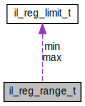
\includegraphics[width=157pt]{structil__reg__range__t__coll__graph}
\end{center}
\end{figure}
\subsection*{Data Fields}
\begin{DoxyCompactItemize}
\item 
\hyperlink{unionil__reg__limit__t}{il\+\_\+reg\+\_\+limit\+\_\+t} \hyperlink{structil__reg__range__t_a5f2d3034108ba4f003dea87baaccf19c}{min}
\begin{DoxyCompactList}\small\item\em Minimum. \end{DoxyCompactList}\item 
\hyperlink{unionil__reg__limit__t}{il\+\_\+reg\+\_\+limit\+\_\+t} \hyperlink{structil__reg__range__t_aea6987fad601c38802c00a67027de135}{max}
\begin{DoxyCompactList}\small\item\em Maximum. \end{DoxyCompactList}\end{DoxyCompactItemize}


\subsection{Detailed Description}
Range. 



\subsection{Field Documentation}
\index{il\+\_\+reg\+\_\+range\+\_\+t@{il\+\_\+reg\+\_\+range\+\_\+t}!max@{max}}
\index{max@{max}!il\+\_\+reg\+\_\+range\+\_\+t@{il\+\_\+reg\+\_\+range\+\_\+t}}
\subsubsection[{\texorpdfstring{max}{max}}]{\setlength{\rightskip}{0pt plus 5cm}{\bf il\+\_\+reg\+\_\+limit\+\_\+t} il\+\_\+reg\+\_\+range\+\_\+t\+::max}\hypertarget{structil__reg__range__t_aea6987fad601c38802c00a67027de135}{}\label{structil__reg__range__t_aea6987fad601c38802c00a67027de135}


Maximum. 

\begin{Desc}
\item[Examples\+: ]\par
\hyperlink{dict_8c-example}{dict.\+c}.\end{Desc}
\index{il\+\_\+reg\+\_\+range\+\_\+t@{il\+\_\+reg\+\_\+range\+\_\+t}!min@{min}}
\index{min@{min}!il\+\_\+reg\+\_\+range\+\_\+t@{il\+\_\+reg\+\_\+range\+\_\+t}}
\subsubsection[{\texorpdfstring{min}{min}}]{\setlength{\rightskip}{0pt plus 5cm}{\bf il\+\_\+reg\+\_\+limit\+\_\+t} il\+\_\+reg\+\_\+range\+\_\+t\+::min}\hypertarget{structil__reg__range__t_a5f2d3034108ba4f003dea87baaccf19c}{}\label{structil__reg__range__t_a5f2d3034108ba4f003dea87baaccf19c}


Minimum. 

\begin{Desc}
\item[Examples\+: ]\par
\hyperlink{dict_8c-example}{dict.\+c}.\end{Desc}


The documentation for this struct was generated from the following file\+:\begin{DoxyCompactItemize}
\item 
ingenialink/\hyperlink{registers_8h}{registers.\+h}\end{DoxyCompactItemize}

\hypertarget{structil__reg__t}{}\section{il\+\_\+reg\+\_\+t Struct Reference}
\label{structil__reg__t}\index{il\+\_\+reg\+\_\+t@{il\+\_\+reg\+\_\+t}}


Register.  




{\ttfamily \#include $<$registers.\+h$>$}



Collaboration diagram for il\+\_\+reg\+\_\+t\+:\nopagebreak
\begin{figure}[H]
\begin{center}
\leavevmode
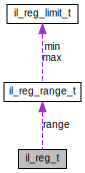
\includegraphics[width=157pt]{structil__reg__t__coll__graph}
\end{center}
\end{figure}
\subsection*{Data Fields}
\begin{DoxyCompactItemize}
\item 
uint32\+\_\+t \hyperlink{structil__reg__t_ac0433a8ae86e0990fa59a074a5ad1bd1}{address}
\begin{DoxyCompactList}\small\item\em Address. \end{DoxyCompactList}\item 
\hyperlink{group__IL__REGS_gaddd7edef254d348f2e8a48c40840cdd6}{il\+\_\+reg\+\_\+dtype\+\_\+t} \hyperlink{structil__reg__t_a1780caa197277828816c7214aa7b5d2f}{dtype}
\begin{DoxyCompactList}\small\item\em Data type. \end{DoxyCompactList}\item 
\hyperlink{group__IL__REGS_ga4c623bd7d0d5f059dd91949c6948147e}{il\+\_\+reg\+\_\+access\+\_\+t} \hyperlink{structil__reg__t_a8cd718765e48f0de2f978de386c61218}{access}
\begin{DoxyCompactList}\small\item\em Access type. \end{DoxyCompactList}\item 
\hyperlink{group__IL__REGS_ga37538453e5c3d84733c628987a579590}{il\+\_\+reg\+\_\+phy\+\_\+t} \hyperlink{structil__reg__t_a799847eb04e4f29073e7c9939ae977df}{phy}
\begin{DoxyCompactList}\small\item\em Physical units type. \end{DoxyCompactList}\item 
\hyperlink{structil__reg__range__t}{il\+\_\+reg\+\_\+range\+\_\+t} \hyperlink{structil__reg__t_acb9979e9f542ec4b683a6b2b603d4bea}{range}
\begin{DoxyCompactList}\small\item\em Range. \end{DoxyCompactList}\item 
\hyperlink{group__IL__DICT__LABELS_ga69d1109256f465cbcfa8aac7fa592495}{il\+\_\+dict\+\_\+labels\+\_\+t} $\ast$ \hyperlink{structil__reg__t_a6d86137472a9c21c1c364f05c58b943b}{labels}
\begin{DoxyCompactList}\small\item\em Labels dictionary. \end{DoxyCompactList}\item 
const char $\ast$ \hyperlink{structil__reg__t_a9306d321ecedb9559d7dd339c6115b78}{cat\+\_\+id}
\begin{DoxyCompactList}\small\item\em Category ID. \end{DoxyCompactList}\item 
const char $\ast$ \hyperlink{structil__reg__t_a827bdfd4438dc720a322ec17c17afe2f}{scat\+\_\+id}
\begin{DoxyCompactList}\small\item\em Subcategory ID. \end{DoxyCompactList}\end{DoxyCompactItemize}


\subsection{Detailed Description}
Register. 

\begin{Desc}
\item[Examples\+: ]\par
\hyperlink{benchmark_8c-example}{benchmark.\+c}, \hyperlink{dict_8c-example}{dict.\+c}, \hyperlink{monitor_8c-example}{monitor.\+c}, and \hyperlink{motion_8c-example}{motion.\+c}.\end{Desc}


\subsection{Field Documentation}
\index{il\+\_\+reg\+\_\+t@{il\+\_\+reg\+\_\+t}!access@{access}}
\index{access@{access}!il\+\_\+reg\+\_\+t@{il\+\_\+reg\+\_\+t}}
\subsubsection[{\texorpdfstring{access}{access}}]{\setlength{\rightskip}{0pt plus 5cm}{\bf il\+\_\+reg\+\_\+access\+\_\+t} il\+\_\+reg\+\_\+t\+::access}\hypertarget{structil__reg__t_a8cd718765e48f0de2f978de386c61218}{}\label{structil__reg__t_a8cd718765e48f0de2f978de386c61218}


Access type. 

\begin{Desc}
\item[Examples\+: ]\par
\hyperlink{benchmark_8c-example}{benchmark.\+c}, and \hyperlink{dict_8c-example}{dict.\+c}.\end{Desc}
\index{il\+\_\+reg\+\_\+t@{il\+\_\+reg\+\_\+t}!address@{address}}
\index{address@{address}!il\+\_\+reg\+\_\+t@{il\+\_\+reg\+\_\+t}}
\subsubsection[{\texorpdfstring{address}{address}}]{\setlength{\rightskip}{0pt plus 5cm}uint32\+\_\+t il\+\_\+reg\+\_\+t\+::address}\hypertarget{structil__reg__t_ac0433a8ae86e0990fa59a074a5ad1bd1}{}\label{structil__reg__t_ac0433a8ae86e0990fa59a074a5ad1bd1}


Address. 

\begin{Desc}
\item[Examples\+: ]\par
\hyperlink{benchmark_8c-example}{benchmark.\+c}, \hyperlink{dict_8c-example}{dict.\+c}, \hyperlink{monitor_8c-example}{monitor.\+c}, and \hyperlink{motion_8c-example}{motion.\+c}.\end{Desc}
\index{il\+\_\+reg\+\_\+t@{il\+\_\+reg\+\_\+t}!cat\+\_\+id@{cat\+\_\+id}}
\index{cat\+\_\+id@{cat\+\_\+id}!il\+\_\+reg\+\_\+t@{il\+\_\+reg\+\_\+t}}
\subsubsection[{\texorpdfstring{cat\+\_\+id}{cat_id}}]{\setlength{\rightskip}{0pt plus 5cm}const char$\ast$ il\+\_\+reg\+\_\+t\+::cat\+\_\+id}\hypertarget{structil__reg__t_a9306d321ecedb9559d7dd339c6115b78}{}\label{structil__reg__t_a9306d321ecedb9559d7dd339c6115b78}


Category ID. 

\begin{Desc}
\item[Examples\+: ]\par
\hyperlink{dict_8c-example}{dict.\+c}.\end{Desc}
\index{il\+\_\+reg\+\_\+t@{il\+\_\+reg\+\_\+t}!dtype@{dtype}}
\index{dtype@{dtype}!il\+\_\+reg\+\_\+t@{il\+\_\+reg\+\_\+t}}
\subsubsection[{\texorpdfstring{dtype}{dtype}}]{\setlength{\rightskip}{0pt plus 5cm}{\bf il\+\_\+reg\+\_\+dtype\+\_\+t} il\+\_\+reg\+\_\+t\+::dtype}\hypertarget{structil__reg__t_a1780caa197277828816c7214aa7b5d2f}{}\label{structil__reg__t_a1780caa197277828816c7214aa7b5d2f}


Data type. 

\begin{Desc}
\item[Examples\+: ]\par
\hyperlink{benchmark_8c-example}{benchmark.\+c}, and \hyperlink{dict_8c-example}{dict.\+c}.\end{Desc}
\index{il\+\_\+reg\+\_\+t@{il\+\_\+reg\+\_\+t}!labels@{labels}}
\index{labels@{labels}!il\+\_\+reg\+\_\+t@{il\+\_\+reg\+\_\+t}}
\subsubsection[{\texorpdfstring{labels}{labels}}]{\setlength{\rightskip}{0pt plus 5cm}{\bf il\+\_\+dict\+\_\+labels\+\_\+t}$\ast$ il\+\_\+reg\+\_\+t\+::labels}\hypertarget{structil__reg__t_a6d86137472a9c21c1c364f05c58b943b}{}\label{structil__reg__t_a6d86137472a9c21c1c364f05c58b943b}


Labels dictionary. 

\begin{Desc}
\item[Examples\+: ]\par
\hyperlink{dict_8c-example}{dict.\+c}.\end{Desc}
\index{il\+\_\+reg\+\_\+t@{il\+\_\+reg\+\_\+t}!phy@{phy}}
\index{phy@{phy}!il\+\_\+reg\+\_\+t@{il\+\_\+reg\+\_\+t}}
\subsubsection[{\texorpdfstring{phy}{phy}}]{\setlength{\rightskip}{0pt plus 5cm}{\bf il\+\_\+reg\+\_\+phy\+\_\+t} il\+\_\+reg\+\_\+t\+::phy}\hypertarget{structil__reg__t_a799847eb04e4f29073e7c9939ae977df}{}\label{structil__reg__t_a799847eb04e4f29073e7c9939ae977df}


Physical units type. 

\begin{Desc}
\item[Examples\+: ]\par
\hyperlink{benchmark_8c-example}{benchmark.\+c}, and \hyperlink{dict_8c-example}{dict.\+c}.\end{Desc}
\index{il\+\_\+reg\+\_\+t@{il\+\_\+reg\+\_\+t}!range@{range}}
\index{range@{range}!il\+\_\+reg\+\_\+t@{il\+\_\+reg\+\_\+t}}
\subsubsection[{\texorpdfstring{range}{range}}]{\setlength{\rightskip}{0pt plus 5cm}{\bf il\+\_\+reg\+\_\+range\+\_\+t} il\+\_\+reg\+\_\+t\+::range}\hypertarget{structil__reg__t_acb9979e9f542ec4b683a6b2b603d4bea}{}\label{structil__reg__t_acb9979e9f542ec4b683a6b2b603d4bea}


Range. 

\begin{Desc}
\item[Examples\+: ]\par
\hyperlink{dict_8c-example}{dict.\+c}.\end{Desc}
\index{il\+\_\+reg\+\_\+t@{il\+\_\+reg\+\_\+t}!scat\+\_\+id@{scat\+\_\+id}}
\index{scat\+\_\+id@{scat\+\_\+id}!il\+\_\+reg\+\_\+t@{il\+\_\+reg\+\_\+t}}
\subsubsection[{\texorpdfstring{scat\+\_\+id}{scat_id}}]{\setlength{\rightskip}{0pt plus 5cm}const char$\ast$ il\+\_\+reg\+\_\+t\+::scat\+\_\+id}\hypertarget{structil__reg__t_a827bdfd4438dc720a322ec17c17afe2f}{}\label{structil__reg__t_a827bdfd4438dc720a322ec17c17afe2f}


Subcategory ID. 

\begin{Desc}
\item[Examples\+: ]\par
\hyperlink{dict_8c-example}{dict.\+c}.\end{Desc}


The documentation for this struct was generated from the following file\+:\begin{DoxyCompactItemize}
\item 
ingenialink/\hyperlink{registers_8h}{registers.\+h}\end{DoxyCompactItemize}

\hypertarget{structil__servo__info__t}{}\section{il\+\_\+servo\+\_\+info\+\_\+t Struct Reference}
\label{structil__servo__info__t}\index{il\+\_\+servo\+\_\+info\+\_\+t@{il\+\_\+servo\+\_\+info\+\_\+t}}


Ingenia\+Link servo information.  




{\ttfamily \#include $<$servo.\+h$>$}

\subsection*{Data Fields}
\begin{DoxyCompactItemize}
\item 
uint32\+\_\+t \hyperlink{structil__servo__info__t_a0ae637a9d167672496e381e23c5cd5d5}{serial}
\begin{DoxyCompactList}\small\item\em Serial. \end{DoxyCompactList}\item 
char \hyperlink{structil__servo__info__t_a1499b7681107bb0310f353615f9ea6d6}{name} \mbox{[}\hyperlink{group__IL__SERVO_ga0a684ea427841d8ba4cf87b2d9a94d97}{I\+L\+\_\+\+S\+E\+R\+V\+O\+\_\+\+N\+A\+M\+E\+\_\+\+SZ}\mbox{]}
\begin{DoxyCompactList}\small\item\em Name. \end{DoxyCompactList}\item 
char \hyperlink{structil__servo__info__t_ad08af6ad43a8c261812fa9775bc4fc08}{sw\+\_\+version} \mbox{[}\hyperlink{group__IL__SERVO_gaec19ad2892772d99664f16c55b9bc43f}{I\+L\+\_\+\+S\+E\+R\+V\+O\+\_\+\+S\+W\+\_\+\+V\+E\+R\+S\+I\+O\+N\+\_\+\+SZ}\mbox{]}
\begin{DoxyCompactList}\small\item\em Software version. \end{DoxyCompactList}\item 
char \hyperlink{structil__servo__info__t_abd47e38a9b25fd17f1dfb09341a83c93}{hw\+\_\+variant} \mbox{[}\hyperlink{group__IL__SERVO_ga18d9729ab800ffdda8ec81d8146a7e3f}{I\+L\+\_\+\+S\+E\+R\+V\+O\+\_\+\+H\+W\+\_\+\+V\+A\+R\+I\+A\+N\+T\+\_\+\+SZ}\mbox{]}
\begin{DoxyCompactList}\small\item\em Hardware variant. \end{DoxyCompactList}\item 
uint32\+\_\+t \hyperlink{structil__servo__info__t_a5faaa1ff2b81386dfe159650ba85a0be}{prod\+\_\+code}
\begin{DoxyCompactList}\small\item\em Product code. \end{DoxyCompactList}\item 
uint32\+\_\+t \hyperlink{structil__servo__info__t_abfec53fe057b8a4a5fa79d02be777643}{revision}
\begin{DoxyCompactList}\small\item\em Revision number. \end{DoxyCompactList}\end{DoxyCompactItemize}


\subsection{Detailed Description}
Ingenia\+Link servo information. 

\begin{Desc}
\item[Examples\+: ]\par
\hyperlink{list_8c-example}{list.\+c}.\end{Desc}


\subsection{Field Documentation}
\index{il\+\_\+servo\+\_\+info\+\_\+t@{il\+\_\+servo\+\_\+info\+\_\+t}!hw\+\_\+variant@{hw\+\_\+variant}}
\index{hw\+\_\+variant@{hw\+\_\+variant}!il\+\_\+servo\+\_\+info\+\_\+t@{il\+\_\+servo\+\_\+info\+\_\+t}}
\subsubsection[{\texorpdfstring{hw\+\_\+variant}{hw_variant}}]{\setlength{\rightskip}{0pt plus 5cm}char il\+\_\+servo\+\_\+info\+\_\+t\+::hw\+\_\+variant\mbox{[}{\bf I\+L\+\_\+\+S\+E\+R\+V\+O\+\_\+\+H\+W\+\_\+\+V\+A\+R\+I\+A\+N\+T\+\_\+\+SZ}\mbox{]}}\hypertarget{structil__servo__info__t_abd47e38a9b25fd17f1dfb09341a83c93}{}\label{structil__servo__info__t_abd47e38a9b25fd17f1dfb09341a83c93}


Hardware variant. 

\begin{Desc}
\item[Examples\+: ]\par
\hyperlink{list_8c-example}{list.\+c}.\end{Desc}
\index{il\+\_\+servo\+\_\+info\+\_\+t@{il\+\_\+servo\+\_\+info\+\_\+t}!name@{name}}
\index{name@{name}!il\+\_\+servo\+\_\+info\+\_\+t@{il\+\_\+servo\+\_\+info\+\_\+t}}
\subsubsection[{\texorpdfstring{name}{name}}]{\setlength{\rightskip}{0pt plus 5cm}char il\+\_\+servo\+\_\+info\+\_\+t\+::name\mbox{[}{\bf I\+L\+\_\+\+S\+E\+R\+V\+O\+\_\+\+N\+A\+M\+E\+\_\+\+SZ}\mbox{]}}\hypertarget{structil__servo__info__t_a1499b7681107bb0310f353615f9ea6d6}{}\label{structil__servo__info__t_a1499b7681107bb0310f353615f9ea6d6}


Name. 

\begin{Desc}
\item[Examples\+: ]\par
\hyperlink{list_8c-example}{list.\+c}.\end{Desc}
\index{il\+\_\+servo\+\_\+info\+\_\+t@{il\+\_\+servo\+\_\+info\+\_\+t}!prod\+\_\+code@{prod\+\_\+code}}
\index{prod\+\_\+code@{prod\+\_\+code}!il\+\_\+servo\+\_\+info\+\_\+t@{il\+\_\+servo\+\_\+info\+\_\+t}}
\subsubsection[{\texorpdfstring{prod\+\_\+code}{prod_code}}]{\setlength{\rightskip}{0pt plus 5cm}uint32\+\_\+t il\+\_\+servo\+\_\+info\+\_\+t\+::prod\+\_\+code}\hypertarget{structil__servo__info__t_a5faaa1ff2b81386dfe159650ba85a0be}{}\label{structil__servo__info__t_a5faaa1ff2b81386dfe159650ba85a0be}


Product code. 

\begin{Desc}
\item[Examples\+: ]\par
\hyperlink{list_8c-example}{list.\+c}.\end{Desc}
\index{il\+\_\+servo\+\_\+info\+\_\+t@{il\+\_\+servo\+\_\+info\+\_\+t}!revision@{revision}}
\index{revision@{revision}!il\+\_\+servo\+\_\+info\+\_\+t@{il\+\_\+servo\+\_\+info\+\_\+t}}
\subsubsection[{\texorpdfstring{revision}{revision}}]{\setlength{\rightskip}{0pt plus 5cm}uint32\+\_\+t il\+\_\+servo\+\_\+info\+\_\+t\+::revision}\hypertarget{structil__servo__info__t_abfec53fe057b8a4a5fa79d02be777643}{}\label{structil__servo__info__t_abfec53fe057b8a4a5fa79d02be777643}


Revision number. 

\begin{Desc}
\item[Examples\+: ]\par
\hyperlink{list_8c-example}{list.\+c}.\end{Desc}
\index{il\+\_\+servo\+\_\+info\+\_\+t@{il\+\_\+servo\+\_\+info\+\_\+t}!serial@{serial}}
\index{serial@{serial}!il\+\_\+servo\+\_\+info\+\_\+t@{il\+\_\+servo\+\_\+info\+\_\+t}}
\subsubsection[{\texorpdfstring{serial}{serial}}]{\setlength{\rightskip}{0pt plus 5cm}uint32\+\_\+t il\+\_\+servo\+\_\+info\+\_\+t\+::serial}\hypertarget{structil__servo__info__t_a0ae637a9d167672496e381e23c5cd5d5}{}\label{structil__servo__info__t_a0ae637a9d167672496e381e23c5cd5d5}


Serial. 

\begin{Desc}
\item[Examples\+: ]\par
\hyperlink{list_8c-example}{list.\+c}.\end{Desc}
\index{il\+\_\+servo\+\_\+info\+\_\+t@{il\+\_\+servo\+\_\+info\+\_\+t}!sw\+\_\+version@{sw\+\_\+version}}
\index{sw\+\_\+version@{sw\+\_\+version}!il\+\_\+servo\+\_\+info\+\_\+t@{il\+\_\+servo\+\_\+info\+\_\+t}}
\subsubsection[{\texorpdfstring{sw\+\_\+version}{sw_version}}]{\setlength{\rightskip}{0pt plus 5cm}char il\+\_\+servo\+\_\+info\+\_\+t\+::sw\+\_\+version\mbox{[}{\bf I\+L\+\_\+\+S\+E\+R\+V\+O\+\_\+\+S\+W\+\_\+\+V\+E\+R\+S\+I\+O\+N\+\_\+\+SZ}\mbox{]}}\hypertarget{structil__servo__info__t_ad08af6ad43a8c261812fa9775bc4fc08}{}\label{structil__servo__info__t_ad08af6ad43a8c261812fa9775bc4fc08}


Software version. 

\begin{Desc}
\item[Examples\+: ]\par
\hyperlink{list_8c-example}{list.\+c}.\end{Desc}


The documentation for this struct was generated from the following file\+:\begin{DoxyCompactItemize}
\item 
ingenialink/\hyperlink{servo_8h}{servo.\+h}\end{DoxyCompactItemize}

\chapter{File Documentation}
\hypertarget{common_8h}{}\section{ingenialink/common.h File Reference}
\label{common_8h}\index{ingenialink/common.\+h@{ingenialink/common.\+h}}


Common.  


{\ttfamily \#include \char`\"{}config.\+h\char`\"{}}\\*
{\ttfamily \#include $<$stdlib.\+h$>$}\\*
{\ttfamily \#include $<$stdint.\+h$>$}\\*
Include dependency graph for common.\+h\+:\nopagebreak
\begin{figure}[H]
\begin{center}
\leavevmode
\includegraphics[width=265pt]{common_8h__incl}
\end{center}
\end{figure}
This graph shows which files directly or indirectly include this file\+:\nopagebreak
\begin{figure}[H]
\begin{center}
\leavevmode
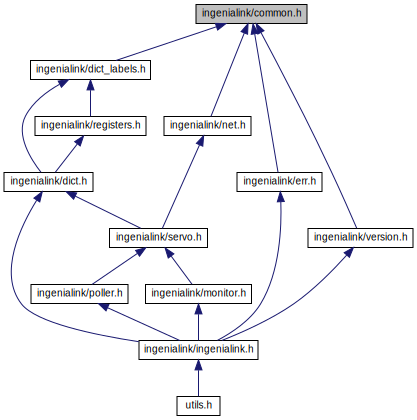
\includegraphics[width=350pt]{common_8h__dep__incl}
\end{center}
\end{figure}
\subsection*{Macros}
{\bf }\par
\begin{DoxyCompactItemize}
\item 
\#define \hyperlink{common_8h_ae9e1f6ce0f3ab55bd128dced2412c024}{I\+L\+\_\+\+B\+E\+G\+I\+N\+\_\+\+D\+E\+CL}
\begin{DoxyCompactList}\small\item\em Start declaration in C mode. \end{DoxyCompactList}\item 
\#define \hyperlink{common_8h_aa4cc50eed54c21cfcd7764272a618e35}{I\+L\+\_\+\+E\+N\+D\+\_\+\+D\+E\+CL}
\begin{DoxyCompactList}\small\item\em End declaration in C mode. \end{DoxyCompactList}\item 
\#define \hyperlink{common_8h_a6bb629d26c52bfe10519ba3176853f47}{I\+L\+\_\+\+E\+X\+P\+O\+RT}
\begin{DoxyCompactList}\small\item\em Declare a public function exported for application use. \end{DoxyCompactList}\end{DoxyCompactItemize}



\subsection{Detailed Description}
Common. 



\subsection{Macro Definition Documentation}
\index{common.\+h@{common.\+h}!I\+L\+\_\+\+B\+E\+G\+I\+N\+\_\+\+D\+E\+CL@{I\+L\+\_\+\+B\+E\+G\+I\+N\+\_\+\+D\+E\+CL}}
\index{I\+L\+\_\+\+B\+E\+G\+I\+N\+\_\+\+D\+E\+CL@{I\+L\+\_\+\+B\+E\+G\+I\+N\+\_\+\+D\+E\+CL}!common.\+h@{common.\+h}}
\subsubsection[{\texorpdfstring{I\+L\+\_\+\+B\+E\+G\+I\+N\+\_\+\+D\+E\+CL}{IL_BEGIN_DECL}}]{\setlength{\rightskip}{0pt plus 5cm}\#define I\+L\+\_\+\+B\+E\+G\+I\+N\+\_\+\+D\+E\+CL}\hypertarget{common_8h_ae9e1f6ce0f3ab55bd128dced2412c024}{}\label{common_8h_ae9e1f6ce0f3ab55bd128dced2412c024}


Start declaration in C mode. 

\index{common.\+h@{common.\+h}!I\+L\+\_\+\+E\+N\+D\+\_\+\+D\+E\+CL@{I\+L\+\_\+\+E\+N\+D\+\_\+\+D\+E\+CL}}
\index{I\+L\+\_\+\+E\+N\+D\+\_\+\+D\+E\+CL@{I\+L\+\_\+\+E\+N\+D\+\_\+\+D\+E\+CL}!common.\+h@{common.\+h}}
\subsubsection[{\texorpdfstring{I\+L\+\_\+\+E\+N\+D\+\_\+\+D\+E\+CL}{IL_END_DECL}}]{\setlength{\rightskip}{0pt plus 5cm}\#define I\+L\+\_\+\+E\+N\+D\+\_\+\+D\+E\+CL}\hypertarget{common_8h_aa4cc50eed54c21cfcd7764272a618e35}{}\label{common_8h_aa4cc50eed54c21cfcd7764272a618e35}


End declaration in C mode. 

\index{common.\+h@{common.\+h}!I\+L\+\_\+\+E\+X\+P\+O\+RT@{I\+L\+\_\+\+E\+X\+P\+O\+RT}}
\index{I\+L\+\_\+\+E\+X\+P\+O\+RT@{I\+L\+\_\+\+E\+X\+P\+O\+RT}!common.\+h@{common.\+h}}
\subsubsection[{\texorpdfstring{I\+L\+\_\+\+E\+X\+P\+O\+RT}{IL_EXPORT}}]{\setlength{\rightskip}{0pt plus 5cm}\#define I\+L\+\_\+\+E\+X\+P\+O\+RT}\hypertarget{common_8h_a6bb629d26c52bfe10519ba3176853f47}{}\label{common_8h_a6bb629d26c52bfe10519ba3176853f47}


Declare a public function exported for application use. 


\hypertarget{const_8h}{}\section{ingenialink/const.h File Reference}
\label{const_8h}\index{ingenialink/const.\+h@{ingenialink/const.\+h}}


Constants.  


This graph shows which files directly or indirectly include this file\+:\nopagebreak
\begin{figure}[H]
\begin{center}
\leavevmode
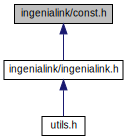
\includegraphics[width=199pt]{const_8h__dep__incl}
\end{center}
\end{figure}
\subsection*{Macros}
\begin{DoxyCompactItemize}
\item 
\#define \hyperlink{group__IL__CONST__SYS_gaefbce026149e3fd1ca4912e8b831e1c0}{I\+L\+K\+\_\+\+S\+Y\+S\+\_\+\+P\+W\+M\+\_\+\+M\+AX}~32767
\begin{DoxyCompactList}\small\item\em P\+WM maximum value (maximum of signed 16-\/bit). \end{DoxyCompactList}\item 
\#define \hyperlink{group__IL__CONST__SYS_gaebdf8cd11949f44b6f98507754e2eda5}{I\+L\+K\+\_\+\+S\+Y\+S\+\_\+\+C\+L\+O\+O\+P\+\_\+\+F\+R\+E\+Q\+\_\+\+T\+O\+R\+Q\+UE}~10000
\begin{DoxyCompactList}\small\item\em Current/\+Torque loop frequency (Hz). \end{DoxyCompactList}\item 
\#define \hyperlink{group__IL__CONST__SYS_gab7567b15639de41f00debc89e8cf69c1}{I\+L\+K\+\_\+\+S\+Y\+S\+\_\+\+C\+L\+O\+O\+P\+\_\+\+F\+R\+E\+Q\+\_\+\+V\+EL}~1000
\begin{DoxyCompactList}\small\item\em Velocity loop frequency (Hz). \end{DoxyCompactList}\item 
\#define \hyperlink{group__IL__CONST__SYS_ga0936a074e3c6022add3b4dd936d7472e}{I\+L\+K\+\_\+\+S\+Y\+S\+\_\+\+C\+L\+O\+O\+P\+\_\+\+F\+R\+E\+Q\+\_\+\+P\+OS}~1000
\begin{DoxyCompactList}\small\item\em Position loop frequency (Hz). \end{DoxyCompactList}\item 
\#define \hyperlink{group__IL__CONST__SYS_ga7d97997e842304310662f2b151281a9f}{I\+L\+K\+\_\+\+S\+Y\+S\+\_\+\+T\+O\+R\+Q\+U\+E\+\_\+\+M\+AX}~32767
\begin{DoxyCompactList}\small\item\em Maximum rated torque (maximum of I\+N\+T16). \end{DoxyCompactList}\item 
\#define \hyperlink{group__IL__CONST__SYS_ga67fd909fd6fa467e246a1d03aaaab058}{I\+L\+K\+\_\+\+S\+Y\+S\+\_\+\+D\+S\+I\+G\+\_\+\+M\+A\+X\+\_\+\+S\+A\+M\+P\+L\+ES}~1000
\begin{DoxyCompactList}\small\item\em Disturbance signal maximum samples. \end{DoxyCompactList}\item 
\#define \hyperlink{group__IL__CONST__SIGNATURES_ga4c86aee7016ece956e15b5d1523fbc07}{I\+L\+K\+\_\+\+S\+I\+G\+N\+A\+T\+U\+R\+E\+\_\+\+S\+T\+O\+RE}~0x65766173
\begin{DoxyCompactList}\small\item\em Store signature. \end{DoxyCompactList}\item 
\#define \hyperlink{group__IL__CONST__SIGNATURES_gafec6f03943f9194696a21de117dedbfc}{I\+L\+K\+\_\+\+S\+I\+G\+N\+A\+T\+U\+R\+E\+\_\+\+R\+E\+S\+ET}~0x64747372
\begin{DoxyCompactList}\small\item\em Reset signature. \end{DoxyCompactList}\item 
\#define \hyperlink{group__IL__CONST__OP__MODE_ga1f22e168e8a3092acf6982d6374ef829}{I\+L\+K\+\_\+\+O\+P\+\_\+\+M\+O\+D\+E\+\_\+\+O\+LV}~-\/2
\begin{DoxyCompactList}\small\item\em Open loop (vector mode). \end{DoxyCompactList}\item 
\#define \hyperlink{group__IL__CONST__OP__MODE_ga0a7de45bb24cb05b8bae5a4399baef6e}{I\+L\+K\+\_\+\+O\+P\+\_\+\+M\+O\+D\+E\+\_\+\+O\+LS}~-\/1
\begin{DoxyCompactList}\small\item\em Open loop (scalar mode). \end{DoxyCompactList}\item 
\#define \hyperlink{group__IL__CONST__OP__MODE_ga52b02647597ea4e09718a62b2ee8d994}{I\+L\+K\+\_\+\+O\+P\+\_\+\+M\+O\+D\+E\+\_\+\+PP}~1
\begin{DoxyCompactList}\small\item\em Profile position. \end{DoxyCompactList}\item 
\#define \hyperlink{group__IL__CONST__OP__MODE_ga2e2b186a23f0b7d57a0f9faa590cea05}{I\+L\+K\+\_\+\+O\+P\+\_\+\+M\+O\+D\+E\+\_\+\+V\+EL}~2
\begin{DoxyCompactList}\small\item\em Velocity. \end{DoxyCompactList}\item 
\#define \hyperlink{group__IL__CONST__OP__MODE_ga835525c916eb87bd07495702423f5571}{I\+L\+K\+\_\+\+O\+P\+\_\+\+M\+O\+D\+E\+\_\+\+PV}~3
\begin{DoxyCompactList}\small\item\em Profile velocity. \end{DoxyCompactList}\item 
\#define \hyperlink{group__IL__CONST__OP__MODE_ga620365ff1869f00172b03ed1f8ea3b2f}{I\+L\+K\+\_\+\+O\+P\+\_\+\+M\+O\+D\+E\+\_\+\+PT}~4
\begin{DoxyCompactList}\small\item\em Profile torque. \end{DoxyCompactList}\item 
\#define \hyperlink{group__IL__CONST__OP__MODE_ga9f1663d81dc7e4cb79afa5cdfceded54}{I\+L\+K\+\_\+\+O\+P\+\_\+\+M\+O\+D\+E\+\_\+\+H\+O\+M\+I\+NG}~6
\begin{DoxyCompactList}\small\item\em Homing. \end{DoxyCompactList}\item 
\#define \hyperlink{group__IL__CONST__OP__MODE_ga35cf56e35484129095342ad889db552c}{I\+L\+K\+\_\+\+O\+P\+\_\+\+M\+O\+D\+E\+\_\+\+IP}~7
\begin{DoxyCompactList}\small\item\em Interpolated position mode. \end{DoxyCompactList}\item 
\#define \hyperlink{group__IL__CONST__OP__MODE_ga95c806de859172e9f09af0d620f15ec5}{I\+L\+K\+\_\+\+O\+P\+\_\+\+M\+O\+D\+E\+\_\+\+C\+SP}~8
\begin{DoxyCompactList}\small\item\em Cyclic sync position mode. \end{DoxyCompactList}\item 
\#define \hyperlink{group__IL__CONST__OP__MODE_gaaf121cd4e10a148b001f0a4d7cafae96}{I\+L\+K\+\_\+\+O\+P\+\_\+\+M\+O\+D\+E\+\_\+\+C\+SV}~9
\begin{DoxyCompactList}\small\item\em Cyclic sync velocity mode. \end{DoxyCompactList}\item 
\#define \hyperlink{group__IL__CONST__OP__MODE_ga336b0e7a48565b41d3b67cc4527b6298}{I\+L\+K\+\_\+\+O\+P\+\_\+\+M\+O\+D\+E\+\_\+\+C\+ST}~10
\begin{DoxyCompactList}\small\item\em Cyclic sync torque mode. \end{DoxyCompactList}\item 
\#define \hyperlink{group__IL__CONST__MOTOR_ga5bdb2f869123533b63941efbb1a7aea3}{I\+L\+K\+\_\+\+M\+O\+T\+O\+R\+\_\+\+S\+Q\+U\+I\+R\+R\+EL}~0x0007
\begin{DoxyCompactList}\small\item\em Squirrel cage induction. \end{DoxyCompactList}\item 
\#define \hyperlink{group__IL__CONST__MOTOR_ga13f49aebf7a4d08b01a9c7aa00164ead}{I\+L\+K\+\_\+\+M\+O\+T\+O\+R\+\_\+\+S\+T\+E\+P\+P\+ER}~0x0009
\begin{DoxyCompactList}\small\item\em Stepper with microstepping capability. \end{DoxyCompactList}\item 
\#define \hyperlink{group__IL__CONST__MOTOR_ga9e363ce9fcb333f1a0ca43cf3e018de9}{I\+L\+K\+\_\+\+M\+O\+T\+O\+R\+\_\+\+R\+O\+T\+\_\+\+B\+L\+AC}~0x000A
\begin{DoxyCompactList}\small\item\em Rotary brushless AC. \end{DoxyCompactList}\item 
\#define \hyperlink{group__IL__CONST__MOTOR_ga1b190d9b607368d639ccfd6b61d27616}{I\+L\+K\+\_\+\+M\+O\+T\+O\+R\+\_\+\+R\+O\+T\+\_\+\+B\+L\+DC}~0x000B
\begin{DoxyCompactList}\small\item\em Rotary brushless DC. \end{DoxyCompactList}\item 
\#define \hyperlink{group__IL__CONST__MOTOR_ga1f7f2854dad7608e3f814d9409866ccc}{I\+L\+K\+\_\+\+M\+O\+T\+O\+R\+\_\+\+R\+O\+T\+\_\+\+DC}~0x000D
\begin{DoxyCompactList}\small\item\em Rotary DC. \end{DoxyCompactList}\item 
\#define \hyperlink{group__IL__CONST__MOTOR_ga7ce94e9b64195dad671ec5bc25938f78}{I\+L\+K\+\_\+\+M\+O\+T\+O\+R\+\_\+\+R\+O\+T\+\_\+\+VC}~0x8000
\begin{DoxyCompactList}\small\item\em Rotary voice coil. \end{DoxyCompactList}\item 
\#define \hyperlink{group__IL__CONST__MOTOR_ga4e9537c5560f52a0c69d5cfe9e06f4af}{I\+L\+K\+\_\+\+M\+O\+T\+O\+R\+\_\+\+L\+I\+N\+\_\+\+B\+L\+AC}~0x8001
\begin{DoxyCompactList}\small\item\em Linear brushless AC. \end{DoxyCompactList}\item 
\#define \hyperlink{group__IL__CONST__MOTOR_gafb0b611a2644cf1673896daf236b69b7}{I\+L\+K\+\_\+\+M\+O\+T\+O\+R\+\_\+\+L\+I\+N\+\_\+\+B\+L\+DC}~0x8002
\begin{DoxyCompactList}\small\item\em Linear brushless DC. \end{DoxyCompactList}\item 
\#define \hyperlink{group__IL__CONST__MOTOR_gad90b5df2f58dc0a6ff0452abdc0f0e22}{I\+L\+K\+\_\+\+M\+O\+T\+O\+R\+\_\+\+L\+I\+N\+\_\+\+VC}~0x8003
\begin{DoxyCompactList}\small\item\em Linear voice coil. \end{DoxyCompactList}\item 
\#define \hyperlink{group__IL__CONST__MOTOR_ga023e91fb0fb03bd5273e90c1399336f9}{I\+L\+K\+\_\+\+M\+O\+T\+O\+R\+\_\+\+L\+I\+N\+\_\+\+DC}~0x8004
\begin{DoxyCompactList}\small\item\em Linear DC. \end{DoxyCompactList}\item 
\#define \hyperlink{group__IL__CONST__FB_gae3ff92eb789c2fec9b7a629b20418af1}{I\+L\+K\+\_\+\+F\+B\+\_\+\+D\+I\+G\+I\+T\+A\+L\+\_\+\+E\+N\+C\+O\+D\+ER}~0x00
\begin{DoxyCompactList}\small\item\em Digital encoder. \end{DoxyCompactList}\item 
\#define \hyperlink{group__IL__CONST__FB_ga624f38df3393c8c74ca8f350f1acfb7b}{I\+L\+K\+\_\+\+F\+B\+\_\+\+D\+I\+G\+I\+T\+A\+L\+\_\+\+H\+A\+L\+LS}~0x01
\begin{DoxyCompactList}\small\item\em Digital halls. \end{DoxyCompactList}\item 
\#define \hyperlink{group__IL__CONST__FB_gada00d2cfc8c349a4976600232b399a2c}{I\+L\+K\+\_\+\+F\+B\+\_\+\+A\+N\+A\+L\+O\+G\+\_\+\+H\+A\+L\+LS}~0x02
\begin{DoxyCompactList}\small\item\em Analog halls. \end{DoxyCompactList}\item 
\#define \hyperlink{group__IL__CONST__FB_ga03d870b0c6512ec965806036c6878ebb}{I\+L\+K\+\_\+\+F\+B\+\_\+\+A\+N\+A\+L\+O\+G\+\_\+\+I\+N\+P\+UT}~0x04
\begin{DoxyCompactList}\small\item\em Analog input. \end{DoxyCompactList}\item 
\#define \hyperlink{group__IL__CONST__FB_ga9874ed60d637b9bf51850678add98685}{I\+L\+K\+\_\+\+F\+B\+\_\+\+S\+SI}~0x05
\begin{DoxyCompactList}\small\item\em S\+SI. \end{DoxyCompactList}\item 
\#define \hyperlink{group__IL__CONST__FB_ga06e050308174827bf2f5de8c1fb18340}{I\+L\+K\+\_\+\+F\+B\+\_\+\+S\+I\+N\+C\+OS}~0x06
\begin{DoxyCompactList}\small\item\em Sin\+Cos. \end{DoxyCompactList}\item 
\#define \hyperlink{group__IL__CONST__FB_ga43f62e2c2cc014a82a93c76a11ad8106}{I\+L\+K\+\_\+\+F\+B\+\_\+\+P\+WM}~0x07
\begin{DoxyCompactList}\small\item\em P\+WM. \end{DoxyCompactList}\item 
\#define \hyperlink{group__IL__CONST__FB_ga50a41df2322b1b41b9ec93ec2fbe4811}{I\+L\+K\+\_\+\+F\+B\+\_\+\+R\+E\+S\+O\+L\+V\+ER}~0x08
\begin{DoxyCompactList}\small\item\em Resolver. \end{DoxyCompactList}\item 
\#define \hyperlink{group__IL__CONST__FB_ga4caccef6137e2cce88d4c230fe9be977}{I\+L\+K\+\_\+\+F\+B\+\_\+\+N\+O\+NE}~0x09
\begin{DoxyCompactList}\small\item\em None. \end{DoxyCompactList}\item 
\#define \hyperlink{group__IL__CONST__FB_gaa3a26923923455feb238d74ec5d64a3c}{I\+L\+K\+\_\+\+F\+B\+\_\+\+S\+I\+M\+U\+L\+A\+T\+ED}~0x0B
\begin{DoxyCompactList}\small\item\em Simulated. \end{DoxyCompactList}\item 
\#define \hyperlink{group__IL__CONST__VEL__SENSOR_ga84b8ae078f55b0fe678b42ba33ecbffb}{I\+L\+K\+\_\+\+V\+E\+L\+\_\+\+S\+E\+N\+S\+O\+R\+\_\+\+P\+OS}~0x00
\begin{DoxyCompactList}\small\item\em Position sensor. \end{DoxyCompactList}\item 
\#define \hyperlink{group__IL__CONST__VEL__SENSOR_ga5e2000096458f2759519f81411f2f25e}{I\+L\+K\+\_\+\+V\+E\+L\+\_\+\+S\+E\+N\+S\+O\+R\+\_\+\+T\+A\+C\+H\+O\+M\+E\+T\+ER}~0x01
\begin{DoxyCompactList}\small\item\em External DC tachometer. \end{DoxyCompactList}\item 
\#define \hyperlink{group__IL__CONST__VEL__SENSOR_gadf37b8bf88afd7b938ac2edf99474553}{I\+L\+K\+\_\+\+V\+E\+L\+\_\+\+S\+E\+N\+S\+O\+R\+\_\+\+N\+O\+NE}~0x02
\begin{DoxyCompactList}\small\item\em None. \end{DoxyCompactList}\item 
\#define \hyperlink{group__IL__CONST__VEL__SENSOR_ga245f70defaf3b4a986ef63ae406db0df}{I\+L\+K\+\_\+\+V\+E\+L\+\_\+\+S\+E\+N\+S\+O\+R\+\_\+\+D\+I\+G\+I\+T\+A\+L\+\_\+\+H\+A\+L\+LS}~0x04
\begin{DoxyCompactList}\small\item\em Digital halls. \end{DoxyCompactList}\item 
\#define \hyperlink{group__IL__CONST__POS__SENSOR_ga9e22496d29b1c97487de0d32559d2492}{I\+L\+K\+\_\+\+P\+O\+S\+\_\+\+S\+E\+N\+S\+O\+R\+\_\+\+D\+I\+G\+I\+T\+A\+L\+\_\+\+E\+N\+C\+O\+D\+ER}~0x00
\begin{DoxyCompactList}\small\item\em Digital encoder. \end{DoxyCompactList}\item 
\#define \hyperlink{group__IL__CONST__POS__SENSOR_gadf3325d38c0443100a7250e690f59616}{I\+L\+K\+\_\+\+P\+O\+S\+\_\+\+S\+E\+N\+S\+O\+R\+\_\+\+D\+I\+G\+I\+T\+A\+L\+\_\+\+H\+A\+L\+LS}~0x01
\begin{DoxyCompactList}\small\item\em Digital halls. \end{DoxyCompactList}\item 
\#define \hyperlink{group__IL__CONST__POS__SENSOR_gad4226b47b6b8d3876a153a99d6ac6b22}{I\+L\+K\+\_\+\+P\+O\+S\+\_\+\+S\+E\+N\+S\+O\+R\+\_\+\+A\+N\+A\+L\+O\+G\+\_\+\+H\+A\+L\+LS}~0x02
\begin{DoxyCompactList}\small\item\em Analog halls. \end{DoxyCompactList}\item 
\#define \hyperlink{group__IL__CONST__POS__SENSOR_ga9ad3cda1577a3d1a912a7b9fdff366d9}{I\+L\+K\+\_\+\+P\+O\+S\+\_\+\+S\+E\+N\+S\+O\+R\+\_\+\+A\+N\+A\+L\+O\+G\+\_\+\+I\+N\+P\+UT}~0x04
\begin{DoxyCompactList}\small\item\em Analog input. \end{DoxyCompactList}\item 
\#define \hyperlink{group__IL__CONST__POS__SENSOR_gac3a8ad54033792117e711e4282ff0702}{I\+L\+K\+\_\+\+P\+O\+S\+\_\+\+S\+E\+N\+S\+O\+R\+\_\+\+S\+SI}~0x05
\begin{DoxyCompactList}\small\item\em S\+SI. \end{DoxyCompactList}\item 
\#define \hyperlink{group__IL__CONST__POS__SENSOR_ga83adaa5a63bbae0da0a15e6700181558}{I\+L\+K\+\_\+\+P\+O\+S\+\_\+\+S\+E\+N\+S\+O\+R\+\_\+\+S\+I\+N\+C\+OS}~0x06
\begin{DoxyCompactList}\small\item\em Sin\+Cos. \end{DoxyCompactList}\item 
\#define \hyperlink{group__IL__CONST__POS__SENSOR_gad60267efbd76b9f67e581b7b58477fab}{I\+L\+K\+\_\+\+P\+O\+S\+\_\+\+S\+E\+N\+S\+O\+R\+\_\+\+P\+WM}~0x07
\begin{DoxyCompactList}\small\item\em P\+WM. \end{DoxyCompactList}\item 
\#define \hyperlink{group__IL__CONST__POS__SENSOR_ga2b72626eee8054c3bae2d4b787a29773}{I\+L\+K\+\_\+\+P\+O\+S\+\_\+\+S\+E\+N\+S\+O\+R\+\_\+\+R\+E\+S\+O\+L\+V\+ER}~0x08
\begin{DoxyCompactList}\small\item\em Resolver. \end{DoxyCompactList}\item 
\#define \hyperlink{group__IL__CONST__POS__SENSOR_ga92cd1904ad594cbfc972210a456020e2}{I\+L\+K\+\_\+\+P\+O\+S\+\_\+\+S\+E\+N\+S\+O\+R\+\_\+\+N\+O\+NE}~0x09
\begin{DoxyCompactList}\small\item\em None. \end{DoxyCompactList}\item 
\#define \hyperlink{group__IL__CONST__POS__SENSOR_ga4500e1b8522b1088b4b6d5061eee2d8e}{I\+L\+K\+\_\+\+P\+O\+S\+\_\+\+S\+E\+N\+S\+O\+R\+\_\+\+S\+I\+M\+U\+L\+A\+T\+ED}~0x0B
\begin{DoxyCompactList}\small\item\em Simulated. \end{DoxyCompactList}\item 
\#define \hyperlink{group__IL__CONST__POS__SENSOR_gadf9c1c973f6b28915598b69515406a0e}{I\+L\+K\+\_\+\+P\+O\+S\+\_\+\+S\+E\+N\+S\+O\+R\+\_\+\+T\+A\+C\+H\+O\+M\+E\+T\+ER}~0x0C
\begin{DoxyCompactList}\small\item\em Digital tachometer. \end{DoxyCompactList}\item 
\#define \hyperlink{group__IL__CONST__IANGLE__METHOD_ga7161a9b8940249da7355c5a799735872}{I\+L\+K\+\_\+\+I\+A\+N\+G\+L\+E\+\_\+\+M\+E\+T\+H\+O\+D\+\_\+\+F\+O\+R\+C\+E\+D\+\_\+\+A\+L\+I\+GN}~0x00
\begin{DoxyCompactList}\small\item\em Forced alignment method. \end{DoxyCompactList}\item 
\#define \hyperlink{group__IL__CONST__IANGLE__METHOD_ga6b4be92e288bbf584fe0836291b222c6}{I\+L\+K\+\_\+\+I\+A\+N\+G\+L\+E\+\_\+\+M\+E\+T\+H\+O\+D\+\_\+\+N\+I\+N\+C\+R\+\_\+\+S\+E\+N\+S\+OR}~0x01
\begin{DoxyCompactList}\small\item\em Non incremental sensor used. \end{DoxyCompactList}\item 
\#define \hyperlink{group__IL__CONST__IANGLE__METHOD_gae83411aac214acbb2259a47cdb67f3bc}{I\+L\+K\+\_\+\+I\+A\+N\+G\+L\+E\+\_\+\+M\+E\+T\+H\+O\+D\+\_\+\+P\+O\+S\+\_\+\+K\+N\+O\+WN}~0x02
\begin{DoxyCompactList}\small\item\em Initial rotor position known. \end{DoxyCompactList}\item 
\#define \hyperlink{group__IL__CONST__DENC__SINCOS__PARAM_gab022f184ba8cf874ef8721e8abe09c77}{I\+L\+K\+\_\+\+D\+E\+N\+C\+\_\+\+S\+I\+N\+C\+O\+S\+\_\+\+N\+S\+W\+A\+P\+P\+ED}~0x00
\begin{DoxyCompactList}\small\item\em Not swapped. \end{DoxyCompactList}\item 
\#define \hyperlink{group__IL__CONST__DENC__SINCOS__PARAM_ga6dffe9e93f3ca75469f7a06a0c30698e}{I\+L\+K\+\_\+\+D\+E\+N\+C\+\_\+\+S\+I\+N\+C\+O\+S\+\_\+\+S\+W\+A\+P\+P\+ED}~0x01
\begin{DoxyCompactList}\small\item\em Swapped. \end{DoxyCompactList}\item 
\#define \hyperlink{group__IL__CONST__DENC__SINCOS__PARAM_ga41502cd69c22253c445453a996abda64}{I\+L\+K\+\_\+\+D\+E\+N\+C\+\_\+\+S\+I\+N\+C\+O\+S\+\_\+\+T\+Y\+P\+E\+\_\+\+N\+O\+NE}~0x00
\begin{DoxyCompactList}\small\item\em No encoder. \end{DoxyCompactList}\item 
\#define \hyperlink{group__IL__CONST__DENC__SINCOS__PARAM_ga97bc5306fab0925635bf69eb06d5535f}{I\+L\+K\+\_\+\+D\+E\+N\+C\+\_\+\+S\+I\+N\+C\+O\+S\+\_\+\+T\+Y\+P\+E\+\_\+2\+C\+H\+\_\+S}~0x01
\begin{DoxyCompactList}\small\item\em 2 channels encoder (single ended). \end{DoxyCompactList}\item 
\#define \hyperlink{group__IL__CONST__DENC__SINCOS__PARAM_ga8520f2c6591863e2f7edc711b53f459e}{I\+L\+K\+\_\+\+D\+E\+N\+C\+\_\+\+S\+I\+N\+C\+O\+S\+\_\+\+T\+Y\+P\+E\+\_\+2\+C\+H\+\_\+\+S\+\_\+\+I\+DX}~0x02
\begin{DoxyCompactList}\small\item\em 2 channels + index encoder (single ended). \end{DoxyCompactList}\item 
\#define \hyperlink{group__IL__CONST__DENC__SINCOS__PARAM_ga5b8581a8298b5dfd970efed796a73efb}{I\+L\+K\+\_\+\+D\+E\+N\+C\+\_\+\+S\+I\+N\+C\+O\+S\+\_\+\+T\+Y\+P\+E\+\_\+2\+C\+H\+\_\+D}~0x03
\begin{DoxyCompactList}\small\item\em 2 channels encoder (differential). \end{DoxyCompactList}\item 
\#define \hyperlink{group__IL__CONST__DENC__SINCOS__PARAM_ga7a929c521c9237a8bd3a734f8ae068f3}{I\+L\+K\+\_\+\+D\+E\+N\+C\+\_\+\+S\+I\+N\+C\+O\+S\+\_\+\+T\+Y\+P\+E\+\_\+2\+C\+H\+\_\+\+D\+\_\+\+I\+DX}~0x04
\begin{DoxyCompactList}\small\item\em 2 channels + index encoder (differential). \end{DoxyCompactList}\item 
\#define \hyperlink{group__IL__CONST__DENC__SINCOS__PARAM_gaa67a33025988b8d085baeb0804770837}{I\+L\+K\+\_\+\+D\+E\+N\+C\+\_\+\+S\+I\+N\+C\+O\+S\+\_\+\+F\+I\+L\+T\+E\+R\+\_\+30\+M\+HZ}~0x00
\begin{DoxyCompactList}\small\item\em Maximum encoder frequency, 30 M\+Hz. \end{DoxyCompactList}\item 
\#define \hyperlink{group__IL__CONST__DENC__SINCOS__PARAM_ga2aec5b9498641698044e780eaecca09c}{I\+L\+K\+\_\+\+D\+E\+N\+C\+\_\+\+S\+I\+N\+C\+O\+S\+\_\+\+F\+I\+L\+T\+E\+R\+\_\+10\+M\+HZ}~0x01
\begin{DoxyCompactList}\small\item\em Maximum encoder frequency, 10 M\+Hz. \end{DoxyCompactList}\item 
\#define \hyperlink{group__IL__CONST__DENC__SINCOS__PARAM_ga8bf6bb5fbc1f27e1fcd97c7450893cfc}{I\+L\+K\+\_\+\+D\+E\+N\+C\+\_\+\+S\+I\+N\+C\+O\+S\+\_\+\+F\+I\+L\+T\+E\+R\+\_\+5\+M\+HZ}~0x02
\begin{DoxyCompactList}\small\item\em Maximum encoder frequency, 5 M\+Hz. \end{DoxyCompactList}\item 
\#define \hyperlink{group__IL__CONST__DENC__SINCOS__PARAM_ga89c1fe515b90e1d16bd7270c189e0e45}{I\+L\+K\+\_\+\+D\+E\+N\+C\+\_\+\+S\+I\+N\+C\+O\+S\+\_\+\+F\+I\+L\+T\+E\+R\+\_\+2\+M\+HZ}~0x03
\begin{DoxyCompactList}\small\item\em Maximum encoder frequency, 2 M\+Hz. \end{DoxyCompactList}\item 
\#define \hyperlink{group__IL__CONST__DENC__SINCOS__PARAM_gac266c211396c8281f25e50373b1d59c1}{I\+L\+K\+\_\+\+D\+E\+N\+C\+\_\+\+S\+I\+N\+C\+O\+S\+\_\+\+F\+I\+L\+T\+E\+R\+\_\+1\+M\+HZ}~0x04
\begin{DoxyCompactList}\small\item\em Maximum encoder frequency, 1 M\+Hz. \end{DoxyCompactList}\item 
\#define \hyperlink{group__IL__CONST__DENC__SINCOS__PARAM_ga0f785aa2d5b11e4d656f2ea19cb6a926}{I\+L\+K\+\_\+\+D\+E\+N\+C\+\_\+\+S\+I\+N\+C\+O\+S\+\_\+\+F\+I\+L\+T\+E\+R\+\_\+625\+K\+HZ}~0x05
\begin{DoxyCompactList}\small\item\em Maximum encoder frequency, 625 K\+Hz. \end{DoxyCompactList}\item 
\#define \hyperlink{group__IL__CONST__DENC__SINCOS__PARAM_gabf0b203f9902719cc22e4ec133ab8b13}{I\+L\+K\+\_\+\+D\+E\+N\+C\+\_\+\+S\+I\+N\+C\+O\+S\+\_\+\+F\+I\+L\+T\+E\+R\+\_\+312\+\_\+5\+K\+HZ}~0x06
\begin{DoxyCompactList}\small\item\em Maximum encoder frequency, 312,5 K\+Hz. \end{DoxyCompactList}\item 
\#define \hyperlink{group__IL__CONST__DENC__SINCOS__PARAM_ga2821c6dfcb9c57af1d255d81e6b0f4a9}{I\+L\+K\+\_\+\+D\+E\+N\+C\+\_\+\+S\+I\+N\+C\+O\+S\+\_\+\+F\+I\+L\+T\+E\+R\+\_\+156\+\_\+25\+K\+HZ}~0x07
\begin{DoxyCompactList}\small\item\em Maximum encoder frequency, 156,25 K\+Hz. \end{DoxyCompactList}\item 
\#define \hyperlink{group__IL__CONST__DENC__SINCOS__PARAM_ga1d917241b2d4351fb37663abf9e65ef7}{I\+L\+K\+\_\+\+D\+E\+N\+C\+\_\+\+S\+I\+N\+C\+O\+S\+\_\+\+F\+I\+L\+T\+E\+R\+\_\+39\+\_\+06\+K\+HZ}~0x08
\begin{DoxyCompactList}\small\item\em Maximum encoder frequency, 39,06 K\+Hz. \end{DoxyCompactList}\item 
\#define \hyperlink{group__IL__CONST__DSIG__INJ_ga2a8188af50a070b8d706ec993e2e288c}{I\+L\+K\+\_\+\+D\+S\+I\+G\+\_\+\+I\+N\+J\+\_\+\+N\+O\+NE}~0x00
\begin{DoxyCompactList}\small\item\em None. \end{DoxyCompactList}\item 
\#define \hyperlink{group__IL__CONST__DSIG__INJ_gaa2f0c5ecb182317e3882918acc628cd4}{I\+L\+K\+\_\+\+D\+S\+I\+G\+\_\+\+I\+N\+J\+\_\+\+C\+S\+R\+C\+\_\+\+T\+OR}~0x01
\begin{DoxyCompactList}\small\item\em Torque command source. \end{DoxyCompactList}\item 
\#define \hyperlink{group__IL__CONST__DSIG__INJ_ga0d2db20d760c659401d8168710efe721}{I\+L\+K\+\_\+\+D\+S\+I\+G\+\_\+\+I\+N\+J\+\_\+\+D\+E\+M\+A\+N\+D\+\_\+\+T\+OR}~0x02
\begin{DoxyCompactList}\small\item\em Torque demand. \end{DoxyCompactList}\item 
\#define \hyperlink{group__IL__CONST__DSIG__INJ_ga91ffd66b7114fd2f772768a9658d6eaa}{I\+L\+K\+\_\+\+D\+S\+I\+G\+\_\+\+I\+N\+J\+\_\+\+C\+L\+O\+O\+P\+\_\+\+T\+OR}~0x03
\begin{DoxyCompactList}\small\item\em Torque control loop. \end{DoxyCompactList}\item 
\#define \hyperlink{group__IL__CONST__DSIG__INJ_ga782af9a5787a2b7d32cce3e5f57d76a7}{I\+L\+K\+\_\+\+D\+S\+I\+G\+\_\+\+I\+N\+J\+\_\+\+C\+S\+R\+C\+\_\+\+V\+EL}~0x04
\begin{DoxyCompactList}\small\item\em Velocity command source. \end{DoxyCompactList}\item 
\#define \hyperlink{group__IL__CONST__DSIG__INJ_ga181b0771be1a6a7989ab5dcf16a62922}{I\+L\+K\+\_\+\+D\+S\+I\+G\+\_\+\+I\+N\+J\+\_\+\+D\+E\+M\+A\+N\+D\+\_\+\+V\+EL}~0x05
\begin{DoxyCompactList}\small\item\em Velocity demand. \end{DoxyCompactList}\item 
\#define \hyperlink{group__IL__CONST__DSIG__INJ_gae687f53e49d8047df481297c1621eb6d}{I\+L\+K\+\_\+\+D\+S\+I\+G\+\_\+\+I\+N\+J\+\_\+\+C\+L\+O\+O\+P\+\_\+\+V\+EL}~0x06
\begin{DoxyCompactList}\small\item\em Velocity control loop. \end{DoxyCompactList}\item 
\#define \hyperlink{group__IL__CONST__DSIG__INJ_ga51800e271fa5f8d6fe7674956a827d04}{I\+L\+K\+\_\+\+D\+S\+I\+G\+\_\+\+I\+N\+J\+\_\+\+C\+S\+R\+C\+\_\+\+P\+OS}~0x07
\begin{DoxyCompactList}\small\item\em Position command source. \end{DoxyCompactList}\item 
\#define \hyperlink{group__IL__CONST__DSIG__INJ_gaf90006989892a45217b8254bdffd7e5b}{I\+L\+K\+\_\+\+D\+S\+I\+G\+\_\+\+I\+N\+J\+\_\+\+D\+E\+M\+A\+N\+D\+\_\+\+P\+OS}~0x08
\begin{DoxyCompactList}\small\item\em Position command source. \end{DoxyCompactList}\item 
\#define \hyperlink{group__IL__CONST__DSIG__INJ_ga108671d95dfe95f35d1e1d80e6aac8a8}{I\+L\+K\+\_\+\+D\+S\+I\+G\+\_\+\+I\+N\+J\+\_\+\+C\+L\+O\+O\+P\+\_\+\+P\+OS}~0x09
\begin{DoxyCompactList}\small\item\em Position control loop. \end{DoxyCompactList}\item 
\#define \hyperlink{group__IL__CONST__CMD__SRC_ga88919277ef4cb64e612b18356061b87d}{I\+L\+K\+\_\+\+C\+M\+D\+\_\+\+S\+R\+C\+\_\+\+N\+E\+T\+W\+O\+RK}~0x00
\begin{DoxyCompactList}\small\item\em Network. \end{DoxyCompactList}\item 
\#define \hyperlink{group__IL__CONST__CMD__SRC_gaef878333a1356fde2b0534a169b93978}{I\+L\+K\+\_\+\+C\+M\+D\+\_\+\+S\+R\+C\+\_\+\+A\+IN}~0x01
\begin{DoxyCompactList}\small\item\em Analog input. \end{DoxyCompactList}\item 
\#define \hyperlink{group__IL__CONST__CMD__SRC_ga354c3281eb53b704f8fb7a6ec62a88c6}{I\+L\+K\+\_\+\+C\+M\+D\+\_\+\+S\+R\+C\+\_\+\+P\+WM}~0x02
\begin{DoxyCompactList}\small\item\em P\+WM or P\+WM \& direction. \end{DoxyCompactList}\item 
\#define \hyperlink{group__IL__CONST__CMD__SRC_ga65139db060bb9ccf75324070aac63635}{I\+L\+K\+\_\+\+C\+M\+D\+\_\+\+S\+R\+C\+\_\+\+S\+T\+E\+P\+D\+IR}~0x03
\begin{DoxyCompactList}\small\item\em Step \& direction. \end{DoxyCompactList}\item 
\#define \hyperlink{group__IL__CONST__CMD__SRC_ga23b5f07af7a7285c8e7cf0d371586f1d}{I\+L\+K\+\_\+\+C\+M\+D\+\_\+\+S\+R\+C\+\_\+\+E\+G\+E\+A\+R\+I\+NG}~0x05
\begin{DoxyCompactList}\small\item\em Electronic gearing. \end{DoxyCompactList}\item 
\#define \hyperlink{group__IL__CONST__CMD__SRC_gaf24cb62945a45167b7edb440559baab4}{I\+L\+K\+\_\+\+C\+M\+D\+\_\+\+S\+R\+C\+\_\+\+I\+N\+T\+E\+G\+R\+A\+L\+\_\+\+G\+EN}~0x06
\begin{DoxyCompactList}\small\item\em Integral generator. \end{DoxyCompactList}\end{DoxyCompactItemize}


\subsection{Detailed Description}
Constants. 


\hypertarget{dict_8h}{}\section{ingenialink/dict.h File Reference}
\label{dict_8h}\index{ingenialink/dict.\+h@{ingenialink/dict.\+h}}


Dictionary.  


{\ttfamily \#include \char`\"{}dict\+\_\+labels.\+h\char`\"{}}\\*
{\ttfamily \#include \char`\"{}registers.\+h\char`\"{}}\\*
Include dependency graph for dict.\+h\+:\nopagebreak
\begin{figure}[H]
\begin{center}
\leavevmode
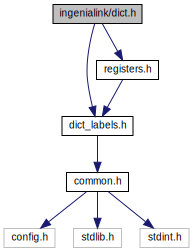
\includegraphics[width=265pt]{dict_8h__incl}
\end{center}
\end{figure}
This graph shows which files directly or indirectly include this file\+:\nopagebreak
\begin{figure}[H]
\begin{center}
\leavevmode
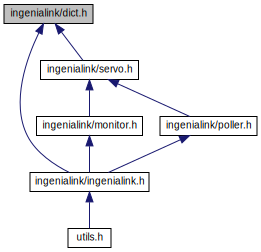
\includegraphics[width=333pt]{dict_8h__dep__incl}
\end{center}
\end{figure}
\subsection*{Typedefs}
\begin{DoxyCompactItemize}
\item 
typedef struct il\+\_\+dict \hyperlink{group__IL__DICT_gac2cb8ba7974d8506df3017879572fc84}{il\+\_\+dict\+\_\+t}
\begin{DoxyCompactList}\small\item\em Ingenia\+Link dictionary. \end{DoxyCompactList}\end{DoxyCompactItemize}
\subsection*{Functions}
\begin{DoxyCompactItemize}
\item 
\hyperlink{common_8h_a6bb629d26c52bfe10519ba3176853f47}{I\+L\+\_\+\+E\+X\+P\+O\+RT} \hyperlink{group__IL__DICT_gac2cb8ba7974d8506df3017879572fc84}{il\+\_\+dict\+\_\+t} $\ast$ \hyperlink{group__IL__DICT_gaf3d1da6ffb1d4efcf40946dc705230f2}{il\+\_\+dict\+\_\+create} (const char $\ast$dict\+\_\+f)
\begin{DoxyCompactList}\small\item\em Create a dictionary. \end{DoxyCompactList}\item 
\hyperlink{common_8h_a6bb629d26c52bfe10519ba3176853f47}{I\+L\+\_\+\+E\+X\+P\+O\+RT} void \hyperlink{group__IL__DICT_ga37cc4ceb38514581a5bbecb47f5cfa61}{il\+\_\+dict\+\_\+destroy} (\hyperlink{group__IL__DICT_gac2cb8ba7974d8506df3017879572fc84}{il\+\_\+dict\+\_\+t} $\ast$dict)
\begin{DoxyCompactList}\small\item\em Destroy a dictionary. \end{DoxyCompactList}\item 
\hyperlink{common_8h_a6bb629d26c52bfe10519ba3176853f47}{I\+L\+\_\+\+E\+X\+P\+O\+RT} int \hyperlink{group__IL__DICT_ga3ea660af3316835c1799ce8dca67b566}{il\+\_\+dict\+\_\+cat\+\_\+get} (\hyperlink{group__IL__DICT_gac2cb8ba7974d8506df3017879572fc84}{il\+\_\+dict\+\_\+t} $\ast$dict, const char $\ast$cat\+\_\+id, \hyperlink{group__IL__DICT__LABELS_ga69d1109256f465cbcfa8aac7fa592495}{il\+\_\+dict\+\_\+labels\+\_\+t} $\ast$$\ast$labels)
\begin{DoxyCompactList}\small\item\em Obtain category labels from ID. \end{DoxyCompactList}\item 
\hyperlink{common_8h_a6bb629d26c52bfe10519ba3176853f47}{I\+L\+\_\+\+E\+X\+P\+O\+RT} size\+\_\+t \hyperlink{group__IL__DICT_gac982efe51c1ceca824b89b729397bf6f}{il\+\_\+dict\+\_\+cat\+\_\+cnt} (\hyperlink{group__IL__DICT_gac2cb8ba7974d8506df3017879572fc84}{il\+\_\+dict\+\_\+t} $\ast$dict)
\begin{DoxyCompactList}\small\item\em Obtain number of categories in the dictionary. \end{DoxyCompactList}\item 
\hyperlink{common_8h_a6bb629d26c52bfe10519ba3176853f47}{I\+L\+\_\+\+E\+X\+P\+O\+RT} const char $\ast$$\ast$ \hyperlink{group__IL__DICT_ga254bc46b2740b8291fd0061e47c28758}{il\+\_\+dict\+\_\+cat\+\_\+ids\+\_\+get} (\hyperlink{group__IL__DICT_gac2cb8ba7974d8506df3017879572fc84}{il\+\_\+dict\+\_\+t} $\ast$dict)
\begin{DoxyCompactList}\small\item\em Obtain the list of category I\+Ds. \end{DoxyCompactList}\item 
\hyperlink{common_8h_a6bb629d26c52bfe10519ba3176853f47}{I\+L\+\_\+\+E\+X\+P\+O\+RT} void \hyperlink{group__IL__DICT_ga27125d99f6aa90dc36c3de0736993265}{il\+\_\+dict\+\_\+cat\+\_\+ids\+\_\+destroy} (const char $\ast$$\ast$cat\+\_\+ids)
\begin{DoxyCompactList}\small\item\em Destroy the list of obtained category I\+Ds. \end{DoxyCompactList}\item 
\hyperlink{common_8h_a6bb629d26c52bfe10519ba3176853f47}{I\+L\+\_\+\+E\+X\+P\+O\+RT} int \hyperlink{group__IL__DICT_ga79fb4bf5b1fab3d67a201c6e5b11e5e7}{il\+\_\+dict\+\_\+scat\+\_\+get} (\hyperlink{group__IL__DICT_gac2cb8ba7974d8506df3017879572fc84}{il\+\_\+dict\+\_\+t} $\ast$dict, const char $\ast$cat\+\_\+id, const char $\ast$scat\+\_\+id, \hyperlink{group__IL__DICT__LABELS_ga69d1109256f465cbcfa8aac7fa592495}{il\+\_\+dict\+\_\+labels\+\_\+t} $\ast$$\ast$labels)
\begin{DoxyCompactList}\small\item\em Obtain sub-\/category labels from a category. \end{DoxyCompactList}\item 
\hyperlink{common_8h_a6bb629d26c52bfe10519ba3176853f47}{I\+L\+\_\+\+E\+X\+P\+O\+RT} size\+\_\+t \hyperlink{group__IL__DICT_gac34ec4d95d8526d1cf09641c843ce7aa}{il\+\_\+dict\+\_\+scat\+\_\+cnt} (\hyperlink{group__IL__DICT_gac2cb8ba7974d8506df3017879572fc84}{il\+\_\+dict\+\_\+t} $\ast$dict, const char $\ast$cat\+\_\+id)
\begin{DoxyCompactList}\small\item\em Obtain number of sub-\/categories in a category. \end{DoxyCompactList}\item 
\hyperlink{common_8h_a6bb629d26c52bfe10519ba3176853f47}{I\+L\+\_\+\+E\+X\+P\+O\+RT} const char $\ast$$\ast$ \hyperlink{group__IL__DICT_ga51782d1acdcfd574ab717c6c721cb560}{il\+\_\+dict\+\_\+scat\+\_\+ids\+\_\+get} (\hyperlink{group__IL__DICT_gac2cb8ba7974d8506df3017879572fc84}{il\+\_\+dict\+\_\+t} $\ast$dict, const char $\ast$cat\+\_\+id)
\begin{DoxyCompactList}\small\item\em Obtain the list of category I\+Ds. \end{DoxyCompactList}\item 
\hyperlink{common_8h_a6bb629d26c52bfe10519ba3176853f47}{I\+L\+\_\+\+E\+X\+P\+O\+RT} void \hyperlink{group__IL__DICT_gaa558e902f07600780b351f9e58f443df}{il\+\_\+dict\+\_\+scat\+\_\+ids\+\_\+destroy} (const char $\ast$$\ast$scat\+\_\+ids)
\begin{DoxyCompactList}\small\item\em Destroy the list of obtained sub-\/category I\+Ds. \end{DoxyCompactList}\item 
\hyperlink{common_8h_a6bb629d26c52bfe10519ba3176853f47}{I\+L\+\_\+\+E\+X\+P\+O\+RT} int \hyperlink{group__IL__DICT_ga2c1e206d3c5d57a4a047855c2743fa5a}{il\+\_\+dict\+\_\+reg\+\_\+get} (\hyperlink{group__IL__DICT_gac2cb8ba7974d8506df3017879572fc84}{il\+\_\+dict\+\_\+t} $\ast$dict, const char $\ast$id, const \hyperlink{structil__reg__t}{il\+\_\+reg\+\_\+t} $\ast$$\ast$reg)
\begin{DoxyCompactList}\small\item\em Obtain register from ID. \end{DoxyCompactList}\item 
\hyperlink{common_8h_a6bb629d26c52bfe10519ba3176853f47}{I\+L\+\_\+\+E\+X\+P\+O\+RT} size\+\_\+t \hyperlink{group__IL__DICT_ga7d1b8cad25b75ec725c9dad237fe918a}{il\+\_\+dict\+\_\+reg\+\_\+cnt} (\hyperlink{group__IL__DICT_gac2cb8ba7974d8506df3017879572fc84}{il\+\_\+dict\+\_\+t} $\ast$dict)
\begin{DoxyCompactList}\small\item\em Obtain number of registers in the dictionary. \end{DoxyCompactList}\item 
\hyperlink{common_8h_a6bb629d26c52bfe10519ba3176853f47}{I\+L\+\_\+\+E\+X\+P\+O\+RT} const char $\ast$$\ast$ \hyperlink{group__IL__DICT_gaaf93ee11fe3006f72c03f03174abdf33}{il\+\_\+dict\+\_\+reg\+\_\+ids\+\_\+get} (\hyperlink{group__IL__DICT_gac2cb8ba7974d8506df3017879572fc84}{il\+\_\+dict\+\_\+t} $\ast$dict)
\begin{DoxyCompactList}\small\item\em Obtain the list of register I\+Ds. \end{DoxyCompactList}\item 
\hyperlink{common_8h_a6bb629d26c52bfe10519ba3176853f47}{I\+L\+\_\+\+E\+X\+P\+O\+RT} void \hyperlink{group__IL__DICT_gacd7922e14cb903f3342747ed21a00ec1}{il\+\_\+dict\+\_\+reg\+\_\+ids\+\_\+destroy} (const char $\ast$$\ast$regs)
\begin{DoxyCompactList}\small\item\em Destroy the list of obtained register I\+Ds. \end{DoxyCompactList}\end{DoxyCompactItemize}


\subsection{Detailed Description}
Dictionary. 


\hypertarget{dict__labels_8h}{}\section{ingenialink/dict\+\_\+labels.h File Reference}
\label{dict__labels_8h}\index{ingenialink/dict\+\_\+labels.\+h@{ingenialink/dict\+\_\+labels.\+h}}


Labels dictionary.  


{\ttfamily \#include \char`\"{}common.\+h\char`\"{}}\\*
Include dependency graph for dict\+\_\+labels.\+h\+:\nopagebreak
\begin{figure}[H]
\begin{center}
\leavevmode
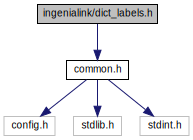
\includegraphics[width=265pt]{dict__labels_8h__incl}
\end{center}
\end{figure}
This graph shows which files directly or indirectly include this file\+:\nopagebreak
\begin{figure}[H]
\begin{center}
\leavevmode
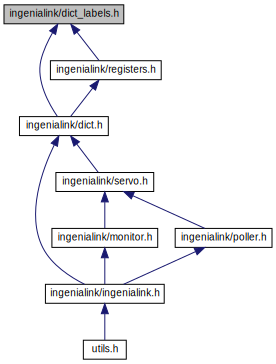
\includegraphics[width=349pt]{dict__labels_8h__dep__incl}
\end{center}
\end{figure}
\subsection*{Typedefs}
\begin{DoxyCompactItemize}
\item 
typedef struct il\+\_\+dict\+\_\+labels \hyperlink{group__IL__DICT__LABELS_ga69d1109256f465cbcfa8aac7fa592495}{il\+\_\+dict\+\_\+labels\+\_\+t}
\begin{DoxyCompactList}\small\item\em Labels dictionary. \end{DoxyCompactList}\end{DoxyCompactItemize}
\subsection*{Functions}
\begin{DoxyCompactItemize}
\item 
\hyperlink{common_8h_a6bb629d26c52bfe10519ba3176853f47}{I\+L\+\_\+\+E\+X\+P\+O\+RT} \hyperlink{group__IL__DICT__LABELS_ga69d1109256f465cbcfa8aac7fa592495}{il\+\_\+dict\+\_\+labels\+\_\+t} $\ast$ \hyperlink{group__IL__DICT__LABELS_ga3d1801f1328932552ae98c151079514b}{il\+\_\+dict\+\_\+labels\+\_\+create} (void)
\begin{DoxyCompactList}\small\item\em Create a labels dictionary. \end{DoxyCompactList}\item 
\hyperlink{common_8h_a6bb629d26c52bfe10519ba3176853f47}{I\+L\+\_\+\+E\+X\+P\+O\+RT} void \hyperlink{group__IL__DICT__LABELS_ga5dbfa1bafc6fd6e5c1e3356579e6b03a}{il\+\_\+dict\+\_\+labels\+\_\+destroy} (\hyperlink{group__IL__DICT__LABELS_ga69d1109256f465cbcfa8aac7fa592495}{il\+\_\+dict\+\_\+labels\+\_\+t} $\ast$labels)
\begin{DoxyCompactList}\small\item\em Destroy a labels dictionary. \end{DoxyCompactList}\item 
\hyperlink{common_8h_a6bb629d26c52bfe10519ba3176853f47}{I\+L\+\_\+\+E\+X\+P\+O\+RT} int \hyperlink{group__IL__DICT__LABELS_ga40033ee8b33c612a90feec8ecfeaec40}{il\+\_\+dict\+\_\+labels\+\_\+get} (\hyperlink{group__IL__DICT__LABELS_ga69d1109256f465cbcfa8aac7fa592495}{il\+\_\+dict\+\_\+labels\+\_\+t} $\ast$labels, const char $\ast$lang, const char $\ast$$\ast$label)
\begin{DoxyCompactList}\small\item\em Obtain the label given a language. \end{DoxyCompactList}\item 
\hyperlink{common_8h_a6bb629d26c52bfe10519ba3176853f47}{I\+L\+\_\+\+E\+X\+P\+O\+RT} void \hyperlink{group__IL__DICT__LABELS_ga31c468b558ffe84fbd413883ce80eb84}{il\+\_\+dict\+\_\+labels\+\_\+set} (\hyperlink{group__IL__DICT__LABELS_ga69d1109256f465cbcfa8aac7fa592495}{il\+\_\+dict\+\_\+labels\+\_\+t} $\ast$labels, const char $\ast$lang, const char $\ast$label)
\begin{DoxyCompactList}\small\item\em Set the label for a given language. \end{DoxyCompactList}\item 
\hyperlink{common_8h_a6bb629d26c52bfe10519ba3176853f47}{I\+L\+\_\+\+E\+X\+P\+O\+RT} void \hyperlink{group__IL__DICT__LABELS_ga8910c8ced7a73f8971264ae83208c07e}{il\+\_\+dict\+\_\+labels\+\_\+del} (\hyperlink{group__IL__DICT__LABELS_ga69d1109256f465cbcfa8aac7fa592495}{il\+\_\+dict\+\_\+labels\+\_\+t} $\ast$labels, const char $\ast$lang)
\begin{DoxyCompactList}\small\item\em Remove the label of the given language. \end{DoxyCompactList}\item 
\hyperlink{common_8h_a6bb629d26c52bfe10519ba3176853f47}{I\+L\+\_\+\+E\+X\+P\+O\+RT} size\+\_\+t \hyperlink{group__IL__DICT__LABELS_gae088f90ebbe304009129f502da289122}{il\+\_\+dict\+\_\+labels\+\_\+nlabels\+\_\+get} (\hyperlink{group__IL__DICT__LABELS_ga69d1109256f465cbcfa8aac7fa592495}{il\+\_\+dict\+\_\+labels\+\_\+t} $\ast$labels)
\begin{DoxyCompactList}\small\item\em Obtain the number of labels. \end{DoxyCompactList}\item 
\hyperlink{common_8h_a6bb629d26c52bfe10519ba3176853f47}{I\+L\+\_\+\+E\+X\+P\+O\+RT} const char $\ast$$\ast$ \hyperlink{group__IL__DICT__LABELS_ga8fe3b029fc05420611468de19d2b6439}{il\+\_\+dict\+\_\+labels\+\_\+langs\+\_\+get} (\hyperlink{group__IL__DICT__LABELS_ga69d1109256f465cbcfa8aac7fa592495}{il\+\_\+dict\+\_\+labels\+\_\+t} $\ast$labels)
\begin{DoxyCompactList}\small\item\em Obtain the languages available in the labels dictionary. \end{DoxyCompactList}\item 
\hyperlink{common_8h_a6bb629d26c52bfe10519ba3176853f47}{I\+L\+\_\+\+E\+X\+P\+O\+RT} void \hyperlink{group__IL__DICT__LABELS_ga522d5f9739e165588a79e085d9112f06}{il\+\_\+dict\+\_\+labels\+\_\+langs\+\_\+destroy} (const char $\ast$$\ast$langs)
\begin{DoxyCompactList}\small\item\em Destroy a list of languages. \end{DoxyCompactList}\end{DoxyCompactItemize}


\subsection{Detailed Description}
Labels dictionary. 


\hypertarget{err_8h}{}\section{ingenialink/err.h File Reference}
\label{err_8h}\index{ingenialink/err.\+h@{ingenialink/err.\+h}}


Error reporting.  


{\ttfamily \#include \char`\"{}common.\+h\char`\"{}}\\*
Include dependency graph for err.\+h\+:\nopagebreak
\begin{figure}[H]
\begin{center}
\leavevmode
\includegraphics[width=265pt]{err_8h__incl}
\end{center}
\end{figure}
This graph shows which files directly or indirectly include this file\+:\nopagebreak
\begin{figure}[H]
\begin{center}
\leavevmode
\includegraphics[width=199pt]{err_8h__dep__incl}
\end{center}
\end{figure}
\subsection*{Macros}
\begin{DoxyCompactItemize}
\item 
\#define \hyperlink{group__IL__ERR_ga19bb985b7d18cefc5aed42f9907fb2e0}{I\+L\+\_\+\+E\+F\+A\+IL}~-\/1
\begin{DoxyCompactList}\small\item\em General failure. \end{DoxyCompactList}\item 
\#define \hyperlink{group__IL__ERR_ga47cf82d575e6ab2f1af332b192f5a152}{I\+L\+\_\+\+E\+I\+N\+V\+AL}~-\/2
\begin{DoxyCompactList}\small\item\em Invalid values. \end{DoxyCompactList}\item 
\#define \hyperlink{group__IL__ERR_gac51a50be89cb8812586de3d7c403a3d2}{I\+L\+\_\+\+E\+T\+I\+M\+E\+D\+O\+UT}~-\/3
\begin{DoxyCompactList}\small\item\em Operation timed out. \end{DoxyCompactList}\item 
\#define \hyperlink{group__IL__ERR_gaf70f61bc8e6136b385edb92f72b0e676}{I\+L\+\_\+\+E\+N\+O\+M\+EM}~-\/4
\begin{DoxyCompactList}\small\item\em Not enough memory. \end{DoxyCompactList}\item 
\#define \hyperlink{group__IL__ERR_ga6450573c3dc43ce215afa857082692eb}{I\+L\+\_\+\+E\+A\+L\+R\+E\+A\+DY}~-\/5
\begin{DoxyCompactList}\small\item\em Already initialized. \end{DoxyCompactList}\item 
\#define \hyperlink{group__IL__ERR_ga09294945616872dde2c5ed98e257406d}{I\+L\+\_\+\+E\+D\+I\+S\+C\+O\+NN}~-\/6
\begin{DoxyCompactList}\small\item\em Device disconnected. \end{DoxyCompactList}\item 
\#define \hyperlink{group__IL__ERR_gaf8957a58cdc74c6cda94eb5bb990a26b}{I\+L\+\_\+\+E\+A\+C\+C\+E\+SS}~-\/7
\begin{DoxyCompactList}\small\item\em Access error. \end{DoxyCompactList}\item 
\#define \hyperlink{group__IL__ERR_ga85eb5ca72fd69575a0d927efcdd44188}{I\+L\+\_\+\+E\+S\+T\+A\+TE}~-\/8
\begin{DoxyCompactList}\small\item\em State error. \end{DoxyCompactList}\item 
\#define \hyperlink{group__IL__ERR_ga150b9efcf3d35150433b151f1f134b98}{I\+L\+\_\+\+E\+IO}~-\/9
\begin{DoxyCompactList}\small\item\em I/O error. \end{DoxyCompactList}\item 
\#define \hyperlink{group__IL__ERR_gacafae18e9ab826ace3f9135d2ed7deeb}{I\+L\+\_\+\+E\+N\+O\+T\+S\+UP}~-\/10
\begin{DoxyCompactList}\small\item\em Not supported. \end{DoxyCompactList}\end{DoxyCompactItemize}
\subsection*{Functions}
\begin{DoxyCompactItemize}
\item 
\hyperlink{common_8h_a6bb629d26c52bfe10519ba3176853f47}{I\+L\+\_\+\+E\+X\+P\+O\+RT} const char $\ast$ \hyperlink{group__IL__ERR_gac427087bdfe4aae17ff3e74de51cfe87}{ilerr\+\_\+last} (void)
\begin{DoxyCompactList}\small\item\em Obtain library last error details. \end{DoxyCompactList}\end{DoxyCompactItemize}


\subsection{Detailed Description}
Error reporting. 


\hypertarget{ingenialink_8h}{}\section{ingenialink/ingenialink.h File Reference}
\label{ingenialink_8h}\index{ingenialink/ingenialink.\+h@{ingenialink/ingenialink.\+h}}


Ingenia\+Link main header.  


{\ttfamily \#include \char`\"{}const.\+h\char`\"{}}\\*
{\ttfamily \#include \char`\"{}dict.\+h\char`\"{}}\\*
{\ttfamily \#include \char`\"{}err.\+h\char`\"{}}\\*
{\ttfamily \#include \char`\"{}monitor.\+h\char`\"{}}\\*
{\ttfamily \#include \char`\"{}poller.\+h\char`\"{}}\\*
{\ttfamily \#include \char`\"{}version.\+h\char`\"{}}\\*
Include dependency graph for ingenialink.\+h\+:\nopagebreak
\begin{figure}[H]
\begin{center}
\leavevmode
\includegraphics[width=350pt]{ingenialink_8h__incl}
\end{center}
\end{figure}
This graph shows which files directly or indirectly include this file\+:\nopagebreak
\begin{figure}[H]
\begin{center}
\leavevmode
\includegraphics[width=199pt]{ingenialink_8h__dep__incl}
\end{center}
\end{figure}


\subsection{Detailed Description}
Ingenia\+Link main header. 


\hypertarget{monitor_8h}{}\section{ingenialink/monitor.h File Reference}
\label{monitor_8h}\index{ingenialink/monitor.\+h@{ingenialink/monitor.\+h}}


Monitor.  


{\ttfamily \#include \char`\"{}servo.\+h\char`\"{}}\\*
Include dependency graph for monitor.\+h\+:\nopagebreak
\begin{figure}[H]
\begin{center}
\leavevmode
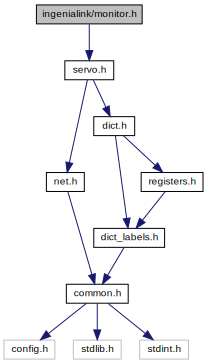
\includegraphics[width=280pt]{monitor_8h__incl}
\end{center}
\end{figure}
This graph shows which files directly or indirectly include this file\+:\nopagebreak
\begin{figure}[H]
\begin{center}
\leavevmode
\includegraphics[width=199pt]{monitor_8h__dep__incl}
\end{center}
\end{figure}
\subsection*{Data Structures}
\begin{DoxyCompactItemize}
\item 
struct \hyperlink{structil__monitor__acq__t}{il\+\_\+monitor\+\_\+acq\+\_\+t}
\begin{DoxyCompactList}\small\item\em Monitor acquisition results. \end{DoxyCompactList}\end{DoxyCompactItemize}
\subsection*{Macros}
\begin{DoxyCompactItemize}
\item 
\#define \hyperlink{group__IL__MONITOR_ga05007f227fb5f253ed8ba714c0efb2cd}{I\+L\+\_\+\+M\+O\+N\+I\+T\+O\+R\+\_\+\+C\+H\+\_\+\+N\+UM}~4
\begin{DoxyCompactList}\small\item\em Number of channels. \end{DoxyCompactList}\end{DoxyCompactItemize}
\subsection*{Typedefs}
\begin{DoxyCompactItemize}
\item 
typedef struct il\+\_\+monitor \hyperlink{group__IL__MONITOR_ga40e12e851c8c83202f0bccbaaafbc1f3}{il\+\_\+monitor\+\_\+t}
\begin{DoxyCompactList}\small\item\em Ingenia\+Link monitor. \end{DoxyCompactList}\end{DoxyCompactItemize}
\subsection*{Enumerations}
\begin{DoxyCompactItemize}
\item 
enum \hyperlink{group__IL__MONITOR_ga713d0c15082ee67cb77d384d4537e107}{il\+\_\+monitor\+\_\+trigger\+\_\+t} \{ \\*
\hyperlink{group__IL__MONITOR_gga713d0c15082ee67cb77d384d4537e107a7a2adbfffa9d5301d44c58aee1524947}{I\+L\+\_\+\+M\+O\+N\+I\+T\+O\+R\+\_\+\+T\+R\+I\+G\+G\+E\+R\+\_\+\+I\+M\+M\+E\+D\+I\+A\+TE} = 0, 
\hyperlink{group__IL__MONITOR_gga713d0c15082ee67cb77d384d4537e107a3d9776dc06a1769bb3bac474d0d2f671}{I\+L\+\_\+\+M\+O\+N\+I\+T\+O\+R\+\_\+\+T\+R\+I\+G\+G\+E\+R\+\_\+\+M\+O\+T\+I\+ON} = 1, 
\hyperlink{group__IL__MONITOR_gga713d0c15082ee67cb77d384d4537e107a3e127c86c21f607d0df72b64403adb42}{I\+L\+\_\+\+M\+O\+N\+I\+T\+O\+R\+\_\+\+T\+R\+I\+G\+G\+E\+R\+\_\+\+P\+OS} = 2, 
\hyperlink{group__IL__MONITOR_gga713d0c15082ee67cb77d384d4537e107afff4584d639834baa2242e2ab08aafd6}{I\+L\+\_\+\+M\+O\+N\+I\+T\+O\+R\+\_\+\+T\+R\+I\+G\+G\+E\+R\+\_\+\+N\+EG} = 3, 
\\*
\hyperlink{group__IL__MONITOR_gga713d0c15082ee67cb77d384d4537e107af66901be0c630d815042a98f13b0781b}{I\+L\+\_\+\+M\+O\+N\+I\+T\+O\+R\+\_\+\+T\+R\+I\+G\+G\+E\+R\+\_\+\+W\+I\+N\+D\+OW} = 4, 
\hyperlink{group__IL__MONITOR_gga713d0c15082ee67cb77d384d4537e107aededed6d0aa1e43dd19b0019f857db06}{I\+L\+\_\+\+M\+O\+N\+I\+T\+O\+R\+\_\+\+T\+R\+I\+G\+G\+E\+R\+\_\+\+D\+IN} = 5
 \}\begin{DoxyCompactList}\small\item\em Trigger modes. \end{DoxyCompactList}
\end{DoxyCompactItemize}
\subsection*{Functions}
\begin{DoxyCompactItemize}
\item 
\hyperlink{common_8h_a6bb629d26c52bfe10519ba3176853f47}{I\+L\+\_\+\+E\+X\+P\+O\+RT} \hyperlink{group__IL__MONITOR_ga40e12e851c8c83202f0bccbaaafbc1f3}{il\+\_\+monitor\+\_\+t} $\ast$ \hyperlink{group__IL__MONITOR_gabab1b2d47a46eeabfcaa9ec5ce7c49a8}{il\+\_\+monitor\+\_\+create} (\hyperlink{group__IL__SERVO_ga3369ddfcc33492fe3a28f96cf455b13e}{il\+\_\+servo\+\_\+t} $\ast$servo)
\begin{DoxyCompactList}\small\item\em Create monitor instance. \end{DoxyCompactList}\item 
\hyperlink{common_8h_a6bb629d26c52bfe10519ba3176853f47}{I\+L\+\_\+\+E\+X\+P\+O\+RT} void \hyperlink{group__IL__MONITOR_ga3bc1e187d696eadd07a3f33b502c998a}{il\+\_\+monitor\+\_\+destroy} (\hyperlink{group__IL__MONITOR_ga40e12e851c8c83202f0bccbaaafbc1f3}{il\+\_\+monitor\+\_\+t} $\ast$monitor)
\begin{DoxyCompactList}\small\item\em Destroy a monitor instance. \end{DoxyCompactList}\item 
\hyperlink{common_8h_a6bb629d26c52bfe10519ba3176853f47}{I\+L\+\_\+\+E\+X\+P\+O\+RT} int \hyperlink{group__IL__MONITOR_ga41ec8c974f4322537d714844be7b8a2a}{il\+\_\+monitor\+\_\+start} (\hyperlink{group__IL__MONITOR_ga40e12e851c8c83202f0bccbaaafbc1f3}{il\+\_\+monitor\+\_\+t} $\ast$monitor)
\begin{DoxyCompactList}\small\item\em Start monitor. \end{DoxyCompactList}\item 
\hyperlink{common_8h_a6bb629d26c52bfe10519ba3176853f47}{I\+L\+\_\+\+E\+X\+P\+O\+RT} void \hyperlink{group__IL__MONITOR_ga2408490312f9562407f93111a4deece8}{il\+\_\+monitor\+\_\+stop} (\hyperlink{group__IL__MONITOR_ga40e12e851c8c83202f0bccbaaafbc1f3}{il\+\_\+monitor\+\_\+t} $\ast$monitor)
\begin{DoxyCompactList}\small\item\em Stop monitor. \end{DoxyCompactList}\item 
\hyperlink{common_8h_a6bb629d26c52bfe10519ba3176853f47}{I\+L\+\_\+\+E\+X\+P\+O\+RT} int \hyperlink{group__IL__MONITOR_ga5a2bfd4b0f37f4abee986a77afae5b32}{il\+\_\+monitor\+\_\+wait} (\hyperlink{group__IL__MONITOR_ga40e12e851c8c83202f0bccbaaafbc1f3}{il\+\_\+monitor\+\_\+t} $\ast$monitor, int timeout)
\begin{DoxyCompactList}\small\item\em Wait until current acquisition is completed. \end{DoxyCompactList}\item 
\hyperlink{common_8h_a6bb629d26c52bfe10519ba3176853f47}{I\+L\+\_\+\+E\+X\+P\+O\+RT} void \hyperlink{group__IL__MONITOR_gad6231f5d154969361fdd05d3f84707bb}{il\+\_\+monitor\+\_\+data\+\_\+get} (\hyperlink{group__IL__MONITOR_ga40e12e851c8c83202f0bccbaaafbc1f3}{il\+\_\+monitor\+\_\+t} $\ast$monitor, \hyperlink{structil__monitor__acq__t}{il\+\_\+monitor\+\_\+acq\+\_\+t} $\ast$$\ast$acq)
\begin{DoxyCompactList}\small\item\em Obtain current available data. \end{DoxyCompactList}\item 
\hyperlink{common_8h_a6bb629d26c52bfe10519ba3176853f47}{I\+L\+\_\+\+E\+X\+P\+O\+RT} int \hyperlink{group__IL__MONITOR_ga8fc675f7d849ebcf162e396a98b6c710}{il\+\_\+monitor\+\_\+configure} (\hyperlink{group__IL__MONITOR_ga40e12e851c8c83202f0bccbaaafbc1f3}{il\+\_\+monitor\+\_\+t} $\ast$monitor, unsigned int t\+\_\+s, size\+\_\+t delay\+\_\+samples, size\+\_\+t max\+\_\+samples)
\begin{DoxyCompactList}\small\item\em Configure monitor parameters. \end{DoxyCompactList}\item 
\hyperlink{common_8h_a6bb629d26c52bfe10519ba3176853f47}{I\+L\+\_\+\+E\+X\+P\+O\+RT} int \hyperlink{group__IL__MONITOR_gacda4fa0bc57e96988e62f895b256a62a}{il\+\_\+monitor\+\_\+ch\+\_\+configure} (\hyperlink{group__IL__MONITOR_ga40e12e851c8c83202f0bccbaaafbc1f3}{il\+\_\+monitor\+\_\+t} $\ast$monitor, int ch, const \hyperlink{structil__reg__t}{il\+\_\+reg\+\_\+t} $\ast$reg, const char $\ast$id)
\begin{DoxyCompactList}\small\item\em Configure channel mapping. \end{DoxyCompactList}\item 
\hyperlink{common_8h_a6bb629d26c52bfe10519ba3176853f47}{I\+L\+\_\+\+E\+X\+P\+O\+RT} int \hyperlink{group__IL__MONITOR_ga33dffe1563b9d4a53d7623a123d7710c}{il\+\_\+monitor\+\_\+ch\+\_\+disable} (\hyperlink{group__IL__MONITOR_ga40e12e851c8c83202f0bccbaaafbc1f3}{il\+\_\+monitor\+\_\+t} $\ast$monitor, int ch)
\begin{DoxyCompactList}\small\item\em Disable one channel. \end{DoxyCompactList}\item 
\hyperlink{common_8h_a6bb629d26c52bfe10519ba3176853f47}{I\+L\+\_\+\+E\+X\+P\+O\+RT} int \hyperlink{group__IL__MONITOR_ga19230bb2f539a808deb9e42afcb58678}{il\+\_\+monitor\+\_\+ch\+\_\+disable\+\_\+all} (\hyperlink{group__IL__MONITOR_ga40e12e851c8c83202f0bccbaaafbc1f3}{il\+\_\+monitor\+\_\+t} $\ast$monitor)
\begin{DoxyCompactList}\small\item\em Disable all channels. \end{DoxyCompactList}\item 
\hyperlink{common_8h_a6bb629d26c52bfe10519ba3176853f47}{I\+L\+\_\+\+E\+X\+P\+O\+RT} int \hyperlink{group__IL__MONITOR_ga98522072a54d7e70fe94409d666d58cd}{il\+\_\+monitor\+\_\+trigger\+\_\+configure} (\hyperlink{group__IL__MONITOR_ga40e12e851c8c83202f0bccbaaafbc1f3}{il\+\_\+monitor\+\_\+t} $\ast$monitor, \hyperlink{group__IL__MONITOR_ga713d0c15082ee67cb77d384d4537e107}{il\+\_\+monitor\+\_\+trigger\+\_\+t} mode, size\+\_\+t delay\+\_\+samples, const \hyperlink{structil__reg__t}{il\+\_\+reg\+\_\+t} $\ast$source, const char $\ast$source\+\_\+id, double th\+\_\+pos, double th\+\_\+neg, uint32\+\_\+t din\+\_\+msk)
\begin{DoxyCompactList}\small\item\em Trigger configuration. \end{DoxyCompactList}\end{DoxyCompactItemize}


\subsection{Detailed Description}
Monitor. 


\hypertarget{net_8h}{}\section{ingenialink/net.h File Reference}
\label{net_8h}\index{ingenialink/net.\+h@{ingenialink/net.\+h}}


Network.  


{\ttfamily \#include \char`\"{}common.\+h\char`\"{}}\\*
Include dependency graph for net.\+h\+:\nopagebreak
\begin{figure}[H]
\begin{center}
\leavevmode
\includegraphics[width=265pt]{net_8h__incl}
\end{center}
\end{figure}
This graph shows which files directly or indirectly include this file\+:\nopagebreak
\begin{figure}[H]
\begin{center}
\leavevmode
\includegraphics[width=301pt]{net_8h__dep__incl}
\end{center}
\end{figure}
\subsection*{Data Structures}
\begin{DoxyCompactItemize}
\item 
struct \hyperlink{structil__net__opts__t}{il\+\_\+net\+\_\+opts\+\_\+t}
\begin{DoxyCompactList}\small\item\em Network initialization options. \end{DoxyCompactList}\item 
struct \hyperlink{structil__net__dev__list}{il\+\_\+net\+\_\+dev\+\_\+list}
\begin{DoxyCompactList}\small\item\em network devices list. \end{DoxyCompactList}\item 
struct \hyperlink{structil__net__servos__list}{il\+\_\+net\+\_\+servos\+\_\+list}
\begin{DoxyCompactList}\small\item\em Network servos list. \end{DoxyCompactList}\end{DoxyCompactItemize}
\subsection*{Macros}
\begin{DoxyCompactItemize}
\item 
\#define \hyperlink{group__IL__NET_ga7fb88a9dcbf2c6ae143dc9d16c70ad4f}{I\+L\+\_\+\+N\+E\+T\+\_\+\+T\+I\+M\+E\+O\+U\+T\+\_\+\+R\+D\+\_\+\+D\+EF}~500
\begin{DoxyCompactList}\small\item\em Default read timeout (ms). \end{DoxyCompactList}\item 
\#define \hyperlink{group__IL__NET_gaf43b0714cfed3be5907c593e18d4481d}{I\+L\+\_\+\+N\+E\+T\+\_\+\+T\+I\+M\+E\+O\+U\+T\+\_\+\+W\+R\+\_\+\+D\+EF}~500
\begin{DoxyCompactList}\small\item\em Default write timeout (ms). \end{DoxyCompactList}\item 
\#define \hyperlink{group__IL__NET_ga9c33d1c3bf660e4cb980a9e7a676cb88}{I\+L\+\_\+\+N\+E\+T\+\_\+\+P\+O\+R\+T\+\_\+\+SZ}~128U
\begin{DoxyCompactList}\small\item\em Port maximum size. \end{DoxyCompactList}\item 
\#define \hyperlink{group__IL__NET_ga70cbad080864d1cc39dd701f9a27d9b6}{il\+\_\+net\+\_\+servos\+\_\+list\+\_\+foreach}(item,  lst)~for ((item) = (lst); (item); (item) = (item)-\/$>$next)
\begin{DoxyCompactList}\small\item\em Utility macro to iterate over a list of network servos list. \end{DoxyCompactList}\item 
\#define \hyperlink{group__IL__NET_gae80aefde62011dd14dbf60840669cc54}{il\+\_\+net\+\_\+dev\+\_\+list\+\_\+foreach}(item,  lst)~for ((item) = (lst); (item); (item) = (item)-\/$>$next)
\begin{DoxyCompactList}\small\item\em Utility macro to iterate over a list of network devices. \end{DoxyCompactList}\end{DoxyCompactItemize}
\subsection*{Typedefs}
\begin{DoxyCompactItemize}
\item 
typedef struct il\+\_\+net \hyperlink{group__IL__NET_ga0657204ab779a5b7a504aa0b895d1ae6}{il\+\_\+net\+\_\+t}
\begin{DoxyCompactList}\small\item\em Network. \end{DoxyCompactList}\item 
typedef struct \hyperlink{structil__net__dev__list}{il\+\_\+net\+\_\+dev\+\_\+list} \hyperlink{group__IL__NET_ga9c0173ee0e17218e9f6dcc5ae0a6f74d}{il\+\_\+net\+\_\+dev\+\_\+list\+\_\+t}
\begin{DoxyCompactList}\small\item\em network devices list. \end{DoxyCompactList}\item 
typedef struct \hyperlink{structil__net__servos__list}{il\+\_\+net\+\_\+servos\+\_\+list} \hyperlink{group__IL__NET_ga81660630b147245b0a160f13ef465811}{il\+\_\+net\+\_\+servos\+\_\+list\+\_\+t}
\begin{DoxyCompactList}\small\item\em Network servos list. \end{DoxyCompactList}\item 
typedef void($\ast$ \hyperlink{group__IL__NET_ga4ba09545bd04fa6df4f0a26f14df84f7}{il\+\_\+net\+\_\+servos\+\_\+on\+\_\+found\+\_\+t}) (void $\ast$ctx, uint8\+\_\+t id)
\begin{DoxyCompactList}\small\item\em Node found callback. \end{DoxyCompactList}\item 
typedef struct il\+\_\+net\+\_\+dev\+\_\+mon \hyperlink{group__IL__NET_ga732e586d3465268782c0c227056736e5}{il\+\_\+net\+\_\+dev\+\_\+mon\+\_\+t}
\begin{DoxyCompactList}\small\item\em Network device monitor. \end{DoxyCompactList}\item 
typedef void($\ast$ \hyperlink{group__IL__NET_ga86bfa409239ad771481bd4dd1a451367}{il\+\_\+net\+\_\+dev\+\_\+on\+\_\+evt\+\_\+t}) (void $\ast$ctx, \hyperlink{group__IL__NET_ga6e78452befa7532716d8035eb293bc10}{il\+\_\+net\+\_\+dev\+\_\+evt\+\_\+t} evt, const char $\ast$port)
\begin{DoxyCompactList}\small\item\em Network device event callback. \end{DoxyCompactList}\end{DoxyCompactItemize}
\subsection*{Enumerations}
\begin{DoxyCompactItemize}
\item 
enum \hyperlink{group__IL__NET_ga9629f7451843e493e7665754b5c2feca}{il\+\_\+net\+\_\+prot\+\_\+t} \{ \hyperlink{group__IL__NET_gga9629f7451843e493e7665754b5c2fecaafb048fa22f8e422dd8af49370e5f24a5}{I\+L\+\_\+\+N\+E\+T\+\_\+\+P\+R\+O\+T\+\_\+\+E\+U\+SB}, 
\hyperlink{group__IL__NET_gga9629f7451843e493e7665754b5c2fecaacdfe55790a47d94d5e6a633598f4eb5c}{I\+L\+\_\+\+N\+E\+T\+\_\+\+P\+R\+O\+T\+\_\+\+M\+CB}
 \}\begin{DoxyCompactList}\small\item\em Network protocols. \end{DoxyCompactList}
\item 
enum \hyperlink{group__IL__NET_ga0391fec0328dc9cfd7b91990998930a7}{il\+\_\+net\+\_\+state\+\_\+t} \{ \hyperlink{group__IL__NET_gga0391fec0328dc9cfd7b91990998930a7a2e3dc49a7ff84f0bae3fc4a237d63fc5}{I\+L\+\_\+\+N\+E\+T\+\_\+\+S\+T\+A\+T\+E\+\_\+\+C\+O\+N\+N\+E\+C\+T\+ED}, 
\hyperlink{group__IL__NET_gga0391fec0328dc9cfd7b91990998930a7abf97cabc9736acafc52a079fe3a98a6f}{I\+L\+\_\+\+N\+E\+T\+\_\+\+S\+T\+A\+T\+E\+\_\+\+D\+I\+S\+C\+O\+N\+N\+E\+C\+T\+ED}, 
\hyperlink{group__IL__NET_gga0391fec0328dc9cfd7b91990998930a7ad761916bd5ecfefe4578e53c39bf8ade}{I\+L\+\_\+\+N\+E\+T\+\_\+\+S\+T\+A\+T\+E\+\_\+\+F\+A\+U\+L\+TY}
 \}\begin{DoxyCompactList}\small\item\em Network state. \end{DoxyCompactList}
\item 
enum \hyperlink{group__IL__NET_ga6e78452befa7532716d8035eb293bc10}{il\+\_\+net\+\_\+dev\+\_\+evt\+\_\+t} \{ \hyperlink{group__IL__NET_gga6e78452befa7532716d8035eb293bc10a643a98c3c2f49473604cdda65b612103}{I\+L\+\_\+\+N\+E\+T\+\_\+\+D\+E\+V\+\_\+\+E\+V\+T\+\_\+\+A\+D\+D\+ED}, 
\hyperlink{group__IL__NET_gga6e78452befa7532716d8035eb293bc10a49f0b316d9ca1d19fa3b31cba22e8581}{I\+L\+\_\+\+N\+E\+T\+\_\+\+D\+E\+V\+\_\+\+E\+V\+T\+\_\+\+R\+E\+M\+O\+V\+ED}
 \}\begin{DoxyCompactList}\small\item\em Device monitor event types. \end{DoxyCompactList}
\end{DoxyCompactItemize}
\subsection*{Functions}
\begin{DoxyCompactItemize}
\item 
\hyperlink{common_8h_a6bb629d26c52bfe10519ba3176853f47}{I\+L\+\_\+\+E\+X\+P\+O\+RT} \hyperlink{group__IL__NET_ga0657204ab779a5b7a504aa0b895d1ae6}{il\+\_\+net\+\_\+t} $\ast$ \hyperlink{group__IL__NET_gaed82d6f49871934f3b6fdf3a9a022cc6}{il\+\_\+net\+\_\+create} (\hyperlink{group__IL__NET_ga9629f7451843e493e7665754b5c2feca}{il\+\_\+net\+\_\+prot\+\_\+t} prot, const \hyperlink{structil__net__opts__t}{il\+\_\+net\+\_\+opts\+\_\+t} $\ast$opts)
\begin{DoxyCompactList}\small\item\em Create a network. \end{DoxyCompactList}\item 
\hyperlink{common_8h_a6bb629d26c52bfe10519ba3176853f47}{I\+L\+\_\+\+E\+X\+P\+O\+RT} void \hyperlink{group__IL__NET_ga4b9335320c644d86491b3bc20e055f5f}{il\+\_\+net\+\_\+destroy} (\hyperlink{group__IL__NET_ga0657204ab779a5b7a504aa0b895d1ae6}{il\+\_\+net\+\_\+t} $\ast$net)
\begin{DoxyCompactList}\small\item\em Destroy a network. \end{DoxyCompactList}\item 
\hyperlink{common_8h_a6bb629d26c52bfe10519ba3176853f47}{I\+L\+\_\+\+E\+X\+P\+O\+RT} int \hyperlink{group__IL__NET_gae7992a1213d501e4df7ef3ae64e0c835}{il\+\_\+net\+\_\+connect} (\hyperlink{group__IL__NET_ga0657204ab779a5b7a504aa0b895d1ae6}{il\+\_\+net\+\_\+t} $\ast$net)
\begin{DoxyCompactList}\small\item\em Connect network. \end{DoxyCompactList}\item 
\hyperlink{common_8h_a6bb629d26c52bfe10519ba3176853f47}{I\+L\+\_\+\+E\+X\+P\+O\+RT} void \hyperlink{group__IL__NET_gaaacc31d9cbf294a17dae29eacfb7e735}{il\+\_\+net\+\_\+disconnect} (\hyperlink{group__IL__NET_ga0657204ab779a5b7a504aa0b895d1ae6}{il\+\_\+net\+\_\+t} $\ast$net)
\begin{DoxyCompactList}\small\item\em Disconnect network. \end{DoxyCompactList}\item 
\hyperlink{common_8h_a6bb629d26c52bfe10519ba3176853f47}{I\+L\+\_\+\+E\+X\+P\+O\+RT} \hyperlink{group__IL__NET_ga9629f7451843e493e7665754b5c2feca}{il\+\_\+net\+\_\+prot\+\_\+t} \hyperlink{group__IL__NET_gaa72feed444ad53acc497505239b950f9}{il\+\_\+net\+\_\+prot\+\_\+get} (\hyperlink{group__IL__NET_ga0657204ab779a5b7a504aa0b895d1ae6}{il\+\_\+net\+\_\+t} $\ast$net)
\begin{DoxyCompactList}\small\item\em Obtain network protocol. \end{DoxyCompactList}\item 
\hyperlink{common_8h_a6bb629d26c52bfe10519ba3176853f47}{I\+L\+\_\+\+E\+X\+P\+O\+RT} \hyperlink{group__IL__NET_ga0391fec0328dc9cfd7b91990998930a7}{il\+\_\+net\+\_\+state\+\_\+t} \hyperlink{group__IL__NET_ga83bb157bace16b18f1ebba59a6c6fe59}{il\+\_\+net\+\_\+state\+\_\+get} (\hyperlink{group__IL__NET_ga0657204ab779a5b7a504aa0b895d1ae6}{il\+\_\+net\+\_\+t} $\ast$net)
\begin{DoxyCompactList}\small\item\em Obtain network state. \end{DoxyCompactList}\item 
\hyperlink{common_8h_a6bb629d26c52bfe10519ba3176853f47}{I\+L\+\_\+\+E\+X\+P\+O\+RT} const char $\ast$ \hyperlink{group__IL__NET_ga307f630cca0e1d5e1ff44ce04abc9389}{il\+\_\+net\+\_\+port\+\_\+get} (\hyperlink{group__IL__NET_ga0657204ab779a5b7a504aa0b895d1ae6}{il\+\_\+net\+\_\+t} $\ast$net)
\begin{DoxyCompactList}\small\item\em Obtain network port. \end{DoxyCompactList}\item 
\hyperlink{common_8h_a6bb629d26c52bfe10519ba3176853f47}{I\+L\+\_\+\+E\+X\+P\+O\+RT} \hyperlink{group__IL__NET_ga81660630b147245b0a160f13ef465811}{il\+\_\+net\+\_\+servos\+\_\+list\+\_\+t} $\ast$ \hyperlink{group__IL__NET_ga6167fb50406d818120a069b681d377df}{il\+\_\+net\+\_\+servos\+\_\+list\+\_\+get} (\hyperlink{group__IL__NET_ga0657204ab779a5b7a504aa0b895d1ae6}{il\+\_\+net\+\_\+t} $\ast$net, \hyperlink{group__IL__NET_ga4ba09545bd04fa6df4f0a26f14df84f7}{il\+\_\+net\+\_\+servos\+\_\+on\+\_\+found\+\_\+t} on\+\_\+found, void $\ast$ctx)
\begin{DoxyCompactList}\small\item\em Obtain network servos list. \end{DoxyCompactList}\item 
\hyperlink{common_8h_a6bb629d26c52bfe10519ba3176853f47}{I\+L\+\_\+\+E\+X\+P\+O\+RT} void \hyperlink{group__IL__NET_ga7bb08347585c3760ba2f0c471c478d12}{il\+\_\+net\+\_\+servos\+\_\+list\+\_\+destroy} (\hyperlink{group__IL__NET_ga81660630b147245b0a160f13ef465811}{il\+\_\+net\+\_\+servos\+\_\+list\+\_\+t} $\ast$lst)
\begin{DoxyCompactList}\small\item\em Destroy network servos list. \end{DoxyCompactList}\item 
\hyperlink{common_8h_a6bb629d26c52bfe10519ba3176853f47}{I\+L\+\_\+\+E\+X\+P\+O\+RT} \hyperlink{group__IL__NET_ga732e586d3465268782c0c227056736e5}{il\+\_\+net\+\_\+dev\+\_\+mon\+\_\+t} $\ast$ \hyperlink{group__IL__NET_ga78022aea4dc9147a87544533f2999bd9}{il\+\_\+net\+\_\+dev\+\_\+mon\+\_\+create} (\hyperlink{group__IL__NET_ga9629f7451843e493e7665754b5c2feca}{il\+\_\+net\+\_\+prot\+\_\+t} prot)
\begin{DoxyCompactList}\small\item\em Create a network device monitor. \end{DoxyCompactList}\item 
\hyperlink{common_8h_a6bb629d26c52bfe10519ba3176853f47}{I\+L\+\_\+\+E\+X\+P\+O\+RT} int \hyperlink{group__IL__NET_gac0ed4c0656f51a2e691907ccd8ac94ce}{il\+\_\+net\+\_\+dev\+\_\+mon\+\_\+start} (\hyperlink{group__IL__NET_ga732e586d3465268782c0c227056736e5}{il\+\_\+net\+\_\+dev\+\_\+mon\+\_\+t} $\ast$mon, \hyperlink{group__IL__NET_ga86bfa409239ad771481bd4dd1a451367}{il\+\_\+net\+\_\+dev\+\_\+on\+\_\+evt\+\_\+t} on\+\_\+evt, void $\ast$ctx)
\begin{DoxyCompactList}\small\item\em Start the network device monitor. \end{DoxyCompactList}\item 
\hyperlink{common_8h_a6bb629d26c52bfe10519ba3176853f47}{I\+L\+\_\+\+E\+X\+P\+O\+RT} void \hyperlink{group__IL__NET_ga88fb38bdcb516562c504588b37ab934a}{il\+\_\+net\+\_\+dev\+\_\+mon\+\_\+stop} (\hyperlink{group__IL__NET_ga732e586d3465268782c0c227056736e5}{il\+\_\+net\+\_\+dev\+\_\+mon\+\_\+t} $\ast$mon)
\begin{DoxyCompactList}\small\item\em Stop the network device monitor. \end{DoxyCompactList}\item 
\hyperlink{common_8h_a6bb629d26c52bfe10519ba3176853f47}{I\+L\+\_\+\+E\+X\+P\+O\+RT} void \hyperlink{group__IL__NET_ga71f76ab3a41bde25b3b77a661ff767d8}{il\+\_\+net\+\_\+dev\+\_\+mon\+\_\+destroy} (\hyperlink{group__IL__NET_ga732e586d3465268782c0c227056736e5}{il\+\_\+net\+\_\+dev\+\_\+mon\+\_\+t} $\ast$mon)
\begin{DoxyCompactList}\small\item\em Destroy the network device monitor. \end{DoxyCompactList}\item 
\hyperlink{common_8h_a6bb629d26c52bfe10519ba3176853f47}{I\+L\+\_\+\+E\+X\+P\+O\+RT} \hyperlink{group__IL__NET_ga9c0173ee0e17218e9f6dcc5ae0a6f74d}{il\+\_\+net\+\_\+dev\+\_\+list\+\_\+t} $\ast$ \hyperlink{group__IL__NET_gaa59e20a4749f276763c45e5d278934d3}{il\+\_\+net\+\_\+dev\+\_\+list\+\_\+get} (\hyperlink{group__IL__NET_ga9629f7451843e493e7665754b5c2feca}{il\+\_\+net\+\_\+prot\+\_\+t} prot)
\begin{DoxyCompactList}\small\item\em Obtain network devices list. \end{DoxyCompactList}\item 
\hyperlink{common_8h_a6bb629d26c52bfe10519ba3176853f47}{I\+L\+\_\+\+E\+X\+P\+O\+RT} void \hyperlink{group__IL__NET_ga86d432b3a9ef2fdc6719e19a59dcbf65}{il\+\_\+net\+\_\+dev\+\_\+list\+\_\+destroy} (\hyperlink{group__IL__NET_ga9c0173ee0e17218e9f6dcc5ae0a6f74d}{il\+\_\+net\+\_\+dev\+\_\+list\+\_\+t} $\ast$lst)
\begin{DoxyCompactList}\small\item\em Destroy Network device list. \end{DoxyCompactList}\end{DoxyCompactItemize}


\subsection{Detailed Description}
Network. 


\hypertarget{poller_8h}{}\section{ingenialink/poller.h File Reference}
\label{poller_8h}\index{ingenialink/poller.\+h@{ingenialink/poller.\+h}}


Poller.  


{\ttfamily \#include \char`\"{}servo.\+h\char`\"{}}\\*
Include dependency graph for poller.\+h\+:\nopagebreak
\begin{figure}[H]
\begin{center}
\leavevmode
\includegraphics[width=280pt]{poller_8h__incl}
\end{center}
\end{figure}
This graph shows which files directly or indirectly include this file\+:\nopagebreak
\begin{figure}[H]
\begin{center}
\leavevmode
\includegraphics[width=199pt]{poller_8h__dep__incl}
\end{center}
\end{figure}
\subsection*{Data Structures}
\begin{DoxyCompactItemize}
\item 
struct \hyperlink{structil__poller__acq__t}{il\+\_\+poller\+\_\+acq\+\_\+t}
\begin{DoxyCompactList}\small\item\em Poller acquisition results. \end{DoxyCompactList}\end{DoxyCompactItemize}
\subsection*{Typedefs}
\begin{DoxyCompactItemize}
\item 
typedef struct il\+\_\+poller \hyperlink{group__IL__POLLER_ga896ad3836b2a1e121ce8b0c30c58d3ab}{il\+\_\+poller\+\_\+t}
\begin{DoxyCompactList}\small\item\em Ingenia\+Link poller. \end{DoxyCompactList}\end{DoxyCompactItemize}
\subsection*{Functions}
\begin{DoxyCompactItemize}
\item 
\hyperlink{common_8h_a6bb629d26c52bfe10519ba3176853f47}{I\+L\+\_\+\+E\+X\+P\+O\+RT} \hyperlink{group__IL__POLLER_ga896ad3836b2a1e121ce8b0c30c58d3ab}{il\+\_\+poller\+\_\+t} $\ast$ \hyperlink{group__IL__POLLER_gaf1a6d95123039ac685439062c34e7e54}{il\+\_\+poller\+\_\+create} (\hyperlink{group__IL__SERVO_ga3369ddfcc33492fe3a28f96cf455b13e}{il\+\_\+servo\+\_\+t} $\ast$servo, size\+\_\+t n\+\_\+ch)
\begin{DoxyCompactList}\small\item\em Create a register poller. \end{DoxyCompactList}\item 
\hyperlink{common_8h_a6bb629d26c52bfe10519ba3176853f47}{I\+L\+\_\+\+E\+X\+P\+O\+RT} void \hyperlink{group__IL__POLLER_gada8133cbba4d0212e6d5c84dab03d407}{il\+\_\+poller\+\_\+destroy} (\hyperlink{group__IL__POLLER_ga896ad3836b2a1e121ce8b0c30c58d3ab}{il\+\_\+poller\+\_\+t} $\ast$poller)
\begin{DoxyCompactList}\small\item\em Destroy a register poller. \end{DoxyCompactList}\item 
\hyperlink{common_8h_a6bb629d26c52bfe10519ba3176853f47}{I\+L\+\_\+\+E\+X\+P\+O\+RT} int \hyperlink{group__IL__POLLER_ga018f08358312c8610819a47fd9d2509f}{il\+\_\+poller\+\_\+start} (\hyperlink{group__IL__POLLER_ga896ad3836b2a1e121ce8b0c30c58d3ab}{il\+\_\+poller\+\_\+t} $\ast$poller)
\begin{DoxyCompactList}\small\item\em Start poller. \end{DoxyCompactList}\item 
\hyperlink{common_8h_a6bb629d26c52bfe10519ba3176853f47}{I\+L\+\_\+\+E\+X\+P\+O\+RT} void \hyperlink{group__IL__POLLER_ga1055384cca31fe730d07d488017c559f}{il\+\_\+poller\+\_\+stop} (\hyperlink{group__IL__POLLER_ga896ad3836b2a1e121ce8b0c30c58d3ab}{il\+\_\+poller\+\_\+t} $\ast$poller)
\begin{DoxyCompactList}\small\item\em Stop poller. \end{DoxyCompactList}\item 
\hyperlink{common_8h_a6bb629d26c52bfe10519ba3176853f47}{I\+L\+\_\+\+E\+X\+P\+O\+RT} void \hyperlink{group__IL__POLLER_ga67ccc0e92b0bb83756462d3c407d4d87}{il\+\_\+poller\+\_\+data\+\_\+get} (\hyperlink{group__IL__POLLER_ga896ad3836b2a1e121ce8b0c30c58d3ab}{il\+\_\+poller\+\_\+t} $\ast$poller, \hyperlink{structil__poller__acq__t}{il\+\_\+poller\+\_\+acq\+\_\+t} $\ast$$\ast$acq)
\begin{DoxyCompactList}\small\item\em Obtain current time and data vectors. \end{DoxyCompactList}\item 
\hyperlink{common_8h_a6bb629d26c52bfe10519ba3176853f47}{I\+L\+\_\+\+E\+X\+P\+O\+RT} int \hyperlink{group__IL__POLLER_ga90aa41e8a0ff21af9d077e522cefb205}{il\+\_\+poller\+\_\+configure} (\hyperlink{group__IL__POLLER_ga896ad3836b2a1e121ce8b0c30c58d3ab}{il\+\_\+poller\+\_\+t} $\ast$poller, unsigned int t\+\_\+s, size\+\_\+t buf\+\_\+sz)
\begin{DoxyCompactList}\small\item\em Configure poller parameters. \end{DoxyCompactList}\item 
\hyperlink{common_8h_a6bb629d26c52bfe10519ba3176853f47}{I\+L\+\_\+\+E\+X\+P\+O\+RT} int \hyperlink{group__IL__POLLER_ga615595277add47dd6966112e48e66988}{il\+\_\+poller\+\_\+ch\+\_\+configure} (\hyperlink{group__IL__POLLER_ga896ad3836b2a1e121ce8b0c30c58d3ab}{il\+\_\+poller\+\_\+t} $\ast$poller, unsigned int ch, const \hyperlink{structil__reg__t}{il\+\_\+reg\+\_\+t} $\ast$reg, const char $\ast$id)
\begin{DoxyCompactList}\small\item\em Configure a poller channel. \end{DoxyCompactList}\item 
\hyperlink{common_8h_a6bb629d26c52bfe10519ba3176853f47}{I\+L\+\_\+\+E\+X\+P\+O\+RT} int \hyperlink{group__IL__POLLER_ga1722948bea216e9bb85be820f175371d}{il\+\_\+poller\+\_\+ch\+\_\+disable} (\hyperlink{group__IL__POLLER_ga896ad3836b2a1e121ce8b0c30c58d3ab}{il\+\_\+poller\+\_\+t} $\ast$poller, unsigned int ch)
\begin{DoxyCompactList}\small\item\em Disable a poller channel. \end{DoxyCompactList}\item 
\hyperlink{common_8h_a6bb629d26c52bfe10519ba3176853f47}{I\+L\+\_\+\+E\+X\+P\+O\+RT} int \hyperlink{group__IL__POLLER_gac58b529d800310d6f68f00f195fab9c1}{il\+\_\+poller\+\_\+ch\+\_\+disable\+\_\+all} (\hyperlink{group__IL__POLLER_ga896ad3836b2a1e121ce8b0c30c58d3ab}{il\+\_\+poller\+\_\+t} $\ast$poller)
\begin{DoxyCompactList}\small\item\em Disable all poller channels. \end{DoxyCompactList}\end{DoxyCompactItemize}


\subsection{Detailed Description}
Poller. 


\hypertarget{registers_8h}{}\section{ingenialink/registers.h File Reference}
\label{registers_8h}\index{ingenialink/registers.\+h@{ingenialink/registers.\+h}}


Registers.  


{\ttfamily \#include \char`\"{}dict\+\_\+labels.\+h\char`\"{}}\\*
Include dependency graph for registers.\+h\+:\nopagebreak
\begin{figure}[H]
\begin{center}
\leavevmode
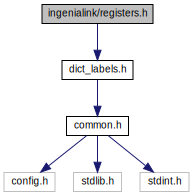
\includegraphics[width=265pt]{registers_8h__incl}
\end{center}
\end{figure}
This graph shows which files directly or indirectly include this file\+:\nopagebreak
\begin{figure}[H]
\begin{center}
\leavevmode
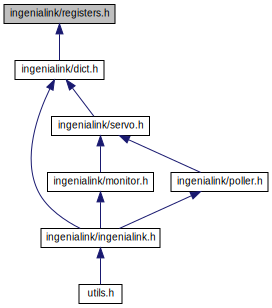
\includegraphics[width=344pt]{registers_8h__dep__incl}
\end{center}
\end{figure}
\subsection*{Data Structures}
\begin{DoxyCompactItemize}
\item 
union \hyperlink{unionil__reg__limit__t}{il\+\_\+reg\+\_\+limit\+\_\+t}
\begin{DoxyCompactList}\small\item\em Limits. \end{DoxyCompactList}\item 
struct \hyperlink{structil__reg__range__t}{il\+\_\+reg\+\_\+range\+\_\+t}
\begin{DoxyCompactList}\small\item\em Range. \end{DoxyCompactList}\item 
struct \hyperlink{structil__reg__t}{il\+\_\+reg\+\_\+t}
\begin{DoxyCompactList}\small\item\em Register. \end{DoxyCompactList}\end{DoxyCompactItemize}
\subsection*{Enumerations}
\begin{DoxyCompactItemize}
\item 
enum \hyperlink{group__IL__REGS_gaddd7edef254d348f2e8a48c40840cdd6}{il\+\_\+reg\+\_\+dtype\+\_\+t} \{ \\*
\hyperlink{group__IL__REGS_ggaddd7edef254d348f2e8a48c40840cdd6afebd31a475c6cb6b6c9ac200fd90a09b}{I\+L\+\_\+\+R\+E\+G\+\_\+\+D\+T\+Y\+P\+E\+\_\+\+U8}, 
\hyperlink{group__IL__REGS_ggaddd7edef254d348f2e8a48c40840cdd6a4d3f76f5e0e716d7b358d819691e834a}{I\+L\+\_\+\+R\+E\+G\+\_\+\+D\+T\+Y\+P\+E\+\_\+\+S8}, 
\hyperlink{group__IL__REGS_ggaddd7edef254d348f2e8a48c40840cdd6a4776d418653151a6cadd41574d631bfa}{I\+L\+\_\+\+R\+E\+G\+\_\+\+D\+T\+Y\+P\+E\+\_\+\+U16}, 
\hyperlink{group__IL__REGS_ggaddd7edef254d348f2e8a48c40840cdd6a3eb3b654856f84234168d58355e83a85}{I\+L\+\_\+\+R\+E\+G\+\_\+\+D\+T\+Y\+P\+E\+\_\+\+S16}, 
\\*
\hyperlink{group__IL__REGS_ggaddd7edef254d348f2e8a48c40840cdd6a3d299c6c4bbda29b3286a3483271ee90}{I\+L\+\_\+\+R\+E\+G\+\_\+\+D\+T\+Y\+P\+E\+\_\+\+U32}, 
\hyperlink{group__IL__REGS_ggaddd7edef254d348f2e8a48c40840cdd6aaf16d13caf933d3e002054de7a0f1c48}{I\+L\+\_\+\+R\+E\+G\+\_\+\+D\+T\+Y\+P\+E\+\_\+\+S32}, 
\hyperlink{group__IL__REGS_ggaddd7edef254d348f2e8a48c40840cdd6a5a0f02c573b8800ee8f113160ce93712}{I\+L\+\_\+\+R\+E\+G\+\_\+\+D\+T\+Y\+P\+E\+\_\+\+U64}, 
\hyperlink{group__IL__REGS_ggaddd7edef254d348f2e8a48c40840cdd6a37398082dc9828038d3403ca24a28d5a}{I\+L\+\_\+\+R\+E\+G\+\_\+\+D\+T\+Y\+P\+E\+\_\+\+S64}, 
\\*
\hyperlink{group__IL__REGS_ggaddd7edef254d348f2e8a48c40840cdd6a07e3bbcf6a1d00d8f62887e41b529239}{I\+L\+\_\+\+R\+E\+G\+\_\+\+D\+T\+Y\+P\+E\+\_\+\+F\+L\+O\+AT}, 
\hyperlink{group__IL__REGS_ggaddd7edef254d348f2e8a48c40840cdd6aeb15ea8dd9961e96edebfc3d0f36fbd3}{I\+L\+\_\+\+R\+E\+G\+\_\+\+D\+T\+Y\+P\+E\+\_\+\+S\+TR}
 \}\begin{DoxyCompactList}\small\item\em Register data type. \end{DoxyCompactList}
\item 
enum \hyperlink{group__IL__REGS_ga4c623bd7d0d5f059dd91949c6948147e}{il\+\_\+reg\+\_\+access\+\_\+t} \{ \hyperlink{group__IL__REGS_gga4c623bd7d0d5f059dd91949c6948147eafa388eb7ec6166ba6a59d0d665f3ac53}{I\+L\+\_\+\+R\+E\+G\+\_\+\+A\+C\+C\+E\+S\+S\+\_\+\+RW}, 
\hyperlink{group__IL__REGS_gga4c623bd7d0d5f059dd91949c6948147ea12dabd43c525dfea5fb20914711168b8}{I\+L\+\_\+\+R\+E\+G\+\_\+\+A\+C\+C\+E\+S\+S\+\_\+\+RO}, 
\hyperlink{group__IL__REGS_gga4c623bd7d0d5f059dd91949c6948147eadb0026436ae70de8a60920c1085561bb}{I\+L\+\_\+\+R\+E\+G\+\_\+\+A\+C\+C\+E\+S\+S\+\_\+\+WO}
 \}\begin{DoxyCompactList}\small\item\em Register access. \end{DoxyCompactList}
\item 
enum \hyperlink{group__IL__REGS_ga37538453e5c3d84733c628987a579590}{il\+\_\+reg\+\_\+phy\+\_\+t} \{ \\*
\hyperlink{group__IL__REGS_gga37538453e5c3d84733c628987a579590a34d96ac8a7b9afc02256a03d5a464822}{I\+L\+\_\+\+R\+E\+G\+\_\+\+P\+H\+Y\+\_\+\+N\+O\+NE}, 
\hyperlink{group__IL__REGS_gga37538453e5c3d84733c628987a579590a799176bbdcea555949cd68969361bc8f}{I\+L\+\_\+\+R\+E\+G\+\_\+\+P\+H\+Y\+\_\+\+T\+O\+R\+Q\+UE}, 
\hyperlink{group__IL__REGS_gga37538453e5c3d84733c628987a579590ad7bdcaae981dfbbd28c46bed55f947ac}{I\+L\+\_\+\+R\+E\+G\+\_\+\+P\+H\+Y\+\_\+\+P\+OS}, 
\hyperlink{group__IL__REGS_gga37538453e5c3d84733c628987a579590aea1c9cf80466e862af6a3a6f687550ef}{I\+L\+\_\+\+R\+E\+G\+\_\+\+P\+H\+Y\+\_\+\+V\+EL}, 
\\*
\hyperlink{group__IL__REGS_gga37538453e5c3d84733c628987a579590a3dc604058c640ad2997c5d4a1ad37b97}{I\+L\+\_\+\+R\+E\+G\+\_\+\+P\+H\+Y\+\_\+\+A\+CC}, 
\hyperlink{group__IL__REGS_gga37538453e5c3d84733c628987a579590a99385428e977da83262b2ad47bcfc8f0}{I\+L\+\_\+\+R\+E\+G\+\_\+\+P\+H\+Y\+\_\+\+V\+O\+L\+T\+\_\+\+R\+EL}, 
\hyperlink{group__IL__REGS_gga37538453e5c3d84733c628987a579590a0cad6fc9aa35ccf3b78d695f9a446e2e}{I\+L\+\_\+\+R\+E\+G\+\_\+\+P\+H\+Y\+\_\+\+R\+AD}
 \}\begin{DoxyCompactList}\small\item\em Register physical units type. \end{DoxyCompactList}
\end{DoxyCompactItemize}


\subsection{Detailed Description}
Registers. 


\hypertarget{servo_8h}{}\section{ingenialink/servo.h File Reference}
\label{servo_8h}\index{ingenialink/servo.\+h@{ingenialink/servo.\+h}}


Servo.  


{\ttfamily \#include \char`\"{}net.\+h\char`\"{}}\\*
{\ttfamily \#include \char`\"{}dict.\+h\char`\"{}}\\*
Include dependency graph for servo.\+h\+:\nopagebreak
\begin{figure}[H]
\begin{center}
\leavevmode
\includegraphics[width=280pt]{servo_8h__incl}
\end{center}
\end{figure}
This graph shows which files directly or indirectly include this file\+:\nopagebreak
\begin{figure}[H]
\begin{center}
\leavevmode
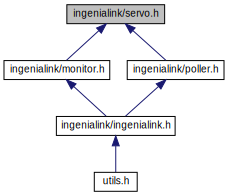
\includegraphics[width=301pt]{servo_8h__dep__incl}
\end{center}
\end{figure}
\subsection*{Data Structures}
\begin{DoxyCompactItemize}
\item 
struct \hyperlink{structil__servo__info__t}{il\+\_\+servo\+\_\+info\+\_\+t}
\begin{DoxyCompactList}\small\item\em Ingenia\+Link servo information. \end{DoxyCompactList}\end{DoxyCompactItemize}
\subsection*{Macros}
\begin{DoxyCompactItemize}
\item 
\#define \hyperlink{group__IL__SERVO_ga6c36d0853cb9bd4c71cee037421ec09a}{I\+L\+\_\+\+S\+E\+R\+V\+O\+\_\+\+S\+P\+\_\+\+T\+I\+M\+E\+O\+U\+T\+\_\+\+D\+EF}~1000
\begin{DoxyCompactList}\small\item\em Set-\/point acknowledge default timeout (ms). \end{DoxyCompactList}\item 
\#define \hyperlink{group__IL__SERVO_ga0a684ea427841d8ba4cf87b2d9a94d97}{I\+L\+\_\+\+S\+E\+R\+V\+O\+\_\+\+N\+A\+M\+E\+\_\+\+SZ}~9
\begin{DoxyCompactList}\small\item\em Servo name size (includes null termination). \end{DoxyCompactList}\item 
\#define \hyperlink{group__IL__SERVO_gaec19ad2892772d99664f16c55b9bc43f}{I\+L\+\_\+\+S\+E\+R\+V\+O\+\_\+\+S\+W\+\_\+\+V\+E\+R\+S\+I\+O\+N\+\_\+\+SZ}~9
\begin{DoxyCompactList}\small\item\em Servo software version size. \end{DoxyCompactList}\item 
\#define \hyperlink{group__IL__SERVO_ga18d9729ab800ffdda8ec81d8146a7e3f}{I\+L\+\_\+\+S\+E\+R\+V\+O\+\_\+\+H\+W\+\_\+\+V\+A\+R\+I\+A\+N\+T\+\_\+\+SZ}~5
\begin{DoxyCompactList}\small\item\em Hardware variant size. \end{DoxyCompactList}\item 
\#define \hyperlink{group__IL__SERVO_gaae195bbc7fd4c1d34122370e373a2fad}{I\+L\+\_\+\+S\+E\+R\+V\+O\+\_\+\+F\+L\+A\+G\+\_\+\+T\+G\+T\+\_\+\+R\+E\+A\+C\+H\+ED}~0x01
\begin{DoxyCompactList}\small\item\em Flags\+: Target reached. \end{DoxyCompactList}\item 
\#define \hyperlink{group__IL__SERVO_gac35b4c54f16936ff70f4e974a79fa586}{I\+L\+\_\+\+S\+E\+R\+V\+O\+\_\+\+F\+L\+A\+G\+\_\+\+I\+L\+I\+M\+\_\+\+A\+C\+T\+I\+VE}~0x02
\begin{DoxyCompactList}\small\item\em Flags\+: Internal limit active. \end{DoxyCompactList}\item 
\#define \hyperlink{group__IL__SERVO_ga683ef09e3c3e8133cfe1332a067cb88a}{I\+L\+\_\+\+S\+E\+R\+V\+O\+\_\+\+F\+L\+A\+G\+\_\+\+H\+O\+M\+I\+N\+G\+\_\+\+A\+TT}~0x04
\begin{DoxyCompactList}\small\item\em Flags\+: (Homing)\+: attained. \end{DoxyCompactList}\item 
\#define \hyperlink{group__IL__SERVO_gaa8b47a602774d828155efbc452bfbe66}{I\+L\+\_\+\+S\+E\+R\+V\+O\+\_\+\+F\+L\+A\+G\+\_\+\+H\+O\+M\+I\+N\+G\+\_\+\+E\+RR}~0x08
\begin{DoxyCompactList}\small\item\em Flags\+: (Homing)\+: error. \end{DoxyCompactList}\item 
\#define \hyperlink{group__IL__SERVO_gafa091abecc943d2133cd2a11bf1e6581}{I\+L\+\_\+\+S\+E\+R\+V\+O\+\_\+\+F\+L\+A\+G\+\_\+\+P\+V\+\_\+\+V\+Z\+E\+RO}~0x04
\begin{DoxyCompactList}\small\item\em Flags\+: (PV)\+: Vocity speed is zero. \end{DoxyCompactList}\item 
\#define \hyperlink{group__IL__SERVO_ga41e25c02b8b67f9d845f970cd6870144}{I\+L\+\_\+\+S\+E\+R\+V\+O\+\_\+\+F\+L\+A\+G\+\_\+\+P\+P\+\_\+\+S\+P\+A\+CK}~0x04
\begin{DoxyCompactList}\small\item\em Flags\+: (PP)\+: SP acknowledge. \end{DoxyCompactList}\item 
\#define \hyperlink{group__IL__SERVO_ga13208d747f34c53249e4e806dc1e88b9}{I\+L\+\_\+\+S\+E\+R\+V\+O\+\_\+\+F\+L\+A\+G\+\_\+\+I\+P\+\_\+\+A\+C\+T\+I\+VE}~0x04
\begin{DoxyCompactList}\small\item\em Flags\+: (IP)\+: active. \end{DoxyCompactList}\item 
\#define \hyperlink{group__IL__SERVO_gad862ccc1fcb5ee2969898185b2e8e10c}{I\+L\+\_\+\+S\+E\+R\+V\+O\+\_\+\+F\+L\+A\+G\+\_\+\+C\+S\+\_\+\+F\+O\+L\+L\+O\+WS}~0x04
\begin{DoxyCompactList}\small\item\em Flags\+: (C\+S\+T/\+C\+S\+V/\+C\+SP)\+: follow command value. \end{DoxyCompactList}\item 
\#define \hyperlink{group__IL__SERVO_gaa782f00113ceb5b0582471b8fe86a628}{I\+L\+\_\+\+S\+E\+R\+V\+O\+\_\+\+F\+L\+A\+G\+\_\+\+F\+E\+RR}~0x08
\begin{DoxyCompactList}\small\item\em Flags\+: (C\+S\+T/\+C\+S\+V/\+C\+S\+P/\+PV)\+: following error. \end{DoxyCompactList}\item 
\#define \hyperlink{group__IL__SERVO_gab8b5ab2cb8696d4781296b15ed4e0b67}{I\+L\+\_\+\+S\+E\+R\+V\+O\+\_\+\+F\+L\+A\+G\+\_\+\+I\+A\+N\+G\+L\+E\+\_\+\+D\+ET}~0x10
\begin{DoxyCompactList}\small\item\em Flags\+: Initial angle determination finished. \end{DoxyCompactList}\end{DoxyCompactItemize}
\subsection*{Typedefs}
\begin{DoxyCompactItemize}
\item 
typedef struct il\+\_\+servo \hyperlink{group__IL__SERVO_ga3369ddfcc33492fe3a28f96cf455b13e}{il\+\_\+servo\+\_\+t}
\begin{DoxyCompactList}\small\item\em Ingenia\+Link servo instance. \end{DoxyCompactList}\item 
typedef void($\ast$ \hyperlink{group__IL__SERVO_gad86cbd352b4ca4f73aa5bddece082a11}{il\+\_\+servo\+\_\+emcy\+\_\+subscriber\+\_\+cb\+\_\+t}) (void $\ast$ctx, uint32\+\_\+t code)
\begin{DoxyCompactList}\small\item\em Emergency subscriber callback. \end{DoxyCompactList}\item 
typedef void($\ast$ \hyperlink{group__IL__SERVO_ga60c0557ef5bc4c9e1b3bd32ea8d82861}{il\+\_\+servo\+\_\+state\+\_\+subscriber\+\_\+cb\+\_\+t}) (void $\ast$ctx, \hyperlink{group__IL__SERVO_ga34dfa4c089ba4ee833652ac6c40acd0d}{il\+\_\+servo\+\_\+state\+\_\+t} state, int flags)
\begin{DoxyCompactList}\small\item\em State updates subcriber callback. \end{DoxyCompactList}\end{DoxyCompactItemize}
\subsection*{Enumerations}
\begin{DoxyCompactItemize}
\item 
enum \hyperlink{group__IL__SERVO_ga34dfa4c089ba4ee833652ac6c40acd0d}{il\+\_\+servo\+\_\+state\+\_\+t} \{ \\*
\hyperlink{group__IL__SERVO_gga34dfa4c089ba4ee833652ac6c40acd0daa55953b65ace09c3bed52d4114840f1b}{I\+L\+\_\+\+S\+E\+R\+V\+O\+\_\+\+S\+T\+A\+T\+E\+\_\+\+N\+R\+DY}, 
\hyperlink{group__IL__SERVO_gga34dfa4c089ba4ee833652ac6c40acd0da23788d6ca281a3fbfed7562d75667adb}{I\+L\+\_\+\+S\+E\+R\+V\+O\+\_\+\+S\+T\+A\+T\+E\+\_\+\+D\+I\+S\+A\+B\+L\+ED}, 
\hyperlink{group__IL__SERVO_gga34dfa4c089ba4ee833652ac6c40acd0da526abc40393aee63a777f94b1a50f111}{I\+L\+\_\+\+S\+E\+R\+V\+O\+\_\+\+S\+T\+A\+T\+E\+\_\+\+R\+DY}, 
\hyperlink{group__IL__SERVO_gga34dfa4c089ba4ee833652ac6c40acd0da7cb1afaed87d34d110581a9e89509fdf}{I\+L\+\_\+\+S\+E\+R\+V\+O\+\_\+\+S\+T\+A\+T\+E\+\_\+\+ON}, 
\\*
\hyperlink{group__IL__SERVO_gga34dfa4c089ba4ee833652ac6c40acd0dab2f6b57025214e40be9fc2e1d69de2a5}{I\+L\+\_\+\+S\+E\+R\+V\+O\+\_\+\+S\+T\+A\+T\+E\+\_\+\+E\+N\+A\+B\+L\+ED}, 
\hyperlink{group__IL__SERVO_gga34dfa4c089ba4ee833652ac6c40acd0da3710762734b06272b18529e200585583}{I\+L\+\_\+\+S\+E\+R\+V\+O\+\_\+\+S\+T\+A\+T\+E\+\_\+\+Q\+S\+T\+OP}, 
\hyperlink{group__IL__SERVO_gga34dfa4c089ba4ee833652ac6c40acd0daf1d3fe0fefb6aecadacee5fb599375c0}{I\+L\+\_\+\+S\+E\+R\+V\+O\+\_\+\+S\+T\+A\+T\+E\+\_\+\+F\+A\+U\+L\+TR}, 
\hyperlink{group__IL__SERVO_gga34dfa4c089ba4ee833652ac6c40acd0da0e2beb3184098ba502e34354910f63f2}{I\+L\+\_\+\+S\+E\+R\+V\+O\+\_\+\+S\+T\+A\+T\+E\+\_\+\+F\+A\+U\+LT}
 \}\begin{DoxyCompactList}\small\item\em Servo states (equivalent to CiA 402 P\+DS states). \end{DoxyCompactList}
\item 
enum \hyperlink{group__IL__SERVO_ga6b3323798a8f235c225cc1d0cd27840a}{il\+\_\+servo\+\_\+mode\+\_\+t} \{ \\*
\hyperlink{group__IL__SERVO_gga6b3323798a8f235c225cc1d0cd27840aad8133deaaf79c917b29d388cf921a651}{I\+L\+\_\+\+S\+E\+R\+V\+O\+\_\+\+M\+O\+D\+E\+\_\+\+O\+LV}, 
\hyperlink{group__IL__SERVO_gga6b3323798a8f235c225cc1d0cd27840aaf49b82b9a802bb2b87cca3c777e8a72c}{I\+L\+\_\+\+S\+E\+R\+V\+O\+\_\+\+M\+O\+D\+E\+\_\+\+O\+LS}, 
\hyperlink{group__IL__SERVO_gga6b3323798a8f235c225cc1d0cd27840aa84502500bb9e2800c8c3bad60f30afd0}{I\+L\+\_\+\+S\+E\+R\+V\+O\+\_\+\+M\+O\+D\+E\+\_\+\+PP}, 
\hyperlink{group__IL__SERVO_gga6b3323798a8f235c225cc1d0cd27840aac670ce9cc12333e0d8b89e7e63db0f89}{I\+L\+\_\+\+S\+E\+R\+V\+O\+\_\+\+M\+O\+D\+E\+\_\+\+V\+EL}, 
\\*
\hyperlink{group__IL__SERVO_gga6b3323798a8f235c225cc1d0cd27840aa06f037b862ba17dfaac425ab706acf95}{I\+L\+\_\+\+S\+E\+R\+V\+O\+\_\+\+M\+O\+D\+E\+\_\+\+PV}, 
\hyperlink{group__IL__SERVO_gga6b3323798a8f235c225cc1d0cd27840aaf8243c2a154a13c399e9d5631593ce46}{I\+L\+\_\+\+S\+E\+R\+V\+O\+\_\+\+M\+O\+D\+E\+\_\+\+PT}, 
\hyperlink{group__IL__SERVO_gga6b3323798a8f235c225cc1d0cd27840aaf9aac6909e0810beac63271839113826}{I\+L\+\_\+\+S\+E\+R\+V\+O\+\_\+\+M\+O\+D\+E\+\_\+\+H\+O\+M\+I\+NG}, 
\hyperlink{group__IL__SERVO_gga6b3323798a8f235c225cc1d0cd27840aabc5de579ff40d7907da075bd60ef21fe}{I\+L\+\_\+\+S\+E\+R\+V\+O\+\_\+\+M\+O\+D\+E\+\_\+\+IP}, 
\\*
\hyperlink{group__IL__SERVO_gga6b3323798a8f235c225cc1d0cd27840aa4d36b5943ed7ab1d82483b310edae793}{I\+L\+\_\+\+S\+E\+R\+V\+O\+\_\+\+M\+O\+D\+E\+\_\+\+C\+SP}, 
\hyperlink{group__IL__SERVO_gga6b3323798a8f235c225cc1d0cd27840aa31597c98bdff233ab9dd1e1a9a238a3d}{I\+L\+\_\+\+S\+E\+R\+V\+O\+\_\+\+M\+O\+D\+E\+\_\+\+C\+SV}, 
\hyperlink{group__IL__SERVO_gga6b3323798a8f235c225cc1d0cd27840aadd4e3ef7edae53f0318cdebd41a00c9e}{I\+L\+\_\+\+S\+E\+R\+V\+O\+\_\+\+M\+O\+D\+E\+\_\+\+C\+ST}
 \}\begin{DoxyCompactList}\small\item\em Servo operation modes. \end{DoxyCompactList}
\item 
enum \hyperlink{group__IL__SERVO_ga4fb6d5223f5364f40c8f5c8018a00124}{il\+\_\+units\+\_\+torque\+\_\+t} \{ \hyperlink{group__IL__SERVO_gga4fb6d5223f5364f40c8f5c8018a00124a71f0c47645aba7c025c07a3793308518}{I\+L\+\_\+\+U\+N\+I\+T\+S\+\_\+\+T\+O\+R\+Q\+U\+E\+\_\+\+N\+A\+T\+I\+VE}, 
\hyperlink{group__IL__SERVO_gga4fb6d5223f5364f40c8f5c8018a00124a1caf6439156aabc869a67bea25f763fb}{I\+L\+\_\+\+U\+N\+I\+T\+S\+\_\+\+T\+O\+R\+Q\+U\+E\+\_\+\+M\+NM}, 
\hyperlink{group__IL__SERVO_gga4fb6d5223f5364f40c8f5c8018a00124a4a90e995ce79534d786c11dac9313a27}{I\+L\+\_\+\+U\+N\+I\+T\+S\+\_\+\+T\+O\+R\+Q\+U\+E\+\_\+\+NM}
 \}\begin{DoxyCompactList}\small\item\em Torque units. \end{DoxyCompactList}
\item 
enum \hyperlink{group__IL__SERVO_gaefeeab7931ae00097627941a79950799}{il\+\_\+units\+\_\+pos\+\_\+t} \{ \\*
\hyperlink{group__IL__SERVO_ggaefeeab7931ae00097627941a79950799afd38e43a05097d89890d0a35ae80a358}{I\+L\+\_\+\+U\+N\+I\+T\+S\+\_\+\+P\+O\+S\+\_\+\+N\+A\+T\+I\+VE}, 
\hyperlink{group__IL__SERVO_ggaefeeab7931ae00097627941a79950799a7dc0b4f7d0f9c2798c5ea5f1d04a4a8e}{I\+L\+\_\+\+U\+N\+I\+T\+S\+\_\+\+P\+O\+S\+\_\+\+R\+EV}, 
\hyperlink{group__IL__SERVO_ggaefeeab7931ae00097627941a79950799a44823ab17da1a86475c6dc3c9e85fa21}{I\+L\+\_\+\+U\+N\+I\+T\+S\+\_\+\+P\+O\+S\+\_\+\+R\+AD}, 
\hyperlink{group__IL__SERVO_ggaefeeab7931ae00097627941a79950799ad5a21928f5565c58ec6631ef735a73d4}{I\+L\+\_\+\+U\+N\+I\+T\+S\+\_\+\+P\+O\+S\+\_\+\+D\+EG}, 
\\*
\hyperlink{group__IL__SERVO_ggaefeeab7931ae00097627941a79950799a7b579b4273215a053d229a696e7a6b8a}{I\+L\+\_\+\+U\+N\+I\+T\+S\+\_\+\+P\+O\+S\+\_\+\+UM}, 
\hyperlink{group__IL__SERVO_ggaefeeab7931ae00097627941a79950799acf3bb2d9c0c753cf8f284322d653c5f2}{I\+L\+\_\+\+U\+N\+I\+T\+S\+\_\+\+P\+O\+S\+\_\+\+MM}, 
\hyperlink{group__IL__SERVO_ggaefeeab7931ae00097627941a79950799af95dfbcc88b47ade30d5211dc6dee09e}{I\+L\+\_\+\+U\+N\+I\+T\+S\+\_\+\+P\+O\+S\+\_\+M}
 \}\begin{DoxyCompactList}\small\item\em Position units. \end{DoxyCompactList}
\item 
enum \hyperlink{group__IL__SERVO_ga548eebb728eb841e157b57f2063203ee}{il\+\_\+units\+\_\+vel\+\_\+t} \{ \\*
\hyperlink{group__IL__SERVO_gga548eebb728eb841e157b57f2063203eea31f1d954a42ad41c75135c52483dc0fd}{I\+L\+\_\+\+U\+N\+I\+T\+S\+\_\+\+V\+E\+L\+\_\+\+N\+A\+T\+I\+VE}, 
\hyperlink{group__IL__SERVO_gga548eebb728eb841e157b57f2063203eea7ddfb276f1013c053617d2c5693af2a6}{I\+L\+\_\+\+U\+N\+I\+T\+S\+\_\+\+V\+E\+L\+\_\+\+R\+PS}, 
\hyperlink{group__IL__SERVO_gga548eebb728eb841e157b57f2063203eea945ffbca76bb3c0a21df0f242d24e18f}{I\+L\+\_\+\+U\+N\+I\+T\+S\+\_\+\+V\+E\+L\+\_\+\+R\+PM}, 
\hyperlink{group__IL__SERVO_gga548eebb728eb841e157b57f2063203eea7190dcc107d465da9e2ed577bc8d8ceb}{I\+L\+\_\+\+U\+N\+I\+T\+S\+\_\+\+V\+E\+L\+\_\+\+R\+A\+D\+\_\+S}, 
\\*
\hyperlink{group__IL__SERVO_gga548eebb728eb841e157b57f2063203eeaefca3b85d079add8af939073f1c4a2ba}{I\+L\+\_\+\+U\+N\+I\+T\+S\+\_\+\+V\+E\+L\+\_\+\+D\+E\+G\+\_\+S}, 
\hyperlink{group__IL__SERVO_gga548eebb728eb841e157b57f2063203eea792e330590bc7e221d6ee25bda627b7b}{I\+L\+\_\+\+U\+N\+I\+T\+S\+\_\+\+V\+E\+L\+\_\+\+U\+M\+\_\+S}, 
\hyperlink{group__IL__SERVO_gga548eebb728eb841e157b57f2063203eeacf5c8357769c71a6e6ff05e9cea1da35}{I\+L\+\_\+\+U\+N\+I\+T\+S\+\_\+\+V\+E\+L\+\_\+\+M\+M\+\_\+S}, 
\hyperlink{group__IL__SERVO_gga548eebb728eb841e157b57f2063203eea61616522994f03fef6dd301affee83ba}{I\+L\+\_\+\+U\+N\+I\+T\+S\+\_\+\+V\+E\+L\+\_\+\+M\+\_\+S}
 \}\begin{DoxyCompactList}\small\item\em Velocity units. \end{DoxyCompactList}
\item 
enum \hyperlink{group__IL__SERVO_ga07f4e0f292d1d7b5a6f1fc5c35fc151f}{il\+\_\+units\+\_\+acc\+\_\+t} \{ \\*
\hyperlink{group__IL__SERVO_gga07f4e0f292d1d7b5a6f1fc5c35fc151fa2dbb4edbf87bf40d1bec4e6b819570e5}{I\+L\+\_\+\+U\+N\+I\+T\+S\+\_\+\+A\+C\+C\+\_\+\+N\+A\+T\+I\+VE}, 
\hyperlink{group__IL__SERVO_gga07f4e0f292d1d7b5a6f1fc5c35fc151fa8fef1361fab6dab1481859efbb3b1c48}{I\+L\+\_\+\+U\+N\+I\+T\+S\+\_\+\+A\+C\+C\+\_\+\+R\+E\+V\+\_\+\+S2}, 
\hyperlink{group__IL__SERVO_gga07f4e0f292d1d7b5a6f1fc5c35fc151fadb4738643811868f758c9297c1199c70}{I\+L\+\_\+\+U\+N\+I\+T\+S\+\_\+\+A\+C\+C\+\_\+\+R\+A\+D\+\_\+\+S2}, 
\hyperlink{group__IL__SERVO_gga07f4e0f292d1d7b5a6f1fc5c35fc151fa9140fe3bc3c29c442a2af102f43abb77}{I\+L\+\_\+\+U\+N\+I\+T\+S\+\_\+\+A\+C\+C\+\_\+\+D\+E\+G\+\_\+\+S2}, 
\\*
\hyperlink{group__IL__SERVO_gga07f4e0f292d1d7b5a6f1fc5c35fc151fab6ee667f66aaae98136b1bae969467f7}{I\+L\+\_\+\+U\+N\+I\+T\+S\+\_\+\+A\+C\+C\+\_\+\+U\+M\+\_\+\+S2}, 
\hyperlink{group__IL__SERVO_gga07f4e0f292d1d7b5a6f1fc5c35fc151fa1cf13cf16f774312a603493c2e9961e4}{I\+L\+\_\+\+U\+N\+I\+T\+S\+\_\+\+A\+C\+C\+\_\+\+M\+M\+\_\+\+S2}, 
\hyperlink{group__IL__SERVO_gga07f4e0f292d1d7b5a6f1fc5c35fc151fa4de34cd9765e5671b419237519d33ec9}{I\+L\+\_\+\+U\+N\+I\+T\+S\+\_\+\+A\+C\+C\+\_\+\+M\+\_\+\+S2}
 \}\begin{DoxyCompactList}\small\item\em Acceleration units. \end{DoxyCompactList}
\end{DoxyCompactItemize}
\subsection*{Functions}
\begin{DoxyCompactItemize}
\item 
\hyperlink{common_8h_a6bb629d26c52bfe10519ba3176853f47}{I\+L\+\_\+\+E\+X\+P\+O\+RT} \hyperlink{group__IL__SERVO_ga3369ddfcc33492fe3a28f96cf455b13e}{il\+\_\+servo\+\_\+t} $\ast$ \hyperlink{group__IL__SERVO_gaa3728b10386d3b9f67258a95cb3c2913}{il\+\_\+servo\+\_\+create} (\hyperlink{group__IL__NET_ga0657204ab779a5b7a504aa0b895d1ae6}{il\+\_\+net\+\_\+t} $\ast$net, uint16\+\_\+t id, const char $\ast$dict)
\begin{DoxyCompactList}\small\item\em Create Ingenia\+Link servo instance. \end{DoxyCompactList}\item 
\hyperlink{common_8h_a6bb629d26c52bfe10519ba3176853f47}{I\+L\+\_\+\+E\+X\+P\+O\+RT} void \hyperlink{group__IL__SERVO_gade6d6e8ae2488af2a6ae6a6c484eaf32}{il\+\_\+servo\+\_\+destroy} (\hyperlink{group__IL__SERVO_ga3369ddfcc33492fe3a28f96cf455b13e}{il\+\_\+servo\+\_\+t} $\ast$servo)
\begin{DoxyCompactList}\small\item\em Destroy an Ingenia\+Link servo instance. \end{DoxyCompactList}\item 
\hyperlink{common_8h_a6bb629d26c52bfe10519ba3176853f47}{I\+L\+\_\+\+E\+X\+P\+O\+RT} int \hyperlink{group__IL__SERVO_ga1d0ef8479c2144e2abd9f18d7a875a34}{il\+\_\+servo\+\_\+reset} (\hyperlink{group__IL__SERVO_ga3369ddfcc33492fe3a28f96cf455b13e}{il\+\_\+servo\+\_\+t} $\ast$servo)
\begin{DoxyCompactList}\small\item\em Reset servo. \end{DoxyCompactList}\item 
\hyperlink{common_8h_a6bb629d26c52bfe10519ba3176853f47}{I\+L\+\_\+\+E\+X\+P\+O\+RT} void \hyperlink{group__IL__SERVO_ga52d4dfa8d34a7cce329d997c8ee8c38a}{il\+\_\+servo\+\_\+state\+\_\+get} (\hyperlink{group__IL__SERVO_ga3369ddfcc33492fe3a28f96cf455b13e}{il\+\_\+servo\+\_\+t} $\ast$servo, \hyperlink{group__IL__SERVO_ga34dfa4c089ba4ee833652ac6c40acd0d}{il\+\_\+servo\+\_\+state\+\_\+t} $\ast$state, int $\ast$flags)
\begin{DoxyCompactList}\small\item\em Obtain current servo P\+DS state. \end{DoxyCompactList}\item 
\hyperlink{common_8h_a6bb629d26c52bfe10519ba3176853f47}{I\+L\+\_\+\+E\+X\+P\+O\+RT} int \hyperlink{group__IL__SERVO_gab48c5b7f3f359ab4ad358525e9f69d88}{il\+\_\+servo\+\_\+state\+\_\+subscribe} (\hyperlink{group__IL__SERVO_ga3369ddfcc33492fe3a28f96cf455b13e}{il\+\_\+servo\+\_\+t} $\ast$servo, \hyperlink{group__IL__SERVO_ga60c0557ef5bc4c9e1b3bd32ea8d82861}{il\+\_\+servo\+\_\+state\+\_\+subscriber\+\_\+cb\+\_\+t} cb, void $\ast$ctx)
\begin{DoxyCompactList}\small\item\em Subscribe to state changes (and operation flags). \end{DoxyCompactList}\item 
\hyperlink{common_8h_a6bb629d26c52bfe10519ba3176853f47}{I\+L\+\_\+\+E\+X\+P\+O\+RT} void \hyperlink{group__IL__SERVO_gab9badbee2d7c812fd70f36e54b33f102}{il\+\_\+servo\+\_\+state\+\_\+unsubscribe} (\hyperlink{group__IL__SERVO_ga3369ddfcc33492fe3a28f96cf455b13e}{il\+\_\+servo\+\_\+t} $\ast$servo, int slot)
\begin{DoxyCompactList}\small\item\em Unsubscribe from state changes. \end{DoxyCompactList}\item 
\hyperlink{common_8h_a6bb629d26c52bfe10519ba3176853f47}{I\+L\+\_\+\+E\+X\+P\+O\+RT} int \hyperlink{group__IL__SERVO_gad64153fedf0e2c82b88b545de2a1e134}{il\+\_\+servo\+\_\+emcy\+\_\+subscribe} (\hyperlink{group__IL__SERVO_ga3369ddfcc33492fe3a28f96cf455b13e}{il\+\_\+servo\+\_\+t} $\ast$servo, \hyperlink{group__IL__SERVO_gad86cbd352b4ca4f73aa5bddece082a11}{il\+\_\+servo\+\_\+emcy\+\_\+subscriber\+\_\+cb\+\_\+t} cb, void $\ast$ctx)
\begin{DoxyCompactList}\small\item\em Subscribe to emergency messages. \end{DoxyCompactList}\item 
\hyperlink{common_8h_a6bb629d26c52bfe10519ba3176853f47}{I\+L\+\_\+\+E\+X\+P\+O\+RT} void \hyperlink{group__IL__SERVO_ga2bfe5b7de979ba3a7339292afa7c0a3b}{il\+\_\+servo\+\_\+emcy\+\_\+unsubscribe} (\hyperlink{group__IL__SERVO_ga3369ddfcc33492fe3a28f96cf455b13e}{il\+\_\+servo\+\_\+t} $\ast$servo, int slot)
\begin{DoxyCompactList}\small\item\em Unubscribe from emergency messages. \end{DoxyCompactList}\item 
\hyperlink{common_8h_a6bb629d26c52bfe10519ba3176853f47}{I\+L\+\_\+\+E\+X\+P\+O\+RT} \hyperlink{group__IL__DICT_gac2cb8ba7974d8506df3017879572fc84}{il\+\_\+dict\+\_\+t} $\ast$ \hyperlink{group__IL__SERVO_ga396350b82f3aeef0950533871c2d1214}{il\+\_\+servo\+\_\+dict\+\_\+get} (\hyperlink{group__IL__SERVO_ga3369ddfcc33492fe3a28f96cf455b13e}{il\+\_\+servo\+\_\+t} $\ast$servo)
\begin{DoxyCompactList}\small\item\em Obtain servo dictionary. \end{DoxyCompactList}\item 
\hyperlink{common_8h_a6bb629d26c52bfe10519ba3176853f47}{I\+L\+\_\+\+E\+X\+P\+O\+RT} int \hyperlink{group__IL__SERVO_ga5598b379a48c330d7c76ffb109088403}{il\+\_\+servo\+\_\+dict\+\_\+load} (\hyperlink{group__IL__SERVO_ga3369ddfcc33492fe3a28f96cf455b13e}{il\+\_\+servo\+\_\+t} $\ast$servo, const char $\ast$dict)
\begin{DoxyCompactList}\small\item\em Load a dictionary to the servo. \end{DoxyCompactList}\item 
\hyperlink{common_8h_a6bb629d26c52bfe10519ba3176853f47}{I\+L\+\_\+\+E\+X\+P\+O\+RT} int \hyperlink{group__IL__SERVO_ga4154f5f19c2826449c4e01021a9fa061}{il\+\_\+servo\+\_\+name\+\_\+get} (\hyperlink{group__IL__SERVO_ga3369ddfcc33492fe3a28f96cf455b13e}{il\+\_\+servo\+\_\+t} $\ast$servo, char $\ast$name, size\+\_\+t sz)
\begin{DoxyCompactList}\small\item\em Obtain servo name. \end{DoxyCompactList}\item 
\hyperlink{common_8h_a6bb629d26c52bfe10519ba3176853f47}{I\+L\+\_\+\+E\+X\+P\+O\+RT} int \hyperlink{group__IL__SERVO_gadd8ffb5ac5efa38c62e2d480f4c90475}{il\+\_\+servo\+\_\+name\+\_\+set} (\hyperlink{group__IL__SERVO_ga3369ddfcc33492fe3a28f96cf455b13e}{il\+\_\+servo\+\_\+t} $\ast$servo, const char $\ast$name)
\begin{DoxyCompactList}\small\item\em Set servo name. \end{DoxyCompactList}\item 
\hyperlink{common_8h_a6bb629d26c52bfe10519ba3176853f47}{I\+L\+\_\+\+E\+X\+P\+O\+RT} int \hyperlink{group__IL__SERVO_gac10a7958e9f2c4ef31ba2df3d7b51168}{il\+\_\+servo\+\_\+info\+\_\+get} (\hyperlink{group__IL__SERVO_ga3369ddfcc33492fe3a28f96cf455b13e}{il\+\_\+servo\+\_\+t} $\ast$servo, \hyperlink{structil__servo__info__t}{il\+\_\+servo\+\_\+info\+\_\+t} $\ast$info)
\begin{DoxyCompactList}\small\item\em Obtain servo information. \end{DoxyCompactList}\item 
\hyperlink{common_8h_a6bb629d26c52bfe10519ba3176853f47}{I\+L\+\_\+\+E\+X\+P\+O\+RT} int \hyperlink{group__IL__SERVO_gab2f6c3652bfea0818a2087434c5d4f6b}{il\+\_\+servo\+\_\+store\+\_\+all} (\hyperlink{group__IL__SERVO_ga3369ddfcc33492fe3a28f96cf455b13e}{il\+\_\+servo\+\_\+t} $\ast$servo)
\begin{DoxyCompactList}\small\item\em Store all servo current parameters to the N\+VM. \end{DoxyCompactList}\item 
\hyperlink{common_8h_a6bb629d26c52bfe10519ba3176853f47}{I\+L\+\_\+\+E\+X\+P\+O\+RT} int \hyperlink{group__IL__SERVO_ga665618a8278570eb3e1f35eecaa38048}{il\+\_\+servo\+\_\+store\+\_\+comm} (\hyperlink{group__IL__SERVO_ga3369ddfcc33492fe3a28f96cf455b13e}{il\+\_\+servo\+\_\+t} $\ast$servo)
\begin{DoxyCompactList}\small\item\em Store all servo current communications parameters to the N\+VM. \end{DoxyCompactList}\item 
\hyperlink{common_8h_a6bb629d26c52bfe10519ba3176853f47}{I\+L\+\_\+\+E\+X\+P\+O\+RT} int \hyperlink{group__IL__SERVO_gaaf4d6d6a1d9f90feaf7783a4a8bb5042}{il\+\_\+servo\+\_\+store\+\_\+app} (\hyperlink{group__IL__SERVO_ga3369ddfcc33492fe3a28f96cf455b13e}{il\+\_\+servo\+\_\+t} $\ast$servo)
\begin{DoxyCompactList}\small\item\em Store all servo current application parameters to the N\+VM. \end{DoxyCompactList}\item 
\hyperlink{common_8h_a6bb629d26c52bfe10519ba3176853f47}{I\+L\+\_\+\+E\+X\+P\+O\+RT} int \hyperlink{group__IL__SERVO_ga8bdb970bbe4c05d2b3f1d78268789bb3}{il\+\_\+servo\+\_\+units\+\_\+update} (\hyperlink{group__IL__SERVO_ga3369ddfcc33492fe3a28f96cf455b13e}{il\+\_\+servo\+\_\+t} $\ast$servo)
\begin{DoxyCompactList}\small\item\em Update units scaling factors. \end{DoxyCompactList}\item 
\hyperlink{common_8h_a6bb629d26c52bfe10519ba3176853f47}{I\+L\+\_\+\+E\+X\+P\+O\+RT} double \hyperlink{group__IL__SERVO_gacde3271e378552034d8c0966ead4f941}{il\+\_\+servo\+\_\+units\+\_\+factor} (\hyperlink{group__IL__SERVO_ga3369ddfcc33492fe3a28f96cf455b13e}{il\+\_\+servo\+\_\+t} $\ast$servo, const \hyperlink{structil__reg__t}{il\+\_\+reg\+\_\+t} $\ast$reg)
\begin{DoxyCompactList}\small\item\em Obtain the units scale factor associated with the given register. \end{DoxyCompactList}\item 
\hyperlink{common_8h_a6bb629d26c52bfe10519ba3176853f47}{I\+L\+\_\+\+E\+X\+P\+O\+RT} \hyperlink{group__IL__SERVO_ga4fb6d5223f5364f40c8f5c8018a00124}{il\+\_\+units\+\_\+torque\+\_\+t} \hyperlink{group__IL__SERVO_gaf227fedcfd9602135cefd6bf240202c6}{il\+\_\+servo\+\_\+units\+\_\+torque\+\_\+get} (\hyperlink{group__IL__SERVO_ga3369ddfcc33492fe3a28f96cf455b13e}{il\+\_\+servo\+\_\+t} $\ast$servo)
\begin{DoxyCompactList}\small\item\em Get the torque units. \end{DoxyCompactList}\item 
\hyperlink{common_8h_a6bb629d26c52bfe10519ba3176853f47}{I\+L\+\_\+\+E\+X\+P\+O\+RT} void \hyperlink{group__IL__SERVO_gab5d0b378b678e0fd6d1a571eb90ab66f}{il\+\_\+servo\+\_\+units\+\_\+torque\+\_\+set} (\hyperlink{group__IL__SERVO_ga3369ddfcc33492fe3a28f96cf455b13e}{il\+\_\+servo\+\_\+t} $\ast$servo, \hyperlink{group__IL__SERVO_ga4fb6d5223f5364f40c8f5c8018a00124}{il\+\_\+units\+\_\+torque\+\_\+t} units)
\begin{DoxyCompactList}\small\item\em Set the torque units. \end{DoxyCompactList}\item 
\hyperlink{common_8h_a6bb629d26c52bfe10519ba3176853f47}{I\+L\+\_\+\+E\+X\+P\+O\+RT} \hyperlink{group__IL__SERVO_gaefeeab7931ae00097627941a79950799}{il\+\_\+units\+\_\+pos\+\_\+t} \hyperlink{group__IL__SERVO_gad561c34b2b3d7646e8cc9cb360e2f87e}{il\+\_\+servo\+\_\+units\+\_\+pos\+\_\+get} (\hyperlink{group__IL__SERVO_ga3369ddfcc33492fe3a28f96cf455b13e}{il\+\_\+servo\+\_\+t} $\ast$servo)
\begin{DoxyCompactList}\small\item\em Get the position units. \end{DoxyCompactList}\item 
\hyperlink{common_8h_a6bb629d26c52bfe10519ba3176853f47}{I\+L\+\_\+\+E\+X\+P\+O\+RT} void \hyperlink{group__IL__SERVO_ga1a64e31ed42e99bff4a577fc8b2ad076}{il\+\_\+servo\+\_\+units\+\_\+pos\+\_\+set} (\hyperlink{group__IL__SERVO_ga3369ddfcc33492fe3a28f96cf455b13e}{il\+\_\+servo\+\_\+t} $\ast$servo, \hyperlink{group__IL__SERVO_gaefeeab7931ae00097627941a79950799}{il\+\_\+units\+\_\+pos\+\_\+t} units)
\begin{DoxyCompactList}\small\item\em Set the position units. \end{DoxyCompactList}\item 
\hyperlink{common_8h_a6bb629d26c52bfe10519ba3176853f47}{I\+L\+\_\+\+E\+X\+P\+O\+RT} \hyperlink{group__IL__SERVO_ga548eebb728eb841e157b57f2063203ee}{il\+\_\+units\+\_\+vel\+\_\+t} \hyperlink{group__IL__SERVO_gaeb7615b200f236722ef98bf1b8b594c2}{il\+\_\+servo\+\_\+units\+\_\+vel\+\_\+get} (\hyperlink{group__IL__SERVO_ga3369ddfcc33492fe3a28f96cf455b13e}{il\+\_\+servo\+\_\+t} $\ast$servo)
\begin{DoxyCompactList}\small\item\em Get the velocity units. \end{DoxyCompactList}\item 
\hyperlink{common_8h_a6bb629d26c52bfe10519ba3176853f47}{I\+L\+\_\+\+E\+X\+P\+O\+RT} void \hyperlink{group__IL__SERVO_gacd15dfc7141865bcb63912888aad71ba}{il\+\_\+servo\+\_\+units\+\_\+vel\+\_\+set} (\hyperlink{group__IL__SERVO_ga3369ddfcc33492fe3a28f96cf455b13e}{il\+\_\+servo\+\_\+t} $\ast$servo, \hyperlink{group__IL__SERVO_ga548eebb728eb841e157b57f2063203ee}{il\+\_\+units\+\_\+vel\+\_\+t} units)
\begin{DoxyCompactList}\small\item\em Set the velocity units. \end{DoxyCompactList}\item 
\hyperlink{common_8h_a6bb629d26c52bfe10519ba3176853f47}{I\+L\+\_\+\+E\+X\+P\+O\+RT} \hyperlink{group__IL__SERVO_ga07f4e0f292d1d7b5a6f1fc5c35fc151f}{il\+\_\+units\+\_\+acc\+\_\+t} \hyperlink{group__IL__SERVO_ga312b0ca5ea200c5ec1c60adad84017a2}{il\+\_\+servo\+\_\+units\+\_\+acc\+\_\+get} (\hyperlink{group__IL__SERVO_ga3369ddfcc33492fe3a28f96cf455b13e}{il\+\_\+servo\+\_\+t} $\ast$servo)
\begin{DoxyCompactList}\small\item\em Get the acceleration units. \end{DoxyCompactList}\item 
\hyperlink{common_8h_a6bb629d26c52bfe10519ba3176853f47}{I\+L\+\_\+\+E\+X\+P\+O\+RT} void \hyperlink{group__IL__SERVO_gae06520e0e95dc18d1586c6b76d303b80}{il\+\_\+servo\+\_\+units\+\_\+acc\+\_\+set} (\hyperlink{group__IL__SERVO_ga3369ddfcc33492fe3a28f96cf455b13e}{il\+\_\+servo\+\_\+t} $\ast$servo, \hyperlink{group__IL__SERVO_ga07f4e0f292d1d7b5a6f1fc5c35fc151f}{il\+\_\+units\+\_\+acc\+\_\+t} units)
\begin{DoxyCompactList}\small\item\em Set the acceleration units. \end{DoxyCompactList}\item 
\hyperlink{common_8h_a6bb629d26c52bfe10519ba3176853f47}{I\+L\+\_\+\+E\+X\+P\+O\+RT} int \hyperlink{group__IL__SERVO_ga8b1bd006fa9cd70b20097f723891122b}{il\+\_\+servo\+\_\+raw\+\_\+read\+\_\+u8} (\hyperlink{group__IL__SERVO_ga3369ddfcc33492fe3a28f96cf455b13e}{il\+\_\+servo\+\_\+t} $\ast$servo, const \hyperlink{structil__reg__t}{il\+\_\+reg\+\_\+t} $\ast$reg, const char $\ast$id, uint8\+\_\+t $\ast$buf)
\begin{DoxyCompactList}\small\item\em Read unsigned 8-\/bit value from a register. \end{DoxyCompactList}\item 
\hyperlink{common_8h_a6bb629d26c52bfe10519ba3176853f47}{I\+L\+\_\+\+E\+X\+P\+O\+RT} int \hyperlink{group__IL__SERVO_ga1d6b70bd773328b9cd7e63adcb5fdb24}{il\+\_\+servo\+\_\+raw\+\_\+read\+\_\+s8} (\hyperlink{group__IL__SERVO_ga3369ddfcc33492fe3a28f96cf455b13e}{il\+\_\+servo\+\_\+t} $\ast$servo, const \hyperlink{structil__reg__t}{il\+\_\+reg\+\_\+t} $\ast$reg, const char $\ast$id, int8\+\_\+t $\ast$buf)
\begin{DoxyCompactList}\small\item\em Read signed 8-\/bit value from a register. \end{DoxyCompactList}\item 
\hyperlink{common_8h_a6bb629d26c52bfe10519ba3176853f47}{I\+L\+\_\+\+E\+X\+P\+O\+RT} int \hyperlink{group__IL__SERVO_gae62ff2541783a740d8c2b623e489a703}{il\+\_\+servo\+\_\+raw\+\_\+read\+\_\+u16} (\hyperlink{group__IL__SERVO_ga3369ddfcc33492fe3a28f96cf455b13e}{il\+\_\+servo\+\_\+t} $\ast$servo, const \hyperlink{structil__reg__t}{il\+\_\+reg\+\_\+t} $\ast$reg, const char $\ast$id, uint16\+\_\+t $\ast$buf)
\begin{DoxyCompactList}\small\item\em Read unsigned 16-\/bit value from a register. \end{DoxyCompactList}\item 
\hyperlink{common_8h_a6bb629d26c52bfe10519ba3176853f47}{I\+L\+\_\+\+E\+X\+P\+O\+RT} int \hyperlink{group__IL__SERVO_ga9ac45aa67ec61b0dcbe2827a4484bfd5}{il\+\_\+servo\+\_\+raw\+\_\+read\+\_\+s16} (\hyperlink{group__IL__SERVO_ga3369ddfcc33492fe3a28f96cf455b13e}{il\+\_\+servo\+\_\+t} $\ast$servo, const \hyperlink{structil__reg__t}{il\+\_\+reg\+\_\+t} $\ast$reg, const char $\ast$id, int16\+\_\+t $\ast$buf)
\begin{DoxyCompactList}\small\item\em Read signed 16-\/bit value from a register. \end{DoxyCompactList}\item 
\hyperlink{common_8h_a6bb629d26c52bfe10519ba3176853f47}{I\+L\+\_\+\+E\+X\+P\+O\+RT} int \hyperlink{group__IL__SERVO_ga887a2e63754e1a4ebee5a0ab8310cc56}{il\+\_\+servo\+\_\+raw\+\_\+read\+\_\+u32} (\hyperlink{group__IL__SERVO_ga3369ddfcc33492fe3a28f96cf455b13e}{il\+\_\+servo\+\_\+t} $\ast$servo, const \hyperlink{structil__reg__t}{il\+\_\+reg\+\_\+t} $\ast$reg, const char $\ast$id, uint32\+\_\+t $\ast$buf)
\begin{DoxyCompactList}\small\item\em Read unsigned 32-\/bit value from a register. \end{DoxyCompactList}\item 
\hyperlink{common_8h_a6bb629d26c52bfe10519ba3176853f47}{I\+L\+\_\+\+E\+X\+P\+O\+RT} int \hyperlink{group__IL__SERVO_gab0c5bbb4fcd2784f10fab3648dc405c4}{il\+\_\+servo\+\_\+raw\+\_\+read\+\_\+s32} (\hyperlink{group__IL__SERVO_ga3369ddfcc33492fe3a28f96cf455b13e}{il\+\_\+servo\+\_\+t} $\ast$servo, const \hyperlink{structil__reg__t}{il\+\_\+reg\+\_\+t} $\ast$reg, const char $\ast$id, int32\+\_\+t $\ast$buf)
\begin{DoxyCompactList}\small\item\em Read signed 32-\/bit value from a register. \end{DoxyCompactList}\item 
\hyperlink{common_8h_a6bb629d26c52bfe10519ba3176853f47}{I\+L\+\_\+\+E\+X\+P\+O\+RT} int \hyperlink{group__IL__SERVO_ga254f9ed1043d3cc6e7175b0bb6a0c2c9}{il\+\_\+servo\+\_\+raw\+\_\+read\+\_\+u64} (\hyperlink{group__IL__SERVO_ga3369ddfcc33492fe3a28f96cf455b13e}{il\+\_\+servo\+\_\+t} $\ast$servo, const \hyperlink{structil__reg__t}{il\+\_\+reg\+\_\+t} $\ast$reg, const char $\ast$id, uint64\+\_\+t $\ast$buf)
\begin{DoxyCompactList}\small\item\em Read unsigned 64-\/bit value from a register. \end{DoxyCompactList}\item 
\hyperlink{common_8h_a6bb629d26c52bfe10519ba3176853f47}{I\+L\+\_\+\+E\+X\+P\+O\+RT} int \hyperlink{group__IL__SERVO_ga5caadeb6cb861b7a8b91dbb98113988f}{il\+\_\+servo\+\_\+raw\+\_\+read\+\_\+s64} (\hyperlink{group__IL__SERVO_ga3369ddfcc33492fe3a28f96cf455b13e}{il\+\_\+servo\+\_\+t} $\ast$servo, const \hyperlink{structil__reg__t}{il\+\_\+reg\+\_\+t} $\ast$reg, const char $\ast$id, int64\+\_\+t $\ast$buf)
\begin{DoxyCompactList}\small\item\em Read signed 64-\/bit value from a register. \end{DoxyCompactList}\item 
\hyperlink{common_8h_a6bb629d26c52bfe10519ba3176853f47}{I\+L\+\_\+\+E\+X\+P\+O\+RT} int \hyperlink{group__IL__SERVO_gacf0d6571be514e23c09581834203d90e}{il\+\_\+servo\+\_\+raw\+\_\+read\+\_\+float} (\hyperlink{group__IL__SERVO_ga3369ddfcc33492fe3a28f96cf455b13e}{il\+\_\+servo\+\_\+t} $\ast$servo, const \hyperlink{structil__reg__t}{il\+\_\+reg\+\_\+t} $\ast$reg, const char $\ast$id, float $\ast$buf)
\begin{DoxyCompactList}\small\item\em Read signed 64-\/bit value from a register. \end{DoxyCompactList}\item 
\hyperlink{common_8h_a6bb629d26c52bfe10519ba3176853f47}{I\+L\+\_\+\+E\+X\+P\+O\+RT} int \hyperlink{group__IL__SERVO_gad3b94f5a9811dd5a52bb306e92f92944}{il\+\_\+servo\+\_\+read} (\hyperlink{group__IL__SERVO_ga3369ddfcc33492fe3a28f96cf455b13e}{il\+\_\+servo\+\_\+t} $\ast$servo, const \hyperlink{structil__reg__t}{il\+\_\+reg\+\_\+t} $\ast$reg, const char $\ast$id, double $\ast$buf)
\begin{DoxyCompactList}\small\item\em Read a register. \end{DoxyCompactList}\item 
\hyperlink{common_8h_a6bb629d26c52bfe10519ba3176853f47}{I\+L\+\_\+\+E\+X\+P\+O\+RT} int \hyperlink{group__IL__SERVO_ga05c1c7c4d30c882744008de007686f3f}{il\+\_\+servo\+\_\+raw\+\_\+write\+\_\+u8} (\hyperlink{group__IL__SERVO_ga3369ddfcc33492fe3a28f96cf455b13e}{il\+\_\+servo\+\_\+t} $\ast$servo, const \hyperlink{structil__reg__t}{il\+\_\+reg\+\_\+t} $\ast$reg, const char $\ast$id, uint8\+\_\+t val, int confirm)
\begin{DoxyCompactList}\small\item\em Write unsigned 8-\/bit integer to a register. \end{DoxyCompactList}\item 
\hyperlink{common_8h_a6bb629d26c52bfe10519ba3176853f47}{I\+L\+\_\+\+E\+X\+P\+O\+RT} int \hyperlink{group__IL__SERVO_gafea21fc3b0adb4208a0571c87f979c50}{il\+\_\+servo\+\_\+raw\+\_\+write\+\_\+s8} (\hyperlink{group__IL__SERVO_ga3369ddfcc33492fe3a28f96cf455b13e}{il\+\_\+servo\+\_\+t} $\ast$servo, const \hyperlink{structil__reg__t}{il\+\_\+reg\+\_\+t} $\ast$reg, const char $\ast$id, int8\+\_\+t val, int confirm)
\begin{DoxyCompactList}\small\item\em Write signed 8-\/bit integer to a register. \end{DoxyCompactList}\item 
\hyperlink{common_8h_a6bb629d26c52bfe10519ba3176853f47}{I\+L\+\_\+\+E\+X\+P\+O\+RT} int \hyperlink{group__IL__SERVO_gae504512849138dc97ab7e5c51a1a6a02}{il\+\_\+servo\+\_\+raw\+\_\+write\+\_\+u16} (\hyperlink{group__IL__SERVO_ga3369ddfcc33492fe3a28f96cf455b13e}{il\+\_\+servo\+\_\+t} $\ast$servo, const \hyperlink{structil__reg__t}{il\+\_\+reg\+\_\+t} $\ast$reg, const char $\ast$id, uint16\+\_\+t val, int confirm)
\begin{DoxyCompactList}\small\item\em Write unsigned 16-\/bit integer to a register. \end{DoxyCompactList}\item 
\hyperlink{common_8h_a6bb629d26c52bfe10519ba3176853f47}{I\+L\+\_\+\+E\+X\+P\+O\+RT} int \hyperlink{group__IL__SERVO_ga42b17982936b1ce7982e5d16c3f6c090}{il\+\_\+servo\+\_\+raw\+\_\+write\+\_\+s16} (\hyperlink{group__IL__SERVO_ga3369ddfcc33492fe3a28f96cf455b13e}{il\+\_\+servo\+\_\+t} $\ast$servo, const \hyperlink{structil__reg__t}{il\+\_\+reg\+\_\+t} $\ast$reg, const char $\ast$id, int16\+\_\+t val, int confirm)
\begin{DoxyCompactList}\small\item\em Write signed 16-\/bit integer to a register. \end{DoxyCompactList}\item 
\hyperlink{common_8h_a6bb629d26c52bfe10519ba3176853f47}{I\+L\+\_\+\+E\+X\+P\+O\+RT} int \hyperlink{group__IL__SERVO_gac212376609f84669eb9792b676f453a3}{il\+\_\+servo\+\_\+raw\+\_\+write\+\_\+u32} (\hyperlink{group__IL__SERVO_ga3369ddfcc33492fe3a28f96cf455b13e}{il\+\_\+servo\+\_\+t} $\ast$servo, const \hyperlink{structil__reg__t}{il\+\_\+reg\+\_\+t} $\ast$reg, const char $\ast$id, uint32\+\_\+t val, int confirm)
\begin{DoxyCompactList}\small\item\em Write unsigned 32-\/bit integer to a register. \end{DoxyCompactList}\item 
\hyperlink{common_8h_a6bb629d26c52bfe10519ba3176853f47}{I\+L\+\_\+\+E\+X\+P\+O\+RT} int \hyperlink{group__IL__SERVO_gac07e7c8a81f9905d1fa9b447395270bc}{il\+\_\+servo\+\_\+raw\+\_\+write\+\_\+s32} (\hyperlink{group__IL__SERVO_ga3369ddfcc33492fe3a28f96cf455b13e}{il\+\_\+servo\+\_\+t} $\ast$servo, const \hyperlink{structil__reg__t}{il\+\_\+reg\+\_\+t} $\ast$reg, const char $\ast$id, int32\+\_\+t val, int confirm)
\begin{DoxyCompactList}\small\item\em Write signed 32-\/bit integer to a register. \end{DoxyCompactList}\item 
\hyperlink{common_8h_a6bb629d26c52bfe10519ba3176853f47}{I\+L\+\_\+\+E\+X\+P\+O\+RT} int \hyperlink{group__IL__SERVO_gacd041c7dd2ac1ec99d2cf1aa6f046a00}{il\+\_\+servo\+\_\+raw\+\_\+write\+\_\+u64} (\hyperlink{group__IL__SERVO_ga3369ddfcc33492fe3a28f96cf455b13e}{il\+\_\+servo\+\_\+t} $\ast$servo, const \hyperlink{structil__reg__t}{il\+\_\+reg\+\_\+t} $\ast$reg, const char $\ast$id, uint64\+\_\+t val, int confirm)
\begin{DoxyCompactList}\small\item\em Write unsigned 64-\/bit integer to a register. \end{DoxyCompactList}\item 
\hyperlink{common_8h_a6bb629d26c52bfe10519ba3176853f47}{I\+L\+\_\+\+E\+X\+P\+O\+RT} int \hyperlink{group__IL__SERVO_ga4ac4489c10367847a0d62d53ebf25a60}{il\+\_\+servo\+\_\+raw\+\_\+write\+\_\+s64} (\hyperlink{group__IL__SERVO_ga3369ddfcc33492fe3a28f96cf455b13e}{il\+\_\+servo\+\_\+t} $\ast$servo, const \hyperlink{structil__reg__t}{il\+\_\+reg\+\_\+t} $\ast$reg, const char $\ast$id, int64\+\_\+t val, int confirm)
\begin{DoxyCompactList}\small\item\em Write signed 64-\/bit integer to a register. \end{DoxyCompactList}\item 
\hyperlink{common_8h_a6bb629d26c52bfe10519ba3176853f47}{I\+L\+\_\+\+E\+X\+P\+O\+RT} int \hyperlink{group__IL__SERVO_ga56da0b13de04887cc5a6f9b2d4e7497e}{il\+\_\+servo\+\_\+raw\+\_\+write\+\_\+float} (\hyperlink{group__IL__SERVO_ga3369ddfcc33492fe3a28f96cf455b13e}{il\+\_\+servo\+\_\+t} $\ast$servo, const \hyperlink{structil__reg__t}{il\+\_\+reg\+\_\+t} $\ast$reg, const char $\ast$id, float val, int confirm)
\begin{DoxyCompactList}\small\item\em Write float to a register. \end{DoxyCompactList}\item 
\hyperlink{common_8h_a6bb629d26c52bfe10519ba3176853f47}{I\+L\+\_\+\+E\+X\+P\+O\+RT} int \hyperlink{group__IL__SERVO_gad1474e21342f4f02e6435d3f6d66dec1}{il\+\_\+servo\+\_\+write} (\hyperlink{group__IL__SERVO_ga3369ddfcc33492fe3a28f96cf455b13e}{il\+\_\+servo\+\_\+t} $\ast$servo, const \hyperlink{structil__reg__t}{il\+\_\+reg\+\_\+t} $\ast$reg, const char $\ast$id, double val, int confirm)
\begin{DoxyCompactList}\small\item\em Write to a register. \end{DoxyCompactList}\item 
\hyperlink{common_8h_a6bb629d26c52bfe10519ba3176853f47}{I\+L\+\_\+\+E\+X\+P\+O\+RT} int \hyperlink{group__IL__SERVO_ga8b5938454ac8183a514d11203f2e6197}{il\+\_\+servo\+\_\+disable} (\hyperlink{group__IL__SERVO_ga3369ddfcc33492fe3a28f96cf455b13e}{il\+\_\+servo\+\_\+t} $\ast$servo)
\begin{DoxyCompactList}\small\item\em Disable servo P\+DS. \end{DoxyCompactList}\item 
\hyperlink{common_8h_a6bb629d26c52bfe10519ba3176853f47}{I\+L\+\_\+\+E\+X\+P\+O\+RT} int \hyperlink{group__IL__SERVO_ga9ad6a595ca932caf31c2500de1e8a812}{il\+\_\+servo\+\_\+switch\+\_\+on} (\hyperlink{group__IL__SERVO_ga3369ddfcc33492fe3a28f96cf455b13e}{il\+\_\+servo\+\_\+t} $\ast$servo, int timeout)
\begin{DoxyCompactList}\small\item\em Switch on servo P\+DS. \end{DoxyCompactList}\item 
\hyperlink{common_8h_a6bb629d26c52bfe10519ba3176853f47}{I\+L\+\_\+\+E\+X\+P\+O\+RT} int \hyperlink{group__IL__SERVO_gaee57b72c5f6d4756a6a914edbf0db0d9}{il\+\_\+servo\+\_\+enable} (\hyperlink{group__IL__SERVO_ga3369ddfcc33492fe3a28f96cf455b13e}{il\+\_\+servo\+\_\+t} $\ast$servo, int timeout)
\begin{DoxyCompactList}\small\item\em Enable servo P\+DS. \end{DoxyCompactList}\item 
\hyperlink{common_8h_a6bb629d26c52bfe10519ba3176853f47}{I\+L\+\_\+\+E\+X\+P\+O\+RT} int \hyperlink{group__IL__SERVO_ga75fbdd6046af1825619d2710580911e2}{il\+\_\+servo\+\_\+fault\+\_\+reset} (\hyperlink{group__IL__SERVO_ga3369ddfcc33492fe3a28f96cf455b13e}{il\+\_\+servo\+\_\+t} $\ast$servo)
\begin{DoxyCompactList}\small\item\em Reset the drive fault state. \end{DoxyCompactList}\item 
\hyperlink{common_8h_a6bb629d26c52bfe10519ba3176853f47}{I\+L\+\_\+\+E\+X\+P\+O\+RT} int \hyperlink{group__IL__SERVO_ga7f545d6dd93e52f55688bb03ee263004}{il\+\_\+servo\+\_\+mode\+\_\+get} (\hyperlink{group__IL__SERVO_ga3369ddfcc33492fe3a28f96cf455b13e}{il\+\_\+servo\+\_\+t} $\ast$servo, \hyperlink{group__IL__SERVO_ga6b3323798a8f235c225cc1d0cd27840a}{il\+\_\+servo\+\_\+mode\+\_\+t} $\ast$mode)
\begin{DoxyCompactList}\small\item\em Get the servo operation mode. \end{DoxyCompactList}\item 
\hyperlink{common_8h_a6bb629d26c52bfe10519ba3176853f47}{I\+L\+\_\+\+E\+X\+P\+O\+RT} int \hyperlink{group__IL__SERVO_ga9ef9a84e8b6aa1ee23d301dbd93b8b2f}{il\+\_\+servo\+\_\+mode\+\_\+set} (\hyperlink{group__IL__SERVO_ga3369ddfcc33492fe3a28f96cf455b13e}{il\+\_\+servo\+\_\+t} $\ast$servo, \hyperlink{group__IL__SERVO_ga6b3323798a8f235c225cc1d0cd27840a}{il\+\_\+servo\+\_\+mode\+\_\+t} mode)
\begin{DoxyCompactList}\small\item\em Set the servo operation mode. \end{DoxyCompactList}\item 
\hyperlink{common_8h_a6bb629d26c52bfe10519ba3176853f47}{I\+L\+\_\+\+E\+X\+P\+O\+RT} int \hyperlink{group__IL__SERVO_ga245d1c9ecdbee76adff2b79757ebf158}{il\+\_\+servo\+\_\+ol\+\_\+voltage\+\_\+get} (\hyperlink{group__IL__SERVO_ga3369ddfcc33492fe3a28f96cf455b13e}{il\+\_\+servo\+\_\+t} $\ast$servo, double $\ast$voltage)
\begin{DoxyCompactList}\small\item\em Get the open loop voltage. \end{DoxyCompactList}\item 
\hyperlink{common_8h_a6bb629d26c52bfe10519ba3176853f47}{I\+L\+\_\+\+E\+X\+P\+O\+RT} int \hyperlink{group__IL__SERVO_ga3aec778ff294237e8e32a651ec8e215d}{il\+\_\+servo\+\_\+ol\+\_\+voltage\+\_\+set} (\hyperlink{group__IL__SERVO_ga3369ddfcc33492fe3a28f96cf455b13e}{il\+\_\+servo\+\_\+t} $\ast$servo, double voltage)
\begin{DoxyCompactList}\small\item\em Set the open loop voltage. \end{DoxyCompactList}\item 
\hyperlink{common_8h_a6bb629d26c52bfe10519ba3176853f47}{I\+L\+\_\+\+E\+X\+P\+O\+RT} int \hyperlink{group__IL__SERVO_ga190f42e03d0a1255efd92df375690f02}{il\+\_\+servo\+\_\+ol\+\_\+frequency\+\_\+get} (\hyperlink{group__IL__SERVO_ga3369ddfcc33492fe3a28f96cf455b13e}{il\+\_\+servo\+\_\+t} $\ast$servo, double $\ast$freq)
\begin{DoxyCompactList}\small\item\em Get the open loop frequency. \end{DoxyCompactList}\item 
\hyperlink{common_8h_a6bb629d26c52bfe10519ba3176853f47}{I\+L\+\_\+\+E\+X\+P\+O\+RT} int \hyperlink{group__IL__SERVO_ga7032da0b86cc1f6b139f10993c567b8a}{il\+\_\+servo\+\_\+ol\+\_\+frequency\+\_\+set} (\hyperlink{group__IL__SERVO_ga3369ddfcc33492fe3a28f96cf455b13e}{il\+\_\+servo\+\_\+t} $\ast$servo, double freq)
\begin{DoxyCompactList}\small\item\em Set the open loop frequency. \end{DoxyCompactList}\item 
\hyperlink{common_8h_a6bb629d26c52bfe10519ba3176853f47}{I\+L\+\_\+\+E\+X\+P\+O\+RT} int \hyperlink{group__IL__SERVO_gaf7cf26ed91ae60e5f049b056009783e0}{il\+\_\+servo\+\_\+homing\+\_\+start} (\hyperlink{group__IL__SERVO_ga3369ddfcc33492fe3a28f96cf455b13e}{il\+\_\+servo\+\_\+t} $\ast$servo)
\begin{DoxyCompactList}\small\item\em Start homing. \end{DoxyCompactList}\item 
\hyperlink{common_8h_a6bb629d26c52bfe10519ba3176853f47}{I\+L\+\_\+\+E\+X\+P\+O\+RT} int \hyperlink{group__IL__SERVO_gad55d208e57e674e0c1a31b995563e96d}{il\+\_\+servo\+\_\+homing\+\_\+wait} (\hyperlink{group__IL__SERVO_ga3369ddfcc33492fe3a28f96cf455b13e}{il\+\_\+servo\+\_\+t} $\ast$servo, int timeout)
\begin{DoxyCompactList}\small\item\em Wait until homing completes. \end{DoxyCompactList}\item 
\hyperlink{common_8h_a6bb629d26c52bfe10519ba3176853f47}{I\+L\+\_\+\+E\+X\+P\+O\+RT} int \hyperlink{group__IL__SERVO_ga77eb2ebb33ac5bc9e3eac7b3ae90e25b}{il\+\_\+servo\+\_\+torque\+\_\+get} (\hyperlink{group__IL__SERVO_ga3369ddfcc33492fe3a28f96cf455b13e}{il\+\_\+servo\+\_\+t} $\ast$servo, double $\ast$torque)
\begin{DoxyCompactList}\small\item\em Get the actual servo torque. \end{DoxyCompactList}\item 
\hyperlink{common_8h_a6bb629d26c52bfe10519ba3176853f47}{I\+L\+\_\+\+E\+X\+P\+O\+RT} int \hyperlink{group__IL__SERVO_gaf5be5c151da47f8a017ee8fe667ad84f}{il\+\_\+servo\+\_\+torque\+\_\+set} (\hyperlink{group__IL__SERVO_ga3369ddfcc33492fe3a28f96cf455b13e}{il\+\_\+servo\+\_\+t} $\ast$servo, double torque)
\begin{DoxyCompactList}\small\item\em Set the servo target torque. \end{DoxyCompactList}\item 
\hyperlink{common_8h_a6bb629d26c52bfe10519ba3176853f47}{I\+L\+\_\+\+E\+X\+P\+O\+RT} int \hyperlink{group__IL__SERVO_gabf1b0cdad34399c230963e1e9783f419}{il\+\_\+servo\+\_\+position\+\_\+get} (\hyperlink{group__IL__SERVO_ga3369ddfcc33492fe3a28f96cf455b13e}{il\+\_\+servo\+\_\+t} $\ast$servo, double $\ast$pos)
\begin{DoxyCompactList}\small\item\em Get the actual servo position. \end{DoxyCompactList}\item 
\hyperlink{common_8h_a6bb629d26c52bfe10519ba3176853f47}{I\+L\+\_\+\+E\+X\+P\+O\+RT} int \hyperlink{group__IL__SERVO_ga24af5dbdebb7a56f73070781d53e2d76}{il\+\_\+servo\+\_\+position\+\_\+set} (\hyperlink{group__IL__SERVO_ga3369ddfcc33492fe3a28f96cf455b13e}{il\+\_\+servo\+\_\+t} $\ast$servo, double pos, int immediate, int relative, int sp\+\_\+timeout)
\begin{DoxyCompactList}\small\item\em Set the servo target position. \end{DoxyCompactList}\item 
\hyperlink{common_8h_a6bb629d26c52bfe10519ba3176853f47}{I\+L\+\_\+\+E\+X\+P\+O\+RT} int \hyperlink{group__IL__SERVO_ga34382a1fd3a11ae5f64e20399ee85356}{il\+\_\+servo\+\_\+position\+\_\+res\+\_\+get} (\hyperlink{group__IL__SERVO_ga3369ddfcc33492fe3a28f96cf455b13e}{il\+\_\+servo\+\_\+t} $\ast$servo, uint32\+\_\+t $\ast$res)
\begin{DoxyCompactList}\small\item\em Obtain position resolution. \end{DoxyCompactList}\item 
\hyperlink{common_8h_a6bb629d26c52bfe10519ba3176853f47}{I\+L\+\_\+\+E\+X\+P\+O\+RT} int \hyperlink{group__IL__SERVO_ga466d1762b8c9d773ce2b3697a44b3d0a}{il\+\_\+servo\+\_\+velocity\+\_\+get} (\hyperlink{group__IL__SERVO_ga3369ddfcc33492fe3a28f96cf455b13e}{il\+\_\+servo\+\_\+t} $\ast$servo, double $\ast$vel)
\begin{DoxyCompactList}\small\item\em Get the actual servo velocity. \end{DoxyCompactList}\item 
\hyperlink{common_8h_a6bb629d26c52bfe10519ba3176853f47}{I\+L\+\_\+\+E\+X\+P\+O\+RT} int \hyperlink{group__IL__SERVO_ga8831402af125c7706353d0dc9bf1364c}{il\+\_\+servo\+\_\+velocity\+\_\+set} (\hyperlink{group__IL__SERVO_ga3369ddfcc33492fe3a28f96cf455b13e}{il\+\_\+servo\+\_\+t} $\ast$servo, double vel)
\begin{DoxyCompactList}\small\item\em Set the servo target velocity. \end{DoxyCompactList}\item 
\hyperlink{common_8h_a6bb629d26c52bfe10519ba3176853f47}{I\+L\+\_\+\+E\+X\+P\+O\+RT} int \hyperlink{group__IL__SERVO_gac23b38d71bf5e26a1d5c275f9e711c47}{il\+\_\+servo\+\_\+velocity\+\_\+res\+\_\+get} (\hyperlink{group__IL__SERVO_ga3369ddfcc33492fe3a28f96cf455b13e}{il\+\_\+servo\+\_\+t} $\ast$servo, uint32\+\_\+t $\ast$res)
\begin{DoxyCompactList}\small\item\em Obtain velocity resolution. \end{DoxyCompactList}\item 
\hyperlink{common_8h_a6bb629d26c52bfe10519ba3176853f47}{I\+L\+\_\+\+E\+X\+P\+O\+RT} int \hyperlink{group__IL__SERVO_gaa18949ceef486037483614569e22197f}{il\+\_\+servo\+\_\+wait\+\_\+reached} (\hyperlink{group__IL__SERVO_ga3369ddfcc33492fe3a28f96cf455b13e}{il\+\_\+servo\+\_\+t} $\ast$servo, int timeout)
\begin{DoxyCompactList}\small\item\em Wait until the servo does a target reach. \end{DoxyCompactList}\item 
\hyperlink{common_8h_a6bb629d26c52bfe10519ba3176853f47}{I\+L\+\_\+\+E\+X\+P\+O\+RT} int \hyperlink{group__IL__SERVO_gab5a21816ac7d663f8148feb12dd32f9a}{il\+\_\+servo\+\_\+lucky} (\hyperlink{group__IL__NET_ga9629f7451843e493e7665754b5c2feca}{il\+\_\+net\+\_\+prot\+\_\+t} prot, \hyperlink{group__IL__NET_ga0657204ab779a5b7a504aa0b895d1ae6}{il\+\_\+net\+\_\+t} $\ast$$\ast$net, \hyperlink{group__IL__SERVO_ga3369ddfcc33492fe3a28f96cf455b13e}{il\+\_\+servo\+\_\+t} $\ast$$\ast$servo, const char $\ast$dict)
\begin{DoxyCompactList}\small\item\em Utility function to connect to the first available servo drive. \end{DoxyCompactList}\end{DoxyCompactItemize}


\subsection{Detailed Description}
Servo. 


\hypertarget{version_8h}{}\section{ingenialink/version.h File Reference}
\label{version_8h}\index{ingenialink/version.\+h@{ingenialink/version.\+h}}


Version information.  


{\ttfamily \#include \char`\"{}common.\+h\char`\"{}}\\*
Include dependency graph for version.\+h\+:\nopagebreak
\begin{figure}[H]
\begin{center}
\leavevmode
\includegraphics[width=265pt]{version_8h__incl}
\end{center}
\end{figure}
This graph shows which files directly or indirectly include this file\+:\nopagebreak
\begin{figure}[H]
\begin{center}
\leavevmode
\includegraphics[width=199pt]{version_8h__dep__incl}
\end{center}
\end{figure}
\subsection*{Functions}
\begin{DoxyCompactItemize}
\item 
\hyperlink{common_8h_a6bb629d26c52bfe10519ba3176853f47}{I\+L\+\_\+\+E\+X\+P\+O\+RT} const char $\ast$ \hyperlink{group__IL__VERSION_ga17e1f8bff3f9ce8d9fa99aba399f2c7a}{il\+\_\+version} (void)
\begin{DoxyCompactList}\small\item\em Obtain library version. \end{DoxyCompactList}\end{DoxyCompactItemize}


\subsection{Detailed Description}
Version information. 


\chapter{Example Documentation}
\hypertarget{benchmark_8c-example}{}\section{benchmark.\+c}
This example performs a transfer benchmark.


\begin{DoxyCodeInclude}

\textcolor{preprocessor}{#include "utils.h"}

\textcolor{preprocessor}{#include <stdio.h>}

\textcolor{preprocessor}{#define ADDRESS 0x6040}

\textcolor{preprocessor}{#ifdef \_WIN32}
\textcolor{preprocessor}{#include <Windows.h>}

\textcolor{preprocessor}{#define benchmark\_init(loops) \(\backslash\)}
\textcolor{preprocessor}{    LARGE\_INTEGER frequency; \(\backslash\)}
\textcolor{preprocessor}{    LARGE\_INTEGER start, end; \(\backslash\)}
\textcolor{preprocessor}{    QueryPerformanceCounter(&start); \(\backslash\)}
\textcolor{preprocessor}{    for (int i = 0; i < (loops); i++) \(\backslash\)}
\textcolor{preprocessor}{}
\textcolor{preprocessor}{#define benchmark\_end(elapsed) \(\backslash\)}
\textcolor{preprocessor}{    QueryPerformanceCounter(&end); \(\backslash\)}
\textcolor{preprocessor}{    QueryPerformanceFrequency(&frequency); \(\backslash\)}
\textcolor{preprocessor}{    elapsed = (end.QuadPart - start.QuadPart) * 1000.0 / frequency.QuadPart;}
\textcolor{preprocessor}{#else}
\textcolor{preprocessor}{#include <sys/time.h>}

\textcolor{preprocessor}{#define benchmark\_init(loops) \(\backslash\)}
\textcolor{preprocessor}{    struct timeval start, end; \(\backslash\)}
\textcolor{preprocessor}{    gettimeofday(&start, NULL); \(\backslash\)}
\textcolor{preprocessor}{    for (int i = 0; i < (loops); i++)}

\textcolor{preprocessor}{#define benchmark\_end(elapsed) \(\backslash\)}
\textcolor{preprocessor}{    gettimeofday(&end, NULL); \(\backslash\)}
\textcolor{preprocessor}{    elapsed = (end.tv\_sec - start.tv\_sec) * 1000.0; \(\backslash\)}
\textcolor{preprocessor}{    elapsed += (end.tv\_usec - start.tv\_usec) / 1000.0}
\textcolor{preprocessor}{#endif}

\textcolor{keyword}{static} \textcolor{keywordtype}{int} run(\textcolor{keywordtype}{int} loops, \hyperlink{group__IL__NET_ga9629f7451843e493e7665754b5c2feca}{il\_net\_prot\_t} prot, \textcolor{keyword}{const} \textcolor{keywordtype}{char} *port, uint8\_t \textcolor{keywordtype}{id})
\{
    int32\_t r = 0;

    \hyperlink{group__IL__NET_ga0657204ab779a5b7a504aa0b895d1ae6}{il\_net\_t} *net;
    \hyperlink{structil__net__opts__t}{il\_net\_opts\_t} opts;
    \hyperlink{group__IL__SERVO_ga3369ddfcc33492fe3a28f96cf455b13e}{il\_servo\_t} *servo;
    \hyperlink{structil__reg__t}{il\_reg\_t} reg;

    \textcolor{keywordtype}{double} elapsed;

    \textcolor{comment}{/* create network */}
    opts.\hyperlink{structil__net__opts__t_a8b65ee2151ffc84031d96eec857a0189}{port} = port;
    opts.\hyperlink{structil__net__opts__t_a1fe07477ccaae61b81dd71b2cf4bde08}{timeout\_rd} = \hyperlink{group__IL__NET_ga7fb88a9dcbf2c6ae143dc9d16c70ad4f}{IL\_NET\_TIMEOUT\_RD\_DEF};
    opts.\hyperlink{structil__net__opts__t_a63e3d6b10ac90e08d629ac4458505d1a}{timeout\_wr} = \hyperlink{group__IL__NET_gaf43b0714cfed3be5907c593e18d4481d}{IL\_NET\_TIMEOUT\_WR\_DEF};

    \textcolor{comment}{/*net = il\_net\_eusb\_create(&opts);*/}
    net = \hyperlink{group__IL__NET_gaed82d6f49871934f3b6fdf3a9a022cc6}{il\_net\_create}(prot, &opts);
    \textcolor{keywordflow}{if} (!net) \{
        fprintf(stderr, \textcolor{stringliteral}{"Could not create network: %s\(\backslash\)n"}, \hyperlink{group__IL__ERR_gac427087bdfe4aae17ff3e74de51cfe87}{ilerr\_last}());
        r = 1;
        \textcolor{keywordflow}{goto} out;
    \}

    \textcolor{comment}{/* create servo */}
    servo = \hyperlink{group__IL__SERVO_gaa3728b10386d3b9f67258a95cb3c2913}{il\_servo\_create}(net, \textcolor{keywordtype}{id}, NULL);
    \textcolor{keywordflow}{if} (!servo) \{
        fprintf(stderr, \textcolor{stringliteral}{"Could not create servo: %s\(\backslash\)n"}, \hyperlink{group__IL__ERR_gac427087bdfe4aae17ff3e74de51cfe87}{ilerr\_last}());
        \textcolor{keywordflow}{goto} cleanup\_net;
    \}

    \textcolor{comment}{/* run benchmark */}
    reg.\hyperlink{structil__reg__t_ac0433a8ae86e0990fa59a074a5ad1bd1}{address} = ADDRESS;
    reg.\hyperlink{structil__reg__t_a1780caa197277828816c7214aa7b5d2f}{dtype} = \hyperlink{group__IL__REGS_ggaddd7edef254d348f2e8a48c40840cdd6aaf16d13caf933d3e002054de7a0f1c48}{IL\_REG\_DTYPE\_S32};
    reg.\hyperlink{structil__reg__t_a8cd718765e48f0de2f978de386c61218}{access} = \hyperlink{group__IL__REGS_gga4c623bd7d0d5f059dd91949c6948147ea12dabd43c525dfea5fb20914711168b8}{IL\_REG\_ACCESS\_RO};
    reg.\hyperlink{structil__reg__t_a799847eb04e4f29073e7c9939ae977df}{phy} = \hyperlink{group__IL__REGS_gga37538453e5c3d84733c628987a579590a34d96ac8a7b9afc02256a03d5a464822}{IL\_REG\_PHY\_NONE};

    benchmark\_init(loops)
    \{
        int32\_t buf;
        \textcolor{comment}{/*double buf;*/}

        r = \hyperlink{group__IL__SERVO_gab0c5bbb4fcd2784f10fab3648dc405c4}{il\_servo\_raw\_read\_s32}(servo, &reg, NULL, &buf);
        \textcolor{comment}{/*r = il\_servo\_read(servo, &reg, NULL, &buf);*/}
        \textcolor{keywordflow}{if} (r < 0) \{
            fprintf(stderr, \textcolor{stringliteral}{"Error while reading: %s\(\backslash\)n"},
                \hyperlink{group__IL__ERR_gac427087bdfe4aae17ff3e74de51cfe87}{ilerr\_last}());
            \textcolor{keywordflow}{break};
        \}
    \}
    benchmark\_end(elapsed);

    \textcolor{keywordflow}{if} (r == 0) \{
        printf(\textcolor{stringliteral}{"%d messages read in %.2f ms (%.2f msgs/s).\(\backslash\)n"}, loops,
               elapsed, ((\textcolor{keywordtype}{double})loops / elapsed) * 1000.0);
    \}

    \hyperlink{group__IL__SERVO_gade6d6e8ae2488af2a6ae6a6c484eaf32}{il\_servo\_destroy}(servo);

cleanup\_net:
    \hyperlink{group__IL__NET_ga4b9335320c644d86491b3bc20e055f5f}{il\_net\_destroy}(net);

out:
    \textcolor{keywordflow}{return} (\textcolor{keywordtype}{int})r;
\}

\textcolor{keywordtype}{int} main(\textcolor{keywordtype}{int} argc, \textcolor{keywordtype}{char} **argv)
\{
    \textcolor{keywordtype}{int} loops;
    \hyperlink{group__IL__NET_ga9629f7451843e493e7665754b5c2feca}{il\_net\_prot\_t} prot;
    \textcolor{keyword}{const} \textcolor{keywordtype}{char} *port;
    uint8\_t id;

    \textcolor{keywordflow}{if} (argc < 5) \{
        fprintf(stderr,
            \textcolor{stringliteral}{"Usage: benchmark LOOPS PROT PORT SERVO\_ID\(\backslash\)n"});
        \textcolor{keywordflow}{return} 1;
    \}

    loops = (int)strtoul(argv[1], NULL, 0);
    prot = str2prot(argv[2]);
    port = argv[3];
    \textcolor{keywordtype}{id} = (uint8\_t)strtoul(argv[4], NULL, 0);

    \textcolor{keywordflow}{return} run(loops, prot, port, \textcolor{keywordtype}{id});
\}
\end{DoxyCodeInclude}
 
\hypertarget{dict_8c-example}{}\section{dict.\+c}
This example shows how to use a dictionary.


\begin{DoxyCodeInclude}

\textcolor{preprocessor}{#include <stdio.h>}
\textcolor{preprocessor}{#include <inttypes.h>}
\textcolor{preprocessor}{#include <\hyperlink{ingenialink_8h}{ingenialink/ingenialink.h}>}

\textcolor{keyword}{static} \textcolor{keywordtype}{void} print\_scat(\textcolor{keyword}{const} \textcolor{keywordtype}{char} *\textcolor{keywordtype}{id}, \hyperlink{group__IL__DICT__LABELS_ga69d1109256f465cbcfa8aac7fa592495}{il\_dict\_labels\_t} *labels)
\{
    \textcolor{comment}{/* id */}
    printf(\textcolor{stringliteral}{"\(\backslash\)tID: %s\(\backslash\)n"}, \textcolor{keywordtype}{id});

    \textcolor{comment}{/* labels */}
    printf(\textcolor{stringliteral}{"\(\backslash\)tLabels:\(\backslash\)n"});

    \textcolor{keywordflow}{if} (labels && \hyperlink{group__IL__DICT__LABELS_gae088f90ebbe304009129f502da289122}{il\_dict\_labels\_nlabels\_get}(labels) > 0) \{
        \textcolor{keywordtype}{size\_t} i;
        \textcolor{keyword}{const} \textcolor{keywordtype}{char} **langs;

        langs = \hyperlink{group__IL__DICT__LABELS_ga8fe3b029fc05420611468de19d2b6439}{il\_dict\_labels\_langs\_get}(labels);

        \textcolor{keywordflow}{for} (i = 0; langs[i]; i++) \{
            \textcolor{keyword}{const} \textcolor{keywordtype}{char} *label;

            (void)\hyperlink{group__IL__DICT__LABELS_ga40033ee8b33c612a90feec8ecfeaec40}{il\_dict\_labels\_get}(labels, langs[i], &label);

            printf(\textcolor{stringliteral}{"\(\backslash\)t\(\backslash\)t%s: %s\(\backslash\)n"}, langs[i], label);
        \}

        \hyperlink{group__IL__DICT__LABELS_ga522d5f9739e165588a79e085d9112f06}{il\_dict\_labels\_langs\_destroy}(langs);
    \} \textcolor{keywordflow}{else} \{
        printf(\textcolor{stringliteral}{"\(\backslash\)t\(\backslash\)tNone\(\backslash\)n"});
    \}
\}

\textcolor{keyword}{static} \textcolor{keywordtype}{void} print\_cat(\hyperlink{group__IL__DICT_gac2cb8ba7974d8506df3017879572fc84}{il\_dict\_t} *dict, \textcolor{keyword}{const} \textcolor{keywordtype}{char} *\textcolor{keywordtype}{id}, \hyperlink{group__IL__DICT__LABELS_ga69d1109256f465cbcfa8aac7fa592495}{il\_dict\_labels\_t} *labels)
\{
    \textcolor{keywordtype}{size\_t} i;
    \textcolor{keyword}{const} \textcolor{keywordtype}{char} **ids;

    \textcolor{comment}{/* id */}
    printf(\textcolor{stringliteral}{"ID: %s\(\backslash\)n"}, \textcolor{keywordtype}{id});

    \textcolor{comment}{/* labels */}
    printf(\textcolor{stringliteral}{"Labels:\(\backslash\)n"});

    \textcolor{keywordflow}{if} (labels && \hyperlink{group__IL__DICT__LABELS_gae088f90ebbe304009129f502da289122}{il\_dict\_labels\_nlabels\_get}(labels) > 0) \{
        \textcolor{keywordtype}{size\_t} i;
        \textcolor{keyword}{const} \textcolor{keywordtype}{char} **langs;

        langs = \hyperlink{group__IL__DICT__LABELS_ga8fe3b029fc05420611468de19d2b6439}{il\_dict\_labels\_langs\_get}(labels);

        \textcolor{keywordflow}{for} (i = 0; langs[i]; i++) \{
            \textcolor{keyword}{const} \textcolor{keywordtype}{char} *label;

            (void)\hyperlink{group__IL__DICT__LABELS_ga40033ee8b33c612a90feec8ecfeaec40}{il\_dict\_labels\_get}(labels, langs[i], &label);

            printf(\textcolor{stringliteral}{"\(\backslash\)t%s: %s\(\backslash\)n"}, langs[i], label);
        \}

        \hyperlink{group__IL__DICT__LABELS_ga522d5f9739e165588a79e085d9112f06}{il\_dict\_labels\_langs\_destroy}(langs);
    \} \textcolor{keywordflow}{else} \{
        printf(\textcolor{stringliteral}{"\(\backslash\)tNone\(\backslash\)n"});
    \}

    \textcolor{comment}{/* subcategories */}
    printf(\textcolor{stringliteral}{"Sub-categories:\(\backslash\)n"});
    ids = \hyperlink{group__IL__DICT_ga51782d1acdcfd574ab717c6c721cb560}{il\_dict\_scat\_ids\_get}(dict, \textcolor{keywordtype}{id});
    \textcolor{keywordflow}{if} (!ids) \{
        fprintf(stderr,
            \textcolor{stringliteral}{"Could not obtain sub-categories: %s\(\backslash\)n"}, \hyperlink{group__IL__ERR_gac427087bdfe4aae17ff3e74de51cfe87}{ilerr\_last}());
        \textcolor{keywordflow}{return};
    \}

    \textcolor{keywordflow}{for} (i = 0; ids[i]; i++) \{
        \hyperlink{group__IL__DICT__LABELS_ga69d1109256f465cbcfa8aac7fa592495}{il\_dict\_labels\_t} *labels;

        (void)\hyperlink{group__IL__DICT_ga79fb4bf5b1fab3d67a201c6e5b11e5e7}{il\_dict\_scat\_get}(dict, \textcolor{keywordtype}{id}, ids[i], &labels);
        print\_scat(ids[i], labels);
    \}

    \hyperlink{group__IL__DICT_gaa558e902f07600780b351f9e58f443df}{il\_dict\_scat\_ids\_destroy}(ids);

    printf(\textcolor{stringliteral}{"==============================\(\backslash\)n"});
\}

\textcolor{keyword}{static} \textcolor{keywordtype}{void} print\_reg(\textcolor{keyword}{const} \hyperlink{structil__reg__t}{il\_reg\_t} *reg)
\{
    \textcolor{keyword}{const} \textcolor{keywordtype}{char} *name;
    \textcolor{keyword}{const} \textcolor{keywordtype}{char} **langs;
    \textcolor{keywordtype}{size\_t} i;

    \textcolor{comment}{/* address */}
    printf(\textcolor{stringliteral}{"Address: %08x\(\backslash\)n"}, reg->\hyperlink{structil__reg__t_ac0433a8ae86e0990fa59a074a5ad1bd1}{address});

    \textcolor{comment}{/* data type */}
    \textcolor{keywordflow}{switch} (reg->\hyperlink{structil__reg__t_a1780caa197277828816c7214aa7b5d2f}{dtype}) \{
    \textcolor{keywordflow}{case} \hyperlink{group__IL__REGS_ggaddd7edef254d348f2e8a48c40840cdd6afebd31a475c6cb6b6c9ac200fd90a09b}{IL\_REG\_DTYPE\_U8}:
        name = \textcolor{stringliteral}{"8-bit unsigned integer"};
        \textcolor{keywordflow}{break};
    \textcolor{keywordflow}{case} \hyperlink{group__IL__REGS_ggaddd7edef254d348f2e8a48c40840cdd6a4d3f76f5e0e716d7b358d819691e834a}{IL\_REG\_DTYPE\_S8}:
        name = \textcolor{stringliteral}{"8-bit integer"};
        \textcolor{keywordflow}{break};
    \textcolor{keywordflow}{case} \hyperlink{group__IL__REGS_ggaddd7edef254d348f2e8a48c40840cdd6a4776d418653151a6cadd41574d631bfa}{IL\_REG\_DTYPE\_U16}:
        name = \textcolor{stringliteral}{"16-bit unsigned integer"};
        \textcolor{keywordflow}{break};
    \textcolor{keywordflow}{case} \hyperlink{group__IL__REGS_ggaddd7edef254d348f2e8a48c40840cdd6a3eb3b654856f84234168d58355e83a85}{IL\_REG\_DTYPE\_S16}:
        name = \textcolor{stringliteral}{"16-bit integer"};
        \textcolor{keywordflow}{break};
    \textcolor{keywordflow}{case} \hyperlink{group__IL__REGS_ggaddd7edef254d348f2e8a48c40840cdd6a3d299c6c4bbda29b3286a3483271ee90}{IL\_REG\_DTYPE\_U32}:
        name = \textcolor{stringliteral}{"32-bit unsigned integer"};
        \textcolor{keywordflow}{break};
    \textcolor{keywordflow}{case} \hyperlink{group__IL__REGS_ggaddd7edef254d348f2e8a48c40840cdd6aaf16d13caf933d3e002054de7a0f1c48}{IL\_REG\_DTYPE\_S32}:
        name = \textcolor{stringliteral}{"32-bit integer"};
        \textcolor{keywordflow}{break};
    \textcolor{keywordflow}{case} \hyperlink{group__IL__REGS_ggaddd7edef254d348f2e8a48c40840cdd6a5a0f02c573b8800ee8f113160ce93712}{IL\_REG\_DTYPE\_U64}:
        name = \textcolor{stringliteral}{"64-bit unsigned integer"};
        \textcolor{keywordflow}{break};
    \textcolor{keywordflow}{case} \hyperlink{group__IL__REGS_ggaddd7edef254d348f2e8a48c40840cdd6a37398082dc9828038d3403ca24a28d5a}{IL\_REG\_DTYPE\_S64}:
        name = \textcolor{stringliteral}{"64-bit integer"};
        \textcolor{keywordflow}{break};
    \textcolor{keywordflow}{default}:
        name = \textcolor{stringliteral}{"unknown"};
    \}

    printf(\textcolor{stringliteral}{"Data type: %s\(\backslash\)n"}, name);

    \textcolor{comment}{/* access */}
    \textcolor{keywordflow}{switch} (reg->\hyperlink{structil__reg__t_a8cd718765e48f0de2f978de386c61218}{access}) \{
    \textcolor{keywordflow}{case} \hyperlink{group__IL__REGS_gga4c623bd7d0d5f059dd91949c6948147ea12dabd43c525dfea5fb20914711168b8}{IL\_REG\_ACCESS\_RO}:
        name = \textcolor{stringliteral}{"read-only"};
        \textcolor{keywordflow}{break};
    \textcolor{keywordflow}{case} \hyperlink{group__IL__REGS_gga4c623bd7d0d5f059dd91949c6948147eadb0026436ae70de8a60920c1085561bb}{IL\_REG\_ACCESS\_WO}:
        name = \textcolor{stringliteral}{"write-only"};
        \textcolor{keywordflow}{break};
    \textcolor{keywordflow}{case} \hyperlink{group__IL__REGS_gga4c623bd7d0d5f059dd91949c6948147eafa388eb7ec6166ba6a59d0d665f3ac53}{IL\_REG\_ACCESS\_RW}:
        name = \textcolor{stringliteral}{"read/write"};
        \textcolor{keywordflow}{break};
    \textcolor{keywordflow}{default}:
        name = \textcolor{stringliteral}{"unknown"};
    \}

    printf(\textcolor{stringliteral}{"Access: %s\(\backslash\)n"}, name);

    \textcolor{comment}{/* physical units */}
    \textcolor{keywordflow}{switch} (reg->\hyperlink{structil__reg__t_a799847eb04e4f29073e7c9939ae977df}{phy}) \{
    \textcolor{keywordflow}{case} \hyperlink{group__IL__REGS_gga37538453e5c3d84733c628987a579590a34d96ac8a7b9afc02256a03d5a464822}{IL\_REG\_PHY\_NONE}:
        name = \textcolor{stringliteral}{"none"};
        \textcolor{keywordflow}{break};
    \textcolor{keywordflow}{case} \hyperlink{group__IL__REGS_gga37538453e5c3d84733c628987a579590a799176bbdcea555949cd68969361bc8f}{IL\_REG\_PHY\_TORQUE}:
        name = \textcolor{stringliteral}{"torque"};
        \textcolor{keywordflow}{break};
    \textcolor{keywordflow}{case} \hyperlink{group__IL__REGS_gga37538453e5c3d84733c628987a579590ad7bdcaae981dfbbd28c46bed55f947ac}{IL\_REG\_PHY\_POS}:
        name = \textcolor{stringliteral}{"position"};
        \textcolor{keywordflow}{break};
    \textcolor{keywordflow}{case} \hyperlink{group__IL__REGS_gga37538453e5c3d84733c628987a579590aea1c9cf80466e862af6a3a6f687550ef}{IL\_REG\_PHY\_VEL}:
        name = \textcolor{stringliteral}{"velocity"};
        \textcolor{keywordflow}{break};
    \textcolor{keywordflow}{case} \hyperlink{group__IL__REGS_gga37538453e5c3d84733c628987a579590a3dc604058c640ad2997c5d4a1ad37b97}{IL\_REG\_PHY\_ACC}:
        name = \textcolor{stringliteral}{"acceleration"};
        \textcolor{keywordflow}{break};
    \textcolor{keywordflow}{case} \hyperlink{group__IL__REGS_gga37538453e5c3d84733c628987a579590a99385428e977da83262b2ad47bcfc8f0}{IL\_REG\_PHY\_VOLT\_REL}:
        name = \textcolor{stringliteral}{"relative voltage"};
        \textcolor{keywordflow}{break};
    \textcolor{keywordflow}{case} \hyperlink{group__IL__REGS_gga37538453e5c3d84733c628987a579590a0cad6fc9aa35ccf3b78d695f9a446e2e}{IL\_REG\_PHY\_RAD}:
        name = \textcolor{stringliteral}{"radians"};
        \textcolor{keywordflow}{break};
    \textcolor{keywordflow}{default}:
        name = \textcolor{stringliteral}{"unknown"};
    \}

    \textcolor{comment}{/* physical units */}
    printf(\textcolor{stringliteral}{"Physical units: %s\(\backslash\)n"}, name);

    \textcolor{comment}{/* range */}
    printf(\textcolor{stringliteral}{"Range: "});

    \textcolor{keywordflow}{switch} (reg->\hyperlink{structil__reg__t_a1780caa197277828816c7214aa7b5d2f}{dtype}) \{
    \textcolor{keywordflow}{case} \hyperlink{group__IL__REGS_ggaddd7edef254d348f2e8a48c40840cdd6afebd31a475c6cb6b6c9ac200fd90a09b}{IL\_REG\_DTYPE\_U8}:
        printf(\textcolor{stringliteral}{"(%"}PRIu8\textcolor{stringliteral}{", %"}PRIu8\textcolor{stringliteral}{")\(\backslash\)n"},
               reg->\hyperlink{structil__reg__t_acb9979e9f542ec4b683a6b2b603d4bea}{range}.\hyperlink{structil__reg__range__t_a5f2d3034108ba4f003dea87baaccf19c}{min}.\hyperlink{unionil__reg__limit__t_aef9083c76539d64e3ca03239a7646f07}{u8}, reg->\hyperlink{structil__reg__t_acb9979e9f542ec4b683a6b2b603d4bea}{range}.\hyperlink{structil__reg__range__t_aea6987fad601c38802c00a67027de135}{max}.\hyperlink{unionil__reg__limit__t_aef9083c76539d64e3ca03239a7646f07}{u8});
        \textcolor{keywordflow}{break};
    \textcolor{keywordflow}{case} \hyperlink{group__IL__REGS_ggaddd7edef254d348f2e8a48c40840cdd6a4d3f76f5e0e716d7b358d819691e834a}{IL\_REG\_DTYPE\_S8}:
        printf(\textcolor{stringliteral}{"(%"}PRId8\textcolor{stringliteral}{", %"}PRId8\textcolor{stringliteral}{")\(\backslash\)n"},
               reg->\hyperlink{structil__reg__t_acb9979e9f542ec4b683a6b2b603d4bea}{range}.\hyperlink{structil__reg__range__t_a5f2d3034108ba4f003dea87baaccf19c}{min}.\hyperlink{unionil__reg__limit__t_a222839738af51772d82795ec5d625c9c}{s8}, reg->\hyperlink{structil__reg__t_acb9979e9f542ec4b683a6b2b603d4bea}{range}.\hyperlink{structil__reg__range__t_aea6987fad601c38802c00a67027de135}{max}.\hyperlink{unionil__reg__limit__t_a222839738af51772d82795ec5d625c9c}{s8});
        \textcolor{keywordflow}{break};
    \textcolor{keywordflow}{case} \hyperlink{group__IL__REGS_ggaddd7edef254d348f2e8a48c40840cdd6a4776d418653151a6cadd41574d631bfa}{IL\_REG\_DTYPE\_U16}:
        printf(\textcolor{stringliteral}{"(%"}PRIu16\textcolor{stringliteral}{", %"}PRIu16\textcolor{stringliteral}{")\(\backslash\)n"},
               reg->\hyperlink{structil__reg__t_acb9979e9f542ec4b683a6b2b603d4bea}{range}.\hyperlink{structil__reg__range__t_a5f2d3034108ba4f003dea87baaccf19c}{min}.\hyperlink{unionil__reg__limit__t_abdd4796158cab746b84f14e77192f2ec}{u16}, reg->\hyperlink{structil__reg__t_acb9979e9f542ec4b683a6b2b603d4bea}{range}.\hyperlink{structil__reg__range__t_aea6987fad601c38802c00a67027de135}{max}.\hyperlink{unionil__reg__limit__t_abdd4796158cab746b84f14e77192f2ec}{u16});
        \textcolor{keywordflow}{break};
    \textcolor{keywordflow}{case} \hyperlink{group__IL__REGS_ggaddd7edef254d348f2e8a48c40840cdd6a3eb3b654856f84234168d58355e83a85}{IL\_REG\_DTYPE\_S16}:
        printf(\textcolor{stringliteral}{"(%"}PRId16\textcolor{stringliteral}{", %"}PRId16\textcolor{stringliteral}{")\(\backslash\)n"},
               reg->\hyperlink{structil__reg__t_acb9979e9f542ec4b683a6b2b603d4bea}{range}.\hyperlink{structil__reg__range__t_a5f2d3034108ba4f003dea87baaccf19c}{min}.\hyperlink{unionil__reg__limit__t_a92311f25fb2daa832435239274c5cb2a}{s16}, reg->\hyperlink{structil__reg__t_acb9979e9f542ec4b683a6b2b603d4bea}{range}.\hyperlink{structil__reg__range__t_aea6987fad601c38802c00a67027de135}{max}.\hyperlink{unionil__reg__limit__t_a92311f25fb2daa832435239274c5cb2a}{s16});
        \textcolor{keywordflow}{break};
    \textcolor{keywordflow}{case} \hyperlink{group__IL__REGS_ggaddd7edef254d348f2e8a48c40840cdd6a3d299c6c4bbda29b3286a3483271ee90}{IL\_REG\_DTYPE\_U32}:
        printf(\textcolor{stringliteral}{"(%"}PRIu32\textcolor{stringliteral}{", %"}PRIu32\textcolor{stringliteral}{")\(\backslash\)n"},
               reg->\hyperlink{structil__reg__t_acb9979e9f542ec4b683a6b2b603d4bea}{range}.\hyperlink{structil__reg__range__t_a5f2d3034108ba4f003dea87baaccf19c}{min}.\hyperlink{unionil__reg__limit__t_a99cf1ff5d5bf0ce76943d15260270211}{u32}, reg->\hyperlink{structil__reg__t_acb9979e9f542ec4b683a6b2b603d4bea}{range}.\hyperlink{structil__reg__range__t_aea6987fad601c38802c00a67027de135}{max}.\hyperlink{unionil__reg__limit__t_a99cf1ff5d5bf0ce76943d15260270211}{u32});
        \textcolor{keywordflow}{break};
    \textcolor{keywordflow}{case} \hyperlink{group__IL__REGS_ggaddd7edef254d348f2e8a48c40840cdd6aaf16d13caf933d3e002054de7a0f1c48}{IL\_REG\_DTYPE\_S32}:
        printf(\textcolor{stringliteral}{"(%"}PRId32\textcolor{stringliteral}{", %"}PRId32\textcolor{stringliteral}{")\(\backslash\)n"},
               reg->\hyperlink{structil__reg__t_acb9979e9f542ec4b683a6b2b603d4bea}{range}.\hyperlink{structil__reg__range__t_a5f2d3034108ba4f003dea87baaccf19c}{min}.\hyperlink{unionil__reg__limit__t_a272eb9cd6948fa6137fdef16e4dc9669}{s32}, reg->\hyperlink{structil__reg__t_acb9979e9f542ec4b683a6b2b603d4bea}{range}.\hyperlink{structil__reg__range__t_aea6987fad601c38802c00a67027de135}{max}.\hyperlink{unionil__reg__limit__t_a272eb9cd6948fa6137fdef16e4dc9669}{s32});
        \textcolor{keywordflow}{break};
    \textcolor{keywordflow}{case} \hyperlink{group__IL__REGS_ggaddd7edef254d348f2e8a48c40840cdd6a5a0f02c573b8800ee8f113160ce93712}{IL\_REG\_DTYPE\_U64}:
        printf(\textcolor{stringliteral}{"(%"}PRIu64\textcolor{stringliteral}{", %"}PRIu64\textcolor{stringliteral}{")\(\backslash\)n"},
               reg->\hyperlink{structil__reg__t_acb9979e9f542ec4b683a6b2b603d4bea}{range}.\hyperlink{structil__reg__range__t_a5f2d3034108ba4f003dea87baaccf19c}{min}.\hyperlink{unionil__reg__limit__t_aedc5d365162d7f0cf32035695ae0971b}{u64}, reg->\hyperlink{structil__reg__t_acb9979e9f542ec4b683a6b2b603d4bea}{range}.\hyperlink{structil__reg__range__t_aea6987fad601c38802c00a67027de135}{max}.\hyperlink{unionil__reg__limit__t_aedc5d365162d7f0cf32035695ae0971b}{u64});
        \textcolor{keywordflow}{break};
    \textcolor{keywordflow}{case} \hyperlink{group__IL__REGS_ggaddd7edef254d348f2e8a48c40840cdd6a37398082dc9828038d3403ca24a28d5a}{IL\_REG\_DTYPE\_S64}:
        printf(\textcolor{stringliteral}{"(%"}PRId64\textcolor{stringliteral}{", %"}PRId64\textcolor{stringliteral}{")\(\backslash\)n"},
               reg->\hyperlink{structil__reg__t_acb9979e9f542ec4b683a6b2b603d4bea}{range}.\hyperlink{structil__reg__range__t_a5f2d3034108ba4f003dea87baaccf19c}{min}.\hyperlink{unionil__reg__limit__t_afb38fc9250bd41f7da4d61a118941d65}{s64}, reg->\hyperlink{structil__reg__t_acb9979e9f542ec4b683a6b2b603d4bea}{range}.\hyperlink{structil__reg__range__t_aea6987fad601c38802c00a67027de135}{max}.\hyperlink{unionil__reg__limit__t_afb38fc9250bd41f7da4d61a118941d65}{s64});
        \textcolor{keywordflow}{break};
    \textcolor{keywordflow}{default}:
        printf(\textcolor{stringliteral}{"Undefined\(\backslash\)n"});
    \}

    \textcolor{comment}{/* labels */}
    printf(\textcolor{stringliteral}{"Labels:\(\backslash\)n"});

    \textcolor{keywordflow}{if} (reg->\hyperlink{structil__reg__t_a6d86137472a9c21c1c364f05c58b943b}{labels} && \hyperlink{group__IL__DICT__LABELS_gae088f90ebbe304009129f502da289122}{il\_dict\_labels\_nlabels\_get}(reg->
      \hyperlink{structil__reg__t_a6d86137472a9c21c1c364f05c58b943b}{labels}) > 0) \{
        langs = \hyperlink{group__IL__DICT__LABELS_ga8fe3b029fc05420611468de19d2b6439}{il\_dict\_labels\_langs\_get}(reg->\hyperlink{structil__reg__t_a6d86137472a9c21c1c364f05c58b943b}{labels});

        \textcolor{keywordflow}{for} (i = 0; langs[i]; i++) \{
            \textcolor{keyword}{const} \textcolor{keywordtype}{char} *label;

            (void)\hyperlink{group__IL__DICT__LABELS_ga40033ee8b33c612a90feec8ecfeaec40}{il\_dict\_labels\_get}(reg->\hyperlink{structil__reg__t_a6d86137472a9c21c1c364f05c58b943b}{labels}, langs[i], &label);

            printf(\textcolor{stringliteral}{"\(\backslash\)t%s: %s\(\backslash\)n"}, langs[i], label);
        \}

        \hyperlink{group__IL__DICT__LABELS_ga522d5f9739e165588a79e085d9112f06}{il\_dict\_labels\_langs\_destroy}(langs);
    \} \textcolor{keywordflow}{else} \{
        printf(\textcolor{stringliteral}{"\(\backslash\)tNone\(\backslash\)n"});
    \}

    \textcolor{comment}{/* category and subcategory */}
    printf(\textcolor{stringliteral}{"Category ID: %s\(\backslash\)n"}, reg->\hyperlink{structil__reg__t_a9306d321ecedb9559d7dd339c6115b78}{cat\_id});
    printf(\textcolor{stringliteral}{"Sub-category ID: %s\(\backslash\)n"}, reg->\hyperlink{structil__reg__t_a827bdfd4438dc720a322ec17c17afe2f}{scat\_id});

    printf(\textcolor{stringliteral}{"==============================\(\backslash\)n"});
\}

\textcolor{keywordtype}{int} main(\textcolor{keywordtype}{int} argc, \textcolor{keyword}{const} \textcolor{keywordtype}{char} **argv)
\{
    \textcolor{keywordtype}{int} r = 0;
    \hyperlink{group__IL__DICT_gac2cb8ba7974d8506df3017879572fc84}{il\_dict\_t} *dict;
    \textcolor{keyword}{const} \textcolor{keywordtype}{char} **ids;
    \textcolor{keywordtype}{size\_t} i;
    \textcolor{keyword}{const} \hyperlink{structil__reg__t}{il\_reg\_t} *reg;

    \textcolor{keywordflow}{if} (argc < 2) \{
        fprintf(stderr, \textcolor{stringliteral}{"Usage: ./dict DICTIONARY.xml\(\backslash\)n"});
        \textcolor{keywordflow}{return} -1;
    \}

    dict = \hyperlink{group__IL__DICT_gaf3d1da6ffb1d4efcf40946dc705230f2}{il\_dict\_create}(argv[1]);
    \textcolor{keywordflow}{if} (!dict) \{
        fprintf(stderr, \textcolor{stringliteral}{"Could not create dictionary: %s\(\backslash\)n"},
            \hyperlink{group__IL__ERR_gac427087bdfe4aae17ff3e74de51cfe87}{ilerr\_last}());
        \textcolor{keywordflow}{return} -1;
    \}

    \textcolor{comment}{/* show categories */}
    ids = \hyperlink{group__IL__DICT_ga254bc46b2740b8291fd0061e47c28758}{il\_dict\_cat\_ids\_get}(dict);
    \textcolor{keywordflow}{if} (!ids) \{
        fprintf(stderr,
            \textcolor{stringliteral}{"Could not obtain categories: %s\(\backslash\)n"}, \hyperlink{group__IL__ERR_gac427087bdfe4aae17ff3e74de51cfe87}{ilerr\_last}());
        \textcolor{keywordflow}{goto} cleanup;
    \}

    \textcolor{keywordflow}{for} (i = 0; ids[i]; i++) \{
        \hyperlink{group__IL__DICT__LABELS_ga69d1109256f465cbcfa8aac7fa592495}{il\_dict\_labels\_t} *labels;

        (void)\hyperlink{group__IL__DICT_ga3ea660af3316835c1799ce8dca67b566}{il\_dict\_cat\_get}(dict, ids[i], &labels);
        print\_cat(dict, ids[i], labels);
    \}

    \hyperlink{group__IL__DICT_ga27125d99f6aa90dc36c3de0736993265}{il\_dict\_cat\_ids\_destroy}(ids);

    \textcolor{comment}{/* show registers */}
    ids = \hyperlink{group__IL__DICT_gaaf93ee11fe3006f72c03f03174abdf33}{il\_dict\_reg\_ids\_get}(dict);
    \textcolor{keywordflow}{if} (!ids) \{
        fprintf(stderr, \textcolor{stringliteral}{"Could not obtain IDs: %s\(\backslash\)n"}, \hyperlink{group__IL__ERR_gac427087bdfe4aae17ff3e74de51cfe87}{ilerr\_last}());
        \textcolor{keywordflow}{goto} cleanup;
    \}

    \textcolor{keywordflow}{for} (i = 0; ids[i]; i++) \{
        (void)\hyperlink{group__IL__DICT_ga2c1e206d3c5d57a4a047855c2743fa5a}{il\_dict\_reg\_get}(dict, ids[i], &reg);
        print\_reg(reg);
    \}

    \hyperlink{group__IL__DICT_gacd7922e14cb903f3342747ed21a00ec1}{il\_dict\_reg\_ids\_destroy}(ids);

cleanup:
    \hyperlink{group__IL__DICT_ga37cc4ceb38514581a5bbecb47f5cfa61}{il\_dict\_destroy}(dict);

    \textcolor{keywordflow}{return} r;
\}
\end{DoxyCodeInclude}
 
\hypertarget{list_8c-example}{}\section{list.\+c}
This example scans for all availe servo on every network device.


\begin{DoxyCodeInclude}

\textcolor{preprocessor}{#include "utils.h"}

\textcolor{preprocessor}{#include <stdio.h>}

\textcolor{keywordtype}{int} main(\textcolor{keywordtype}{int} argc, \textcolor{keyword}{const} \textcolor{keywordtype}{char} *argv[])
\{
    \hyperlink{group__IL__NET_ga9629f7451843e493e7665754b5c2feca}{il\_net\_prot\_t} prot;
    \hyperlink{structil__net__dev__list}{il\_net\_dev\_list\_t} *devs, *dev;
    \hyperlink{structil__net__servos__list}{il\_net\_servos\_list\_t} *servo\_ids, *servo\_id;

    \textcolor{keywordflow}{if} (argc < 2) \{
        fprintf(stderr, \textcolor{stringliteral}{"Usage: ./list PROT\(\backslash\)n"});
        \textcolor{keywordflow}{return} -1;
    \}

    prot = str2prot(argv[1]);

    devs = \hyperlink{group__IL__NET_gaa59e20a4749f276763c45e5d278934d3}{il\_net\_dev\_list\_get}(prot);
    \hyperlink{group__IL__NET_gae80aefde62011dd14dbf60840669cc54}{il\_net\_dev\_list\_foreach}(dev, devs) \{
        \hyperlink{group__IL__NET_ga0657204ab779a5b7a504aa0b895d1ae6}{il\_net\_t} *net;
        \hyperlink{structil__net__opts__t}{il\_net\_opts\_t} opts;

        \textcolor{comment}{/* create network */}
        opts.\hyperlink{structil__net__opts__t_a8b65ee2151ffc84031d96eec857a0189}{port} = dev->\hyperlink{structil__net__dev__list_afda23220e636423e482e27f89fd0535c}{port};
        opts.\hyperlink{structil__net__opts__t_a1fe07477ccaae61b81dd71b2cf4bde08}{timeout\_rd} = \hyperlink{group__IL__NET_ga7fb88a9dcbf2c6ae143dc9d16c70ad4f}{IL\_NET\_TIMEOUT\_RD\_DEF};
        opts.\hyperlink{structil__net__opts__t_a63e3d6b10ac90e08d629ac4458505d1a}{timeout\_wr} = \hyperlink{group__IL__NET_gaf43b0714cfed3be5907c593e18d4481d}{IL\_NET\_TIMEOUT\_WR\_DEF};

        \textcolor{comment}{/*net = il\_net\_eusb\_create(&opts);*/}
        net = \hyperlink{group__IL__NET_gaed82d6f49871934f3b6fdf3a9a022cc6}{il\_net\_create}(prot, &opts);
        \textcolor{keywordflow}{if} (!net)
            \textcolor{keywordflow}{continue};

        \textcolor{comment}{/* scan (use callback to print on the go) */}
        printf(\textcolor{stringliteral}{"Scanning %s...\(\backslash\)n"}, dev->\hyperlink{structil__net__dev__list_afda23220e636423e482e27f89fd0535c}{port});

        servo\_ids = \hyperlink{group__IL__NET_ga6167fb50406d818120a069b681d377df}{il\_net\_servos\_list\_get}(net, NULL, NULL);
        \hyperlink{group__IL__NET_ga70cbad080864d1cc39dd701f9a27d9b6}{il\_net\_servos\_list\_foreach}(servo\_id, servo\_ids) \{
            \hyperlink{group__IL__SERVO_ga3369ddfcc33492fe3a28f96cf455b13e}{il\_servo\_t} *servo;
            \hyperlink{structil__servo__info__t}{il\_servo\_info\_t} info;

            servo = \hyperlink{group__IL__SERVO_gaa3728b10386d3b9f67258a95cb3c2913}{il\_servo\_create}(net, servo\_id->\hyperlink{structil__net__servos__list_a6c8494453cd1a81ddc9cf12d208dc95d}{id}, NULL);
            \textcolor{keywordflow}{if} (!servo)
                \textcolor{keywordflow}{continue};

            \textcolor{keywordflow}{if} (\hyperlink{group__IL__SERVO_gac10a7958e9f2c4ef31ba2df3d7b51168}{il\_servo\_info\_get}(servo, &info) < 0)
                \textcolor{keywordflow}{goto} cleanup\_servo;

            printf(\textcolor{stringliteral}{"-------------------------------------------\(\backslash\)n"});
            printf(\textcolor{stringliteral}{"%s, 0x%02x\(\backslash\)n"}, info.\hyperlink{structil__servo__info__t_a1499b7681107bb0310f353615f9ea6d6}{name}, servo\_id->\hyperlink{structil__net__servos__list_a6c8494453cd1a81ddc9cf12d208dc95d}{id});
            printf(\textcolor{stringliteral}{"\(\backslash\)tSerial number: %u\(\backslash\)n"}, info.\hyperlink{structil__servo__info__t_a0ae637a9d167672496e381e23c5cd5d5}{serial});
            printf(\textcolor{stringliteral}{"\(\backslash\)tSoftware version: %s\(\backslash\)n"}, info.\hyperlink{structil__servo__info__t_ad08af6ad43a8c261812fa9775bc4fc08}{sw\_version});
            printf(\textcolor{stringliteral}{"\(\backslash\)tHardware variant: %s\(\backslash\)n"}, info.\hyperlink{structil__servo__info__t_abd47e38a9b25fd17f1dfb09341a83c93}{hw\_variant});
            printf(\textcolor{stringliteral}{"\(\backslash\)tProduct code: 0x%08x\(\backslash\)n"}, info.\hyperlink{structil__servo__info__t_a5faaa1ff2b81386dfe159650ba85a0be}{prod\_code});
            printf(\textcolor{stringliteral}{"\(\backslash\)tProduct revision: 0x%08x\(\backslash\)n"}, info.\hyperlink{structil__servo__info__t_abfec53fe057b8a4a5fa79d02be777643}{revision});
            printf(\textcolor{stringliteral}{"-------------------------------------------\(\backslash\)n"});

cleanup\_servo:
            \hyperlink{group__IL__SERVO_gade6d6e8ae2488af2a6ae6a6c484eaf32}{il\_servo\_destroy}(servo);
        \}

        \textcolor{comment}{/* free resources */}
        \hyperlink{group__IL__NET_ga7bb08347585c3760ba2f0c471c478d12}{il\_net\_servos\_list\_destroy}(servo\_ids);
        \hyperlink{group__IL__NET_ga4b9335320c644d86491b3bc20e055f5f}{il\_net\_destroy}(net);
    \}

    \hyperlink{group__IL__NET_ga86d432b3a9ef2fdc6719e19a59dcbf65}{il\_net\_dev\_list\_destroy}(devs);

    \textcolor{keywordflow}{return} 0;
\}
\end{DoxyCodeInclude}
 
\hypertarget{monitor_8c-example}{}\section{monitor.\+c}
Simple monitor example which uses the monitor to capture the velocity curve when the motion is started.


\begin{DoxyCodeInclude}

\textcolor{preprocessor}{#include <stdio.h>}
\textcolor{preprocessor}{#include <\hyperlink{ingenialink_8h}{ingenialink/ingenialink.h}>}

\textcolor{preprocessor}{#define ENABLE\_TIMEOUT  2000}

\textcolor{preprocessor}{#define T\_S     1000}

\textcolor{preprocessor}{#define MAX\_SAMPLES 200}

\textcolor{preprocessor}{#define TARGET\_VEL  20}

\textcolor{preprocessor}{#define MONITOR\_TIMEOUT 10000}

\textcolor{keyword}{static} \textcolor{keywordtype}{int} run(\textcolor{keyword}{const} \textcolor{keywordtype}{char} *port, uint8\_t \textcolor{keywordtype}{id}, \textcolor{keyword}{const} \textcolor{keywordtype}{char} *log\_fname)
\{
    \textcolor{keywordtype}{int} r = 0;

    \hyperlink{group__IL__NET_ga0657204ab779a5b7a504aa0b895d1ae6}{il\_net\_t} *net;
    \hyperlink{structil__net__opts__t}{il\_net\_opts\_t} opts;
    \hyperlink{group__IL__SERVO_ga3369ddfcc33492fe3a28f96cf455b13e}{il\_servo\_t} *servo;
    \hyperlink{group__IL__MONITOR_ga40e12e851c8c83202f0bccbaaafbc1f3}{il\_monitor\_t} *monitor;

    \hyperlink{structil__monitor__acq__t}{il\_monitor\_acq\_t} *acq;
    \textcolor{keywordtype}{size\_t} i;
    FILE *log\_f;

    \textcolor{keyword}{const} \hyperlink{structil__reg__t}{il\_reg\_t} IL\_REG\_VEL\_ACT = \{
        .\hyperlink{structil__reg__t_ac0433a8ae86e0990fa59a074a5ad1bd1}{address} = 0x00606C,
        .dtype = \hyperlink{group__IL__REGS_ggaddd7edef254d348f2e8a48c40840cdd6aaf16d13caf933d3e002054de7a0f1c48}{IL\_REG\_DTYPE\_S32},
        .access = \hyperlink{group__IL__REGS_gga4c623bd7d0d5f059dd91949c6948147eafa388eb7ec6166ba6a59d0d665f3ac53}{IL\_REG\_ACCESS\_RW},
        .phy = \hyperlink{group__IL__REGS_gga37538453e5c3d84733c628987a579590aea1c9cf80466e862af6a3a6f687550ef}{IL\_REG\_PHY\_VEL},
        .range = \{
            .min.s32 = INT32\_MIN,
            .max.s32 = INT32\_MAX
        \},
        .labels = NULL
    \};

    \textcolor{comment}{/* create network */}
    opts.\hyperlink{structil__net__opts__t_a8b65ee2151ffc84031d96eec857a0189}{port} = port;
    opts.\hyperlink{structil__net__opts__t_a1fe07477ccaae61b81dd71b2cf4bde08}{timeout\_rd} = \hyperlink{group__IL__NET_ga7fb88a9dcbf2c6ae143dc9d16c70ad4f}{IL\_NET\_TIMEOUT\_RD\_DEF};
    opts.\hyperlink{structil__net__opts__t_a63e3d6b10ac90e08d629ac4458505d1a}{timeout\_wr} = \hyperlink{group__IL__NET_gaf43b0714cfed3be5907c593e18d4481d}{IL\_NET\_TIMEOUT\_WR\_DEF};

    net = \hyperlink{group__IL__NET_gaed82d6f49871934f3b6fdf3a9a022cc6}{il\_net\_create}(\hyperlink{group__IL__NET_gga9629f7451843e493e7665754b5c2fecaafb048fa22f8e422dd8af49370e5f24a5}{IL\_NET\_PROT\_EUSB}, &opts);
    \textcolor{keywordflow}{if} (!net) \{
        fprintf(stderr, \textcolor{stringliteral}{"Could not create network: %s\(\backslash\)n"}, \hyperlink{group__IL__ERR_gac427087bdfe4aae17ff3e74de51cfe87}{ilerr\_last}());
        r = 1;
        \textcolor{keywordflow}{goto} out;
    \}

    \textcolor{comment}{/* create servo */}
    servo = \hyperlink{group__IL__SERVO_gaa3728b10386d3b9f67258a95cb3c2913}{il\_servo\_create}(net, \textcolor{keywordtype}{id}, NULL);
    \textcolor{keywordflow}{if} (!servo) \{
        fprintf(stderr, \textcolor{stringliteral}{"Could not create servo: %s\(\backslash\)n"}, \hyperlink{group__IL__ERR_gac427087bdfe4aae17ff3e74de51cfe87}{ilerr\_last}());
        r = 1;
        \textcolor{keywordflow}{goto} cleanup\_net;
    \}


    \hyperlink{group__IL__SERVO_gacd15dfc7141865bcb63912888aad71ba}{il\_servo\_units\_vel\_set}(servo, \hyperlink{group__IL__SERVO_gga548eebb728eb841e157b57f2063203eea7ddfb276f1013c053617d2c5693af2a6}{IL\_UNITS\_VEL\_RPS});

    \textcolor{comment}{/* create monitor, configure to sample velocity @1ms after reaching a}
\textcolor{comment}{     * 90 % of the target */}
    monitor = \hyperlink{group__IL__MONITOR_gabab1b2d47a46eeabfcaa9ec5ce7c49a8}{il\_monitor\_create}(servo);
    \textcolor{keywordflow}{if} (!monitor) \{
        fprintf(stderr, \textcolor{stringliteral}{"Could not create monitor: %s\(\backslash\)n"}, \hyperlink{group__IL__ERR_gac427087bdfe4aae17ff3e74de51cfe87}{ilerr\_last}());
        r = 1;
        \textcolor{keywordflow}{goto} cleanup\_servo;
    \}

    r = \hyperlink{group__IL__MONITOR_ga8fc675f7d849ebcf162e396a98b6c710}{il\_monitor\_configure}(monitor, T\_S, 0, MAX\_SAMPLES);
    \textcolor{keywordflow}{if} (r < 0) \{
        fprintf(stderr, \textcolor{stringliteral}{"Could not configure monitor: %s\(\backslash\)n"},
            \hyperlink{group__IL__ERR_gac427087bdfe4aae17ff3e74de51cfe87}{ilerr\_last}());
        \textcolor{keywordflow}{goto} cleanup\_monitor;
    \}

    r = \hyperlink{group__IL__MONITOR_gacda4fa0bc57e96988e62f895b256a62a}{il\_monitor\_ch\_configure}(monitor, 0, &IL\_REG\_VEL\_ACT, NULL);
    \textcolor{keywordflow}{if} (r < 0) \{
        fprintf(stderr, \textcolor{stringliteral}{"Could not configure channel: %s\(\backslash\)n"},
            \hyperlink{group__IL__ERR_gac427087bdfe4aae17ff3e74de51cfe87}{ilerr\_last}());
        \textcolor{keywordflow}{goto} cleanup\_monitor;
    \}

    r = \hyperlink{group__IL__MONITOR_ga98522072a54d7e70fe94409d666d58cd}{il\_monitor\_trigger\_configure}(monitor, 
      \hyperlink{group__IL__MONITOR_gga713d0c15082ee67cb77d384d4537e107a3e127c86c21f607d0df72b64403adb42}{IL\_MONITOR\_TRIGGER\_POS},
                     0, &IL\_REG\_VEL\_ACT, NULL,
                     TARGET\_VEL * 0.9, 0, 0);
    \textcolor{keywordflow}{if} (r < 0) \{
        fprintf(stderr, \textcolor{stringliteral}{"Could not configure trigger: %s\(\backslash\)n"},
            \hyperlink{group__IL__ERR_gac427087bdfe4aae17ff3e74de51cfe87}{ilerr\_last}());
        \textcolor{keywordflow}{goto} cleanup\_monitor;
    \}

    \textcolor{comment}{/* enable servo in PV mode */}
    r = \hyperlink{group__IL__SERVO_ga8b5938454ac8183a514d11203f2e6197}{il\_servo\_disable}(servo);
    \textcolor{keywordflow}{if} (r < 0) \{
        fprintf(stderr, \textcolor{stringliteral}{"Could not disable servo: %s\(\backslash\)n"}, \hyperlink{group__IL__ERR_gac427087bdfe4aae17ff3e74de51cfe87}{ilerr\_last}());
        \textcolor{keywordflow}{goto} cleanup\_monitor;
    \}

    r = \hyperlink{group__IL__SERVO_ga9ef9a84e8b6aa1ee23d301dbd93b8b2f}{il\_servo\_mode\_set}(servo, \hyperlink{group__IL__SERVO_gga6b3323798a8f235c225cc1d0cd27840aa06f037b862ba17dfaac425ab706acf95}{IL\_SERVO\_MODE\_PV});
    \textcolor{keywordflow}{if} (r < 0) \{
        fprintf(stderr, \textcolor{stringliteral}{"Could not set mode: %s\(\backslash\)n"}, \hyperlink{group__IL__ERR_gac427087bdfe4aae17ff3e74de51cfe87}{ilerr\_last}());
        \textcolor{keywordflow}{goto} cleanup\_monitor;
    \}

    r = \hyperlink{group__IL__SERVO_gaee57b72c5f6d4756a6a914edbf0db0d9}{il\_servo\_enable}(servo, ENABLE\_TIMEOUT);
    \textcolor{keywordflow}{if} (r < 0) \{
        fprintf(stderr, \textcolor{stringliteral}{"Could not enable servo: %s\(\backslash\)n"}, \hyperlink{group__IL__ERR_gac427087bdfe4aae17ff3e74de51cfe87}{ilerr\_last}());
        \textcolor{keywordflow}{goto} cleanup\_monitor;
    \}

    \textcolor{comment}{/* enable monitor, set velocity */}
    r = \hyperlink{group__IL__MONITOR_ga41ec8c974f4322537d714844be7b8a2a}{il\_monitor\_start}(monitor);
    \textcolor{keywordflow}{if} (r < 0) \{
        fprintf(stderr, \textcolor{stringliteral}{"Could not start monitor: %s\(\backslash\)n"}, \hyperlink{group__IL__ERR_gac427087bdfe4aae17ff3e74de51cfe87}{ilerr\_last}());
        \textcolor{keywordflow}{goto} servo\_disable;
    \}

    r = \hyperlink{group__IL__SERVO_ga8831402af125c7706353d0dc9bf1364c}{il\_servo\_velocity\_set}(servo, TARGET\_VEL);
    \textcolor{keywordflow}{if} (r < 0) \{
        fprintf(stderr, \textcolor{stringliteral}{"Could not set velocity: %s\(\backslash\)n"}, \hyperlink{group__IL__ERR_gac427087bdfe4aae17ff3e74de51cfe87}{ilerr\_last}());
        \textcolor{keywordflow}{goto} servo\_disable;
    \}

    \textcolor{comment}{/* wait for monitor to capture all samples, then store results */}
    printf(\textcolor{stringliteral}{"Waiting for monitor to complete...\(\backslash\)n"});
    r = \hyperlink{group__IL__MONITOR_ga5a2bfd4b0f37f4abee986a77afae5b32}{il\_monitor\_wait}(monitor, MONITOR\_TIMEOUT);
    \textcolor{keywordflow}{if} (r < 0) \{
        fprintf(stderr, \textcolor{stringliteral}{"Monitor acquisition failed: %s\(\backslash\)n"},
            \hyperlink{group__IL__ERR_gac427087bdfe4aae17ff3e74de51cfe87}{ilerr\_last}());
        \textcolor{keywordflow}{goto} servo\_disable;
    \}

    \hyperlink{group__IL__MONITOR_gad6231f5d154969361fdd05d3f84707bb}{il\_monitor\_data\_get}(monitor, &acq);

    \textcolor{keywordflow}{if} (acq->\hyperlink{structil__monitor__acq__t_a1abcafb439ed9802b75afe08b5d48cea}{sz} != acq->\hyperlink{structil__monitor__acq__t_a82be21ff5f08413736841b02666823ad}{cnt})
        fprintf(stderr, \textcolor{stringliteral}{"WARNING: Acquisition did not complete!\(\backslash\)n"});

    printf(\textcolor{stringliteral}{"Writing samples (%zu) to file...\(\backslash\)n"}, acq->\hyperlink{structil__monitor__acq__t_a82be21ff5f08413736841b02666823ad}{cnt});
    log\_f = fopen(log\_fname, \textcolor{stringliteral}{"w"});
    \textcolor{keywordflow}{if} (!log\_f) \{
        fprintf(stderr, \textcolor{stringliteral}{"Could not open log file"});
        \textcolor{keywordflow}{goto} servo\_disable;
    \}

    \textcolor{keywordflow}{for} (i = 0; i < acq->\hyperlink{structil__monitor__acq__t_a82be21ff5f08413736841b02666823ad}{cnt}; i++)
        fprintf(log\_f, \textcolor{stringliteral}{"%f, %f\(\backslash\)n"},
            acq->\hyperlink{structil__monitor__acq__t_a80f1fa100ff681ce19657ec1d91e0423}{t}[i], acq->\hyperlink{structil__monitor__acq__t_adbc831472b0744d1a14b52f34388314f}{d}[0][i]);

    fclose(log\_f);

servo\_disable:
    (void)\hyperlink{group__IL__SERVO_ga8b5938454ac8183a514d11203f2e6197}{il\_servo\_disable}(servo);

cleanup\_monitor:
    \hyperlink{group__IL__MONITOR_ga3bc1e187d696eadd07a3f33b502c998a}{il\_monitor\_destroy}(monitor);

cleanup\_servo:
    \hyperlink{group__IL__SERVO_gade6d6e8ae2488af2a6ae6a6c484eaf32}{il\_servo\_destroy}(servo);

cleanup\_net:
    \hyperlink{group__IL__NET_ga4b9335320c644d86491b3bc20e055f5f}{il\_net\_destroy}(net);

out:
    \textcolor{keywordflow}{return} r;
\}

\textcolor{keywordtype}{int} main(\textcolor{keywordtype}{int} argc, \textcolor{keywordtype}{char} **argv)
\{
    \textcolor{keyword}{const} \textcolor{keywordtype}{char} *port, *log\_fname;
    uint8\_t id;

    \textcolor{keywordflow}{if} (argc < 4) \{
        fprintf(stderr,
            \textcolor{stringliteral}{"Usage: monitor PORT SERVO\_ID LOG\_FILE\(\backslash\)n"});
        \textcolor{keywordflow}{return} 1;
    \}

    port = argv[1];
    \textcolor{keywordtype}{id} = (uint8\_t)strtoul(argv[2], NULL, 0);
    log\_fname = argv[3];

    \textcolor{keywordflow}{return} run(port, \textcolor{keywordtype}{id}, log\_fname);
\}
\end{DoxyCodeInclude}
 
\hypertarget{motion_8c-example}{}\section{motion.\+c}
Simple motion example (Homing + PP). You can use the motion\+\_\+plot.\+py script to plot the resulting C\+SV.


\begin{DoxyCodeInclude}

\textcolor{preprocessor}{#include <stdio.h>}
\textcolor{preprocessor}{#include <\hyperlink{ingenialink_8h}{ingenialink/ingenialink.h}>}

\textcolor{preprocessor}{#define ENABLE\_TIMEOUT  2000}

\textcolor{preprocessor}{#define HOMING\_TIMEOUT  15000}

\textcolor{preprocessor}{#define POS\_TIMEOUT 5000}

\textcolor{preprocessor}{#define T\_S     5}

\textcolor{preprocessor}{#define POLLER\_SZ   2000}

\textcolor{keywordtype}{void} on\_emcy(\textcolor{keywordtype}{void} *ctx, uint32\_t code)
\{
    (void)ctx;

    printf(\textcolor{stringliteral}{"Emergency occurred (0x%04x)\(\backslash\)n"}, code);
\}

\textcolor{keyword}{static} \textcolor{keywordtype}{int} run(\textcolor{keyword}{const} \textcolor{keywordtype}{char} *log\_fname)
\{
    \textcolor{keywordtype}{int} r = 0;

    \textcolor{keywordtype}{size\_t} i;

    \hyperlink{group__IL__NET_ga0657204ab779a5b7a504aa0b895d1ae6}{il\_net\_t} *net;
    \hyperlink{group__IL__SERVO_ga3369ddfcc33492fe3a28f96cf455b13e}{il\_servo\_t} *servo;

    \hyperlink{group__IL__POLLER_ga896ad3836b2a1e121ce8b0c30c58d3ab}{il\_poller\_t} *poller;
    \hyperlink{structil__poller__acq__t}{il\_poller\_acq\_t} *acq;
    FILE *log\_f;

    \textcolor{keyword}{const} \hyperlink{structil__reg__t}{il\_reg\_t} IL\_REG\_POS\_ACT = \{
        .\hyperlink{structil__reg__t_ac0433a8ae86e0990fa59a074a5ad1bd1}{address} = 0x006064,
        .dtype = \hyperlink{group__IL__REGS_ggaddd7edef254d348f2e8a48c40840cdd6aaf16d13caf933d3e002054de7a0f1c48}{IL\_REG\_DTYPE\_S32},
        .access = \hyperlink{group__IL__REGS_gga4c623bd7d0d5f059dd91949c6948147eafa388eb7ec6166ba6a59d0d665f3ac53}{IL\_REG\_ACCESS\_RW},
        .phy = \hyperlink{group__IL__REGS_gga37538453e5c3d84733c628987a579590aea1c9cf80466e862af6a3a6f687550ef}{IL\_REG\_PHY\_VEL},
        .range = \{
            .min.s32 = INT32\_MIN,
            .max.s32 = INT32\_MAX
        \},
        .labels = NULL
    \};

    \textcolor{keyword}{const} \hyperlink{structil__reg__t}{il\_reg\_t} IL\_REG\_VEL\_ACT = \{
        .\hyperlink{structil__reg__t_ac0433a8ae86e0990fa59a074a5ad1bd1}{address} = 0x00606c,
        .dtype = \hyperlink{group__IL__REGS_ggaddd7edef254d348f2e8a48c40840cdd6aaf16d13caf933d3e002054de7a0f1c48}{IL\_REG\_DTYPE\_S32},
        .access = \hyperlink{group__IL__REGS_gga4c623bd7d0d5f059dd91949c6948147eafa388eb7ec6166ba6a59d0d665f3ac53}{IL\_REG\_ACCESS\_RW},
        .phy = \hyperlink{group__IL__REGS_gga37538453e5c3d84733c628987a579590aea1c9cf80466e862af6a3a6f687550ef}{IL\_REG\_PHY\_VEL},
        .range = \{
            .min.s32 = INT32\_MIN,
            .max.s32 = INT32\_MAX
        \},
        .labels = NULL
    \};

    r = \hyperlink{group__IL__SERVO_gab5a21816ac7d663f8148feb12dd32f9a}{il\_servo\_lucky}(\hyperlink{group__IL__NET_gga9629f7451843e493e7665754b5c2fecaafb048fa22f8e422dd8af49370e5f24a5}{IL\_NET\_PROT\_EUSB}, &net, &servo, NULL);
    \textcolor{keywordflow}{if} (r < 0) \{
        fprintf(stderr, \textcolor{stringliteral}{"%s\(\backslash\)n"}, \hyperlink{group__IL__ERR_gac427087bdfe4aae17ff3e74de51cfe87}{ilerr\_last}());
        \textcolor{keywordflow}{return} r;
    \}

    r = \hyperlink{group__IL__SERVO_gad64153fedf0e2c82b88b545de2a1e134}{il\_servo\_emcy\_subscribe}(servo, on\_emcy, NULL);
    \textcolor{keywordflow}{if} (r < 0) \{
        fprintf(stderr, \textcolor{stringliteral}{"Could not subscribe to emergencies: %s\(\backslash\)n"},
            \hyperlink{group__IL__ERR_gac427087bdfe4aae17ff3e74de51cfe87}{ilerr\_last}());
        \textcolor{keywordflow}{goto} cleanup\_net\_servo;
    \}

    \hyperlink{group__IL__SERVO_ga1a64e31ed42e99bff4a577fc8b2ad076}{il\_servo\_units\_pos\_set}(servo, \hyperlink{group__IL__SERVO_ggaefeeab7931ae00097627941a79950799ad5a21928f5565c58ec6631ef735a73d4}{IL\_UNITS\_POS\_DEG});
    \hyperlink{group__IL__SERVO_gacd15dfc7141865bcb63912888aad71ba}{il\_servo\_units\_vel\_set}(servo, \hyperlink{group__IL__SERVO_gga548eebb728eb841e157b57f2063203eeaefca3b85d079add8af939073f1c4a2ba}{IL\_UNITS\_VEL\_DEG\_S});

    \textcolor{comment}{/* create poller */}
    poller = \hyperlink{group__IL__POLLER_gaf1a6d95123039ac685439062c34e7e54}{il\_poller\_create}(servo, 2);
    \textcolor{keywordflow}{if} (!poller) \{
        fprintf(stderr, \textcolor{stringliteral}{"Could not create poller: %s\(\backslash\)n"}, \hyperlink{group__IL__ERR_gac427087bdfe4aae17ff3e74de51cfe87}{ilerr\_last}());
        r = 1;
        \textcolor{keywordflow}{goto} cleanup\_net\_servo;
    \}

    r = \hyperlink{group__IL__POLLER_ga90aa41e8a0ff21af9d077e522cefb205}{il\_poller\_configure}(poller, T\_S, POLLER\_SZ);
    \textcolor{keywordflow}{if} (r < 0) \{
        fprintf(stderr, \textcolor{stringliteral}{"Could not configure poller: %s\(\backslash\)n"},
            \hyperlink{group__IL__ERR_gac427087bdfe4aae17ff3e74de51cfe87}{ilerr\_last}());
        \textcolor{keywordflow}{goto} cleanup\_poller;
    \}

    r = \hyperlink{group__IL__POLLER_ga615595277add47dd6966112e48e66988}{il\_poller\_ch\_configure}(poller, 0, &IL\_REG\_POS\_ACT, NULL);
    \textcolor{keywordflow}{if} (r < 0) \{
        fprintf(stderr, \textcolor{stringliteral}{"Could not configure poller channel: %s\(\backslash\)n"},
            \hyperlink{group__IL__ERR_gac427087bdfe4aae17ff3e74de51cfe87}{ilerr\_last}());
        \textcolor{keywordflow}{goto} cleanup\_poller;
    \}

    r = \hyperlink{group__IL__POLLER_ga615595277add47dd6966112e48e66988}{il\_poller\_ch\_configure}(poller, 1, &IL\_REG\_VEL\_ACT, NULL);
    \textcolor{keywordflow}{if} (r < 0) \{
        fprintf(stderr, \textcolor{stringliteral}{"Could not configure poller channel: %s\(\backslash\)n"},
            \hyperlink{group__IL__ERR_gac427087bdfe4aae17ff3e74de51cfe87}{ilerr\_last}());
        \textcolor{keywordflow}{goto} cleanup\_poller;
    \}

    \textcolor{comment}{/* disable */}
    r = \hyperlink{group__IL__SERVO_ga8b5938454ac8183a514d11203f2e6197}{il\_servo\_disable}(servo);
    \textcolor{keywordflow}{if} (r < 0) \{
        fprintf(stderr, \textcolor{stringliteral}{"Could not disable servo: %s\(\backslash\)n"}, \hyperlink{group__IL__ERR_gac427087bdfe4aae17ff3e74de51cfe87}{ilerr\_last}());
        \textcolor{keywordflow}{goto} cleanup\_poller;
    \}

    \textcolor{comment}{/* perform homing */}
    r = \hyperlink{group__IL__SERVO_ga9ef9a84e8b6aa1ee23d301dbd93b8b2f}{il\_servo\_mode\_set}(servo, \hyperlink{group__IL__SERVO_gga6b3323798a8f235c225cc1d0cd27840aaf9aac6909e0810beac63271839113826}{IL\_SERVO\_MODE\_HOMING});
    \textcolor{keywordflow}{if} (r < 0) \{
        fprintf(stderr, \textcolor{stringliteral}{"Could not set mode: %s\(\backslash\)n"}, \hyperlink{group__IL__ERR_gac427087bdfe4aae17ff3e74de51cfe87}{ilerr\_last}());
        \textcolor{keywordflow}{goto} cleanup\_poller;
    \}

    r = \hyperlink{group__IL__SERVO_gaee57b72c5f6d4756a6a914edbf0db0d9}{il\_servo\_enable}(servo, ENABLE\_TIMEOUT);
    \textcolor{keywordflow}{if} (r < 0) \{
        fprintf(stderr, \textcolor{stringliteral}{"Could not enable servo: %s\(\backslash\)n"}, \hyperlink{group__IL__ERR_gac427087bdfe4aae17ff3e74de51cfe87}{ilerr\_last}());
        \textcolor{keywordflow}{goto} cleanup\_poller;
    \}

    r = \hyperlink{group__IL__SERVO_gaf7cf26ed91ae60e5f049b056009783e0}{il\_servo\_homing\_start}(servo);
    \textcolor{keywordflow}{if} (r < 0) \{
        fprintf(stderr, \textcolor{stringliteral}{"Could not start homing: %s\(\backslash\)n"}, \hyperlink{group__IL__ERR_gac427087bdfe4aae17ff3e74de51cfe87}{ilerr\_last}());
        \textcolor{keywordflow}{goto} cleanup\_poller;
    \}

    r = \hyperlink{group__IL__SERVO_gad55d208e57e674e0c1a31b995563e96d}{il\_servo\_homing\_wait}(servo, HOMING\_TIMEOUT);
    \textcolor{keywordflow}{if} (r < 0) \{
        fprintf(stderr, \textcolor{stringliteral}{"Homing did not succeed: %s\(\backslash\)n"}, \hyperlink{group__IL__ERR_gac427087bdfe4aae17ff3e74de51cfe87}{ilerr\_last}());
        \textcolor{keywordflow}{goto} cleanup\_poller;
    \}

    \textcolor{comment}{/* perform PP movements */}
    r = \hyperlink{group__IL__SERVO_ga8b5938454ac8183a514d11203f2e6197}{il\_servo\_disable}(servo);
    \textcolor{keywordflow}{if} (r < 0) \{
        fprintf(stderr, \textcolor{stringliteral}{"Could not disable servo: %s\(\backslash\)n"}, \hyperlink{group__IL__ERR_gac427087bdfe4aae17ff3e74de51cfe87}{ilerr\_last}());
        \textcolor{keywordflow}{goto} cleanup\_poller;
    \}

    r = \hyperlink{group__IL__SERVO_ga9ef9a84e8b6aa1ee23d301dbd93b8b2f}{il\_servo\_mode\_set}(servo, \hyperlink{group__IL__SERVO_gga6b3323798a8f235c225cc1d0cd27840aa84502500bb9e2800c8c3bad60f30afd0}{IL\_SERVO\_MODE\_PP});
    \textcolor{keywordflow}{if} (r < 0) \{
        fprintf(stderr, \textcolor{stringliteral}{"Could not set mode: %s\(\backslash\)n"}, \hyperlink{group__IL__ERR_gac427087bdfe4aae17ff3e74de51cfe87}{ilerr\_last}());
        \textcolor{keywordflow}{goto} cleanup\_poller;
    \}

    r = \hyperlink{group__IL__SERVO_gaee57b72c5f6d4756a6a914edbf0db0d9}{il\_servo\_enable}(servo, ENABLE\_TIMEOUT);
    \textcolor{keywordflow}{if} (r < 0) \{
        fprintf(stderr, \textcolor{stringliteral}{"Could not enable servo: %s\(\backslash\)n"}, \hyperlink{group__IL__ERR_gac427087bdfe4aae17ff3e74de51cfe87}{ilerr\_last}());
        \textcolor{keywordflow}{goto} cleanup\_poller;
    \}

    r = \hyperlink{group__IL__POLLER_ga018f08358312c8610819a47fd9d2509f}{il\_poller\_start}(poller);
    \textcolor{keywordflow}{if} (r < 0) \{
        fprintf(stderr, \textcolor{stringliteral}{"Could not start poller: %s\(\backslash\)n"}, \hyperlink{group__IL__ERR_gac427087bdfe4aae17ff3e74de51cfe87}{ilerr\_last}());
        \textcolor{keywordflow}{goto} cleanup\_poller;
    \}

    \textcolor{keywordflow}{for} (i = 1; i < 5; i++) \{
        r = \hyperlink{group__IL__SERVO_ga24af5dbdebb7a56f73070781d53e2d76}{il\_servo\_position\_set}(servo, 90 * i, 0, 0,
                      \hyperlink{group__IL__SERVO_ga6c36d0853cb9bd4c71cee037421ec09a}{IL\_SERVO\_SP\_TIMEOUT\_DEF});
        \textcolor{keywordflow}{if} (r < 0) \{
            fprintf(stderr, \textcolor{stringliteral}{"Could not set position: %s\(\backslash\)n"},
                \hyperlink{group__IL__ERR_gac427087bdfe4aae17ff3e74de51cfe87}{ilerr\_last}());
            \textcolor{keywordflow}{goto} cleanup\_poller;
        \}
    \}

    r = \hyperlink{group__IL__SERVO_gaa18949ceef486037483614569e22197f}{il\_servo\_wait\_reached}(servo, POS\_TIMEOUT);
    \textcolor{keywordflow}{if} (r < 0) \{
        fprintf(stderr, \textcolor{stringliteral}{"Could not reach target: %s\(\backslash\)n"}, \hyperlink{group__IL__ERR_gac427087bdfe4aae17ff3e74de51cfe87}{ilerr\_last}());
    \}

    (void)\hyperlink{group__IL__SERVO_ga8b5938454ac8183a514d11203f2e6197}{il\_servo\_disable}(servo);
    (void)\hyperlink{group__IL__POLLER_ga1055384cca31fe730d07d488017c559f}{il\_poller\_stop}(poller);

    \textcolor{comment}{/* obtain poller results and log to CSV file. */}
    \hyperlink{group__IL__POLLER_ga67ccc0e92b0bb83756462d3c407d4d87}{il\_poller\_data\_get}(poller, &acq);

    \textcolor{keywordflow}{if} (acq->\hyperlink{structil__poller__acq__t_a41b46fb77cf99d8d2d307e5ec37f707a}{lost})
        fprintf(stderr, \textcolor{stringliteral}{"Warning: poller data was lost\(\backslash\)n"});

    log\_f = fopen(log\_fname, \textcolor{stringliteral}{"w"});
    \textcolor{keywordflow}{if} (!log\_f) \{
        fprintf(stderr, \textcolor{stringliteral}{"Could not open log file\(\backslash\)n"});
        \textcolor{keywordflow}{goto} cleanup\_poller;
    \}

    \textcolor{keywordflow}{for} (i = 0; i < acq->\hyperlink{structil__poller__acq__t_aaf726970c22e29aafbbe83d2b24b2eaa}{cnt}; i++)
        fprintf(log\_f, \textcolor{stringliteral}{"%f, %f, %f\(\backslash\)n"},
            acq->\hyperlink{structil__poller__acq__t_aae27ff232752eb21937cefd31c5adcb4}{t}[i], acq->\hyperlink{structil__poller__acq__t_aa0c86de89229342ec18f4cf7effdc089}{d}[0][i], acq->\hyperlink{structil__poller__acq__t_aa0c86de89229342ec18f4cf7effdc089}{d}[1][i]);

    fclose(log\_f);

cleanup\_poller:
    \hyperlink{group__IL__POLLER_gada8133cbba4d0212e6d5c84dab03d407}{il\_poller\_destroy}(poller);

cleanup\_net\_servo:
    \hyperlink{group__IL__SERVO_gade6d6e8ae2488af2a6ae6a6c484eaf32}{il\_servo\_destroy}(servo);

    \hyperlink{group__IL__NET_ga4b9335320c644d86491b3bc20e055f5f}{il\_net\_destroy}(net);

    \textcolor{keywordflow}{return} r;
\}

\textcolor{keywordtype}{int} main(\textcolor{keywordtype}{int} argc, \textcolor{keywordtype}{char} **argv)
\{
    \textcolor{keywordflow}{if} (argc < 2) \{
        fprintf(stderr,
            \textcolor{stringliteral}{"Usage: motion LOG\_FILE\(\backslash\)n"});
        \textcolor{keywordflow}{return} 1;
    \}

    \textcolor{keywordflow}{return} run(argv[1]);
\}
\end{DoxyCodeInclude}
 
\hypertarget{servo_monitor_8c-example}{}\section{servo\+\_\+monitor.\+c}
This example monitors the connection of devices/servos.


\begin{DoxyCodeInclude}

\textcolor{preprocessor}{#include "utils.h"}

\textcolor{preprocessor}{#include <stdio.h>}

\textcolor{keywordtype}{void} on\_found(\textcolor{keywordtype}{void} *ctx, uint8\_t \textcolor{keywordtype}{id})
\{
    (void)ctx;

    printf(\textcolor{stringliteral}{"Found servo with id 0x%02x\(\backslash\)n"}, \textcolor{keywordtype}{id});
\}

\textcolor{keywordtype}{void} on\_evt(\textcolor{keywordtype}{void} *ctx, \hyperlink{group__IL__NET_ga6e78452befa7532716d8035eb293bc10}{il\_net\_dev\_evt\_t} evt, \textcolor{keyword}{const} \textcolor{keywordtype}{char} *port)
\{
    \hyperlink{group__IL__NET_ga9629f7451843e493e7665754b5c2feca}{il\_net\_prot\_t} *prot = ctx;

    \textcolor{keywordflow}{if} (evt == \hyperlink{group__IL__NET_gga6e78452befa7532716d8035eb293bc10a643a98c3c2f49473604cdda65b612103}{IL\_NET\_DEV\_EVT\_ADDED}) \{
        \hyperlink{group__IL__NET_ga0657204ab779a5b7a504aa0b895d1ae6}{il\_net\_t} *net;
        \hyperlink{structil__net__opts__t}{il\_net\_opts\_t} opts;
        \hyperlink{structil__net__servos__list}{il\_net\_servos\_list\_t} *servos;

        printf(\textcolor{stringliteral}{"Plugged device %s\(\backslash\)n"}, port);

        \textcolor{comment}{/* create network */}
        opts.\hyperlink{structil__net__opts__t_a8b65ee2151ffc84031d96eec857a0189}{port} = port;
        opts.\hyperlink{structil__net__opts__t_a1fe07477ccaae61b81dd71b2cf4bde08}{timeout\_rd} = \hyperlink{group__IL__NET_ga7fb88a9dcbf2c6ae143dc9d16c70ad4f}{IL\_NET\_TIMEOUT\_RD\_DEF};
        opts.\hyperlink{structil__net__opts__t_a63e3d6b10ac90e08d629ac4458505d1a}{timeout\_wr} = \hyperlink{group__IL__NET_gaf43b0714cfed3be5907c593e18d4481d}{IL\_NET\_TIMEOUT\_WR\_DEF};

        net = \hyperlink{group__IL__NET_gaed82d6f49871934f3b6fdf3a9a022cc6}{il\_net\_create}(*prot, &opts);
        \textcolor{keywordflow}{if} (!net)
            \textcolor{keywordflow}{return};

        \textcolor{comment}{/* scan */}
        printf(\textcolor{stringliteral}{"Scanning...\(\backslash\)n"});
        servos = \hyperlink{group__IL__NET_ga6167fb50406d818120a069b681d377df}{il\_net\_servos\_list\_get}(net, on\_found, NULL);
        printf(\textcolor{stringliteral}{"Scanning finished\(\backslash\)n"});

        \textcolor{comment}{/* free resources */}
        \hyperlink{group__IL__NET_ga7bb08347585c3760ba2f0c471c478d12}{il\_net\_servos\_list\_destroy}(servos);
        \hyperlink{group__IL__NET_ga4b9335320c644d86491b3bc20e055f5f}{il\_net\_destroy}(net);
    \} \textcolor{keywordflow}{else} \{
        printf(\textcolor{stringliteral}{"Unplugged device %s\(\backslash\)n"}, port);
    \}
\}

\textcolor{keywordtype}{int} main(\textcolor{keywordtype}{int} argc, \textcolor{keyword}{const} \textcolor{keywordtype}{char} *argv[])
\{
    \textcolor{keywordtype}{int} r;
    \hyperlink{group__IL__NET_ga9629f7451843e493e7665754b5c2feca}{il\_net\_prot\_t} prot;
    \hyperlink{group__IL__NET_ga732e586d3465268782c0c227056736e5}{il\_net\_dev\_mon\_t} *mon;

    \textcolor{keywordflow}{if} (argc < 2) \{
        fprintf(stderr, \textcolor{stringliteral}{"Usage: ./servo\_monitor PROT\(\backslash\)n"});
        \textcolor{keywordflow}{return} -1;
    \}

    prot = str2prot(argv[1]);

    mon = \hyperlink{group__IL__NET_ga78022aea4dc9147a87544533f2999bd9}{il\_net\_dev\_mon\_create}(prot);
    \textcolor{keywordflow}{if} (!mon) \{
        fprintf(stderr, \textcolor{stringliteral}{"Could not create monitor: %s\(\backslash\)n"}, \hyperlink{group__IL__ERR_gac427087bdfe4aae17ff3e74de51cfe87}{ilerr\_last}());
        \textcolor{keywordflow}{return} 1;
    \}

    r = \hyperlink{group__IL__NET_gac0ed4c0656f51a2e691907ccd8ac94ce}{il\_net\_dev\_mon\_start}(mon, on\_evt, &prot);
    \textcolor{keywordflow}{if} (r < 0) \{
        \textcolor{keywordflow}{goto} cleanup;
    \}

    printf(\textcolor{stringliteral}{"Press ENTER to stop monitoring\(\backslash\)n"});
    getchar();
    printf(\textcolor{stringliteral}{"Stopping...\(\backslash\)n"});

    \hyperlink{group__IL__NET_ga88fb38bdcb516562c504588b37ab934a}{il\_net\_dev\_mon\_stop}(mon);

cleanup:
    \hyperlink{group__IL__NET_ga71f76ab3a41bde25b3b77a661ff767d8}{il\_net\_dev\_mon\_destroy}(mon);

    \textcolor{keywordflow}{return} r;
\}
\end{DoxyCodeInclude}
 
%--- End generated contents ---

% Index
\backmatter
\newpage
\phantomsection
\clearemptydoublepage
\addcontentsline{toc}{chapter}{Index}
\printindex

\end{document}
